\bookpart{经典模型}{Classic Models}
\label{part:classic-models}

\BookPartGuide{%
拿到一批数据以后，模型怎样把记录变成可用于预测或发现结构的规律？本部分考察几种常见做法：规定一个函数并估计系数，利用查询点附近的样本，按条件划分输入，或用概率分布描述观测。“经典”指这些已经形成稳定建模方法的路线，其范围不由发表年代决定。

同一种表示可以用于不同任务，任务改变后，学习准则和输出的含义也随之改变。第\ref{chap:classic-models-overview}章通过历史与建模思路说明这层联系。已有响应或标签时，第\ref{chap:regression}章和第\ref{chap:classification}章研究怎样预测数值、判断类别；没有类别答案时，第\ref{chap:clustering}章和第\ref{chap:dimensionality-reduction}章转而规定要发现的群组或保留的表示。第\ref{chap:ensemble-learning}章考察同一预测任务中的多个模型如何组合，以及组合增加的训练与部署成本。

线性与核、邻域、树与规则、概率和集成可以同时出现在一个模型中。各任务章据此区分三个问题：候选模型能否表达所需规律，学习过程能否找到合适的候选，以及学得的结果在新样本上怎样评价。后两部分进一步讨论神经网络如何学习表示，以及概率图模型如何描述多个变量的联合依赖。}

\chapter{经典模型概述}
\label{chap:classic-models-overview}

同一批房屋记录，可以因想得到的东西不同而变成四类不同任务：给定面积、房龄、地段，预测成交价是回归；把房价归入“便宜、适中、昂贵”几档是分类；不预设价格标签，按地段、房型、成交水平把相似房屋聚成若干群组是聚类；把多项属性压缩成少数几个能代表主要变化的坐标是降维。本卷前四章正是按“想得到什么”依次展开回归、分类、聚类与降维；第六章的集成学习不是新的输出形式，而是把已经学会的多个预测器组合起来使用。前四章按输出结果划分，集成按构造方式划分，两种划分标准并不互斥：一个集成里的成员本身可以是回归、分类或树模型。

本章只建立这些模型共同的认识：任务决定输出，输出决定损失和评价；模型是表示关系、学习参数与评价效果的一套机制。核的一般定义、合法核的依据、核矩阵与中心化在本章建立；具体模型的目标函数、梯度与对偶推导仍在各自章节展开。多分类的组合方式、概率校准、区间预测与各项评价指标，也分别放在任务对应的章节，本章不预先替代。

\section{从任务确定模型的输出}
\label{sec:classic-tasks}

\subsection{回归与分类：利用带标签的记录预测}
给定面积、房龄和地段，成交价是一个具体数字，回归要估计这个数字；把房屋归入“便宜、适中、昂贵”的类别，分类要判断它属于哪一档。回归的输出是一个连续数值，分类的输出是有限个类别中的一个；即使都从面积、房龄出发，两者最终回答的问题不同，输出的数值含义也不同。

用来综合属性的加权和形式在两类任务中可以复用，但连接这个得分的方式不同：回归把得分本身作为数值预测，误差按预测值与真实数值的距离计算；分类把得分与类别规则连接（超过阈值归为某类，或把得分转成各类概率再比较），评价的是类别判断是否正确。这里只给出最基本的形式，回归的平方误差、分类的得分与概率如何学习，留到各自章节。

标签、学习目标与评价口径必须彼此对应。同样是预测房价，估计平均价格和满足“以给定概率不超预算”的分位数，是两个不同目标；同样是分类，只输出硬类别和输出带概率的类别判断，要求模型提供的信息也不同。这些评价指标的选择在任务章节展开，本章只先区分“输出的是什么”，不把它们与后面介绍的方法清单混为一谈。

\subsection{聚类与降维：从输入中提取结构}
\label{sec:classic-overview-unsupervised}

去掉价格或类别标签后，任务性质随之改变。聚类不再预测某个外部答案，而是依据属性自身的相似程度，把记录分成若干群组；降维则把多项属性压缩成少数几个坐标，用这些坐标概括原来的变化。聚类的输出是群组的归属，降维的输出是低维坐标，两者都没有外部标准答案可供核对。

分组依据什么、保留什么变化，由各自准则决定：聚类按距离或密度判断相似，降维按方差或重构误差选择方向。被分成的群组并不自动等于真实类别，变化最大的方向也不自动有利于分类——这些准则的含义在聚类章与降维章展开。

用同一组二维点可以看清两者的差别：问“这些点可以分成几组”，得到的是若干个簇的归属；问“把它们投影到哪一条轴上最能保留变化”，得到的是一个一维坐标。前者回答结构如何划分，后者回答信息如何压缩，评价对象完全不同。回归与分类使用人为给出的答案，聚类与降维没有外部答案，监督与无监督等学习范式的整体区分可参考\BookChapterRef{chap:machine-learning-paradigms}{卷三《基础、理论与可信性》的“范式简介”章}；本章先把这两类无监督输出与监督输出区分开，为后面两章各自的准则建立入口。

\section{常见方法}
\label{sec:classic-common-methods}

下面按“计算时利用了什么关系”比较几类常见方法：用全局加权和描述整体关系，用特征内积绕过显式展开，用查询点附近的记录提供局部答案，用输入条件把空间切成局部区域，用概率模型表达不确定性，以及把多个预测组合起来。这些工具可以叠加使用，例如核可以接在线性得分上，树可以作为集成的成员；每一小节只交代该方法的核心计算与适用边界，完整推导属于对应章节。

\subsection{特征加权：用全局关系产生预测}
\label{sec:classic-overview-linear}

最朴素的价格估计是先给一个基准价格，再让面积、房龄各自贡献一个固定的增量：面积每增加一单位，价格增加一个固定数额；房龄每增加一单位，价格减少一个固定数额。把这些贡献写成一个加权和，就是
\begin{equation}
  g(\bm x)=b+\bm w^{\top}\bm x,
  \label{eq:classic-overview-linear-score}
\end{equation}
其中$b$是基准（截距），$\bm w$是各属性的贡献系数，$\bm x$是输入属性。无论回归还是分类，都可以先写出这样一个得分，再决定它怎样变成最终输出。

这个形式有一个隐含限制：在其他属性固定时，面积对价格的贡献被假设为常数，与面积本身大小、房龄高低都无关。现实中面积的边际影响可能随面积变化，两个属性之间也可能存在交互。把平方项$x_j^2$和乘积项$x_jx_k$加入加权和，就能表达这类弯曲与交互；此时模型对原始输入是非线性的，但对要估计的系数仍然是线性的，因为系数只是以线性方式进入得分。

同一个得分可以连接不同输出：回归直接取它作为数值预测，分类用阈值把它切成类别，概率模型把它送进链接函数转成概率向量。用什么损失估计系数、系数的单位是什么，由任务决定；此外，这里的系数描述的是样本中的统计关联，不等于因果效应，不能直接解释为“改变面积就会按这个数额改变价格”。

\subsection{核方法：以特征内积代替显式展开}
\label{sec:classic-overview-kernel}

线性得分只能表达原坐标中的平面关系。核方法允许我们在一个更高维的特征空间里使用线性得分，却不必真正写出这些新坐标：两个输入映射后的特征内积，直接由一个核函数$K(\bm x,\bm z)$给出。下面先说明从特征映射到核展开的依据，再交代合法核的条件与常用核，最后说明核矩阵与训练中心；核决定表示，具体任务的学习目标仍由各章给出。

\subsubsection{从特征映射到核展开}
\label{sec:classic-overview-kernel-trick}

二分类模型在输入空间中划出一条边界：边界一侧预测正类，另一侧预测负类。原始坐标的加权和只能产生直线（二维时）或超平面（高维时）边界。若两类样本恰好能被一条直线分开，线性模型足够；但类别也可能按“到原点的距离是否小于 $1$”来区分，这时正类挤在单位圆内、负类散在圆外，任何一条直线都无法把整个圆内区域与圆外区域干净分开——无论直线画在哪里，圆的这一侧和那一侧都会同时出现两类点。

判断一个点在圆内还是圆外，需要的是半径平方 $x_1^2+x_2^2$。线性模型不认识平方项，但我们可以替它造出来：把 $x_1^2+x_2^2$ 整体当作一个新特征，再继续使用熟悉的线性得分。也就是说，不是让分类器在原坐标里硬画曲线，而是先把数据搬到一组新坐标，使在新坐标里分界重新变成直线。

图\ref{fig:classification-kernel-map}采用映射$\bm{\phi}(\bm{x})=(x_1,x_1^2+x_2^2)^{\top}$，将圆$x_1^2+x_2^2=1$对应到直线$\phi_2=1$。得分$g(\bm{x})=1-x_1^2-x_2^2$于是写成$g(\bm{x})=(0,-1)\bm{\phi}(\bm{x})+1$：对原坐标非线性，对新特征却是线性的。样本类别保持不变，改变的只是描述它们的坐标；图中边界是教学构造，并非由数据训练得到的最优分类边界。

\begin{figure}[htbp]
  \centering
  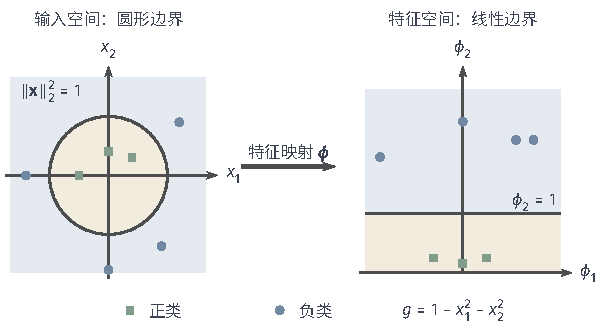
\includegraphics[width=103.166mm]{figures/04-classic-models/00-shared/tikz/classification-kernel-map/figure.pdf}
  \caption{非线性边界在特征映射前后的对应，两个面板的坐标均无量纲。正类方点为$(-0.5,0)$、$(0,0.4)$、$(0.4,0.3)$，负类圆点为$(-1.4,0)$、$(0,-1.6)$、$(1.2,0.9)$、$(0.9,-1.2)$。右图逐点使用$\phi_1=x_1$、$\phi_2=x_1^2+x_2^2$；水平线$\phi_2=1$对应左图半径为1的圆。数据与边界均为教学构造。}
  \label{fig:classification-kernel-map}
\end{figure}

圆形例子只需计算一个新特征，成本可以忽略。但若为了描述更复杂的弯曲关系而加入大量平方项、两两交互项甚至更高次项，显式列出所有新坐标就可能非常昂贵：仅二次映射，$d$ 个原变量就要产生约 $d^2/2$ 个新坐标，次数再升高数量还会快速增长；计算、存储和后续求解都要承担这份开销。于是出现一个关键问题：能不能在不真正写出、也不保存这些新坐标的情况下，照样完成计算？

\emph{从“只需内积”到核展开。}要回答这个问题，先检查线性算法到底怎样使用特征。给定$n$个训练输入$\bm x_1,\ldots,\bm x_n$，设$\bm\phi$将输入映射到带内积的特征空间$\mathcal H$，在那里使用线性得分$\langle\bm w,\bm\phi(\bm x)\rangle+b$。

在一类常见的训练问题里，训练损失只依赖各训练点的得分，而惩罚是参数范数的非减函数。把$\mathcal H$中的任意参数向量分解为“训练特征张成空间内的部分”与“正交于该空间的部分”：正交部分与每个训练特征的内积都是零，把它加到 $\bm w$ 上不会改变任何训练点的得分，却只会增大参数范数，从而增大惩罚。删去这一正交部分，训练得分不变、惩罚不增，因此若最优解存在，总能在这 $n$ 个训练特征张成的空间里找到它（张成空间＝这些特征向量线性组合能够到达的全部方向），即存在一组系数 $a_i$ 使
\begin{equation}
  \bm w=\sum_{i=1}^n a_i\bm\phi(\bm x_i).
  \label{eq:classic-overview-weight-expansion}
\end{equation}
这一展开只说明“有解时解可取在训练特征张成内”，并不单独证明解存在或唯一；存在性与唯一性仍由具体学习目标决定。

把这一展开代回线性得分，内积的线性性质允许把求和提到内积外面：
\begin{equation}
  \begin{aligned}
    K(\bm x,\bm z)
      &=\langle\bm\phi(\bm x),\bm\phi(\bm z)\rangle_{\mathcal H},\\
    f(\bm x)&=\sum_{i=1}^n a_iK(\bm x_i,\bm x)+b.
  \end{aligned}
  \label{eq:classic-overview-kernel}
\end{equation}
这里三者职责不同：核 $K$ 只给出两个输入映射后的特征内积，样本系数 $a_i$ 由具体学习目标确定，截距 $b$ 处理特征均值未被零化的整体偏移。预测时只需逐个计算新输入与训练输入的核值，既不必写出映射后的坐标，也不必保存高维的 $\bm w$。这种用核值完成特征内积计算的办法称为\term{核技巧}（kernel trick）；当$K$对原输入非线性时，特征空间中的线性得分也能描述原空间中的非线性关系，而显式特征展开这一步被完全绕过。

注意，式~\eqref{eq:classic-overview-kernel}只保证“预测”能改写为核值计算；要连训练也一起省去显式特征，训练问题本身也必须只通过核值使用特征。例如训练损失只使用各训练点的得分，并以正系数惩罚参数范数平方时，前面关于正交部分的论证正好适用：正交部分不改变训练得分却增加惩罚，最优解自然落在训练特征张成的空间内，于是整个训练都可用上述有限展开完成。具体到支持向量机，这一对偶形式将在分类章推导。核决定的是特征表示，分类、回归等任务仍由各自的损失和约束确定学习目标。

\subsubsection{合法核、常用核与超参数}
\label{sec:classic-overview-kernel-validity}
\label{sec:classic-overview-common-kernels}

\emph{什么样的函数才能充当核。}从“衡量相似性”的直觉随手设计一个 $K$ 并不困难，但不是每个看起来合理的相似性公式都能作为内积的替代。先注意这里说的“核”是特征内积的代称，与回归章局部加权里“按距离给记录加权重”的核只是同名：那个距离权重核只决定邻域内的加权平均，并不对应某个特征空间。原因在于，$K$ 必须真的等于某个特征空间中的内积，而内积有不能违反的代数性质。

内积首先是对称的：$\langle\bm u,\bm v\rangle=\langle\bm v,\bm u\rangle$。更重要的是，任意特征向量线性组合的长度平方都不可能为负。因此，对任意有限个输入$\bm x_1,\ldots,\bm x_m$和任意实系数$c_1,\ldots,c_m$，必须有
\[
  \begin{aligned}
    \sum_{i,j=1}^m c_ic_jK(\bm x_i,\bm x_j)
      &=\left\lVert\sum_{i=1}^m c_i\bm\phi(\bm x_i)\right\rVert^2\\
      &\geq0.
  \end{aligned}
\]
将这些输入的核值排成矩阵，称为这组输入的\term{Gram矩阵}（Gram matrix），也就是两两特征内积组成的矩阵；上述条件等价于矩阵对称且半正定，即用任意实向量 $\bm c$ 左乘右乘都不会得到负数。

反过来，若一个对称函数在整个预期输入域上对每一组有限输入都满足“Gram矩阵半正定”，就可以从形式特征的有限线性组合出发构造半内积（允许某个非零向量范数为零的退化内积），再把零范数的等价类消去、对空间完备化（补上所有极限点，使空间闭合），得到一个以该核为内积的特征空间。这里只交代存在性依据；连续性等Mercer定理的附加条件是针对特定定义域与连续核的进一步要求，不能误列为所有合法核的必要条件。本书将这样的函数称为正定核（positive definite kernel），允许有限核矩阵奇异（即存在非零 $\bm c$ 使二次型为零），不额外要求矩阵可逆。

合法性检查的是“所有实系数形成的二次型是否非负”，要避免几种常见误解。它不是检查每个核值本身是否非负——合法核在不相似的两点上完全可以取负值（例如未加常数的线性核）。它也不是凭“看起来像相似性”就能成立。只检查某一份训练集上的矩阵，只能确认这一组输入合法；新输入还必须落在核已确认合法的定义域内。此外，合法核只提供“它确实对应某个特征内积”的依据，并不保证这个特征表示适合当前任务，也不保证对应的学习目标容易求解——合法性与有效性是两件事。

对$\bm x,\bm z\in\mathbb R^d$，选择不同的核，等于暗中选择了不同的特征空间和特征关系。表\ref{tab:classic-overview-common-kernels}列出常见形式及条件；核尺度记为$\beta$，多项式次数记为$p$，与输入维数$d$区分。

\begin{table}[htbp]
  \centering
  \small
  \begin{tabularx}{\linewidth}{@{}>{\RaggedRight\arraybackslash}p{18mm}>{\RaggedRight\arraybackslash}X>{\RaggedRight\arraybackslash}p{27mm}@{}}
    \toprule
    名称 & $K(\bm{x},\bm{z})$ & 参数与正定性\\
    \midrule
    线性核 & $\bm{x}^{\top}\bm{z}$ & 半正定\\
    多项式核 & $(\beta\bm{x}^{\top}\bm{z}+r)^p$ & $\beta,r\ge0$，正整数$p$\\
    高斯RBF核 & $\exp(-\beta\lVert\bm{x}-\bm{z}\rVert_2^2)$ & $\beta>0$，半正定\\
    Laplacian核 & $\exp(-\beta\lVert\bm{x}-\bm{z}\rVert_1)$ & $\beta>0$，半正定\\
    Sigmoid形式 & $\tanh(\beta\bm{x}^{\top}\bm{z}+r)$ & 一般不保证半正定\\
    \bottomrule
  \end{tabularx}
  \caption{常用核函数与合法性条件。这里的“半正定”要求任意有限输入的Gram矩阵半正定；Sigmoid一行列出的是常见相似性形式，使用前仍需针对定义域与参数核验。}
  \label{tab:classic-overview-common-kernels}
\end{table}

\term{线性核}（linear kernel）就是原始特征的内积，不增加任何新特征，对应普通的线性模型，常作为比较基准。\term{多项式核}（polynomial kernel）隐式加入了有限阶的特征交互：把 $(\beta\bm x^\top\bm z+r)^p$ 展开后，各项对应原变量的各次乘积，因此 $p=2$ 时能表达平方项和两两乘积，$p$ 更大时表达更高次的组合。在$\beta>0$时，$r=0$只保留$p$次项，$r>0$则包含从常数项到$p$次项的各阶特征；参数取零时，相应特征块可以消失。核计算省去的是这些坐标的显式展开，完整训练成本仍取决于样本数和学习目标。

\term{高斯径向基核}（Gaussian radial basis function kernel，Gaussian RBF kernel）不看方向上的投影，而按两点的欧氏距离衡量局部接近程度：两点重合时核值为 $1$，距离越远核值平滑衰减到 $0$。常将$\beta$写成$1/(2\sigma^2)$，其中$\sigma>0$是距离尺度：$\sigma$ 越大（$\beta$ 越小），核值衰减越慢，一个点能影响的范围越宽；$\sigma$ 越小（$\beta$ 越大），作用范围越局部。它对应的特征空间是无限维的，因而能表达相当灵活的非线性关系，但作用范围是否合适仍需结合数据判断，不能仅凭“能拟合弯曲边界”就断定新样本误差更小。

\term{Laplacian核}（Laplacian kernel）形式相近，只是把欧氏距离换成$L^1$距离，即各坐标绝对差之和；$L^1$距离沿坐标轴方向变化，改变了衡量“接近”的几何，对某些坐标轴对齐的结构更敏感。

常称为\term{Sigmoid核}（sigmoid kernel）的形式把内积送入双曲正切函数，在神经网络兴起后常被使用，但它一般不保证正定核所需的半正定性；只取正参数也不足以替代对定义域和参数取值的合法性核验，使用前必须单独检查或改用其他核。核尺度、多项式次数、正则化强度等在一次拟合前固定的配置，可以用验证数据在训练内选择；配置确定后，还要用未参与选择的新数据评价预测误差，不能把选择配置时用过的数据再当作最终评价依据。

\subsubsection{核矩阵与训练中心}
\label{sec:classic-overview-kernel-matrix}

把预测公式用于全部训练点，可以看出核方法的规模压力落在哪里。训练时，将$n$个输入两两之间的核值排成训练Gram矩阵$\bm K\in\mathbb R^{n\times n}$，其中$\bm K_{i,j}=K(\bm x_i,\bm x_j)$。令$\bm a=(a_1,\ldots,a_n)^{\top}$、$\bm1\in\mathbb R^n$为全一向量，式\eqref{eq:classic-overview-kernel}在训练点上的预测便是$\bm K\bm a+b\bm1$。完整存储这个矩阵需要$O(n^2)$空间，构造它需要$O(n^2)$次核计算；也就是说，核技巧把“显式展开可能极高维的特征”的压力，转换成了“成对计算并存储样本关系”的压力，后续求解线性或二次问题的成本还要另外计算。当样本量很大时，这一 $n^2$ 规模往往比特征维数更先成为瓶颈，省去显式坐标并不等于没有计算代价。

有些学习目标要求比较样本围绕共同中心的变化，而不是它们相对原点的绝对位置。例如核PCA要在特征空间中找“数据散布最大的方向”，这一分析应当围绕特征均值进行；原点位置改变不应影响结论。这时需要在特征空间中减去训练均值。训练特征均值与各点的偏离量为
\[
  \bar{\bm\phi}=\frac1n\sum_{i=1}^n\bm\phi(\bm x_i),
  \qquad
  \widetilde{\bm\phi}_i=\bm\phi(\bm x_i)-\bar{\bm\phi}.
\]
中心化后的内积仍可只用核值计算。令$\bm I_n$为单位矩阵，中心化矩阵和中心化核矩阵为
\begin{equation}
  \bm H=\bm I_n-\frac1n\bm1\bm1^{\top},
  \qquad \bm K_{\mathrm c}=\bm H\bm K\bm H.
  \label{eq:classic-overview-kernel-centering}
\end{equation}
矩阵 $\bm H$ 的作用就是“减去平均值”：左乘或右乘 $\bm H$ 相当于减去行均值或列均值。有限维特征按行排成矩阵$\bm\Phi$时，减去每列训练均值得到$\bm H\bm\Phi$，其Gram矩阵就是$\bm H\bm\Phi\bm\Phi^{\top}\bm H=\bm H\bm K\bm H$。即使特征空间是无限维的，无法写出矩阵 $\bm\Phi$，直接展开中心化特征的内积也得到同一个公式 $\bm H\bm K\bm H$，这正是核技巧的价值所在。还要注意，非线性映射与减均值一般不能交换次序，因此只在原输入空间做中心化，并不能代替在特征空间中的这一步。

新输入$\bm x$在预测时也必须减去同一个训练特征均值，保持训练和预测使用共同参照；不能为每个新查询重新定义中心，否则训练得到的坐标与预测坐标不在同一参照系中。它与第$i$个训练输入的中心化核值为
\[
  \begin{aligned}
    K_{\mathrm c}(\bm x_i,\bm x)
      ={}&K(\bm x_i,\bm x)
       -\frac1n\sum_{j=1}^n K(\bm x_i,\bm x_j)\\
       &-\frac1n\sum_{j=1}^n K(\bm x_j,\bm x)
       +\frac1{n^2}\sum_{j,l=1}^n K(\bm x_j,\bm x_l).
  \end{aligned}
\]
四项可以逐项对照 $\langle\bm\phi(\bm x_i)-\bar{\bm\phi},\bm\phi(\bm x)-\bar{\bm\phi}\rangle$ 的展开来理解：第一项是原内积，第二、三项分别扣除两个端点与训练均值的内积，最后一项把均值自身的内积加回来，因为它在前两步里被减了两次。所有求和都固定使用训练输入，新点不参与均值的计算。是否中心化由学习目标决定：核PCA这类分析围绕特征均值变化的方法需要中心化，而直接做分类、回归的核方法未必需要；采用核并不意味着所有方法都执行同一套中心化流程。


\subsection{邻域方法：参考查询附近的记录}
\label{sec:classic-overview-neighborhood}

与“用一个全局加权和概括所有样本”相反，邻域方法只看查询点附近的少量记录。要估计一套从未见过的房屋价格，找出与它面积、房龄最接近的若干套已成交房屋，用它们的成交价作平均；要判断一封新邮件是否垃圾邮件，找出词频分布最接近的若干封已标注邮件，按多数类别投票。这里不假设一条统一的关系曲线贯穿全部样本，只相信邻近的记录提供局部答案。

邻域方法需要决定三件事：保留哪些训练记录、用什么距离衡量接近、怎样组织记录以便快速找到邻居。距离可以是各属性差的平方和开方，也可以是按重要性加权后的距离；“近”的定义不同，选出的邻居就不同。聚类、图表示与半监督学习都可以复用这种邻近关系，但它们还需要各自的输出规则：聚类把邻近关系组织成群组，半监督把邻近关系传播到未标注点，不能把“找邻居”本身当成最终任务。

\subsection{树与规则：按输入条件选择局部预测}
\label{sec:classic-overview-trees-rules}

树方法把输入空间按一系列条件切成小块：先问面积是否超过某个值，再在每一块里问房龄或地段，逐层细分，直到每个叶块里的样本足够同质。预测时沿条件一路走到某个叶块，输出该块内的代表值（回归取均值，分类取多数类）。规则方法是同一思想的平铺形式：用“若面积大且地段好，则价格高”这样的条件组合直接给出判断。

与全局加权和相比，树不需要把整个空间套进一条直线或一个曲面，弯曲关系由一系列分段直线拼接出来；与邻域方法相比，树的划分边界由数据按准则选出，而不是预先固定一个邻域半径。它的代价是叶块之间可能出现阶梯状跳变，且每个叶块内的样本量决定了代表值是否稳定。

\subsection{概率模型：区分响应波动与参数不确定性}
\label{sec:classic-overview-probability}

前面几类方法直接给出一个预测值；概率模型还进一步描述这个值的波动。对一套给定的房屋，成交价本身在不同交易中会有起伏，概率模型为每个输入写出响应的分布，而不只是一个点估计；例如把条件分布写成$p(y\mid\bm x;\bm\theta)$，$\bm\theta$是分布参数。

参数的不确定性用先验与后验表达：先验$\pi(\bm\theta)$描述估计前对参数的认识，似然$p(\text{数据}\mid\bm\theta)$描述数据怎样由参数产生，贝叶斯定理把两者结合成后验$p(\bm\theta\mid\text{数据})$。这里要区分两种不确定：响应波动是给定参数后$y$自身的随机，参数不确定性是$\bm\theta$尚未被数据唯一确定；判别模型直接建模$p(y\mid\bm x)$，生成模型先建模$p(\bm x,y)$再推出条件分布，两者对不确定性的处理位置不同。概率模型还可以引入未被观测的潜成分（混合分量、隐变量），连续隐变量与降维的坐标表示相互衔接。

\subsection{集成方法：组合多个预测}
\label{sec:classic-overview-ensemble}

单个模型的预测可能因训练波动或遗漏结构而不稳定，集成方法训练多个成员，再把它们的输出组合成一个结果。按成员怎样产生、怎样组合，本书区分三条路线：让成员在略有不同的数据上独立训练再平均（Bagging、随机森林）；让成员逐个产生，每一个专门修正前面组合的错误（Boosting）；让数据自己学会怎样组合已有成员的预测（Stacking）。三条路线的共同问题是成员之间的相关性、组合规则带来的偏差与部署成本，完整机制在第\ref{chap:ensemble-learning}章展开。

\section{研究历史}
\label{sec:classic-history}

本节按五个阶段梳理经典模型的发展脉络，目的是定位思想、避免错置归属：同一时期的工作面对的问题不同，不同阶段的方法也并非按一条直线替代。历史不重讲各模型的正式推导，那些推导属于各自章节。

\subsection{统计估计与多元分析的形成（19世纪初—1940年代）}
\label{sec:classic-history-estimation}

最小二乘法在19世纪初同时由勒让德与高斯发展出来：把多次观测的误差平方相加，取使总和最小的参数作为估计；观测由此通过同一个共同准则汇总，而不是各自为政\scite{legendre1805,gauss1809}。图\ref{fig:classic-history-observations}给出这一思想的场景：一组观测围绕待估数值散布，最小二乘选择让各误差平方和最小的位置。这里只说明平方准则在历史上怎样被用来取舍观测；它为什么恰好导向均值、在什么概率假设下等价于最大似然估计，留到第\ref{chap:regression}章推导。

\begin{figure}[htbp]
  \centering
  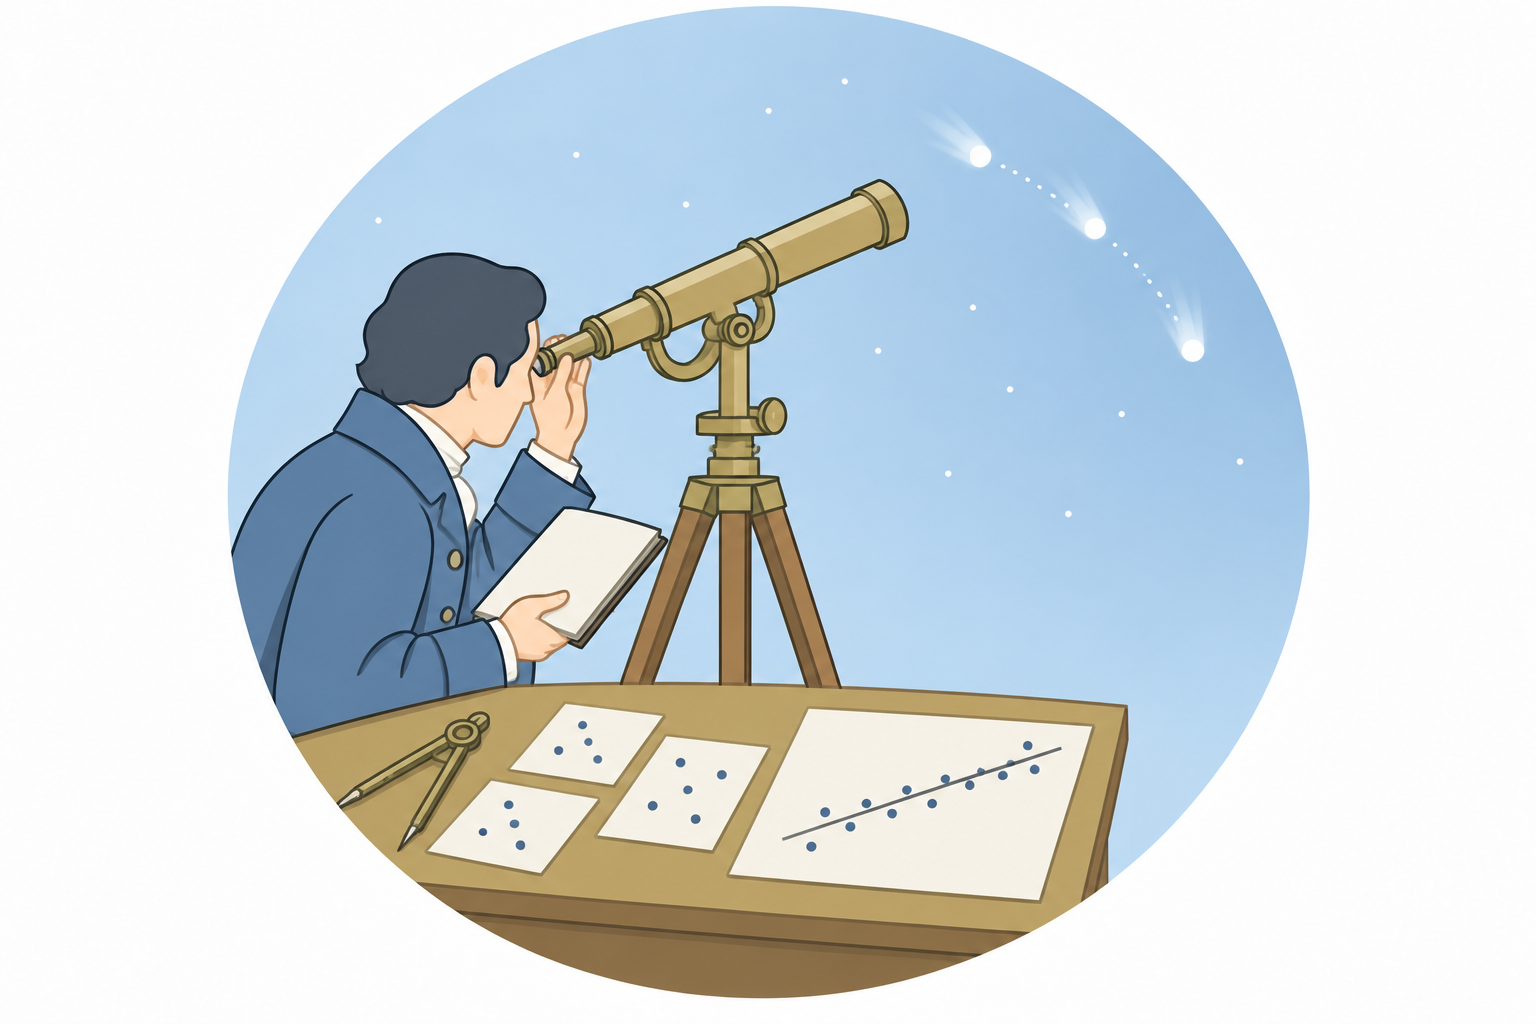
\includegraphics[width=94mm]{figures/04-classic-models/00-shared/generated/least-squares-observations/figure.png}
  \caption{围绕待估数值的多次观测（教学构造）：竖线为观测位置，黑色圆点为最小二乘估计位置；残差为观测到估计位置的水平差。}
  \label{fig:classic-history-observations}
\end{figure}

19世纪末高尔顿在亲子身高数据中观察到“向均值回归”的现象，催生了回归这一概念\scite{galton1886}。进入20世纪，皮尔逊1901年从几何拟合角度提出主成分分析，霍特林1933年把它发展为保留输入自身方差的正交坐标\scite{pearson1901pca,hotelling1933pca}；费舍尔1936年的判别分析与拉奥1948年的推广，则面向“怎样把不同类别分开”的目标\scite{fisher1936,rao1948}。图\ref{fig:classic-history-iris}展示的鸢尾花测量数据，正是费舍尔工作使用的经典多元样本。

\begin{figure}[htbp]
  \centering
  
\includegraphics[width=94mm]{figures/04-classic-models/00-shared/generated/iris-measurements/figure.png}
  \caption{三种鸢尾花的花瓣长度与花瓣宽度测量（教学示意，坐标轴无量纲）：不同类别在平面上有部分重叠，可分方向与方差较大的方向并不完全一致。}
  \label{fig:classic-history-iris}
\end{figure}

这一阶段形成了两条并行的研究目标：一条从观测误差出发估计共同参数（回归），另一条处理多变量的结构——要么保留输入自身的变化（主成分），要么区分给定类别（判别）。两者使用相似的几何工具，但优化目标不同，这一区分贯穿后续各章。

\subsection{模式识别与样本学习（1950—1960年代）}
\label{sec:classic-history-pattern}

1958年罗森布拉特提出感知机，用样本反馈直接调整线性分类的系数，标志着从“预设统计分布”转向“从样本中学习判别规则”\scite{rosenblatt1958}；几乎同时，基于邻近样本投票的早期近邻分类思路出现，而Cover与Hart在1967年给出的是近邻规则的错误率分析，并非近邻思想的首次提出，引用时不应把二者混为一谈\scite{coverhart1967}。1967年MacQueen提出以中心为代表的K-means聚类，它与监督判别使用的信息不同：没有类别标签，只按到中心的距离分组\scite{clust-macqueen1967}。

同一时期，Aizerman等人1964年的势函数方法已经把非线性特征与按样本展开的系数结合起来，是后来核表示的早期线索；但它与1990年代以间隔为准则的支持向量机属于不同问题，不能把核思想的形成全部归到1990年代\scite{aizerman1964potential}。这一阶段的共同特征是：模型直接面对样本，学习规则由样本驱动，而不是先假定完整的分布形式。

\subsection{灵活建模与计算统计（1970—1980年代）}
\label{sec:classic-history-flexible}

1972年Nelder与Wedderburn的广义线性模型把响应分布、链接函数与线性预测项统一起来，使回归不必局限于正态响应与恒等链接\scite{nelder1972glm}；Cleveland1979年的稳健局部加权回归用邻近样本的局部拟合替代一条全局直线\scite{cleveland1979lowess}；Hastie与Tibshirani1986年的广义加性模型则把单个变量的平滑效应逐项相加，放松了全局线性的约束\scite{hastie1986gam}。三者分别从响应分布、局部拟合和变量平滑三个方向扩展了全局线性模型，相应的公式在回归章展开。

1977年Dempster、Laird与Rubin系统给出EM算法的命名与迭代估计框架，为混合模型与含潜变量的估计提供了统一思路；但EM不是这一时期唯一的迭代估计算法，只应把它放在“系统化”的位置上\scite{clust-dempster1977}。1984年Breiman等人的CART专著系统整理了树的生长与剪枝，使按输入条件分区的模型有了可操作的估计流程\scite{breiman1984cart}。与分布模型、平滑模型并行，计算搜索让灵活结构成为可能，是这一阶段的共同背景。

\subsection{统计学习、非线性表示与集成（1990年代）}
\label{sec:classic-history-statistical}

1991年Friedman的MARS用自适应分段基函数表达非线性交互\scite{friedman1991mars}；1995年Cortes与Vapnik的支持向量网络以最大间隔为准则，把早期核表示与分类目标结合起来\scite{cortes1995}。这一阶段的关键词是自适应表示、间隔准则与容错训练；但核的非线性特征早在势函数时期已经出现，不能把相关思想都记在1990年代。聚类一侧，1996年Ester等人的DBSCAN提出按密度分组，与以中心划分、以混合模型拟合的路线在历史上形成对照\scite{ester1996}。

集成的三条路线也在这一阶段成型：Wolpert1992年提出Stacking，让数据学习成员怎样组合\scite{wolpert1992stacked}；Breiman1996年的Bagging通过随机扰动样本再聚合\scite{breiman1996bagging}；AdaBoost在1990年代初被提出，Freund与Schapire1997年的论文给出系统表述\scite{freund1997boosting}。三者分别对应学习组合、随机扰动聚合与顺序修正，第六章分别展开。

\subsection{非线性表示与规模化学习（2000年代以来）}
\label{sec:classic-history-scaling}

2000年的Isomap与局部线性嵌入（LLE）把全局线性的坐标表示推广到非线性流形：Isomap利用测地距离，LLE利用局部邻域关系重构坐标，具体准则在降维章推导\scite{dimTenenbaum2000,dimRoweis2000}。集成一侧，2001年Breiman的随机森林在自助采样之外加入节点级特征随机化，同年Friedman的梯度提升以负梯度方向逐轮拟合\scite{breiman2001randomforests,friedman2001gradientboost}；随后2016年的XGBoost、2017年的LightGBM把样本规模与训练成本作为明确的学习问题处理\scite{chen2016xgboost,ke2017lightgbm}。各自贡献分别对应成员随机化、顺序修正与计算组织，不合并为一个笼统的“提升方法”。

图\ref{fig:classic-models-history}按阶段汇总本节选取的代表工作。阅读这张图时按阶段定位即可，不要把不同年代的工作排成一条线性优劣序列；图中区分了思想提出、论文发表、系统化表述与理论分析各自可能相隔的时间。

\begin{figure*}[htbp]
  \centering
  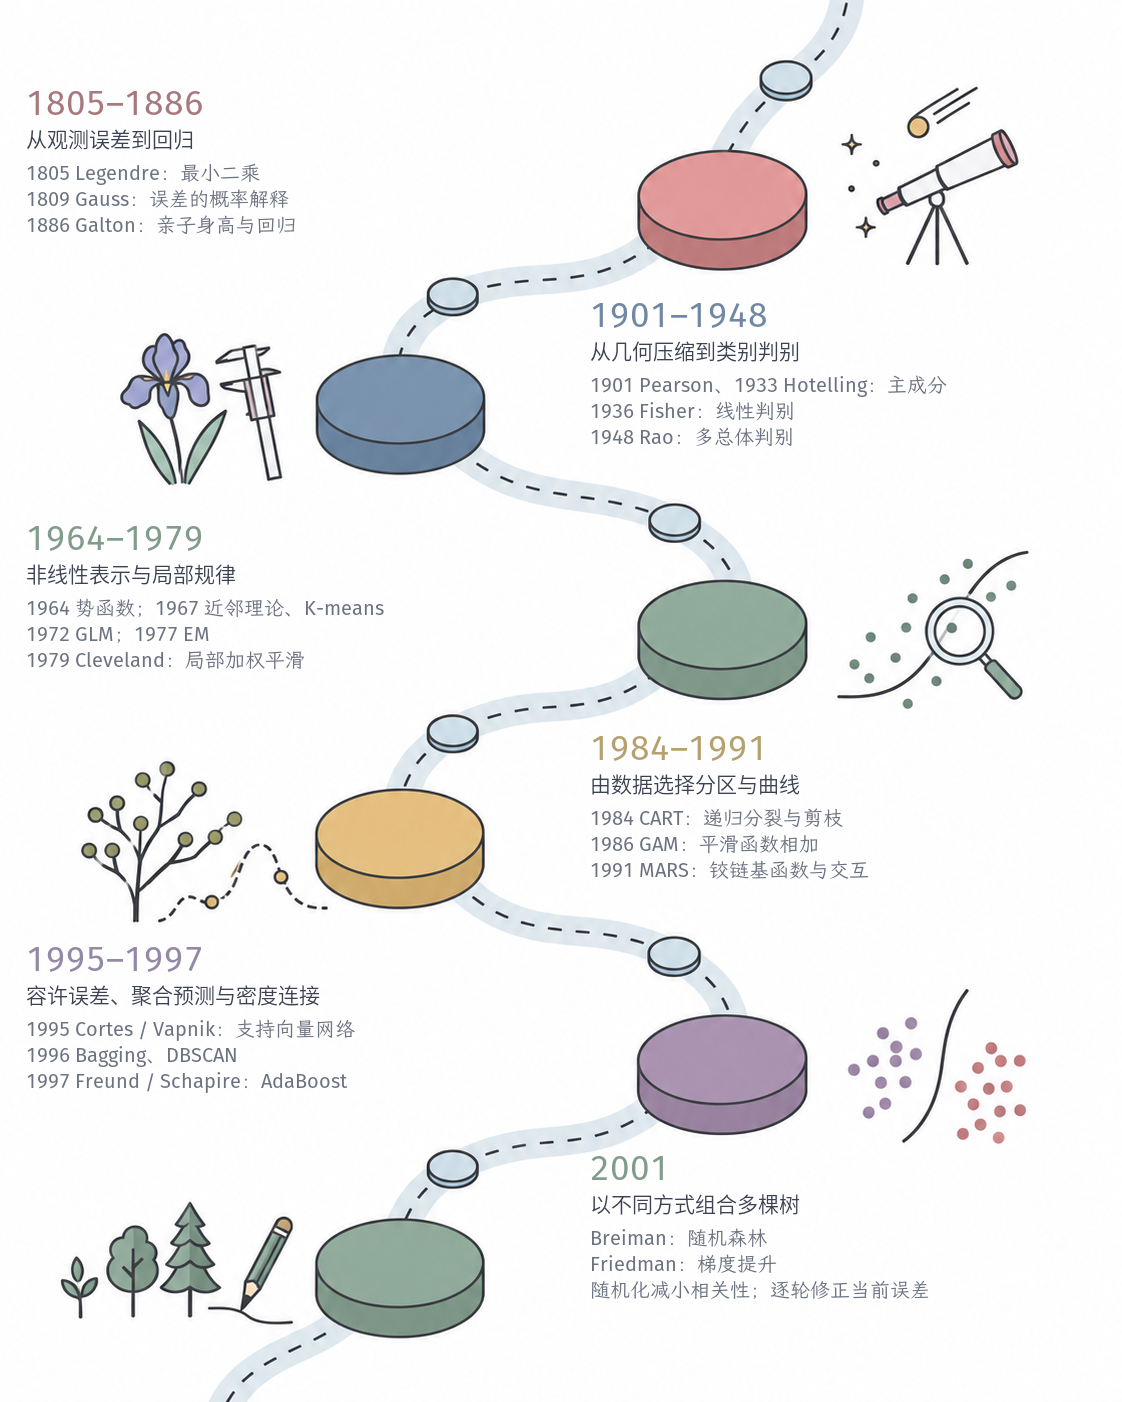
\includegraphics[width=157.406mm,height=.88\textheight,keepaspectratio]{figures/04-classic-models/00-shared/generated/classic-models-history/figure.png}
  \caption{经典模型代表工作的阶段分布（示意）。同一项工作的思想提出、发表、系统化与理论分析可能落在不同年份；图中只选取本节涉及的代表，不代表完整编年，也不按年代排序优劣。}
  \label{fig:classic-models-history}
\end{figure*}

\FloatBarrier
\section{本章小结}
\label{sec:classic-overview-summary}

任务决定模型的输出：回归给数值、分类给类别、聚类给群组、降维给坐标；输出不同，损失与评价对象随之不同，不能把估计均值、预测类别、分组与压缩坐标混为一个“拟合好坏”。本章按计算关系比较了特征加权、核方法、邻域、树与规则、概率模型与集成六类常见方法，每一类只交代核心计算与边界，表示如何学习、目标如何优化留待各章。

核的一般定义、合法核的半正定依据、有限展开的成立条件、核矩阵规模与训练中心化已在本章建立；核只决定特征表示，具体学习目标由任务章节给出。历史部分按五个阶段定位了估计与多元分析、模式识别与样本学习、灵活建模与计算统计、统计学习与集成、非线性表示与规模化学习中的代表工作，避免把不同问题、不同年代的思想错置归属。

后续章节按输出展开：回归章从数值响应落实“表示关系—学习参数—评价效果”的完整流程，此后依次进入分类、聚类、降维与集成学习。

\paragraph{扩展阅读}
一般统计学习教材可作为概念对照\scite{hastie2009,bishop2006}；历史归属以原始论文发表信息为准，本章不新增文献条目。

\chapter{回归}
\label{chap:regression}

预测房屋价格时，可以估计平均成交价，也可以给出预算所需的上分位数或价格分布。\term{回归}（regression）根据输入估计数值响应的这些条件特征。设训练集为$D_n=\{(\bm{x}_i,y_i)\}_{i=1}^{n}$，其中$\bm{x}_i\in\mathbb{R}^{d}$为输入，$y_i\in\mathbb{R}$为响应，预测函数记为$f$；响应也可以是次数等离散数值。

需要检查变量作用或建立简洁基线时，可以从线性模型开始；关系随输入区域变化时，则考察局部回归、树或平滑函数。若决策还需要尾部阈值或分布信息，预测对象也要相应改变。

预测对象确定以后，还要选择输入与响应之间的关系。全局加权适合描述共同趋势，邻域方法在查询点附近估计响应，树与规则为不同条件分配局部预测，概率模型保留分布信息。各节沿着这些关系展开训练目标与求解过程，再考察新输入上的预测误差。第\ref{chap:classic-models-overview}章建立的建模思路，在这里由数值响应及其损失具体化。

阅读本章时可以抓住两条线索。第一条是“到底想预测响应分布的哪个位置”：默认预测条件均值，需要控制超支风险时转向条件分位数，容忍小偏差时只惩罚落在容忍带外的误差，需要完整不确定性时再估计响应分布或预测区间。预测对象不同，给误差计分的损失函数就不同。第二条是“用什么形状的函数去表示关系”：先从最容易估计也最容易解释的线性加权开始；当直线不足以描述曲率或交互时，依次尝试展开特征、参考附近样本、按条件分区，最后用概率模型描述整条函数的不确定性。本章各节正是按这两条线索的交点组织的——同一个函数表示可以搭配不同损失，同一种损失思想也能用于不同表示，因此不要把“某个模型”和“某个预测目标”混为一谈。

\section{基于线性关系的回归}
\label{sec:regression-linear}

预测房价的一个起点是给输入特征赋予权重，用加权和表示整体趋势。要由数据选出权重，就需要规定什么误差值得减小，以及多大的系数变化可以接受。最小二乘用平方残差评价拟合，正则化限制系数，分位数回归和SVR则改变误差的计分方式。原特征的线性关系不足时，还可以增加基函数或采用核；响应的取值范围与分布特征，则由GLM和GAM进一步处理。

这一小节包含的模型较多，它们其实只在回答三个依次出现的问题，按这个顺序阅读就不会迷失。第一，给定一组固定特征，怎样选出一组权重？普通最小二乘给出最基本的答案，并讨论它的两种求解方式和直线表示能力不足时的特征展开。第二，特征彼此高度相关时，最小二乘的权重会剧烈摆动怎么办？正则化通过给系数增加代价来稳定估计，成分回归则换个角度先压缩特征方向。第三，如果预测目标根本不是条件均值（要分位数、要容忍带、响应取值受限或作用本身弯曲），就要相应更换损失或响应模型，这对应分位数回归、SVR、GLM和GAM。

\subsection{普通最小二乘（OLS）}
\label{sec:regression-ols}

同一输入可能对应不同的观测响应，因而很难找到一条穿过所有样本的直线。考虑四个教学样本：$x=0$处的响应为$2,4$，$x=1$处的响应为$4,6$。两处各有两个不同数值，精确插值已经不可能；我们需要一个规则，在这些不一致的观测之间选择预测。若用平方残差计分，两个位置分别取均值$3,5$最合适，对应直线$f(x)=3+2x$。

\term{普通最小二乘}（ordinary least squares, OLS）把这种选择推广为寻找残差平方和最小的系数。平方损失让正、负误差受到相同惩罚，也让大误差付出更高代价。它可以作为无需指定响应分布的拟合准则；在独立、零均值且同方差的高斯误差下，又可解释为最大似然估计。先建立固定特征下的拟合与求解，再考察特征形状、观测精度和异常响应怎样改变这个问题\scite{bishop2006}。

\subsubsection{模型结构}
\label{sec:regression-ols-structure}

令$\bm{\phi}(\bm{x})\in\mathbb{R}^{p}$表示固定特征向量，模型写成$f_{\bm{w}}(\bm{x})=\bm{\phi}(\bm{x})^{\top}\bm{w}$，其中$\bm{w}\in\mathbb{R}^{p}$。最简单的选择是$\bm{\phi}(\bm{x})=(1,\bm{x}^{\top})^{\top}$，此时$p=d+1$，第一个系数为截距。这里的“线性”指预测对待估计系数线性；特征变换$\bm{\phi}$可以非线性，其具体形式将在本小节后面展开。

把样本堆叠为设计矩阵$\bm{X}\in\mathbb{R}^{n\times p}$，第$i$行为$\bm{\phi}(\bm{x}_i)^{\top}$，并记$\bm{y}=(y_1,\ldots,y_n)^{\top}$，得到目标
\begin{equation}
  \widehat{\bm{w}}\in\argmin_{\bm{w}}J(\bm{w}),
  \qquad
  J(\bm{w})=\frac{1}{2n}\lVert\bm{y}-\bm{X}\bm{w}\rVert_2^2.
  \label{eq:regression-ols-objective}
\end{equation}
因子$1/(2n)$不改变OLS的最优解，但会影响梯度、步长和正则系数的数值约定。本章使用平均平方损失时均沿用这一形式。

图\ref{fig:regression-ols-residuals}把这个目标放回输入与响应平面：每条虚线都是固定$x_i$之后，观测$y_i$与直线预测之间的纵向差。OLS选择的是让这些差的平方和最小的直线，因此拟合线通常不穿过每个样本；图中的距离沿响应轴测量，区别于点到直线的垂直几何距离。

\begin{figure}[htbp]
  \centering
  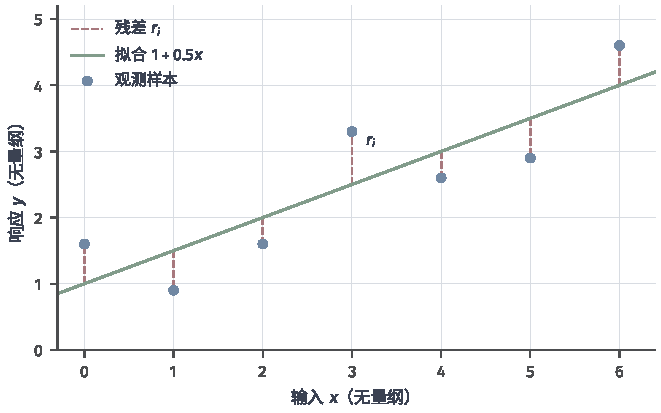
\includegraphics[width=105.412mm]{figures/04-classic-models/00-shared/matplotlib/regression-ols-residuals/figure.pdf}
  \caption{一维OLS与响应残差。七个构造样本的最小二乘直线为$\widehat f(x)=1+0.5x$；蓝色实心点表示观测，绿色实线表示预测，红色竖虚线表示$r_i=y_i-\widehat f(x_i)$。横、纵轴均为无量纲教学变量。}
  \label{fig:regression-ols-residuals}
\end{figure}

手中的残差平方和只评价已经观测到的记录。需要提醒的是，把训练误差压到零并不难，也往往不是目的：只要模型足够灵活（比如让一条折线穿过每个训练点），训练误差就能为零，但这条折线在任意两个训练点之间的取值毫无依据，换一批数据得到的折线也完全不同。若要判断预测函数面对未来记录时怎样，就要按未来输入与响应的共同分布，计算平方损失的平均值$\mathbb E[(Y-f(\bm X))^2/2]$；这种未来平均损失称为期望风险（expected risk）。先固定一个输入$\bm x$，把该输入处的条件均值记为$m(\bm x)=\mathbb E[Y\mid\bm X=\bm x]$。对任意实数预测$a$，条件平方误差可拆成
\[
 \begin{aligned}
 &\mathbb E[(Y-a)^2\mid\bm X=\bm x]\\
 &\quad=\operatorname{Var}(Y\mid\bm X=\bm x)
             +[m(\bm x)-a]^2.
 \end{aligned}
\]
第一项是固定输入后响应自身的波动，不随$a$改变；第二项在$a=m(\bm x)$时最小。再按未来输入出现的频率平均，就解释了平方损失为何以条件均值为预测目标，而不是以每条带噪响应为必须穿过的点。

响应二阶矩有限时，条件均值在平方可积预测函数中达到最小风险，且只在输入分布的几乎处处意义下唯一，可参考\BookChapterRef{chap:random-variables}{卷二《数学准备：概率、因果与决策》的“随机变量”章}。
限制为$f_{\bm w}$以后，若条件均值不属于所选模型类，OLS估计的只是该类中的平方逼近；
高斯性、同方差性与误差对称性都不是平方损失以条件均值为目标的必要条件。
这里的平方可积要求函数值的平方具有有限期望。“几乎处处”允许函数在输入概率为零的集合上不同，因为这种差异不会改变上述平均损失。总体中的最佳候选与有限数据算出的系数仍有区别：OLS用训练记录的平均损失估计这个总体目标，某一次样本得到的最优函数未必就是总体中最近的候选。

\subsubsection{参数学习}
\label{sec:regression-ols-learning}

OLS的参数学习有两条路线。一条路线直接求出最优系数的方程，再用矩阵分解解方程；另一条路线从初始系数出发，反复减小训练损失。

先看第一条：式\eqref{eq:regression-ols-objective}是一个无约束、可微的凸二次目标。“凸”意味着它的等高线像碗的内壁，从任意点沿碗壁向下走都不会掉进某个只在局部最低的小坑；因此只要找到坡度恰好为零的位置，就能确认这是全局最低点，而不必担心别处还有更低的解。在最小点处，每个系数方向上的一阶变化都应为零。对残差平方求导得到
\[
  \nabla J(\bm w)=\frac1n\bm X^\top(\bm X\bm w-\bm y),
  \qquad \nabla^2J(\bm w)=\frac1n\bm X^\top\bm X.
\]
第二个矩阵半正定，说明目标凸；因此梯度为零不仅是必要条件，也足以认证全局最优。把第一式置零，就得到\term{正规方程}（normal equations）。它要求残差与每一列特征正交：沿任何已提供的特征方向调整系数，都不能再降低平方误差。
\begin{equation}
  \bm{X}^{\top}\bm{X}\widehat{\bm{w}}=\bm{X}^{\top}\bm{y}.
  \label{eq:regression-normal-equations}
\end{equation}

若$\bm X\bm v=\bm0$，将$\bm v$加到系数上不会改变训练预测。所有这类向量组成设计矩阵的零空间，记为$\operatorname{null}(\bm X)$。还可以在全部最小二乘解中选择长度最小的代表，写为$\bm X^\dagger\bm y$；符号$\dagger$表示Moore--Penrose伪逆（Moore--Penrose pseudoinverse），它在这里把响应向量送到这个最小范数代表。解集因而可以读成“一个代表加上任意训练不可见的方向”。

正规方程的全部参数解为$\bm X^\dagger\bm y+\operatorname{null}(\bm X)$，可参考\BookChapterRef{chap:linear-algebra-and-matrix-analysis}{卷一《数学准备：计算、分析与几何》的“线性空间”章}。
因此训练拟合值总是唯一，参数唯一则要求设计矩阵列满秩；否则可取最小范数解。
零空间中的参数差在训练点上不可见，却可能在新特征向量上产生不同预测。

闭式表达用于分析，计算时通常不显式求逆。列满秩且$n\geq p$时，薄QR分解$\bm{X}=\bm{Q}\bm{R}$把问题化为三角方程$\bm{R}\widehat{\bm{w}}=\bm{Q}^{\top}\bm{y}$，稠密计算代价约为$O(np^2)$。

这里$\bm Q\in\mathbb R^{n\times p}$的列是标准正交的，满足$\bm Q^\top\bm Q=\bm I_p$；$\bm R\in\mathbb R^{p\times p}$为可逆上三角矩阵。“薄”表示只保留张成训练列空间所需的$p$列。把响应分成该空间内外两部分，就有
\[
 \begin{aligned}
 \lVert\bm y-\bm Q\bm R\bm w\rVert_2^2
 &=\lVert\bm Q^\top\bm y-\bm R\bm w\rVert_2^2\\
 &\quad+\lVert(\bm I_n-\bm Q\bm Q^\top)\bm y\rVert_2^2.
 \end{aligned}
\]
第二项不随系数改变，第一项可以令其为零，所以只需回代求解上述三角方程。这条路线没有先把设计矩阵乘成正规方程矩阵。

奇异值分解（singular value decomposition，SVD）则把设计写成$\bm X=\bm U_r\bm D_r\bm V_r^\top$，其中$r$为秩，$\bm U_r$与$\bm V_r$各有$r$列标准正交向量，$\bm D_r$的对角元$s_1,\ldots,s_r$为正奇异值。系数空间中的方向$\bm v_j$经过设计矩阵后满足$\bm X\bm v_j=s_j\bm u_j$：$\bm u_j$位于训练预测空间，$s_j$表示系数沿该方向改变时，训练预测被放大多少。奇异值很小，就意味着较大的系数变化只产生较小的训练变化；零空间方向则完全不可见。
最小范数解因此可以按各方向直接计算：
\[
 \bm X^\dagger\bm y
 =\sum_{j=1}^r\frac{\bm u_j^\top\bm y}{s_j}\bm v_j.
\]
先把响应投到$\bm u_j$方向，再除以该方向的放大倍数$s_j$，就还原对应系数；训练不可见的零空间分量取零。小$s_j$也会放大响应中的噪声，这正是病态方向难以估计的原因。

秩亏或需要检查小奇异值时可以用SVD。直接形成$\bm{X}^{\top}\bm{X}$会把满列秩矩阵的二范数条件数平方，因此近似共线时尤其应避免求逆实现。
满列秩时，这个条件数是最大与最小奇异值之比$s_{\max}/s_{\min}$，衡量不同方向的尺度差别。$\bm X^\top\bm X$的特征值变为$s_j^2$，其极端值之比于是变成原比值的平方；很弱的方向因而会使正规方程对数据与舍入误差更敏感。

第二条路线适合不便一次完成矩阵分解的规模。我们从$\bm w^{(0)}$出发，沿训练损失的负梯度调整系数：
\begin{equation}
  \bm{w}^{(t+1)}
  =\bm{w}^{(t)}+\frac{\eta}{n}
       \bm{X}^{\top}(\bm{y}-\bm{X}\bm{w}^{(t)}).
  \label{eq:regression-ols-gradient}
\end{equation}
非零设计下令$L=\lambda_{\max}(\bm X^\top\bm X/n)>0$，可以取$\eta=1/L$。沿第$j$个正特征值方向，系数误差每轮乘$1-\eta s_j^2/n$，这个选择使各因子位于$[0,1)$；小奇异值方向仍会收缩得慢。秩亏时零空间分量保持初值，从零启动则选出最小范数解。若设计全零，目标不随系数改变，无需迭代；一般停止时检查目标变化和梯度残差。

一次完整更新需要$O(np)$次算术操作；使用大小为$b$的小批量时，一次梯度估计需$O(bp)$，但总更新次数和随机误差也须考虑。代码\ref{code:regression-ols}展示矩阵求解接口与预测；截距列需由调用者加入，返回的秩可用于检查参数是否可识别。

\begin{codeblock}[language=Python,label={code:regression-ols},unbreakable]{用最小二乘接口求解并预测}
import numpy as np

# X: (n, p), y: (n,), X_new: (n_new, p)
# 截距列与特征变换在训练、预测时保持一致。
w, residuals, rank, singular_values = np.linalg.lstsq(
    X, y, rcond=None
)
y_pred = X_new @ w
\end{codeblock}

\subsubsection{特征展开：从直线到局部曲线}
\label{sec:regression-ols-theory}
\label{sec:regression-basis}

求出系数并不能补上输入表示中缺少的变化。若特征只有$1,x$，候选只能是直线；加入$x^2$后，才允许二次曲线。例如$X$在$[-1,1]$上均匀分布、条件均值为$m(x)=x^2$时，最佳直线是常数$1/3$，仍无法同时贴合中部与两端。对称性使最佳斜率为零，而$\mathbb E[X^2]=1/3$、$\mathbb E[X^4]=1/5$给出半平方误差
\[
 \frac12\mathbb E[(X^2-1/3)^2]
 =\frac12\left(\frac15-\frac19\right)=\frac{2}{45}.
\]
加入二次特征以后，系数$(0,0,1)$就能表示这个目标。图\ref{fig:regression-feature-approximation}比较的是两个候选空间的最佳函数，不是两次训练误差。

\begin{figure*}[htbp]
  \centering
  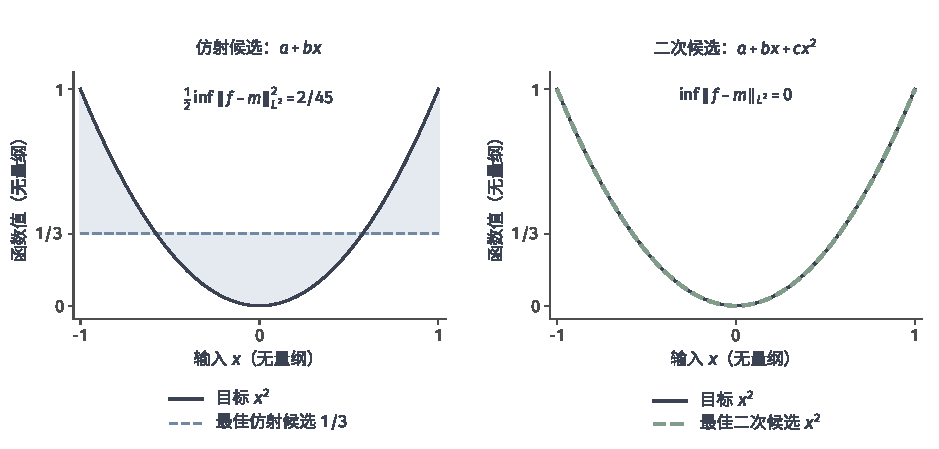
\includegraphics[width=159mm]{figures/04-classic-models/00-shared/matplotlib/regression-feature-approximation/figure.pdf}
  \caption{固定目标$m(x)=x^2$与不同候选空间的最佳逼近。输入在$[-1,1]$上均匀分布；左图中，所有仿射函数的最佳候选为$1/3$，阴影表示它与目标的差距，平方距离的一半为$2/45$。右图加入二次特征后，候选空间包含目标，最小距离为零。图中比较的是候选空间，不使用训练样本。}
  \label{fig:regression-feature-approximation}
\end{figure*}

选择新的特征向量$\bm\phi(\bm x)$以后，模型仍对系数线性，学习仍使用同一个最小二乘目标，改变的是设计矩阵的列。多项式使用$1,x,\ldots,x^q$；径向基$\exp(-(x-c_j)^2/(2s^2))$在中心$c_j$附近产生局部起伏，$s>0$决定作用范围。固定中心与尺度后，只需学习各基函数的加权系数；若也要选择这些位置与尺度，应在训练折内完成并用验证误差比较。

样条用分段多项式描述局部变化，并约束相邻段如何连接。结点$\xi_1,\ldots,\xi_K$是分段接合的位置。三次样条要求函数值和前两阶导数在结点两侧连续，可以用$1,x,x^2,x^3$及$(x-\xi_k)_+^3$展开，其中$(a)_+=\max(a,0)$。全局三次项给出左侧起始曲线，截断项从各自结点起改变右侧形状；它在结点处的函数值和前两阶导数都为零，因而保留接合条件。只用截断项会遗漏一般的全局多项式部分。

增加基函数能提供新的曲线形状，也会增加待估系数并可能加重共线性。下面先看观测误差结构与异常响应怎样改变拟合，再用正则化控制系数。核方法则把显式特征的内积换为核值计算，相关回归形式见第\ref{sec:regression-kernel-svr}节\scite{hastie2009}。

\subsubsection{观测精度与异常响应}

\paragraph{利用观测误差结构}
\label{sec:regression-weighted-noise}

观测精度不同，平方残差也未必应受到相同权重。假设两次独立观测测量同一个未知常数，噪声方差分别为$1$和$100$。OLS直接取两次观测的平均；用噪声方差倒数加权，则给第一条观测$100$倍于第二条的权重，降低较不精确观测的影响。

更一般地，已知正定误差协方差$\bm\Omega$时，最小化$(\bm y-\bm X\bm w)^\top\bm\Omega^{-1}(\bm y-\bm X\bm w)$得到\term{广义最小二乘}（generalized least squares, GLS）。它按噪声结构重新度量残差，对角$\bm\Omega$对应加权最小二乘，用$\bm\Omega^{-1/2}$变换数据即可回到同方差问题。异方差在零条件均值下不破坏OLS无偏性，却会改变其协方差，因此这种调整服务于估计方差；若$\bm\Omega$也要由样本估计，还要计入协方差估计的误差。

这个变换必须同时施于响应与全部特征。取对称正定逆平方根$\bm C=\bm\Omega^{-1/2}$，令$\bm y'=\bm C\bm y$、$\bm X'=\bm C\bm X$，就把观测方程变成$\bm y'=\bm X'\bm w+\bm C\bm\varepsilon$。新误差的协方差为$\bm C\bm\Omega\bm C^\top=\bm I_n$，因此这种消除噪声尺度与相关性的操作称为白化（whitening）。变换后的普通残差平方和$\lVert\bm y'-\bm X'\bm w\rVert_2^2$恰好等于原来的协方差加权目标。对角$\bm\Omega$只要求把第$i$条记录的响应与每个特征一起除以其误差标准差；非对角时还会混合不同记录，从而消除误差相关。随后对$(\bm X',\bm y')$使用前述QR或SVD求系数，再在原特征上计算$\bm\phi(\bm x)^\top\bm w$；白化改变了训练准则，并未改变新输入的预测公式。

\paragraph{限制异常响应的影响}
\label{sec:regression-huber}

如果少数响应记录受到污染，而预测仍面向未受污染的数据，追随这些记录就可能把拟合偏离真正的预测目标。限制污染记录的影响是改善泛化的一条思路；若极端响应本来就是目标分布的一部分，则还需检查这种限制是否符合所用损失和预测目标。

平方损失把十倍残差变成一百倍损失，少量错误记录因此可能主导拟合。只拟合一个常数时，构造响应$(0,0,0,20)$的OLS预测为$5$；最后一个大响应把预测从前三个样本所在的零点拉开。若希望保留小误差处的平滑拟合，又减轻大残差的作用，可以让损失在离零较远处按残差绝对值增长。

\term{Huber损失}（Huber loss）采用这一做法：小残差处保持二次形状，大残差处改为线性增长，从而限制残差方向的导数。取下式阈值$\delta=1$，刚才四个响应的最优常数变成$1/3$；三个小残差共同抵消最后一个被截断的残差导数。它来自稳健位置估计的研究，也可用于回归目标\scite{huber1964}。
\begin{equation}
  \rho_\delta(r)=
  \begin{cases}
    r^2/2,&|r|\leq\delta,\\
    \delta|r|-\delta^2/2,&|r|>\delta,
  \end{cases}
  \qquad\delta>0.
  \label{eq:regression-huber-loss}
\end{equation}
对$r_i=y_i-\bm{\phi}(\bm{x}_i)^{\top}\bm{w}$最小化$\sum_i\rho_\delta(r_i)$，估计方程为$\sum_i\bm{\phi}(\bm{x}_i)\psi_\delta(r_i)=\bm{0}$，其中$\psi_\delta(r)=\max(-\delta,\min(r,\delta))$。令$a_i=\min(1,\delta/|r_i|)$，在$r_i=0$时取$a_i=1$，便可交替计算残差权重与加权最小二乘；应检查目标和估计方程的收敛。阈值$\delta$具有响应单位，常结合稳健尺度估计选择；采用中位绝对偏差定标时，还需按误差分布校准所用倍数。

这个权重使$\psi_\delta(r_i)=a_i r_i$。具体求解时，从当前系数算出残差，再由这些残差算出$a_i$；本轮暂时固定权重，最小化$\sum_i a_i(y_i-\bm\phi(\bm x_i)^\top\bm w)^2$，其正规方程就使用加权残差$a_i r_i$。新系数会改变残差和权重，因此必须重新计算并重复，这就是反复加权最小二乘（iteratively reweighted least squares，IRLS）的闭环，不能只用一次OLS残差定权后便当作Huber解。停止时还要核对原Huber目标和原估计方程，而不只比较两轮系数的变化。

前面的常数算例也可在这个方程中复算。设常数预测为$a$，$\delta=1$；在$0\leq a\leq1$内，三个零响应的残差导数都是$-a$，响应$20$的残差导数则为$1$，所以估计方程为$-3a+1=0$，给出$a=1/3$。它确实落在所用分段内，凸性保证该驻点为全局最小点。用于选择阈值的中位绝对偏差（median absolute deviation，MAD）则是$\operatorname{median}_i|r_i-\operatorname{median}_j r_j|$；它给出稳健的残差尺度，不能替代阈值在目标误差分布下的校准。

将一般残差函数$\rho$代入$\min_{\bm{w}}\sum_i\rho(r_i)$，便得到以回归参数为目标的\(M\)估计（M-estimation）。Huber准则凸且连续可微；Tukey双权、Cauchy等准则则可能非凸，求解与统计性质须分别分析。估计方程中的样本贡献是特征向量与$\psi_\delta$的乘积。有界残差导数限制了响应方向的影响，但远离其他输入的高杠杆点仍可因特征幅度较大而主导估计。Huber准则拟合的是自身损失下的最优中心；条件分布偏斜时，令截断残差导数平均为零所得到的中心可能偏离条件均值。因此应按Huber损失及任务需要验证预测，不能将残差降权直接当成条件均值平方风险的改善保证。

\subsection{正则化线性回归}
\label{sec:regression-regularization}

面积与套内面积高度相关时，许多系数组合能产生近似相同的训练预测，数据却难以分辨它们。把情形简化为两列特征完全相同，预测就只取决于$w_1+w_2$；$(100,-98)$与$(1,1)$在训练点上给出同样结果。到了两列略有差别的新输入$(1.01,1)$，两组系数的预测却分别为$3$与$2.01$。较大的相反系数把训练中几乎看不到的差异放大了。

\term{正则化}（regularization）在拟合准则中加入参数约束或惩罚，让这种缺少数据支持的变化也付出代价。直观地说，在训练集上几乎无法区分的两组系数，我们倾向于选数值更小、更“不极端”的那一组，因为大的相反系数相当于在数据很少看到的方向上押了重注，新样本稍有不同就会被放大成预测剧变。它可以减少估计的波动，但系数被压小也可能连带压低真实信号。因此，正则化的用途是用可接受的偏差换取较小的方差，是否改善未来预测仍取决于真实结构、正则强度和测试分布。

\subsubsection{模型结构}
\label{sec:regression-penalties}

本小节将截距$b$与斜率$\bm{w}\in\mathbb{R}^d$分开。平方损失下，固定斜率的最优截距为$b=\bar y-\bar{\bm{x}}^{\top}\bm{w}$，所以可先用训练均值中心化特征与响应，只优化斜率，再恢复截距。以下$\bm{X},\bm{y}$均指中心化后的量，截距不受惩罚；需要标准化时，尺度也只能从训练集估计。

四种常见方法都在$\lVert\bm{y}-\bm{X}\bm{w}\rVert_2^2/(2n)$之外增加凸惩罚。\term{岭回归}（ridge regression）使用$\lambda\lVert\bm{w}\rVert_2^2/2$抑制参数幅度，收缩数据约束较弱的方向。Hoerl与Kennard在1970年的论文中系统研究了非正交设计下的有偏估计：当共线性使OLS方差过大时，容许一定偏差可能换来较小的均方误差\scite{hoerl1970ridge}。

岭回归通常保留每个变量，只把系数变小。如果记录了许多特征，而我们还希望删去缺乏预测作用的坐标，就需要让某些系数恰好为零。\term{Lasso}（least absolute shrinkage and selection operator）使用$\lambda\lVert\bm w\rVert_1$实现这种选择。绝对值惩罚在零点有尖点，损失项对某个坐标的推动较弱时，最优系数可以停在零点。比如正交标准化设计下，OLS系数为$(0.12,1.40)$，取$\lambda=0.20$后Lasso得到$(0,1.20)$；岭回归在同一数值的惩罚系数下则得到$(0.10,1.40/1.20)$，两个坐标都保留。这里比较的是两种惩罚的作用方式，不代表相同数值的$\lambda$给出相同强度的约束。Tibshirani在1996年提出Lasso，将连续收缩与变量选择放进同一个优化问题\scite{tibshirani1996lasso}。

这个教学设计的“正交标准化”具体指中心化后$\bm X^\top\bm X/n=\bm I_d$：不同列的样本内积为零，每列平方长度为$n$。于是每个坐标都有相同的数据曲率，坐标之间没有交叉项；Lasso分别将OLS系数向零移动$\lambda$并截断，岭回归则分别除以$1+\lambda$。上面的数值由这两种操作直接得到；后面将从最优性条件说明软阈值的来由。

Lasso的坐标选择在特征高度相关时也会出现歧义。若两列完全相同，并且最优系数和为正，$(a,0)$、$(0,a)$与$(a/2,a/2)$具有同样的数据拟合和一范数惩罚。数据难以决定该保留哪个变量，轻微扰动就可能改变选择。\term{弹性网}（elastic net）在一范数之外加入二次惩罚；上面三种分配中，平均分摊的平方范数最小。它因此同时保留坐标选择和稳定相关系数的机制。惩罚写成$\lambda_1\lVert\bm w\rVert_1+\lambda_2\lVert\bm w\rVert_2^2/2$，常取$\lambda_1=\lambda\alpha$、$\lambda_2=\lambda(1-\alpha)$，其中$0\leq\alpha\leq1$。Zou与Hastie在2005年研究了这一结合；原始文献还讨论了对系数重标定以修正过度收缩的版本\scite{zou2005elastic}。

另一些变量由多个系数共同表示。例如用$t,t^2,t^3$表示楼龄作用，三个坐标合起来才是一个楼龄函数；我们的选择问题可能是“是否保留楼龄”，而不是“是否保留某次幂”。\term{组Lasso}（group Lasso）把预先指定的一组坐标作为一个选择单位，使用惩罚$\lambda\sum_{g=1}^{G}\omega_g\lVert\bm w_{A_g}\rVert_2$。其中$A_1,\ldots,A_G$是不重叠且覆盖全部斜率坐标的组，$\omega_g>0$为组权重，常取$\sqrt{|A_g|}$。组向量为零，就意味着这一整组的作用被删除；保留一组则允许各系数共同拟合其形状，组内的某些坐标仍可为零。Yuan与Lin在2006年研究了这种成组变量选择，包括分类特征展开的多个指示变量\scite{yuan2006group}。

表\ref{tab:regression-regularization-comparison}将四种方法放在相同的平方损失下比较。选择方法时，需要区分“系数整体变小”“某个坐标变零”和“某组变量一起变零”；这三种要求对应不同的结构假设。

\begin{table*}[t]
  \centering
  \small
  \setlength{\tabcolsep}{4pt}
  \renewcommand{\arraystretch}{1.25}
  \begin{tabularx}{\linewidth}{@{}>{\RaggedRight\arraybackslash}p{16mm}>{\RaggedRight\arraybackslash}p{42mm}>{\RaggedRight\arraybackslash}p{24mm}>{\RaggedRight\arraybackslash}p{34mm}>{\RaggedRight\arraybackslash}X@{}}
    \toprule
    方法 & 惩罚项 & 稀疏形式 & 相关特征与解 & 适用考虑 \\
    \midrule
    岭回归 & $\lambda\lVert\bm{w}\rVert_2^2/2$ & 通常不产生零系数 & 分摊相关特征贡献；$\lambda>0$时解唯一 & 多个弱效应、共线性；重点在稳定预测 \\
    \addlinespace
    Lasso & $\lambda\lVert\bm{w}\rVert_1$ & 单坐标稀疏 & 可能在相关变量间选择；解未必唯一 & 少数变量有效；需检查选择的稳定性 \\
    \addlinespace
    弹性网 & $\lambda_1\lVert\bm{w}\rVert_1$\newline ${}+\lambda_2\lVert\bm{w}\rVert_2^2/2$ & $\lambda_1>0$时可坐标稀疏 & 二次项促进相近特征的系数接近；$\lambda_2>0$时解唯一 & 同时需要变量选择与相关特征的稳定估计 \\
    \addlinespace
    组Lasso & $\lambda\sum_g\omega_g\lVert\bm{w}_{A_g}\rVert_2$ & 整组稀疏；组内未必稀疏 & 组须预先给定；解未必唯一 & 指示变量、基函数等具有已知分组的特征 \\
    \bottomrule
  \end{tabularx}
  \caption{正则化线性回归的比较。共同数据项为$\lVert\bm{y}-\bm{X}\bm{w}\rVert_2^2/(2n)$，截距不受惩罚；组Lasso采用不重叠分组。稀疏性表示惩罚允许出现的结构，并不保证任意数据和正则强度都产生零系数。特征尺度与超参数仍须在训练集内确定。}
  \label{tab:regression-regularization-comparison}
\end{table*}

图\ref{fig:regression-regularization-geometry}进一步用二维约束说明差别。对给定约束半径，从无约束最优点向外扩张等损失线，第一次接触可行域的位置就是约束最优解。一范数球在坐标轴上有尖点，因此接触点可能恰好有零坐标；二范数球的边界光滑，通常只连续收缩系数。这个几何图解释了稀疏解为何可能出现，严格判断仍应回到最优性条件。

\begin{figure*}[t]
  \centering
  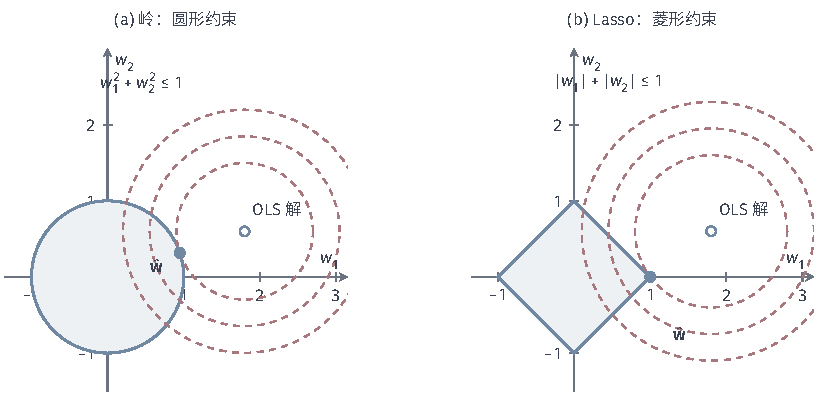
\includegraphics[width=138.649mm]{figures/04-classic-models/00-shared/tikz/regression-regularization-geometry/figure.pdf}
  \caption{岭与Lasso的约束几何。构造损失为$J(\bm{w})=\lVert\bm{w}-(1.8,0.6)^{\top}\rVert_2^2/2$，虚线为等损失线，浅色区域为可行域，空心点为OLS解，实心点为约束最优解。左图解为$(1.8,0.6)^{\top}/\sqrt{3.6}$，右图解为$(1,0)^{\top}$。两图都取单位约束半径以比较形状，不表示相同的惩罚强度；Lasso也并非总在尖点取到最优解。}
  \label{fig:regression-regularization-geometry}
\end{figure*}

岭惩罚沿设计矩阵的谱方向收缩系数，一般设计下各原始坐标受到的相对收缩可以不同，下面将给出相应分解。惩罚的概率解释同样依赖归一化：高斯似然下，高斯先验对应二次惩罚，各系数独立的拉普拉斯先验（Laplace prior）对应一范数惩罚，但先验尺度与$\lambda$的对应关系还包含$n$和噪声方差。

\subsubsection{参数学习}
\label{sec:regression-regularization-learning}

岭回归仍有直接求解与迭代求解两条路线。先把平方损失与二次惩罚相加，再对系数求导。令梯度$\bm X^\top(\bm X\bm w-\bm y)/n+\lambda\bm w$为零，便得到一个在OLS正规方程上增加$n\lambda\bm I$的线性系统；其解为
\begin{equation}
  \widehat{\bm{w}}_{\lambda}
  =(\bm{X}^{\top}\bm{X}+n\lambda\bm{I})^{-1}\bm{X}^{\top}\bm{y},
  \qquad\lambda>0.
  \label{eq:regression-ridge-solution}
\end{equation}
任意非零$\bm{v}$满足$\bm{v}^{\top}(\bm{X}^{\top}\bm{X}+n\lambda\bm{I})\bm{v}=\lVert\bm{X}\bm{v}\rVert_2^2+n\lambda\lVert\bm{v}\rVert_2^2>0$，所以即使设计秩亏，斜率解也唯一。若$\gamma_{\max},\gamma_{\min}$是$\bm{X}^{\top}\bm{X}$的极端特征值，正则化后该矩阵的条件数为$(\gamma_{\max}+n\lambda)/(\gamma_{\min}+n\lambda)$；比较对象是正规方程矩阵，而非$\bm{X}$本身的条件数。

取$\bm{X}=\bm{U}_r\bm{D}_r\bm{V}_r^{\top}$，正奇异值为$s_j$，则
\begin{equation}
  \bm{X}\widehat{\bm{w}}_{\lambda}
  =\sum_{j=1}^{r}\frac{s_j^2}{s_j^2+n\lambda}
       \bm{u}_j\bm{u}_j^{\top}\bm{y}.
  \label{eq:regression-ridge-spectral}
\end{equation}
OLS保留列空间中的全部投影，岭回归则按$s_j^2/(s_j^2+n\lambda)$保留各方向，小奇异值方向受到更强收缩。这是稳定性改善的来源，也说明惩罚会同时压低这些方向上的真实信号。

这一分解可由前面介绍的SVD直接算出。沿$\bm v_j$方向，$\bm X^\top\bm X+n\lambda\bm I$的特征值为$s_j^2+n\lambda$，而$\bm X^\top\bm y$在该方向的分量为$s_j\bm u_j^\top\bm y$。因此岭系数在此方向等于$s_j\bm u_j^\top\bm y/(s_j^2+n\lambda)$；再乘$\bm X$产生训练预测时，多出一个$s_j$，就得到式\eqref{eq:regression-ridge-spectral}的因子。$\bm X$零空间中的右端分量为零，岭解在这些方向也取零。这里的$\bm u_j$仍是$n$维训练预测方向，并不是原始输入坐标。

Lasso的目标记为$F(\bm{w})$。由于$\lambda>0$时$F(\bm{w})\geq\lambda\lVert\bm{w}\rVert_1$，连续目标至少取得一个最小值；参数解未必唯一。要理解零系数为何可能最优，可以先固定其他坐标。令$\bm{r}_{-j}=\bm{y}-\sum_{k\ne j}\bm{X}_{:,k}w_k$，$a_j=\lVert\bm{X}_{:,j}\rVert_2^2/n$、$c_j=\bm{X}_{:,j}^{\top}\bm{r}_{-j}/n$，略去常数后的单坐标目标为
\[
  q_j(w_j)=\frac{a_j}{2}w_j^2-c_jw_j+\lambda|w_j|.
\]
在零点左侧，绝对值项的斜率为$-\lambda$；右侧则为$\lambda$。因此零点的左右导数分别为
\[
  q'_{j,-}(0)=-c_j-\lambda,\qquad
  q'_{j,+}(0)=-c_j+\lambda.
\]
这个目标是凸函数，零点最优恰好要求左导数不大于零、右导数不小于零，即$|c_j|\leq\lambda$。此时无论向哪一侧离开零点，目标都不会降低；损失项在零点的导数$-c_j$却不必为零。

刚才的零系数虽然已经最优，损失项的导数却不一定为零，而绝对值惩罚在零点又没有普通导数。因此，OLS使用的“总梯度等于零”不能直接检验这个解。我们需要一种允许惩罚在零点提供一段斜率、并检验这些斜率能否抵消损失导数的条件。

\term{次梯度}（subgradient）用位于凸函数下方的支持直线描述这些可用斜率。对一维凸函数$f$，若斜率$s$满足$f(v)\geq f(u)+s(v-u)$对所有$v$成立，它就是$f$在$u$处的一个次梯度：经过该点、斜率为$s$的直线始终位于函数图像下方。所有这样的斜率组成次梯度集合$\partial f(u)$；可导时集合只有导数一个元素，而$|u|$在零点允许$[-1,1]$中的全部斜率。

凸函数的最优性因而可统一表为$0\in\partial f(u)$。对Lasso，损失梯度加上惩罚次梯度为零，得到充要最优性条件
\begin{equation}
  \frac{\bm{X}^{\top}(\bm{y}-\bm{X}\widehat{\bm{w}})}{n}
  =\lambda\bm{z},\qquad
  z_j\in
  \begin{cases}
    \{\operatorname{sign}(\widehat w_j)\},&\widehat w_j\ne0,\\
    [-1,1],&\widehat w_j=0.
  \end{cases}
  \label{eq:regression-lasso-kkt}
\end{equation}
其中非零坐标对应的绝对值导数为符号函数，零坐标则允许整个区间来抵消损失梯度。沿用上述$a_j,c_j$，在正、负半轴求导，并在零点检验$|c_j|\leq\lambda$，得到坐标更新
\begin{equation}
  w_j\leftarrow\frac{\mathcal{S}_{\lambda}(c_j)}{a_j},
  \qquad
  \mathcal{S}_{\lambda}(c)=\operatorname{sign}(c)(|c|-\lambda)_+.
  \label{eq:regression-soft-threshold}
\end{equation}
这里$a_j>0$，零列直接取零系数。\term{软阈值}（soft thresholding）把阈值内的量置零，将其余量向零移动$\lambda$。例如正交标准化设计下，OLS系数$(0.12,1.40)$在$\lambda=0.20$时变为$(0,1.20)$；相关设计则需反复更新部分残差，不能直接阈值化OLS系数。循环坐标下降可用式\eqref{eq:regression-lasso-kkt}的违反程度作为停止依据。

回到前面的正交例子，此时$a_j=1$，其他列与第$j$列正交，因而$c_j=\bm X_{:,j}^\top\bm y/n$不随其他坐标的更新改变，恰好就是该坐标的OLS系数。这说明何以能够一次对OLS系数应用阈值。一般相关设计没有这个消去交叉项的条件，所以每次更改一个坐标后，其余坐标的部分残差也必须跟着更新。

弹性网的坐标更新为$\mathcal{S}_{\lambda_1}(c_j)/(a_j+\lambda_2)$。

组惩罚需要对整段系数共同作取舍。记光滑数据项为$g(\bm w)=\lVert\bm y-\bm X\bm w\rVert_2^2/(2n)$，把惩罚另记为$\operatorname{pen}(\bm w)$。数据项处处可微，一范数与组范数却在零点有尖点，不能简单套用“求梯度再沿负方向走一步”；而且组Lasso的最小单位是一整组系数，逐坐标更新无法判断整组是否该一起置零。近端梯度（proximal gradient）专为“光滑项＋带尖角的凸惩罚”这种组合设计：先用一条简单的二次函数在当前点附近从上方近似光滑的数据项，把“向数据更吻合的方向走一步”与“缩小惩罚”合并成一个通常有闭式答案的子问题。非零设计下，令$L=\lVert\bm X^\top\bm X/n\rVert_2$，取$0<t\leq1/L$，则
\[
 \begin{aligned}
 g(\bm u)&\leq g(\bm w)+\nabla g(\bm w)^\top(\bm u-\bm w)\\
 &\qquad+\frac{1}{2t}\lVert\bm u-\bm w\rVert_2^2.
 \end{aligned}
\]
把右侧与原惩罚相加，再对二次项配方，就得到$\min_{\bm u}\lVert\bm u-\bm v\rVert_2^2/2+t\operatorname{pen}(\bm u)$，其中$\bm v=\bm w-t\nabla g(\bm w)$。这个子问题在“靠近数据项的梯度步”与“减小惩罚”之间作取舍；由于原惩罚没有被求导，零点的尖角及选择作用仍然保留。不重叠组的平方距离与惩罚都能按组相加，所以这个子问题可以分组求解。

组惩罚则可用近端梯度：先令$\bm{v}=\bm{w}-t\bm{X}^{\top}(\bm{X}\bm{w}-\bm{y})/n$，再逐组计算
\begin{equation}
  \bm{w}_{A_g}^{+}
  =
  \begin{cases}
    \bm{0},&\lVert\bm{v}_{A_g}\rVert_2\leq t\lambda\omega_g,\\
    \left(1-\dfrac{t\lambda\omega_g}{\lVert\bm{v}_{A_g}\rVert_2}\right)
      \bm{v}_{A_g},&\text{其他情形}.
  \end{cases}
  \label{eq:regression-group-prox}
\end{equation}
该式求解的是$\min_{\bm{u}}\lVert\bm{u}-\bm{v}_{A_g}\rVert_2^2/2+t\lambda\omega_g\lVert\bm{u}\rVert_2$：固定$\lVert\bm{u}\rVert_2$时，同向选择使平方距离最小，剩下的一维非负半轴问题给出径向阈值。该闭式解针对欧氏距离构成的近端子问题；一般设计的块坐标子问题还包含组内设计的曲率，需要据此求解。对非零设计，取$0<t\leq1/\lVert\bm{X}^{\top}\bm{X}/n\rVert_2$可保证凸近端梯度法的目标收敛性质。

具体地，当$\bm v_{A_g}\ne\bm0$时，把同向候选写成$\bm u=r\bm v_{A_g}/\lVert\bm v_{A_g}\rVert_2$，其中$r\geq0$。要最小化的标量目标就是
\[
 \frac12(r-\lVert\bm v_{A_g}\rVert_2)^2
       +t\lambda\omega_g r,\qquad r\geq0.
\]
其内部驻点为$r=\lVert\bm v_{A_g}\rVert_2-t\lambda\omega_g$；若这个值为负，约束最小点就在$r=0$。合起来即$r=(\lVert\bm v_{A_g}\rVert_2-t\lambda\omega_g)_+$，代回同向候选就得到组阈值公式。$\bm v_{A_g}=\bm0$时直接取零，不需要作除法。

沿$\lambda$网格使用前一个解热启动，可以减少重复计算。LARS的Lasso修正版利用分段线性路径求解一范数惩罚问题，但这一性质不直接推广到一般Group Lasso。超参数通常由交叉验证选择；中心化、标准化与变量选择都必须在每个训练折内完成。跨软件比较超参数时，应先将平方损失与惩罚换算到相同的系数约定\scite{hastie2009}。

这里的LARS指最小角回归（least angle regression）算法。理解上述路径只需抓住一段局部机制：在活跃列线性独立、非零坐标及其符号保持不变的一段上，Lasso最优性方程是关于这些系数的线性系统，右端随$\lambda$作线性变化，所以解也随$\lambda$作线性变化。变量进入、退出或符号改变时，进入另一段；LARS的修正版据此追踪路径。这项说明不把所有组范数惩罚都视为同样的折线。

\subsubsection{收缩的收益与变量选择的边界}
\label{sec:regression-regularization-theory}
\label{sec:regression-elastic-net}
\label{sec:regression-group-lasso}

正则化没有自动增加特征中缺少的函数。有限惩罚改变的是从原有系数中怎样取舍；硬约束才会直接排除范围外的候选。岭的谱因子显示，小奇异值方向的噪声与真实信号都会被压低，所以稳定系数要付出偏差代价。

正则化用偏差换方差，值得把这两个词讲具体。模型是在一个有限训练集上训练出来的：如果同样的数据生成过程重新抽样，得到一批新的训练记录，再用完全相同的方法训练，新模型的预测通常会和旧模型略有不同。所谓方差，就是预测在这种“换一批训练集”的重复实验中围绕自身平均值的摆动；所谓偏差，是这些预测的平均值与真实条件均值之间的固定差距。固定未来输入$\bm x$，设其响应均值为$m(\bm x)$，未来噪声独立于训练记录且方差有限。把由不同训练集得到的预测再取平均，平方误差便分解为
\[
 \begin{aligned}
 \mathbb E[(Y_\star-\widehat f(\bm x))^2\mid\bm x]
 &=\operatorname{Var}(Y_\star\mid\bm x)\\
 &\quad+[\mathbb E\widehat f(\bm x)-m(\bm x)]^2\\
 &\quad+\operatorname{Var}(\widehat f(\bm x)).
 \end{aligned}
\]
把误差拆成未来噪声、平均预测偏离真实均值、以及预测围绕其平均的波动，展开平方后交叉项的期望为零，就得到这三项。惩罚可能降低最后一项，同时增大中间一项；是否有益要比较两者之和。图\ref{fig:regression-bias-variance-noise}给出这种取舍的示意，不是对任意数据的性能排序。

\begin{figure}[htbp]
  \centering
  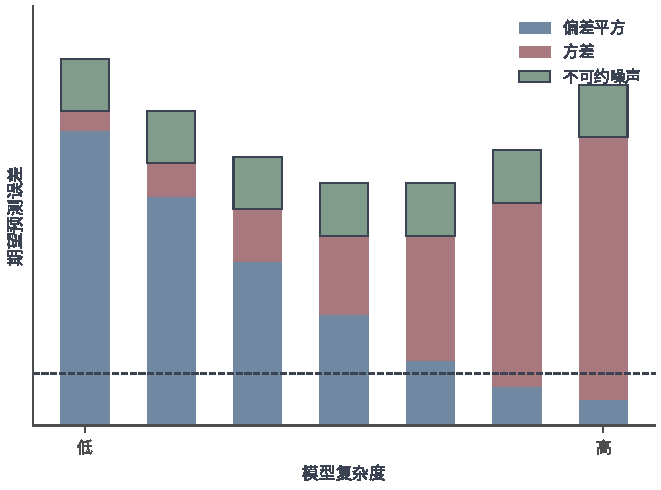
\includegraphics[width=105.412mm]{figures/04-classic-models/00-shared/matplotlib/regression-bias-variance-noise/figure.pdf}
  \caption{模型复杂度变化时的偏差—方差—噪声分解示意。柱高是教学构造的相对量，不来自实验：复杂度增加时偏差平方下降、估计方差上升，不可约噪声保持不变。总误差由三部分共同决定，因此“模型更复杂”与“误差更小”都不是无条件结论。}
  \label{fig:regression-bias-variance-noise}
\end{figure}

变量选择还要区分“预测准确”与“识别真实变量”。两个高度相关变量可能互相替代，预测仍然接近，选中哪个却会随样本变化。弹性网的正二次惩罚使解唯一；两列完全相同时，交换系数不改变目标，唯一性便要求它们相等。组Lasso则按预定组共同取舍，不能据此保证组内每个坐标都非零。若希望同时选择组与组内坐标，可以在组惩罚之外再加$\lambda_1\lVert\bm w\rVert_1$，得到\term{稀疏组Lasso}（sparse group Lasso）；对互不重叠的组，学习时先对梯度步作阈值$t\lambda_1$的坐标软阈值，再按组作阈值$t\lambda\omega_g$的径向阈值，正则强度仍由训练内验证选择。

\subsubsection{成分回归：PCR与PLS}

\label{sec:regression-component-regression}

处理共线性的另一条路线不是给系数加惩罚，而是先对输入本身做一次“改换坐标系”的预处理：把众多彼此相关的原始变量合成为少数几个互不相关的综合指标（成分），再在这些成分上做回归。由于成分数量少且相互正交，在它们上面估计系数就避开了“两列几乎相同、系数无法分辨”的问题；代价是必须决定保留多少、保留哪些成分。\term{主成分回归}（principal component regression, PCR）保留若干主成分，在这些正交方向上拟合，等价于对选中方向完全保留、对其余方向硬截断。第\ref{sec:dim-pca}节从无监督表示的角度推导主成分分析（PCA）：PCA与PCR共享由输入方差确定的主成分基，但PCA按方差保留与重构误差评价表示，PCR还要用响应检验这些成分是否有利于预测。与式\eqref{eq:regression-ridge-spectral}的连续收缩相比，PCR的取舍更直接，但输入方差小不意味着对响应不重要。\term{偏最小二乘回归}（partial least squares regression, PLS）在构造成分时同时利用输入与响应的关系，因而属于监督降维；它有不同的具体算法，不能笼统理解为收缩因子必在$0$和$1$之间的岭回归。

以一种常见的单响应线性PLS构造为例，先将输入与响应中心化，把总体随机输入向量另记为$\bm Z=(X_1,\ldots,X_d)^\top$。在单位系数方向$\lVert\bm a\rVert_2=1$中寻找成分$T=\bm a^\top\bm Z$，使$\operatorname{Cov}(T,Y)^2$最大；训练时用样本协方差代替总体协方差，仍由设计矩阵$\bm X$得到样本成分向量$\bm t=\bm X\bm a$。单位长度约束防止仅靠放大系数无限增大协方差，使用响应协方差则使方向选择面向预测。后续成分在已解释部分移除后继续提取信息，并满足所用算法的正交要求；具体消去方式随PLS算法而异。

例如教学构造中，$X_1,X_2$独立、方差分别为$100$与$1$，响应为$Y=X_2$。不额外标准化时，PCA的第一主成分为$X_1$；只保留这一成分做PCR会丢掉全部响应信号。PLS构造成分时利用输入与响应的关系，在这个例子中可以识别$X_2$与$Y$的关联，而不只按输入方差决定取舍。成分数同样需要在训练折内选择。

刚才的教学分布给出$\operatorname{Cov}(X_1,Y)=0$、$\operatorname{Cov}(X_2,Y)=1$，所以$\operatorname{Cov}(a_1X_1+a_2X_2,Y)=a_2$。在$a_1^2+a_2^2=1$下，协方差平方在$a_1=0$、$|a_2|=1$时最大，即选中$X_2$方向；PCA的方差准则则选中$X_1$方向。这个计算只比较两种方法怎样选第一成分，不声称有限样本总能准确识别信号，也不替代成分数的训练折内选择。

选出成分还没有完成回归。把训练得到的线性变换记为$\bm R\in\mathbb R^{d\times m}$，成分设计为$\bm T=\bm X\bm R$；PCR取选中的主成分方向，PLS则使用其训练算法给出的成分变换。接着拟合
\[
 \begin{aligned}
 \widehat{\bm\gamma}&\in\argmin_{\bm\gamma}
       \|\bm y-\bm T\bm\gamma\|_2^2,\\
 \widehat f(\bm x)&=\bar y+
       (\bm x-\bar{\bm x})^\top\bm R\widehat{\bm\gamma}.
 \end{aligned}
\]
这里$\bm X,\bm y$已中心化，$\bar{\bm x},\bar y$来自该训练折；若还做标准化，新输入也要用同一尺度。使用PLS时，新输入必须经过训练中固定下来的同一套成分变换，不能重新按新响应选择方向。最后由验证比较成分数，既不能只保留方差最大的方向就结束，也不能只计算协方差方向而省略响应系数的学习\scite{hastie2009}。

\label{sec:regression-regularization-summary}
惩罚约束原坐标中的系数，PCR与PLS先改变回归使用的方向；两条路线都需在验证中决定保留多少信息。尺度处理、成分提取与变量选择必须跟随每个训练折重新完成。

\subsection{分位数回归（Quantile Regression）}
\label{sec:regression-quantiles}

预算制定者关心的是实际支出超过预算的概率，单个条件均值无法回答这个问题。假设同类任务的支出以$80\%$概率为$100$，以$20\%$概率为$200$。平均支出是$120$，照此准备预算仍有$20\%$概率超支；如果要求至少$90\%$的支出不超过预算，这个例子中应把阈值提高到$200$。两种预测使用同一响应分布，差别来自需要完成的决策。\term{分位数回归}（quantile regression）用非对称残差损失估计给定输入后的指定分位数；例如$0.9$分位数提供一个使响应至少有$90\%$概率不超过它的条件阈值。Koenker与Bassett在1978年系统提出回归分位数，将回归目标从条件均值扩展到条件分布的不同位置。这一区分源于决策目标，无需先假定误差对称或同方差\scite{koenker1978quantiles}。

\subsubsection{模型结构}

预算阈值低估时产生超支，高估时则预留过多；两种偏差的代价可以不同，而平方损失对高估和低估一视同仁，无法表达这种不对称。要估计某个分位数，就要让落在阈值两侧的误差按不同的权重计分：估低了（实际值高于预测）更接近我们想避免的超支，就给更高的权重。给定$0<\tau<1$，\term{分位数损失}（pinball loss）用$\tau$和$1-\tau$分别给正、负残差计分：
\begin{equation}
  \rho_\tau(r)=
  \begin{cases}
    \tau r,&r\geq0,\\
    (1-\tau)(-r),&r<0.
  \end{cases}
  \label{eq:regression-pinball}
\end{equation}
残差仍取$r=y-\widehat y$，所以较大的$\tau$更重地惩罚低估。线性分位数回归最小化$\sum_i\rho_\tau(y_i-\bm\phi(\bm x_i)^\top\bm w)$。要说明这种非对称计分为什么选择分位数，可以先只预测一个常数$a$。对前面固定的$0<\tau<1$，假设$\mathbb E|Y|<\infty$，记响应分布函数为$F_Y$，期望损失为$Q(a)=\mathbb E[\rho_\tau(Y-a)]$。

我们比较把$a$提高一点以后，损失怎样改变。若$Y<a$，这次调整加重高估，单位变化的代价为$1-\tau$；若$Y>a$，调整减轻低估，单位变化的损失减少$\tau$。当响应恰好等于$a$时，向左、向右的变化率不同，所以要分别计算单侧导数。单条损失的变化率始终有界，因而可以在期望内取相应单侧极限，得到
\begin{equation}
 \begin{aligned}
  Q'_-(a)&=(1-\tau)\mathbb P(Y<a)
            -\tau\mathbb P(Y\geq a)\\
          &=F_Y(a-)-\tau,\\
  Q'_+(a)&=(1-\tau)\mathbb P(Y\leq a)
            -\tau\mathbb P(Y>a)\\
          &=F_Y(a)-\tau.
 \end{aligned}
 \label{eq:regression-pinball-one-sided}
\end{equation}
$Q$是凸函数，最优点要求左导数不大于零、右导数不小于零；因此，它的全部最小点恰好满足
\[
 F_Y(a-)\leq\tau\leq F_Y(a),
 \qquad F_Y(a-)=\mathbb P(Y<a).
\]
这两条不等式同时处理了响应在某一点具有正概率的情形，以及分布函数在一段区间上保持不变的情形；它们保留了可能不唯一的最优点集合。以刚才两种支出为例，$\tau=0.9$、$a=200$时，左、右导数分别为$0.8-0.9=-0.1$和$1-0.9=0.1$，向任一侧移动都不能降低期望损失。若改取$\tau=0.8$，则$[100,200]$中的每个阈值都满足上述条件，整个区间的期望损失相同。

将分布换成给定输入的条件分布，便得到条件分位数；换成经验分布，便得到样本分位数。$\tau=1/2$时损失为$|r|/2$，对应中位数。在线性模型受到限制时，只有正确指定等条件下才能精确表示真实条件分位数，一般得到该函数类中的最佳损失逼近。

图\ref{fig:regression-quantile-objective}用只有截距的模型展示这一选择：同一组响应，在不同$\tau$下对应不同的最优阈值。较大的$\tau$给低估更高的代价，最优预测也向较高的响应移动；分位数回归把这个目标进一步应用到每个输入的条件分布。

\begin{figure*}[htbp]
  \centering
  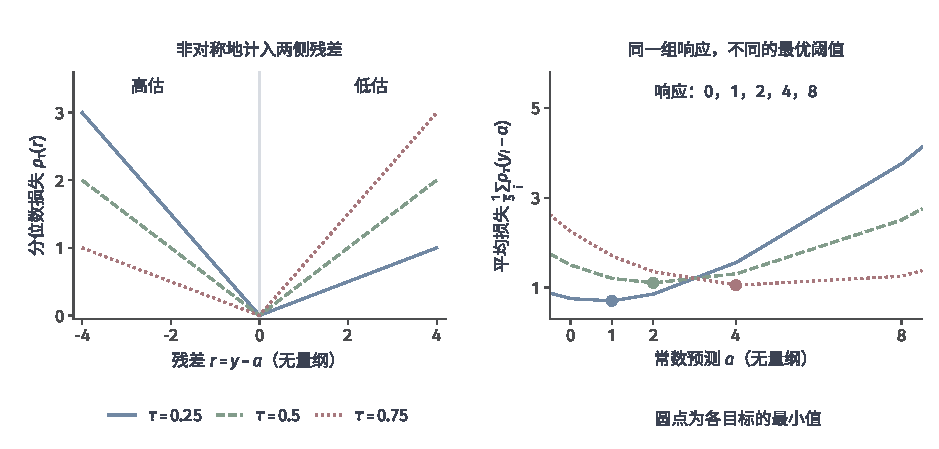
\includegraphics[width=159mm]{figures/04-classic-models/00-shared/matplotlib/regression-quantile-objective/figure.pdf}
  \caption{分位数损失怎样改变学习目标。左图中，正残差表示低估、负残差表示高估；$\tau$越大，低估一单位的代价越高。右图对固定响应$0,1,2,4,8$比较三个平均损失目标，其唯一最小点分别为$1,2,4$，对应经验分布的$0.25,0.5,0.75$分位数。数值均为无量纲教学构造，圆点表示最小值。}
  \label{fig:regression-quantile-objective}
\end{figure*}

\subsubsection{参数学习}

分位数损失在零残差处不可微，因而不宜像OLS那样直接解梯度为零的方程。我们可以把每个残差拆成正、负两部分，分别按$\tau$和$1-\tau$计分。引入非负变量$\bm u,\bm v\in\mathbb R^n$，将残差写成$\bm y-\bm X\bm w=\bm u-\bm v$，便得到线性规划
\begin{equation}
  \begin{aligned}
    \min_{\bm{w},\bm{u},\bm{v}}\quad&
      \tau\bm{1}^{\top}\bm{u}+(1-\tau)\bm{1}^{\top}\bm{v},\\
    \text{满足}\quad&
      \bm{y}-\bm{X}\bm{w}=\bm{u}-\bm{v},
      \quad\bm{u}\geq\bm{0},\ \bm{v}\geq\bm{0}.
  \end{aligned}
  \label{eq:regression-quantile-lp}
\end{equation}
若某个$u_i,v_i$同时为正，同时减小二者保持约束不变且严格降低目标，因此最优时二者不会同时为正，线性规划与原损失等价。可采用单纯形法、内点法或适合数据规模的非光滑凸优化算法；这些算法分别利用线性规划结构或直接处理非光滑凸目标。

有限样本的线性规划有可行解，目标下有界于零，因此能取得最优值，但系数和分位数都可能不唯一。停止时可比较原始与对偶可行目标的间隙，而不能直接检查普通梯度是否为零。极端分位数由较少尾部观测支持，需要特别检查验证损失与经验超越率。

\subsubsection{稀疏分位数与有序分位数}

\label{sec:regression-quantile-sparsity}

变量很多、尾部观测有限时，估计每个变量的作用容易受个别记录影响。可在平均分位数损失之外增加$\lambda\lVert\bm w\rVert_1$，使部分系数可以取零。把系数也拆成正、负两部分，仍可将这一目标写成线性规划。这与Lasso使用相同的系数约束，却保留分位数损失规定的预测对象；$\lambda$应按验证分位数损失选择，不能只凭平方误差判断。

\label{sec:regression-quantile-ordering}

若分别估计预算的中位数和较高分位数，两条曲线可能在某些输入处交叉，使较高分位数反而更低。可以同时拟合多个$\tau$，在预先指定的输入集合$\mathcal X_0$上加入顺序约束：对$\tau_1<\tau_2$，要求$\bm\phi(\bm x)^\top\bm w_{\tau_1}\leq\bm\phi(\bm x)^\top\bm w_{\tau_2}$，$\bm x\in\mathcal X_0$。对有限$\mathcal X_0$，这些是线性约束，可以和各分位数的残差分解一起求解。它们只保证指定输入处的顺序；要保证整个输入域不交叉，还需对该域施加足够的约束。联合拟合增加系数和约束数量，但避免了在各分位数之间分别选择互不协调的预测。

多个分位数能描述分布的不同位置，但有限网格不等于完整条件分布；由它们组成的预测区间仍需单独评价响应覆盖率与宽度。

\subsection{支持向量回归（SVR）}
\label{sec:regression-svr}

有些任务并不要求把每一个小偏差都继续压低，小到一定程度的误差在实际决策中与完全正确没有区别。例如，假设测量任务把$0.05$单位以内的误差都视为可接受；真实响应为$2.00$时，预测$1.98$已在容忍范围内，而预测$1.80$超出范围$0.15$。平方损失仍会区分带内的细小误差（$0.02$和$0.04$受到不同惩罚），分位数损失则对每个非零残差计分。另一种选择是让容忍范围内的损失直接为零，只对超出部分计分。\term{支持向量回归}（support vector regression, SVR）将这种损失与二次正则化结合，得到一个由训练样本加权表示的预测函数。部分样本的权重可以为零，核化以后只需保留非零权重对应的样本来计算预测。这是样本展开的稀疏性，与Lasso选择输入变量的稀疏性不同\scite{smola2004svr}。

\subsubsection{模型结构}

设$\epsilon\geq0$，定义\term{$\epsilon$不敏感损失}（$\epsilon$-insensitive loss）为$L_\epsilon(r)=(|r|-\epsilon)_+$。它把$\pm\epsilon$之间的残差视为可容忍误差，超出部分线性计入损失。线性SVR单独保留不受惩罚的截距$b$，目标为
\begin{equation}
  \min_{\bm{w},b}\;
    \frac12\lVert\bm{w}\rVert_2^2+
    C\sum_{i=1}^{n}L_\epsilon(y_i-\bm{w}^{\top}\bm{x}_i-b),
    \qquad C>0.
  \label{eq:regression-svr-objective}
\end{equation}
除以$nC$，可知它与“平均损失$+\lambda\lVert\bm{w}\rVert_2^2/2$”在$\lambda=1/(nC)$时等价。$C$越大，训练误差在目标中的相对权重越大；$\epsilon$则具有响应的单位，规定不计损失的范围。

图\ref{fig:regression-svr-objective}把损失画回响应坐标：围绕候选函数的带内偏差都不计分，带外残差只有超过边缘的部分计分。学习时还要加入斜率或核函数范数的惩罚，所以扩大容忍带、减小带外误差与选择较平缓的函数，是目标中的不同调节。

\begin{figure*}[htbp]
  \centering
  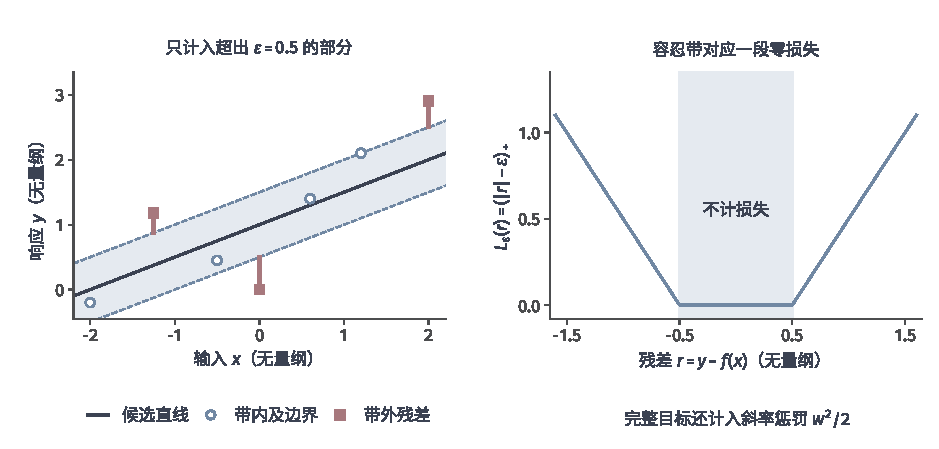
\includegraphics[width=159mm]{figures/04-classic-models/00-shared/matplotlib/regression-svr-objective/figure.pdf}
  \caption{SVR的容忍带与带外损失。左图取候选$f(x)=1+x/2$、$\epsilon=0.5$，圆点位于带内或边界，方点位于带外；红色竖段只标记超出带边缘的部分。右图将同一规则写成残差损失，带内损失为零、带外线性增长。构造样本的损失之和为$1.2$，斜率惩罚为$0.125$，因此该候选的完整目标为$0.125+1.2C$；图中不假定它是最优解。}
  \label{fig:regression-svr-objective}
\end{figure*}

损失在容忍带边缘不可微，直接用普通梯度求解并不方便。我们可以用两个非负量$\xi_i^+,\xi_i^-\geq0$，分别记录残差从两侧超出容忍带的部分；损失于是成为它们的和，而预测条件变成线性约束。这个等价形式也便于推导只依赖样本内积的对偶问题：
\begin{equation}
  \begin{aligned}
    \min_{\bm{w},b,\bm{\xi}^+,\bm{\xi}^-}\quad&
       \tfrac12\lVert\bm{w}\rVert_2^2+C\sum_i(\xi_i^++\xi_i^-),\\
    \text{满足}\quad&
       y_i-\bm{w}^{\top}\bm{x}_i-b\leq\epsilon+\xi_i^+,\\
      &\bm{w}^{\top}\bm{x}_i+b-y_i\leq\epsilon+\xi_i^-,\\
      &\xi_i^+,\xi_i^-\geq0,\qquad i=1,\ldots,n.
  \end{aligned}
  \label{eq:regression-svr-primal}
\end{equation}
固定预测时，由$C>0$可知最优松弛量恰为超出带宽的部分。$\epsilon=0$对应带二次惩罚的绝对损失回归。对固定有限数据，若$\epsilon\geq(\max_i y_i-\min_i y_i)/2$，则$\bm{w}=\bm{0}$和某个常数$b$已能使全部样本进入容忍带，目标取得零值。截距在此时可能不唯一。

\subsubsection{参数学习}

原问题是在可行参数中寻找最小目标值，为什么下面会出现一个最大化问题？把各不等式写成“左边不大于零”，分别乘以非负的拉格朗日乘子并加到目标中，就得到拉格朗日函数。在任一可行点，这些附加项都不大于零；固定乘子，再对全部原始变量取下确界，便得到原问题最优值的一个下界。选择乘子把这个下界尽量抬高，就是\term{对偶}（dual）最大化。乘子在这里用于构造下界；若最佳下界等于原问题的最小值，就称为\term{强对偶}（strong duality）。

下面用凸优化条件判断这一对应何时成立。为方便首次接触这些名词的读者，先用一句话说明它们各自扮演的角色：拉格朗日乘子可以理解为每条约束“被违反的价格”，违反越严重、价格越高，于是原问题转化为在这些价格下的权衡；Slater条件是一个保证“抬高下界”这条路能够恰好达到原问题最优值的正则性条件，它在当前凸问题中用于建立强对偶；KKT条件则是最优解必须同时满足的一份清单，把原始可行性、对偶可行性、驻点条件和互补松弛放在同一组方程中，其中互补松弛要求“约束没有被绷紧时，它的价格必须为零”，即乘子与对应约束余量的乘积为零。在凸问题满足Slater条件时，满足这份清单对最优性既必要又充分；分类SVM中的对应条件见式\eqref{eq:classification-svm-hard-kkt}。

为前两组约束引入乘子$\alpha_i^+,\alpha_i^-\geq0$，为松弛量非负约束引入$\mu_i^+,\mu_i^-\geq0$。令$r_i=y_i-\bm{w}^{\top}\bm{x}_i-b$，拉格朗日函数为
\[
  \begin{aligned}
    \mathcal{L}={}&\tfrac12\lVert\bm{w}\rVert_2^2
       +C\sum_i(\xi_i^++\xi_i^-)
       +\sum_i\alpha_i^+(r_i-\epsilon-\xi_i^+)\\
       &+\sum_i\alpha_i^-(-r_i-\epsilon-\xi_i^-)
       -\sum_i(\mu_i^+\xi_i^++\mu_i^-\xi_i^-).
  \end{aligned}
\]
分别对$\bm{w},b,\xi_i^\pm$求导，得到
\[
  \bm{w}=\sum_i(\alpha_i^+-\alpha_i^-)\bm{x}_i,\qquad
  \sum_i(\alpha_i^+-\alpha_i^-)=0,\qquad
  C-\alpha_i^\pm-\mu_i^\pm=0.
\]
最后一式给出$0\leq\alpha_i^\pm\leq C$。记$\beta_i=\alpha_i^+-\alpha_i^-$，消去原始变量后，对偶问题为
\begin{equation}
  \begin{aligned}
    \max_{\bm{\alpha}^+,\bm{\alpha}^-}\quad&
       -\tfrac12\sum_{i,j}\beta_i\beta_j\bm{x}_i^{\top}\bm{x}_j
       -\epsilon\sum_i(\alpha_i^++\alpha_i^-)
       +\sum_i y_i\beta_i,\\
    \text{满足}\quad&
       \sum_i\beta_i=0,\qquad 0\leq\alpha_i^\pm\leq C.
  \end{aligned}
  \label{eq:regression-svr-dual}
\end{equation}
原始问题凸，选择足够大的正松弛量即可严格满足不等式，因此满足Slater条件，强对偶成立。对偶是带盒约束与一个线性等式约束的凸二次规划的最大化写法，可通过分解算法逐步更新少量变量；每次更新应保持等式约束，并以最优性残差作为停止依据。

得到乘子后，若$0<\alpha_i^+<C$，互补松弛给出$r_i=\epsilon$，所以$b=y_i-\bm{w}^{\top}\bm{x}_i-\epsilon$；若$0<\alpha_i^-<C$，则$b=y_i-\bm{w}^{\top}\bm{x}_i+\epsilon$。可对多个此类样本的截距估计取平均以减小数值误差。若没有内点乘子，应根据全部KKT不等式求可行截距区间，不能假设总能找到一个严格介于$0$与$C$之间的乘子。

\subsubsection{核SVR与支持样本}
\label{sec:regression-svr-theory}
\label{sec:regression-rkhs-foundations}
\label{sec:regression-kernel-svr}

原始特征不足以表达弯曲关系时，可以保留同一个容忍带损失，只把对偶中的内积换成合法核$K(\bm x_i,\bm x_j)$。这等于在核所表示的特征空间中惩罚权重长度，预测变为
\begin{equation}
 f(\bm x)=\sum_{i=1}^n\beta_iK(\bm x_i,\bm x)+b.
 \label{eq:regression-kernel-svr-prediction}
\end{equation}
核的合法性与常用形式见第\ref{sec:classic-overview-kernel-validity}节和第\ref{sec:classic-overview-common-kernels}节。训练仍解式\eqref{eq:regression-svr-dual}的盒约束二次规划，只需更换Gram矩阵；核、$C$与$\epsilon$则一起由训练内验证选择。

为说明这里惩罚的对象，把$K(\bm x_i,\cdot)$看成关于新输入的函数，称为核截面（kernel section）。若$h=\sum_i a_iK(\bm x_i,\cdot)$、$v=\sum_j c_jK(\bm z_j,\cdot)$，核定义的内积和范数满足
\begin{equation}
 \begin{aligned}
 \langle h,v\rangle_{\mathcal H_K}
 &=\sum_{i,j}a_ic_jK(\bm x_i,\bm z_j),\\
 \|h\|_{\mathcal H_K}^2&=\bm a^\top\bm K\bm a.
 \end{aligned}
 \label{eq:regression-rkhs-inner-product}
\end{equation}
相差零范数的表示视为同一函数，并纳入范数极限后，就得到\term{再生核Hilbert空间}（reproducing kernel Hilbert space, RKHS），记为$\mathcal H_K$。它把特征空间中的长度写成可以由核值计算的函数范数，而不是展开系数的普通欧氏长度。再生关系
\begin{equation}
 h(\bm x)=\langle h,K(\bm x,\cdot)\rangle_{\mathcal H_K}
 \label{eq:regression-rkhs-reproducing}
\end{equation}
表示通过与一个核截面取内积即可恢复点值。核SVR的范数惩罚作用于$h$，不作用于单独的截距$b$；同一核空间也可配平方损失得到核岭回归，不能仅凭使用同一个核就视为同一个学习目标\scite{rasmussen2006}。

预测时只需保留$\beta_i\ne0$的训练样本。KKT条件说明它们来自容忍带外或边界，但不能反过来说每个边界样本都有非零系数。
\begin{lemma}[SVR的样本系数与残差]
 \label{thm:regression-svr-support}
 当$\epsilon>0$时，严格带内$|r_i|<\epsilon$有$\alpha_i^+=\alpha_i^-=0$；正向带外$r_i>\epsilon$有$\alpha_i^+=C,\alpha_i^-=0$，负向带外则相反。边界处相应乘子可取$[0,C]$中的值，包括零。因此$\beta_i\ne0$蕴含$|r_i|\geq\epsilon$，边界上的反向蕴含不成立。
\end{lemma}
最优松弛量为$(r_i-\epsilon)_+$和$(-r_i-\epsilon)_+$。严格松弛的约束由互补松弛迫使乘子为零，正松弛量则由$C-\alpha_i^\pm-\mu_i^\pm=0$迫使对应乘子为$C$，这就给出上述区别。$\epsilon=0$时两个边界重合，不能照搬两侧分开的结论。

完整存储核矩阵需要$O(n^2)$空间；缓存与分解求解能改变实际成本。预测约需$n_{\mathrm{SV}}$次核计算，线性核则可以预先合并为$\bm w$，使预测恢复为$O(d)$。支持样本少减少的是预测访问量，并不直接保证未来误差小。基本SVR优化的是容忍带外的损失，其总体最优中心一般不同于条件均值；若要条件分位数或响应分布，应使用相应损失或似然。

\subsection{广义线性模型（GLM）}
\label{sec:regression-glm}

预测每天的交易次数时，均值必须非负；预测交易是否成功时，均值是$[0,1]$中的概率。原始特征上的线性函数不保证这些范围。例如构造拟合$10-2x$在$x=0,1$时都为正，却在$x=6$时给出负次数。仅给平方损失增加惩罚并不能自动排除这种预测；平方损失也没有为这些响应规定均值与方差的关系。\term{广义线性模型}（generalized linear model, GLM）把响应分布、均值和线性预测器连接起来。Nelder与Wedderburn在1972年给出这一统一框架，使高斯、二项和Poisson等响应可以沿同一条似然与加权最小二乘路线处理；扩展的关键是响应分布与链接，而不只是增加多项式特征\scite{nelder1972glm}。

\subsubsection{模型结构}

高斯（连续对称）、伯努利（0/1）、Poisson（计数）看起来是三类毫不相干的响应，但它们的拟合过程可以共用同一套公式，关键是把它们写成一个共同的形式。这不仅是形式上的整齐：一旦写成统一形式，均值与方差的关系、最大似然的迭代更新都能由同一组量推出，只需为每种响应填入不同的函数，而不必为每类响应各推一遍算法。条件于输入，假设响应相互独立，密度或概率质量函数具有指数族形式
\begin{equation}
  p(y_i\mid\theta_i,\varphi)
  =\exp\!\left\{
    \frac{y_i\theta_i-b(\theta_i)}{a(\varphi)}
    +c(y_i,\varphi)\right\},\qquad a(\varphi)>0.
  \label{eq:regression-exponential-family}
\end{equation}
$\theta_i$是自然参数，$\varphi$是离散度参数或尺度参数；此处为便于推导，所有观测使用相同的$a(\varphi)$。函数$a,b,c$的形式由选定的分布族确定，并不作为三个未知函数一起学习。例如，均值为$\mu_i>0$的Poisson分布可写成
\[
  p(y_i\mid\mu_i)
  =\frac{\mu_i^{y_i}e^{-\mu_i}}{y_i!}
  =\exp\{y_i\log\mu_i-\mu_i-\log(y_i!)\}.
\]
逐项对照式\eqref{eq:regression-exponential-family}，可得$\theta_i=\log\mu_i$、$b(\theta_i)=e^{\theta_i}$、$a(\varphi)=1$、$c(y_i,\varphi)=-\log(y_i!)$。这里没有额外待估的离散度参数，自然参数也不是均值本身。

一般情形下，假定支持集不随$\theta_i$改变，并允许交换积分（离散情形为求和）与微分。密度积分为$1$，对$\theta_i$求导得到$\mathbb{E}[Y_i-b'(\theta_i)]=0$；再求一次导数得到
\[
  \mathbb{E}\!\left[
    \frac{(Y_i-b'(\theta_i))^2}{a(\varphi)^2}
      -\frac{b''(\theta_i)}{a(\varphi)}\right]=0.
\]
因此均值与方差为
\begin{equation}
  \mu_i=b'(\theta_i),\qquad
  \operatorname{Var}(Y_i\mid\bm{x}_i)
  =a(\varphi)b''(\theta_i)=a(\varphi)V(\mu_i).
  \label{eq:regression-glm-moments}
\end{equation}
函数$V$描述方差怎样随均值变化。GLM再引入线性预测器$\eta_i=\bm{\phi}(\bm{x}_i)^{\top}\bm{w}$与\term{链接函数}（link function）$g$，令$g(\mu_i)=\eta_i$。链接作用于条件均值，而不是把每个观测$y_i$变换后做OLS。若$\eta_i=\theta_i$，称为规范链接。

表\ref{tab:regression-glm}列出三种基本组合。伯努利模型的均值就是成功概率，因此logistic回归既可作为概率回归理解，也可在给定决策阈值后用于分类。第\ref{sec:classification-logistic}节沿用伯努利似然、logit链接与IRLS计算，但把重点转向类别标签的概率、决策阈值与校准；本节则借这一特例说明GLM中响应分布、链接和均值方差关系的共同结构。Poisson模型采用对数链接，使$\mu_i=\exp(\eta_i)>0$；响应是整数，条件均值却不必为整数。

\begin{table}[htbp]
  \centering
  \begin{tabular}{llll}
    \toprule
    响应模型 & $b(\theta)$ & 规范链接$g(\mu)$ & $V(\mu)$\\
    \midrule
    高斯 & $\theta^2/2$ & $\mu$ & $1$\\
    伯努利 & $\log(1+e^\theta)$ & $\log\frac{\mu}{1-\mu}$ & $\mu(1-\mu)$\\
    Poisson & $e^\theta$ & $\log\mu$ & $\mu$\\
    \bottomrule
  \end{tabular}
  \caption{GLM的三个常用特例。高斯模型的$a(\varphi)=\sigma^2$，后两者的$a(\varphi)=1$。链接保证均值范围，分布假设进一步规定条件方差。}
  \label{tab:regression-glm}
\end{table}

二项分布可处理已知试验次数下的成功数；Gamma模型可处理正连续响应。链接选择并不唯一，必须同时满足自然参数域和均值域的要求。Poisson的均值方差相等也可能与数据不符。例如，在固定输入后，若响应方差大于其均值，就出现了相对于Poisson模型的过度离散（overdispersion）；若生成机制带来的零响应概率超过所拟合计数模型给出的概率，则需要考虑零膨胀（zero inflation）。这些差异以及观测相关性需要额外建模，不能靠对数链接本身解决。

\subsubsection{参数学习}

一般GLM的均值随系数非线性变化，不能像OLS那样一次解线性方程得到最大似然解。一个自然的策略是反复“在当前猜测附近把问题局部拉直，解一个熟悉的加权最小二乘，再用结果更新猜测”，直到收敛，这就是下面的IRLS。要选择增大对数似然的方向，我们先计算它对系数的导数，这个梯度称为得分。记$\bm z_i=\bm\phi(\bm x_i)$，设计矩阵第$i$行为$\bm z_i^\top$，暂将$\varphi$视为已知。由$d\mu_i/d\theta_i=V(\mu_i)$及$d\eta_i/d\mu_i=g'(\mu_i)$，利用链式法则得到
\begin{equation}
  \bm{U}(\bm{w})
  =\sum_i\frac{y_i-\mu_i}
    {a(\varphi)V(\mu_i)g'(\mu_i)}\bm{z}_i.
  \label{eq:regression-glm-score}
\end{equation}
在所需导数存在且$g'(\mu_i)\ne0$时，期望负Hessian即Fisher信息$\bm{X}^{\top}\bm{W}\bm{X}$，其中
\[
  W_{i,i}=\frac{1}{a(\varphi)V(\mu_i)[g'(\mu_i)]^2}.
\]
\term{Fisher评分}（Fisher scoring）用这个期望曲率修正当前参数，更新$\bm{w}^{+}=\bm{w}+(\bm{X}^{\top}\bm{W}\bm{X})^{-1}\bm{U}(\bm{w})$。要把它写成加权最小二乘，需要先把响应尺度上的误差换算成线性预测器尺度上的修正。在当前均值附近，链接函数的一阶近似为$g(\mu_i+\Delta\mu)\approx\eta_i+g'(\mu_i)\Delta\mu$；将残差$y_i-\mu_i$作为局部修正信号，便得到\term{工作响应}（working response）
\[
  z_i^{\mathrm{work}}
    =\eta_i+(y_i-\mu_i)g'(\mu_i),
\]
它是本轮局部子问题的目标值，会随当前参数改变，并非把真实标签永久变成$g(y_i)$。固定当前参数时，这个仿射换算后的响应方差为$a(\varphi)V(\mu_i)[g'(\mu_i)]^2$，其倒数正是$W_{i,i}$；换算后方差较大的观测因而权重较小。代入可得$\bm{U}=\bm{X}^{\top}\bm{W}(\bm{z}^{\mathrm{work}}-\bm{X}\bm{w})$，从而
\begin{equation}
  \bm{w}^{+}
  =(\bm{X}^{\top}\bm{W}\bm{X})^{-1}
     \bm{X}^{\top}\bm{W}\bm{z}^{\mathrm{work}}.
  \label{eq:regression-irls}
\end{equation}
这就是\term{迭代重加权最小二乘}（iteratively reweighted least squares, IRLS）：在当前均值附近构造一个加权平方子问题。实际使用分解求解线性方程，检查秩、合法参数域以及对数似然是否上升。若完整步使对数似然下降，则采用阻尼或线搜索缩小这一步。各观测共享的$a(\varphi)$在无惩罚参数更新中可以约去，但在信息矩阵和方差计算中不能遗漏。

规范链接下，$\theta_i=\eta_i$，负对数似然的Hessian为
\[
  \frac{1}{a(\varphi)}
  \bm{X}^{\top}\operatorname{diag}(b''(\eta_i))\bm{X}.
\]
它半正定，因此目标凸；若$b''(\eta_i)>0$且设计列满秩，则有限参数域内严格凸。这时Newton法与Fisher评分具有相同的曲率矩阵，但完整步长不自动保证每次都提高似然，更不能保证有限最优解存在。

\subsubsection{链接、特征与有限解}
\label{sec:regression-glm-theory}

响应分布和均值结构需要分别检查。Poisson对数链接配特征$1,x$只能给出$\mu(x)=\exp(b+wx)$；若真实对数均值含$x^2$，应加入相应特征。若均值正确但响应方差明显大于均值，则是Poisson分布的限制，单独增加均值特征不能解除它。下一小节用平滑项改变变量作用，第\ref{sec:regression-distributional}节则进一步让尺度等分布参数随输入变化。

凸性也不保证有限最大似然解。以伯努利模型为例，若存在一个方向将所有正、负样本严格分开，沿此方向放大系数可使负对数似然不断趋近零，却没有有限系数取到零。参数约束或正则化可以限制这种增长，但若截距不惩罚，仍应检查截距方向。Poisson的曲率$e^\eta$没有全空间上界，因此迭代中应检查合法参数范围与似然改进，不能把OLS的固定步长直接套来。

验证时还要按所交付的分布评分，而不是只检查均值平方误差。拟合相同均值的两个响应模型，仍可能给极端观测分配完全不同的概率；均值、离散程度和尾部诊断分别约束模型的不同部分。

\subsection{广义可加模型（GAM）}
\label{sec:regression-gam}

若上一节的GLM只使用原始特征，线性预测器就是$\eta=b+\sum_j w_jx_j$。固定其他属性，楼龄每增加一年，链接尺度上的预测总改变同一个$w_{\mathrm{age}}$。如果采用恒等链接，这就是每年固定增减同样价格；采用对数链接，则是每年固定乘上同一个比例。

考虑一个教学构造：其余房屋属性固定，年龄$t\geq0$以年计，价格以万元计，条件均值为$m(t)=200+100e^{-t/10}$。它在第0、10、20年约为300、236.8、213.5万元。第一个十年下降约63.2万元，第二个十年只下降约23.3万元；一条直线若配合前一段的下降速度，就会把后一段的降幅预测得过大。换成对数链接也不能完整解决：$d\log m(t)/dt=-10e^{-t/10}/(200+100e^{-t/10})$随楼龄变化，仍不是一个常数。这里缺少的是单个变量在不同取值处可以具有不同作用，而不只是输出取值范围。

可以为楼龄预先设计平方项、指数项或样条基，但我们还希望从数据估计曲线，同时单独检查面积与楼龄各自怎样影响预测。\term{广义可加模型}（generalized additive model, GAM）让每个特征贡献一个一维函数，再把这些贡献相加。Hastie与Tibshirani在1986年系统阐述了这一扩展：保留GLM的分布与链接，用平滑函数替代单特征的线性项。在刚才的恒等链接例子中，楼龄项可以取$f_{\mathrm{age}}(t)=100e^{-t/10}$再按约定移除常数，截距吸收基准价格；其导数随$t$变化，因而不再强求两个十年使用同一降幅。面积等属性也可分别使用自己的函数。它保留逐特征检查作用形状的便利，并通过可加结构限制需要学习的交互关系\scite{hastie1986gam}。

\subsubsection{模型结构}

沿用GLM的响应分布与链接，GAM写成
\begin{equation}
  g(\mu_i)=b+\sum_{j=1}^{d}f_j(x_{i,j}),
  \qquad \sum_{i=1}^{n}f_j(x_{i,j})=0.
  \label{eq:regression-gam}
\end{equation}
中心化约束把常数部分留给截距$b$，使各$f_j$描述相对于样本平均水平的变化。它消除了常数在各项之间任意移动的歧义，却不能解决所有不可识别问题：若两个输入完全相同，两个光滑项仍可能互相抵消，需要进一步约束或合并表示。

恒等链接下，$f_j$直接作用于条件均值；非线性链接下，它作用于链接尺度。例如可加logistic模型中的函数描述对数几率的变化，不能直接当作概率变化。没有显式交互项时，GAM不能表达任意多维关系。每项可画图并不意味着它具有因果含义，相关特征仍会影响解释。

\subsubsection{参数学习}

用预定样条基展开$f_j(x)=\sum_{k=1}^{K_j}\gamma_{j,k}B_{j,k}(x)$后，GAM仍可写成扩大设计矩阵上的GLM。为限制每条曲线的起伏，我们再惩罚其斜率的变化：二阶导数越大，斜率改变得越急。为第$j$个变量预先选定有限建模区间$I_j=[l_j,u_j]$，并假定各基函数的二阶导数在$I_j$上平方可积。曲率惩罚$\int_{I_j}[f_j''(x)]^2\,dx$可写成$\bm{\gamma}_j^{\top}\bm{S}_j\bm{\gamma}_j$，其中
\[
  (\bm{S}_j)_{k,l}=\int_{I_j}B_{j,k}''(x)B_{j,l}''(x)\,dx.
\]
任意$\bm{a}$满足$\bm{a}^{\top}\bm{S}_j\bm{a}=\int_{I_j}(\sum_k a_kB_{j,k}''(x))^2dx\geq0$，故惩罚矩阵半正定。积分区间决定在哪些取值处计算曲率，也参与确定矩阵$\bm S_j$。常数和一次函数的二阶导数为零，属于该惩罚的零空间，因此$\lambda_j$很大时通常留下线性成分，而不是自动把整项置零。

在满足中心化约束的坐标中，把截距和全部基系数组成$\bm{\gamma}$，设计矩阵记为$\bm{B}$。固定响应分布中的尺度等其他参数后，记整批训练记录的总对数似然为$\ell_{\mathrm{tot}}(\bm\gamma)=\sum_{i=1}^n\log p(y_i\mid\bm x_i;\bm\gamma)$。它与前文的单条记录损失$\ell(y,a)$含义不同：这里对全部记录的对数概率或对数密度求和，并希望它尽量大；取负号后才能与曲率惩罚一起最小化。

将各项惩罚合并成块矩阵$\bm S_\lambda$，使$\bm\gamma^\top\bm S_\lambda\bm\gamma=\sum_j\lambda_j\bm\gamma_j^\top\bm S_j\bm\gamma_j$，截距与其他未惩罚方向不增加惩罚。设计矩阵和惩罚矩阵都使用同一组消去中心化约束后的坐标。这样，系数学习同时比较总对数似然与各条曲线的起伏，可最小化
\[
  -\ell_{\mathrm{tot}}(\bm{\gamma})+\tfrac12\bm{\gamma}^{\top}
       \bm{S}_{\lambda}\bm{\gamma}.
\]
固定平滑参数$\lambda_j$时，沿用GLM中当前工作响应$\bm z^{\mathrm{work}}$与权重$\bm W$，把负对数似然局部换成加权平方子问题。加上同一个二次惩罚后，对系数求导并令导数为零，便得到惩罚IRLS每一步求解的线性方程：
\begin{equation}
  (\bm{B}^{\top}\bm{W}\bm{B}+\bm{S}_{\lambda})
       \bm{\gamma}^{+}
  =\bm{B}^{\top}\bm{W}\bm{z}^{\mathrm{work}}.
  \label{eq:regression-gam-irls}
\end{equation}
只有数据曲率与惩罚共同排除全部未约束零方向时，系数解才唯一。设展开后总维数为$q$，稠密加权平方子问题约需$O(nq^2+q^3)$运算；稀疏局部基可以改变这个代价。预测则需计算相应基函数，不能始终按原始维数$d$计为$O(d)$。

高斯恒等链接下也可采用\term{回代拟合}（backfitting）：固定其他函数，以部分残差$y_i-b-\sum_{k\ne j}f_k(x_{i,k})$拟合第$j$项，再中心化并循环。对固定有限基、正定惩罚平方系统，精确块更新等价于块Gauss--Seidel迭代，收敛到唯一解；若任意组合不对应共同目标的平滑器，则需另行证明。非高斯响应可把这种循环嵌入工作响应更新。

平滑参数决定拟合曲线的曲折程度。仅凭训练残差下降，不能判断未见响应上的误差是否减少，因此选择平滑参数时需要估计样本外误差。交叉验证直接使用未参与当前拟合的响应。高斯恒等链接下，固定平滑参数的拟合还可写成$\widehat{\bm y}=\bm H_\lambda\bm y$；矩阵$\bm H_\lambda$将响应映射为拟合值，其第$i$个对角元表示$y_i$增加一单位时，拟合值$\widehat y_i$改变多少。对角元之和$\operatorname{tr}(\bm H_\lambda)$称为有效自由度，衡量这些响应对各自拟合值的总影响。

为了看清为什么要用这些对角元修正残差，可以先逐条留出记录再预测。\term{留一法}（leave-one-out cross-validation, LOOCV）在每一轮删去一条记录，用其余记录拟合，再评价被删记录的预测误差。这里固定原来的基函数、约束与惩罚矩阵，并要求完整数据与删去任一记录后的惩罚平方问题都有唯一解。记$h_i=(\bm H_\lambda)_{i,i}<1$，$\widehat m_i^{(-i)}$表示不使用第$i$条响应时，在$\bm x_i$处得到的预测值。

我们可以用一次完整拟合来恢复这些留一预测。设想把完整响应向量的第$i$项改成$\widehat m_i^{(-i)}$，其他项不变。在删去第$i$条记录后得到的解处，新补入的这一项残差恰为零，对平方目标的梯度也为零，因此它仍解同一个固定惩罚下的完整问题。另一方面，线性映射$\bm H_\lambda$表明，第$i$项响应的这次改动使第$i$个拟合值改变$h_i(\widehat m_i^{(-i)}-y_i)$。两种描述对应同一解，故
\begin{equation}
 \begin{aligned}
 \widehat m_i^{(-i)}
   &=\widehat y_i+h_i(\widehat m_i^{(-i)}-y_i),\\
 y_i-\widehat m_i^{(-i)}
   &=\frac{y_i-\widehat y_i}{1-h_i},\\
 \operatorname{CV}_{\mathrm{LOO}}(\lambda)
   &=\frac1n\sum_{i=1}^n
       \left(\frac{y_i-\widehat y_i}{1-h_i}\right)^2.
 \end{aligned}
 \label{eq:regression-gam-loocv}
\end{equation}
因此，分母$1-h_i$将训练残差换算成去除该条响应自我影响后的残差；$h_i$越接近1，直接使用训练残差就越可能低估删去该响应后的误差。以上等式依赖固定的二次目标及相同的惩罚，并不是对任意数据依赖的平滑程序都成立。

逐条修正需要保留每个$h_i$。广义交叉验证（generalized cross-validation, GCV）进一步用平均对角元$\bar h=\operatorname{tr}(\bm H_\lambda)/n$替代它们，以平均敏感程度近似留一修正。将这个共同分母提出平方残差之和，就得到
\begin{equation}
 \operatorname{GCV}(\lambda)
 =\frac{\lVert\bm y-\widehat{\bm y}\rVert_2^2/n}
        {[1-\operatorname{tr}(\bm H_\lambda)/n]^2},
 \qquad \operatorname{tr}(\bm H_\lambda)<n.
 \label{eq:regression-gam-gcv}
\end{equation}
当有效自由度接近样本数时，修正因子变大；训练残差的下降需要足以抵偿这项复杂度代价，才会降低GCV。若不同记录的$h_i$差异很大，用平均值替代各个对角元就可能与真正的留一误差相差较大。这是固定线性平滑器下的准则，不能用基函数个数直接代替有效自由度，也不能把某次GCV下降直接当作未来误差下降的证明。

平滑参数还可通过概率模型估计。高斯恒等链接下，将半正定惩罚的零空间保留为未惩罚项，把其余方向重新缩放，模型可以写成
\begin{equation}
 \begin{gathered}
 \bm y=\bm X_0\bm\beta+\bm Z_u\bm u+\bm\varepsilon,\\
 \bm u\sim N(\bm0,\tau^2\bm I),\qquad
 \bm\varepsilon\sim N(\bm0,\sigma^2\bm I).
 \end{gathered}
 \label{eq:regression-gam-random-effects}
\end{equation}
其中$\bm u$与噪声独立，$\bm X_0\bm\beta$含截距及其他未惩罚方向。固定方差时，负对数先验与似然给出残差平方和及$\lambda\|\bm u\|_2^2$惩罚，$\lambda=\sigma^2/\tau^2$。允许曲线系数有较大方差，就对应较弱平滑；这类系数称为随机效应（random effect）。

选择方差时，应先按高斯分布积分掉$\bm u$，得到边缘协方差$\tau^2\bm Z_u\bm Z_u^\top+\sigma^2\bm I$，再估计两个方差，而不能只把最优系数代回残差项。受限最大似然（restricted maximum likelihood, REML）使用与$\bm X_0$各列正交的响应组合估计方差，使已经用于估计均值的方向不再当作新的噪声信息。多个平滑项可对应不同方差；非高斯响应则需要相应近似。外层平滑参数的选择与固定参数下的IRLS是不同优化问题，不能继承同一求解保证\scite{wood2011reml}。

\subsubsection{交互项与分布参数的扩展}

\label{sec:regression-gam-interactions}

若楼龄对价格的作用还取决于房屋面积，只把楼龄曲线与面积曲线相加便不够。可以在链接尺度上加入少数二变量函数$f_{j,k}(x_j,x_k)$，让一个变量的作用随另一个变量改变。例如$x_1x_2$使$x_1$的作用随$x_2$改变，加入这一交互项就能表示；继续增加单变量基函数则不能达到这个目的。

交互项需与主效应作区分，否则同一段单变量变化既可归入$f_j$，也可藏在$f_{j,k}$中。实际展开要约束或去除与主效应基空间重叠的部分，再对剩余交互成分施加平滑惩罚。二变量基通常包含更多系数，需要更多联合输入覆盖，也使逐特征解释变成对两变量响应面的检查，因此应围绕明确的交互问题增加这些项。

一种具体展开是$f_{j,k}(x_j,x_k)=\sum_{r,s}\theta_{r,s}B_{j,r}(x_j)B_{k,s}(x_k)$，用两个变量的基函数乘积作新设计列。去除与主效应重叠的列后，把$\theta_{r,s}$与原单变量系数一起学习，目标仍是负对数似然加各块平滑惩罚，求解仍用扩展设计的惩罚IRLS。新输入先计算这些单变量与乘积基，再通过同一链接反变换得到均值；增加交互改变的是预测结构，不是只给原曲线换一个平滑参数。

\paragraph{让尺度也随输入变化}

\label{sec:regression-distributional}

条件均值相同，并不意味着响应的波动范围相同。考虑两个教学区域的价格都以$100$为条件均值，标准差却分别为$10$与$40$；只改变均值的高斯GLM或GAM，仍会给两者使用同一个噪声尺度。

\term{分布回归}（distributional regression）提供了完整条件分布的另一条入口：先选择响应分布族，再让位置、尺度或形状等多个分布参数分别依赖输入。广义可加位置、尺度与形状模型（generalized additive models for location, scale and shape, GAMLSS）允许用线性项或平滑项建模这些参数，因而能表达均值不变但条件方差、偏度或尾部随输入变化的情形\scite{rigby2005gamlss}。它描述整个响应分布，与只拟合若干分位点的目标不同。代价是必须选择分布族、链接与各参数的结构，并用样本外的分布评分和校准诊断检查预测。

以高斯位置—尺度模型为例，位置就是均值，尺度就是标准差。分别令
\[
 \begin{aligned}
 \mu_i&=b_\mu+\sum_j f_{\mu,j}(x_{i,j}),\\
 \log\sigma_i&=b_\sigma+\sum_j f_{\sigma,j}(x_{i,j}).
 \end{aligned}
\]
并设$Y_i\mid\bm x_i\sim N(\mu_i,\sigma_i^2)$。两个区域可以共享均值$100$，却通过第二套函数分别给出标准差$10$与$40$。这不是给均值多加一个基函数，而是增加了一套决定响应波动的预测器；其他响应族的位置参数未必就是均值，应按该族的参数定义解释。

用预定基展开两套函数后，待估量是两组系数。略去常数，训练目标为
\[
 \sum_i\left\{\log\sigma_i+
              \frac{(y_i-\mu_i)^2}{2\sigma_i^2}\right\}
       +\frac12\operatorname{pen}(\bm\gamma_\mu,\bm\gamma_\sigma),
\]
其中$\operatorname{pen}$是各平滑项的加权二次惩罚。固定尺度时，均值系数学习是权重$1/\sigma_i^2$的惩罚最小二乘；固定均值时，则按残差与$\log\sigma_i$求导更新尺度系数。算法可交替更新参数块，或用联合Newton/Fisher评分，检查似然改进并选择平滑强度。对过于灵活的尺度函数，还需防止围绕少量记录把方差压得过小；联合目标不再因各块形式简单而自动全局凸。预测时输出由两套函数共同确定的分布，再用分布评分与校准检查，而不只比较均值MSE。

是否增加交互项，取决于遗漏的是否是变量之间的共同作用；是否扩大响应族或建模尺度，则取决于遗漏的是否是条件分布形状。两者改变不同部分，都应连同平滑强度在训练内选择。

\subsection{预测目标与模型关系}
\label{sec:regression-linear-summary}

本节各方法的共同点是可利用线性预测器或线性基展开，差异则落在预测对象和约束方式上。表\ref{tab:regression-linear-comparison}保留这些最直接影响选择的区别。平方损失、分位数损失和$\epsilon$不敏感损失本身都不要求响应高斯；只有明确采用概率模型时，分布假设才成为似然和推断的依据。

\begin{table*}[htbp]
  \centering
  \begin{tabularx}{\linewidth}{@{}l>{\RaggedRight\arraybackslash}X>{\RaggedRight\arraybackslash}X>{\RaggedRight\arraybackslash}X@{}}
    \toprule
    方法 & 拟合目标 & 主要结构或约束 & 需要单独检查的边界\\
    \midrule
    OLS & 平方损失下的条件均值 & 固定线性特征展开 & 秩、共线性、模型失配\\
    正则化线性回归 & 拟合与惩罚的折中 & 稠密收缩、坐标或组稀疏 & 尺度、调参、选择稳定性\\
    分位数回归 & 指定条件分位数 & 非对称线性残差损失 & 尾部信息、交叉、杠杆点\\
    SVR & 容忍带外的残差损失 & 二次范数与可选核展开 & 核选择、样本展开规模\\
    GLM & 指定分布的似然 & 均值链接与线性预测器 & 分布、解的存在与设计\\
    GAM & 惩罚似然或平方损失 & 可加函数与平滑约束 & 交互遗漏、可识别性\\
    \bottomrule
  \end{tabularx}
  \caption{线性回归及其扩展的比较。表中列出本节采用的基本形式；分位数回归和GLM也可加正则，概率区间的构造还需额外假设或校准。}
  \label{tab:regression-linear-comparison}
\end{table*}

相关特征使系数难以分辨时，岭与弹性网收缩原坐标中的系数，PCR与PLS则先压缩估计方向；前者可能压低信号，后者可能舍弃预测所需的成分。若还需要删去变量，Lasso与组Lasso分别按坐标或预定变量组选择。这些方法调整的是函数表示或系数约束，不能替代对响应目标的选择：均值、分位数与容忍带仍需各自的损失。参数稀疏选择输入特征，SVR的样本展开稀疏则减少预测时访问的训练记录，二者影响不同的成本。

若同一个变量在不同位置有不同斜率，可以增加基函数、采用核表示，或用GAM分别估计各变量的曲线。GAM通过限制交互保留逐变量解释；核表示能否覆盖所需关系取决于核所规定的候选空间，还需承担样本展开与核矩阵的成本。若缺少的是响应尺度与尾部随输入的变化，分布回归扩展的是响应分布参数，不能只靠增加均值曲线的弯曲程度解决。若关系主要由查询附近的数据支撑，就转向下一节的邻域方法。

\section{基于邻域的回归}
\label{sec:regression-instance}

沿用第\ref{sec:classic-overview-neighborhood}节定义的邻域，回归需要把附近样本的响应变成一个数值预测。$k$-NN采用局部常数平均，LOESS在邻域内拟合低阶多项式；二者的区别主要在局部模型与平滑尺度。下面分别说明响应噪声、邻域大小和查询成本怎样影响预测。

\subsection{$k$近邻回归（$k$-NN）}
\label{sec:regression-knn}

用多项式或样条回归时，我们先决定整条预测曲线由哪些基函数组成，这需要预先对关系形状作出判断。如果只愿意相信一条很弱的假设——位置相近的输入，其条件均值也应当相近——也可以暂不指定任何全局函数形式，把查询点附近的观测直接作为局部依据：预测一个点时才临时看它周围的数据，换一个查询点再重新看一次，不预先固定整条曲线。例如$m(x)=x^2$时，查询$x=1$附近的无噪声响应$m(0.9)=0.81$和$m(1.1)=1.21$，平均为$1.01$，已经接近$m(1)=1$；换到$x=0$附近，局部平均也随之改变。

$k$-NN回归为每个查询点找出$k$个最近输入，再用它们的响应平均估计条件均值。相近输入减少函数变化带来的偏差，多次观测的平均则减少响应噪声；这两个作用对邻域大小有不同要求。Stone关于非参数回归一致性的工作为这类方法提供了理论依据，具体条件与收敛对象将在下文说明\scite{stone1977regression}。

\subsubsection{模型结构}

对查询点$\bm{x}$，令$I_k(\bm{x})$为恰好包含$k$个最近样本的索引集，定义
\begin{equation}
  \widehat m_{n,k}(\bm{x})=\frac1k\sum_{i\in I_k(\bm{x})}y_i,
  \qquad 1\leq k\leq n.
  \label{eq:regression-knn}
\end{equation}
距离并列时应采用不依赖响应的固定规则或独立随机化。欧氏距离适合尺度已经可比的数值特征；若使用Mahalanobis距离，则还要估计或指定度量矩阵。特征标准化应基于训练集，类别特征的相似性也需另行定义。

$k=1$保留最近样本的响应噪声，$k=n$退化为全局平均；两者的偏差大小仍取决于真实函数，不能仅由$k$断言。

\subsubsection{参数学习}

基本$k$-NN回归不拟合固定维数的系数，但仍需保存训练样本、建立可选索引，并通过验证选择$k$和距离设定。朴素查询计算全部距离需要$O(nd)$运算，再通过选择算法找出前$k$个邻居；不必为此完整排序全部距离。

交叉验证比较候选$k$时，每个验证点只能使用相应训练折作为邻居库。用训练点预测自身会产生过于乐观的误差，尤其$k=1$时可以直接复现训练响应。若从同一响应数据学习距离或选择邻居，下面仅条件于输入的简单证明也不能原样套用。

\subsubsection{邻居数量与距离权重}
\label{sec:regression-knn-theory}

选择$k$时存在两个相反要求：邻居应近，使它们的条件均值接近查询点；邻居又应多，使响应噪声能被平均。设训练响应$Y_i=m(\bm X_i)+\varepsilon_i$，噪声条件独立、均值为零、方差不超过$\sigma^2$，邻居选择只依赖输入。固定训练输入后，预测误差分成
\[
 \widehat m_{n,k}(\bm x)-m(\bm x)
 =\frac1k\sum_{i\in I_k}[m(\bm X_i)-m(\bm x)]
  +\frac1k\sum_{i\in I_k}\varepsilon_i.
\]
第一项来自邻域内函数变化，第二项的条件方差不超过$\sigma^2/k$。若$|m(\bm x)-m(\bm z)|\leq L\|\bm x-\bm z\|_2$，将最远邻居距离记为$R_{n,k}(\bm x)$，便有
\[
 \mathbb E[(\widehat m_{n,k}(\bm x)-m(\bm x))^2\mid X_{1:n}]
 \leq L^2R_{n,k}(\bm x)^2+\frac{\sigma^2}{k}.
\]
这解释了为何不能只把$k$设得越大越好：噪声项减小的同时，邻域可能扩大。高维或无关坐标会使附近输入稀疏，需要更大区域才能获得同样多的邻居。Stone的一致性研究说明，在有限维欧氏输入、有限响应二阶矩及适当并列规则下，若随着样本量增长同时满足$k\to\infty$且$k/n\to0$，局部常数平均就能收敛到真实的条件均值\scite{stone1977regression}。这两个条件各自负责一件事：$k\to\infty$保证参与平均的观测越来越多，响应噪声能被充分抵消；$k/n\to0$保证邻居在全部样本中的占比越来越小，即使邻域半径随$k$增大，它在整个输入空间中仍收缩到查询点附近，函数变化造成的偏差因而趋于零。它描述的是样本量趋于无穷时的极限行为，并不是某个有限样本中$k$越大误差越小的保证。

\label{sec:regression-knn-weighting}

等权平均让第一个邻居与第$k$个邻居贡献相同。若邻域跨越的范围较大，可以给更近的观测较高权重，减少远处响应对查询值的影响。距离加权版本写成$\sum_i a_i(\bm x)y_i$，其中$a_i\geq0$、$\sum_i a_i=1$，权重可在邻域外置零。使用距离倒数时必须规定零距离的处理，例如仅对重合输入的响应平均，不能直接除以零。权重若集中于很少的记录，也会削弱平均噪声的作用，因此距离权重与邻居数需要共同选择。

\subsubsection{邻居检索与查询成本}

\label{sec:regression-knn-query}

保存训练记录以后，每次查询仍需找到邻居；当记录很多、查询频繁时，逐条计算距离成为主要成本。

KD树、Ball树等索引在适合的低维几何结构下可以减少搜索量，但查询复杂度依赖数据分布、查询位置与维数，最坏情况仍可能接近扫描。近似近邻以容许搜索误差换取计算节约，预测误差分析需把邻居近似的影响计入。索引和$k$的选择因此应依据当前数据的几何结构、查询预算与验证误差。



\subsection{局部加权回归（LOESS）}
\label{sec:regression-loess}

局部平均把邻域内的预测视作常数，因而会丢掉已经能由样本看出的斜率。取一个教学例子：查询$x_0=0$，可用样本只有$(0.1,0.1)$和$(0.2,0.2)$，真实关系为$m(x)=x$。等权平均给出$0.15$，而穿过两点的局部直线在查询处给出$0$。样本都在查询点的一侧，平均输入不等于查询输入，正是这段偏差的来源。\term{局部加权回归}（locally estimated scatterplot smoothing, LOESS）在每个查询点附近拟合低阶多项式，按距离给邻近样本较大权重。Cleveland在1979年介绍的稳健局部加权散点平滑还加入残差重加权，以减轻异常响应的影响；LOWESS与LOESS在具体实现中的阶数、邻域和稳健化约定应分别说明\scite{cleveland1979lowess}。

\subsubsection{模型结构}

对查询点$\bm{x}_0$，令$K_i=K(\lVert\bm{x}_i-\bm{x}_0\rVert_2/h)$，其中$K\geq0$、带宽$h>0$。局部多项式通过
\begin{equation}
  \widehat{\bm{a}}(\bm{x}_0)
  \in\argmin_{\bm{a}}\sum_iK_i
     \bigl(y_i-\bm{p}(\bm{x}_i-\bm{x}_0)^{\top}\bm{a}\bigr)^2
  \label{eq:regression-local-polynomial}
\end{equation}
得到预测$\widehat m(\bm{x}_0)=\bm{p}(\bm{0})^{\top}\widehat{\bm{a}}(\bm{x}_0)$。局部常数取$\bm{p}=1$，局部线性取$\bm{p}(\bm{u})=(1,\bm{u}^{\top})^{\top}$，局部二次再加入$u_ju_k$、$j\leq k$；避免把重复交叉项加入设计而人为制造秩亏。

常见距离核包括高斯核、Epanechnikov核及三立方核$K(u)=(1-|u|^3)^3\mathbf{1}\{|u|<1\}$。注意这里的“核”与第\ref{chap:classic-models-overview}章核方法里的“核”只是借用了同一个词，所指完全不同：此处的核是只按距离远近给样本分配非负权重的钟形函数，离查询点越远权重越小，它不需要满足半正定条件，也不对应某个高维特征内积；核SVR的核才必须是能生成半正定Gram矩阵的正定核。带宽可以固定，也可以由包含指定比例最近邻的半径决定；后一种选择使稀疏区域的邻域变宽，同时也可能增大局部近似偏差。

图\ref{fig:regression-neighborhood}比较同一个查询点上的两种局部预测。左图把选中邻居的响应压缩为一个均值，右图还利用了邻域内输入变化与响应变化的对应关系。图中的水平线与斜线都只服务于当前查询点；换一个$x_0$，邻域、权重和拟合系数都会重新计算，因此这些局部直线可以共同描述弯曲的整体关系。

\begin{figure*}[htbp]
  \centering
  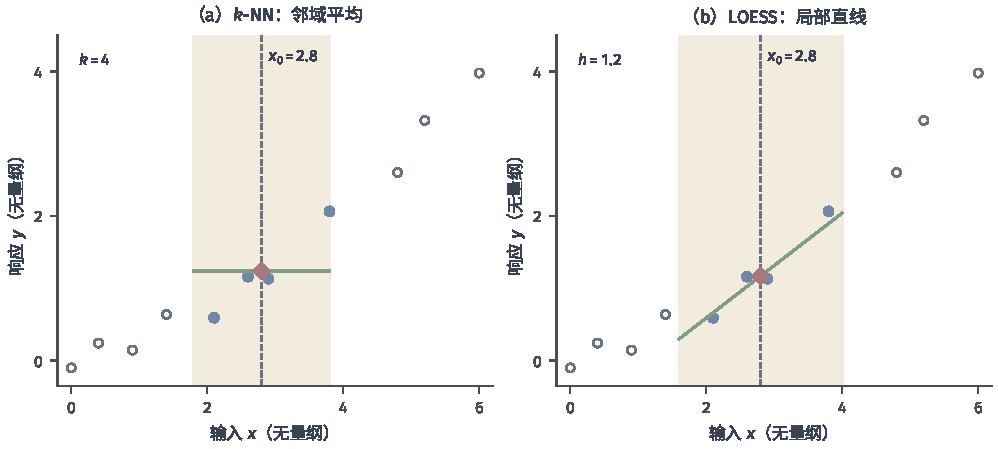
\includegraphics[width=159.059mm]{figures/04-classic-models/00-shared/matplotlib/regression-neighborhood/figure.pdf}
  \caption{同一查询点上的邻域平均与局部线性拟合。横、纵轴均无量纲，所有点均为构造样本；空心点为未使用样本，蓝色实心点为本次使用的四个样本，菱形为$x_0=2.8$处的预测。左图取$k=4$、等权平均，预测约为$1.238$；右图取$h=1.2$与三立方距离权重，不做残差重加权，局部线性预测约为$1.171$。浅色带标出各自的邻域，两图同时改变了局部函数形式和权重，不据此断言某种方法总是更准。}
  \label{fig:regression-neighborhood}
\end{figure*}

\subsubsection{参数学习}

设局部基设计为$\bm{P}$，权重矩阵为$\bm{W}=\operatorname{diag}(K_i)$。若$\bm{P}^{\top}\bm{W}\bm{P}$可逆，便可解加权正规方程得到局部系数；实际使用$\bm{W}^{1/2}\bm{P}$的QR分解等方法更合适。邻域无样本或有效点不足以确定多项式时，应扩大邻域、降低阶数或明确回退规则，不能直接使用逆矩阵公式。

一维局部线性形式可写得更清楚。令$u_i=x_i-x_0$，$S_j=\sum_iK_iu_i^j$、$T_j=\sum_iK_iu_i^jy_i$，并记$\Delta=S_0S_2-S_1^2$。方程组为
\[
  \begin{pmatrix}S_0&S_1\\S_1&S_2\end{pmatrix}
  \begin{pmatrix}\widehat a\\\widehat b\end{pmatrix}
  =\begin{pmatrix}T_0\\T_1\end{pmatrix}.
\]
若$\Delta>0$，查询点上的截距可表示为
\begin{equation}
  \widehat m(x_0)=\sum_i l_i y_i,\qquad
  l_i=\frac{K_i(S_2-u_iS_1)}{\Delta}.
  \label{eq:regression-local-linear-weights}
\end{equation}
对非负核权重，$\Delta=\sum_{i<j}K_iK_j(u_i-u_j)^2$，所以至少需要两个不同输入具有正权重。即使$\Delta>0$，接近退化的设计也可能产生很大的$l_i$。

固定带宽与只依赖输入的权重时，估计是响应$\bm{y}$的线性函数。若一个查询使用$n_{\mathrm{loc}}$个有效样本、$q$个局部基函数，稠密拟合约需$O(n_{\mathrm{loc}}q^2+q^3)$运算，另加邻域查询成本。

\subsubsection{局部斜率的作用与代价}
\label{sec:regression-loess-theory}

由式\eqref{eq:regression-local-linear-weights}求和可得$\sum_i l_i=1$、$\sum_i l_i(x_i-x_0)=0$。所以对于一次函数$m(x)=a+bx$，即使邻居都在查询的一侧，仍有$\sum_i l_i m(x_i)=m(x_0)$；局部斜率消去了平均输入不等于查询输入带来的一阶偏差。对光滑曲线，Taylor展开的常数项与一次项同样被再现，剩下的是曲率与更高阶变化。

这种补偿可能需要负权重。前面的两个单侧样本在$x_0=0$处给出$(l_1,l_2)=(2,-1)$，因此能从$0.1,0.2$外推到零。若两个响应分别含独立方差$\sigma^2$的噪声，局部线性预测方差为$(2^2+(-1)^2)\sigma^2=5\sigma^2$，等权平均则为$\sigma^2/2$。一般固定输入下，噪声方差为$\sum_i l_i^2\operatorname{Var}(Y_i\mid x_i)$；减少偏差可能增大方差，最终要由验证决定带宽与阶数\scite{fan1996local}。

\subsubsection{局部常数与稳健局部拟合}

\paragraph{用局部常数减少拟合参数}
\label{sec:regression-nadaraya-watson}

邻域中若只有一个有效输入，局部斜率无法确定；即使样本更多，估计斜率也可能带来不需要的噪声放大。只保留局部常数就能减少待估参数，同时保留按距离区别观测的方式。在式\eqref{eq:regression-local-polynomial}中只拟合截距，对截距求导便得到\term{Nadaraya--Watson核平滑}（Nadaraya--Watson kernel smoothing）
\begin{equation}
  \widehat m_{\mathrm{NW}}(\bm{x}_0)
  =\frac{\sum_iK_i y_i}{\sum_iK_i},
  \qquad \sum_iK_i>0.
  \label{eq:regression-nw}
\end{equation}
它与局部多项式使用相同的邻域权重，但只作加权平均。Nadaraya与Watson分别研究了这一核回归路线；具体带宽和设计条件仍须与所用理论结果对应\scite{nadaraya1964,watson1964}。

它保留非负权重与响应平均，计算比局部斜率简单；代价是不能自动抵消单侧邻域的线性趋势。局部常数、局部线性不是准确率的固定排序，而是不同局部信息与噪声下的取舍。

\paragraph{减弱异常响应对局部回归曲线的拉动}
\label{sec:regression-loess-robustness}

距离近不意味着响应可靠：查询附近的一条异常成交记录仍可能拉动整段拟合曲线。Cleveland的稳健LOESS先按距离作局部拟合，再根据残差增加降权系数，减小残差很大的记录在下一轮拟合中的作用。重复这两步后，局部曲线同时反映输入的远近和响应对当前曲线的偏离程度。

例如双权残差权重可取$a_i=[1-(r_i/c)^2]^2\mathbf1\{|r_i|<c\}$，其中$r_i=y_i-\widehat m(\bm x_i)$、$c>0$由残差尺度与验证设定。先在各训练输入处得到当前曲线与残差，算出$a_i$，再对每个查询将原距离权重改为$K_i a_i$，重新解局部加权问题。反复更新时检查局部秩和曲线变化，限制迭代次数；距离权重负责输入远近，残差权重负责当前拟合中的响应偏离，不能只算一次残差就声称已完成整个稳健过程。

残差权重依赖响应，整体估计便不再是固定的线性平滑算子，本节的固定权重方差公式不能直接沿用。这种处理针对异常响应；若局部输入覆盖不足，或异常输入支配了局部设计，残差降权本身不能补足信息。它也增加了重复拟合的计算成本，不能与只按输入设置带宽混为同一步骤。

\subsection{局部平均与局部拟合的关系}

$k$-NN用邻居数决定局部范围，距离加权和Nadaraya--Watson再区别邻居贡献；LOESS还在查询附近学习斜率或曲率。它们都保留训练记录参与预测，距离设定决定哪些记录提供依据，局部模型决定如何使用这些依据。搜索索引减少找邻居的工作，却不能代替LOESS每次查询的局部求解；稳健残差权重也不能补足没有数据的区域。

\section{基于树与规则的回归}
\label{sec:regression-trees}

第\ref{sec:classic-overview-tree-rules}节已经给出条件分支与区域预测的共同结构。本节关注回归时怎样按响应损失选择区域，并确定叶内预测。CART采用递归划分，模型树在叶内加入线性趋势，MARS用连续铰链基表达阈值及交互。MARS的基函数可以重叠，并不构成标准决策树；把它放在这里，是为了比较不同的条件与分段表达。

\subsection{CART 回归树}
\label{sec:regression-cart}

有些响应变化来自明确的条件组合，未必适合用全局直线或平滑邻域描述。考虑一个教学函数：只有$x_1>1/2$且$x_2>1/2$时响应为$10$，其他区域为$0$。固定$x_2\leq1/2$时，改变$x_1$不起作用；固定$x_2>1/2$时，越过$x_1=1/2$却使响应跳变。一个全局斜率无法同时表达这两种作用，平滑曲线也会在跳变附近折中。先按$x_2$分支，再在高值分支按$x_1$分支，就能用三个常数区域精确表示这个函数。

\term{分类与回归树}（classification and regression trees, CART）让数据选择这样的阈值与分支，并将递归二分、叶内估计和复杂度剪枝组织成统一框架。Breiman等人在1984年的专著中系统阐述了这套方法，把数据决定的分区与树的规模控制联系起来。回归情形通常用平方误差评价分裂，再通过独立验证选择树的规模；这一流程将在下面分别展开\scite{breiman1984cart}。

第\ref{sec:classification-cart}节的分类CART共享递归二分与代价复杂度剪枝。任务差异落在分裂和叶输出上：本节按响应平方误差选择分区并输出叶均值，分类树按类别不纯度或误分类代价分裂，并输出类别标签或类别比例。

\subsubsection{模型结构}

设树$T$的叶区域为$R_1,\ldots,R_M$，则
\begin{equation}
  f_T(\bm{x})=\sum_{m=1}^{M}c_m\mathbf{1}\{\bm{x}\in R_m\}.
  \label{eq:regression-cart-model}
\end{equation}
数值特征上的节点规则通常为$x_j\leq s$与$x_j>s$，递归后形成轴对齐区域；类别特征则可按类别子集分支，不宜继续称为普通欧氏矩形。缺失值并非由树结构自动解决，还需指定缺失方向或其他规则。例如，\term{替代分裂}（surrogate split）在主测试特征缺失时，用其他特征的测试尽量复现主分裂的左右分配。

固定非空叶的样本索引集$I_m$后，令$\bar y_m=|I_m|^{-1}\sum_{i\in I_m}y_i$，有
\[
  \sum_{i\in I_m}(y_i-c)^2
  =\sum_{i\in I_m}(y_i-\bar y_m)^2+|I_m|(c-\bar y_m)^2.
\]
因此$c_m=\bar y_m$在平方损失下最优。改用绝对或分位数损失时，叶预测相应变为中位数或分位数；模型结构与损失选择仍然可以分开。

图\ref{fig:regression-tree-prediction}把一棵给定的阈值树展开为预测函数。沿树走到同一叶的输入共享一个预测值，所以一维常数叶回归树产生水平分段，而阈值处可以跳跃。图中每个叶的数值都来自该叶的两条响应，后面的学习问题才是如何从候选阈值中选出这些分区。

\begin{figure*}[t]
  \centering
  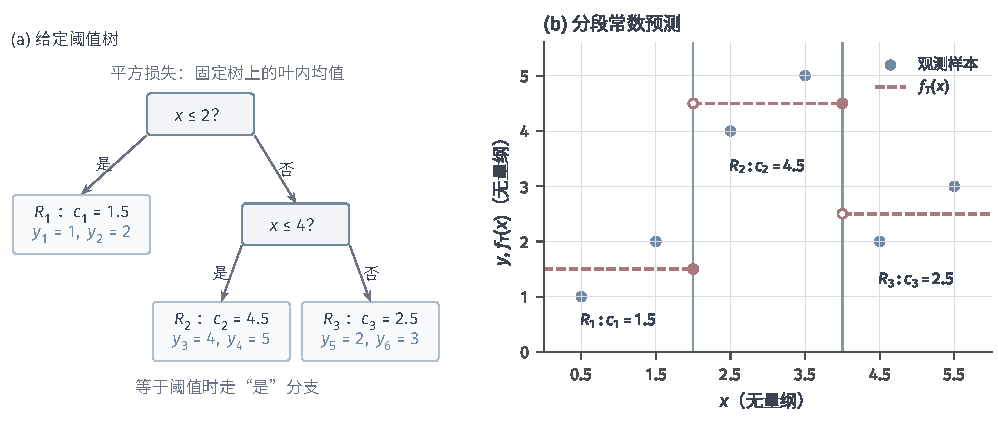
\includegraphics[width=159.059mm]{figures/04-classic-models/00-shared/matplotlib/regression-tree-prediction/figure.pdf}
  \caption{给定阈值树与分段常数预测。六个无量纲教学样本按$x$递增排列；按$x\leq2$及右分支上的$x\leq4$划分后，三组响应分别为$(1,2)$、$(4,5)$、$(2,3)$，叶均值为$1.5$、$4.5$、$2.5$。蓝色点表示样本，红色虚线表示预测，绿色竖线表示阈值；阈值处实心、空心端点区分取与不取该值。右图只显示$0\leq x\leq6$，树结构预先给定。}
  \label{fig:regression-tree-prediction}
\end{figure*}

\subsubsection{参数学习}
\label{sec:regression-cart-learning}

在当前节点内，算法枚举特征与候选阈值，选择子节点平方误差和最小的分裂。直观上，只要一个分裂能把响应均值明显不同的两群样本分开，让每群各自用自己的均值作预测，就比全体共用一个均值更贴合；若两群均值相同，分开就没有收益。对两个非空子节点，记样本数为$n_L,n_R$，均值为$\bar y_L,\bar y_R$，则分裂增益（父节点平方误差减去两个子节点平方误差之和）可精确写成
\begin{equation}
  \Delta_{\mathrm{split}}
  =\mathrm{SSE}_{\mathrm{parent}}
    -\mathrm{SSE}_{L}-\mathrm{SSE}_{R}
  =\frac{n_Ln_R}{n_L+n_R}(\bar y_L-\bar y_R)^2.
  \label{eq:regression-cart-gain}
\end{equation}
证明只需把两个子节点响应分别围绕自己的均值展开，再利用父均值为加权平均。该式说明增益同时考虑两组均值差异和样本量。

连续特征只需在相邻不同取值之间设候选切分，排好序后用累计和、平方和更新各侧SSE。类别子集有更多候选；在无额外分裂约束的平方误差二分问题中，可先按类别响应均值排序再考虑相邻分组，但带最小样本数、权重或其他限制时须重新检查相应结论。停止条件可限制最大深度、最小叶样本数和最低增益。贪心选择只保证当前节点在候选集中的最佳切分，不保证整棵树全局最优。

树一直生长下去，每片叶最终只剩一两个样本，训练误差可以降到零，但这只是把每条训练记录单独背下来，对新样本毫无意义。控制规模有两种时机：生长中途提前停止，或先让树充分长大、再回过头剪掉多余的分支。后者通常更稳妥——某些分裂单看一步收益很小，却能为下一步很有价值的分裂创造条件，提前停止会把这类结构一并错过；先长后剪则是在看到整棵树之后作全局取舍。固定一个已生长的有限二叉树$T_0$，用参数$\alpha$表示“每多保留一片叶需要付出的代价”，对其剪枝子树$T$定义
\begin{equation}
  R_\alpha(T)=\sum_{m\in\operatorname{leaves}(T)}
                    \mathrm{SSE}_m+\alpha|\operatorname{leaves}(T)|,
  \qquad\alpha\geq0.
  \label{eq:regression-pruning}
\end{equation}
$\alpha=0$时代价项为零，保留全部叶的大树最划算；$\alpha$增大，叶数多的树被罚得更重，更小的树逐渐成为最优，于是调节$\alpha$就能得到一列从复杂到简单的候选子树，再由验证集选出合适的规模。
\term{代价复杂度剪枝}（cost-complexity pruning）在保留局部拟合与减少叶数之间作折中。临界$\alpha$处可能出现多个最优子树，唯一性需要额外的并列规则。

\Needspace{11\baselineskip}
\begin{theorem}[CART在固定生长树内的最优剪枝解]
  \label{thm:regression-pruning}
  设$Q_\alpha(v)$为从$T_0$的节点$v$出发可得到的所有剪枝子树的最小代价。若$v$是原始叶，则$Q_\alpha(v)=\mathrm{SSE}_v+\alpha$；若$v$有左右孩子$v_L,v_R$，则
  \[
    Q_\alpha(v)=\min\{\mathrm{SSE}_v+\alpha,\,
                     Q_\alpha(v_L)+Q_\alpha(v_R)\}.
  \]
  从叶到根计算该递推，并保存每次选择，可得到$R_\alpha$的最优剪枝子树。
\end{theorem}

\begin{proof}
原始叶无其他选择，结论成立。对内部节点，任何合法剪枝子树要么把$v$收缩为一片叶，要么保留分裂。前者代价为$\mathrm{SSE}_v+\alpha$；后者的两个孩子可以独立剪枝，代价相加，归纳假设给出最小和为$Q_\alpha(v_L)+Q_\alpha(v_R)$。这两类穷尽全部选择，因此取最小值即可。相等时两个选择都最优，记录任一个并列规则均可返回一个最优解。
\end{proof}

固定$\alpha$时，递推只需对每个节点作常数次比较，因此在节点SSE已知后为$O(|T_0|)$。经典最弱环节方法进一步构造随$\alpha$变化的嵌套剪枝路径，再通过验证选择规模；它优化的仍是给定生长树内的剪枝集合，而不是所有可能的树。交叉验证时，各折的生长与剪枝都应仅使用该折训练集。

\subsubsection{分区选择与叶内趋势}
\label{sec:regression-cart-theory}

有限片常数适合表示阈值变化，却不擅长用少量叶描述连续斜率。例如$m(x)=1+2x$可由一个线性模型精确表示，常数叶必须继续切分才能逐渐逼近。另一方面，叶越来越小，估计其均值的记录也越来越少。树的深度、叶样本数和剪枝参数因此需要通过完整的训练—验证流程选择。

分裂使用了响应，不能在选完树后就把各叶当成事先固定的独立样本组，直接宣称叶均值无偏或方差只等于$\sigma^2/n_m$。独立数据分别选分区与估计叶均值，可以分离这两项选择，但普通CART并不自动具有这种安排。贪心分裂还可能错过需要联合考察的交互；后续Bagging、随机森林和提升树改变成员生成与组合，以处理不同的误差来源。

\label{sec:regression-model-tree}

如果区域内部仍有连续的线性变化，常数叶就需要继续切分。我们可以保留树对不同条件的分区，让每片叶负责拟合该区域内部的趋势。\term{模型树}（model tree）在叶内拟合线性模型$f_m(\bm{x})=b_m+\bm{w}_m^{\top}\bm{x}_{A_m}$，其中$A_m$为该叶使用的特征集。M5是这条路线的代表，用树选择适用区域，再用局部回归描述区域内部的趋势\scite{quinlan1992m5}。

固定分区后，第$m$片叶只用本叶记录最小化$\sum_{i:\bm x_i\in R_m}(y_i-b_m-\bm w_m^\top\bm x_{i,A_m})^2$，用OLS或带正则的线性求解得到系数；新输入先沿树找到叶，再计算该叶的线性预测。若分裂阶段就要按线性叶评价候选，可以对每个候选子区域分别重拟合叶模型，比较两侧总残差；此时不能继续把常数叶均值的式\eqref{eq:regression-cart-gain}当成该增益。分区、叶内特征与正则强度要和剪枝一起由训练内验证决定，不同模型树实现可采用不同搜索与平滑规则。

局部样本少时，叶内设计可能秩亏，需要选择变量或正则化。父子节点预测的加权混合可以缓和估计跳跃，但两侧叶模型在共同边界上没有被强制相等，因此这种平滑处理不自动保证函数连续。叶模型也可改为GLM、岭或Lasso，不过分裂准则、参数估计与复杂度惩罚需要与新模型配套，不能只替换叶公式就沿用全部CART理论。



\subsection{多元自适应回归样条（MARS）}
\label{sec:regression-mars}

树的阈值选择能够适应数据，常数叶却在边界处跳跃：跨过阈值的输入哪怕只差一点点，预测也会突然跳到另一个水平。很多真实关系并没有这种突变——比如价格随面积变化时，更常见的是斜率在某处发生改变，而不是价格整体跳一档。如果希望保留“阈值由数据自动确定”的好处，又让预测在跨过阈值时保持连续，可以让阈值处只改变之后直线的斜率，而不改变函数值本身。例如$m(x)=1+2x+3(x-1)_+$在$x\leq1$时斜率为$2$，在$x>1$时斜率为$5$；$(x-1)_+$在结点处从零开始增长，所以没有产生跳跃。常数叶需要许多区域来逼近这段线性变化，两个斜率和一个结点却已能准确描述它。\term{多元自适应回归样条}（multivariate adaptive regression splines, MARS）把阈值写进连续的铰链基函数，再从数据中选择这些基函数及其乘积。Friedman在1991年提出这一方法，将自适应选择结点与样条展开结合。它在可加模型与树式区域表达之间提供了另一种选择：多个基函数可同时作用于同一输入，预测不再由唯一一片叶决定\scite{friedman1991mars}。

\subsubsection{模型结构}

对特征$x_j$与结点$t$，\term{铰链函数}（hinge function）为$(x_j-t)_+$与$(t-x_j)_+$，它们在结点一侧为零，另一侧线性变化。MARS写成
\begin{equation}
  f(\bm{x})=\beta_0+\sum_{m=1}^{M}\beta_m B_m(\bm{x}),
  \qquad
  B_m(\bm{x})=\prod_{l=1}^{q_m}
                 [s_{m,l}(x_{j_{m,l}}-t_{m,l})]_+,
  \label{eq:regression-mars}
\end{equation}
其中$s_{m,l}\in\{-1,1\}$，$q_m$为该基的因子数。通常限制最高交互阶数，并对同一乘积中重复使用变量设规则，避免无约束扩张。下面采用每个乘积只使用互异变量的基本版本，因此$q_m$同时表示该基涉及的变量数；它不能超过预先给定的最高交互阶数$1\leq q_{\max}\leq d$。其他允许重复变量或平滑基的实现，需要另行说明自己的候选规则。

单个铰链连续但在结点不可微；含两个不同变量的乘积如$(x_1-3)_+(5-x_2)_+$在激活区域是二次乘积，不再是整体分段线性函数。铰链和乘积都连续，所以有限线性组合连续，但可微性需要额外平滑构造。严格加性版本只允许单变量基，增加乘积则允许指定阶数内的交互。

\subsubsection{参数学习}

前向阶段从常数模型开始，把已有基$B_l$与一对左右铰链相乘，尝试加入$B_l(\bm x)(x_j-t)_+$和$B_l(\bm x)(t-x_j)_+$。父基与其他已有基仍保留，区别于树用两个孩子替换一个叶。候选变量不能已出现在该乘积中，新增因子数不能超过$q_{\max}$；候选结点取父基非零区域内的不同训练取值，并要求结点两侧都有预定数量的观测支持。

对每个合法候选，都把新旧基一起组成设计矩阵，重新用QR或SVD拟合线性系数，再比较训练SSE。选取下降最多的一对后继续扩展，直到基数量达到上限、没有合法候选或改善不足。并列候选采用固定规则。比如父基为$(x_1-t_1)_+$时，在新变量$x_2$上扩展会增加只在$x_1>t_1$区域起作用的交互斜率；这个局部条件来自基的乘积，而不是唯一一条树路径。

后向阶段逐次尝试删除非截距基，每步保留训练误差增加最少的删除，形成由大到小的一串模型，并在每步重新拟合剩余系数。最后用验证误差或广义交叉验证选择规模。常用准则为

\begin{equation}
  \operatorname{GCV}
  =\frac{\mathrm{SSE}/n}{(1-C_{\mathrm{eff}}/n)^2},
  \qquad C_{\mathrm{eff}}<n.
  \label{eq:regression-mars-gcv}
\end{equation}
$C_{\mathrm{eff}}$是复杂度计数，既考虑保留的线性系数，也以附加惩罚近似结点搜索的代价。例如可写成$q+cK$，其中$q$是保留设计的秩，$K$是采用相应计数约定的结点数，$c$是每个结点的附加代价。软件对成对基、交互结点与自由度有不同计数方式，使用GCV前需要明确采用哪种复杂度计数；该计数近似了搜索代价，区别于自适应拟合的精确自由度。

\subsubsection{连续性、交互与搜索的边界}

增加结点能够改变单变量曲线的分辨率，增加乘积的变量数才能引入新的交互；两者不能互相替代。只允许单变量项时，MARS与GAM一样不能表达一般的$x_1x_2$作用；允许二阶乘积后，可以利用$x=(x)_+-(-x)_+$把这个交互展开为四个铰链乘积。固定基的系数拟合是最小二乘，选择哪些基却是离散的贪心搜索，局部改善不等于搜索全部结构后的全局最优。

结点和基由响应参与选择，GCV中的复杂度计数只是对搜索代价的近似，不能把被选中的基当作抽样前固定。应限制基数量和交互阶数，并用未参与搜索的验证记录比较。基本MARS连续但未必可微；铰链在观测范围外继续线性增长，外推需要另作检查。

\subsection{树、线性叶与铰链展开}

输入跨过阈值以后，预测可能切换到新的水平，也可能只改变斜率。CART用常数叶表达前一种情况；若区域内还有连续趋势，模型树在同一叶中增加线性项，减少为了描述斜率而继续切分的需要。MARS则把阈值写成连续铰链，允许多个基函数及其乘积共同作用于一个输入。模型树的不同叶仍可能在边界跳跃，MARS的基本构造连续但不必处处可微；前者按路径查询并估计各叶系数，后者计算保留的全部基。需要的局部样本、交互搜索和预测成本因而不同。

树的变量选择还可能偏向具有较多候选切分的特征。\term{条件推断树}（conditional inference tree）把变量关联检验与分裂位置选择分开，缓解候选切分多的变量更容易被选中的偏向；检验规则和显著性水平共同控制树大小，预测误差仍需由样本外评价确定\scite{hothorn2006ctree}。

\section{基于概率的回归}
\label{sec:regression-probabilistic}

一个房价点预测没有说明价格自身的波动，也没有说明有限数据下函数估计的差异。GLM已经通过条件分布描述前一种变化；本节进一步给未知系数或函数设置先验，由观测形成后验，再将函数不确定性与响应噪声一起带入预测分布。第\ref{sec:classic-overview-probabilistic}节的概率表示由此落实为可以计算的后验更新。

为什么需要把“函数”本身当作随机对象，而不只是估计一组固定系数？因为点预测给出的单个数值无法表达“这个预测有多可靠”：同一区域两套房屋可能给出相同的预测价格，但其中一处紧邻大量成交记录、估计很有把握，另一处远离任何观测、基本是在猜测，只看一个数字无法分辨二者。有限维基模型可以给系数设置分布来描述这种不确定性，但曲线形状从此被预先选定的基限死。如果希望直接用“相近输入处的函数值应当怎样一起起伏”来规定未知曲线的所有可能形状，就可以把概率模型建立在函数值上。

\subsection{高斯过程回归（GPR）}
\label{sec:regression-gpr}

点预测给出一个数值，却没有说明训练数据在该位置提供了多少信息。两个输入都得到相同价格预测，其中一个可能紧邻大量观测，另一个却远离训练范围；仅看这两个数值，无法分辨估计的不确定性。给有限基系数设置分布，可以描述未知系数带来的变化，但函数形状仍受预先选定的基限制。如果希望直接用“相近输入处的函数值怎样一起变化”来规定未知曲线，就可以把概率模型建立在函数值上。\term{高斯过程回归}（Gaussian process regression, GPR）用均值函数规定各位置的先验中心，用协方差函数规定函数值怎样共同变化。任意有限输入集合上的函数值都具有联合高斯分布，加入高斯观测噪声以后，可以精确计算后验与预测分布。先从有限权重模型推导这一计算，再转向函数值本身，就能看清它与贝叶斯线性回归、核岭回归的联系。

高斯过程预测较早已用于时间序列和地统计学，空间预测中的相关方法通常称为克里金（kriging）。20世纪90年代，Williams与Rasmussen在机器学习语境中讨论了GPR及协方差函数参数的学习，并将它与贝叶斯神经网络联系起来\scite{rasmussen2006}。

\subsubsection{模型结构}
\label{sec:regression-gpr-structure}

先考虑有限维特征$\bm\phi(\bm x)\in\mathbb R^p$，令$f(\bm x)=\bm\phi(\bm x)^\top\bm w$。OLS给出一组拟合系数，岭回归还会用惩罚规定哪些系数较可接受；如果要让预测保留这些未知系数的全部分布，而不是只保留一个点，就可以先设置系数的先验分布，再用观测更新。\term{贝叶斯线性回归}（Bayesian linear regression）采用这种做法。

考虑只含截距的教学模型。我们先给未知均值设置均值为$100$、方差为$20^2$的高斯先验，再将单次观测噪声的方差设为$10^2$。观测到一次$100$以后，后验均值仍是$100$，但后验方差从$400$降为$(1/400+1/100)^{-1}=80$。点预测没有变化，观测却减少了不确定性；预测下一次带噪响应时还要加上$100$的观测噪声方差。下面将这一计算推广到多个系数，使用高斯先验与高斯噪声通过完成平方求出后验。

这个方差更新可以直接从两个密度看出。若把未知截距记为$b$，先验密度与这一次观测的似然相乘，得到与$\exp\{-\tfrac12(b-100)^2(1/400+1/100)\}$成正比的后验密度。括号中的系数是方差的倒数，称为精度；它越大，密度越集中。这里先验和数据提供的精度相加，所以新的方差是精度之和的倒数。若观测值与先验中心不同，完成平方还会把中心改成按两种精度加权的平均。下面的矩阵公式保留相同机制：协方差的逆矩阵描述各参数方向的精度，观测通过设计矩阵提供额外信息。

\Needspace{14\baselineskip}
\begin{lemma}[贝叶斯线性回归的后验与预测]
  \label{thm:regression-bayesian-linear}
  条件于设计矩阵$\bm{X}$，设$\bm{w}\sim\mathcal{N}(\bm{m}_0,\bm{V}_0)$，其中$\bm{V}_0\succ0$，并设$\bm{y}=\bm{X}\bm{w}+\bm{\varepsilon}$，$\bm{\varepsilon}\sim\mathcal{N}(\bm{0},\sigma^2\bm{I})$与$\bm{w}$独立，$\sigma^2>0$。则
  \[
    \begin{aligned}
      \bm{V}_n&=(\bm{V}_0^{-1}+\sigma^{-2}\bm{X}^{\top}\bm{X})^{-1},\\
      \bm{m}_n&=\bm{V}_n
          (\bm{V}_0^{-1}\bm{m}_0+\sigma^{-2}\bm{X}^{\top}\bm{y}),
    \end{aligned}
  \]
  且$\bm{w}\mid\bm{X},\bm{y}\sim\mathcal{N}(\bm{m}_n,\bm{V}_n)$。新响应采用独立同方差噪声时，
  \[
    Y_{\star}\mid\bm{x}_{\star},\bm{X},\bm{y}
    \sim\mathcal{N}\bigl(
      \bm{\phi}_{\star}^{\top}\bm{m}_n,\,
      \bm{\phi}_{\star}^{\top}\bm{V}_n\bm{\phi}_{\star}+\sigma^2\bigr).
  \]
\end{lemma}

\begin{proof}
给定设计以后，后验密度正比于先验密度与似然的乘积。先保留两个二次项的原形，其负对数除去常数为
\[
 \tfrac12(\bm w-\bm m_0)^\top\bm V_0^{-1}(\bm w-\bm m_0)
 +\frac1{2\sigma^2}(\bm y-\bm X\bm w)^\top(\bm y-\bm X\bm w).
\]
第一项衡量参数偏离先验中心的程度，第二项衡量这些参数与观测的符合程度。分别展开这两个平方，把所有含$\bm w$的二次项和一次项合并，就得到下面的配方起点。
先验与似然的负对数相加，去掉与$\bm{w}$无关的项后为
\[
  \tfrac12\bm{w}^{\top}
       (\bm{V}_0^{-1}+\sigma^{-2}\bm{X}^{\top}\bm{X})\bm{w}
  -\bm{w}^{\top}
       (\bm{V}_0^{-1}\bm{m}_0+\sigma^{-2}\bm{X}^{\top}\bm{y}).
\]
定义引理中的$\bm{V}_n,\bm{m}_n$，上式等于
$\tfrac12(\bm{w}-\bm{m}_n)^{\top}\bm{V}_n^{-1}(\bm{w}-\bm{m}_n)$加常数。这是因为展开该平方后的一次项为$-\bm w^\top\bm V_n^{-1}\bm m_n$，而引理恰好令$\bm V_n^{-1}\bm m_n=\bm V_0^{-1}\bm m_0+\sigma^{-2}\bm X^\top\bm y$。先验精度正定，似然贡献的$\sigma^{-2}\bm X^\top\bm X$半正定，两者相加仍正定，故该可积密度归一化后就是所述高斯后验。新响应为后验高斯参数的线性变换与独立高斯噪声之和；线性变换的均值为$\bm\phi_\star^\top\bm m_n$、方差为$\bm\phi_\star^\top\bm V_n\bm\phi_\star$，再加上新噪声的方差即得预测分布。
\end{proof}

若只需用一个参数向量概括后验，可取当前参数化下的后验众数，即最大后验估计（MAP）。固定设计与超参数，且最大值能够取到时，当前回归模型的目标为
\begin{equation}
  \begin{aligned}
    \widehat{\bm{w}}_{\mathrm{MAP}}
      &\in\argmax_{\bm{w}}p(\bm{w}\mid\bm{X},\bm{y})\\
      &=\argmax_{\bm{w}}
        \{\log p(\bm{y}\mid\bm{X},\bm{w})+\log p(\bm{w})\}.
  \end{aligned}
  \label{eq:regression-map}
\end{equation}
后验的归一化常数与$\bm{w}$无关，因而不影响最大化。MAP使用后验众数，后验均值则对参数按后验加权平均，两者一般不同。

图~\ref{fig:regression-mle-map-geometry}在二维参数平面上展示这两个目标的差别。似然单独把最优点放在数据偏好的中心；零均值先验则偏好靠近原点的参数。MAP最小化负对数似然与负对数先验之和，因此落在二者共同决定的位置，而不是在MLE与先验中心之间任意作线性插值。椭圆形状和先验尺度改变时，折中的方向也会改变。
\begin{figure}[htbp]
  \centering
  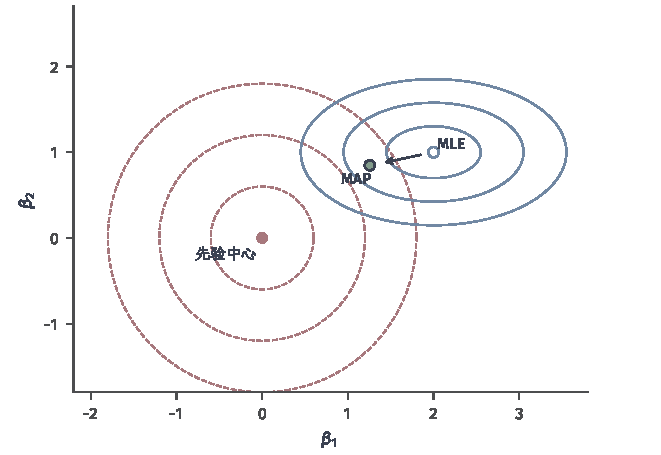
\includegraphics[width=105.412mm]{figures/04-classic-models/00-shared/matplotlib/regression-mle-map-geometry/figure.pdf}
  \caption{MLE与MAP的参数几何。蓝色实线是以$(2,1)^\top$为中心、两坐标尺度分别为$1$和$0.55$的高斯似然等高线；红色虚线是以原点为中心、尺度为$1.3$的各向同性高斯先验等高线。空心点为MLE，绿色实心点为两项相加后的MAP，坐标保留三位小数为$(1.257,0.848)^\top$。该构造用于显示先验如何改变点估计，不代表MAP总在两中心的连线上。}
  \label{fig:regression-mle-map-geometry}
\end{figure}

若$\bm{m}_0=\bm{0}$、$\bm{V}_0=\tau^2\bm{I}$，后验均值为$(\bm{X}^{\top}\bm{X}+\sigma^2\bm{I}/\tau^2)^{-1}\bm{X}^{\top}\bm{y}$，在本章归一化下对应$\lambda=\sigma^2/(n\tau^2)$的岭估计。高斯后验的均值与众数相同，所以也等于MAP估计。该对应要求截距处理一致：若先验惩罚全部特征系数，就不能直接与截距不受惩罚的岭模型比较。

后验协方差描述在当前先验与噪声模型中，观察数据后参数仍有多大不确定性；它不同于固定真参数、反复生成训练噪声时岭系数的协方差。高斯后验预测区间也依赖模型设定，不能直接当作任意真实函数下的覆盖保证。

有限维贝叶斯线性模型已经诱导出函数上的高斯分布：
\[
  m_0(\bm{x})=\bm{\phi}(\bm{x})^{\top}\bm{m}_0,\qquad
  k(\bm{x},\bm{x}')=\bm{\phi}(\bm{x})^{\top}\bm{V}_0\bm{\phi}(\bm{x}').
\]
任意有限个函数值都是高斯参数的线性变换，因此联合高斯。直接指定$m_0$和正定核$k$，便可越过显式系数建立函数先验。

把这一关系推广为$f\sim\mathcal{GP}(m_0,k)$：不再预先选定有限个基函数，而是直接对“任意位置上的函数值”规定一条概率律——在任意选取的有限个输入位置上，对应的函数值向量都服从联合高斯分布，其均值由$m_0$给定、任意两个位置之间的协方差由$k$给定。可以这样理解它：一条未知曲线在无穷多个位置上都有取值，我们无法把这无穷多个数都当成待估参数，但只需要保证“随便挑出有限个位置，它们的取值都服从一个由$m_0$和$k$决定的多元高斯”，整条曲线的随机规律就被完整规定了。同一个$m_0$和$k$保证删去或重排输入时，所得边缘分布彼此一致。核可以有限秩，因此贝叶斯线性回归正是一个特例；无限维核也只需通过有限函数值的联合分布计算，不必先列出无限多个权重。

加入与函数独立的噪声$y_i=f(\bm{x}_i)+\varepsilon_i$，其中$\varepsilon_i$相互独立且服从$\mathcal{N}(0,\sigma^2)$，$\sigma^2>0$。令$\bm{K}_{i,j}=k(\bm{x}_i,\bm{x}_j)$，$(\bm{k}_{\star})_i=k(\bm{x}_i,\bm{x}_{\star})$，$\bm{m}_0$表示训练点上的先验均值向量，$\bm{C}=\bm{K}+\sigma^2\bm{I}$，$f_{\star}=f(\bm{x}_{\star})$。联合分布为
\[
  \begin{pmatrix}\bm{y}\\f_{\star}\end{pmatrix}
  \sim\mathcal{N}\!\left[
    \begin{pmatrix}\bm{m}_0\\m_0(\bm{x}_{\star})\end{pmatrix},
    \begin{pmatrix}
      \bm{C}&\bm{k}_{\star}\\
      \bm{k}_{\star}^{\top}&k(\bm{x}_{\star},\bm{x}_{\star})
    \end{pmatrix}\right].
\]
于是后验预测可以精确写成
\begin{equation}
  \begin{aligned}
    \mu_{\star}
      &=m_0(\bm{x}_{\star})
        +\bm{k}_{\star}^{\top}\bm{C}^{-1}(\bm{y}-\bm{m}_0),\\
    v_{\star}
      &=k(\bm{x}_{\star},\bm{x}_{\star})
        -\bm{k}_{\star}^{\top}\bm{C}^{-1}\bm{k}_{\star}.
  \end{aligned}
  \label{eq:regression-gp-posterior}
\end{equation}
为证明它，令$Z=f_{\star}-m_0(\bm{x}_{\star})-\bm{k}_{\star}^{\top}\bm{C}^{-1}(\bm{y}-\bm{m}_0)$。直接计算得到$\operatorname{Cov}(Z,\bm{y})=\bm{0}$；$Z$与$\bm{y}$联合高斯，所以独立。其方差为$v_{\star}$，从而条件于$\bm{y}$时，$f_{\star}$的均值为$\mu_{\star}$、方差为$v_{\star}$。该方差非负也由它是随机变量方差得到。未来带噪声响应的方差则为$v_{\star}+\sigma^2$。



核选择规定了先验中的相似性。平方指数核$k(\bm{x},\bm{x}')=\sigma_f^2\exp(-\lVert\bm{x}-\bm{x}'\rVert_2^2/(2\ell^2))$具有很强的平滑性，其中$\sigma_f^2>0$是信号方差、$\ell>0$是长度尺度。Matérn核可调节平滑程度，例如$\nu=3/2$时为$\sigma_f^2(1+\sqrt3r/\ell)\exp(-\sqrt3r/\ell)$，其中$r=\lVert\bm{x}-\bm{x}'\rVert_2$，对应一次均方可微的过程。一维周期核可写成$\sigma_f^2\exp(-2\sin^2(\pi(x-x')/p)/\ell^2)$，表达周期$p>0$的相关结构。合法核的和与乘积仍合法，可以组合趋势与周期，但不保证所组合的结构符合实际数据。

这些参数规定函数值怎样共同变化：$\sigma_f^2$控制偏离先验均值的幅度，$\ell$越大，相同距离上的函数值相关性越强；平方指数核的两个位置相距$\ell$时，相关系数为$\exp(-1/2)$。它与第\ref{sec:classic-overview-common-kernels}节高斯核参数的对应为$\beta=1/(2\ell^2)$。Matérn核允许调整平滑程度，周期核则编码相隔$p$后反复出现的关系。核相加可以对应独立GP分量相加；核相乘仍合法，但不能据此把两个GP样本函数的乘积也称为GP。

图\ref{fig:regression-gp-posterior}展示了式\eqref{eq:regression-gp-posterior}的两项输出。在这个固定平稳核的例子中，观测附近的函数值受到较强约束，观测间的较大空隙与远离观测的区域保留更多不确定性。曲线给出点预测，带状区域则说明在当前先验和噪声设定下，哪些函数值仍与数据相容。

\begin{figure}[htbp]
  \centering
  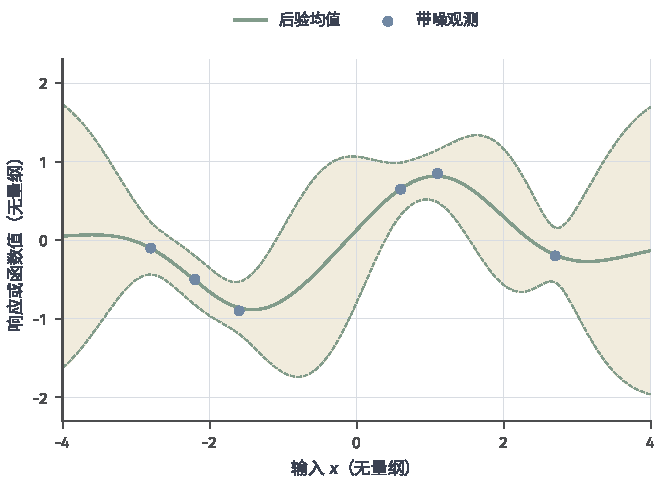
\includegraphics[width=105.412mm]{figures/04-classic-models/00-shared/matplotlib/regression-gp-posterior/figure.pdf}
  \caption{高斯过程的后验均值与函数不确定性。六个点为构造观测；先验均值为零，平方指数核取$\ell=0.9$、$\sigma_f=1$，观测噪声标准差为$\sigma=0.18$。实线为$\mu_{\star}$，浅色带及虚线边界为$\mu_{\star}\pm1.96\sqrt{v_{\star}}$，表示潜在函数值的逐点约$95\%$后验可信区间。它不是整条函数的同时可信带；预测未来带噪响应时，方差还须加$\sigma^2$。}
  \label{fig:regression-gp-posterior}
\end{figure}

\subsubsection{参数学习}
\label{sec:regression-gpr-learning}

给定核和噪声参数时，后验已经由式\eqref{eq:regression-gp-posterior}确定；仍需选择长度尺度、信号方差、噪声方差及可能的均值参数。为什么调这些超参数不能直接用训练拟合好坏，而要引入“边缘似然”？因为一条足够灵活的GP几乎可以穿过所有训练点，单纯追求拟合会把噪声方差调到零、长度尺度调到极小，得到一条剧烈振荡的曲线。合理的准则应当同时奖励“贴合观测”和“曲线本身平滑、不需要极端巧合”，边缘似然正好把这两点综合起来。令这些超参数为$\bm{\theta}$，把训练输入处的潜在函数值积分掉，得到\term{边缘似然}（marginal likelihood），即在给定输入和超参数时观测响应向量的概率密度——“积分掉”是指对先验允许的每一条可能的曲线，按它的先验概率加权，累加它产生当前观测的可能性，于是过于曲折、先验概率很低的曲线即使恰好穿过数据也不会占主导。以下令先验均值为零。
先把训练点上的潜在函数值记成$\bm f=(f(\bm x_1),\ldots,f(\bm x_n))^\top$，则这一积分写成
\[
 p(\bm y\mid\bm X,\bm\theta)
  =\int p(\bm y\mid\bm f,\bm X,\bm\theta)
         p(\bm f\mid\bm X,\bm\theta)\,d\bm f.
\]
积分中先按先验给每一组可能的函数值分配权重，再累加这些函数值产生当前观测的密度。零均值先验给出$\bm f\sim\mathcal N(\bm0,\bm K_{\bm\theta})$，独立高斯噪声与之相加，所以$\bm y\sim\mathcal N(\bm0,\bm C_{\bm\theta})$，其中$\bm C_{\bm\theta}=\bm K_{\bm\theta}+\sigma^2\bm I$。对这个$n$维高斯密度取对数，得到
\begin{equation}
  \log p(\bm{y}\mid\bm{X},\bm{\theta})
   =-\tfrac12\bm{y}^{\top}\bm{C}_{\bm{\theta}}^{-1}\bm{y}
    -\tfrac12\log|\bm{C}_{\bm{\theta}}|
    -\tfrac n2\log(2\pi).
  \label{eq:regression-gp-evidence}
\end{equation}
二次项评价响应与协方差结构的匹配，行列式项来自密度归一化，两者共同决定目标。行列式随核的尺度和相关结构变化，外层优化据此选择当前核族中的超参数；所选结构的预测效果仍需用样本外数据检查。

一维情形能说明为什么必须同时看这两项。若$Y\sim\mathcal N(0,c)$且$c>0$，去掉常数后的负对数密度为$y^2/(2c)+\log c/2$。单看第一项，增大$c$总能减轻非零观测的惩罚；但方差增大时，概率质量铺到更宽范围，当前位置的密度也会下降，这由第二项记录。多维公式在不同特征方向上作同样的权衡，不能只把二次残差压低就认定超参数更好。

学习超参数没有OLS那样的闭式解。我们可以计算边缘对数似然随每个超参数的变化，再沿增大它的方向迭代。固定零均值，记$\bm a=\bm C^{-1}\bm y$；对式\eqref{eq:regression-gp-evidence}关于$\theta_j$求导得到
\[
  \frac{\partial\log p(\bm{y})}{\partial\theta_j}
  =\tfrac12\operatorname{tr}\!\left[
    (\bm{a}\bm{a}^{\top}-\bm{C}^{-1})
    \frac{\partial\bm{C}}{\partial\theta_j}\right].
\]
它来自$d\bm{C}^{-1}=-\bm{C}^{-1}(d\bm{C})\bm{C}^{-1}$与$d\log|\bm{C}|=\operatorname{tr}(\bm{C}^{-1}d\bm{C})$。可以在正参数的对数坐标上使用梯度算法，多初值比较有助于发现不同局部最优；这种经验贝叶斯拟合通常仍把所选超参数当作固定值，因此没有保留全部超参数不确定性。



数值计算使用Cholesky分解$\bm{C}=\bm{L}\bm{L}^{\top}$。解两次三角方程得到$\bm{a}$后，预测均值为$\bm{k}_{\star}^{\top}\bm{a}$；令$\bm{v}=\bm{L}^{-1}\bm{k}_{\star}$，预测方差为$k(\bm{x}_{\star},\bm{x}_{\star})-\lVert\bm{v}\rVert_2^2$。稠密分解需要$O(n^3)$时间、$O(n^2)$存储，预计算后的单点均值需$O(n)$算术加核计算，单点方差通常需$O(n^2)$三角求解。均值与方差不能统称同一个预测代价。

\subsubsection{与贝叶斯线性回归和核岭回归的联系}
\label{sec:regression-gpr-theory}

有限基高斯权重产生有限秩GP，非线性核则可以直接规定更丰富的函数协方差。改变核改变允许的函数关系；改变观测似然才会改变响应分布。高斯噪声GP不能仅靠增加均值曲线的灵活性，精确表达两个相离峰的条件响应。

同一个零均值后验均值还可由\term{核岭回归}（kernel ridge regression）求得。在第\ref{sec:regression-svr-theory}节的核空间$\mathcal H_k$中，使用平方损失而不是SVR的容忍带损失：
\[
 \min_{f\in\mathcal H_k}
 \frac1{2n}\sum_i(y_i-f(\bm x_i))^2
       +\frac\lambda2\|f\|_{\mathcal H_k}^2,
 \qquad\lambda>0.
\]
数据项只看训练点值。将函数分成训练点核截面的线性组合与其正交余量后，再生关系使余量在训练点上为零，而范数平方多出余量的平方长度；删除余量不改变拟合却减小惩罚。因此最优函数可写成训练点核值的有限展开，其解为
\[
 \widehat f(\bm x)=\bm k_{\bm x}^\top\bm\alpha,
 \qquad\bm\alpha=(\bm K+n\lambda\bm I)^{-1}\bm y.
\]
即使$\bm K$奇异，$\lambda>0$也使移位矩阵正定，给出唯一函数解；不同系数仍可能表示同一函数。取$\lambda=\sigma^2/n$，就得到式\eqref{eq:regression-gp-posterior}的零均值GP后验均值。非零均值时先拟合$\bm y-\bm m_0$再加回$m_0$，额外的不受惩罚截距也必须单独处理。

这项等价只涉及点预测：核岭目标本身没有输出GP的后验方差。GP先验是随机函数的概率律，RKHS是确定性函数空间，无限维GP的样本曲线一般不属于其核的RKHS；后验均值具有核范数解释，不表示每条先验曲线都被限制在同一范数球中\scite{rasmussen2006}。

\subsubsection{非高斯响应：改变似然与近似后验}

\label{sec:regression-gp-nongaussian}

计数响应不能由连续高斯似然准确描述其取值范围。仍可设潜在函数服从GP，借助$\exp(f)$映射到条件均值，并按计数分布选择观测似然，但$p(\bm{f}\mid\bm{y})\propto p(\bm{y}\mid\bm{f})p(\bm{f})$一般不再是高斯，不能继续使用精确高斯回归公式。

例如，令$Y_i\mid f_i$服从均值为$\exp(f_i)$的Poisson分布，条件独立的观测给出$p(\bm y\mid\bm f)=\prod_i p(y_i\mid f_i)$。其对数似然含有$-\exp(f_i)$项，与高斯先验的二次对数密度相加后不再是二次函数。之前完成平方即可积分的步骤因此失效，近似推断要处理的是这一非高斯后验。

后验不再是高斯，也就没有现成的均值、方差公式。\term{拉普拉斯近似}（Laplace approximation）的思想是：先找到后验密度最高的位置（众数），再在该位置附近用一个高斯钟形去近似真实后验。之所以用高斯，是因为任意光滑单峰密度在峰顶附近的形状都近似钟形——峰顶处一阶导数为零，局部形状主要由二阶导数（曲率）决定，而高斯密度的对数恰好是二次函数。具体做法是在后验众数$\widehat{\bm{f}}$附近用二阶Taylor展开近似对数密度。若零均值先验的$\bm{K}$正定，并在众数处定义$\bm{W}=-\nabla^2\log p(\bm{y}\mid\bm{f})$，就可以先把未归一化的对数后验记为$g(\bm f)=\log p(\bm y\mid\bm f)-\bm f^\top\bm K^{-1}\bm f/2$。在内部可微众数处，梯度为零；令$\bm\delta=\bm f-\widehat{\bm f}$，二阶展开为
\[
 g(\bm f)\approx g(\widehat{\bm f})
       -\tfrac12\bm\delta^\top(\bm K^{-1}+\bm W)\bm\delta.
\]
对这个二次近似取指数，得到以$\widehat{\bm f}$为中心、以$\bm K^{-1}+\bm W$为精度矩阵的密度形状。将其归一化，后验局部高斯近似为
\[
  q(\bm{f})=\mathcal{N}\bigl(
       \widehat{\bm{f}},(\bm{K}^{-1}+\bm{W})^{-1}\bigr),
\]
前提是该精度矩阵正定。众数本身通常仍须通过Newton法等数值方法寻找，二阶近似并没有免除这个求解步骤。固定核时先迭代求众数和曲率，核超参数则可由相应的近似边缘似然或独立验证选择；外层选择必须和所用后验近似保持一致。若核有限秩，需在其有效子空间中计算；不能直接写不存在的$\bm{K}^{-1}$。多峰或强偏斜后验可能无法由一个局部高斯充分描述。



\term{变分推断}（variational inference）换一条路：不追求在众数附近作局部近似，而是在一个我们算得动的简单分布族（比如高斯族）里，挑出与真实后验“最接近”的一个分布来代替它。剩下的问题是怎样衡量两个分布的接近程度。为此引入\term{KL散度}（Kullback--Leibler divergence）：对相同基准测度下的密度$q,p$，在$q$为正处$p$也为正且相关期望存在时，$\operatorname{KL}(q\|p)=\mathbb E_q[\log(q/p)]\geq0$。它按$q$加权比较对数密度比，可以理解为“当真实分布是$p$、却用$q$来描述它时平均多付出的信息量”；它一般不对称（$\operatorname{KL}(q\|p)\ne\operatorname{KL}(p\|q)$），所以两个分布的位置不能交换，也不是通常意义上的距离。常用准则是最小化$\operatorname{KL}(q\|p(\bm f\mid\bm y))$，等价地最大化$\mathbb E_q[\log p(\bm y\mid\bm f)]-\operatorname{KL}(q\|p(\bm f))$；前一项奖励所选分布能解释观测，后一项把它向先验拉回。下面的诱导变量构造给出一种能降低计算量的分布族。

无论采用哪一种近似，都需先由近似后验得到测试位置的潜在预测分布$q(f_\star)$，再计算观测预测
\[
 p(y_\star\mid\bm X,\bm y,\bm x_\star)
   \approx\int p(y_\star\mid f_\star)q(f_\star)\,df_\star.
\]
潜在高斯的均值方差并不意味着观测响应也服从高斯；Poisson例中的积分给出计数概率，近似潜在后验和计算观测预测是相连的两个步骤\scite{rasmussen2006}。

\subsubsection{诱导变量：压缩后验计算}

\label{sec:regression-gp-computation}

稠密核矩阵的成本随样本数迅速增加：$n$个训练点要存$n^2$个两两核值、求解涉及$n^3$量级运算。回顾后验预测的形式，它只通过训练点与查询点之间的核值依赖数据，真正需要保存的是“这$n$条记录对未知曲线施加的全部约束”。如果曲线的主要起伏可以由少数$m$个位置上的函数取值来概括，那么其余位置的取值在给定这$m$个值后大体由核的相关结构决定，就不必为每一条训练记录维持同样规模的后验表示。

大数据下可选取$m\ll n$个输入位置$\bm{z}_j$，以潜在函数值$u_j=f(\bm{z}_j)$作为\term{诱导变量}（inducing variables），通过它们的近似后验概括数据对函数的约束。诱导位置可以取在训练输入之外，它们规定在哪里保留可调整的潜在函数信息，并不表示只留下这些位置附近的观测。

记诱导值向量为$\bm u$，训练点函数值向量仍为$\bm f$。原GP先验给出联合分布$p(\bm f,\bm u)=p(\bm f\mid\bm u)p(\bm u)$。选择一个可优化的$q(\bm u)$，并保留先验条件分布，构造
\[
 q(\bm f,\bm u)=p(\bm f\mid\bm u)q(\bm u),\qquad
 q(\bm f)=\int p(\bm f\mid\bm u)q(\bm u)\,d\bm u.
\]
这样把后验调整集中到$m$维的$\bm u$上，又通过条件分布把调整传到全部训练位置。即使给定$\bm u$，其余函数值通常仍有条件方差；该构造保留这部分随机性，没有把整条函数强行替换成由$m$个数确定的曲线。以下假设诱导核矩阵正定；若有重复位置或退化核，需先处理其有效子空间。

常用$q(\bm u)=N(\bm m_u,\bm S_u)$，待估的均值向量与协方差维数由$m$决定；可用$\bm S_u=\bm L_u\bm L_u^\top$保证协方差正定，$\bm L_u$取对角元为正的下三角矩阵。诱导位置、核参数和这些分布参数共同决定近似预测，而不只是在训练点中挑一个子集。

这个近似族对应的变分目标为
\[
 \mathcal L(q)
  =\mathbb E_{q(\bm f)}[\log p(\bm y\mid\bm f)]
    -\operatorname{KL}\{q(\bm u)\|p(\bm u)\}
  \leq\log p(\bm y\mid\bm X).
\]
在这个联合近似族中，$p(\bm f\mid\bm u)$在与先验比较时相消，所以KL惩罚只涉及诱导值分布。第一项仍利用全部$n$条观测衡量拟合，第二项惩罚诱导后验偏离其先验，以第一项减去第二项形成下界。其依据可以写成
\[
 \log p(\bm y\mid\bm X)-\mathcal L(q)
 =\operatorname{KL}\{q(\bm f,\bm u)
          \|p(\bm f,\bm u\mid\bm X,\bm y)\}\geq0.
\]
将KL中的后验按Bayes公式写成“似然乘先验再除以边缘似然”，并对$q$取期望，就得到这一恒等式。因此，固定模型时最大化下界，等价于在该近似族内减小与真实后验的KL距离。Titsias的变分诱导点方法在高斯回归中进一步利用这一目标选择诱导输入并近似后验，也可共同学习核参数；改变核参数时，边缘似然本身也随之改变\scite{titsias2009}。

学习时，固定核与诱导位置，先优化$\bm m_u,\bm S_u$以提高下界；高斯观测下这一步可解析完成，再对诱导位置和核参数优化所得下界。也可以用梯度迭代联合更新，但位置和核参数的外层目标仍可能有局部最优。对新输入，计算$q(f_\star)=\int p(f_\star\mid\bm u)q(\bm u)\,d\bm u$，再结合观测似然得到响应分布。先验条件分布把所学诱导后验传播到新位置，保留的条件方差也参与预测，不能把诱导均值直接当成无噪函数插值。

计算量的降低来自较小的矩阵规模。训练输入与诱导位置之间的核矩阵有$n\times m$个元素；形成相关的$m\times m$矩阵通常需要$O(nm^2)$运算，分解小矩阵另需$O(m^3)$。当$m\ll n$且采用稠密实现时，常把总规模写成$O(nm^2)$；存储相关交叉核矩阵需要$O(nm)$空间。后续随机变分方法进一步利用似然按记录分解的结构，以小批量估计目标的梯度。近似是否充分，仍需检查诱导表示能否保留任务所需的函数变化，尤其要分别核对点预测与方差估计的质量。

第\ref{sec:dim-gplvm}节的GPLVM复用GP核协方差和边缘似然，但把低维输入坐标也作为未知量。GPR从已观测输入预测响应，GPLVM则从高维观测反求低维坐标；二者共享概率函数表示，学习的对象与任务方向不同。

\subsection{后验预测与校准区间}

有限数据使系数或函数仍有不确定性，贝叶斯线性回归与GPR都用先验和观测形成后验。二者的区别在函数表示：前者用有限基系数，后者用核规定输入处函数值的共同变化；非线性基与有限秩核又使这两种表示相接。有限基的主要矩阵规模随基维数增长，稠密GPR的矩阵规模随训练样本量增长，诱导变量近似再用较少位置概括函数约束。选择时既要比较表示是否足够，也要区分只计算预测均值与还要计算方差的成本。

预测对象不同，也需要不同的不确定性描述。前面的后验区间有一个隐含前提：先验、核、噪声分布和超参数处理都设定正确，区间覆盖率才有概率意义；若这些假设与真实数据不符，名义上的$95\%$区间实际可能只覆盖远低于$95\%$的未来响应。共形方法提供了一条不依赖这些分布假设的补充路线：它不改变已训练好的任意预测器，只在其之外增加一个独立校准步骤，用一批没参与训练的留出记录观察“真实响应通常偏离预测多远”，再按观察到的偏离量为新预测配上一个半径。它们的构造与解释应分别核对，不能只按区间宽窄判断质量。若训练后冻结预测器，使用未参与拟合和选择的校准记录，且校准记录与未来记录可交换，共形方法可在相应构造下控制未来响应的边际漏覆盖概率；这不自动保证每个给定输入处的条件覆盖。覆盖条件及评价可参考\BookChapterRef{chap:trust-reliability}{卷三《基础、理论与可信性》的“可靠性”章}\scite{angelopoulos2022conformal,romano2019cqr}。

以绝对残差构造的分割共形区间为例。先冻结点预测器$\widehat f$，再取$N\geq1$条独立留出的校准记录，计算分数$s_i=|y_i-\widehat f(\bm x_i)|$。分数越大，表示该响应与预测越不相符。选定漏覆盖水平$0<\alpha<1$，令$k=\lceil(N+1)(1-\alpha)\rceil$；若$k\leq N$，取$N$个校准分数中第$k$小的值为$q$，若$k=N+1$，则取$q=+\infty$。对未来输入$\bm x_\star$报告
\[
 \mathcal C(\bm x_\star)
  =[\widehat f(\bm x_\star)-q,\,
    \widehat f(\bm x_\star)+q].
\]
排序位置使用$N+1$，是把未来分数与校准分数放在同一组可交换记录中比较；有并列值时，保留端点的区间规则给出保守覆盖。该保证平均校准记录与未来记录的随机性，控制边际覆盖，不自动保证每个给定输入的条件覆盖。若$k=N+1$，全实数区间虽保证覆盖，也表明校准数据不足以支撑所要求的有限宽度。它与GP区间的模型内后验概率是不同承诺。

若关心条件方差、偏度或尾部随输入怎样变化，第\ref{sec:regression-distributional}节的分布回归直接建模这些参数；若关心有限数据下函数估计的变化，则需要参数或函数后验。两种做法可以结合，却承担不同的建模选择：前者需指定响应分布族及各参数的输入结构，后者需指定先验、核与超参数处理。响应波动和函数估计不确定性因此需要分别检查。

\Needspace{6\baselineskip}
\section{本章小结}
\label{sec:regression-summary}

房价预测中的平均价格、预算阈值和价格分布，分别需要条件均值、条件分位数和分布信息。平方损失、分位数损失与概率似然规定不同目标，线性与核、邻域、树与规则则规定可用的函数表示。关系中缺少曲率或交互时，需要改变表示；数据难以分辨系数时，需要约束或压缩估计方向；异常响应影响过大时，需要调整残差的作用。扩展针对的环节不同，不能只按模型复杂程度排列。

% 本章共同的输出评价；原连续参数风险模板已按本轮模型讲解取舍移除。
各类回归输出在拟合、选择、校准与最终测试中的分工见表\ref{tab:regression-evaluation-protocol}。

\begin{table*}[htbp]
  \centering
  \small
  \begin{tabularx}{\linewidth}{@{}>{\RaggedRight\arraybackslash}p{22mm}>{\RaggedRight\arraybackslash}X>{\RaggedRight\arraybackslash}X>{\RaggedRight\arraybackslash}X@{}}
    \toprule
    输出 & 拟合与验证选择 & 独立校准 & 最终测试 \\
    \midrule
    条件均值 & 平方损失或均值模型似然；验证MSE & 点预测不另设 & MSE、残差与分组误差 \\
    条件分位数 & 对应$\tau$的损失；检查尾部记录与交叉 & 原始分位点不另设 & 分位数损失与经验超越率 \\
    模型内响应预测区间 & 拟合响应或后验模型；选择超参数 & 按模型构造；若再校准则单独留出 & 响应覆盖率、宽度与分组表现 \\
    共形覆盖区间 & 拟合基础预测器；校准前选定模型 & 留出记录估计不合格分数分位数 & 覆盖率、宽度与分组表现 \\
    完整分布 & 似然或适当评分；验证分布诊断 & 若作再校准则单独留出 & 负对数得分或CRPS、校准与锐度 \\
    \bottomrule
  \end{tabularx}
  \caption{不同回归输出的评价分工。两类区间均以未来响应为覆盖对象：模型内响应预测区间依赖其响应模型与参数估计或后验设定，共形覆盖区间用独立校准记录估计覆盖修正。最终测试留到模型选择与校准结束之后。}
  \label{tab:regression-evaluation-protocol}
\end{table*}

评价应与交付对象对应。在逐个比较指标之前，先要保证一件事：用来报告最终水平的数据，不能在模型训练或挑选时就被看过。因此一条记录在整个流程中要分工明确——拟合与选择超参数用训练折和验证折，共形区间另用独立校准记录，最后才用完全没参与任何选择的测试集报告结果；表\ref{tab:regression-evaluation-protocol}把这套分工按交付对象列清。在此基础上，条件均值比较测试均方误差（MSE），即残差平方的平均；分位数比较相应损失及经验超越率；未来响应区间同时报告覆盖率、宽度和分组表现。参数区间与潜在函数值区间覆盖各自的真值，不能直接拿带噪响应当条件均值真值。GP预测响应时应使用$v_\star+\sigma^2$，而不是只用函数方差$v_\star$。

完整分布可用\term{适当评分}（proper scoring rule）比较：在相关期望存在时，报告真实分布能取得最优期望评分。统一按损失越小越好计，负对数得分为$-\log p(y)$；给实际响应分配的概率或密度越低，损失越大。连续密度可以超过$1$，因此该得分不必非负。连续秩概率得分（continuous ranked probability score, CRPS）比较累积分布$F$与观测所给的阶跃函数：
\begin{equation}
 \operatorname{CRPS}(F,y)=\int_{\mathbb R}
        [F(t)-\mathbf1\{y\leq t\}]^2\,dt.
 \label{eq:regression-crps}
\end{equation}
有限一阶矩保证此积分有限，并保留响应单位；若$F$只在单点$a$取值，两个阶跃函数仅在$a$和$y$之间不同，积分就等于$|a-y|$。同均值、不同分散程度的分布可以获得不同评分，均值MSE不能替代整条分布的评价\scite{gneiting2007scoring}。

在房价任务中，先按部署时间或地区划分数据，每个训练折内完成缺失值处理、标准化、特征选择与拟合，再用验证结果选择表示和超参数。若需要共形覆盖区间，应在模型冻结后用独立校准记录确定修正，最后才用未参与选择或校准的测试集报告结果。看过测试结果后再调模型，该批数据便不再是最终测试证据。模型内区间是否需要另作校准，取决于交付要求，不由“报告区间”自动决定。


表示更灵活，需要更多数据分辨变化，也会增加计算与解释的成本。显式线性模型把训练信息压缩为系数，局部方法保留查询库，核方法的成本取决于展开规模与所需分布信息。应在同一验证流程下比较预测质量、存储、查询预算和解释需求，同时区分响应噪声、函数估计不确定性与区间覆盖各自回答的问题。

第\ref{chap:classification}章把数值响应换成类别标签，仍使用线性与核、近邻、分区和概率模型；任务改变后，输出、损失、邻域聚合与决策规则也随之改变。

\paragraph{扩展阅读}
Bishop教材第3、6章展开线性基函数、贝叶斯回归与核方法；Hastie等的教材比较正则化、局部回归与树回归，可进一步对照不同表示的误差和计算代价\scite{bishop2006,hastie2009}。

\chapter{分类}
\label{chap:classification}

判断邮件是否为垃圾邮件，需要从预设类别中作出选择。\term{分类}（classification）从带标签样本学习这种决策。设$D_n=\{(\bm{x}_i,y_i)\}_{i=1}^{n}$，$\bm{x}_i\in\mathbb{R}^{d}$、$y_i\in\{1,\dots,C\}$，分类器为$f:\mathbb{R}^{d}\to\{1,\dots,C\}$；预测类别发生变化的位置构成\term{决策边界}（decision boundary），边界一侧判为一类、另一侧判为另一类。本章讨论每个样本属于一个预设类别的单标签分类。

\emph{分类与回归的区别，以及本章的三种输出。}回归要预测的是可以连续取值的数值，分类要预测的是有限个离散类别，因此“差一点”的含义不同：把垃圾邮件判成正常邮件、或反过来，都是一次错误，错误没有“大小”之分，只有“对／错”两种结果。不过实际模型往往不只给一个硬邦邦的类别，而是分三个层次输出信息。最基础的是\emph{类别}：直接回答“是不是垃圾邮件”。进一步是\emph{得分}：给每一类一个实数，得分越高越倾向该类，按得分排序或与阈值比较就能得到类别——调整阈值可以改变“多严格才算垃圾邮件”。最丰富的是\emph{概率}：把得分归一化成各类的可能性，例如“是垃圾邮件的概率为$0.8$”，它除了能排序、定阈值，还能量化把握、计算不同决定的预期代价。同一个模型族可以在这三个层次上使用，但评价方式各不相同，本章会反复回到这一区分。

\emph{怎样衡量分类的好坏。}最直接的评价是数错了多少个：比较分类器时首先使用零一损失，预测标签与真实标签不同记为1，相同记为0。把它放到数据生成的角度，期望风险$R(f)=\mathbb P(f(\bm X)\ne Y)$衡量在与训练集同一分布的新样本上犯一次错的概率；我们无法直接计算它，因为真实分布未知，只能用训练记录上的错误比例，即经验风险$\widehat R_{01}(f)=n^{-1}\sum_i\mathbb 1\{f(\bm x_i)\ne y_i\}$来近似。“期望”与“经验”的差别，正是“未来可能犯多少错”和“手头这批数据错了多少”的差别，二者并不总是一致。除特别说明外，涉及这些风险的统计结论都假设训练样本独立同分布——各条记录彼此独立、且来自同一个分布——新样本也独立来自该分布。第\ref{sec:classification-lda-model}节先引出由真实类别后验决定的最小风险$R^\ast$，再区分这个理论基准与实际从有限数据估计出的分类器；训练目标中的对数损失、间隔损失等则分别在各模型处说明。

\emph{本章的组织线索。}同一批邮件可以有不同形式的类别证据，本章据此展开：把词频加权形成线性得分（LDA、感知机、SVM，第\ref{sec:classification-geometry}节）；让相似邮件提供局部标签（$k$近邻，第\ref{sec:classification-instances}节）；用词语的条件组合形成树或规则（第\ref{sec:classification-trees}节）；用概率模型比较各类后验（Logistic回归、朴素贝叶斯、GDA，第\ref{sec:classification-probability}节）。读这些节时可以注意，它们的输出形状（直线、局部投票、条件区域、概率）和学习准则（类统计量、错误反馈、间隔、信息增益、似然）是两件可以独立变化的事。半监督分类（第\ref{sec:classification-semisupervised}节）最后讨论一个现实问题：当真实标签昂贵、未标注文档却很多时，未标注输入在什么结构假设下能提供帮助。多个分类器组合成集成的内容放在第\ref{chap:ensemble-learning}章。

\section{基于线性关系的分类}
\label{sec:classification-geometry}

线性得分用特征的加权和比较类别：把各项证据加权相加成一个分数，分数为正判一类、为负判另一类，决策边界因此是一条直线（高维中是超平面）。这种形式简单、易解释，但它本身没有回答一个关键问题：权重从哪里来？本节考察三种完全不同的确定权重的依据：LDA先描述每类数据的分布（类均值与协方差），再由统计量推出权重；感知机不假设分布，直接根据分类错误一次次修正权重；SVM既不估计分布也不被动纠错，而是主动在众多能分开数据的直线中选一条离两边都最远的。三种方法最后得到的得分形式几乎一样，学到的边界却可能很不同。核方法随后把内积换成特征空间内积，使相同的间隔准则能够表达非线性关系；线性表示的基础见第\ref{sec:classic-overview-linear}节。

LDA兼有投影与概率解释：这里推导共享协方差形式及其扩展，第\ref{sec:classification-probability}节再从类条件分布的角度联系这些协方差约束与高斯NB。Fisher准则评价投影后的类统计量，感知机的有限更新保证依赖正间隔可分性，软间隔SVM则在目标中允许间隔违反。三者的条件分别服务于投影、更新和优化，比较时需要保留各自的对象。

\subsection{线性判别分析（LDA）}
\label{sec:classification-lda}

用花瓣长度与宽度区分两类鸢尾花时，只比较两类平均长度可能会遗漏宽度提供的信息。把两项测量相加也未必合适：如果某项测量在同类花之间就有很大波动，它对区分类别的作用可能不及另一项；两项测量相关时，还要考虑它们是否重复提供了同一份信息。我们需要据此确定各特征的权重，并选择划分类别的阈值。

一种办法是先描述每类测量值围绕中心怎样变化，再比较新样本来自各类的可能性。\term{线性判别分析}（linear discriminant analysis, LDA）在高斯生成模型下采用这条路线：类均值给出中心，共享协方差刻画类内尺度与相关性，类先验记录类别比例。由这些量计算的后验概率，最终给出一个线性判别函数。协方差相同是这里的建模假设，并非所有分类数据都具有的性质。

LDA还有一个几何起点。Fisher在1936年的鸢尾花分类研究中寻找一种线性组合，使两类均值的差异相对于类内波动尽可能大。这一准则不要求样本服从高斯分布；它与高斯生成模型可以给出相同的判别方向，但概率解释和适用条件有所不同\scite{fisher1936}。

从两类的线性组合转向多个总体的判别，问题不再只是选择一条轴，还包括需要保留多少个方向。Rao在1948年系统讨论了多总体的生物分类与判别表示，这也为理解LDA如何从分类规则延伸为有监督降维方法提供了历史背景\scite{rao1948}。

\subsubsection{模型结构}
\label{sec:classification-lda-model}

沿用训练集$D_n=\{(\bm{x}_i,y_i)\}_{i=1}^{n}$，其中$\bm{x}_i\in\mathbb{R}^{d}$、$y_i\in\{1,\ldots,C\}$。生成式LDA假设
\begin{equation}
  \label{eq:classification-lda-distribution}
  \begin{aligned}
    \mathbb{P}(y=c)&=\pi_c,\qquad \pi_c>0,\quad
      \sum_{c=1}^{C}\pi_c=1,\\
    p(\bm{x}\mid y=c)&=\mathcal{N}(\bm{x};\bm{\mu}_c,\bm{\Sigma}),
      \qquad \bm{\Sigma}\succ0 .
  \end{aligned}
\end{equation}
这里$\bm{\mu}_c\in\mathbb{R}^{d}$描述第$c$类的中心，$\bm{\Sigma}\in\mathbb{R}^{d\times d}$描述类内各方向的波动及特征之间的相关性。共享协方差允许各类具有不同中心，同时规定中心附近相同的椭球形状和朝向；协方差中的非对角元仍可表示特征相关性。

在零一损失下，应选择后验概率最大的类别。取对数并展开高斯密度，有
\begin{equation}
  \label{eq:classification-lda-score}
  \begin{aligned}
    \log\{\pi_c p(\bm{x}\mid y=c)\}
      &=a(\bm{x})+\delta_c(\bm{x}),\\
    \delta_c(\bm{x})
      &=\bm{x}^{\top}\bm{\Sigma}^{-1}\bm{\mu}_c\\
      &\quad-\frac12\bm{\mu}_c^{\top}\bm{\Sigma}^{-1}\bm{\mu}_c
        +\log\pi_c .
  \end{aligned}
\end{equation}
其中$a(\bm{x})$收集了$-\bm{x}^{\top}\bm{\Sigma}^{-1}\bm{x}/2$、对数行列式和高斯归一化常数，均与类别无关。正是共享协方差使二次项在类别比较时抵消，留下关于$\bm{x}$的仿射函数。任意两类得分相等的位置通常为超平面；多分类的各类别区域由这些两两比较共同确定。

训练后把估计参数代入$\delta_c$，得到$\hat{\delta}_c$。预测规则及相应的模型后验为
\begin{equation}
  \label{eq:classification-lda-prediction}
  \begin{aligned}
    \hat f_{\mathrm{LDA}}(\bm{x})
      &=\argmax_{c\in\{1,\ldots,C\}}\hat{\delta}_c(\bm{x}),\\
    \hat p_c(\bm{x})
      &=\frac{\exp\{\hat{\delta}_c(\bm{x})\}}
        {\sum_{j=1}^{C}\exp\{\hat{\delta}_j(\bm{x})\}} .
  \end{aligned}
\end{equation}
本节对$\argmax$的平局统一选择索引最小的类别。共享协方差也限定了LDA能利用的类别差异。例如，设两类中心都在原点，一类的测量值集中在中心附近，另一类的测量值分散得更开。此时“离中心有多远”包含类别信息，但LDA中两类相同的均值使与输入有关的得分项完全相消，分类只能依据先验比例。若两类先验还相等，按真实均值形成的这组得分处处平局，固定类别的预测错误率为$1/2$。这说明该参数选择丢掉了尺度信息；整个LDA候选空间的限制将在表达能力分析中讨论。

让每类使用自己的$\bm{\Sigma}_c$，就能把这种尺度差异保留下来。这得到\term{二次判别分析}（quadratic discriminant analysis, QDA），即允许二次决策边界的高斯分类器\scite{hastie2009}。例如两类协方差分别为不同倍数的单位矩阵时，后验比较包含到原点的距离平方，可以形成围绕中心的球形边界。QDA同时需要为每类估计协方差；每类样本较少时，新增的参数也可能使估计更不稳定。

\subsubsection{参数学习}
\label{sec:classification-lda-learning}

\paragraph{生成模型的最大似然估计}
有标签样本已经给出了每个观测所属的高斯分量，因此这里不需要推断类别归属。令$n_c=\sum_{i=1}^{n}\mathbb{1}\{y_i=c\}$，暂设各类都有样本。忽略与参数无关的常数，对数似然为
\begin{equation}
  \label{eq:classification-lda-likelihood}
  \begin{aligned}
    \ell
      &=\sum_{c=1}^{C}n_c\log\pi_c
        -\frac n2\log\det\bm{\Sigma}\\
      &\quad-\frac12\sum_{c=1}^{C}\sum_{i:y_i=c}
        (\bm{x}_i-\bm{\mu}_c)^{\top}
        \bm{\Sigma}^{-1}(\bm{x}_i-\bm{\mu}_c).
  \end{aligned}
\end{equation}
对先验加入约束$\sum_c\pi_c=1$，拉格朗日驻点给出$n_c/\pi_c$为同一常数；归一化后该常数为$n$。对$\bm{\mu}_c$求导，则有$\bm{\Sigma}^{-1}\sum_{i:y_i=c}(\bm{x}_i-\bm{\mu}_c)=\bm{0}$。由此得到
\begin{equation}
  \label{eq:classification-lda-mean-prior}
  \hat\pi_c=\frac{n_c}{n},\qquad
  \hat{\bm{\mu}}_c=\frac1{n_c}\sum_{i:y_i=c}\bm{x}_i .
\end{equation}
这两个估计分别是类别出现频率和该类的样本均值。

把均值代回似然，定义\term{类内散度矩阵}（within-class scatter matrix）
\begin{equation}
  \label{eq:classification-lda-within}
  \bm{S}_{\mathrm{W}}
    =\sum_{c=1}^{C}\sum_{i:y_i=c}
      (\bm{x}_i-\hat{\bm{\mu}}_c)
      (\bm{x}_i-\hat{\bm{\mu}}_c)^{\top}.
\end{equation}
它累加每个样本相对于本类中心的偏离。用精度矩阵$\bm{\Omega}=\bm{\Sigma}^{-1}$改写剩余目标，得到$n\log\det\bm{\Omega}/2-\operatorname{tr}(\bm{\Omega}\bm{S}_{\mathrm{W}})/2$。其驻点满足$n\bm{\Omega}^{-1}=\bm{S}_{\mathrm{W}}$，故当$\bm{S}_{\mathrm{W}}\succ0$时，
\begin{equation}
  \label{eq:classification-lda-covariance}
  \hat{\bm{\Sigma}}=\frac1n\bm{S}_{\mathrm{W}} .
\end{equation}
对$\bm{\Omega}$的目标是严格凹的，因此该驻点给出最大似然解。

式~\eqref{eq:classification-lda-covariance}的分母是$n$，不是$n-C$。这种合并各类类内变动的估计称为\term{合并协方差}（pooled covariance），其无偏形式为
\[
  \hat{\bm{\Sigma}}_{\mathrm{U}}
    =\frac{\bm{S}_{\mathrm{W}}}{n-C},\qquad n>C .
\]
在共享协方差假设下，给定各类样本数，有$\mathbb{E}[\bm{S}_{\mathrm{W}}\mid y_1,\ldots,y_n]=(n-C)\bm{\Sigma}$，因为估计每个类中心各消耗一个自由度。最大似然与无偏估计是不同准则；两种估计渐近相同，但有限样本下有所区别。特别是先验不等时，整体缩放协方差会改变几何得分相对于$\log\hat\pi_c$的权重，预测边界未必相同。

闭式估计把训练归结为统计量累计和线性代数运算。稠密数据的类内散度累计需要$O(nd^2)$运算，矩阵分解需要$O(d^3)$运算。实现时分解一次$\hat{\bm{\Sigma}}$，再解$C$个线性方程组$\hat{\bm{\Sigma}}\bm{a}_c=\hat{\bm{\mu}}_c$；预存$\bm{a}_c$与常数项后，每个样本的预测成本为$O(Cd)$。这些计算要求协方差可逆。$\bm{S}_{\mathrm{W}}$奇异时，正定参数域内的最大似然解不存在，需用降维或正则化重新规定估计问题。

\paragraph{Fisher投影的学习}
生成模型之外，还可以直接比较投影后的类间分离与类内波动。令总样本均值$\hat{\bm{\mu}}=\sum_c(n_c/n)\hat{\bm{\mu}}_c$，定义\term{类间散度矩阵}（between-class scatter matrix）
\[
  \bm{S}_{\mathrm{B}}
    =\sum_{c=1}^{C}n_c
      (\hat{\bm{\mu}}_c-\hat{\bm{\mu}})
      (\hat{\bm{\mu}}_c-\hat{\bm{\mu}})^{\top}.
\]
它衡量各类中心相对于总中心的分散程度。投影到方向$\bm{w}$后，两种散度分别变为$\bm{w}^{\top}\bm{S}_{\mathrm{B}}\bm{w}$和$\bm{w}^{\top}\bm{S}_{\mathrm{W}}\bm{w}$。\term{Fisher判别准则}（Fisher discriminant criterion）取两者之比。以下假设$\bm{S}_{\mathrm{W}}\succ0$，使每个非零方向的分母都为正：
\begin{equation}
  \label{eq:classification-fisher-criterion}
  J(\bm{w})
    =\frac{\bm{w}^{\top}\bm{S}_{\mathrm{B}}\bm{w}}
      {\bm{w}^{\top}\bm{S}_{\mathrm{W}}\bm{w}},
    \qquad \bm{w}\ne\bm{0}.
\end{equation}
分子鼓励类中心远离，分母抑制同类样本投影后过于分散。

图~\ref{fig:classification-lda-projection}固定同一组二维教学样本，只改变单位投影方向。两类中心分别为$(-1,0)^{\top}$与$(1,0)^{\top}$，每类都加上偏移$(-0.3,-1)^{\top}$、$(-0.1,1)^{\top}$、$(0.1,1)^{\top}$、$(0.3,-1)^{\top}$。由这些点算得$\bm{S}_{\mathrm{W}}=\operatorname{diag}(2/5,8)$与$\bm{S}_{\mathrm{B}}=\operatorname{diag}(8,0)$，最优方向由$\bm{S}_{\mathrm{W}}^{-1}(\hat{\bm\mu}_2-\hat{\bm\mu}_1)$归一化得到$\bm w^\ast=(1,0)^{\top}$。它使投影均值相差$2$，合并类内方差为$0.05$；比较方向$\bm w_{\mathrm B}=(3/5,4/5)^{\top}$的均值间距为$1.2$、类内方差为$0.658$，所以两者的$J$分别为$20$与$180/329$。这里方差按总样本量$8$归一化；右侧浅色条只是样本投影的最小至最大范围，不能把它当作Fisher准则中的平方偏差。

\begin{figure}[htbp]
  \centering
  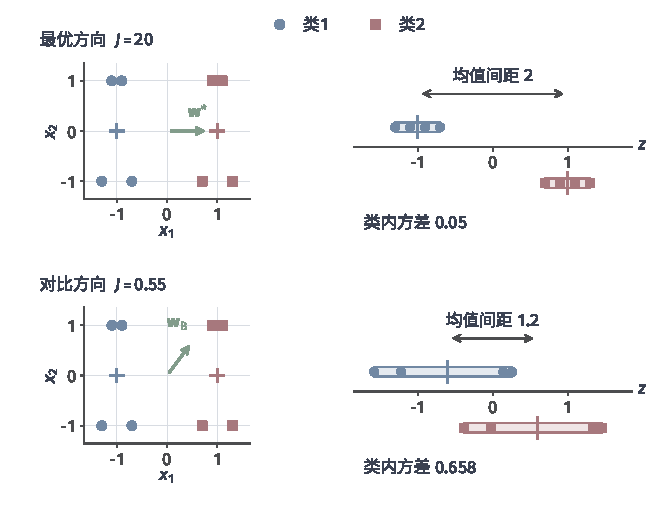
\includegraphics[width=112.000mm]{figures/04-classic-models/00-shared/matplotlib/classification-lda-target/figure.pdf}
  \caption{Fisher投影同时比较均值间距与类内散布。每类4个教学点，坐标无量纲；两行复用同一点集和相同投影数轴尺度。左侧绿色箭头为单位投影方向，十字为类均值；右侧短竖线为投影均值，浅色条为各类的样本投影范围，双向箭头标出均值间距。标注方差由$n^{-1}\bm w^{\top}\bm S_{\mathrm W}\bm w$计算，$J$仍按散度比计算。}
  \label{fig:classification-lda-projection}
\end{figure}

由于$J$不受$\bm{w}$的非零倍数缩放影响，可以约束$\bm{w}^{\top}\bm{S}_{\mathrm{W}}\bm{w}=1$。对$\bm{w}^{\top}\bm{S}_{\mathrm{B}}\bm{w}-\lambda(\bm{w}^{\top}\bm{S}_{\mathrm{W}}\bm{w}-1)$求导，得到\term{广义特征值问题}（generalized eigenvalue problem）：
\begin{equation}
  \label{eq:classification-fisher-eigenproblem}
  \bm{S}_{\mathrm{B}}\bm{w}
    =\lambda\bm{S}_{\mathrm{W}}\bm{w}.
\end{equation}
驻点还需比较大小。令$\bm{v}=\bm{S}_{\mathrm{W}}^{1/2}\bm{w}$，则
\[
  J(\bm{w})=\frac{\bm{v}^{\top}\bm{A}\bm{v}}{\bm{v}^{\top}\bm{v}},
  \qquad
  \bm{A}=\bm{S}_{\mathrm{W}}^{-1/2}
    \bm{S}_{\mathrm{B}}\bm{S}_{\mathrm{W}}^{-1/2}.
\]
把$\bm{v}$展开到对称半正定矩阵$\bm{A}$的正交特征向量上，上式就是各特征值的加权平均，权重非负且总和为$1$。最大值因而是最大特征值；取对应特征向量，再乘$\bm{S}_{\mathrm{W}}^{-1/2}$，便得到最优Fisher方向。若最大特征值有重数，最优方向未必唯一。

二分类时，令$\bm{h}=\hat{\bm{\mu}}_1-\hat{\bm{\mu}}_2\ne\bm{0}$，由总均值的定义可得
\[
  \bm{S}_{\mathrm{B}}=\frac{n_1n_2}{n}\bm{h}\bm{h}^{\top},
  \qquad
  \bm{w}_{\mathrm{F}}\propto\bm{S}_{\mathrm{W}}^{-1}\bm{h}.
\]
生成式LDA的法向量则为$\bm{w}_{\mathrm{G}}=\hat{\bm{\Sigma}}^{-1}\bm{h}=n\bm{S}_{\mathrm{W}}^{-1}\bm{h}$，两者方向相同。但完整的生成式分类规则还比较
\begin{equation}
  \label{eq:classification-lda-binary-threshold}
  \hat\delta_1(\bm{x})-\hat\delta_2(\bm{x})
    =\bm{w}_{\mathrm{G}}^{\top}
      \left(\bm{x}-\frac{\hat{\bm{\mu}}_1+\hat{\bm{\mu}}_2}{2}\right)
      +\log\frac{\hat\pi_1}{\hat\pi_2}
\end{equation}
的正负。Fisher准则本身只给方向，不给类先验、后验概率或这一阈值。两类均值相同时，均值散度准则没有正特征值方向，而生成模型仍可按先验选择类别。因此Fisher投影可用于非高斯数据，而贝叶斯最优性的证明还需要正确指定的高斯生成模型。

\subsubsection{理论分析}
\label{sec:classification-lda-analysis}

\paragraph{表达能力}
若真实类条件分布满足式\eqref{eq:classification-lda-distribution}，其后验概率就属于LDA的候选概率函数集，相应的贝叶斯决策也属于候选分类规则，无须用近似模型代替。共享协方差允许相关特征和不同类中心，但规定各类只有一个高斯峰，且峰周围的形状相同。即使不把得分解释为高斯后验，两个仿射得分的比较也只能产生一个半空间，不能表达任意形状的类别区域。

前面的同中心例子可以具体写成两类等先验、均值均为零，协方差分别为$\sigma_1^2\bm I_d$与$\sigma_2^2\bm I_d$，其中$0<\sigma_1<\sigma_2$。比较真实高斯密度得到：类1的贝叶斯区域是
\[
  \|\bm x\|_2^2<r_0^2,
  \qquad
  r_0^2=\frac{2d\log(\sigma_2/\sigma_1)}
                   {\sigma_1^{-2}-\sigma_2^{-2}}.
\]
小方差类在中心附近占优，大方差类在外侧占优。LDA的每个二类候选规则都以半空间作为类别区域，因而无法重现这个有界球。QDA保留半径平方项，候选空间能够表达这里的目标区域；两者的区别落在得分中是否允许这项二次关系。

\paragraph{收敛性}
固定训练集、各类别非空且类内散度正定时，生成式LDA的闭式参数达到该高斯模型的经验似然全局最大值，不需要迭代搜索。累积散度约需$O(nd^2)$运算，分解协方差约需$O(d^3)$运算；奇异情形没有这一正定域内的有限最优解。Fisher投影则通过广义特征值求解达到其比值准则的全局最大值，数值精度与矩阵条件数有关。

\paragraph{泛化性}
闭式估计只解决当前训练集上的拟合。下面先证明参数估计的\term{一致性}（consistency），再说明这些参数构成的分类器能否接近贝叶斯风险。给定训练集$D_n$后，$R(f\mid D_n)$只对独立新样本取平均。

\begin{lemma}[LDA参数估计的一致性]
  \label{thm:classification-lda-consistency}
  设$d$和$C$固定，训练样本独立同分布，真实分布满足式~\eqref{eq:classification-lda-distribution}，且所有$\pi_c^\ast>0$、$\bm{\Sigma}^\ast\succ0$。当$n\to\infty$时，
  \[
    \hat\pi_c\xrightarrow{\mathbb{P}}\pi_c^\ast,\qquad
    \hat{\bm{\mu}}_c\xrightarrow{\mathbb{P}}\bm{\mu}_c^\ast,\qquad
    \hat{\bm{\Sigma}}\xrightarrow{\mathbb{P}}\bm{\Sigma}^\ast .
  \]
  所有类别非空且$\hat{\bm{\Sigma}}$正定的概率趋于$1$。
\end{lemma}

\begin{proof}
  为处理随机的$n_c$，把类均值写成两个全样本平均之比：
  \[
    \hat{\bm{\mu}}_c
      =\frac{n^{-1}\sum_{i=1}^{n}\bm{x}_i\mathbb{1}\{y_i=c\}}
        {n^{-1}\sum_{i=1}^{n}\mathbb{1}\{y_i=c\}} .
  \]
  大数定律使分母收敛到$\pi_c^\ast>0$，分子收敛到$\pi_c^\ast\bm{\mu}_c^\ast$，因而先验和均值都一致。尚未观察到某一类时可以任意约定其均值；该事件的概率趋于零，不影响结论。

  共享协方差估计可展开为
  \[
    \hat{\bm{\Sigma}}
      =\frac1n\sum_{i=1}^{n}\bm{x}_i\bm{x}_i^{\top}
        -\sum_{c=1}^{C}\hat\pi_c
          \hat{\bm{\mu}}_c\hat{\bm{\mu}}_c^{\top}.
  \]
  高斯分布有有限二阶矩，故第一项收敛到
  \[
    \mathbb{E}[\bm{x}\bm{x}^{\top}]
      =\bm{\Sigma}^\ast+
        \sum_{c=1}^{C}\pi_c^\ast
          \bm{\mu}_c^\ast(\bm{\mu}_c^\ast)^{\top}.
  \]
  第二项消去类中心对二阶矩的贡献，余下$\bm{\Sigma}^\ast$。固定维数下，矩阵逐元素收敛也给出算子范数收敛；由$\bm{\Sigma}^\ast$的最小特征值严格为正，估计矩阵以趋于$1$的概率可逆。上述步骤实际上可由强大数定律加强为几乎必然收敛。
\end{proof}

矩阵求逆和$\log\pi_c$在这些条件下连续，所以在参数几乎必然收敛的事件上，对每个固定输入$\bm{x}$，有$\hat\delta_c(\bm{x})\to\delta_c^\ast(\bm{x})$。但$\argmax$在平局处不连续：在真实最大得分唯一的输入处，估计类别最终等于该输入的唯一贝叶斯类别；平局处则未必如此。若最优类别平局的输入集合概率为零，就能进一步推出随机输入上的预测标签收敛。不同贝叶斯分类器在平局处可以选择不同标签，却有相同风险。

参数收敛怎样传到预测错误率，可以直接通过类别后验比较，因而不需要排除后验平局。
\begin{theorem}[LDA在高斯同协方差条件下的期望分类风险界]
  \label{thm:classification-lda-risk}
  在引理\ref{thm:classification-lda-consistency}的条件下，用闭式估计的先验、均值和共享协方差构造$\hat p_c$，返回$\hat f_{\mathrm{LDA}}=\argmax_c\hat p_c$，平局按固定类别次序处理。不能拟合的训练集上暂用任意固定分类器。记真实后验为$p_c^\ast$，则在估计模型有定义时，
  \[
    0\leq R(\hat f_{\mathrm{LDA}}\mid D_n)-R^\ast
      \leq2\mathbb E_{\bm X}
        \max_c|\hat p_c(\bm X)-p_c^\ast(\bm X)|.
  \]
  随$n\to\infty$，左侧几乎必然趋于零，而且
  $\mathbb E_{D_n}R(\hat f_{\mathrm{LDA}}\mid D_n)\to R^\ast$。
\end{theorem}
\begin{proof}
记$f^\ast$为任意贝叶斯规则。由于$\hat f_{\mathrm{LDA}}$最大化$\hat p_c$，逐点有
\begin{equation}
  \label{eq:classification-lda-excess-risk}
  \begin{aligned}
    0&\leq p_{f^\ast(\bm{x})}^\ast(\bm{x})
      -p_{\hat f_{\mathrm{LDA}}(\bm{x})}^\ast(\bm{x})\\
      &\leq 2\max_{1\leq c\leq C}
          |\hat p_c(\bm{x})-p_c^\ast(\bm{x})| .
  \end{aligned}
\end{equation}
这个上界来自在两项之间分别加减相应的估计后验，并利用$\hat p_{\hat f_{\mathrm{LDA}}}\geq\hat p_{f^\ast}$。对独立测试输入积分，左侧成为超额风险，得到定理中的不等式。在参数几乎必然收敛的事件上，后验估计对每个输入收敛，右端的被积函数趋于零且不超过$2$；支配收敛定理给出条件风险的极限。再用风险位于$[0,1]$，对训练集取期望即可得到最后一个结论。由参数一致性引理，不能拟合的事件几乎必然最终不再出现。
\end{proof}

这条推理从训练统计量出发，经后验误差控制到独立新样本风险，依赖正确指定的高斯模型与固定维数。它给出风险极限，未给出有限样本速率；维数随样本量增长时也需另外分析。Fisher准则只评价投影的散度比例，没有这些分布条件时，不能由它推出上述风险结论。

\subsubsection{优化表达能力}

\paragraph{允许各类具有不同协方差}
\label{sec:classification-lda-covariance-extensions}
如果不同类别的类内变化方向和尺度明显不同，共享协方差就会限制LDA的表达能力。第\ref{sec:classification-lda-model}节已经定义的二次判别分析（QDA）保留类条件高斯假设，却为每个类别估计独立的协方差矩阵$\hat{\bm{\Sigma}}_c$。先假设各类协方差估计均正定，删去各类共同的常数项后，其判别得分为
\begin{equation}
  \begin{aligned}
    \delta_c(\bm{x})
      ={}&\log\hat{\pi}_c-\frac12\log\det\hat{\bm{\Sigma}}_c\\
        &-\frac12(\bm{x}-\hat{\bm{\mu}}_c)^\top
          \hat{\bm{\Sigma}}_c^{-1}(\bm{x}-\hat{\bm{\mu}}_c).
  \end{aligned}
  \label{eq:classification-qda-score}
\end{equation}
任意两类得分之差含有关于$\bm{x}$的二次项，所以边界一般是二次曲面。当协方差相同时，二次项相消，又得到 LDA。增加自由度也增加了估计负担：共享协方差模型需要$O(d^2+Cd)$个参数，QDA 则需要$O(Cd^2)$个参数；每一类只有少量样本时，独立协方差容易不稳定甚至奇异。第\ref{sec:classification-gda}节将从生成分布的角度统一这两种模型。

\paragraph{支持非线性关系}
\label{sec:classification-lda-kernel-extension}
QDA通过类协方差的差异产生二次边界；Fisher判别则可以从输入表示入手，改变只作线性投影的限制。例如，内外两圈样本在原坐标中的均值都可能接近原点，原坐标上的均值差便提供不了有用方向；增加距离平方等非线性特征后，两类在新坐标中可以具有不同均值。Mika等提出的\term{核 Fisher 判别}（kernel Fisher discriminant, KFD）在特征空间中重新计算类均值与散度，再最大化投影后的类间与类内散度比\scite{mika1999kernel}。
将投影方向写成$\bm{w}=\sum_{i=1}^n a_i\phi(\bm{x}_i)$，两种投影散度就都能写成系数$\bm{a}$与核矩阵构成的二次型，目标仍是它们的比值；类内散度的奇异性则用正则化处理。它与核 SVM 的区别仍在训练准则：KFD 关注整体类统计量，SVM 关注间隔及其违反程度。KFD 的基本解通常没有支持向量式的稀疏性，预测可能需要访问全部训练样本；若要从投影得分得到后验概率，还需额外建立得分分布或校准模型。
例如，内外两圈分别具有固定半径$1$与$2$时，径向特征$\phi(\bm x)=\|\bm x\|_2^2$把两类送到$1$与$4$。在二者之间设置阈值就能精确分开，带正则化的类内散度也不妨碍这个得分表示。若所选核仍只提供原坐标的线性组合，同中心两圈的均值差仍为零，Fisher准则便没有得到所需的径向信息。所选核是否保留径向信息，决定了这里的目标能否表达。

\subsubsection{优化泛化能力}

QDA放开了各类的形状，但少数类可能没有足够样本估计完整协方差。例如，一个类别只有10个样本，中心化后的样本协方差秩至多为9；若输入有20维，这个估计便无法求逆。完全改用LDA又会舍弃类间真实的尺度或方向差异。可以在两者之间折中，让各类借用一部分合并统计量。\term{正则化判别分析}（regularized discriminant analysis, RDA）通过收缩协方差控制这种取舍。Friedman的原始方法包含两个调节方向：将类内协方差向合并协方差收缩，再向球形协方差收缩\scite{friedman1989rda}。
记$n_c$为第$c$类样本数，$\hat{\bm{\Sigma}}$为以$n$为分母的合并协方差。一种与原始构造相符的写法是
\begin{equation}
  \begin{aligned}
    \bm{A}_c(a)
      &=\frac{(1-a)n_c\hat{\bm{\Sigma}}_c+an\hat{\bm{\Sigma}}}
              {(1-a)n_c+an},\\
    \tilde{\bm{\Sigma}}_c(a,b)
      &=(1-b)\bm{A}_c(a)
        +b\,\frac{\operatorname{tr}\bm{A}_c(a)}{d}\bm{I},
        \qquad a,b\in[0,1].
  \end{aligned}
  \label{eq:classification-rda}
\end{equation}
当$b=0$时，$a=0$与$a=1$分别对应 QDA 与 LDA 的协方差估计；增大$b$会减弱各方向方差差异，并在平均方差为正时帮助获得可逆估计。两个参数应在训练集内部通过验证选择。当合并协方差和各类协方差均奇异时，可逆性还需要平均方差为正的球形收缩项或其他正则化。

收缩也改变哪些类别差异能够进入得分。$a=1,b=0$时各类共享协方差，二次项相消；$b=1$时每类协方差都为单位矩阵的一个倍数，得分可以利用半径平方，却不能独立利用各方向的方差与特征相关性。只有保留完整的类特有协方差，才能表达前面QDA中的一般二次差异。RDA是在这些限制与估计波动之间选择，不是一个可以越过QDA分布族的新模型。

收缩强度越大，类形状越受限制；强度越小，越依赖每类样本估计完整协方差。应在训练数据内部选择强度，再检查独立数据上的分类误差与估计稳定性。

\subsubsection{小结}
\label{sec:classification-lda-summary}

LDA把类中心、类内波动与类别比例合成一个得分。共享协方差使两类比较中的二次项抵消，留下线性边界；高斯生成模型还给出后验与阈值。Fisher的投影准则则把均值分离和类内散布放在同一个比值中，适合解释各特征怎样参与判别，但只选方向，不能独自给出后验概率。

类形状不同时，QDA保留各类协方差，代价是每类都要有足够数据支持矩阵估计。小样本、高维条件下，Friedman的RDA让各类借用合并统计量，再按需要向球形协方差收缩，减轻独立估计的波动。收缩越强，能够保留的方向与尺度差异越少；收缩参数的选择也增加了验证工作。

另一类困难来自原坐标没有显示类别差异。内外两圈的均值可以相同，单纯调整协方差估计无法为线性Fisher投影补上径向关系。Mika等的核Fisher判别把类统计量移到特征空间，让非线性关系进入同一个散度准则。代价是核矩阵、散度正则化与通常较稠密的预测表示；核所保留的信息仍决定哪些目标能够表达。若任务需要多个判别方向，相关降维构造见第\ref{chap:dimensionality-reduction}章。

\subsection{感知机}
\label{sec:classification-perceptron}

LDA先估计每类分布，再由这些分布决定边界。若任务只要求给出类别，我们也可以直接用预测错误调整边界。例如，两类点虽然可以被一条直线分开，却沿不同方向伸展，不适合共享协方差的描述。寻找分隔线仍是有意义的任务，并不需要先把每类的分布拟合好。

\term{感知机}（perceptron）从一组初始权重出发，逐个检查训练样本；遇到分类条件被违反的样本，就沿提高其正确类别得分的方向修正权重。这样，标签直接告诉算法边界需要怎样移动。算法可在任意训练集上运行；若训练集具有正间隔可分性，才有后面证明的有限更新保证。Rosenblatt在1958年的论文中研究了这一学习机制，本节介绍其中广泛使用的线性阈值模型与误差修正规则\scite{rosenblatt1958}。

康奈尔航空实验室还用Mark I Perceptron将这一研究路线实现为电子装置。历史系统包含感觉、关联和响应等组织；本节抽取的是后来常用的单个线性分类器及其更新规则\scite{smithsonianMarkI}。

\subsubsection{模型结构}
\label{sec:classification-perceptron-model}

本小节先使用二分类标签$y_i\in\{-1,+1\}$。为了使偏置在更新规则和收敛证明中始终处于同一坐标系，引入\term{增广向量}（augmented vector），即在输入末尾补一个恒为$1$的分量，并把偏置并入参数：
\begin{equation}
  \label{eq:classification-perceptron-augmented}
  \tilde{\bm{x}}=
    \begin{pmatrix}\bm{x}\\1\end{pmatrix},\qquad
  \tilde{\bm{w}}=
    \begin{pmatrix}\bm{w}\\b\end{pmatrix}
    \in\mathbb{R}^{d+1}.
\end{equation}
其中$\bm{w}\in\mathbb{R}^{d}$，$b\in\mathbb{R}$。分类规则为
\begin{equation}
  \label{eq:classification-perceptron-prediction}
  f(\bm{x})=\operatorname{sign}
    (\tilde{\bm{w}}^{\top}\tilde{\bm{x}})
    =\operatorname{sign}(\bm{w}^{\top}\bm{x}+b).
\end{equation}
约定$\operatorname{sign}(s)=+1$当$s\geq0$，否则为$-1$。非退化边界$\bm{w}^{\top}\bm{x}+b=0$是在$d$维输入空间中的$(d-1)$维超平面。它与二分类LDA具有相同的边界形式；这里的参数来自错误反馈，输出是类别得分与标签，概率需要另建模型。

在这一表示下，正间隔可分是指存在单位向量$\bm{u}^\ast\in\mathbb{R}^{d+1}$和$\gamma>0$，使
\begin{equation}
  \label{eq:classification-perceptron-margin}
  \begin{aligned}
    y_i\langle\bm{u}^\ast,\tilde{\bm{x}}_i\rangle
      &\geq\gamma,\qquad i=1,\ldots,n,\\
    \|\bm{u}^\ast\|_2&=1,\qquad
    \|\tilde{\bm{x}}_i\|_2\leq R .
  \end{aligned}
\end{equation}
这里$R$约束的是增广输入，因此$R\geq\max_i\sqrt{\|\bm{x}_i\|_2^2+1}$。$\gamma$也是增广空间中的间隔；若$\bm{u}^\ast=(\bm{v}^{\top},a)^{\top}/\sqrt{\|\bm{v}\|_2^2+a^2}$，其分母包含偏置$a$，不同于原输入空间中以$\|\bm{v}\|_2$归一化的几何距离。有限训练集只要能被仿射超平面严格分开，就存在这样的正$\gamma$。

线性表示的边界也很具体。例如异或任务把$(0,0)$、$(1,1)$标为负类，把$(1,0)$、$(0,1)$标为正类。按上述平局规则，前两点要求$b<0$和$w_1+w_2+b<0$，后两点要求$w_1+b\geq0$和$w_2+b\geq0$。前两式相加与后两式相加，对同一个$w_1+w_2+2b$给出矛盾要求。Minsky与Papert在1969年的《Perceptrons》中系统研究了此类表示能力限制；改变输入特征或加入非线性隐藏层可以越过单个线性边界的限制，但那已经改变了模型族\scite{minsky1969}。

\subsubsection{参数学习}
\label{sec:classification-perceptron-learning}

从$\tilde{\bm{w}}^{(0)}=\bm{0}$出发，若当前样本满足$y_i\langle\tilde{\bm{w}}^{(t)},\tilde{\bm{x}}_i\rangle\leq0$，便进行一次更新：
\begin{equation}
  \label{eq:classification-perceptron-update}
  \tilde{\bm{w}}^{(t+1)}
    =\tilde{\bm{w}}^{(t)}+\eta y_i\tilde{\bm{x}}_i,
    \qquad \eta>0 .
\end{equation}
这里$t$只数实际更新，学习率$\eta$保持不变。拆开最后一个分量，就是$\bm{w}\leftarrow\bm{w}+\eta y_i\bm{x}_i$和$b\leftarrow b+\eta y_i$。同一个样本的有符号得分增加$\eta\|\tilde{\bm{x}}_i\|_2^2$，所以更新确实朝修正当前判断的方向移动；但它可能同时破坏其他样本的正确分类，因而需要反复遍历。零得分也触发更新，即使按平局规则恰好预测为正确的正类，仍要求它离开边界。

图~\ref{fig:classification-perceptron-update}把这一步写成具体数值。取当前参数$\bm w=(1,0)^{\top}$、$b=-1$，正类点$\bm x_i=(0.5,1)^{\top}$的得分为$-0.5$，触发更新。学习率为$0.5$时，权重变为$(1.25,0.5)^{\top}$，偏置变为$-0.5$，当前点的得分增加到$0.625$。图中边界因此同时改变位置和方向；判断是否继续更新，仍要逐个检查后续样本。

\begin{figure}[htbp]
  \centering
  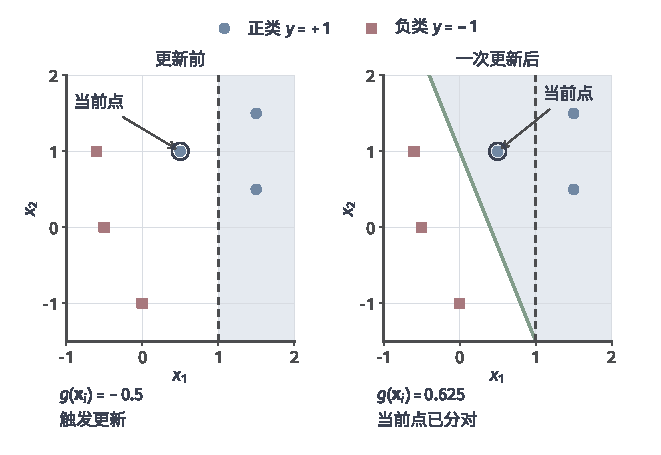
\includegraphics[width=112.000mm]{figures/04-classic-models/00-shared/matplotlib/classification-perceptron-update/figure.pdf}
  \caption{错分正类点触发的一次感知机更新。六个点为教学构造，坐标无量纲，两面板共用坐标范围；蓝圆、红方分别为正负类，黑色圆环标出当前点。浅蓝区域为正类预测区域，虚线为旧边界$x_1=1$，绿色实线为新边界$1.25x_1+0.5x_2=0.5$。偏置随权重一起更新，当前点由负得分变为正得分。}
  \label{fig:classification-perceptron-update}
\end{figure}

\begin{algorithm}[带遍历上限的感知机训练]
  \label{alg:classification-perceptron}
  \begin{algorithmic}[1]
    \Require $D_n$，固定学习率$\eta>0$，最大遍历轮数$E\geq1$
    \Ensure 参数$\tilde{\bm{w}}$与是否已验证收敛的状态
    \State $\tilde{\bm{w}}\gets\bm{0}$
    \For{$e=1,\ldots,E$}
      \State $m\gets0$
      \For{$i=1,\ldots,n$}
        \State $\tilde{\bm{x}}_i\gets(\bm{x}_i^{\top},1)^{\top}$
        \If{$y_i\langle\tilde{\bm{w}},\tilde{\bm{x}}_i\rangle\leq0$}
          \State $\tilde{\bm{w}}\gets\tilde{\bm{w}}+\eta y_i\tilde{\bm{x}}_i$
          \State $m\gets m+1$
        \EndIf
      \EndFor
      \If{$m=0$}
        \State \Return $(\tilde{\bm{w}},\text{已收敛})$
      \EndIf
    \EndFor
    \State \Return $(\tilde{\bm{w}},\text{达到轮数上限})$
  \end{algorithmic}
\end{algorithm}

一整轮没有更新时，所有样本都是在同一个参数下得到严格正的有符号得分，才构成收敛证据。达到轮数上限时返回的是预算内的当前解，可分性仍未由这一停止状态判定。稠密实现每轮需要$O(nd)$运算，除训练集外只需$O(d)$参数空间；样本访问顺序可以改变输出的分隔面。

从优化角度看，定义\term{感知机损失}（perceptron loss）
\begin{equation}
  \label{eq:classification-perceptron-loss}
  \ell_{\mathrm{P}}(\tilde{\bm{w}};\bm{x}_i,y_i)
    =\max\{0,-y_i\langle\tilde{\bm{w}},\tilde{\bm{x}}_i\rangle\}.
\end{equation}
为了把这项损失用于更新，先看它的两段：当带符号得分为负时，对参数求导得到$-y_i\tilde{\bm{x}}_i$；得分为正时，损失恒为零，梯度也是$\bm 0$。两段在零得分处相接，却给出不同斜率，普通梯度在这里没有定义。由于损失仍是凸的，可以使用次梯度；在交点处选择$-y_i\tilde{\bm{x}}_i$，仍满足支撑损失的仿射下界条件，也就得到式~\eqref{eq:classification-perceptron-update}。这一求解依据见\BookSectionRef{sec:opt-subgradient-methods}{第一卷“数学准备”的“基于次梯度的求解”节}。

上述更新逐样本执行；随机抽取样本时才相应成为随机次梯度下降。这里使用的是零间隔损失，不是标准的\term{合页损失}（hinge loss）$\max\{0,1-y_i\langle\tilde{\bm{w}},\tilde{\bm{x}}_i\rangle\}$。前者在零参数处就对所有样本取零，因此“感知机损失为零”本身不能证明分类正确；算法在零得分处仍更新的约定不可省略。

\subsubsection{理论分析}
\label{sec:classification-perceptron-analysis}

\paragraph{表达能力}
单层感知机的候选规则为$\operatorname{sign}(\bm w^\top\bm x+b)$。目标本来就是一个半空间时，这个候选类可以精确表示它；目标依赖特征交互时，则可能无法同时满足全部类别条件。

例如，取$(1,1)$、$(-1,-1)$、$(1,-1)$、$(-1,1)$四点作为输入域，同号坐标的目标标签为$-1$，异号坐标为$+1$。正、负两对点的中点都在原点。若一个仿射得分把四点全分对，正类得分的平均必须非负，负类得分的平均必须为负；两者却都等于$b$，产生矛盾。因此候选类中的每个函数至少在一个点上偏离目标。增加特征$x_1x_2$后，得分$-x_1x_2$恰好满足四点的目标标签，这才改变了候选空间的表示限制。

\paragraph{收敛性}
每次修正可能破坏已有判断，为什么这些修正不会无穷持续？关键是存在一个始终把所有样本分对的参考方向：更新朝该方向取得线性累积的进展，而参数范数的平方只能线性增长。Novikoff在1962年报告的证明清楚展示了这两个增长速度之间的矛盾\scite{novikoff1962}。

\begin{theorem}[感知机在有界可分样本下的最大更新次数]
  \label{thm:classification-perceptron-mistakes}
  若$D_n$满足式~\eqref{eq:classification-perceptron-margin}，从零参数出发，以固定$\eta>0$按式~\eqref{eq:classification-perceptron-update}更新，则对任意样本访问顺序，错误更新次数$M$满足
  \[
    M\leq\left(\frac R\gamma\right)^2 .
  \]
  这里错误更新包括零得分时的更新。若持续完整遍历训练集，且不因预算提前退出，算法在有限轮后得到所有训练样本上有符号得分均严格为正的参数。
\end{theorem}

\begin{proof}
  设第$t+1$次更新使用样本$i_t$。沿单位参考方向$\bm{u}^\ast$考察更新，得到
  \begin{align*}
    \langle\tilde{\bm{w}}^{(t+1)},\bm{u}^\ast\rangle
      &=\langle\tilde{\bm{w}}^{(t)},\bm{u}^\ast\rangle
        +\eta y_{i_t}\langle\tilde{\bm{x}}_{i_t},\bm{u}^\ast\rangle\\
      &\geq\langle\tilde{\bm{w}}^{(t)},\bm{u}^\ast\rangle+\eta\gamma .
  \end{align*}
  从零参数累加$M$次，便有
  \[
    \langle\tilde{\bm{w}}^{(M)},\bm{u}^\ast\rangle
      \geq M\eta\gamma .
  \]
  另一方面，展开更新后的平方范数：
  \begin{align*}
    \|\tilde{\bm{w}}^{(t+1)}\|_2^2
      &=\|\tilde{\bm{w}}^{(t)}\|_2^2
        +2\eta y_{i_t}
          \langle\tilde{\bm{w}}^{(t)},\tilde{\bm{x}}_{i_t}\rangle\\
      &\quad+\eta^2\|\tilde{\bm{x}}_{i_t}\|_2^2\\
      &\leq\|\tilde{\bm{w}}^{(t)}\|_2^2+\eta^2R^2 .
  \end{align*}
  不等式使用了更新条件：交叉项非正；并使用同一增广空间中的长度界$R$。再次累加，得到$\|\tilde{\bm{w}}^{(M)}\|_2^2\leq M\eta^2R^2$。由Cauchy--Schwarz不等式和$\|\bm{u}^\ast\|_2=1$，
  \[
    M\eta\gamma
      \leq\langle\tilde{\bm{w}}^{(M)},\bm{u}^\ast\rangle
      \leq\|\tilde{\bm{w}}^{(M)}\|_2
      \leq\eta R\sqrt{M}.
  \]
  $M=0$时结论直接成立；$M>0$时除以$\eta\sqrt M$再平方，得到所述界。因此更新不可能无限发生。持续完整遍历会在最后一次更新之后再检查所有样本；若仍有非正得分就还会更新，产生矛盾，故最终必有一整轮没有更新。
\end{proof}

这个界不显式含$n$，也不依赖访问顺序，但$R$和$\gamma$随数据而定；增加样本可能缩小可分间隔。它只约束更新次数，不包括寻找错误时检查正确样本的开销。对于算法~\ref{alg:classification-perceptron}的逐轮扫描，若不提前截断，至多需要$M+1$轮，包括最终的无更新确认轮。

若数据不可分，有限更新保证失效，持续遍历可能反复更新，此时可以限制训练预算并保留历史较好解，或采用允许间隔违约的在线方法。这些处理改变了停止或选解方式，仍须分别分析。

\paragraph{泛化性}
测试风险需要训练更新之外的统计条件。前述错误次数证明只考察给定样本的几何结构；若要判断未来预测，需要规定抽样分布与训练后返回哪个分类器。Cesa-Bianchi、Conconi与Gentile在2004年研究了这种联系：由独立同分布样本上的在线表现控制历史预测规则的风险，并讨论相应的输出选择方法\scite{cesabianchi2004generalization}。

下面给出一个期望风险的简单结论，说明额外条件怎样进入证明。按独立同分布的到达顺序，仅遍历$D_n$一次，从零参数出发使用固定学习率$\eta>0$和原更新规则。用$f_i$表示看到第$i$个样本之前的分类器；它只依赖$D_{i-1}$，其中$D_0$为空。这里$i$计数已访问的样本位置，与只计实际更新的$t$不同。训练后独立地从$\{1,\ldots,n\}$均匀抽取$I$，返回$f_I$，使输出规则与下述期望风险证明一致。

\begin{theorem}[感知机随机历史输出在可分分布下的期望风险界]
  \label{thm:classification-perceptron-risk}
  设训练样本独立同分布，测试样本独立来自同一分布。假设存在固定的单位向量$\bm{u}^\ast$及常数$R<\infty$、$\gamma>0$，使
  \[
    \|\tilde{\bm{x}}\|_2\leq R,\qquad
    y\langle\bm{u}^\ast,\tilde{\bm{x}}\rangle\geq\gamma
    \quad\text{几乎必然}.
  \]
  对上述单遍历训练和随机输出规则，有
  \begin{equation}
    \label{eq:classification-perceptron-risk}
    \mathbb{E}_{D_n,I}\!\left[R(f_I\mid D_n,I)\right]
      \leq\frac{R^2}{n\gamma^2}.
  \end{equation}
\end{theorem}

\begin{proof}
  令$e_i=\mathbb{1}\{f_i(\bm{x}_i)\ne y_i\}$。由于$f_i$尚未使用第$i$个样本，独立性给出
  \[
    \mathbb{E}[e_i\mid D_{i-1}]
      =R(f_i\mid D_{i-1}).
  \]
  对两边取期望，再对均匀的$I$平均，就有
  \[
    \mathbb{E}_{D_n,I}[R(f_I\mid D_n,I)]
      =\frac1n\sum_{i=1}^{n}\mathbb{E}[e_i].
  \]
  每次预测错误都会触发更新，零得分且预测正确时也可能更新，故$\sum_i e_i\leq M$。分布层面的共同间隔和长度界使定理~\ref{thm:classification-perceptron-mistakes}几乎必然适用于每个训练序列，于是$M\leq R^2/\gamma^2$，代入即得结论。
\end{proof}

这里的$R$和$\gamma$约束整个数据分布。式~\eqref{eq:classification-perceptron-risk}对训练抽样及随机历史状态取平均；当上界小于$1$时，它提供非平凡的期望风险控制。最终参数或多轮训练使用不同的输出与依赖关系，需各自分析：尤其在多轮中，当前样本已经参与既有参数的形成。不同的历史选解规则需要分别检查其训练依赖。

\subsubsection{优化表达能力}

若问题在于原空间不能线性分开，可把输入换成特征映射$\bm{\phi}(\bm{x})$。核函数$K(\bm{x},\bm{z})=\langle\bm{\phi}(\bm{x}),\bm{\phi}(\bm{z})\rangle$直接计算映射后的内积，省去显式构造高维坐标，得到\term{核感知机}（kernel perceptron）。为与前文偏置一致，使用增广映射$(\bm{\phi}(\bm{x}),1)$及其核$\tilde K(\bm{x},\bm{z})=K(\bm{x},\bm{z})+1$。零初始化、单位学习率下，参数在特征空间中是更新样本的线性组合，预测可写为
\begin{equation}
  \label{eq:classification-kernel-perceptron}
  f(\bm{x})=\operatorname{sign}
    \left(\sum_{i=1}^{n}\alpha_i y_i
      [K(\bm{x}_i,\bm{x})+1]\right).
\end{equation}
这里$\alpha_i$是样本$i$的更新次数；遇到非正有符号得分时令$\alpha_i\leftarrow\alpha_i+1$。必须选用正定核，即它在任意有限输入集上生成半正定Gram矩阵，才能作上述内积解释；有限更新还要求增广特征空间内存在正间隔，长度界相应变为$\sqrt{K(\bm{x}_i,\bm{x}_i)+1}$的上界。预测需要访问系数非零的样本，数量可能随训练增长。将内积推广到特征空间的思路可追溯至Aizerman、Braverman与Rozonoer在1964年的势函数研究\scite{aizerman1964}。

核与输入尺度共同决定映射后是否可分；预测成本则由需要保存的更新样本数决定。核化改变表示，不替代对标签噪声、停止规则和样本外误差的检查。

\subsubsection{优化泛化能力}

若希望减轻预测对最后一次参数更新的依赖，可以汇总训练过程中的多个状态。Freund与Schapire在1999年研究的\term{投票感知机}（voted perceptron）保存历次权重，并按各状态持续使用的次数加权投票；同一论文也比较了用历史得分平均代替投票的方式\scite{freund1999}。沿用本节的增广表示，设保存的状态为$\tilde{\bm w}_1,\ldots,\tilde{\bm w}_K$，$c_k>0$是第$k$个状态的计数，则投票预测为
\begin{equation}
  f_{\mathrm V}(\bm x)
  =\operatorname{sign}\!\left[
    \sum_{k=1}^{K}c_k\operatorname{sign}
       (\tilde{\bm w}_k^\top\tilde{\bm x})\right].
  \label{eq:classification-voted-perceptron}
\end{equation}
计数必须与更新同步。初始零参数的计数取零；本次检查未触发更新时，将当前状态的计数加一；触发更新时，保存新参数并把新状态的计数置为一，不再给被替换的旧状态加一。这里沿用非正有符号得分触发更新的约定，最后忽略计数为零的状态。计数取决于访问顺序与训练预算，并不是对新样本准确率的独立测量。保存与预测$K$个稠密状态均需考虑$O(Kd)$的代价。

\term{平均感知机}（averaged perceptron）改为先把这些增广参数平均：
\[
  \bar{\bm w}=\frac{\sum_{k=1}^{K}c_k\tilde{\bm w}_k}
                        {\sum_{k=1}^{K}c_k},
  \qquad
  f_{\mathrm A}(\bm x)=\operatorname{sign}
                    (\bar{\bm w}^\top\tilde{\bm x}).
\]
线性实现可在训练时累计参数和，最终只保存一组参数，额外存储与单次预测均为$O(d)$。投票先对每个得分取符号，再汇总标签；参数平均先汇总实值得分，再取符号，二者一般不同。前者的最终规则可以组合多个半空间判断，后者仍返回单个仿射得分；它们都改变训练结束后的输出方式，不能仅凭“汇总历史”判断哪种更适合任务。

\subsubsection{优化计算能力}

\paragraph{保存预算内的较优参数}
不可分数据可能使参数反复改变，预算结束时的权重未必是已经检查过的最好结果。\term{口袋算法}（Pocket algorithm）通过保存历史参数处理这个问题。常用版本额外保存$\tilde{\bm{w}}_{\mathrm{pocket}}$：每次检查候选参数时，计算全训练集零一错误数，仅在严格改进时替换记录；预算用尽后返回记录参数。它适用于噪声或矛盾标签数据，返回预算内已检查候选中的最小训练错误解；每次候选比较还需要评估全训练集。Gallant在1990年的论文中系统讨论了Pocket及相关学习方法\scite{gallant1990}。

Pocket只改变返回哪组历史参数，候选得分仍是原坐标中的仿射函数。它需要额外评估全部训练样本，也不能消除前面异或任务的表示限制。这里改善的是有限预算下的返回规则，并未使不可分数据上的原更新停止，也不保证找到所有仿射分类器中的最小训练错误解。

\paragraph{控制单步参数改动}
若希望每次更新不仅改正符号，还达到指定得分间隔，\term{被动攻击算法}（passive-aggressive algorithm, PA）把“尽量少改参数”和“满足当前样本的单位间隔”合成一个投影问题。用$\bm{v}$表示待求的新增广参数，
\begin{equation}
  \label{eq:classification-pa-projection}
  \begin{aligned}
    \min_{\bm{v}}\quad&
      \frac12\|\bm{v}-\tilde{\bm{w}}\|_2^2\\
    \text{满足}\quad&
      y_i\langle\bm{v},\tilde{\bm{x}}_i\rangle\geq1 .
  \end{aligned}
\end{equation}
令$\ell_i=\max\{0,1-y_i\langle\tilde{\bm{w}},\tilde{\bm{x}}_i\rangle\}$。约束已满足时参数不变；否则，拉格朗日驻点要求$\bm{v}=\tilde{\bm{w}}+\tau_i y_i\tilde{\bm{x}}_i$，将活跃约束代回即得
\[
  \tau_i=\frac{\ell_i}{\|\tilde{\bm{x}}_i\|_2^2},
  \qquad
  \tilde{\bm{w}}\leftarrow
    \tilde{\bm{w}}+\tau_i y_i\tilde{\bm{x}}_i .
\]
因此PA在间隔足够时“被动”，不足时按违约大小调整。增广方式也意味着这里把偏置变化纳入距离惩罚。噪声下硬性满足当前样本可能调整过大，PA-I可用$\tau_i=\min\{\lambda_{\mathrm{PA}},\ell_i/\|\tilde{\bm{x}}_i\|_2^2\}$限制步长，其中$\lambda_{\mathrm{PA}}>0$控制容忍程度。Crammer等人的2006年论文统一分析了这些在线大间隔方法；其保证针对在线更新的损失与间隔行为\scite{crammer2006}。
PA的单位间隔要求改变单步参数选择，候选得分仍是仿射函数。因此它与基本感知机、Pocket共享原坐标中的表示限制；间隔要求本身不能表达异或交互。

\subsubsection{支持多分类预测场景}

\label{sec:classification-perceptron-multiclass}

对$C$类问题，把标签改为$y_i\in\{1,\ldots,C\}$，每类维护一组增广参数$\tilde{\bm{w}}_c=(\bm{w}_c^{\top},b_c)^{\top}$，得分和预测为
\[
  s_c(\bm{x})=\langle\tilde{\bm{w}}_c,\tilde{\bm{x}}\rangle,
  \qquad
  \hat y=\argmax_{c\in\{1,\ldots,C\}}s_c(\bm{x}).
\]
平局仍按最小类别索引处理。这个构造把正确类别的得分与每个竞争类别作比较，也可用\term{Kesler构造}（Kesler construction）把这些比较写成一个扩展空间中的线性可分问题。

第$c$类获胜要求$s_c(\bm x)\geq s_j(\bm x)$对每个竞争类成立，平局处再按既定顺序处理。因此每类区域是若干半空间的交，仍是凸区域。它可以表示多类线性分区，却不能在原坐标中把某一类分成被其他类别隔开的多个区域；这种任务需要新的特征或不同的输出表示。

遇到$\hat y_i\ne y_i$时，只提高正确类别的参数并降低错误获胜类别的参数：
\begin{equation}
  \label{eq:classification-perceptron-multiclass-update}
  \begin{aligned}
    \tilde{\bm{w}}_{y_i}
      &\leftarrow\tilde{\bm{w}}_{y_i}+\eta\tilde{\bm{x}}_i,\\
    \tilde{\bm{w}}_{\hat y_i}
      &\leftarrow\tilde{\bm{w}}_{\hat y_i}-\eta\tilde{\bm{x}}_i .
  \end{aligned}
\end{equation}
其余类别不变，两个类别的偏置也随各自最后一个分量同时更新。若平局后预测错误，同样更新；若已选择正确类别，则该规则不更新。与二分类中所有零得分均更新的约定不同，这里直接按最终预测是否正确判断。

收敛条件也必须改为多类的得分差条件。把各类参数按行堆成$\tilde{\bm{W}}\in\mathbb{R}^{C\times(d+1)}$；假设存在$\|\bm{U}^\ast\|_{\mathrm{F}}=1$和$\gamma_{\mathrm{mc}}>0$，使对所有$i$和$c\ne y_i$都有
\[
  \langle\bm{U}_{y_i,:}^\ast-\bm{U}_{c,:}^\ast,
    \tilde{\bm{x}}_i\rangle\geq\gamma_{\mathrm{mc}} .
\]
这里$\|\cdot\|_{\mathrm{F}}$是所有矩阵元素平方和的平方根，行向量的内积按对应坐标计算。一次更新的方向矩阵仅两行非零，分别为$\tilde{\bm{x}}_i^{\top}$与$-\tilde{\bm{x}}_i^{\top}$，其平方范数至多为$2R^2$。它与$\bm{U}^\ast$的内积至少为$\gamma_{\mathrm{mc}}$；与当前参数的内积则为$s_{y_i}(\bm{x}_i)-s_{\hat y_i}(\bm{x}_i)\leq0$。因此零初始化时完全沿用二分类证明，得到
\[
  M\eta\gamma_{\mathrm{mc}}
    \leq\|\tilde{\bm{W}}^{(M)}\|_{\mathrm{F}}
    \leq\eta R\sqrt{2M},
  \qquad
  M\leq\frac{2R^2}{\gamma_{\mathrm{mc}}^2}.
\]
有限更新保证因而保留下来，但它要求所有正确类与竞争类之间都具有共同的正间隔，而不是只检查任意一对类别。

\subsubsection{支持结构化输出预测场景}

如果任务是给一句话中的每个词标注词性，输出就从一个类别变成了一整条标签序列。逐词独立判类无法在同一个得分中评价相邻标签的组合；我们希望同时比较不同候选序列，并在预测错误时调整整条序列用到的特征。\term{结构化感知机}（structured perceptron）把多分类的得分比较推广到结构之间，用联合特征$\bm{\phi}(\bm{x},y)$描述输入与候选结构，预测
\[
  \hat y_i=\argmax_{y\in Y(\bm{x}_i)}
    \langle\bm{\theta},\bm{\phi}(\bm{x}_i,y)\rangle ,
\]
其中$Y(\bm{x}_i)$是候选结构集合，$\bm{\theta}$是与联合特征同维的参数。解码错误时进行
\[
  \bm{\theta}\leftarrow\bm{\theta}
    +\eta\bigl[\bm{\phi}(\bm{x}_i,y_i)
      -\bm{\phi}(\bm{x}_i,\hat y_i)\bigr].
\]
联合特征决定哪些结构差异能够进入比较。若同一输入上的两个候选结构具有完全相同的$\bm\phi(\bm x,y)$，它们对所有参数都同分，候选得分无法区分两者，只能由固定的平局规则选择其中一个。词性标注中的相邻标签关系或更远处的依赖，因而需要由相应的特征记录；解码搜索再精确，也不能恢复特征没有保留的差异。

需要的类别或结构偏置也作为联合特征中的相应指示分量处理；对所有候选都相同的常数项会在得分差中消去。结构化输出增加了解码成本，近似解码还可能改变哪些样本触发更新，需要与特征设计一同评价。Collins在2002年将这种更新与参数平均用于序列标注，提供了词性标注和短语识别等实例，也为比较感知机与条件随机场等结构化模型提供了参照\scite{collins2002}。

\subsubsection{小结}
\label{sec:classification-perceptron-summary}

感知机用当前样本的标签直接修正边界，免去了先拟合类分布的步骤。一次更新提高当前样本的有符号得分，却可能改变其他样本的判断；因此样本顺序、停止预算和返回规则都属于实际学习过程。它提供简洁的增量训练方式，原坐标中的单个边界仍受仿射表示限制。

预算结束时怎样利用历史参数，是不可分或尚未收敛数据上的一个具体问题。Gallant讨论的Pocket保存已检查的较好状态，代价是重复评估训练集；Freund与Schapire的投票感知机让多个状态共同判类，代价是状态存储与多次预测。平均感知机把历史压缩成一组参数，减轻线性预测的负担，但它与标签投票采用不同的汇总规则。选择时需要比较同一访问顺序与预算下的分类误差和存储成本。

若缺的是非线性输入关系，核感知机把内积换到特征空间，预测则需要保留更新样本。PA处理的困难不同：当一步更新还不足以达到所需间隔时，Crammer等用最小参数改动满足当前约束，噪声下再限制过大的调整。它改变单步目标，原坐标中的表示仍然线性。

序列标注等结构化任务又需要改变输出比较。Collins的结构化感知机通过联合特征评价完整序列，解码成本随候选结构增加。输入表示、单步目标与输出结构解决不同困难，不能用增加遍历次数代替这些改变。

\subsection{支持向量机（SVM）}
\label{sec:classification-svm}

感知机回答了一个基本问题：如果训练样本能够被某个超平面分开，怎样通过错误驱动的更新找到一个分离器？但分开训练样本并不意味着分界的位置已经合适。同一批可分数据往往允许许多分离超平面，即使从零参数开始，感知机的结果仍会受样本顺序和更新规则影响。一个紧贴训练样本的边界虽然没有训练错误，却可能在输入受到很小扰动时改变预测。要在这些分离器之间作出选择，还需要说明什么样的边界更值得保留。

\term{支持向量机}（support vector machine，SVM）以训练样本到边界的距离选择分隔面：在正确分离样本的前提下，增大最近样本到边界的距离，称为最大间隔。给定特征表示与距离度量后，这个几何准则使边界具有可比较的尺度。不可分数据可以通过松弛约束处理，非线性关系则可以通过改变特征表示处理；两种扩展分别作用于误差容忍与候选函数。

核与松弛约束解决不同困难：Boser、Guyon与Vapnik在1992年把最大间隔训练与核表示结合，Cortes与Vapnik在1995年进一步系统发展了容许间隔违反的形式。前者改变非线性特征的使用方式，后者让噪声或类别重叠进入带惩罚的训练目标\scite{boser1992margin,cortes1995}。下面先从可分数据推导间隔目标与对偶，再用SMO说明参数怎样求出，最后分别改变输入表示、误差容忍和类别竞争。

\subsubsection{模型结构}
\label{sec:classification-svm-model}

沿用二分类标签约定，设训练集为$D_n=\{(\bm{x}_i,y_i)\}_{i=1}^n$，其中$\bm{x}_i\in\mathbb{R}^d$、$y_i\in\{-1,+1\}$，并假设两类均非空。令实值得分为$g(\bm{x})=\bm{w}^{\top}\bm{x}+b$，其中$\bm{w}\in\mathbb{R}^d$、$b\in\mathbb{R}$且$\bm{w}\ne\bm{0}$。决策超平面是$g(\bm{x})=0$，预测规则为$\hat y(\bm{x})=\operatorname{sign}(g(\bm{x}))$；若得分恰为零，约定预测为$+1$。

仅比较$y_i g(\bm{x}_i)$还不能比较不同超平面。把$(\bm{w},b)$同时乘以任意正数，分类结果不变，这个数值却会随之放大：同一条直线，把权重都乘以$100$，每个样本的得分也乘以$100$，直线却毫无变化。因此得分本身的“大小”带有任意性，不能直接当作距离或安全裕度。为区分参数尺度与真实距离，定义样本的\term{函数间隔}（functional margin）为$m_i=y_i g(\bm{x}_i)$，定义其\term{几何间隔}（geometric margin）为
\begin{equation}
  \gamma_i
  =\frac{y_i(\bm{w}^{\top}\bm{x}_i+b)}
         {\lVert\bm{w}\rVert_2},
  \qquad
  \gamma=\min_{1\le i\le n}\gamma_i.
  \label{eq:classification-svm-margin}
\end{equation}
函数间隔保留了得分的尺度；几何间隔除以法向量长度，得到沿法向方向测量的有符号距离。乘上真实标签后的得分满足$y_i g(\bm x_i)>0$时，样本位于正确类别一侧，这个距离为正。$g(\bm x_i)=0$时，样本就在决策边界上：正类虽然按平局规则被判对，几何间隔仍为零，因而没有正半径的扰动容忍保证。若输入改变为$\bm{x}_i+\bm{\Delta}$，由Cauchy--Schwarz不等式可得
\[
  y_i g(\bm{x}_i+\bm{\Delta})
  \ge y_i g(\bm{x}_i)
      -\lVert\bm{w}\rVert_2\lVert\bm{\Delta}\rVert_2.
\]
因此，$\lVert\bm{\Delta}\rVert_2<\gamma_i$时预测不会翻转。这说明间隔量化当前特征空间中、由该范数限定的输入扰动容忍程度；分布变化需要另外规定变化方式。

严格线性可分意味着存在$(\bm{w},b)$使所有$m_i>0$。由于样本数有限，可以将这组参数除以$\min_i m_i$，得到$\min_i m_i=1$的规范化表示。在该表示下，最近样本到决策超平面的单侧距离为$1/\lVert\bm{w}\rVert_2$；两个平行超平面$g(\bm{x})=+1$与$g(\bm{x})=-1$之间的总宽度则是$2/\lVert\bm{w}\rVert_2$。本节将前者记为$\gamma$，不把单侧间隔与两侧带宽混用。

最大化$\gamma$于是等价于最小化$\lVert\bm{w}\rVert_2$。平方与正比例因子不改变最优解，却使求导更方便，得到\term{硬间隔}（hard margin）SVM的原始问题：
\begin{equation}
  \begin{aligned}
    \min_{\bm{w},b}\quad&
      \frac12\lVert\bm{w}\rVert_2^2\\
    \text{s.t.}\quad&
      y_i(\bm{w}^{\top}\bm{x}_i+b)\ge1,
      \quad i=1,\ldots,n.
  \end{aligned}
  \label{eq:classification-svm-hard-primal}
\end{equation}
这里的“硬”表示每个样本都必须满足间隔约束，不能用其他样本的改善来补偿某个样本的违反。约束写为大于等于$1$并没有放弃规范化：若一个可行解的最小函数间隔严格大于$1$，将参数一起缩小就能降低目标，所以最优解必有紧约束。

可分时这个规范化问题有唯一解。先用一维点集观察间隔怎样选择边界，再推导求解所需的最优性条件。

\begin{example}[单侧间隔与带宽]
  \label{ex:classification-svm-one-dimensional}
  考虑一维教学数据$(x_1,y_1)=(-1,-1)$、$(x_2,y_2)=(1,+1)$、$(x_3,y_3)=(-2,-1)$和$(x_4,y_4)=(2,+1)$。任意落在$-1$与$1$之间的阈值都能正确分类，但只有阈值$0$使两侧最近距离的较小者达到最大。规范化最优解为$w^{\ast}=1$、$b^{\ast}=0$；最近样本的单侧距离为$1$，两条支持超平面在此退化为两个点$-1$与$1$，其间距离为$2$。更远的两个样本不限制这一最优间隔。
\end{example}

\subsubsection{参数学习}
\label{sec:classification-svm-learning}

每个间隔约束对最优边界的影响，可由对应的拉格朗日乘子表示。这里先用一句话说明“对偶”到底在做什么：原问题是在“选一条直线”，让它离样本尽量远；对偶则换一个视角，改问“每个训练样本对这条直线有多大约束力”。每个样本分到一个非负权重$\alpha_i$，离边界远、不构成约束的样本权重为零，真正“撑住”边界两侧的少数样本权重为正，它们就是后面的支持向量。\term{对偶问题}（dual problem）把这些约束权重作为优化变量，既揭示参与预测的样本，也把训练表示为样本间内积运算，为核化提供入口。原始与对偶的变量数分别受特征维数和样本数影响，计算选择还要结合求解器与数据稀疏性。

将约束写为$1-y_i(\bm{w}^{\top}\bm{x}_i+b)\le0$，引入$\alpha_i\ge0$，记$\bm{\alpha}=(\alpha_1,\ldots,\alpha_n)^{\top}$。拉格朗日函数为
\begin{equation}
  \begin{aligned}
    L(\bm{w},b,\bm{\alpha})
    ={}&\frac12\lVert\bm{w}\rVert_2^2\\
      &+\sum_{i=1}^n\alpha_i
        \bigl[1-y_i(\bm{w}^{\top}\bm{x}_i+b)\bigr].
  \end{aligned}
  \label{eq:classification-svm-hard-lagrangian}
\end{equation}
对一个可行$(\bm{w},b)$，$\sup_{\bm{\alpha}\ge\bm{0}}L$等于原始目标；若有约束违反，对应乘子趋于无穷会使上确界为正无穷。因此原始最优值可写为$\inf_{\bm{w},b}\sup_{\bm{\alpha}\ge\bm{0}}L$。反过来，先对$(\bm{w},b)$取下确界再最大化，得到原始最优值的下界。强对偶条件决定两种次序何时给出相同值。

这里可以直接核验\term{Slater条件}（Slater's condition）：它要求存在严格满足不等式约束的点。取一个严格分离器，并把参数放大到所有函数间隔都严格大于$1$，就得到所需点。结合目标凸、约束仿射以及定理\ref{thm:classification-svm-hard-unique}证明的最优值可达性，可得强对偶与最优乘子的存在性。

现在计算$q(\bm{\alpha})=\inf_{\bm{w},b}L(\bm{w},b,\bm{\alpha})$。由于$b$没有二次项，若$\sum_i\alpha_i y_i\ne0$，沿$b$的某个方向就有$L\to-\infty$。要使$q$有限，必须满足等式约束；关于$\bm{w}$的极小值则由驻点给出：
\begin{equation}
  \bm{w}=\sum_{i=1}^n\alpha_i y_i\bm{x}_i,
  \qquad
  \sum_{i=1}^n\alpha_i y_i=0.
  \label{eq:classification-svm-stationarity}
\end{equation}
令$\bm{v}=\sum_i\alpha_i y_i\bm{x}_i$，代入后涉及权重的两项变为$\frac12\lVert\bm{v}\rVert_2^2-\lVert\bm{v}\rVert_2^2$，而$b$项为零。展开$\lVert\bm{v}\rVert_2^2$，便得到
\begin{equation}
  \begin{aligned}
    \max_{\bm{\alpha}}\quad&
      q(\bm{\alpha})
      =\sum_{i=1}^n\alpha_i
       -\frac12\sum_{i,j=1}^n
          \alpha_i\alpha_j y_i y_j
          \bm{x}_i^{\top}\bm{x}_j\\
    \text{s.t.}\quad&
      \sum_{i=1}^n\alpha_i y_i=0,\qquad
      \alpha_i\ge0,\quad i=1,\ldots,n.
  \end{aligned}
  \label{eq:classification-svm-hard-dual}
\end{equation}
二次项矩阵的元素为$\bm{Q}_{i,j}=y_i y_j\bm{x}_i^{\top}\bm{x}_j$。对任意$\bm{a}\in\mathbb{R}^n$，有$\bm{a}^{\top}\bm{Q}\bm{a}=\lVert\sum_i a_i y_i\bm{x}_i\rVert_2^2\ge0$，所以$q$是凹函数；它未必严格凹，因而对偶乘子未必唯一。

原始解与对偶解的联系可以用\term{Karush--Kuhn--Tucker条件}（Karush--Kuhn--Tucker conditions，KKT条件）完整表达。它们同时检查解是否满足约束、是否达到驻点，以及一个约束是否真的限制了目标的继续改善。在当前凸问题与Slater条件下，这组条件对最优性既必要又充分：
\begin{equation}
  \begin{aligned}
    &m_i^{\ast}=y_i g^{\ast}(\bm{x}_i)\ge1,
      \qquad \alpha_i^{\ast}\ge0,\\
    &\alpha_i^{\ast}(m_i^{\ast}-1)=0,
      \qquad i=1,\ldots,n,\\
    &\bm{w}^{\ast}
      =\sum_{i=1}^n\alpha_i^{\ast}y_i\bm{x}_i,
      \qquad \sum_{i=1}^n\alpha_i^{\ast}y_i=0.
  \end{aligned}
  \label{eq:classification-svm-hard-kkt}
\end{equation}
其中第三个关系是\term{互补松弛}（complementary slackness）：乘子与约束的剩余量不能同时为正。最后一行是关于权重与偏置的驻点条件。

把$\alpha_i^{\ast}>0$的样本称为\term{支持向量}（support vector），并记其索引集为$S=\{i:\alpha_i^{\ast}>0\}$。互补松弛说明，支持向量一定满足$m_i^{\ast}=1$，而$m_i^{\ast}>1$必有$\alpha_i^{\ast}=0$。反向推断却不成立：落在边界上的样本也可能具有零乘子。例如把示例\ref{ex:classification-svm-one-dimensional}中的$x_2=1$重复一次，正类边界点的乘子总和仍可为$1/2$，但这个总量可以全部分配给其中一个副本。超平面没有改变，对偶表示与支持向量索引集却可能改变。

求得$\bm{\alpha}^{\ast}$后，恢复模型只需
\begin{equation}
  \begin{aligned}
    \bm{w}^{\ast}
      &=\sum_{i\in S}\alpha_i^{\ast}y_i\bm{x}_i,\\
    b^{\ast}
      &=y_k-(\bm{w}^{\ast})^{\top}\bm{x}_k,
        \qquad k\in S.
  \end{aligned}
  \label{eq:classification-svm-recover}
\end{equation}
精确最优解下，任意支持向量都会给出同一偏置；数值计算中可以平均多个合适样本给出的估计。只有非零乘子进入预测，这就是SVM的稀疏表示。表示的实际大小取决于支持向量数，某些训练集的大部分乃至全部样本都可能具有非零乘子。

\paragraph{SMO 算法}
\label{sec:classification-svm-smo}

对偶把未知量换成了$n$个乘子，也带来了新的计算负担。若存储完整内积矩阵，需要$O(n^2)$空间；通用稠密求解中的一次矩阵分解就可能需要$O(n^3)$运算，具体总成本还取决于求解器与迭代次数。为了避开每轮求解大规模二次规划，Platt提出了\term{序列最小优化}（sequential minimal optimization，SMO）：每次只优化一个最小的可动变量组，把整个问题分解为可解析处理的二维子问题\scite{platt1998smo}。

一次至少需要调整两个乘子，因为$\sum_i\alpha_i y_i=0$且$y_i\ne0$，单独改变一个$\alpha_i$会破坏等式约束。选择两个不同索引$i,j$，固定其余乘子，记更新前数值为$\alpha_i^{(t)},\alpha_j^{(t)}$，并令$s=y_i y_j\in\{-1,+1\}$。如果把新的$\alpha_j$写为$u$，等式约束要求
\begin{equation}
  \alpha_i(u)
  =\alpha_i^{(t)}
    +s\bigl(\alpha_j^{(t)}-u\bigr).
  \label{eq:classification-svm-smo-coupling}
\end{equation}
这样二维问题实际上只剩一个自由变量。对硬间隔，要求$u\ge0$且$\alpha_i(u)\ge0$，可行区间$[L,H]$为
\begin{equation}
  \begin{aligned}
    s=+1:\quad&
      L=0,\qquad H=\alpha_i^{(t)}+\alpha_j^{(t)},\\
    s=-1:\quad&
      L=\max\{0,\alpha_j^{(t)}-\alpha_i^{(t)}\},
      \qquad H=+\infty.
  \end{aligned}
  \label{eq:classification-svm-smo-hard-interval}
\end{equation}
同号时两乘子之和固定，因而有有限上界；异号时差固定，二者可以同时增大。这两种区间的差别来自标签符号对等式约束的影响。

为求沿这个区间的最优点，定义$\bm{K}_{i,j}=\bm{x}_i^{\top}\bm{x}_j$，并使用当前实值得分计算误差缓存
\[
  E_k=g^{(t)}(\bm{x}_k)-y_k,\qquad
  g^{(t)}(\bm{x})
  =\sum_{\ell=1}^n\alpha_\ell^{(t)}
     y_\ell\bm{x}_\ell^{\top}\bm{x}+b^{(t)}.
\]
$E_k$保留实值得分相对于标签的偏差，因而包含更新所需的距离信息；经过$\operatorname{sign}$得到的离散预测标签不再包含这部分信息。令$\Delta=u-\alpha_j^{(t)}$。由于$\Delta\alpha_i=-s\Delta$，权重变化为$y_j\Delta(\bm{x}_j-\bm{x}_i)$，代入$q$可以逐项得到
\begin{equation}
  \begin{aligned}
    q(u)-q(\alpha_j^{(t)})
      &=y_j(E_i-E_j)\Delta-\frac12\eta\Delta^2,\\
    \eta
      &=\bm{K}_{i,i}+\bm{K}_{j,j}-2\bm{K}_{i,j}\\
      &=\lVert\bm{x}_i-\bm{x}_j\rVert_2^2\ge0.
  \end{aligned}
  \label{eq:classification-svm-smo-gain}
\end{equation}
这里$q(u)$表示其余乘子固定、$\alpha_i$按式\eqref{eq:classification-svm-smo-coupling}联动后的目标。偏置不出现在对偶目标中；误差差$E_i-E_j$中的$b^{(t)}$也恰好相消。

当$\eta>0$时，一元凹二次函数的无约束最优点与区间最优点分别为
\begin{equation}
  \begin{aligned}
    u_{\mathrm{unc}}
      &=\alpha_j^{(t)}+\frac{y_j(E_i-E_j)}{\eta},\\
    \alpha_j^{(t+1)}
      &=\min\{H,\max\{L,u_{\mathrm{unc}}\}\},\\
    \alpha_i^{(t+1)}
      &=\alpha_i^{(t)}
        +s\bigl(\alpha_j^{(t)}-\alpha_j^{(t+1)}\bigr).
  \end{aligned}
  \label{eq:classification-svm-smo-update}
\end{equation}
剪裁只对一个自由变量进行，再由等式回代另一个；独立剪裁两个乘子会破坏耦合约束。若$L=H$，该变量对没有可行移动，应另选工作集。

$\eta=0$时，式\eqref{eq:classification-svm-smo-gain}变为线性函数，在有限区间上比较两个端点的目标即可；若目标恒定，保留旧值避免无效移动。严格可分的线性硬间隔问题中，$\eta=0$意味着两输入重合，它们不可能异号；同号重复点的目标沿可行线恒定。若出现零曲率、无穷上界且目标沿该方向无限增加，则应检查可分性假设、核矩阵与数值误差，并停止该次更新。

乘子更新以后还要调整偏置。记$\Delta\alpha_i=\alpha_i^{(t+1)}-\alpha_i^{(t)}$，$\Delta\alpha_j$同理。分别要求更新后的第$i$或第$j$个样本具有函数间隔$1$，解得
\begin{equation}
  \begin{aligned}
    b_i={}&b^{(t)}-E_i
       -y_i\Delta\alpha_i\bm{K}_{i,i}
       -y_j\Delta\alpha_j\bm{K}_{i,j},\\
    b_j={}&b^{(t)}-E_j
       -y_i\Delta\alpha_i\bm{K}_{i,j}
       -y_j\Delta\alpha_j\bm{K}_{j,j}.
  \end{aligned}
  \label{eq:classification-svm-smo-bias}
\end{equation}
硬间隔中，若更新后的$\alpha_i>0$，使用$b_i$；否则若$\alpha_j>0$，使用$b_j$。二者都为正且子问题精确求解时，这两个值一致；若都不能用于确定偏置，可暂取$(b_i+b_j)/2$。这一步利用当前工作集的条件更新偏置，其他样本是否满足KKT仍由后续全局扫描检查。

令$\Delta b=b^{(t+1)}-b^{(t)}$，其他样本的缓存可由
\[
  E_k^{(t+1)}
  =E_k^{(t)}
   +y_i\Delta\alpha_i\bm{K}_{i,k}
   +y_j\Delta\alpha_j\bm{K}_{j,k}
   +\Delta b
\]
更新，不必重新计算整个预测和。在示例\ref{ex:classification-svm-one-dimensional}中，从$\bm{\alpha}^{(0)}=\bm{0}$、$b^{(0)}=0$开始，选择$x_1=-1$与$x_2=1$，有$E_1=1$、$E_2=-1$、$\eta=4$，于是得到$\alpha_1=\alpha_2=1/2$和$b=0$。此时$w=1$，其余两个样本已经在间隔外；这一教学例子的最优解恰好由一次工作集更新达到；一般训练的迭代次数由后续选点与KKT误差决定。

\begin{algorithm}[硬间隔SMO的训练框架]
  \label{alg:classification-svm-smo}
  \begin{algorithmic}[1]
    \Require 两类非空且严格可分的$D_n$，容差$\varepsilon_{\mathrm{opt}}>0$，迭代上限$t_{\max}$
    \Ensure 可行乘子、偏置及停止状态
    \State 初始化$\bm{\alpha}^{(0)}=\bm{0}$、$b^{(0)}=0$、$E_k=-y_k$
    \For{$t=0,\ldots,t_{\max}-1$}
      \State 扫描KKT残差；若全部低于容差，返回“容差满足”
      \State 选取违反KKT的索引$i$，再选有可行改进的$j$
      \State 按式\eqref{eq:classification-svm-smo-hard-interval}计算$L,H$
      \State 求解一元子问题；退化时比较端点或更换变量对
      \State 联动更新两个乘子，更新$b$与误差缓存
    \EndFor
    \State 返回当前参数及“达到迭代上限，尚未认证收敛”
  \end{algorithmic}
\end{algorithm}

对于硬间隔，$\alpha_i=0$时应检查$m_i\ge1$，$\alpha_i>0$时应检查$m_i=1$，实际实现还要给“零乘子”设置数值容差。第二个变量可以优先选择误差差较大或预测目标增益较大的样本，并通过回退扫描持续检查其余违反条件的变量。算法\ref{alg:classification-svm-smo}给出共同框架，具体选点规则仍须保证持续处理违反KKT的变量。

SMO避免每轮分解整个稠密二次规划矩阵，但核缓存与工作集扫描仍有成本。

在线性问题中，也可以直接维护$\bm{w}$，不必先存储全部样本内积。软间隔形式还要处理合页损失：带符号得分跨过$1$时，损失从线性下降转为恒零，交点处没有普通梯度。次梯度方法允许在这个交点选择一个满足凸下界条件的方向，因而能继续更新参数。也可以按相应目标选择坐标下降算法。LIBLINEAR面向大规模稀疏线性分类提供了专门求解路线\scite{fan2008liblinear}。

\paragraph{最优解与停止证据}
\label{sec:classification-svm-analysis}
\label{sec:classification-svm-convergence}
\begin{theorem}[可分硬间隔问题的最优解]
  \label{thm:classification-svm-hard-unique}
  有限训练集严格线性可分、且两类均非空时，式\eqref{eq:classification-svm-hard-primal}存在唯一的规范化最优参数$(\bm w^\ast,b^\ast)$。
\end{theorem}
\begin{proof}
取一个可行解并限制目标不超过其值，权重便有界；一正一负两个样本的约束又给出偏置的上下界。因此可在非空紧水平集上取得最优值。平方范数对权重严格凸，所以不同最优解不能具有不同权重。

固定最优权重后，记正类投影最小值为$a_+$、负类投影最大值为$a_-$。可行偏置区间为$[1-a_+,-1-a_-]$，故$a_+-a_-\geq2$。若严格大于2，将权重和中心化偏置一起缩放到投影间距等于2，可保留全部约束却减小范数，违背最优性。故间距恰为2，偏置区间只剩一个点。
\end{proof}

SMO精确求解一个工作集时不会降低对偶目标，但目标单调不等于有限次到达全局最优。还要持续检查并处理所有违反KKT的变量，不能反复选择无法移动的变量对。实际训练以KKT容差给出近似最优证据；迭代预算先耗尽时，应保留“尚未达到容差”的状态。具体工作集规则及其收敛条件可参考分解算法研究\scite{osuna1997training,keerthi2002convergence,fan2005working}。

最大间隔是在固定表示和距离尺度下选择边界，不能单独保证新样本错误更少。线性SVM仍只能表示仿射分界；软化约束不会给它加入异或所需的交互特征。特征尺度、核与惩罚需要在训练集内部选择，最终用独立数据评价。下面把这几种改变分别写进得分和训练目标。

\subsubsection{核SVM与软间隔}

\paragraph{表示非线性分界}

\label{sec:classification-svm-kernels}

原坐标中的仿射得分只能给出直线或超平面边界。例如第\ref{sec:classic-overview-kernel-trick}节的圆内、圆外分类，需要曲线边界；调整原坐标中的线性系数，并不能让边界变成这条圆。核化改为在特征空间中学习线性得分，让原输入空间中的边界可以是非线性的。

SVM的对偶已经只含训练样本内积，所以可以用正定核$K$替换这些内积，在不显式构造高维坐标的情况下训练和预测。核技巧与合法性的理由见第\ref{sec:classic-overview-kernel-trick}节，常用核见第\ref{sec:classic-overview-common-kernels}节；这里将它们代入SVM的目标，推导相应的对偶与预测规则。

将$\bm{w}\in\mathbb{R}^d$换成$\bm{w}\in\mathcal{H}$，将平方范数换成$\lVert\bm{w}\rVert_{\mathcal{H}}^2$，硬间隔的内积推导便可在特征空间中进行。更具体地，把任意$\bm{w}$分解为训练特征张成空间内的部分与其正交部分，后者不改变任何训练得分，却只会增加范数。因此最优权重可以限制在有限个训练特征的张成空间中；驻点条件进一步给出$\bm{w}^{\ast}=\sum_i\alpha_i^{\ast}y_i\bm{\phi}(\bm{x}_i)$。若还允许样本违反单位间隔，并以$\lambda_{\mathrm s}>0$惩罚每单位违反量，对偶乘子便增加同一数值的上界；这一软间隔构造在下文展开。把硬间隔与这种允许违反的版本合写，核化对偶为
\begin{equation}
  \begin{aligned}
    \max_{\bm{\alpha}}\quad&
      \sum_{i=1}^n\alpha_i
       -\frac12\sum_{i,j=1}^n
          \alpha_i\alpha_j y_i y_j
          K(\bm{x}_i,\bm{x}_j)\\
    \text{s.t.}\quad&
      \sum_{i=1}^n\alpha_i y_i=0,\\
    &0\le\alpha_i\le\lambda_{\mathrm{s}},
      \qquad i=1,\ldots,n.
  \end{aligned}
  \label{eq:classification-svm-kernel-dual}
\end{equation}
在映射后严格可分的硬间隔情形，去掉乘子上界即可。新输入的得分与预测为
\begin{equation}
  \begin{aligned}
    g^{\ast}(\bm{x})
      &=\sum_{i\in S}\alpha_i^{\ast}y_i
         K(\bm{x}_i,\bm{x})+b^{\ast},\\
    \hat y(\bm{x})&=\operatorname{sign}(g^{\ast}(\bm{x})).
  \end{aligned}
  \label{eq:classification-svm-kernel-prediction}
\end{equation}
边界在$\mathcal{H}$中仍然是线性的，在原输入空间中则可能是曲线或曲面。SMO也只需把$\bm{K}_{i,j}$换成$K(\bm{x}_i,\bm{x}_j)$；此时$\eta=\lVert\bm{\phi}(\bm{x}_i)-\bm{\phi}(\bm{x}_j)\rVert_{\mathcal{H}}^2\ge0$，前面的区间、零曲率处理与偏置更新都继续适用。

不同核能表达的关系并不相同。二次多项式核$K(\bm x,\bm z)=(1+\bm x^\top\bm z)^2$的特征包含$x_1x_2$，所以候选得分$x_1+x_2-2x_1x_2-1/2$能精确区分前面的四点异或关系：两个负类点得分为$-1/2$，两个正类点得分为$1/2$。对RBF核$K(\bm x,\bm z)=\exp[-\|\bm x-\bm z\|_2^2/(2\sigma^2)]$，其中$\sigma>0$，候选得分$K(\bm0,\bm x)-t$在$0<t<1$时形成半径$\sigma\sqrt{-2\log t}$的球形正类区域。这里使用了一个核基函数与偏置，直接展示了直线表示缺少的半径关系。

这些例子只证明相应目标在候选得分族中，不保证训练必然找到它们。固定$p$次多项式核在一维仍只产生至多$p$次的多项式得分，非零得分至多有$p$个实根，因而不能表示任意多次交替的类别区间。范数、偏置和核尺度的限制又会约束可用得分及间隔；“使用核”本身不是对任意目标的逼近保证。

核技巧去掉了对显式特征维数的直接依赖，但没有去掉对样本量的依赖。构建完整Gram矩阵需要$O(n^2)$次核调用，之后还要执行优化迭代；两者合起来才是训练成本。若一次核计算耗时$t_K$，单次预测的主要核计算量是$O(|S|t_K)$。因此，无限维特征可以通过有限次内积运算使用，与“训练成本只由核计算决定”是两回事。

\paragraph{拟合无法完全分开的样本}
\label{sec:classification-svm-soft-margin}

硬间隔要求每个观测都能被严格分开。只要两个相同输入带有相反标签，约束就无解；即使仍然可分，一个位置异常的样本也可能把边界推向不适合大多数数据的位置。解决办法是允许样本违反间隔要求，但把违反量计入目标。这就是\term{软间隔}（soft margin）：间隔仍是选择边界的依据，却不再是每个观测都必须满足的硬性条件。

这里扩展的是允许拟合的数据条件：由必须满足全部硬间隔，改为允许带代价的间隔违反。固定输入表示时，候选得分仍是同一组仿射函数；软间隔不会把直线变成曲线，也不能消除相同输入带相反标签时的冲突。它使不可分样本上的目标仍可求解，而非保证比一个已有分类器具有更低的训练错误\scite{cortes1995}。

为第$i$个观测引入\term{松弛变量}（slack variable）$\xi_i\ge0$，表示其函数间隔相对于$1$的不足量。令$\bm{\xi}=(\xi_1,\ldots,\xi_n)^{\top}$，惩罚系数记为$\lambda_{\mathrm{s}}>0$，以免与本章的类别数$C$混淆。标准的线性松弛惩罚形式为
\begin{equation}
  \begin{aligned}
    \min_{\bm{w},b,\bm{\xi}}\quad&
      \frac12\lVert\bm{w}\rVert_2^2
       +\lambda_{\mathrm{s}}\sum_{i=1}^n\xi_i\\
    \text{s.t.}\quad&
      y_i(\bm{w}^{\top}\bm{x}_i+b)\ge1-\xi_i,\\
    &\xi_i\ge0,\qquad i=1,\ldots,n.
  \end{aligned}
  \label{eq:classification-svm-soft-primal}
\end{equation}
在这个目标中，$\lambda_{\mathrm{s}}$越大，一单位间隔违反越昂贵；它惩罚的是间隔不足，而不只是错分次数。固定$(\bm{w},b)$后，$\xi_i$越小目标越低，因而最优松弛量必为$\max\{0,1-y_i g(\bm{x}_i)\}$。

当$\xi_i=0$时，样本位于规范间隔边界或其外侧；当$0<\xi_i<1$时，样本仍被正确分类，但位于间隔内部；$\xi_i=1$表示零得分；$\xi_i>1$才表示落在错误一侧。图\ref{fig:classification-svm-margin}固定$g(\bm{x})=x_1-2$，用同一个边界比较这几种情形。点A与点B都是正类，分别有$y_Ag(\bm{x}_A)=0.5$和$y_Bg(\bm{x}_B)=-0.5$，所以最小松弛量分别为$0.5$与$1.5$。松弛量是在得分尺度上测量的；当$\bm{w}\ne\bm{0}$时，除以$\lVert\bm{w}\rVert_2$才是沿法向方向补足至相应规范间隔边界的距离。

\begin{figure}[htbp]
  \centering
  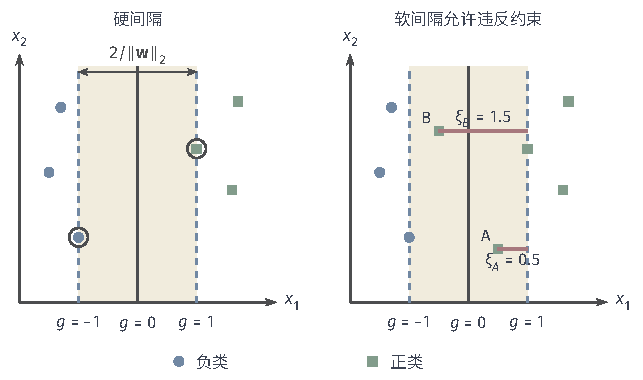
\includegraphics[width=108.850mm]{figures/04-classic-models/00-shared/tikz/classification-svm-margin/figure.pdf}
  \caption{硬间隔与软间隔的教学示意，坐标无量纲。蓝圆为负类，赭方为正类；两个面板都给定$\bm{w}=(1,0)^{\top}$、$b=-2$，黑色实线为决策边界$g=0$，蓝色虚线为间隔边界$g=\pm1$。单侧规范间隔为$1/\lVert\bm{w}\rVert_2=1$，两虚线总宽为$2/\lVert\bm{w}\rVert_2=2$；左图圈出间隔上的样本。右图红色线段直接标出松弛量：A位于$x_1=2.5$，正确分类但在间隔内，$\xi_A=0.5$；B位于$x_1=1.5$，已被错分，$\xi_B=1.5$。右图仅说明给定分界面下的最小松弛量，并非优化后的SVM最优解。}
  \label{fig:classification-svm-margin}
\end{figure}

消去$\bm{\xi}$，式\eqref{eq:classification-svm-soft-primal}等价于
\begin{equation}
  \min_{\bm{w},b}\quad
    \frac12\lVert\bm{w}\rVert_2^2
    +\lambda_{\mathrm{s}}\sum_{i=1}^n
       \max\{0,1-y_i g(\bm{x}_i)\}.
  \label{eq:classification-svm-hinge-objective}
\end{equation}
其中$\ell(z)=\max\{0,1-z\}$是\term{合页损失}（hinge loss）：达到目标间隔以后不再奖励更大的得分，间隔不足时线性增加惩罚。错误一侧的损失继续线性增加而不截断，保持了凸性。它把“最大间隔加违规代价”与“平方范数正则化加经验损失”联系起来。

惩罚参数的数值还依赖损失是求和还是取平均。将式\eqref{eq:classification-svm-hinge-objective}除以$n\lambda_{\mathrm{s}}$，等价目标是平均合页损失加$\lVert\bm{w}\rVert_2^2/(2n\lambda_{\mathrm{s}})$。所以在不同样本量或不同软件约定之间比较超参数时，应先统一归一化方式。较大的$\lambda_{\mathrm{s}}$允许模型付出更大范数来降低训练损失，较小的值更重视范数控制；范数和损失的这种取舍是否适合任务，需要结合数据、表示与验证结果判断。

软间隔的乘子上界来自松弛变量的最优性条件。分别为$1-\xi_i-y_i g(\bm{x}_i)\le0$与$-\xi_i\le0$引入$\alpha_i,\mu_i\ge0$，拉格朗日函数为
\[
  \begin{aligned}
    L={}&\frac12\lVert\bm{w}\rVert_2^2
       +\lambda_{\mathrm{s}}\sum_i\xi_i\\
      &+\sum_i\alpha_i
        \bigl[1-\xi_i-y_i(\bm{w}^{\top}\bm{x}_i+b)\bigr]
       -\sum_i\mu_i\xi_i.
  \end{aligned}
\]
关于$\bm{w},b$的驻点条件仍是式\eqref{eq:classification-svm-stationarity}，关于每个$\xi_i$则要求
\[
  \lambda_{\mathrm{s}}-\alpha_i-\mu_i=0.
\]
结合$\mu_i\ge0$，得到$0\le\alpha_i\le\lambda_{\mathrm{s}}$。取$\bm{w}=\bm{0}$、$b=0$和所有$\xi_i>1$可以严格满足两组不等式，因此不论数据是否可分，Slater条件都成立。消去原始变量后有
\begin{equation}
  \begin{aligned}
    \max_{\bm{\alpha}}\quad&
      \sum_{i=1}^n\alpha_i
       -\frac12\sum_{i,j=1}^n
         \alpha_i\alpha_j y_i y_j
         \bm{x}_i^{\top}\bm{x}_j\\
    \text{s.t.}\quad&
      \sum_{i=1}^n\alpha_i y_i=0,\\
    &0\le\alpha_i\le\lambda_{\mathrm{s}},
      \qquad i=1,\ldots,n.
  \end{aligned}
  \label{eq:classification-svm-soft-dual}
\end{equation}
对偶可行域非空且紧，目标连续，所以对偶最优值可以取得。原始形式同样有最优解；两类非空时，限制目标的水平集可控制$\bm{w}$与$\bm{\xi}$，再由两类约束控制$b$。

软间隔的互补松弛关系多了一组：
\begin{equation}
  \begin{aligned}
    &\alpha_i^{\ast}(m_i^{\ast}-1+\xi_i^{\ast})=0,\\
    &(\lambda_{\mathrm{s}}-\alpha_i^{\ast})\xi_i^{\ast}=0,\\
    &m_i^{\ast}\ge1-\xi_i^{\ast},\qquad \xi_i^{\ast}\ge0.
  \end{aligned}
  \label{eq:classification-svm-soft-kkt}
\end{equation}
联合原始与对偶可行性，可以逐项读出
\begin{equation}
  \begin{aligned}
    \alpha_i^{\ast}=0
      &\ \Longrightarrow\
        \xi_i^{\ast}=0,\quad m_i^{\ast}\ge1,\\
    0<\alpha_i^{\ast}<\lambda_{\mathrm{s}}
      &\ \Longrightarrow\
        \xi_i^{\ast}=0,\quad m_i^{\ast}=1,\\
    \alpha_i^{\ast}=\lambda_{\mathrm{s}}
      &\ \Longrightarrow\
        m_i^{\ast}=1-\xi_i^{\ast}\le1.
  \end{aligned}
  \label{eq:classification-svm-soft-cases}
\end{equation}
边界上的样本可以出现在三种乘子状态中：$\alpha_i^{\ast}=0$允许$m_i^{\ast}=1$，$\alpha_i^{\ast}=\lambda_{\mathrm{s}}$也允许$\xi_i^{\ast}=0$且$m_i^{\ast}=1$。反过来，$m_i^{\ast}>1$必有$\alpha_i^{\ast}=0$，$m_i^{\ast}<1$必有$\alpha_i^{\ast}=\lambda_{\mathrm{s}}$，而$m_i^{\ast}=1$时乘子可以是盒约束中的任意值，只要整体KKT系统成立。达到上界的乘子因此可能对应边界点、间隔内的正确样本或错分样本，需要结合$m_i^{\ast}$才能区分。

范数项依然只对$\bm{w}$严格凸，足以保证最优权重唯一，却不能保证偏置唯一。一个简单反例是两个输入都为零，标签分别为$+1$与$-1$。此时$\bm{w}^{\ast}=\bm{0}$，任意$b\in[-1,1]$都使总合页损失为$2$，因此都最优。该情形也说明，软间隔可能得到常值得分；只有$\bm{w}\ne\bm{0}$时，才可以继续用$1/\lVert\bm{w}\rVert_2$解释规范间隔的几何宽度。

若存在$0<\alpha_k^{\ast}<\lambda_{\mathrm{s}}$的\term{自由支持向量}（free support vector），它既参与决策又未碰到乘子上界，可用$m_k^{\ast}=1$恢复偏置。若没有这种样本，就应使用KKT给出的偏置区间。令$h_i=\sum_j\alpha_j^{\ast}y_j\bm{K}_{j,i}$，则$\alpha_i^{\ast}=0$要求$y_i(h_i+b)\ge1$，$\alpha_i^{\ast}=\lambda_{\mathrm{s}}$要求$y_i(h_i+b)\le1$。正标签的前一条件与负标签的后一条件给出下界，另两种组合给出上界；从两组界的交集中选择一个$b$，才是完整的恢复规则。该区间不一定收缩为单点。

SMO的一元目标与误差公式不变，但可行区间必须同时保证两个乘子都位于盒子内。令$s=y_i y_j$，新的$\alpha_j$区间为
\begin{equation}
  \begin{aligned}
    s=+1:\quad
    L&=\max\{0,\alpha_i^{(t)}+\alpha_j^{(t)}
                    -\lambda_{\mathrm{s}}\},\\
    H&=\min\{\lambda_{\mathrm{s}},
                    \alpha_i^{(t)}+\alpha_j^{(t)}\};\\
    s=-1:\quad
    L&=\max\{0,\alpha_j^{(t)}-\alpha_i^{(t)}\},\\
    H&=\min\{\lambda_{\mathrm{s}},
           \lambda_{\mathrm{s}}+\alpha_j^{(t)}-\alpha_i^{(t)}\}.
  \end{aligned}
  \label{eq:classification-svm-smo-soft-interval}
\end{equation}
这是由盒约束与等式约束共同截出的区间，通常小于$[0,\lambda_{\mathrm{s}}]$。使用式\eqref{eq:classification-svm-smo-update}剪裁并回代即可；当$\eta=0$时，这里的区间总是有限，可以直接比较端点目标。偏置仍按式\eqref{eq:classification-svm-smo-bias}计算，但优先使用更新后满足$0<\alpha_i<\lambda_{\mathrm{s}}$或$0<\alpha_j<\lambda_{\mathrm{s}}$的样本；二者都不自由时，可暂取两个候选偏置的平均，停止时再按全体KKT条件核验。

在可分数据上，足够大的有限惩罚就能使软间隔与硬间隔精确对应。取任意硬间隔最优乘子$\bm{\alpha}^{\mathrm{h}}$，若$\lambda_{\mathrm{s}}>\max_i\alpha_i^{\mathrm{h}}$，则硬间隔原始解连同$\bm{\xi}=\bm{0}$、$\bm{\alpha}^{\mathrm{h}}$和$\mu_i=\lambda_{\mathrm{s}}-\alpha_i^{\mathrm{h}}>0$满足软间隔KKT。由强对偶它也是软间隔最优解，而且正的$\mu_i$迫使所有最优松弛量为零。若数据不可分，则无论把惩罚增大到多少，都不能恢复一个本来就不存在的硬间隔可行解。

\paragraph{$\nu$-SVM：调节间隔与违反比例}
\label{sec:classification-svm-nu-extension}
软间隔惩罚系数衡量一单位间隔违反有多昂贵，却不能直接读成“允许多少训练样本违反间隔”。若希望调节参数与训练中的间隔错误比例、支持向量比例建立联系，可以考虑\term{$\nu$-SVM}（nu-support vector machine）。它把间隔阈值$\rho\geq0$也作为变量，在目标中用参数$\nu$奖励更大的阈值，同时惩罚平均松弛量：
\begin{equation}
  \begin{aligned}
    \min_{\bm{w},b,\rho,\bm{\xi}}\quad&
      \frac12\lVert\bm{w}\rVert_2^2-\nu\rho
      +\frac1n\sum_{i=1}^n\xi_i\\
    \text{满足}\quad&
      y_i(\bm{w}^{\top}\phi(\bm{x}_i)+b)\geq\rho-\xi_i,\\
    &\xi_i\geq0,\qquad \rho\geq0.
  \end{aligned}
  \label{eq:classification-nu-svm}
\end{equation}
消去原始变量后，可学习的仍是训练样本的非负系数，但对偶变为
\[
  \begin{aligned}
    \max_{\bm\alpha}\quad&-\frac12\sum_{i,j}\alpha_i\alpha_jy_iy_jK(\bm x_i,\bm x_j),\\
    \text{满足}\quad&0\leq\alpha_i\leq1/n,\quad
       \sum_i\alpha_i y_i=0,\quad\sum_i\alpha_i\geq\nu.
  \end{aligned}
\]
最后一个不等式来自原始问题中的$\rho\geq0$。固定核后可用凸二次规划求系数，再由原始约束和互补松弛恢复偏置及间隔阈值，预测仍对核展开得分取符号。这个目标与软间隔相似，却不是只把惩罚参数换一个名字。

使用时还需结合类别数量检查参数范围：两类训练样本数为$n_+$、$n_-$时，应限制$0<\nu\leq2\min(n_+,n_-)/n$。以下讨论达到精确最优、且最优间隔阈值$\rho^\ast>0$的非退化情形。记最优得分为$g^\ast$，满足$y_i g^\ast(\bm{x}_i)<\rho^\ast$的训练样本称为间隔违反样本；其中也包括已经分类正确、但尚未达到目标间隔的样本。此时，$\nu$是间隔违反样本比例的上界，也是非零对偶系数所对应支持向量比例的下界\scite{scholkopf2000nu}。

这两个方向可以从KKT条件读出。为间隔约束引入乘子$\alpha_i\geq0$。关于松弛变量的驻点条件给出$\alpha_i\leq1/n$；关于$\rho$的驻点条件与$\rho^\ast>0$的互补松弛关系给出
\[
  0\leq\alpha_i^\ast\leq\frac1n,
  \qquad \sum_{i=1}^{n}\alpha_i^\ast=\nu.
\]
这里仍有偏置的驻点条件$\sum_i\alpha_i^\ast y_i=0$，所以正、负两类的乘子总量相同，均为$\nu/2$。每项乘子至多为$1/n$，正类总量因而不超过$n_+/n$，负类总量不超过$n_-/n$。将这两项上界与$\nu/2$比较，就得到前面要求的$\nu\leq2\min(n_+,n_-)/n$；少数类的样本数量限制了两类能够共同承担的乘子总量。这也说明，上述类别数量条件与后面的比例解释都应结合当前模型及最优阈值条件检查。

令$E_\nu=\{i:y_i g^\ast(\bm{x}_i)<\rho^\ast\}$、$S_\nu=\{i:\alpha_i^\ast>0\}$。间隔违反样本的最优松弛量为正，因而乘子必须达到上界$1/n$；另一方面，要把每项至多$1/n$的非负乘子累加到$\nu$，至少需要$n\nu$个非零项。于是
\begin{equation}
  \frac{|E_\nu|}{n}\leq\nu\leq\frac{|S_\nu|}{n}.
  \label{eq:classification-nu-svm-proportions}
\end{equation}
例如，$n=100$、$\nu=0.2$且上述条件满足时，间隔违反样本至多有20个，支持向量至少有20个；这既不表示恰有20个错分样本，也不是对测试错误率的保证。若最优$\rho=0$，这里依据$\sum_i\alpha_i^\ast=\nu$得到的比例解释不能直接沿用。

固定核后，$\nu$-SVM与软间隔SVM使用同一得分族。它改变间隔的选取方式，不增加非线性特征，也仍需要检查核尺度、类别不平衡和独立验证误差。

\subsubsection{多分类：组合二分类器或联合学习}

\label{sec:classification-svm-multiclass}

二分类模型只需判断得分的正负；当候选类别超过两个时，还需要规定多个类别怎样竞争。一个直观的办法是把多分类问题拆成若干个“二选一”的小问题再把答案汇总；另一个办法是让所有类别在同一个优化目标里直接竞争。硬间隔、软间隔和核方法都能作为构件，但“拆成多个二分类器”与“直接优化多类间隔”会得到不同的训练目标。

现在将标签改为$y_i\in\{1,\ldots,C\}$，其中$C\ge3$，类别索引记为$c$。最直接的推广仍然保留二分类求解器，只改变训练任务的组织方式。\term{一对一}（one-vs-one，OvO）为每对类别$c<c'$训练一个分类器$h_{c,c'}$，仅使用标签为$c$或$c'$的样本，共有$C(C-1)/2$个模型。每个模型在这两个类别之间投一票，预测为
\[
  \hat y(\bm{x})
  =\argmax_{c\in\{1,\ldots,C\}}
     \sum_{c_1<c_2}\mathbb{1}\{h_{c_1,c_2}(\bm{x})=c\}.
\]
其中$c_1,c_2\in\{1,\ldots,C\}$，票数并列时采用预先约定的固定规则，例如选择较小类别编号。不同类别对可能作出不相容的局部判断，投票负责把这些判断汇总成一个输出，并不要求它们对应同一个全局概率模型。

\term{一对其余}（one-vs-rest，OvR）为每个类别$c$构造二分类标签：原标签为$c$时取$+1$，其余取$-1$。训练$C$个实值得分函数$g_c$后，使用
\[
  \hat y(\bm{x})=\argmax_{c\in\{1,\ldots,C\}}g_c(\bm{x}),
\]
并固定平局规则。即使所有得分都为负，或多个类别得分为正，这个最大值规则仍能给出类别。它比较的是独立模型的得分，得分尺度与训练中的类别不平衡可能影响比较，因此通常需要统一预处理、损失约定并评估各类别的错误，若要比较类别后验，还需建立并检验相应的概率映射。

图\ref{fig:classification-svm-multiclass}把四个类别展开成具体训练任务。沿着一列看，一对一中的每个类别只参与三个任务；一对其余中，每个样本都参与四个任务，但只有一个任务把它标为正类。沿着一行看，前者忽略不属于当前类别对的样本，后者把所有其他类别合并为负类。这种训练标签的差异，决定了两个组合器面对的子问题并不相同。

\begin{figure}[htbp]
  \centering
  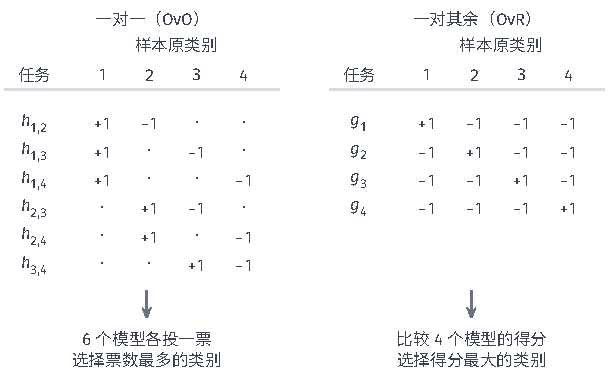
\includegraphics[width=104.027mm]{figures/04-classic-models/00-shared/tikz/classification-svm-multiclass/figure.pdf}
  \caption{四分类任务中的两种二分类组合方式。各行对应一个待训练模型，各列对应样本的原类别；$+1$和$-1$是为该任务重新编码的标签，点号表示该类样本不参与训练。一对一训练6个模型并汇总类别选票，一对其余训练4个模型并比较实值得分。图中给出训练与预测规则，不预设两种方法会产生相同的分类结果。}
  \label{fig:classification-svm-multiclass}
\end{figure}

OvO的模型多、单个训练子问题小，OvR的模型少、每个子问题使用全部样本；总成本因而取决于数据分布和求解器，不能只比较模型个数。

如果希望组合器能够容忍若干二分类判断错误，可以为每个类别安排一个彼此分离的编码。\term{纠错输出码}（error-correcting output codes，ECOC）将类别$c$表示成长度为$q$的码字$\bm{M}_{c,:}$，其中码本$\bm{M}\in\{-1,+1\}^{C\times q}$的各行互不相同，每列同时含两种符号。第$j$列定义一个二分类任务，样本$i$的训练标签为$\bm{M}_{y_i,j}$；训练后得到$q$个二分类器$h_j$。预测时形成输出码$\bm{h}(\bm{x})=(h_1(\bm{x}),\ldots,h_q(\bm{x}))$，再选择最近的类别码字：
\begin{equation}
  \begin{aligned}
    \hat y(\bm{x})
      &=\argmin_c d_{\mathrm{H}}
          \bigl(\bm{h}(\bm{x}),\bm{M}_{c,:}\bigr),\\
    d_{\mathrm{H}}(\bm{u},\bm{v})
      &=\sum_{j=1}^q\mathbb{1}\{u_j\ne v_j\}.
  \end{aligned}
  \label{eq:classification-svm-ecoc}
\end{equation}
这里的\term{汉明距离}（Hamming distance）就是两个码字不一致的位置数。要表示$C$个不同类别，至少需要$q\ge\lceil\log_2 C\rceil$；加入冗余位的目的，是增大不同类别之间的距离，而不只是增加分类器个数。Dietterich与Bakiri系统研究了这种将多分类转换为多个编码位学习问题的方法\scite{dietterich1995ecoc}。

纠错能力可以直接证明。记码本最小类间距离为$\Delta_{\min}$，若真实类别为$c$，输出码与$\bm{M}_{c,:}$相差$e$位，则对任意$c'\ne c$，三角不等式给出
\[
  d_{\mathrm{H}}(\bm{h},\bm{M}_{c',:})
  \ge d_{\mathrm{H}}(\bm{M}_{c,:},\bm{M}_{c',:})-e
  \ge\Delta_{\min}-e.
\]
只要$2e<\Delta_{\min}$，真实码字就比任何其他码字更近。因此至多$\lfloor(\Delta_{\min}-1)/2\rfloor$位错误可以被最近码字解码纠正。这个结论以实际错误位数为条件；若多个二分类器因为相同特征缺陷而同时犯错，冗余编码本身并不能保证错误位数足够小。

另一条路线不再训练彼此独立的二分类器，而是直接优化类别之间的竞争关系。\term{Crammer--Singer多类SVM}（Crammer--Singer multiclass SVM）要求真实类别得分至少比每个错误类别高一个单位间隔，从而在同一目标中学习所有类别权重。

令$\bm{W}=[\bm{w}_1,\ldots,\bm{w}_C]\in\mathbb{R}^{d\times C}$，使用带偏置的版本$g_c(\bm{x})=\bm{w}_c^{\top}\bm{x}+b_c$，相应优化问题为\scite{crammer2001multiclass}。
\begin{equation}
  \begin{aligned}
    \min_{\bm{W},\bm{b},\bm{\xi}}\quad&
      \frac12\sum_{c=1}^C\lVert\bm{w}_c\rVert_2^2
       +\lambda_{\mathrm{s}}\sum_{i=1}^n\xi_i\\
    \text{s.t.}\quad&
      g_{y_i}(\bm{x}_i)-g_c(\bm{x}_i)\ge1-\xi_i,
      \quad c\ne y_i,\\
    &\xi_i\ge0,\qquad i=1,\ldots,n.
  \end{aligned}
  \label{eq:classification-svm-crammer-singer}
\end{equation}
不使用偏置时固定$\bm{b}=\bm{0}$；使用偏置时，可加$\sum_c b_c=0$去掉共同平移的不识别性。消去松弛变量后，每个样本的损失为$\max\{0,\max_{c\ne y_i}[1+g_c(\bm{x}_i)-g_{y_i}(\bm{x}_i)]\}$，即惩罚最强错误竞争者超过允许差距的程度。预测仍取$\argmax_c g_c(\bm{x})$，并可将权重推广到核特征空间。这一凸目标可以用分解法求对偶，线性形式也可用次梯度训练：对每个样本先找得分最高的错误类别；若它违反单位间隔，损失对正确类权重贡献$-\lambda_{\mathrm s}\bm x_i$，对该竞争类贡献$+\lambda_{\mathrm s}\bm x_i$，其余类为零。累计全部样本的贡献，再加上范数项的梯度$\bm w_c$，沿负方向更新各类权重；偏置只累计损失项的相应标量贡献。最强竞争者并列时任选一个仍给出次梯度。这样，训练直接提高正确类相对于错误竞争者的得分，而不独立拟合每个“该类对其余类”的任务。

这一联合目标明确比较了类别之间的相对间隔，OvR则分别比较“该类”与“其余类”。二者的约束数、求解器和数据分解方式不同，训练成本与预测质量也要在相同数据和调参预算下评估。联合建模提供了不同的归纳偏好，并不构成相对于OvO或OvR的普遍性能排序。

这些多分类构造也改变了候选边界。线性OvR与联合多类SVM都按仿射得分的最大值判类，因此每类区域仍是半空间的交。OvO和ECOC先进行若干二分类再解码，各类区域可以由多个分区拼合。这种拼合能够表达单个半空间之外的区域，其能力由可用的二分类划分与解码方式共同决定。训练中的间隔保证若要用于整体分类，还需把错误的二分类比较与最终解码联系起来，不能直接取某个成员的风险作为组合器的风险。



\subsection{模型对比与总结}
\label{sec:classification-geometry-summary}

在同一组输入特征上的二分类问题中，LDA、感知机与线性SVM都用仿射得分形成半空间判断。只看边界的线性形状，无法知道权重来自哪里：LDA从类均值、共享协方差和先验形成得分；感知机在错分点出现时调整当前权重；SVM用范数与间隔损失比较候选边界。相同的得分形式因而不意味着相同的学习目标，也不意味着会从同一训练集选出相同边界。

若类条件高斯与共享协方差近似可信，LDA可以同时利用类内相关性并形成后验概率；样本不足以估计完整协方差时，需要收缩或更受限的协方差表示。感知机省去分布拟合，适合直接使用错误反馈作增量更新，但停止预算、访问顺序和历史参数的返回方式会影响结果。SVM在给定表示中显式权衡间隔与违反程度，代价是求解相应优化问题并选择惩罚强度。表\ref{tab:classification-linear-comparison}汇总这些选择条件。

\begin{table}[htbp]
  \centering
  \small
  \begin{tabularx}{\linewidth}{@{}>{\RaggedRight\arraybackslash}p{18mm}>{\RaggedRight\arraybackslash}X>{\RaggedRight\arraybackslash}X@{}}
    \toprule
    模型 & 边界由什么决定 & 主要条件与代价 \\
    \midrule
    LDA & 类均值、共享协方差与类先验 & 高斯假设支持概率解释；协方差估计需足够样本或正则化。 \\
    感知机 & 错分样本触发的权重更新 & 依赖访问顺序；不可分时需停止规则或变体。 \\
    线性 SVM & 范数与间隔损失的权衡 & 硬间隔要求可分；软间隔需选择惩罚强度。 \\
    核 SVM & 特征空间中的间隔 & 核定义相似性；训练与预测开销受样本数和支持向量数影响。 \\
    \bottomrule
  \end{tabularx}
  \caption{线性与核化分类器的比较。LDA 一行指共享协方差的高斯生成模型；Fisher 投影本身不要求高斯分布。比较时还需固定输入表示与评价口径。}
  \label{tab:classification-linear-comparison}
\end{table}

原坐标中的类别关系不能由仿射得分表达时，重复更新参数或调整惩罚都不能补上这种限制。核Fisher判别、核感知机与核SVM改用特征空间内积，分别保留类统计量比较、错分反馈与间隔选择这三种依据。核与输入尺度决定提供哪些关系，各自的学习目标再决定怎样使用这些关系。预测时是否需要保存全部训练样本、更新样本或支持向量，也随方法而异。

若还需要稀疏的概率核预测，相关向量机改用逐基函数的高斯先验与精度学习，其结构与训练见第\ref{sec:classification-rvm}节；它与SVM共享核展开形式，但不使用同一个间隔目标。

\section{基于邻域的分类}
\label{sec:classification-instances}

前面的线性分类器用一组全局权重决定边界。如果同一类别分布在几个相隔的区域，一条直线可能无法把它们同时与另一类分开。我们也可以暂不规定整条边界的形状，而在新输入附近寻找带标签的样本，用这些局部记录判断类别。这是$k$-NN分类的做法：保存训练实例，按距离找出邻居，再聚合标签。与回归中的响应平均相比，分类采用多数投票或局部类别比例。近邻表示和检索的基础见第\ref{sec:classic-overview-neighborhood}节，回归对应形式见第\ref{sec:regression-knn}节。

\subsection{$k$近邻分类（$k$-NN）}
\label{sec:classification-knn}

局部比较避开了预先选择全局边界，却留下一个问题：附近只取一个样本，还是让多个样本一起判断？最近的样本也可能带有噪声标签；增加邻居能平均这种波动，但范围过大又会把别处的类别混进来。近邻数因此决定了我们用多大范围的标签来描述当前输入。

Cover与Hart在1967年的论文中回顾了Fix与Hodges始于1951年报告的近邻判别研究：在所研究的条件下，让近邻数随样本量增长、同时让其占比趋于零，可以获得一致性。Cover与Hart则分析了始终只取一个最近邻时，极限错误率与贝叶斯风险之间的界。前者研究增长近邻数怎样平均标签噪声，后者刻画单个邻居仍保留多少判别信息\scite{coverhart1967}。

\subsubsection{模型结构}
\label{sec:classification-knn-structure}

给定训练集$D_n=\{(\bm{x}_i,y_i)\}_{i=1}^n$、距离$\rho$以及$1\leq k\leq n$，用$N_k(\bm{x})\subseteq\{1,\ldots,n\}$表示查询$\bm{x}$的$k$个最近邻索引。预测规则为
\begin{equation}
  \hat h_{n,k}(\bm{x})
  =\argmax_{c\in\{1,\ldots,C\}}
  \sum_{i\in N_k(\bm{x})}\mathbb{1}\{y_i=c\}.
  \label{eq:classification-knn-vote}
\end{equation}
距离相同时，按预先约定、独立于标签的顺序选取邻居；类别票数并列时也使用固定规则。多分类在奇数$k$时也可能出现票数并列，因此两种平局都需要明确规则。

式\eqref{eq:classification-knn-vote}也可以理解为估计查询附近的类别比例：
\begin{equation}
  \hat\eta_{n,c}(\bm{x})
  =\frac{1}{k}\sum_{i\in N_k(\bm{x})}\mathbb{1}\{y_i=c\},
  \qquad
  \hat h_{n,k}(\bm{x})=\argmax_c\hat\eta_{n,c}(\bm{x}).
  \label{eq:classification-knn-posterior}
\end{equation}
比例估计解释了投票为什么可能有效：若邻域内的条件类别分布变化不大，邻居标签就能提供关于当前输入的统计证据。局部比例的误差取决于邻域大小与标签噪声，概率质量需通过样本外数据检验。

图~\ref{fig:classification-knn-neighborhood}固定训练点和查询，只改变参与投票的近邻数。取查询$\bm{x}=(0,0)$，样本1、3、4、6属于类1，其余样本属于类2。按欧氏距离计算，七个样本到查询的平方距离依编号为$1,2,2.5,4.25,5,9,10.25$，因此编号也表示由近到远的次序。

$k=1$时只有样本1投票，查询被判为类1；$k=5$时样本1至5投票，其中类1有三票、类2有两票，预测仍为类1。两幅图中的圆分别经过第1和第5个邻居，半径为$1$和$\sqrt5$。圆表示当前查询的证据范围，整个平面上的分类边界则由各查询的投票共同决定。比较两个$k$的准确性还需要查询的真实标签。

\begin{figure}[htbp]
  \centering
  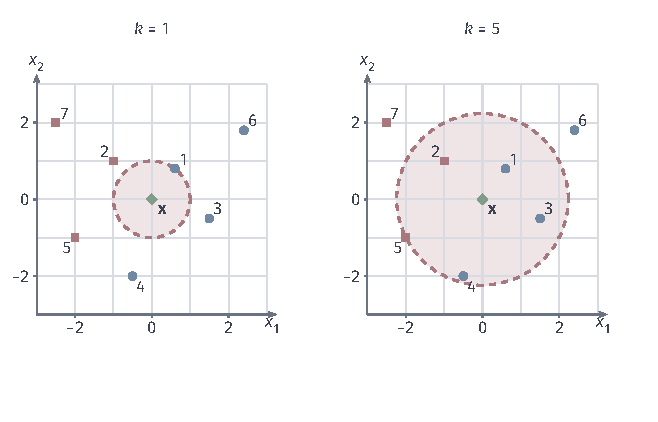
\includegraphics[width=111.404mm]{figures/04-classic-models/00-shared/tikz/classification-knn-neighborhood/figure.pdf}
  \caption{同一查询下的近邻范围与投票变化。教学构造取$n=7$、$d=2$、无量纲坐标和欧氏距离，查询为$\bm{x}=(0,0)$；两图的样本、编号及坐标尺度完全相同。蓝色圆点表示类1，红色方点表示类2，绿色菱形表示查询，红色虚线圆表示包含边界的近邻范围。左图$k=1$、半径$1$，蓝、红票数为$1:0$；右图$k=5$、半径$\sqrt5$，票数为$3:2$，因此判为蓝色类。各邻居等权投票，距离和票数均无并列；点的位置、标签与参数均为人为设定，不代表真实数据实验。}
  \label{fig:classification-knn-neighborhood}
\end{figure}

\subsubsection{参数学习}
\label{sec:classification-knn-learning}

基本$k$-NN分类没有固定维数参数的优化过程，但需要确定输入表示、距离、近邻数及检索方式。“非参数化”是指预测关系不局限于一个固定有限维参数族；它仍有超参数，预处理和模型选择也属于学习。

距离决定哪些样本会参与投票。对数值特征，欧氏距离$\rho(\bm{x},\bm{z})=\lVert\bm{x}-\bm{z}\rVert_2$容易计算，却会放大数值范围较大的坐标。收入和年龄共同作为特征时，直接使用原始单位会让收入差异主导距离。标准化、按业务意义设定尺度或学习特征权重都可改变这一点；不同特征的重要性可通过任务知识或训练数据确定。标准化参数只能从训练集估计，交叉验证时应在各训练折内重新拟合，避免验证信息提前进入距离。

类别型特征可采用\term{汉明距离}（Hamming distance），按不同取值的坐标数比较，而不能把任意类别编码的数字差当成有意义的远近。文本的TF--IDF等稀疏向量常比较余弦相似度，强调方向而非长度；$1$减余弦相似度一般不满足三角不等式，不能直接套用所有度量空间结论。对非零向量作单位长度归一化后，按余弦相似度排序与按欧氏距离排序等价，此时可用欧氏空间中的解释。

若特征之间相关，可以考虑\term{马氏距离}（Mahalanobis distance），用协方差调整方向上的尺度：
\begin{equation}
  \rho_{\mathrm{M}}(\bm{x},\bm{z})^2
  =(\bm{x}-\bm{z})^\top
   \bm{\Sigma}^{-1}(\bm{x}-\bm{z}),
  \label{eq:classification-mahalanobis}
\end{equation}
其中$\bm{\Sigma}\in\mathbb{R}^{d\times d}$须正定。样本不足时协方差估计可能奇异，需要正则化；整体协方差也不一定符合分类所需的相似性。

近邻数$k$控制局部平均的范围。$k=1$时，一个错误标签就会影响邻近查询；增加邻居可平均这类波动，也会混入更远区域并削弱局部细节。因此$k$的选择需要结合类别比例、局部密度与距离表示，在训练集内部验证。$k\approx\sqrt n$可以作为搜索起点，最终选择依据相同评价条件下的误差。

检索代价需要区分距离计算与邻居选择。对一个$d$维稠密查询，朴素扫描$n$个训练样本计算距离需$O(nd)$；若再把所有距离排序，总代价为$O(nd+n\log n)$。采用线性选择算法得到最小的$k$项，再作投票，可达$O(nd+n+k)$；使用大小为$k$的堆则需$O(nd+n\log(k+1)+k)$。因此，通常所说的$O(nd)$朴素预测复杂度隐含了无需完整排序的选择方法。训练集的存储为$O(nd)$，批量计算、硬件、精度要求和延迟预算共同决定这种实现的可用规模。

KD树或球树（ball tree）等精确索引通过空间划分排除不可能更近的样本。低维且分布有利时，它们可以减少访问量；最坏情形仍会检查大部分样本。索引保留原预测规则，选择时比较建索引成本、内存和实际查询时间，维数的影响需结合数据分布测量。

对高维大规模数据，还可以用\term{近似最近邻检索}（approximate nearest-neighbor search）交换少量检索误差与计算收益。局部敏感哈希（locality-sensitive hashing, LSH）让相近向量较可能进入同一哈希桶；分层可导航小世界图（hierarchical navigable small world, HNSW）沿多层邻接图逐步寻找候选；倒排文件与乘积量化（inverted file with product quantization, IVF--PQ）先缩小候选分区，再用压缩编码近似距离。这些方法的搜索预算和压缩程度会改变邻居集合，需同时检查邻居召回率与最终分类误差。以下理论以精确检索为前提，不直接覆盖任意近似索引。

\subsubsection{理论分析}
\label{sec:classification-knn-theory}

\paragraph{表达能力}
固定$n$、$k$及欧氏距离后，一个候选规则由$n$个锚点的位置与类别共同规定：查询时取最近的$k$个锚点，再按既定平局规则比较票数。考察所有可能的锚点位置与类别，才能说明这一规则族能够表达哪些目标。每个候选都是分段常值函数；邻居集合只在锚点的等距平面处改变，同一邻居集合给出相同票数。

锚点可以让一个类别占据几个分离的区域。例如，$k=1$时将四个锚点放在前面的异或输入$(\pm1,\pm1)$上，并赋予相应类别，坐标轴便把平面划成四个最近锚点区域；四个开象限的类别可全部吻合异或目标。更一般地，若各目标类别对应的输入集合都紧致，不同类别集合之间的距离至少为$\Delta>0$，可在每类选取有限个锚点，使该类每个输入到同类锚点的距离小于$\Delta/2$。当$n$足以容纳这一覆盖时，异类锚点至少相距$\Delta$，这组1-NN候选便能精确表示整个目标支持上的类别。

有限锚点仍限制了边界形状。在平面上按单位圆的内外区分类别时，有限条等距直线不能拼成整条圆周，任一有限锚点候选都无法处处吻合这个目标。若输入表示又把不同目标类别映到同一点，所有基于该表示的候选都会对它们给出相同判断。

票数比例还有独立于分区形状的限制。固定$k$时，每类比例只能取$0,1/k,\ldots,1$，不能精确表示任意后验概率。例如两类、$k=3$且真实正类后验恒为$3/10$时，任一候选在每个输入处的概率差都至少为$1/30$。增加锚点数可以提供更多空间分区，却不改变这一固定的概率刻度。

\paragraph{收敛性}
标准$k$-NN保存训练实例，给定距离和邻居数后没有参数优化过程，也就没有迭代找到最优参数的保证或速率。精确检索与投票能直接执行已定义的预测规则；朴素稠密实现为每个查询计算$n$个距离，约需$O(nd)$运算，再选择近邻。近似检索降低计算成本时，漏检或错检造成的误差必须另行评价。

\paragraph{泛化性}
位置接近仍可能伴随标签差异。两个相同输入在类别重叠或标签噪声下，也可独立产生不同标签。因此先规定训练集、查询与标签的随机性，再将邻居位置的极限联系到条件类别分布和分类风险。

设训练样本与测试点$(\bm{X},Y)$独立同分布于$\mathbb{R}^d\times\{1,\ldots,C\}$，$P_X$为输入边缘分布，$C\geq2$。令
\begin{equation}
  \eta_c(\bm{x})=\mathbb{P}(Y=c\mid\bm{X}=\bm{x}),
  \qquad
  r^\ast(\bm{x})=1-\max_c\eta_c(\bm{x}).
  \label{eq:classification-local-bayes-risk}
\end{equation}
沿用\term{贝叶斯风险}（Bayes risk）记号$R^\ast=\mathbb{E}_{\bm{X}}r^\ast(\bm{X})$。为区分近邻规则在一份训练集上的风险和它对训练抽样的平均表现，分别记为
\begin{align}
  L_{n,k}(D_n)
  &=\mathbb{P}\{\hat h_{n,k}(\bm{X})\neq Y\mid D_n\},
  \label{eq:classification-knn-conditional-risk}\\
  R_{n,k}&=\mathbb{E}_{D_n}L_{n,k}(D_n).
  \label{eq:classification-knn-expected-risk}
\end{align}
若打破距离并列采用独立随机化，以上期望同时包含该随机化。下面的Cover--Hart界针对$R_{n,1}$的极限，不是任意有限$n$的风险上界，也不是每份训练集条件风险的逐一保证。

先看局部比例的估计偏差。给定邻居输入后，等权票数比例的条件期望为$k^{-1}\sum_{r=1}^k\eta_c(\bm x_{(r)})$。若存在常数$L_\eta\geq0$，使$|\eta_c(\bm x)-\eta_c(\bm z)|\leq L_\eta\|\bm x-\bm z\|_2$，并记最远邻居距离为$r_k(\bm x)$，则
\[
  \left|\frac1k\sum_{r=1}^k\eta_c(\bm x_{(r)})
                 -\eta_c(\bm x)\right|
       \leq L_\eta r_k(\bm x).
\]
这一式子只控制条件均值的偏差，标签抽样还会使实际票数波动；下面的风险结论需要把两者一起处理。

先说明足以支撑极限计算的一组分布条件。使用固定的欧氏距离，精确寻找最近邻，邻居选择不依赖标签；对$P_X$几乎处处的非原子点$\bm{x}$，各$\eta_c$在该点相对于$P_X$的支撑集连续。所谓原子点是$P_X(\{\bm{x}\})>0$的点，它不需要这里的连续性要求。该条件不要求输入分布有密度，更不要求每个欧氏空间位置都有正密度，但它也不只是“条件概率存在”。

\begin{lemma}[最近邻风险的极限]
  \label{lem:classification-nearest-neighbor-limit}
  在上述抽样、检索与连续性条件下，最近邻位置几乎必然趋于查询位置，并且
  \begin{equation}
    R_{1,\infty}:=\lim_{n\to\infty}R_{n,1}
    =\mathbb{E}_{\bm{X}}\left[
      1-\sum_{c=1}^{C}\eta_c(\bm{X})^2
    \right].
    \label{eq:classification-nearest-neighbor-limit}
  \end{equation}
\end{lemma}

\begin{proof}
  将训练集看作同一无穷独立样本序列的前$n$项。固定支撑集中的查询$\bm{x}$，用$I_n$表示最近邻索引，用$B(\bm{x},\varepsilon)$表示半径$\varepsilon>0$的开球。支撑集的定义保证该球有正概率，因此
  \[
    \mathbb{P}\{\|\bm{X}_{I_n}-\bm{x}\|_2\geq\varepsilon\}
    =\bigl[1-P_X(B(\bm{x},\varepsilon))\bigr]^n
    \longrightarrow0.
  \]
  最近邻距离随$n$不增，对$\varepsilon=1,1/2,1/3,\ldots$分别取极限，即得$\bm{X}_{I_n}\to\bm{x}$几乎必然成立。欧氏空间具有可数拓扑基，不在支撑集中的点可被可数个零概率开集覆盖，故支撑集本身具有$P_X$概率1。若$\bm{x}$为原子点，训练序列几乎必然在有限步后出现$\bm{x}$，此后最近邻距离一直为零。

  对非原子点，由连续性得到$\eta_c(\bm{X}_{I_n})\to\eta_c(\bm{x})$；对原子点，这个等式最终直接成立。最近邻索引只依赖输入及与标签独立的平局约定。给定查询和所有训练输入后，测试标签与选中的训练标签独立，选中标签属于$c$的概率为$\eta_c(\bm{X}_{I_n})$。故对训练集平均的条件错误率为
  \[
    r_n(\bm{x})
    =1-\sum_{c=1}^{C}\eta_c(\bm{x})
       \mathbb{E}\bigl[\eta_c(\bm{X}_{I_n})\bigr],
  \]
  这里的期望针对固定查询时的训练输入及邻居选择随机性。由于后验概率有界，可用支配收敛定理得到
  \[
    r_n(\bm{x})\longrightarrow
    r_\infty(\bm{x})
    :=1-\sum_{c=1}^{C}\eta_c(\bm{x})^2.
  \]
  再利用$0\leq r_n(\bm{x})\leq1$，对$\bm{x}$积分并交换极限与期望，就得到式\eqref{eq:classification-nearest-neighbor-limit}。
\end{proof}

极限中的平方项来自两次独立的类别抽取，而不是说最近邻标签本身几乎必然收敛。位置接近保证的是选中标签的条件分布接近查询的条件分布，单次标签抽样的波动仍然存在。

要平均掉这部分噪声，需要让参与投票的邻居数增加；要避免把远处结构混入，又需要邻居只占全部训练样本的越来越小一部分。令$k=k_n$满足$k_n\to\infty$且$k_n/n\to0$。Stone的非参数一致性结果在固定有限维欧氏空间中建立了近邻条件概率估计的积分收敛，也就是对训练集与查询取平均后，估计的绝对误差趋于零；这为后面的风险分析提供了依据\scite{stone1977consistent}。

对精确欧氏近邻，距离并列时可按与数据独立的随机排列选取，类别票数并列时按固定类别顺序决定。对每个$c$，这样的近邻估计满足
\begin{equation}
  \mathbb{E}_{D_n,\bm{X}}
  \bigl|\hat\eta_{n,c}(\bm{X})-\eta_c(\bm{X})\bigr|
  \longrightarrow0.
  \label{eq:classification-knn-posterior-consistency}
\end{equation}
这一结论对$\mathbb{R}^d$上任意固定联合分布成立，不需要前面为简化Cover--Hart证明而采用的逐点连续性条件。其一般证明使用欧氏空间的覆盖性质，不能只用一句普通大数定律代替，因为邻居样本是根据查询和输入位置选择出来的。

在前述连续性条件下，可以直接看出式\eqref{eq:classification-knn-posterior-consistency}的两个来源。给定训练输入，记
\[
  \bar\eta_{n,c}(\bm{x})
  =\frac{1}{k_n}\sum_{i\in N_{k_n}(\bm{x})}\eta_c(\bm{X}_i).
\]
邻居标签在给定输入后独立，所以
\[
  \mathbb{E}\!\left[
    |\hat\eta_{n,c}(\bm{x})-\bar\eta_{n,c}(\bm{x})|
    \,\middle|\,\bm{X}_1,\ldots,\bm{X}_n
  \right]\leq\frac{1}{2\sqrt{k_n}}.
\]
上界来自Bernoulli变量的方差不超过$1/4$及Cauchy--Schwarz不等式。它控制标签抽样波动。对任意有正概率的查询邻域，落入其中的样本比例几乎必然趋向该邻域的概率；由于$k_n/n\to0$，最终会有至少$k_n$个训练样本落入其中。因此，第$k_n$个邻居的距离趋于零。后验连续时，$\bar\eta_{n,c}(\bm{x})-\eta_c(\bm{x})$趋于零；在原子点，最终选中的$k_n$个输入都可等于该点。结合有界性与支配收敛，就得到这组较强正则性条件下的积分收敛。Stone的结论把同一估计分析扩展到了不连续后验。

已有的极限计算还需要与最优分类错误比较，才能说明近邻规则的预测保证。固定$k=1$时，Cover--Hart定理比较引理~\ref{lem:classification-nearest-neighbor-limit}中的极限局部错误与最优局部错误；让$k_n$增长时，则可用式\eqref{eq:classification-knn-posterior-consistency}控制相对于贝叶斯决策多出的错误。这两种风险保证都对训练集和独立测试点取平均。

\begin{theorem}[1-NN在二分类条件下的渐近期望风险界]
  \label{thm:classification-cover-hart-binary}
  在引理~\ref{lem:classification-nearest-neighbor-limit}的条件下，若$C=2$，则
  \begin{equation}
    R^\ast\leq R_{1,\infty}
    \leq2R^\ast(1-R^\ast)\leq2R^\ast.
    \label{eq:classification-cover-hart-binary}
  \end{equation}
\end{theorem}

\begin{proof}
  固定$\bm{x}$，记$p=\eta_1(\bm{x})$，则$\eta_2(\bm{x})=1-p$，$r^\ast(\bm{x})=\min(p,1-p)$。引理给出
  \begin{align*}
    r_\infty(\bm{x})
    &=1-p^2-(1-p)^2\\
    &=2p(1-p)\\
    &=2r^\ast(\bm{x})\bigl[1-r^\ast(\bm{x})\bigr].
  \end{align*}
  由于$0\leq r^\ast(\bm{x})\leq1/2$，有$2(1-r^\ast(\bm{x}))\geq1$，所以$r_\infty(\bm{x})\geq r^\ast(\bm{x})$。对输入取期望得到下界。对于上界，
  \begin{align*}
    R_{1,\infty}
    &=2R^\ast-2\mathbb{E}_{\bm{X}}[r^\ast(\bm{X})^2]\\
    &\leq2R^\ast-2(R^\ast)^2\\
    &=2R^\ast(1-R^\ast).
  \end{align*}
  不等式利用$\mathbb{E}[Z^2]\geq(\mathbb{E}Z)^2$，也就是对凹函数$2z(1-z)$使用Jensen不等式。再用$1-R^\ast\leq1$得到两倍上界。
\end{proof}

多分类时，不能沿用二类的精确表达式$2p(1-p)$，因为非最大类别的概率还可以在多个类别之间分配。需要控制的是：固定最大后验概率以后，其余类别的概率平方和最小能是多少。

\begin{theorem}[1-NN在多分类条件下的渐近期望风险界]
  \label{thm:classification-cover-hart-multiclass}
  在引理~\ref{lem:classification-nearest-neighbor-limit}的条件下，对任意有限$C\geq2$，
  \begin{equation}
    R^\ast\leq R_{1,\infty}
    \leq R^\ast\left(2-\frac{C}{C-1}R^\ast\right)
    \leq2R^\ast.
    \label{eq:classification-cover-hart-multiclass}
  \end{equation}
\end{theorem}

\begin{proof}
  固定$\bm{x}$并简记$r=r^\ast(\bm{x})$。取$c^\ast$使$\eta_{c^\ast}(\bm{x})=1-r$，其余$C-1$类的概率之和为$r$。由Cauchy--Schwarz不等式，
  \[
    r^2
    =\left(\sum_{c\neq c^\ast}\eta_c(\bm{x})\right)^2
    \leq(C-1)\sum_{c\neq c^\ast}\eta_c(\bm{x})^2.
  \]
  因而
  \begin{align*}
    \sum_{c=1}^{C}\eta_c(\bm{x})^2
    &\geq(1-r)^2+\frac{r^2}{C-1},\\
    r_\infty(\bm{x})
    &\leq1-(1-r)^2-\frac{r^2}{C-1}\\
    &=2r-\frac{C}{C-1}r^2.
  \end{align*}
  这一步的等号在其余类别的概率都等于$r/(C-1)$时成立。记$g_C(r)=2r-Cr^2/(C-1)$，它在$0\leq r\leq1-1/C$上为凹函数。对输入取期望并用Jensen不等式，
  \[
    R_{1,\infty}
    \leq\mathbb{E}_{\bm{X}}g_C(r^\ast(\bm{X}))
    \leq g_C(R^\ast).
  \]
  去掉非负的二次项得到$R_{1,\infty}\leq2R^\ast$。另一方面，$\eta_c(\bm{x})\leq1-r$，故
  \[
    \sum_{c=1}^{C}\eta_c(\bm{x})^2
    \leq(1-r)\sum_{c=1}^{C}\eta_c(\bm{x})=1-r.
  \]
  于是$r_\infty(\bm{x})\geq r$，积分后得到$R_{1,\infty}\geq R^\ast$。
\end{proof}

这两个界不要求某个参数化类别分布，却仍依赖已列出的抽样和分布正则性条件。若$R^\ast=0$，界给出1-NN的期望风险趋于零；若后验概率在所有位置都为$(0.8,0.2)$，则$R^\ast=0.2$而$R_{1,\infty}=0.32$。后一个教学计算表明，单个近邻即使位于查询附近，也仍带有一次标签抽样的噪声，因此1-NN一般不能使期望风险趋于贝叶斯风险。

上面的后验估计结果能够推出近邻分类器的\term{贝叶斯一致性}（Bayes consistency）。下面把由局部票数到新样本风险的最后一步写出，并保留有限样本中局部估计偏差与标签波动的影响。
\begin{theorem}[$k$-NN分类在后验光滑条件下的期望风险界]
  \label{thm:classification-knn-risk}
  设$d,C$固定，训练样本独立同分布于$\mathbb R^d\times\{1,\ldots,C\}$，测试点独立来自同一分布。使用精确欧氏近邻，距离平局按与数据独立的随机排列处理，类别票数平局按固定次序处理。对预定的$1\leq k\leq n$，令
  \[
    B_{n,k}=\sum_{c=1}^C\mathbb E_{D_n,\bm X}
       \left|\frac1k\sum_{i\in N_k(\bm X)}
          \eta_c(\bm X_i)-\eta_c(\bm X)\right|.
  \]
  返回多数投票分类器$\hat h_{n,k}$后，有
  \[
    0\leq R_{n,k}-R^\ast
      \leq2\sum_{c=1}^C\mathbb E_{D_n,\bm X}
          |\hat\eta_{n,c}(\bm X)-\eta_c(\bm X)|
      \leq2B_{n,k}+\frac C{\sqrt k}.
  \]
  若$k=k_n\to\infty$且$k_n/n\to0$，则$R_{n,k_n}\to R^\ast$。
\end{theorem}
\begin{proof}
对固定查询和训练集，令$c^\ast$为真实后验最大的类别，$\hat c=\hat h_{n,k}(\bm{x})$。由于$\hat\eta_{n,\hat c}\geq\hat\eta_{n,c^\ast}$，
\begin{align*}
  \eta_{c^\ast}(\bm{x})-\eta_{\hat c}(\bm{x})
  &\leq|\eta_{c^\ast}(\bm{x})-\hat\eta_{n,c^\ast}(\bm{x})|\\
  &\quad+|\hat\eta_{n,\hat c}(\bm{x})-\eta_{\hat c}(\bm{x})|\\
  &\leq2\sum_{c=1}^{C}
    |\hat\eta_{n,c}(\bm{x})-\eta_c(\bm{x})|.
\end{align*}
左侧就是相对于贝叶斯决策多出的条件错误率。对训练集与测试输入取期望，得到定理的第一个上界。给定所有输入后，选中的$k$个标签相互独立；每类票数比例的条件方差至多为$1/(4k)$。因此它与邻域内真实后验平均值的期望绝对偏差至多为$1/(2\sqrt k)$。用三角不等式把这一波动与$B_{n,k}$中的局部偏差相加，再对类别求和，就得到第二个上界。最后使用式\eqref{eq:classification-knn-posterior-consistency}和类别数有限，得到
\begin{equation}
  R_{n,k_n}\longrightarrow R^\ast,
  \qquad k_n\to\infty,\quad k_n/n\to0.
  \label{eq:classification-knn-bayes-consistency}
\end{equation}
\end{proof}

有限样本界中的$B_{n,k}$衡量邻域内的后验平均值与查询处后验的差别；$C/\sqrt k$来自标签抽样波动。增加$k$能减小后者，却可能扩大邻域、增大前者，所以只增加票数并不足够。极限结论对训练集和查询平均；由$L_{n,k_n}(D_n)-R^\ast\geq0$，还可推出条件风险依概率趋于$R^\ast$。几乎必然收敛、逐点标签稳定等更强结论需要另外的条件与论证；后验平局时，不同标签本就可能具有相同的最小风险。

\subsubsection{优化泛化能力}

\paragraph{优化邻居的距离表示}
马氏距离可以校正输入的整体尺度和相关性，但按全体样本的协方差构造时，并未区分哪些近邻应当同类、哪些应当异类。\term{度量学习}（metric learning）把已知标签纳入距离选择。Weinberger与Saul研究的\term{大间隔最近邻}（large margin nearest neighbor, LMNN）先指定同类目标邻居，再学习线性变换：让目标邻居接近，同时用间隔约束排开可能干扰局部判断的异类样本\scite{weinberger2009}。

Goldberger等研究的\term{近邻成分分析}（neighbourhood components analysis, NCA）则对邻居选择作概率化处理，通过提高留一预测中选到同类样本的概率学习线性变换\scite{goldberger2004nca}。LMNN围绕预定目标邻居组织距离和间隔，NCA围绕概率化的邻居选择组织预测目标；两者都可以改变坐标间的组合及邻居顺序，训练准则却不同。额外拟合也带来训练成本与过拟合风险，学得的度量需要与$k$一起在未参与拟合的数据上评价，以检验监督变换是否保留了新样本的类别关系。

\paragraph{优化邻居的投票权重}
等权投票把选中的邻居一视同仁，却没有使用它们距离查询的差别。例如，在一个教学构造中，三个邻居的距离依次为$0.1$、$0.9$、$1$，最近者属于类1，另外两者属于类2。等权投票选择类2；如果我们认为近处标签更能反映查询的类别，就可以让远处两票的影响小一些。\term{加权$k$近邻}（weighted $k$-nearest neighbors）据此让不同邻居贡献不同票数：
\begin{equation}
  \hat h(\bm{x})=\argmax_c
  \sum_{i\in N_k(\bm{x})}
  w_i(\bm{x})\mathbb{1}\{y_i=c\},
  \qquad w_i(\bm{x})\geq0.
  \label{eq:classification-weighted-knn}
\end{equation}
至少需要一个权重为正。Dudani在1976年研究了按邻居距离范围作线性缩放的加权方案，使最近邻具有最大权重、较远邻居的权重逐渐减小\scite{dudani1976weighted}。

具体地，把邻居按距离排序为$\delta_1\leq\cdots\leq\delta_k$，第$r$个邻居的权重取
\begin{equation}
  w_r=
  \begin{cases}
    \dfrac{\delta_k-\delta_r}{\delta_k-\delta_1},
      & \delta_k>\delta_1,\\[4pt]
    1, & \delta_k=\delta_1.
  \end{cases}
  \label{eq:classification-dudani-weights}
\end{equation}
前面的三个邻居按式\eqref{eq:classification-dudani-weights}得到权重$1$、$1/9$、$0$，查询便改判为类1。这说明距离加权怎样改变局部证据，并不说明新判断一定正确：最近的标签也可能有误。

另一类常用选择是逆距离权重或高斯形权重$\exp(-\delta_r^2/(2h^2))$，其中$h>0$控制衰减尺度。逆距离形式遇到零距离必须处理，例如只在零距离样本中投票，避免除零。距离加权可能减少远邻干扰，也可能放大近处噪声。加权后的硬类别输出仍在最大票数类别变化时跳变，其对$k$的敏感程度需要另行评价。权重长期集中在少数记录上时，一个错误标签就可能主导判断；用标签学习距离或权重时，也需要在未参与拟合的数据上检查这种选择。

\subsubsection{小结}
\label{sec:classification-knn-summary}

$k$-NN保留训练实例，用查询附近的标签判断类别。表示与距离先决定哪些记录算邻居，近邻数再决定证据范围；局部类别变化明显时，过大的邻域会混入其他区域，标签噪声较多时，单个邻居又可能主导判断。

等权投票之外，距离加权让较近记录贡献更多票数，监督度量则利用标签调整邻居的位置关系。前者可能放大近处的错误标签，后者增加训练和验证成本；两种改动都需要与近邻数一起选择。检索索引减少访问量，近似检索还可能改变返回的邻居，应同时检查查询成本与分类质量。

高维或无关坐标可能使所用距离缺少类别信息。应先检查特征表示和样本覆盖，再决定是否增加邻域、学习距离或改用其他表示，不能只靠增加票数补偿缺失的信息。

\subsection{模型对比与总结}
\label{sec:classification-instances-comparison}

近邻方法的几个选择分别处理不同问题：距离加权调节已经选中记录的影响，监督度量改变哪些记录能够入选，检索方法控制访问这些记录的成本。需要保留细小或分散的类别区域时，实例库提供了局部依据；存储与查询负担随样本增加时，则要判断能否用更少的代表点概括这些区域。

\term{学习向量量化}（learning vector quantization, LVQ）采用带类别的\term{原型向量}（prototype vector）代替全部实例：原型是可移动的代表点，不必对应某条观测；基本更新把最近的同类原型拉向样本，把异类原型推远。Kohonen发展的这一方法把模型规模交给原型数控制，但每类需要多少代表点，仍取决于类内区域是否分散，训练也受初始化和访问顺序影响\scite{kohonen2001som}。

若每类确实围绕单个中心分布，\term{最近质心分类器}（nearest centroid classifier）还可以直接用类内均值作为代表，预测时比较到这些中心的距离。它省去移动原型的训练，却只能保留一个中心；一个类别包含几处分离区域时，均值可能落在另一类附近。多原型与单质心因此是在存储、查询成本和类别几何之间作不同取舍，应在相同验证数据上比较。

\section{基于树与规则的分类}
\label{sec:classification-trees}

有些类别关系由局部条件决定：先检查一个特征，只有条件不满足时才需要查看另一个特征。例如图\ref{fig:classification-tree-partition}中的教学分类规则，在左半区域一律输出类1，在右半区域才由第二个坐标决定类别。一个全局线性得分不能精确表达整片区域中的这两段分界。分类树沿用第\ref{sec:classic-overview-tree-rules}节的条件分支，把输入逐步送入不同区域，再在叶节点输出类别或类别比例；路径中的先后测试使后续条件只在相应区域生效。

沿用训练集$D_n=\{(\bm{x}_i,y_i)\}_{i=1}^n$，其中输入有$d$个特征，$y_i\in\{1,\ldots,C\}$。本节允许特征是数值型或类别型，用$D\subseteq D_n$表示到达某个节点的训练样本。建树需要同时确定测试特征、阈值或取值分组，以及叶节点的输出，并非只估计一组预先固定的数值参数。常见做法是在当前节点选择一个能改善类别划分的测试，再递归处理各个子集；为避免把偶然差异也变成分支，还要限制生长或在生长后\term{剪枝}（pruning），即删除缺少预测收益的子树。

图~\ref{fig:classification-tree-partition}把同一个分类器分别画成区域和条件树。在$[0,1]^2$内，$x_1\leq0.5$的输入直接判为类1；其余输入继续检查$x_2$，不超过$0.55$时判为类2，否则判为类1。左图的水平分界只出现在右半区域，正对应右图中第二次测试只对第一个条件不成立的输入执行。这说明树中的路径不仅记录有哪些条件，也规定条件在哪个区域生效。

\begin{figure}[htbp]
  \centering
  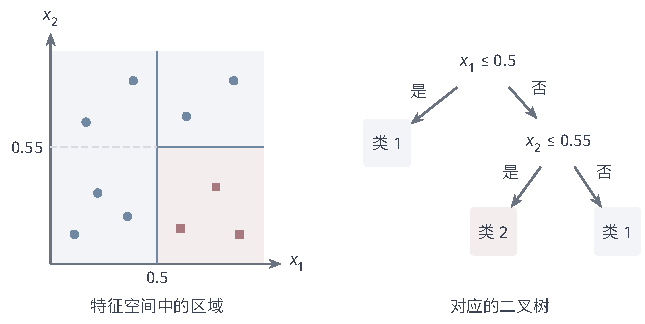
\includegraphics[width=109.241mm]{figures/04-classic-models/00-shared/tikz/classification-tree-partition/figure.pdf}
  \caption{二维分类的教学构造。左图为归一化特征空间$[0,1]^2$中的区域划分，圆点表示类1，方点表示类2；右图为产生同一划分的条件树。根节点检查$x_1\leq0.5$，仅在其“否”分支上继续检查$x_2\leq0.55$。点的位置与分裂阈值均为人为设定，不代表真实数据实验。}
  \label{fig:classification-tree-partition}
\end{figure}

不同树算法的主要差异落在三个问题上：怎样评价一次分裂，允许什么样的分支结构，怎样控制树的大小。ID3提供了信息增益驱动的基本构造，C4.5扩展其评分和数据处理方式；CART则采用统一的二叉划分与子树选择框架，形成了另一条决策树研究路线。

\subsection{ID3}
\label{sec:classification-id3}

要决定先检查哪个特征，需要比较“检查前还分不清多少类别”和“检查后还分不清多少类别”。ID3（Iterative Dichotomiser 3）据此选择特征，再在各分支上重复同一过程。Quinlan在1986年的论文中将ID3追溯到Hunt等人的概念学习系统（Concept Learning System, CLS）：CLS向前考察若干层候选树，按测量与误分类代价选择测试；ID3则改用信息驱动的局部评价。这一变化把建树中的“先测什么”落实为当前节点上可计算的信息增益比较，优化范围限定在当前节点的候选测试。本节采用以离散特征、信息增益和不作后剪枝为设定的基本ID3\scite{quinlan1986trees}。

\subsubsection{模型结构}
\label{sec:classification-id3-structure}

在节点样本集$D$上，记$p_c(D)$为类别$c$的样本比例。\term{熵}（entropy）用一个数概括类别分布的不确定性：节点只含一类时为零，各类越均匀，熵越大。采用以2为底的对数，
\begin{equation}
  H(D)=-\sum_{c=1}^{C}p_c(D)\log_2 p_c(D),
  \label{eq:classification-entropy}
\end{equation}
其中约定$0\log_2 0=0$。对第$j$个离散特征，令$V_j$为其可能取值集合，$D_{j,v}=\{(\bm{x}_i,y_i)\in D:x_{i,j}=v\}$。该特征的\term{信息增益}（information gain）是分裂前后熵的减少量：
\begin{equation}
  \operatorname{Gain}(D,j)
  =H(D)-\sum_{v\in V_j}\frac{|D_{j,v}|}{|D|}H(D_{j,v}).
  \label{eq:classification-information-gain}
\end{equation}
空子集对求和的贡献定义为零。这里必须按子集大小加权，否则只有一个样本的小分支会与包含大部分样本的分支同样重要。

ID3用选中的特征建立一个内部节点，每个取值对应一个分支。叶节点保存到达该处的类别计数，并通常输出多数类；类别计数相同时使用预先固定的平局规则。这样得到的是分段常值分类器：同一叶区域内的所有输入具有相同预测。叶节点也可报告类别频率，但少量样本上的频率不应被直接理解为可靠的概率估计。

信息增益把分裂选择变成了可计算的局部比较，却有\term{多值偏差}（multivalued attribute bias）：取值很多的特征更容易把训练样本分成纯净的小组。若每条记录的编号都不同，用编号分裂会使所有子节点熵为零，增益达到$H(D)$，但对一个新编号几乎没有帮助。

\subsubsection{参数学习}
\label{sec:classification-id3-learning}

从根节点的$D_n$出发，算法计算所有可用特征的信息增益，选择最大者，再分别对其子集递归建树。离散特征已经按取值完全展开后，同一路径上不必再次使用它。若当前样本全部同类，就生成该类叶节点；若可用特征耗尽而标签仍不一致，就输出当前多数类。对训练时未出现的分支，可以保留以父节点多数类为输出的回退叶节点，使预测规则对新输入仍有定义。

每次选择只依据当前节点，因而这是\term{贪心搜索}（greedy search）：接受眼前收益最大的分裂，不回头枚举所有可能的整棵树。基本ID3不在建树后再作剪枝；限制最大深度、最小叶样本数或最小增益，属于另外加入的生长控制。尤其是“增益为零就停止”也会改变基本搜索行为：在异或关系中，单个特征的增益可能为零，而连续两次测试可以完全分开类别。停止规则既能减少无效分裂，也可能阻止发现特征交互。

\subsubsection{理论分析}

\paragraph{表达能力}
对有限取值特征，若允许一条路径检查全部$d$个特征、保留至多$\prod_j|V_j|$个叶，就能为每个取值组合单独指定类别。因此任意只依赖这些字段的确定性类别映射都在这个树类中；有标签噪声时，完整组合上的类别分布也可由相应叶的概率向量表示。逐层组合坐标条件使树能够表示高阶交互。例如四点异或只需先检查$x_1$、再在两个分支分别检查$x_2$，深度为2、叶数为4；一层树却只能按一个坐标分组，在等概率四点上至少有一半标签无法吻合。

一旦限制深度或合并叶，尚未区分的取值组合就必须共用预测。这个限制不能靠增加同类样本消除。同一份特征记录若对应不同标签，树也无法逐条区分，只能用类别分布或多数类概括该处的随机性。



\paragraph{收敛性}
离散特征在同一路径最多使用一次，因此树深度至多为$d$，递归必然停止。每层所有非空节点合计处理至多$n$条记录；按每个节点扫描剩余字段的直接实现，建树成本至多为$O(nd^2)$，不计显式列出未观测空分支的成本。有限树类中的最小训练错误一定存在，但逐节点最大化信息增益并不求解这个全局问题，不能把递归结束理解为找到了训练错误最小的树。

\paragraph{泛化性}
\begin{theorem}[ID3在有限离散输入下的期望分类风险界]
固定各字段的有限取值集合，令$V=\prod_j|V_j|$。完整输入组合上的确定性分类器至多有$C^V$个；ID3返回的树，无论如何选择分裂，都属于这个固定集合。由式\eqref{eq:regression-finite-class-deviation}，对$n$个独立同分布的训练样本，以至少$1-\delta$的概率，
\[
 R_{01}(\hat h)\leq\widehat R_{01}(\hat h)
       +\sqrt{\frac{V\log C+\log(2/\delta)}{2n}}.
\]
\end{theorem}

这个界直接覆盖由训练数据选出的树，却可能因输入组合太多而没有实用精度。限制树的规模可以缩小候选数；未预先限定的新类别取值或连续阈值不满足这里的有限输入假设。

\subsubsection{优化泛化能力}

若关注的不只是类别变纯，还包括分裂是否有足够的统计证据，可以采用Kass于1980年提出的\term{卡方自动交互检测}（chi-square automatic interaction detection, CHAID）。它对类别特征的取值与标签建立列联表，先合并类别分布差异不显著的取值，再比较各特征与响应的关联，按经过多重比较调整的检验结果选择分裂；证据不足时停止。剩下的取值组形成多路分支，适合把分群结果读作交叉分类，但连续变量通常需要先分组，分组方式会影响结果。检验显著性针对相应的关联原假设，树的预测误差还需另行评价\scite{kass1980chaid}。

\subsubsection{小结}
\label{sec:classification-id3-summary}

ID3把离散字段逐层组织为类别区域，用当前节点的信息增益决定下一次测试。取值很多的字段容易获得较高增益，训练噪声也可能被写成细小分支。关联检验提供了另一种控制生长的依据，C4.5则继续调整评分和数据处理；应区分测试能表达什么与搜索为何选择它。

\subsection{C4.5}
\label{sec:classification-c45}

ID3的基本构造已经能从离散特征递归建树，但前面用记录编号的例子说明，信息增益会偏爱把训练样本切得很细的特征。实际记录还常有连续测量值和缺失字段：不能为每个长度值都建立一条新分支，也不能遇到未知值就让预测失去定义。让树处理这些数据，需要同时调整测试评分、阈值选择与缺失记录的传递方式。

Quinlan在1993年的专著中给出了C4.5的完整程序体系。它沿用ID3的递归构造，用增益率抑制部分多值偏差，通过阈值测试处理连续变量，并以分数权重传递缺失记录；树长成以后，再用错误估计剪枝和规则提取控制结构。以下分别说明这些机制如何工作\scite{quinlan1993c45}。

\subsubsection{模型结构}
\label{sec:classification-c45-structure}

多值特征容易得到大增益，是因为它本身就把数据切得很细。C4.5用\term{信息增益率}（gain ratio）比较“类别信息的增加”与“产生这些分支所需的划分信息”。设测试$a$把$D$分成$D_1,\ldots,D_b$，令$q_v=|D_v|/|D|$，则
\begin{align}
  \operatorname{SplitInfo}(D,a)
  &=-\sum_{v=1}^{b}q_v\log_2 q_v,
  \label{eq:classification-split-information}\\
  \operatorname{GainRatio}(D,a)
  &=\frac{\operatorname{Gain}(D,a)}
  {\operatorname{SplitInfo}(D,a)}.
  \label{eq:classification-gain-ratio}
\end{align}
这里的信息增益仍按式\eqref{eq:classification-information-gain}计算，只把按特征取值划分替换为测试$a$的各个结果。分母为零意味着没有真正划分，不能参与比值比较。

小分母会改变增益率的排序：只分离少量样本的测试具有较小的划分信息，微小信息增益也可能得到较大比值。C4.5先计算候选的平均信息增益，再在增益不低于平均值的测试中比较增益率。这个启发式筛选限制依靠小分母取胜的候选，实际预测价值仍由独立验证评价。

\subsubsection{参数学习}
\label{sec:classification-c45-learning}

离散特征可以按取值作多路分裂；连续特征则使用$x_j\leq t$与$x_j>t$的二路测试。候选阈值来自排序后相邻不同取值之间，且分裂后必须满足最小子节点样本量等限制。连续特征在某次分裂后仍可在后代节点使用，因为同一数值轴上可能需要多个阈值。

C4.5各版本对阈值的评价略有区别。较早版本按增益率选择阈值；Quinlan在1996年的修订中先按信息增益选择连续特征的阈值，再扣除搜索阈值所需的描述长度代价，参与特征之间的增益筛选和增益率比较。若有$q$个候选切分位置，这项逐样本惩罚形如$\log_2 q/|D|$，用来抵消“可试阈值更多”带来的选择优势。算法~\ref{alg:classification-c45}突出这些版本共有的建树骨架，把阈值评价留在候选测试生成步骤中\scite{quinlan1996continuous}。

\begin{algorithm}[C4.5的递归生长与后剪枝]
  \label{alg:classification-c45}
  \begin{algorithmic}[1]
    \Require 节点样本$D$，可用特征集合$F$，停止及剪枝设置
    \Ensure 剪枝后的分类树
    \Function{Grow}{$D,F$}
      \If{$D$全部同类，或样本量不足，或$F$为空}
        \State \Return 以$D$中多数类为输出的叶节点
      \EndIf
      \State 生成各特征的有效测试，连续特征同时选择阈值
      \State 计算各测试的增益；缺失值按正文约定处理
      \If{没有有效测试，或最大增益不为正}
        \State \Return 以$D$中多数类为输出的叶节点
      \EndIf
      \State 求候选测试的平均增益$\bar g$
      \State 保留增益不低于$\bar g$且划分信息为正的测试
      \State 选择其中增益率最大的测试$a$，建立节点$T$
      \For{测试$a$的每个结果$v$}
        \State 得到相应的子集$D_v$及子问题的特征集合$F_v$
        \If{$D_v$为空}
          \State 将$D$的多数类叶节点接到分支$v$
        \Else
          \State 将$\Call{Grow}{D_v,F_v}$接到分支$v$
        \EndIf
      \EndFor
      \State \Return $T$
    \EndFunction
    \State $T\gets\Call{Grow}{D,F}$
    \State 自底向上比较子树与简化方案的悲观错误估计
    \State \Return 剪枝后的$T$
  \end{algorithmic}
\end{algorithm}

缺失值需要在评分和路由中保留不确定性。设测试$a$的已知样本总权重占当前节点的比例为$q_{\mathrm{known}}$，C4.5在已知样本上估计熵下降，再乘$q_{\mathrm{known}}$降低该测试的收益；划分信息也计入未知部分。选择测试后，缺失记录按已知样本进入各分支的比例作分数权重分配，后续熵、类别计数和多数类都使用这些权重。预测遇到缺失值时，也按分支权重综合子树输出。

树生长完成后，C4.5采用\term{悲观错误剪枝}（pessimistic error pruning）：训练误差倾向于低估新样本错误，因而以二项错误计数的上置信估计作修正，比较保留子树与折叠成多数类叶节点的估计错误数。若简化方案不更差，就可以删除该子树；完整实现还可考察用某个子树提升替代当前分支。置信设置控制剪枝强度，这一自适应建树后的估计用于启发式模型选择，整树的样本外错误仍通过验证或测试数据评价。

树也可以转成规则：每条根到叶路径的测试构成规则前件，叶类别作为后件，再尝试删除不必要条件并筛选规则。未经简化的路径规则继承树的区域划分；条件删除以后可能产生重叠，因此规则系统还必须规定冲突处理和默认预测。这种转换并非只把树的文字抄成一份无序清单。

\subsubsection{理论分析}

\paragraph{表达能力}
连续特征的单坐标阈值把每个叶区域限制为坐标区间的交，也就是轴对齐的矩形或更高维的长方体。几个这样的区域可以精确表达前面的分段教学规则，却不能用有限条轴对齐边界精确重现整条斜线。表示限制在于分区方向，增益率只改变选择哪次分裂。

这个差距可以随着树的规模减小。例如，设输入在$[0,1]^2$上均匀分布，真实类别由$x_2>x_1$决定。把$x_1$轴等分为$m$个宽度$1/m$的区间，在每个区间内以其中点作为$x_2$阈值，至多$2m$个叶就能形成阶梯边界。每个竖条内与目标不一致的面积为$1/(4m^2)$，合计为$1/(4m)$。因此，至多$2m$叶的候选族中存在一个标签不一致比例为$1/(4m)$的表示。缺失字段的输入则没有提供该坐标的真实值；若两个对象的已观测字段相同，仅依赖这些字段的候选无法区分它们。



\paragraph{收敛性}
对完整输入，合法分裂将节点中的样本分为至少两个非空子集，沿任一路径的样本数严格减少，故至多$n$个非空叶后生长结束。缺失记录按权重分流时，不能继续用这条整数计数证明；实现需明确最小有效样本量，并可用预定最大深度保证有限终止。剪枝对有限树作有限次替换，同样会结束。增益率与局部错误估计都不是整棵树训练目标的精确求解器，因此没有由这些步骤自动推出的全局最优收敛率。

\paragraph{泛化性}
\begin{theorem}[C4.5冻结候选树在独立验证下的期望风险界]
连续阈值由训练数据确定，缺失输入还可能混合多个分支，因而不能只数最终树上出现的阈值来控制训练偏差。可以先用生长数据生成$J$棵完整预测规则固定的候选树，再在独立的$m$个同分布验证样本上选择错误率最小的$\hat h$。条件于这些候选树，零一损失的Hoeffding界与并集界给出，以至少$1-\delta$的概率，
\[
 R_{01}(\hat h)\leq\min_{1\leq j\leq J}R_{01}(h_j)
            +2\sqrt{\frac{\log(2J/\delta)}{2m}}.
\]
\end{theorem}

前一项保留候选树本身的质量，后一项控制验证选择的误差。该结论适用于这一独立验证协议，不能替换为C4.5内部的悲观错误估计；反复读取同一验证集来生成新树也不满足冻结候选的条件。

\subsubsection{优化泛化能力}

来自不同抽样来源的记录，未必应有相同训练权重。C4.5之后的C5.0加入了样本权重、误分类代价和特征筛选等功能\scite{rulequest2017c50}。样本权重调节不同记录在拟合中的贡献，让树与规则的选择更接近所关注的数据分布。权重需要有相应的抽样或评价依据；任意放大某些记录的贡献并不保证降低总体风险。

\subsubsection{优化计算能力}

数据规模增加时，树或规则生成过程的时间与内存也会限制使用。C5.0在C4.5之后继续改进这些实现；RuleQuest提供商业版本和GPL源码版本，其公开实验报告了特定数据与硬件条件下的速度及内存改进\scite{rulequest2017c50}。比较时应固定数据、硬件和输出形式，因为生成树与生成规则集的开销可以不同。实现上的节省与误分类代价设置处理的是不同问题，需要分别记录资源消耗和分类错误。

\subsubsection{支持误分类代价不同的场景}

邮件过滤中，误拦一封正常邮件与漏放一封垃圾邮件可能具有不同代价。误分类代价把这种差异写入损失，使树与规则按所关心的错误代价评分和选择。这里扩展的是评价目标，预测仍使用相应的树或规则表示。

\subsubsection{小结}
\label{sec:classification-c45-summary}

C4.5在ID3式递归划分中补充分裂评分、连续阈值、缺失字段传递与后剪枝，并可把路径转成规则。它处理的困难不只是分裂后类别是否更纯，还包括记录怎样经过分支，以及长成的树应保留多少细节。

C5.0继续改善树与规则生成，并使训练能够考虑样本权重和误判代价。实现效率与实际决策中的错误成本因而进入选择，但仍应检查所用字段是否有意义、缺失值如何影响预测，以及最终条件能否被审阅。

\subsection{CART}
\label{sec:classification-cart}

另一种组织树的方法是把每次测试都限定成二选一，再统一研究大树中应保留哪些子树。\term{分类与回归树}（classification and regression trees, CART）采用这一框架；Breiman、Friedman、Olshen与Stone在1984年的专著中将树的构造、最优剪枝与统计性质放在同一体系中讨论。其中，代价复杂度剪枝把“怎样长出一棵大树”与“最终保留多大的子树”分开：生长阶段比较局部分裂，剪枝阶段形成候选子树序列，再用验证选择规模。因此，CART与ID3的区别不只是换一个不纯度指标，还涉及分支结构与整树选择。这里关注分类树；第\ref{sec:regression-cart}节的回归CART复用递归二分与代价复杂度剪枝，但按响应损失选择分裂并在叶内输出数值，本节则按类别不纯度或误分类代价分裂并输出类别标签或类别比例\scite{breiman1984cart}。

\subsubsection{模型结构}
\label{sec:classification-cart-structure}

CART分类树通常用\term{基尼不纯度}（Gini impurity）评价节点中类别的混杂程度：
\begin{equation}
  G(D)=1-\sum_{c=1}^{C}p_c(D)^2.
  \label{eq:classification-gini}
\end{equation}
它也等于从节点经验类别分布独立抽取两个标签时，两者不同的概率。对于产生左右子集$D_{\mathrm{L}}$和$D_{\mathrm{R}}$的测试$a$，比较
\begin{equation}
  \Delta G(D,a)=G(D)
  -\sum_{v\in\{\mathrm{L},\mathrm{R}\}}
  \frac{|D_v|}{|D|}G(D_v).
  \label{eq:classification-gini-decrease}
\end{equation}
基尼与熵都鼓励子节点变纯，但并不总给出相同的排序。基尼计算省去对数运算，整棵树的训练成本还包含阈值搜索与数据访问。

对连续特征，二分测试仍是阈值比较；对类别特征，测试可写成$x_j\in S$与$x_j\notin S$，其中$S$是部分取值组成的集合。寻找这个集合本身也是搜索问题，候选分组数随取值数增加，搜索成本需要计入建树预算。统一的二叉结构便于遍历和剪枝，但可能用多层测试表达一棵多路树的一次分裂。

\subsubsection{参数学习}
\label{sec:classification-cart-learning}

生长阶段反复选择基尼下降最大的有效二分测试，直到满足生长限制，得到一棵较大的树$T_0$。随后进行\term{代价复杂度剪枝}（cost-complexity pruning）：不再逐个比较局部增益，而是在$T_0$的候选子树中平衡拟合误差和叶节点数。令$L(T)$为树$T$的叶节点集合，$\hat c_\ell$为叶$\ell$的预测类别，定义
\begin{align}
  \widehat R(T)
  &=\frac{1}{n}\sum_{\ell\in L(T)}
    \sum_{(\bm{x}_i,y_i)\in D_\ell}
    \mathbb{1}\{y_i\neq\hat c_\ell\},
  \label{eq:classification-cart-empirical-risk}\\
  J_\alpha(T)&=\widehat R(T)+\alpha|L(T)|,
  \qquad \alpha\geq0.
  \label{eq:classification-cart-cost-complexity}
\end{align}
这里$\widehat R(T)$采用全训练集上的误分类比例，使不同子树的误差具有共同尺度。有些软件把叶不纯度的加权和作为剪枝代价；使用其参数时需要核对具体定义，再按该尺度解释$\alpha$。

剪枝路径可以由\term{最弱环节剪枝}（weakest-link pruning）生成。设内部节点$t$以下的子树为$T_t$，把它折叠成一个叶节点后，该区域对全训练集误差的贡献为$\widehat R(t)$；保留时贡献为$\widehat R(T_t)$。两种方案的代价相等时，
\begin{equation}
  \alpha_t=
  \frac{\widehat R(t)-\widehat R(T_t)}
       {|L(T_t)|-1}.
  \label{eq:classification-weakest-link}
\end{equation}
分子是折叠后增加的训练错误，分母是删去的叶数，因而$\alpha_t$衡量“每少保留一个叶节点要付出多少误差”。剪去最小$\alpha_t$对应的分支，再重新计算，就得到从大树到根叶节点的嵌套序列。若某些分支增加叶数却不降低误分类率，可先在$\alpha=0$时合并；临界值处可能有多个最优子树，按一致的最小子树约定处理平局。

对每个$\alpha$，上述序列包含相应的最优剪枝子树，最优性范围限定为给定$T_0$的剪枝子树。实际需要用验证集或交叉验证选择$\alpha$；交叉验证时，在各训练折内独立生长和剪枝，再评价对应验证折。

预测还要规定主测试字段缺失时如何分支。CART的\term{替代分裂}（surrogate split）寻找其他特征测试，按它们复现主分裂结果的程度选择替代；类别权重和误分类代价也可以改变生长与叶预测。具体实现采用哪些机制，需要与数据处理方式一同检查。

\subsubsection{理论分析}
\label{sec:classification-cart-theory}

\paragraph{表达能力}
CART与完整输入上的C4.5共享单坐标阈值的矩形分区能力，前面$2m$个叶、错误率$1/(4m)$的斜线逼近也可由二叉树实现。有限离散输入上的任意取值映射同样可以逐次二分展开，但叶数必须足以区分所需组合。二叉与多路的区别主要影响树深和条件复用，并不使基尼评分获得一种新的边界形状。

测试全集还会留下独立于叶数的限制。若两个输入对全部允许测试都给出相同结果，无论树怎样增长，它们都会走到同一叶，必须得到相同类别。测试集合固定时，增加叶数只能细化已允许的测试组合；目标所需的阈值或特征不在测试集合中时，逼近差距仍然存在。



\paragraph{收敛性}
在无缺失、每次产生两个非空子节点的设定下，生长至多产生$n$个非空叶。成本复杂度剪枝从这棵有限大树出发，每次减少内部节点，剪枝路径也有限。对固定叶数上限和有限测试集，全局最优树存在；但贪心生长不保证找到它。剪枝的最优性只针对给定大树的子树，不能扩展为所有可构造树的最优性。

\paragraph{泛化性}
节点类别变纯，是当前训练子集上的变化；要控制整棵树在新样本上的错误，还要把选测试、选结构和选叶标签造成的选择范围计入。先考虑一个明确受限的版本：输入没有缺失，抽样前给定有限测试集合，并限制最多保留多少个叶节点。
\begin{theorem}[CART在固定测试集与叶数约束下的期望分类风险界]
  \label{thm:classification-tree-risk}
  设训练样本独立同分布，类别数为$C\geq2$。抽样前固定$Q\geq1$个二值测试和叶数上限$L\geq1$；候选类$\mathcal T_{Q,L}$包含用这些测试构造、至多$L$个叶、各叶输出一个类别的所有二叉树。令
  \[
    u_{\mathrm T}=
      \sqrt{\frac{\log(2L/\delta)
        +(L-1)\log(4Q)+L\log C}{2n}},
       \qquad0<\delta<1.
  \]
  CART学习器通过生长与剪枝返回$\hat T\in\mathcal T_{Q,L}$。至少以$1-\delta$的概率，
  \[
    R_{01}(\hat T)
      \leq\widehat R(\hat T)+u_{\mathrm T}.
  \]
  在同一事件上，若
  $e_{\mathrm{opt}}=\widehat R(\hat T)
      -\min_{T\in\mathcal T_{Q,L}}\widehat R(T)$，则
  \[
    R_{01}(\hat T)-R^\ast
      \leq\inf_{T\in\mathcal T_{Q,L}}R_{01}(T)-R^\ast
            +2u_{\mathrm T}+e_{\mathrm{opt}}.
  \]
\end{theorem}
\begin{proof}
  有$\ell$个叶的有序满二叉树形状数为第$\ell-1$个Catalan数，至多$4^{\ell-1}$。每个内部节点有$Q$种测试，每个叶有$C$种输出，所以
  \[
    |\mathcal T_{Q,L}|
       \leq\sum_{\ell=1}^L4^{\ell-1}Q^{\ell-1}C^\ell
       \leq L(4Q)^{L-1}C^L.
  \]
  零一损失位于$[0,1]$，对这个预定有限类应用式\eqref{eq:regression-finite-class-deviation}的一致偏差界，便得$u_{\mathrm T}$。该事件同时覆盖全部候选树，因此也覆盖依训练数据选出的$\hat T$。用它先比较$R_{01}(\hat T)$与$\widehat R(\hat T)$，再加上$e_{\mathrm{opt}}$并与任意候选树比较，最后把候选树的经验风险换回期望风险，即得第二个结论。
\end{proof}

这里不要求CART找到所有树中的经验最优解；贪心生长和给定大树内的最优剪枝，未必使$e_{\mathrm{opt}}$为零。第一个界对任意返回的受限树成立，第二个界则保留它与候选类经验最优者的搜索差距。叶数增多可能减小逼近差距，却同时增大抽样误差项。

在完整的有限类别输入上，ID3与C4.5的多路测试也可以展开为若干二值测试；若测试全集和叶数上限预先固定，展开后的树满足同一个结论。通常实现从训练数值中挑选连续阈值，或对缺失输入混合分支预测，这些情形没有自动满足上述有限类假设。尤其不能在建树之后，把实际考察过的测试数当作预定的$Q$。若对独立验证集上的一条预先生成剪枝路径选择子树，可以条件于生长数据，再按候选子树数控制验证选择；其风险依据来自验证抽样，而不是节点不纯度本身。

\subsubsection{优化表达能力}

常数叶用一个概率向量概括区域中的全部输入；若同一区域内的概率仍随特征变化，可以保留树的划分，改变叶节点如何预测。\term{逻辑模型树}（logistic model tree, LMT）在每个叶区域内使用Logistic回归，即用特征的线性得分表示类别对数几率，再转成类别概率。这样，树负责不同区域之间的结构变化，叶模型负责区域内部随特征变化的概率。Landwehr、Hall与Frank的2005年期刊论文基于其2003年会议工作，结合C4.5分裂与CART剪枝形成树结构，并通过LogitBoost逐步拟合逻辑模型。在后代节点继续细化祖先模型，可以避免每个小叶都从零估计全部系数\scite{landwehr2005lmt}。

例如在二分类叶区域$\ell$内，LMT可输出
\begin{equation}
  \hat p_\ell(y=1\mid\bm{x})
  =\frac{1}{1+\exp[-(\bm{w}_\ell^\top\bm{x}+b_\ell)]},
  \label{eq:classification-lmt-leaf}
\end{equation}
其中$\bm{w}_\ell\in\mathbb{R}^d$和$b_\ell\in\mathbb{R}$是叶模型的系数。概率在单个叶区域内部平滑变化，但跨越不同叶的边界时仍可能跳变，也不自动具有良好的校准性质。模型拟合、迭代次数选择和树剪枝共同增加训练成本，解释时也要同时阅读路径条件与叶模型系数。
LMT能精确表达“各叶区域内对数几率分别为仿射函数”的后验，只要树能够形成这些区域。普通常值叶只能用一个概率概括叶内全部输入；LMT可以保留其中的线性变化，却仍不能在具有非零长度的连续输入区间内精确表达$x^2$这样的对数几率。进一步划分区域能够改善逼近，不能免除叶数与样本覆盖的限制。

\subsubsection{优化泛化能力}

信息增益和基尼下降还面临另一种偏差：候选切分越多，越容易偶然找到一个高分切分。\term{条件推断树}（conditional inference tree, CTree）把“选哪个特征”与“在该特征上怎样切分”分开。Hothorn、Hornik与Zeileis在2006年的框架中用条件置换分布评价特征与响应的关联：先检验当前节点中所有特征均与响应无关联的全局原假设；不能拒绝时停止，否则选择检验证据最强的特征，再为它寻找二分位置。通过同一检验尺度和多重检验控制，可以缓解不同取值数目带来的选择偏差\scite{hothorn2006ctree}。

CTree的置换检验依赖原假设下的可交换性，渐近近似的精度也受样本量影响。检验控制当前节点是否继续分裂，全树的预测质量仍应在独立数据上评价。

检验驱动的生长也有搜索边界：四点异或在两层树中可被精确表示，但根节点的每个单坐标都与标签独立，单变量检验可能阻止继续分裂。检验决定当前节点是否继续搜索，并不改变候选树本来能够表示的关系。

\subsubsection{小结}
\label{sec:classification-cart-summary}

把叶节点多数类换成数值均值，把分类不纯度换成平方误差，就得到平方损失下的回归树构造；不需要另换一种树的表示。多个树怎样组合，见第\ref{chap:ensemble-learning}章。

CART把二叉分裂的局部选择与整树规模的验证选择分开。条件推断树采用另一种分裂依据，先比较特征与类别的关联，再确定切分位置；这种选择针对候选切分数影响评分的问题。

若常数叶遗漏区域内部的概率变化，逻辑模型树可以在叶内使用特征得分，并结合C4.5分裂与CART剪枝组织区域。代价是还要拟合和选择叶模型，解释时同时阅读路径与系数。分裂选择、树的规模和叶内预测各处理不同困难，类别不平衡、缺失字段与误判代价也须在对应机制中处理。

\subsection{规则分类与RIPPER}
\label{sec:classification-rules}
\label{sec:classification-ripper}

一棵树把全部输入组织成从根出发的路径，规则列表则可以直接列出若干足以作出类别判断的条件。例如，目标类若由几个分离的小区域组成，我们可以分别为这些区域学习短规则，而不要求它们共享同一个根测试。规则简化后还可能重叠，因而需要约定命中多条规则时怎样预测。第\ref{sec:classic-overview-tree-rules}节已介绍这种表示差别；这里采用有序规则，按首次命中的结论判类，没有命中时使用默认类。

逐条学习规则时，一个直接困难是：为了覆盖少量例外，不断增加条件会产生庞大的规则集；过早删去条件，又可能丢失有用的局部结构。早期的AQ系列探索了从样本归纳条件规则的路线，后来的规则学习把覆盖策略与误差控制结合起来。Fürnkranz与Widmer在1994年提出\term{增量减错剪枝}（incremental reduced error pruning, IREP），将单条规则的增长和立即剪枝嵌入逐条学习过程，以避免先生成庞大规则集再统一简化的开销\scite{furnkranz1994irep}。

Cohen在1995年改进IREP的剪枝评分和停止准则，并加入整组规则的反复优化，形成RIPPER（Repeated Incremental Pruning to Produce Error Reduction）。RIPPER通过规则增长、留出剪枝、顺序覆盖和整组优化，在长度、覆盖范围与错误之间实施启发式搜索。下面分解这些步骤\scite{cohen1995ripper}。

\subsubsection{模型结构}
\label{sec:classification-ripper-structure}

RIPPER输出有序规则以及一个默认类别$c_0$。第$r$条规则的前件可写为
\begin{equation}
  a_r(\bm{x})=\bigwedge_{j=1}^{m_r}b_{r,j}(\bm{x}),
  \qquad a_r(\bm{x})\Longrightarrow y=c_r,
  \label{eq:classification-rule-form}
\end{equation}
其中$b_{r,j}$是一个返回真或假的测试，$m_r$为该规则的条件数。例如，$x_1>60$与$x_2=\text{是}$可以组成一个合取，但每个测试的业务含义必须由特征定义决定。规则\term{覆盖}（cover）样本，指样本满足其前件，与样本真实标签是否等于后件无关。

若规则数为$s$，预测时寻找最小的$r\in\{1,\ldots,s\}$使$a_r(\bm{x})$成立，输出$c_r$；不存在这样的$r$时输出$c_0$。二分类中，可以为目标类学习若干规则，把另一类作为默认类。多分类时，经典RIPPER通常按类别出现频率由低到高学习，逐次区分当前类与尚待区分的其他类，把最常见类放在默认位置。这种类别排序有助于为少数类显式生成规则，但不构成少数类召回率的保证。

\subsubsection{参数学习}
\label{sec:classification-ripper-learning}

RIPPER采用\term{顺序覆盖}（sequential covering），这个名字描述了规则逐条“占领地盘”的过程：每次只在还没有被任何规则覆盖的样本上学习一条规则，把它加到有序列表的末尾，然后把它命中的样本从工作集中拿走，再对剩下的样本学习下一条；如此反复，直到没有目标类样本剩下。需要强调的是，被一条规则误覆盖的负例虽然从“找下一条规则”的工作集中移除，但在给整组规则打分时仍然计入，因此一条乱覆盖负例的规则不会因为样本被移走就逃避惩罚。设当前目标类别为$c_+$，属于该类的记录称为正例，其余为负例。保留原始二类训练集$D^{(0)}$用于整体评分，另用$U$表示不断缩小的覆盖工作集。从$U$移除的误覆盖负例仍保留在$D^{(0)}$中，并计入整体错误。

学习单条规则时，先分层随机划分增长集与剪枝集，经典设置约为$2:1$。增长从空前件开始，空前件覆盖所有样本；每次添加一个测试，使前件更严格、覆盖范围更小。测试可直接使用连续特征的阈值，无须一律在训练前离散化。Cohen的实现对缺失特征采用保守约定：涉及该特征的测试在缺失记录上不成立，因此规则需要其他已知字段来覆盖这些记录。

增长时使用源自FOIL（First Order Inductive Learner）的信息增益评分。设加入条件前覆盖$p_0$个正例、$q_0$个负例，加入后覆盖$p_1$个正例、$q_1$个负例，其中$q$不表示全章的样本量$n$。在命题规则设定下，评分为
\begin{equation}
  g=p_1\left(
  \log_2\frac{p_1}{p_1+q_1}
  -\log_2\frac{p_0}{p_0+q_0}
  \right).
  \label{eq:classification-foil-gain}
\end{equation}
括号比较加入条件前后的正例纯度，外面的$p_1$避免只看纯度而忽略保留下来的正例数。候选条件必须保留正例并满足覆盖量等实现约束；增长通常持续到不再覆盖增长集负例，或没有可接受的改进条件。噪声样本可能使负例始终被覆盖，此时由可接受条件和覆盖约束结束增长。

剪枝则允许把规则末端的一串条件一起删掉，也就是比较增长过程中得到的各个前缀，而非只尝试删去一个条件。若某个前缀在剪枝集覆盖$p$个正例、$q$个负例，RIPPER的基本评分是
\begin{equation}
  v=\frac{p-q}{p+q},\qquad p+q>0.
  \label{eq:classification-ripper-pruning}
\end{equation}
在分母为正时，它与覆盖样本中的正确率$p/(p+q)$给出相同排序。剪枝选择评分最好的可接受前缀，平局可偏向较短者；覆盖不到剪枝样本时，分数未定义，需执行预先规定的回退或拒绝规则。这一评分改变了原IREP对规则的偏好，尤其避免单凭覆盖大量样本而认可纯度不足的条件。

单条规则看起来合理，也可能使整组规则过于复杂。\term{最小描述长度}（minimum description length, MDL）把这种取舍表达为：用多少比特写下规则，再用多少比特说明规则预测错了哪些训练标签。记有序规则集为$\mathcal{R}$，总描述长度可概括为
\begin{equation}
  L_{\mathrm{total}}(\mathcal{R};D^{(0)})
  =L_{\mathrm{rules}}(\mathcal{R})
   +L_{\mathrm{errors}}(D^{(0)}\mid\mathcal{R}).
  \label{eq:classification-rule-description-length}
\end{equation}
第二项按完整规则集及默认类计算，因而仍包含误覆盖记录。Cohen的实验允许总长度暂时超过此前的最小值，但超过64比特就停止增加规则，再从后向前删除会增加总长度的规则。64比特是该实现允许暂时增加描述长度的预算；规则增加后统一按总长度检查停止和删除。

算法~\ref{alg:classification-ripper}给出二类子问题的主要流程。伪代码中的增长和剪枝采用前述评分，描述长度的编码细节由具体实现确定；多分类时在外层加入类别排序与默认类约定。

\begin{algorithm}[RIPPER的覆盖学习与规则优化]
  \label{alg:classification-ripper}
  \begin{algorithmic}[1]
    \Require 二类样本$D^{(0)}$，目标类$c_+$，优化轮数$b$
    \Ensure 有序规则集$\mathcal{R}$及默认负类
    \State $\mathcal{R}\gets()$
    \Function{Extend}{$\mathcal{R},D^{(0)}$}
      \State $U\gets D^{(0)}$中未被$\mathcal{R}$覆盖的样本
      \State $L_{\min}\gets L_{\mathrm{total}}(\mathcal{R};D^{(0)})$
      \While{$U$中仍有正例}
        \State 将$U$分层随机划为增长集$G$和剪枝集$P$
        \State 从空前件增长规则$a$，按式\eqref{eq:classification-foil-gain}添加条件
        \State 在$P$上按式\eqref{eq:classification-ripper-pruning}选择$a$的前缀
        \If{无可接受规则，或$a$不覆盖$U$中的任何正例}
          \State \textbf{停止本轮覆盖学习}
        \EndIf
        \State 把$a\Longrightarrow c_+$追加到$\mathcal{R}$
        \State $L\gets L_{\mathrm{total}}(\mathcal{R};D^{(0)})$
        \State $L_{\min}\gets\min(L_{\min},L)$
        \If{$L>L_{\min}+64$}
          \State \textbf{停止本轮覆盖学习}
        \EndIf
        \State 从$U$移除被$a$覆盖的全部样本，包括正例和负例
      \EndWhile
      \State 从后向前删除能使总描述长度降低的规则
      \State \Return $\mathcal{R}$
    \EndFunction
    \State $\mathcal{R}\gets\Call{Extend}{\mathcal{R},D^{(0)}}$
    \For{$t=1,\ldots,b$}
      \For{按顺序考察$\mathcal{R}$中的每条规则}
        \State 从空前件生成替代规则，从原前件生成修订规则
        \State 剪枝候选规则时，评价完整规则集在剪枝集上的错误
        \State 用总描述长度在原规则、替代规则、修订规则之间选择
      \EndFor
      \State $\mathcal{R}\gets\Call{Extend}{\mathcal{R},D^{(0)}}$
    \EndFor
    \State \Return $\mathcal{R}$，无规则匹配时预测负类
  \end{algorithmic}
\end{algorithm}

优化阶段是在整组规则的上下文中改写单条规则。替代规则从空前件重新增长，修订规则在原前件上继续添加条件；对候选规则的剪枝不只看它自身的纯度，还看替换后完整有序规则集的错误。随后用MDL选择保留原规则还是采用候选，必要时重新进行规则删除和剩余正例的覆盖学习。原论文把一次优化称为RIPPER，重复两次称为RIPPER2；优化次数规定搜索预算，最终返回已搜索候选中的选定规则集。

\paragraph{搜索能保证到哪里}
\label{sec:classification-ripper-theory}
规则数量和条件长度决定能拼合哪些区域，当前增长、剪枝与替换策略决定实际访问哪些候选。每条有效规则至少覆盖一个尚未移除的正例，再规定有限的条件集合、规则长度和优化轮数，便可保证搜索结束；这不意味着找到了所有规则列表中的最小训练错误或最短描述。MDL与留出剪枝都是当前搜索中的选择依据，最后仍需在独立数据上评价整组有序规则。

\subsubsection{无序规则的组合}

有序规则按首次命中决定输出，排在前面的规则会遮住后面的匹配。Clark与Boswell在1991年对CN2规则学习的改进中研究了无序规则：针对类别分别生成条件，允许多个规则共同参与预测。有序规则以首次命中解决冲突；无序规则则需要组合匹配规则的类别分布或投票权重。无序表示减少了对单一顺序的依赖，却把解释负担转移到重叠和冲突处理上，因此规则学习和预测时的聚合约定需要配套选择\scite{clark1991cn2}。
无序版本改变了重叠区域中的输出组合，不能只按有序列表理解。减少顺序依赖也不意味着预测无需约定：冲突规则怎样合并、没有规则命中时怎样回退，都属于完整的分类器。

\subsubsection{CN2的束搜索}

RIPPER增长一条规则时沿当前条件链继续搜索；若希望同时保留几条条件链，可以比较另一种规则搜索策略。Clark与Niblett在1989年提出的CN2采用这种做法，是另一条直接规则学习路线。它结合AQ的规则覆盖思想与类似ID3的纯度评价，用\term{束搜索}（beam search）寻找条件合取：每轮扩展已有候选，只保留评分最好的$b$个候选继续搜索，其中$b$为束宽。

束宽大于1时，相较于每轮只保留一条条件链的贪心搜索，束搜索可以评价更多候选，也有机会继续探索另一条暂时评分较低的路径。相较于不截断、把全部扩展都保留下来的穷举，限制束宽又能减少后续需要扩展的候选数。这里的“增加计算”与“节省计算”使用了不同的比较基准。

例如，构造一个最多增长3步的搜索，每条候选链在每一步都恰有4个可扩展条件，且不合并重复候选。单链贪心每层评价4个候选，共$4+4+4=12$个；束宽为2时，第一层评价4个并保留2个，后两层各评价8个，共$4+8+8=20$个；不截断时则评价$4+16+64=84$个。这个例子只比较指定搜索树中的候选评价次数，不代表CN2在所有任务上的运行时间比例。

候选截断仍可能丢弃通向最优规则的条件链，因此束搜索不提供全局最优保证。CN2还用显著性筛选限制偶然形成的纯净小区域\scite{clark1989cn2}。

在相同条件全集、前件长度和列表规模下，有序CN2与RIPPER拥有相同的规则表示能力。束宽增加的是可能找到好规则的搜索机会，不新增条件本身无法表达的关系。

\subsection{模型对比与总结}
\label{sec:classification-trees-comparison}
\label{sec:classification-rules-comparison}

表~\ref{tab:classification-tree-comparison}比较局部分裂与整树规模怎样确定。输入包含连续值或缺失字段时，需要检查测试和分支处理；最终条件要供人审阅时，树深、规则数与冲突处理同样影响选择。

ID3、C4.5与CART共享逐层测试的表示，但没有使用同一套搜索准则。C4.5沿用ID3式构造，调整多值特征评分，并补充连续阈值、缺失记录传递与后剪枝。CART把每次分裂统一为二分，再通过代价复杂度路径选择子树。多路测试可以展开成若干二值测试，却可能需要更多节点；因此“二叉”与“多叉”的名称不能直接决定哪个候选树更简洁。输入处理、分裂选择和整树规模都需要在相同任务下比较。

\begin{table}[htbp]
  \centering
  \small
  \begin{tabularx}{\linewidth}{@{}l*{3}{>{\RaggedRight\arraybackslash}X}@{}}
    \toprule
    方法 & 分裂评分 & 基本分支形式 & 规模控制 \\
    \midrule
    ID3 & 信息增益 & 离散取值多路分裂 & 基本版本无后剪枝 \\
    C4.5 & 增益筛选与增益率 & 离散多路、连续阈值二分 & 悲观错误估计剪枝 \\
    CART & 基尼不纯度下降 & 统一二叉分裂 & 代价复杂度路径及验证选择 \\
    \bottomrule
  \end{tabularx}
  \caption{三种决策树在基本分类设定下的比较。输入支持和停止细节随实现版本变化。}
  \label{tab:classification-tree-comparison}
\end{table}

若尚不清楚复杂条件是否必要，可以先建立只依赖一个字段的基线。Holte在1993年研究的\term{单特征规则}（one rule, OneR）为每个字段建立“取值到多数类”的映射，再选择训练错误较少的字段；“one”指一个字段，通常仍有多条取值规则。它便于检查单字段能够解释多少差异，却不能使用不同字段的交互\scite{holte1993oner}。

需要按几个离散字段直接查询类别时，可以采用\term{决策表}（decision table），把所选字段的取值组合作为键，同键记录共用一个预测。Kohavi在1995年研究了用验证误差选择字段子集的办法。查表减少了逐条匹配条件的工作，但字段组合容易稀疏，连续值的分箱和未见组合的回退都需要另行规定\scite{kohavi1995decisiontable}。

当字段取值有限、允许使用全部取值组合且不限制结构规模时，树、规则列表和决策表都能为每个组合指定类别。它们的主要差异在于怎样组织和搜索这些条件：树复用共同的测试前缀，规则可以为不同局部区域采用不同条件顺序，决策表统一使用一组字段作为键。OneR则把全部判断限制在单个字段，不能表达跨字段交互；它适合检验复杂组合是否确有必要。

结构受限或组合未被样本覆盖时，这些表示才会显出不同取舍。树的深度限制会把一些输入留在同一叶内；规则列表需要处理覆盖、顺序与默认类；决策表需要为稀疏和未见键规定回退。应据此比较独立验证误差、条件数量与预测成本，并把条件能否被审阅作为实际约束。

\section{基于概率的分类}
\label{sec:classification-probability}

第\ref{sec:classic-overview-probabilistic}节已区分直接建立条件类别概率与先描述类条件输入分布的两条路线。本节分别用Logistic回归、朴素贝叶斯和GDA说明参数估计、类别决策与概率检验。沿用训练集$D_n$，类别数为$C$、类别索引为$c$；$p$按观测类型表示概率质量函数或概率密度。LDA的共享协方差推导见第\ref{sec:classification-lda}节，这里直接在一般高斯模型族中使用该结果。

\subsection{Logistic 回归}
\label{sec:classification-logistic}

感知机与SVM用得分的正负决定类别，但有些任务还需要知道判断有多大把握。例如，把一封普通邮件误判为垃圾邮件，可能比让一封垃圾邮件进入收件箱更难接受。此时我们希望调整判为垃圾邮件的门槛，并用类别概率计算两种决定各自的预期代价。分类得分可以另行校准为概率，也可以从一开始就建立概率模型。

LDA能计算类别概率，但先要拟合每类的输入分布，这要求对“每类的输入长什么样”作出较强假设。这里改为直接描述$\mathbb P(Y=1\mid\bm X=\bm x)$：只关心给定输入后属于正类的概率，对输入本身如何分布不作假设。我们仍用特征的加权和组织证据，不过线性得分可能小于$0$或大于$1$，不能直接作为概率——把一个可能取$-3$或$5$的数解释成“概率”显然没有意义。\term{Logistic回归}（logistic regression）用一个S形函数把整条实数轴上的得分“压缩”到$(0,1)$区间，从而转成正类概率；它不要求输入服从类条件高斯分布，所规定的是对数几率与特征的线性关系。本节采用标签$\{0,1\}$，名称中的“回归”指概率与特征关系的建模。

第\ref{sec:regression-glm}节把伯努利分布、logit链接与其他响应模型统一在广义线性模型中；本节复用这套条件概率结构，但进一步规定类别决策阈值与误判代价，并单独检查概率校准。

\subsubsection{模型结构}
\label{sec:classification-logistic-structure}

记$p(\bm{x})=\mathbb{P}(y=1\mid\bm{x})$。比值$p(\bm{x})/[1-p(\bm{x})]$称为\term{几率}（odds），衡量正类相对于负类的可能性。对它取对数得到\term{对数几率}（log-odds，也称logit），其取值可以覆盖整个实数轴，因而适合与线性得分连接：
\begin{equation}
  \label{eq:classification-logistic-logodds}
  \log\frac{p(\bm{x})}{1-p(\bm{x})}
  =\bm{w}^{\top}\bm{x}+b.
\end{equation}
其中$\bm{w}\in\mathbb{R}^{d}$是权重，$b\in\mathbb{R}$是偏置。令右侧为$z$，由$p/(1-p)=e^z$整理出$p=e^z/(1+e^z)$，便得到
\begin{equation}
  \label{eq:classification-logistic-sigmoid}
  p(\bm{x})=\sigma(\bm{w}^{\top}\bm{x}+b),
  \qquad
  \sigma(z)=\frac{1}{1+e^{-z}}.
\end{equation}
这个S形函数称为\term{Sigmoid函数}（sigmoid function），此处特指Logistic形式。它把任意有限得分转成严格介于零和一之间的数。Cox在1958年的二值序列回归研究是这一统计建模路线的经典文献\scite{cox1958binary}。

参数的解释落在对数几率尺度上：保持其他特征不变，$x_j$增加一个单位，正类几率乘以$e^{w_j}$。概率本身的变化还取决于原来的概率，因为
\[
  \frac{\partial p(\bm{x})}{\partial x_j}
  =w_jp(\bm{x})[1-p(\bm{x})].
\]
在其余特征固定时，$w_j$的符号表示模型中正类对数几率的变化方向，大小则依赖特征单位。例如$w_j=\log 2$、原概率为$1/2$时，该特征增加一单位将几率乘以2，概率变为$2/3$。这种条件关联的因果解释还需要有关数据生成与混杂的额外假设。

在两类误判代价相同时，以$p(\bm{x})\geq1/2$预测正类，边界就是$\bm{w}^{\top}\bm{x}+b=0$。若误报的代价为$a>0$、漏报为$r>0$，正确分类代价为零，则预测正类的条件是$a[1-p(\bm{x})]\leq rp(\bm{x})$，即阈值改为$a/(a+r)$。这一决策解释要求输入概率足够可靠；可靠程度应通过与实际频率的比较检验。

图\ref{fig:classification-logistic-probability}把概率阈值与得分阈值放在同一条曲线上比较。一般地，概率阈值$\tau\in(0,1)$对应得分阈值$\log[\tau/(1-\tau)]$。在图中的教学设定下，误报与漏报代价相等时取$\tau=0.5$；若改成$a=4$、$r=1$，则$\tau=0.8$，得分至少达到$\log4\approx1.386$才预测正类。曲线本身没有改变，改变的是把概率转成类别的规则。
\begin{figure}[htbp]
  \centering
  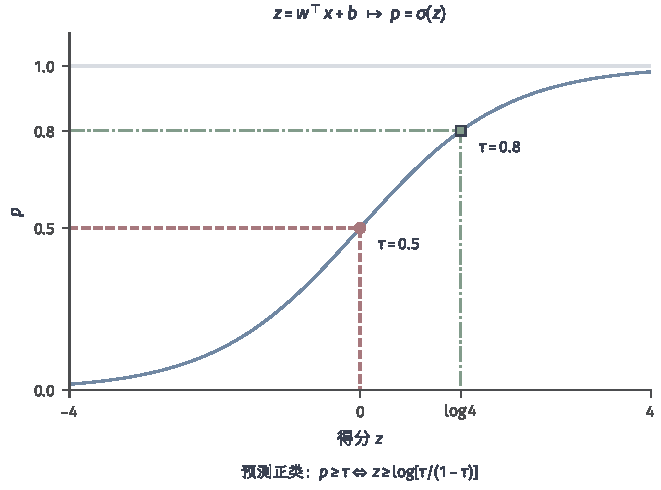
\includegraphics[width=105.412mm]{figures/04-classic-models/00-shared/matplotlib/classification-logistic-probability/figure.pdf}
  \caption{线性得分$z=\bm{w}^{\top}\bm{x}+b$经Logistic函数转为正类概率$p$。蓝色实线为$p=\sigma(z)$；红色虚线与圆点标出$(0,0.5)$，绿色点划线与方点标出$(\log4,0.8)$。两组辅助线分别连接概率阈值与对应的得分阈值，数值是教学构造，不表示训练或校准结果。}
  \label{fig:classification-logistic-probability}
\end{figure}

\subsubsection{参数学习}
\label{sec:classification-logistic-learning}

对独立样本，模型给出的标签概率为$p_i^{y_i}(1-p_i)^{1-y_i}$，其中$p_i=\sigma(\bm{w}^{\top}\bm{x}_i+b)$。\term{最大似然估计}（maximum likelihood estimation, MLE）选择使已观察标签最可能出现的参数。其条件对数似然为
\begin{equation}
  \label{eq:classification-logistic-likelihood}
  \ell(\bm{w},b)
  =\sum_{i=1}^{n}
  \bigl[y_i\log p_i+(1-y_i)\log(1-p_i)\bigr].
\end{equation}
最大化$\ell$等价于最小化负对数似然$L=-\ell$，也就是二分类\term{交叉熵损失}（cross-entropy loss）：给真实标签分配的概率越低，惩罚越大。令增广输入$\tilde{\bm{x}}_i=(\bm{x}_i^{\top},1)^{\top}$、参数$\bm{\beta}=(\bm{w}^{\top},b)^{\top}\in\mathbb{R}^{d+1}$，并记$z_i=\tilde{\bm{x}}_i^{\top}\bm{\beta}$，可写成
\begin{equation}
  \label{eq:classification-logistic-loss}
  L(\bm{\beta})
  =\sum_{i=1}^{n}\bigl[\log(1+e^{z_i})-y_i z_i\bigr].
\end{equation}
数值计算不宜先求极端概率再取对数，可用$\log(1+e^z)=\max\{0,z\}+\log(1+e^{-|z|})$避免指数溢出。

为确定更新方向，利用$\sigma'(z)=\sigma(z)[1-\sigma(z)]$求导。令$\tilde{\bm{X}}\in\mathbb{R}^{n\times(d+1)}$的第$i$行为$\tilde{\bm{x}}_i^{\top}$，$\bm{p}=(p_1,\ldots,p_n)^{\top}$、$\bm{y}=(y_1,\ldots,y_n)^{\top}$，则
\begin{equation}
  \label{eq:classification-logistic-derivatives}
  \begin{aligned}
    \nabla L(\bm{\beta})
      &=\tilde{\bm{X}}^{\top}(\bm{p}-\bm{y}),\\
    \nabla^2 L(\bm{\beta})
      &=\tilde{\bm{X}}^{\top}\bm{R}\tilde{\bm{X}},\\
    \bm{R}
      &=\operatorname{diag}\bigl(p_i(1-p_i)\bigr)_{i=1}^{n}.
  \end{aligned}
\end{equation}
梯度中的$p_i-y_i$是预测概率与观察标签的差。对任意$\bm{v}\in\mathbb{R}^{d+1}$，Hessian的二次型为
\[
  \bm{v}^{\top}\nabla^2L\,\bm{v}
  =\sum_{i=1}^{n}p_i(1-p_i)
    (\tilde{\bm{x}}_i^{\top}\bm{v})^2\geq0.
\]
所以负对数似然$L$是凸函数，而被最大化的$\ell$是凹函数。有限参数处的$p_i(1-p_i)>0$；若$\tilde{\bm{X}}$列满秩，$L$严格凸，否则可能存在不改变训练得分的平坦方向。这涉及\term{可识别性}（identifiability）：数据能否区分不同参数。即使严格凸，也只能保证有限极小点若存在便唯一，不能保证它一定存在。

例如，若存在$\bm{\beta}_0$使$(2y_i-1)\tilde{\bm{x}}_i^{\top}\bm{\beta}_0>0$对所有样本成立，沿$t\bm{\beta}_0$令$t\to\infty$，每项损失均趋于零，但任意有限$t$的损失仍大于零。完全分离的数据因此没有有限MLE；准完全分离也可能使部分参数发散。完整的存在性分析需要区分分离、准分离和重叠情形\scite{albert1984existence}。

实际训练常加入$\lambda\lVert\bm{w}\rVert_2^2/2$，其中$\lambda>0$。这个$L_2$惩罚抑制权重无限增大，也改善病态方向的数值条件。若两类均有样本，所有权重都受惩罚而偏置不受惩罚，所得二分类目标仍有唯一有限极小点；但若训练集只有一类，偏置仍可独自趋于无穷。若连偏置也作正的二次惩罚，则整个增广参数方向都受约束。使用$\lambda\lVert\bm{w}\rVert_1$可得到稀疏权重，但目标不再处处可微，需要适合非光滑目标的求解步骤。

求解器的选择取决于数据规模和存储成本。稠密数据的一轮完整梯度计算为$O(nd)$，构造Hessian约为$O(nd^2)$，直接分解又需要$O(d^3)$。若存储$d\times d$量级的Hessian过于昂贵，\term{有限内存拟牛顿法}（limited-memory BFGS, L-BFGS）只保留少量历史更新来近似二阶信息。大规模稀疏数据则可采用\term{随机梯度下降}（stochastic gradient descent, SGD），每次用一个样本或小批量近似完整梯度。样本数、稀疏程度和精度要求共同决定求解选择。

中小规模问题还可用牛顿法。把正则项加入梯度与Hessian后，每轮解$\bm H_t\bm d_t=-\nabla F(\bm\beta^{(t)})$，再以带阻尼的$\bm\beta^{(t+1)}=\bm\beta^{(t)}+\eta_t\bm d_t$更新；$F$是当前受惩罚目标。第\ref{sec:regression-glm}节已把同一步改写成IRLS：按当前概率产生工作响应和权重，再解加权最小二乘。这里沿用其计算，不把工作响应误当作固定的新标签。实现应解线性方程而不显式求逆，并检查目标变化、梯度与预算；极端概率、病态设计或过大的完整牛顿步都需要数值处理。

\paragraph{多类概率的表示与学习}

\label{sec:classification-logistic-softmax}

从垃圾邮件判断转到新闻主题分类，候选类别可以是体育、科技、文化等多个互斥主题。若分别训练“是否属于某主题”的二分类概率模型，它们的输出未必相加等于$1$；同一篇新闻可能在多个模型中都得到较高概率。我们需要一个共同描述类别竞争的模型。\term{Softmax回归}（softmax regression，也称multinomial logistic regression）为每类建立一个得分，再通过共同分母把这些得分转成和为一的概率向量。其表示约束是任意两类的对数概率比为线性函数。

\textbf{模型结构。}为每类引入$\bm{w}_c\in\mathbb{R}^{d}$和$b_c\in\mathbb{R}$，令$z_c(\bm{x})=\bm{w}_c^{\top}\bm{x}+b_c$。其后验模型为
\begin{equation}
  \label{eq:classification-softmax-model}
  p_c(\bm{x})
  =\mathbb{P}(y=c\mid\bm{x})
  =\frac{\exp z_c(\bm{x})}
         {\sum_{r=1}^{C}\exp z_r(\bm{x})}.
\end{equation}
指数保证概率为正，分母保证归一化；两类之间的分母相消，得到
\[
  \log\frac{p_c(\bm{x})}{p_r(\bm{x})}
  =(\bm{w}_c-\bm{w}_r)^{\top}\bm{x}+b_c-b_r.
\]
当$C=2$时，$p_1(\bm{x})=\sigma((\bm{w}_1-\bm{w}_2)^{\top}\bm{x}+b_1-b_2)$。把第1类视为正类、第2类视为负类，就回到二分类Logistic回归。

共同增加得分不会改变概率。更具体地，对任意$\bm{a}\in\mathbb{R}^{d}$和$t\in\mathbb{R}$，变换$\bm{w}_c\mapsto\bm{w}_c+\bm{a}$、$b_c\mapsto b_c+t$使每个指数项同乘$\exp(\bm{a}^{\top}\bm{x}+t)$，因而全部约掉。这是$d+1$维的参数冗余。选择第$C$类为\term{参考类}（reference class），就是把该类完整的增广参数固定为零：
\begin{equation}
  \label{eq:classification-softmax-reference}
  \begin{gathered}
    \bm{w}_C=\bm{0},\qquad b_C=0,\\
    \log\frac{p_c(\bm{x})}{p_C(\bm{x})}
    =\bm{w}_c^{\top}\bm{x}+b_c
    \quad(c<C).
  \end{gathered}
\end{equation}
参考类约束需同时固定权重与偏置。$\lambda\sum_c\lVert\bm{w}_c\rVert_2^2/2$只消除共同权重平移，还须例如令$\sum_c b_c=0$或惩罚全部偏置，才能锁定共同偏置平移。参数冗余消除后，设计矩阵的秩决定数据能否区分剩余方向，数据分离则影响有限解的存在性。

\textbf{参数学习。}现在$y_i\in\{1,\ldots,C\}$，记$p_{i,c}=p_c(\bm{x}_i)$，$\bm{\Theta}\in\mathbb{R}^{(d+1)\times C}$的第$c$列为$\bm{\beta}_c=(\bm{w}_c^{\top},b_c)^{\top}$。多类负对数似然是
\begin{equation}
  \label{eq:classification-softmax-loss}
  \begin{aligned}
    L(\bm{\Theta})
      &=-\sum_{i=1}^{n}\log p_{i,y_i}\\
      &=\sum_{i=1}^{n}\left[
        \log\sum_{c=1}^{C}e^{z_c(\bm{x}_i)}
        -z_{y_i}(\bm{x}_i)\right].
  \end{aligned}
\end{equation}
多分类同样可以通过迭代优化学习参数。为构造每轮更新，先对上述损失求导；以$\mathbb{1}\{\cdot\}$表示条件成立时为一、否则为零的指示函数，得到
\begin{equation}
  \label{eq:classification-softmax-gradient}
  \begin{aligned}
    \nabla_{\bm{w}_c}L
      &=\sum_{i=1}^{n}
        [p_{i,c}-\mathbb{1}\{y_i=c\}]\bm{x}_i,\\
    \frac{\partial L}{\partial b_c}
      &=\sum_{i=1}^{n}
        [p_{i,c}-\mathbb{1}\{y_i=c\}].
  \end{aligned}
\end{equation}
梯度仍由“预测概率减观察标签”组成。目标凸，但共同参数平移及秩亏可能带来平坦方向，分离数据也可能没有有限MLE。参考类约束消除表示冗余，正则化控制参数大小，两者的作用不同。

Softmax可用分块牛顿法、L-BFGS或小批量SGD优化，多类Hessian还包含类别间的耦合，不能简单把$C$个独立的二分类IRLS问题拼起来。求概率时应先减去$m(\bm{x})=\max_c z_c(\bm{x})$，用$e^{z_c-m}/\sum_r e^{z_r-m}$得到完全相同且更稳定的结果。普通稠密实现的一轮梯度计算约为$O(ndC)$。

预测可取$\hat y(\bm{x})=\argmax_c p_c(\bm{x})=\argmax_c z_c(\bm{x})$，并按固定类别次序处理平局。共同分母不改变得分排序，所以只需输出一个类别时，可以直接比较各类得分。

\paragraph{交叉熵在拟合什么}
\label{sec:classification-logistic-theory}
记真实类别后验为$\bm\eta(\bm x)$，预测概率向量为$\bm p(\bm x)$。固定输入时，预测交叉熵减去真实后验的熵为
\[
 -\sum_c\eta_c\log p_c+\sum_c\eta_c\log\eta_c
 =D_{\mathrm{KL}}(\bm\eta\Vert\bm p)\geq0.
\]
因此最理想的条件概率目标是真实后验；使用有限参数的Logistic或Softmax时，只能在所设定的对数几率关系中拟合它。若目标的对数几率需要平方或交互项，应改变输入特征，而不是只增加优化轮数。分类又只取最大概率的类别，所以概率拟合误差与分类错误是不同的评价对象。

\subsubsection{概率校准与温度缩放}

\label{sec:classification-probability-calibration}

需要用概率设定邮件拦截门槛时，还要检查报告的置信度能否对应实际频率。Softmax输出满足概率公理，却不自动满足\term{概率校准}（probability calibration）。例如，在报告某类概率约为$0.8$的一组样本中，该类的实际比例也应接近$0.8$。有限样本、模型失配、正则化和分布变化都可能破坏这种对应。这里检验的是报告概率与实际频率的联系，和按最大概率选择类别是不同的问题。

一种简洁的后处理是温度缩放（temperature scaling）：固定已训练得分$z_c(\bm x)$，只学习$T>0$，令$\tilde p_c(\bm x)=\exp(z_c/T)/\sum_r\exp(z_r/T)$。用未参与原模型拟合的校准记录最小化这组概率的负对数似然，就可估计温度；随后还要在另一份独立数据上评价。正温度不改变最高得分类别，却会改变概率的集中程度。Guo等在其研究的网络和数据上比较了这类方法；单一温度不能保证修复所有概率失配\scite{guo2017calibration}。

\subsubsection{层次Softmax、NCE与负采样}

\paragraph{降低大类别集的概率计算成本}
\label{sec:classification-softmax-hierarchical}

类别特别多时，平坦Softmax要在分母中累加全部类别的指数得分。\term{层次Softmax}（hierarchical softmax）改用树上路径概率的乘积表示一个类别的概率，把一次类别选择拆成沿路径进行的条件选择。这改变了概率的参数化方式，计算某个类别概率时可以沿相应路径展开；类别怎样组织成树，也就成为模型设计的一部分。若需要全部类别概率，计算负担仍然存在，沿路径计算一个类别的概率也不等于已经找到了最高概率类别\scite{goodfellow2016}。

用四个类别构造一个二叉树例子，可以分别看清归一化和搜索。把类别1、2放在根的左子树，类别3、4放在右子树。固定当前输入，设根节点向左的条件概率为$0.6$、向右为$0.4$；到达左子树以后，两片叶的条件概率为$0.5,0.5$；到达右子树以后，两片叶的条件概率为$0.99,0.01$。于是
\[
  \begin{aligned}
    p_1&=0.6\times0.5=0.3,&
    p_2&=0.6\times0.5=0.3,\\
    p_3&=0.4\times0.99=0.396,&
    p_4&=0.4\times0.01=0.004.
  \end{aligned}
\]
四类概率相加为一，因为每个内部节点都把到达它的概率质量完整分给两个孩子。内部节点可以各用一个Logistic模型给出两条分支的条件概率；一旦指定叶子，只需计算沿途节点，不必访问无关分支。在平衡二叉树中，路径长度约为$\log_2C$，不平衡树的路径则可能更长。给定类别树后，一条训练记录的真实类别就确定沿途的二元分支标签；训练时把这些节点的Logistic对数概率相加，沿路径求梯度并更新节点参数，无须访问无关分支。树的安排固定了哪些类别共享前面的判断，需要作为模型结构选择。

这个例子还表明，根处贪心选择较大的左支会错过概率最大的第3类。因此，计算指定类别的概率、找最高概率类别与输出全部类别概率，是三种不同的计算任务。

\paragraph{减少显式归一化的训练负担}
\label{sec:classification-softmax-noise-contrast}

当归一化分母需要对大量候选求和时，也可以改变概率估计所用的训练问题。\term{噪声对比估计}（noise-contrastive estimation, NCE）通过区分数据与人为噪声来估计模型，训练时回答一条记录来自数据还是人为噪声，模型参数也决定这项区分的得分。归一化常数可以与模型参数一起估计，避免每一步都对全部候选得分显式求和。它与层次Softmax改变的位置不同：前者改变估计问题，后者把类别概率分解到树上，不能把两者都当作原平坦Softmax公式的计算改写\scite{goodfellow2016}。

沿用新闻主题分类，可以把这一辅助任务写出来。固定输入$\bm x$，原任务的随机变量$Y$仍表示新闻主题，真实后验为$\eta_c(\bm x)$。现在对每一条真实记录$(\bm x,c^+)$，从已知、可抽样且可求值的噪声分布$q(c\mid\bm x)$独立抽取$k\geq1$个类别，组成噪声配对；这里取$q(c\mid\bm x)>0$覆盖全部候选类别。另引入二元来源标签$D$：真实配对的$D=1$，人为噪声配对的$D=0$。$D$回答配对怎样产生，$Y$回答新闻属于哪个主题，两者不是同一个类别变量。噪声抽样也可能恰好得到$c^+$，这不改变它的来源标签；若排除这种抽样结果，就必须相应改变噪声分布。

一条真实记录配$k$条噪声，意味着在混合记录中，两个来源的比例为$1:k$，而不是各占一半。固定同一个$\bm x$后，由贝叶斯公式，真实的来源后验为
\[
  \mathbb P(D=1\mid\bm x,c)
  =\frac{\eta_c(\bm x)}
    {\eta_c(\bm x)+kq(c\mid\bm x)}.
\]
这个式子把原主题后验接到了新增的来源区分任务上。NCE用原模型的非负质量替换未知的$\eta_c$。具体地，保留类别得分$z_{\theta,c}(\bm x)$，另外用可计算函数$\kappa_{\psi}(\bm x)$估计其对数归一化量，定义
\begin{equation}
  \label{eq:classification-nce-source-model}
  \begin{aligned}
    a_{\theta,\psi}(c\mid\bm x)
      &=\exp\{z_{\theta,c}(\bm x)-\kappa_{\psi}(\bm x)\},\\
    h_{\theta,\psi}(\bm x,c)
      &=\frac{a_{\theta,\psi}(c\mid\bm x)}
        {a_{\theta,\psi}(c\mid\bm x)+kq(c\mid\bm x)}\\
      &=\sigma\bigl(z_{\theta,c}(\bm x)-\kappa_{\psi}(\bm x)
                  -\log[kq(c\mid\bm x)]\bigr).
  \end{aligned}
\end{equation}
$\theta$控制原类别得分，$\psi$控制归一化量的函数表示；二者通过$h$共同影响来源预测。训练中$\kappa_{\psi}(\bm x)$不必已经等于$\log\sum_r e^{z_{\theta,r}(\bm x)}$，所以$a_{\theta,\psi}$暂时未必在类别上相加为一；但$h$始终是严格介于零和一之间的二元预测。条件模型的归一化量一般随$\bm x$变化，不能未经假设就用一个共享常数代替。所选$\kappa_{\psi}$的表示与求值也有成本，需要另行规定；若它不能表示所需的归一化函数，估计便会受到这项限制。

令第$i$条真实记录为$(\bm x_i,y_i)$，对应噪声类别为$c^-_{i,1},\ldots,c^-_{i,k}$。既然要提高真实配对来自数据的预测概率，同时提高噪声配对来自噪声的预测概率，每条记录的辅助对数目标就是
\begin{equation}
  \label{eq:classification-nce-objective}
  \begin{aligned}
    J_i^{\mathrm{NCE}}(\theta,\psi)
      &=\log h_{\theta,\psi}(\bm x_i,y_i)\\
      &\quad+\sum_{j=1}^{k}
        \log[1-h_{\theta,\psi}(\bm x_i,c^-_{i,j})].
  \end{aligned}
\end{equation}
对训练记录求和并最大化这个目标，就把原模型参数与归一化参数接入同一项来源分类训练。每次计算只访问真实类别和抽中的$k$个类别得分，无需在该步显式计算全类别指数和；噪声抽样、噪声概率与$\kappa_{\psi}$的计算成本仍需计入。

来源概率与主题概率的数值也不同。例如，三个主题使用均匀噪声，取$k=2$；若某主题的真实后验为$0.6$，则相应来源后验为$0.6/(0.6+2/3)\approx0.474$。因此不能把训练得到的$h$直接当作原主题后验。NCE的统计结论还依赖噪声支持、模型正确指定、归一化函数的可表示性、可识别性以及抽样和优化条件；上述构造没有证明有限样本下$a$已经精确归一化，也没有把辅助目标与原Softmax似然说成同一个目标。若预测接口要求完整的主题概率向量，仍需明确恢复或计算类别归一化，并另外检查校准。

\paragraph{减少每步训练的负例比较}
\label{sec:classification-softmax-negative-sampling}

若每次更新都比较全部其他类别，训练计算会随类别集增大。\term{负采样}（negative sampling）只对抽取的负例建立局部区分目标，减少这一步参与比较的对象。它通常改变原Softmax训练目标，因而应按实际采用的目标解释训练结果；需要类别概率时，也不能直接把局部区分得分当成前面归一化的概率向量\scite{goodfellow2016}。

继续使用一条真实配对与$k$条噪声配对，令$s_\theta(\bm x,c)$为可训练的配对得分。一种常见负采样目标为
\begin{equation}
  \label{eq:classification-negative-sampling-objective}
  \begin{aligned}
    J_i^{\mathrm{NEG}}(\theta)
      &=\log\sigma(s_\theta(\bm x_i,y_i))\\
      &\quad+\sum_{j=1}^{k}
        \log\sigma(-s_\theta(\bm x_i,c^-_{i,j})).
  \end{aligned}
\end{equation}
第一项提高真实配对的得分，第二项降低噪声配对的得分。两种方法都用少量配对训练二元区分，但上面的NCE把区分得分明确写成原模型对数质量减去$\log[kq(c\mid\bm x)]$；这个负采样目标的样本项只使用$s_\theta$，没有显式使用该噪声概率修正和归一化函数。噪声分布仍通过抽样影响训练结果，不能理解成负采样与$q$无关。若没有另外建立从$s_\theta$恢复类别概率的关系，$\sigma(s_\theta)$表示的仍是辅助区分预测，不是各主题相加为一的后验；也不能把该目标解释成仅从原Softmax分母删除未抽中的项。

\subsubsection{稀疏概率核模型：相关向量机}
\label{sec:classification-rvm}

核SVM用支持向量形成得分；若希望同时学习概率，并压缩预测时需要的基函数，可以采用Tipping的\term{相关向量机}（relevance vector machine, RVM）。它沿用Logistic概率，却把得分写成$g(\bm x)=\sum_{j=1}^m w_j\phi_j(\bm x)$；候选基函数通常取训练点为中心的核函数并加入常数项。每个系数分别有先验$w_j\sim\mathcal N(0,\alpha_j^{-1})$，其中$\alpha_j>0$是待学精度，即方差的倒数。精度大时，该基函数的系数受到更强收缩，而不是预先规定哪些样本必须成为支持向量\scite{tipping2001rvm}。

固定精度后，先以原伯努利似然乘这些高斯先验，最大化后验；这等价于最小化Logistic负对数似然加$\bm w^\top\bm A\bm w/2$，其中$\bm A=\operatorname{diag}(\alpha_1,\ldots,\alpha_m)$。牛顿或IRLS求得众数$\hat{\bm w}$后，RVM用众数附近的高斯近似来描述后验，这称为Laplace近似。令$\bm\Phi\in\mathbb R^{n\times m}$满足$\bm\Phi_{i,j}=\phi_j(\bm x_i)$，以$p_i=\sigma(g(\bm x_i))$记当前正类概率，并令$\bm B=\operatorname{diag}(p_i(1-p_i))_{i=1}^n$，则$m\times m$的近似协方差为
\[
  \bm\Sigma=(\bm\Phi^\top\bm B\bm\Phi+\bm A)^{-1}.
\]
原方法再依据近似边缘似然更新精度，例如使用固定点更新$\alpha_j\leftarrow(1-\alpha_j\bm\Sigma_{j,j})/\hat w_j^2$，并交替重算后验众数与协方差。数值上按阈值剔除受到强收缩的基函数，配合目标变化或迭代预算停止；分母过小等退化情况需要数值处理，精度学习也不保证全局最优。

最终保留的基函数及其系数构成稀疏预测器。若对近似后验积分，得到的是近似贝叶斯类别概率；只代入众数则是点估计预测，二者应区分。RVM改变了SVM的间隔准则和参数选择机制，有限精度只保证收缩，不保证系数恰为零；稀疏程度、计算收益与概率质量仍需验证。

\subsection{朴素贝叶斯}
\label{sec:classification-naive-bayes}

判断一封邮件是不是垃圾邮件，也可以换个问法：“如果它是垃圾邮件，有多大概率出现这些词？如果是正常邮件呢？”比较这两个问题的答案，再结合两类邮件各自的比例，就能反推它属于垃圾邮件的概率。如果以$d$个词是否出现作为二值特征，完整类条件分布就有$2^d$种输入组合；即使只选20个词，也已有一百多万种组合，很多组合在训练集中一次都没有出现。逐项估计它们的概率，需要远多于单个词频统计的数据，其中绝大部分组合的计数都会是零。

要打破这个组合爆炸，可以作一个简化假设：一旦知道了邮件类别，各个词是否出现就彼此无关。这并不要求现实中词与词真的独立——给定“这是垃圾邮件”之后，“免费”和“领取”仍可能一起出现——而是用一个乘积近似来换取可计算性。\term{朴素贝叶斯}（naive Bayes, NB）正是基于给定类别后各特征条件独立这一假设，把单个特征的概率相乘，得到输入的类条件概率。这样，无需等待整套词语组合反复出现，就能从各词的计数估计类别证据。简化也会遗漏词语依赖：例如给定邮件类别后，“免费”与“领取”仍可能共同出现得更多。模型用较少统计量换取可直接计算的估计，样本波动可能减小，依赖假设造成的偏差则仍会保留。

Maron在1961年关于自动索引的研究，是概率方法用于文档归类的早期工作之一。文档分类需要从大量词项中提取可累积的类别证据，这也成为朴素贝叶斯的一项典型用途\scite{maron1961indexing}。

\subsubsection{模型结构}
\label{sec:classification-naive-bayes-structure}

对一般特征向量，NB采用给定类别后的\term{条件独立}（conditional independence）假设：已知$y=c$后，一个特征的取值不再改变其他特征的分布。令$\pi_c=\mathbb{P}(y=c)$、$p_{j,c}(x_j)=p(x_j\mid y=c)$，模型写成
\begin{equation}
  \label{eq:classification-naive-bayes-model}
  \begin{aligned}
    q_c(\bm{x})&=\prod_{j=1}^{d}p_{j,c}(x_j),\\
    \mathbb{P}_{\mathrm{NB}}(y=c\mid\bm{x})
      &=\frac{\pi_c q_c(\bm{x})}
      {\sum_{r=1}^{C}\pi_r q_r(\bm{x})}.
  \end{aligned}
\end{equation}
记号$q_c$强调这是模型使用的乘积分布，未必等于真实类条件分布。条件独立不要求全部训练样本混在一起时特征仍独立，例如词项之间的总体相关性可能部分来自主题差异。

只需要分类时，各类共同的分母可以省略。为避免许多小概率连乘下溢，通常比较对数得分
\begin{equation}
  \label{eq:classification-naive-bayes-score}
  s_c(\bm{x})
  =\log\pi_c+\sum_{j=1}^{d}\log p_{j,c}(x_j),
  \qquad
  \hat y(\bm{x})=\argmax_c s_c(\bm{x}).
\end{equation}
这里$s_c$不是归一化的对数后验；需要概率时还须减去$\log\sum_r e^{s_r}$。零概率可使得分为负无穷，后面的平滑正是为未见事件保留概率质量。文档的多项式版本沿用相似得分，但它的独立性对象是词元位置，而非总长度固定后的各维计数，必须另外说明。

\subsubsection{参数学习}
\label{sec:classification-naive-bayes-learning}

令$n_c=\sum_i\mathbb{1}\{y_i=c\}$，类先验的MLE为$\hat\pi_c=n_c/n$。这是以训练样本的类别比例估计目标总体的比例，依赖抽样具有代表性；人为重采样改变类别比例，部署先验需要按抽样机制修正或另行估计。也可以使用有依据的外部类别比例；若希望保留对该比例的不确定性，并为训练中未见的类别保留概率质量，则可对类概率向量$\bm{\pi}=(\pi_1,\ldots,\pi_C)^{\top}$设置参数先验。以下对类别概率与各组类条件参数设置相互独立的先验，以便分别更新。

若使用正参数$\gamma_c$的Dirichlet参数先验，观察类别计数后的参数变为$\gamma_c+n_c$，相应后验均值为
\[
  \tilde\pi_c=\frac{n_c+\gamma_c}{n+\sum_r\gamma_r}.
\]
伪计数使未见类别仍有正概率；其总量控制先验相对于数据的影响。“类别先验$\pi_c$”属于样本生成模型，“对$\bm\pi$设置参数先验”描述估计它之前的不确定性，两者不能混同。Dirichlet分布的形式可参考\BookChapterRef{chap:random-variables}{卷二《数学准备：概率、因果与决策》的“随机变量”章}。

连续特征可采用\term{高斯朴素贝叶斯}（Gaussian naive Bayes），即$x_j\mid y=c\sim\mathcal{N}(\mu_{j,c},\sigma_{j,c}^{2})$，其中$\sigma_{j,c}^{2}>0$。当$n_c>0$且该特征的类内平方偏差和为正时，均值和方差的MLE为
\begin{equation}
  \label{eq:classification-naive-bayes-gaussian}
  \begin{aligned}
    \hat\mu_{j,c}
      &=\frac{1}{n_c}\sum_{i:y_i=c}x_{i,j},\\
    \hat\sigma_{j,c}^{2}
      &=\frac{1}{n_c}\sum_{i:y_i=c}
        (x_{i,j}-\hat\mu_{j,c})^2.
  \end{aligned}
\end{equation}
方差分母为$n_c$，不是无偏样本方差所用的$n_c-1$。在上述条件下，预测时将这些量代入一维高斯密度后相乘。若某类某特征恒定为$a$，固定$\mu_{j,c}=a$后，对数似然为$-n_c\log(2\pi\sigma_{j,c}^{2})/2$，随正方差趋于零而无界增大。因此，此时正方差参数域内没有有限MLE；式\eqref{eq:classification-naive-bayes-gaussian}给出的零值只是样本散度，不能代入普通高斯密度。设定有明确尺度的方差下限或加入先验后，得到的是相应的受约束或正则化估计；给密度任意“加一”不是离散概率的平滑对应物。

只关心某个词是否出现时，可用\term{伯努利朴素贝叶斯}（Bernoulli naive Bayes）。输入$x_{i,j}\in\{0,1\}$，令$n_{j,c}=\sum_{i:y_i=c}x_{i,j}$，则
\begin{equation}
  \label{eq:classification-naive-bayes-bernoulli}
  \begin{aligned}
    q_c(\bm{x})
      &=\prod_{j=1}^{d}
        \theta_{j,c}^{x_j}(1-\theta_{j,c})^{1-x_j},\\
    \hat\theta_{j,c}&=\frac{n_{j,c}}{n_c}.
  \end{aligned}
\end{equation}
$x_j=0$也通过词缺失概率提供证据，因此两种取值的项都参与得分；这里的MLE要求$n_c>0$。
为平滑这个二值事件，使用Beta分布作为$\theta_{j,c}$的先验，
两个正参数$\alpha_1,\alpha_0$分别对应出现与未出现。乘以似然后，
两项指数分别增加$n_{j,c}$和$n_c-n_{j,c}$，所以
\[
  \theta_{j,c}\mid D_n
  \sim\operatorname{Beta}
    (\alpha_1+n_{j,c},\,\alpha_0+n_c-n_{j,c}).
\]
其后验均值为$(n_{j,c}+\alpha_1)/(n_c+\alpha_1+\alpha_0)$；对称情形$\alpha_1=\alpha_0=\alpha$的分母是$n_c+2\alpha$。这同时平滑了出现和未出现两种事件。

若重复出现的次数也有意义，应使用\term{多项式朴素贝叶斯}（multinomial naive Bayes）。设固定词表有$d$个词项，$\bm{x}_i\in\mathbb{N}_0^d$记录一篇文档的词项计数，$m_i=\sum_jx_{i,j}$是该文档的总词元数。给定类别和$m_i$，假设每个词元位置独立地按$\bm{\theta}_c=(\theta_{1,c},\ldots,\theta_{d,c})^{\top}$抽取词项，其中$\sum_j\theta_{j,c}=1$。忽略顺序后，计数向量服从
\begin{equation}
  \label{eq:classification-naive-bayes-multinomial}
  \mathbb{P}(\bm{x}_i\mid y_i=c,m_i)
  =\frac{m_i!}{\prod_{j=1}^{d}x_{i,j}!}
    \prod_{j=1}^{d}\theta_{j,c}^{x_{i,j}}.
\end{equation}
因为计数总和已固定，各维计数并不独立。将它写成每维整数取值的独立类别分布，会改变模型和分母。McCallum与Nigam专门比较了伯努利和多项式这两种文档事件模型，明确区分“词是否出现”与“词出现多少次”\scite{mccallum1998event}。

标准文档分类通常进一步假设长度分布与类别无关，因而$\mathbb{P}(m_i\mid y_i=c)$在类别比较中约掉，此时给定长度后的类先验仍为$\pi_c$。若长度本身携带类别信息，则应保留并估计该项，使长度也参与后验计算。

令$t_{j,c}=\sum_{i:y_i=c}x_{i,j}$为第$c$类中词项$j$的总出现次数，$t_c=\sum_jt_{j,c}$为该类的总词元数。去掉与参数无关的组合系数后，类内对数似然为$\sum_jt_{j,c}\log\theta_{j,c}$。当$t_c>0$时，在$\sum_j\theta_{j,c}=1$约束下求极值，正计数坐标上的拉格朗日方程给出$t_{j,c}/\theta_{j,c}$为同一常数，零计数坐标取零；求和确定常数为$t_c$，从而得到频率MLE。

若对$\bm{\theta}_c$使用$\operatorname{Dirichlet}(\alpha_1,\ldots,\alpha_d)$先验，其中$\alpha_j>0$，同样的共轭更新把各坐标的幂次从$\alpha_j-1$变为$\alpha_j+t_{j,c}-1$，得到
\[
  \bm{\theta}_c\mid D_n
  \sim\operatorname{Dirichlet}
    (\alpha_1+t_{1,c},\ldots,\alpha_d+t_{d,c}).
\]
把更新后的参数归一化即可得到后验均值。两种估计分别为
\begin{equation}
  \label{eq:classification-naive-bayes-smoothing}
  \hat\theta_{j,c}=\frac{t_{j,c}}{t_c},
  \qquad
  \tilde\theta_{j,c}
  =\frac{t_{j,c}+\alpha_j}
         {t_c+\sum_{r=1}^{d}\alpha_r}.
\end{equation}
前式要求$t_c>0$；后式也给出下一词元的后验预测概率，因为给定参数时该概率为$\theta_{j,c}$，对参数后验积分便得到其后验均值。这种均值估计通常既不同于MLE，也不同于式\eqref{eq:regression-map}定义的MAP。对称$\alpha_j=1$给出\term{拉普拉斯平滑}（Laplace smoothing），相当于每个词项加入一个伪计数；$\alpha_j=1/2$对应多项式参数的Jeffreys先验。对伯努利参数，其对应物是$\operatorname{Beta}(1/2,1/2)$，不应把这些常数不加区分地推广到高斯方差。以平滑估计代入式\eqref{eq:classification-naive-bayes-multinomial}得到的是常用的点估计分类器，不等于积分消去参数后的整篇文档预测分布。

在长度与类别无关的约定下，文档预测只需计算$\log\tilde\pi_c+\sum_jx_j\log\tilde\theta_{j,c}$。算法\ref{alg:classification-multinomial-nb}给出完整的统计与预测流程，训练和预测使用相同的词表，并明确处理平滑与得分平局。
\begin{algorithm}[带平滑的多项式朴素贝叶斯]
  \label{alg:classification-multinomial-nb}
  \begin{algorithmic}[1]
    \Require 非空训练集$D_n$，固定词表大小$d$与类别数$C$；
    \Statex \hspace{\algorithmicindent} 词项伪计数$\alpha>0$，类别伪计数$\gamma>0$
    \Ensure 类先验$\tilde{\bm{\pi}}$、词项概率$\tilde{\bm{\Theta}}$及预测规则
    \State 检查所有输入为有限非负整数计数，标签属于$\{1,\ldots,C\}$
    \State 将$n_c$、$t_c$与$t_{j,c}$全部初始化为零
    \For{$i=1,\ldots,n$}
      \State 令$c=y_i$，并更新$n_c\gets n_c+1$
      \For{满足$x_{i,j}>0$的词项$j$}
        \State $t_{j,c}\gets t_{j,c}+x_{i,j}$
        \State $t_c\gets t_c+x_{i,j}$
      \EndFor
    \EndFor
    \For{$c=1,\ldots,C$}
      \State $\tilde\pi_c\gets(n_c+\gamma)/(n+C\gamma)$
      \State 对所有$j$，令$\tilde\theta_{j,c}\gets(t_{j,c}+\alpha)/(t_c+d\alpha)$
    \EndFor
    \State 对新计数向量$\bm{x}$，按相同词表与输入检查计算
    \Statex \hspace{\algorithmicindent}
      $s_c=\log\tilde\pi_c+\sum_{j:x_j>0}x_j\log\tilde\theta_{j,c}$
    \State 返回$s_c$最大的类别；平局时返回索引最小的类别
  \end{algorithmic}
\end{algorithm}

假设词表只有三个词项，两类累计计数分别为$(3,1,0)$和$(0,1,3)$，类先验均为$1/2$。取$\alpha=1$，平滑后的词项概率分别为$(4,2,1)/7$和$(1,2,4)/7$。对新文档$\bm{x}=(1,0,1)^{\top}$，两类乘积相同，判决平局；对$\bm{x}=(2,0,1)^{\top}$，两类得分之差为$\log4$，于是选择第1类。这个教学例子显示了重复计数怎样改变证据，而零计数词项经平滑后不会把整类概率直接清零。

\paragraph{依赖为何可能改变概率却不改变类别}
\label{sec:classification-naive-bayes-theory}
模型失配时，更多计数可以使乘积分布的估计稳定，却不能恢复被独立假设省掉的关系。例如，把一个有信息的二值特征复制一次，在等类先验下，NB会把原似然比平方：真实比值为4时后验为$4/5$，重复计算后却报$16/17$。最高类别没有改变，置信度已经失真；先验不等时，重复证据还可能改变类别。分类排序与概率质量因而需要分别检查，不能只因存在相关性就断言分类必然失败，也不能因分类正确就接受输出概率\scite{domingos1997optimality}。

\subsubsection{AODE：保留部分特征依赖}

\label{sec:classification-naive-bayes-dependence-extension}

朴素贝叶斯按单个特征累计证据，类内条件独立假设会省略特征之间的联系。若同一类别中的“免费”与“领取”经常共同出现，单独累计两个词的频数仍会遗漏这段关系。\term{平均单依赖估计器}（averaged one-dependence estimators, AODE）让每个依赖模型以一个特征作为共同父特征，再平均这些模型的联合得分。各个模型假设其余特征在同时给定类别和父特征后条件独立，从而保留部分成对关系。Webb、Boughton与Wang在2005年研究了这一方法；代价是更多条件计数、存储与预测计算，条件样本不足时也可能难以估计这些额外关系\scite{webb2005aode}。

把“免费”“领取”“优惠”是否出现记为三个二值特征，就能写出父特征实际改变了哪个条件。回到$C$个类别，固定当前输入$\bm x=(x_1,x_2,x_3)^\top$，以下用$p(c,x_j)$简写类别与父特征取值的联合概率，用$p(x_l\mid c,x_j)$简写同时给定这两者后的条件概率。三个单依赖模型的当前联合得分分别为
\[
  \begin{aligned}
    q_{1,c}(\bm x)
      &=p(c,x_1)p(x_2\mid c,x_1)p(x_3\mid c,x_1),\\
    q_{2,c}(\bm x)
      &=p(c,x_2)p(x_1\mid c,x_2)p(x_3\mid c,x_2),\\
    q_{3,c}(\bm x)
      &=p(c,x_3)p(x_1\mid c,x_3)p(x_2\mid c,x_3).
  \end{aligned}
\]
例如，第一个模型中“领取”的概率既随类别改变，也随“免费”是否出现而改变，这就是把第一个特征称为父特征的含义；其余两个子特征则仍假设在这些条件下独立。与NB相比，变化落在条件计数中，并不要求三个词无条件地互相独立。

并非每个父特征取值都有足够记录支持。令$N_j(x_j)$为训练集中第$j$个特征取当前值$x_j$的记录数，在训练或验证方案中预定最低频数$m\geq1$，并记
\[
  J(\bm x)=\{j\in\{1,2,3\}:N_j(x_j)\geq m\}.
\]
这个集合只选择当前有足够频数的父特征；联合与条件概率仍用相应计数作平滑估计，正平滑使未见的类内组合也有定义。$J(\bm x)$非空时，先平均这些模型的联合得分，再在类别之间归一化：
\begin{equation}
  \label{eq:classification-aode-joint-average}
  \begin{aligned}
    Q_c(\bm x)
      &=\frac{1}{|J(\bm x)|}
          \sum_{j\in J(\bm x)}q_{j,c}(\bm x),\\
    \hat p_c(\bm x)
      &=\frac{Q_c(\bm x)}{\sum_{r=1}^{C}Q_r(\bm x)}.
  \end{aligned}
\end{equation}
只需类别时，可以直接比较$Q_c$并沿用固定的平局规则。这里平均的是联合得分，先把每个模型分别归一化再平均后验，一般会改变各模型的相对权重。若$J(\bm x)$为空，就明确回退到使用同一二值事件模型和平滑方式的NB；不能对空集合取平均。频数门槛与平滑分别处理统计支持和未见组合，仍不能保证增加依赖后一定改善独立数据上的分类或校准。

\subsubsection{补集朴素贝叶斯（CNB）}

\label{sec:classification-naive-bayes-complement}

对文本数据，参数估计还受到类别样本数的影响。一个主题若只有少量文档，某个词的类内计数就可能被个别记录明显改变；其他主题的文档总量却可能充足。\term{补集朴素贝叶斯}（complement naive Bayes, CNB）改用不属于第$c$类的文档构造补集统计，再寻找与该补集不匹配的输入。它改变的是估计词项权重的样本来源，目标仍是预测原来的类别。Rennie等在2003年提出这一方法，针对类别不平衡时的权重估计偏差，并结合其他修正研究文本分类效果\scite{rennie2003complement}。

沿用多项式计数，令$t_{j,\bar c}=\sum_{i:y_i\neq c}x_{i,j}$、$t_{\bar c}=\sum_jt_{j,\bar c}$。先定义补集词项参数及其对数权重：
\begin{equation}
  \label{eq:classification-complement-nb}
  \begin{aligned}
    \tilde\theta_{j,\bar c}
      &=\frac{t_{j,\bar c}+\alpha_j}
              {t_{\bar c}+\sum_{r=1}^{d}\alpha_r},\\
    w_{j,c}&=\log\tilde\theta_{j,\bar c},\\
    s_c^{\mathrm{CNB}}(\bm{x})
      &=\log\pi_c-\sum_{j=1}^{d}x_jw_{j,c}.
  \end{aligned}
\end{equation}
Rennie等给出的CNB规则选择最大$s_c^{\mathrm{CNB}}$；他们同时说明实验中为简化采用均匀类别先验，此时等价于选择补集对数得分$\sum_jx_jw_{j,c}$最小的类别。负号使“不像补集”转化为支持第$c$类的证据：$\tilde\theta_{j,\bar c}$表示补集的词项参数，与正类$\mathbb{P}(\bm{x}\mid y=c)$中的参数是不同对象。补集可能混合多个类别，本身也未必是单一多项式分布，因此CNB按补集统计构造分类得分，正类后验需要另外的概率模型。

补集计数可用全局计数减去类内计数获得。权重归一化、文档长度变换和类别先验处理还会改变最终得分，比较实现时应固定这些设置。补集统计有更多记录可用，也可能混合差异明显的其他主题；分类收益与输出概率仍需在独立数据上检查。

\subsection{高斯判别分析（GDA）}
\label{sec:classification-gda}

高斯NB只保存每维的均值与方差，相当于把类内协方差矩阵的非对角元素设为零。这个约束可能丢失决定类别的信息。设两类二维高斯数据的均值都为零，每一维的方差都为$1$，但类1中两个测量值通常一起增减，类2中则通常一个增大、另一个减小。两类的单维分布完全相同，高斯NB只能依据先验比例判类；联合分布却分别沿两个不同方向伸展。

\term{高斯判别分析}（Gaussian discriminant analysis, GDA）为每类估计多元高斯分布，用协方差保留这种共同变化。在上述例子中，两类不同的非对角协方差进入判别得分，就能利用单维统计量遗漏的方向信息。共享协方差形式对应LDA，各类分别估计协方差则对应QDA。完整协方差同时增加了参数量；样本较少时，收缩估计仍可能比完全放开的估计更合适。

第\ref{sec:clustering-gmm}节的高斯混合模型同样估计高斯成分及其权重，但成分归属是潜变量，通常用\term{期望最大化}（expectation-maximization, EM）交替计算成分归属的后验概率并更新分布参数；两步计算的分类实例见第\ref{sec:classification-self-training-soft-em}节。GDA中的类别标签已经观测，可以直接按类分组估计。两者共享高斯密度结构，却分别服务于预设类别预测和无标签分组。

\subsubsection{模型结构}
\label{sec:classification-gda-structure}

本节用GDA统称各类具有高斯条件分布的判别模型，并分别讨论共享协方差与类特有协方差。对第$c$类，参数是$\pi_c$、$\bm{\mu}_c\in\mathbb{R}^{d}$及对称正定的$\bm{\Sigma}_c\in\mathbb{R}^{d\times d}$：
\begin{equation}
  \label{eq:classification-gda-density}
  \begin{aligned}
    p(\bm{x}\mid y=c)
      &=\frac{\exp[-\Delta_c(\bm{x})/2]}
        {(2\pi)^{d/2}|\bm{\Sigma}_c|^{1/2}},\\
    \Delta_c(\bm{x})
      &=(\bm{x}-\bm{\mu}_c)^{\top}
        \bm{\Sigma}_c^{-1}(\bm{x}-\bm{\mu}_c).
  \end{aligned}
\end{equation}
这里的二次型$\Delta_c$按类内变化尺度衡量输入偏离均值的程度；行列式项补偿分布体积，在不同协方差的类别比较中同样参与得分。贝叶斯后验仍为$\pi_cp(\bm{x}\mid y=c)/\sum_r\pi_rp(\bm{x}\mid y=r)$。

分类采用第\ref{sec:classification-lda-covariance-extensions}节的QDA得分，见式\eqref{eq:classification-qda-score}；这里将其中的估计量换为当前模型的$\pi_c,\bm\mu_c,\bm\Sigma_c$，把所得对数得分记为$g_c(\bm{x})$。预测选择最大$g_c$。这一模型不要求各特征独立，但要求整类分布可由单个多元高斯刻画；完整协方差保留全部二阶关系，单个高斯成分仍限制了非线性依赖和多峰结构的表达。

\subsubsection{参数学习}
\label{sec:classification-gda-learning}

有标签时，各类样本的归属已知，可以直接按类累计统计量。先验与均值按式\eqref{eq:classification-lda-mean-prior}估计；类特有协方差使用第\ref{sec:classification-lda-covariance-extensions}节QDA的类内平方偏差平均，再代入式\eqref{eq:classification-qda-score}判类。要求共享协方差时，则合并各类散度并除以总样本量$n$，回到LDA。两条路线都最大化带标签的联合似然，区别是哪些类内形状可以分别估计\scite{bishop2006}。

每类协方差采用MLE分母$n_c$；若改用$n_c-1$，得到的是无偏估计。当某类散度奇异时，沿未被样本覆盖的方向收缩方差会使似然不断增大，正定参数域内便没有有限MLE。此时必须先规定共享、对角或收缩等估计方案，不能把奇异样本散度直接作为普通高斯协方差。

图\ref{fig:classification-gaussian-boundaries}在同一个二维教学例子中比较两种协方差设定。两图都取$\pi_1=\pi_2=1/2$、$\bm{\mu}_1=(-1,0)^{\top}$、$\bm{\mu}_2=(1,0)^{\top}$，坐标为无量纲特征。左图共享$\bm{\Sigma}_1=\bm{\Sigma}_2=\bm{I}_2$；右图只将第2类改为$\bm{\Sigma}_2=\operatorname{diag}(1,4)$。按式\eqref{eq:classification-qda-score}计算，得分差分别为
\begin{equation}
  \label{eq:classification-gda-boundary-example}
  \begin{aligned}
    g_2-g_1&=2x_1
      &&\text{（共享协方差）},\\
    g_2-g_1&=2x_1+\frac38x_2^2-\log2
      &&\text{（类特有协方差）}.
  \end{aligned}
\end{equation}
令得分差为零，得到直线$x_1=0$和抛物线$x_1=\frac12\log2-\frac{3}{16}x_2^2$。在两种设定中，边界右侧的$g_2$都更大，预测第2类。右图中，第2类沿$x_2$方向更分散：在$x_2=0$附近，行列式项降低了它的密度峰值，边界向右移到$x_1\approx0.347$；随着$|x_2|$增大，第2类较慢衰减的密度又使其预测区域向左延伸。只看均值之间的距离，会漏掉方差尺度和密度归一化对判决的共同影响。
\begin{figure*}[htbp]
  \centering
  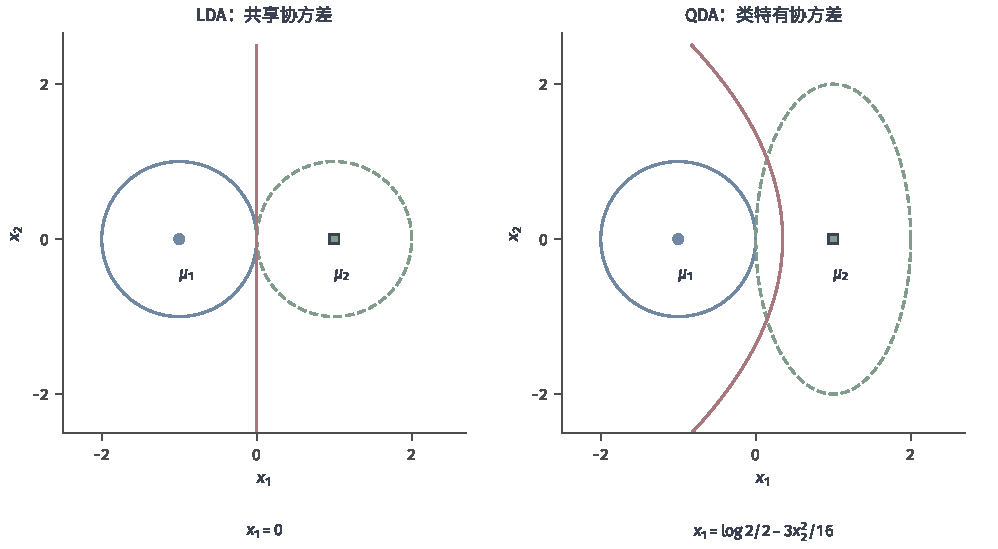
\includegraphics[width=159.059mm]{figures/04-classic-models/00-shared/matplotlib/classification-gaussian-boundaries/figure.pdf}
  \caption{两图均取$\pi_1=\pi_2=1/2$、$\bm{\mu}_1=(-1,0)^{\top}$、$\bm{\mu}_2=(1,0)^{\top}$和$\bm{\Sigma}_1=\bm{I}_2$，仅第2类协方差变化。蓝色圆点和绿色方点为均值，蓝色实线与绿色虚线分别为$\Delta_1=1$和$\Delta_2=1$的等密度轮廓；不同类的这些轮廓不保证密度值相同。红色粗线按$g_1=g_2$的解析式绘制，底部公式分别给出LDA的线性边界与QDA的二次边界。参数均为教学构造，不是采样或拟合结果。}
  \label{fig:classification-gaussian-boundaries}
\end{figure*}

对二分类，把式~\eqref{eq:classification-lda-score}~中的两类得分相减并归一化，就得到Logistic形式的后验。因此，共享高斯假设蕴含线性对数几率，反过来却不成立；许多非高斯输入分布也能有Logistic形式的条件概率。即便两条路线的后验形式相同，用联合似然估计均值和协方差，与直接最大化条件似然，也通常得到不同的有限样本参数。

完整协方差每类需要$d(d+1)/2$个自由参数。类内散布矩阵的秩至多为$n_c-1$，因而$n_c\leq d$时必然奇异，不能直接代入普通高斯密度；$n_c>d$也不保证估计准确或条件良好。共享估计的秩至多为$n-C$。在维数较大或类别样本少时，可以共享、取对角，或采用第\ref{sec:classification-lda-covariance-extensions}节的RDA收缩估计。式\eqref{eq:classification-rda}已经说明这些约束如何借用合并统计量和球形方差；使用收缩就改变了估计准则，不再是未经约束的MLE。

稠密完整协方差的统计成本约为$O(nd^2)$，各类矩阵分解约为$O(Cd^3)$，存储为$O(Cd^2)$，QDA单样本得分约为$O(Cd^2)$。LDA只需分解一份协方差，并可预先算出线性权重，使单样本预测降到$O(Cd)$。实现时可用Cholesky分解求解二次型与对数行列式，无须显式构造逆矩阵。

\subsection{模型对比与总结}
\label{sec:classification-probability-comparison}

Logistic与Softmax直接拟合类别条件概率，NB与GDA先拟合类先验和类条件输入分布。前者不必解释输入怎样产生，后者则可利用分布约束减少需要估计的关系。二分类Logistic是Softmax的两类形式；两者都以互斥类别为对象，多标签任务需要另行规定每个标签事件的模型。

高斯模型的关系由协方差约束决定：QDA允许各类独立的完整协方差，LDA要求共享，高斯NB要求各类协方差对角。LDA与高斯NB各自限制了不同对象，不能一般地按强弱排序。共享高斯模型的共同二次项在类别比较中相消，后验可写成线性Softmax；QDA则需要平方项和交叉项。为Softmax提供这些扩展特征可以表达QDA后验，却无需把系数解释为高斯密度参数。相同的后验形式也不意味着相同学习：联合似然估计与条件似然估计在有限样本上通常选出不同系数。

NB与线性Logistic的联系还取决于事件模型。参数严格为正时，伯努利NB的对数得分累加二值字段，多项式NB的得分按本节文档长度约定累加词项计数，其后验可以写成这些特征上的Softmax。高斯NB在各类单维方差不同时还含有平方项，只是没有跨坐标的交叉项。补集NB改变统计来源，AODE增加部分条件依赖；收缩协方差改变估计约束。这些变化应分别与具体数据缺口比较，不能一律解释成“概率模型更复杂”。

表\ref{tab:classification-probability-comparison}汇总相同监督分类任务下的主要取舍。参数量按每维分布参数有界计算，GDA的共享与类特有协方差分别列明，避免把两者的代价混在一起。
\begin{table}[htbp]
  \centering
  \small
  \begin{tabularx}{\linewidth}{@{}
    >{\RaggedRight\arraybackslash}p{0.19\linewidth}
    >{\RaggedRight\arraybackslash}X
    >{\RaggedRight\arraybackslash}X@{}}
    \toprule
    模型 & 建模与估计 & 主要取舍 \\
    \midrule
    Logistic回归／Softmax回归 &
    直接拟合条件概率；$O(Cd)$个参数，迭代优化 &
    不拟合输入分布；需检查特征表示、分离与正则化 \\
    NB &
    由先验和简化类条件模型形成后验；通常$O(Cd)$个参数 &
    计数或矩估计易累积；依赖和事件模型失配会引入偏差 \\
    共享GDA（LDA） &
    高斯类条件分布，共享协方差；$O(d^2+Cd)$个参数 &
    用共同协方差降低估计波动；只得到线性边界 \\
    类特有GDA（QDA） &
    各类独立估计协方差；$O(Cd^2)$个参数 &
    边界更灵活；对每类样本量和协方差条件更敏感 \\
    \bottomrule
  \end{tabularx}
  \caption{概率分类模型的建模对象与估计代价。所有概率输出都需单独检查校准，参数量不直接等于达到指定精度所需的样本量。}
  \label{tab:classification-probability-comparison}
\end{table}

类条件假设可以减轻小样本下的估计负担，也可能留下模型失配。Ng和Jordan对特定NB与判别式模型的研究展示了这种取舍，不能据此给全部生成式与判别式模型排序\scite{ng2001}。实际选择应固定输入表示、数据划分、误判代价和调参预算，比较分类错误、概率质量与计算成本；训练误差更小或输出取值合法，都不能单独说明概率已经可靠。

\section{半监督分类}
\label{sec:classification-semisupervised}

前面介绍的分类器依靠带标签的样本选择决策边界，但能够收集到的输入往往多于能够完成标注的样本。例如，积累一批待分类文档相对容易，逐篇判断主题却需要人工阅读。如果只使用已经标注的少量文档，其余文档所反映的词语共现和主题聚集结构就没有参与学习。\term{半监督分类}（semi-supervised classification）试图利用这部分信息：由真实标签确定类别含义，再借助未标注输入约束预测规则。

本节把全部$n$个样本的索引分成不相交的有标签集合$L$与无标签集合$U$，满足$L\cup U=\{1,\dots,n\}$。每个输入为$\bm{x}_i\in\mathbb{R}^{d}$，只有$i\in L$时可以在训练中使用真实标签$y_i$；除二分类的专门约定外，类别取值为$\{1,\dots,C\}$。这里的“无标签”描述算法可用的信息，不表示样本在真实任务中没有类别。标签稀缺是学习条件，树、概率模型和间隔模型则描述怎样表示或学习分类规则，因而半监督方法可以与前面几节的模型组合使用。

输入结构与类别之间的联系决定未标注数据能提供什么帮助。同样的两团文档，可能对应两个主题，也可能只因写作风格不同而聚集。分布不匹配、标签采样偏差或未知类别混入，都可能使采用的结构假设失效。Cozman与Cohen对生成式分类器的分析表明，生成模型失配时，加入未标注数据可能增大渐近偏差和分类错误\scite{cozman2002unlabeled}。其结论限定于所分析的生成式模型，指出了核对结构假设的必要性。

Self-Training将筛选后的模型预测作为补充监督，Label Propagation沿相似关系平滑标签得分，TSVM利用输入密度选择间隔边界。三种机制可以共享条件，也可以组合。下面分别说明未标注输入怎样进入训练、目标怎样求解，以及哪些分布联系支撑样本外收益。

\subsection{Self-Training}
\label{sec:classification-self-training}

已经用少量标注文档训练出一个分类器以后，可以先让它预测其余文档。例如，模型对某些包含已知主题词的文档有较高置信度，而这些文档还包含原标注集中少见的其他词。若采纳的类别判断可靠，重新训练就能把这些新词与已有类别联系起来，扩展原来的标签覆盖。

\term{自训练}（self-training）将这个思路组织成外层循环：基分类器产生预测，外层策略筛选部分预测作为补充标签，再扩充训练集并重新拟合。它复用已有分类器，新增的是筛选与重训机制。高置信度也可能来自模型的错误偏好，后面需要检查采纳规则及错误反馈。用机器自身的输出代替部分教师信号的思想，在Scudder于1965年研究的自适应模式识别方法中已经出现；现代筛选、加权和重训方式则可以有许多实现\scite{scudder1965selftraining}。

\subsubsection{模型结构}
\label{sec:classification-self-training-structure}

自训练不要求一种新的决策边界形式。基分类器仍可采用Logistic回归、SVM、决策树或随机森林；新增的部分是怎样管理暂时没有真实标签的样本。为了不混淆真实监督与模型生成的监督，保持原始$L$和$U$不变，用$A^{(t)}\subseteq U$记录第$t$轮已经采纳伪标签的样本索引，用$R^{(t)}=U\setminus A^{(t)}$记录剩余候选池。初始时$A^{(0)}=\varnothing$，模型只在$L$上训练。

假设基分类器以参数$\bm{\theta}$给出类别概率估计$p_{\bm{\theta}}(c\mid\bm{x})$。本节讨论一种阈值筛选方式，把最大类别概率作为\term{置信度}（confidence），即模型对自己当前分类结果的确定程度。对$j\in R^{(t)}$，计算
\begin{equation}
  \label{eq:classification-self-training-selection}
  \begin{aligned}
    \widehat y_j^{(t)}
      &=\argmax_{1\leq c\leq C}
        p_{\bm{\theta}^{(t)}}(c\mid\bm{x}_j),\\
    q_j^{(t)}
      &=\max_{1\leq c\leq C}
        p_{\bm{\theta}^{(t)}}(c\mid\bm{x}_j),\\
    B^{(t)}
      &=\{j\in R^{(t)}:q_j^{(t)}\geq\tau\}.
  \end{aligned}
\end{equation}
其中$\tau$是预先选择的阈值，通常取$1/C<\tau<1$；遇到并列最大值时，本节统一取编号最小的类别。被采纳的预测$\widetilde y_j=\widehat y_j^{(t)}$称为\term{伪标签}（pseudo-label）：它是模型提出的临时训练目标，并没有经过真实标注确认。本节的基本版本在采纳后固定该标签；允许重估或撤销伪标签的版本需要另外规定更新规则。

概率阈值要求筛选分数具有概率含义。SVM得分需先用独立标注数据建立并检验概率映射；直接输出概率的模型也需检查高置信度样本的实际错误率。例如二分类预测$(0.96,0.04)$满足$\tau=0.9$，$(0.55,0.45)$则被保留在候选池。采纳的是模型判为可靠的预测，真实标签仍待另行确认。

\subsubsection{参数学习}
\label{sec:classification-self-training-learning}

每轮采纳伪标签后，基分类器需要重新拟合。以可加权的损失$\ell$为例，当前训练目标可以写成
\begin{equation}
  \label{eq:classification-self-training-objective}
  \begin{aligned}
    \mathcal{J}_t(\bm{\theta})
      ={}&\frac{1}{|L|}\sum_{i\in L}
        \ell\bigl(f_{\bm{\theta}}(\bm{x}_i),y_i\bigr)\\
      &+\frac{\eta}{\max\{1,|A^{(t)}|\}}
        \sum_{j\in A^{(t)}}
        \ell\bigl(f_{\bm{\theta}}(\bm{x}_j),\widetilde y_j\bigr)\\
      &+\beta\Omega(\bm{\theta}).
  \end{aligned}
\end{equation}
这里$L$非空，$\eta\geq0$控制伪标签项的相对权重，$\beta\Omega$沿用基分类器的正则化方式。空伪标签集的求和取零。分别归一化两类样本，是为了避免仅因伪标签数量增加就让它们压过真实标签；若采用统一样本权重，其相对影响会随集合大小改变。对于树等不直接求解这个目标的分类器，可以使用对应的带权拟合接口，自训练的集合更新逻辑不变。

算法\ref{alg:classification-self-training}给出固定阈值、固定已采纳伪标签的版本。$\operatorname{Fit}(A)$表示用真实标签集与索引为$A$的伪标签集完成一次基分类器训练，并返回参数；式~\eqref{eq:classification-self-training-objective}~是这种训练的一种具体实现。算法中省略集合的迭代上标，始终让当前参数对应当前已采纳的训练集。

\begin{algorithm}[带最终重训的自训练]
  \label{alg:classification-self-training}
  \begin{algorithmic}[1]
    \Require 有标签索引$L$、无标签索引$U$及其输入
    \Require 阈值$\tau$、最大扩充轮数$T\geq0$
    \Ensure 分类器$f_{\bm{\theta}}$、已采纳索引$A$和剩余索引$R$
    \State $A\gets\varnothing$，$R\gets U$
    \State $\bm{\theta}\gets\operatorname{Fit}(A)$
    \For{$t=1,\dots,T$}
      \If{$R=\varnothing$}
        \State \textbf{break}
      \EndIf
      \State 用当前模型计算$R$中的$\widehat y_j$与$q_j$
      \State $B\gets\{j\in R:q_j\geq\tau\}$
      \If{$B=\varnothing$}
        \State \textbf{break}
      \EndIf
      \State 保存$\widetilde y_j\gets\widehat y_j$，$j\in B$
      \State $A\gets A\cup B$，$R\gets R\setminus B$
      \State $\bm{\theta}\gets\operatorname{Fit}(A)$
    \EndFor
    \State \Return $f_{\bm{\theta}},A,R$
  \end{algorithmic}
\end{algorithm}

把重训放在集合扩充之后有一个直接作用：无论这一轮恰好用完最大轮数，还是把剩余池清空，返回的模型都已经使用了本轮加入的伪标签。若把训练放在循环开头、随后只添加样本就退出，最后一批伪标签实际上不会影响返回模型。预测前检查空池也很必要，空输入未必被基分类器的批量预测接口接受。当$U$为空或$T=0$时，算法自然返回纯监督模型。

图\ref{fig:classification-self-training}中的反馈箭头将重训后的模型送回预测步骤。真实标签固定在$L$中，未采纳的样本保留在$R$，已采纳的预测保存在$A$；这些集合变化记录监督的来源，使每轮能够区分真实标签与模型生成的伪标签。

\begin{figure*}[htbp]
  \centering
  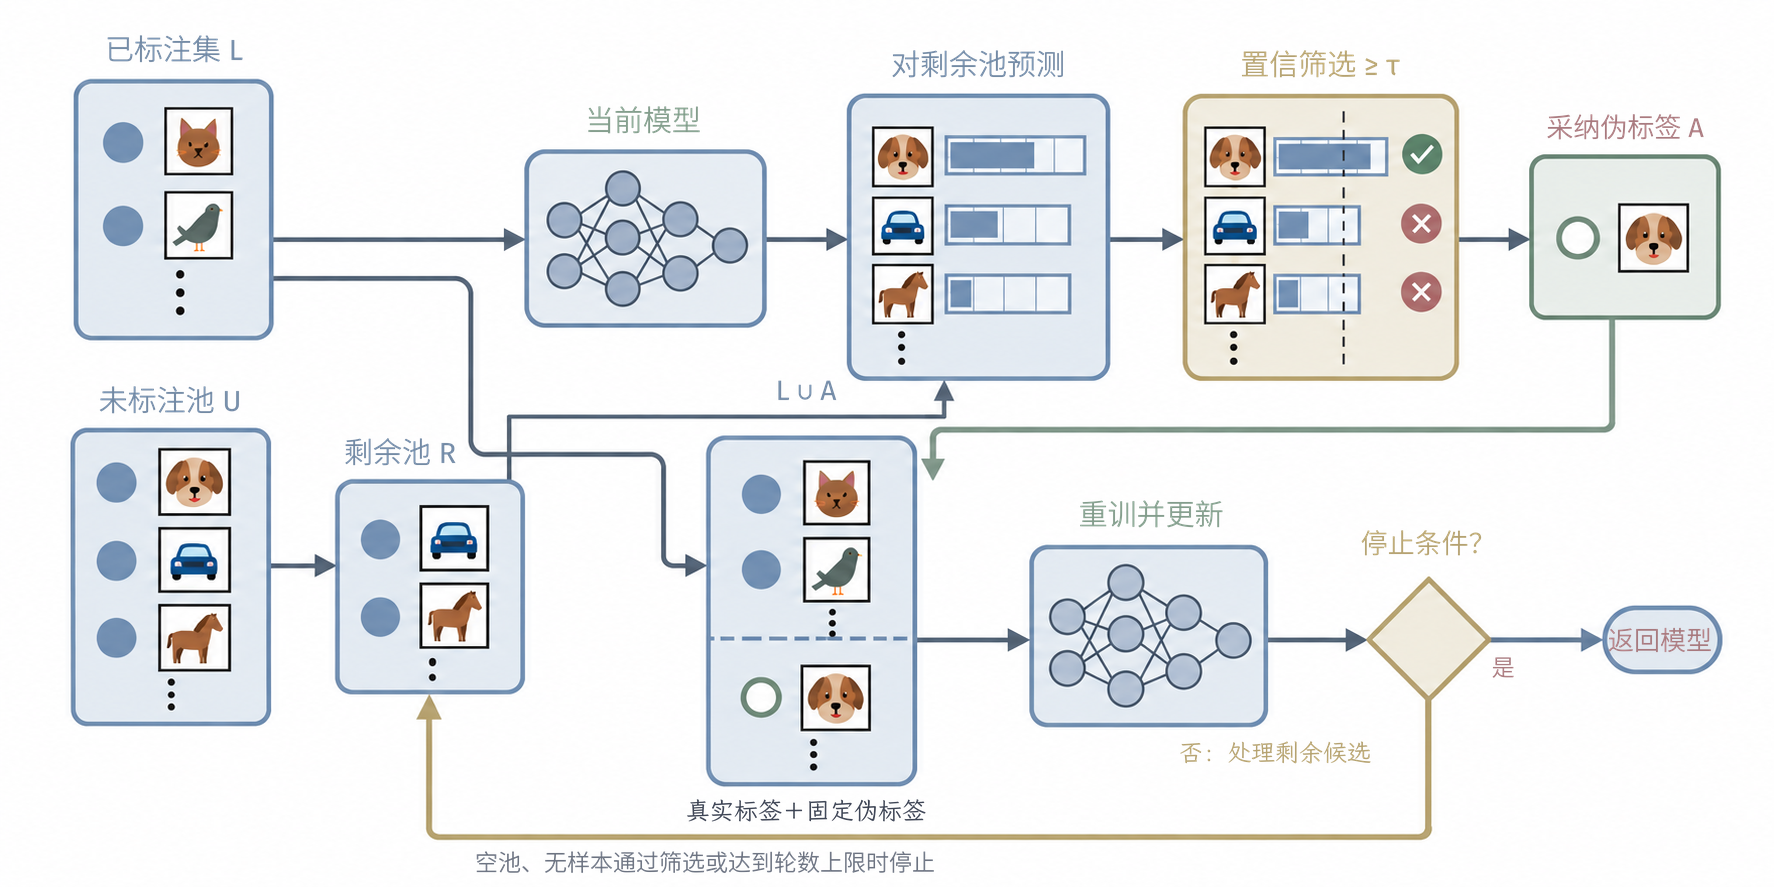
\includegraphics[width=150.199mm]{figures/04-classic-models/00-shared/generated/classification-self-training/figure.png}
  \caption{固定阈值、固定已采纳伪标签的自训练流程，对应算法~\ref{alg:classification-self-training}。真实标签保持不变，已采纳的伪标签始终是模型预测。每次采纳后先重训，再用更新后的模型处理剩余候选；空池、无样本通过筛选或达到轮数上限时停止。这个模型反馈回路也可能产生确认偏差：错误预测被当作后续监督，使模型进一步强化原有误判。}
  \label{fig:classification-self-training}
\end{figure*}

每轮也可以在通过阈值的样本中只取前若干项，限制一次扩充的影响；按类别限制数量则可避免易预测类别占据全部新增监督。这些策略改变$B^{(t)}$的构造，集合更新仍按保存标签、扩充集合、重训的顺序执行。类别配额依据任务中的类别比例设置。

\subsubsection{理论分析}
\label{sec:classification-self-training-analysis}

\paragraph{表达能力}
自训练沿用基分类器的特征与函数形式，候选类不会因增加伪标签而扩大。若基分类器只使用原坐标的仿射得分，前面的四点异或仍不能精确表示，等概率四点上的标签不一致比例至少为$1/4$。加入$x_1x_2$后，得分$-x_1x_2$才使这项目标进入候选类。

\paragraph{收敛性}
这个基本版本何时停止，可以直接从集合变化判断。每次成功扩充至少从$R$移走一个样本，且样本不会移回，因此成功扩充最多发生$\min\{T,|U|\}$次；若没有样本通过筛选，循环会更早结束。只要每次基分类器训练能够返回，外层循环就会有限终止。这一保证针对集合扩充过程的有限终止；各轮训练集和监督信号发生变化，参数优化与统计风险需针对相应模型另行分析。

自训练与\term{熵最小化}（entropy minimization）有共同的倾向：都可能让未标注样本上的预测变得更确定。熵最小化直接惩罚模型预测分布的条件熵，推动概率集中到少数类别。Grandvalet与Bengio讨论了这一准则及其与自训练的联系，这种联系依赖具体的概率模型、筛选和优化设置\scite{grandvalet2004entropy}。

对一个未标注输入$\bm{x}$，Shannon熵与硬伪标签交叉熵分别涉及
\begin{equation}
  \label{eq:classification-pseudolabel-entropy}
  \begin{aligned}
    H_{\bm{\theta}}(\bm{x})
      &=-\sum_{c=1}^{C}p_{\bm{\theta}}(c\mid\bm{x})
        \log p_{\bm{\theta}}(c\mid\bm{x}),\\
    \min_{\widetilde y\in\{1,\dots,C\}}
      \{-\log p_{\bm{\theta}}(\widetilde y\mid\bm{x})\}
      &=-\log\max_c p_{\bm{\theta}}(c\mid\bm{x}).
  \end{aligned}
\end{equation}
前者对所有类别求加权和，后者只取概率最大的一个类别，两者数值和梯度一般不同。例如，预测为$(0.8,0.2)$时，以自然对数计算的熵约为$0.500$，最小硬标签交叉熵约为$0.223$。实际自训练还会筛选样本并冻结历史伪标签，因此下一轮甚至不一定仍以当前最大概率类别为目标。

\paragraph{泛化性}
在同一聚集区域内限制预测差异时，熵最小化倾向于同时提高这些输入的确定性，使边界远离该区域；具体效果依赖基分类器的容量与约束方式。确定性本身仍只描述概率集中程度：若初始模型把同主题文档误判为另一类，采纳后重训可能加强原误判。这种自身错误被重复用作监督的现象称为\term{确认偏差}（confirmation bias）。Arazo等在深度图像分类实验中观察到错误伪标签被拟合，并比较了缓解这一反馈的正则化方法\scite{arazo2020confirmation}。

伪标签错误怎样影响真实风险，可以在固定一轮模型后直接推导。令$h$为这一轮产生伪标签的分类器，$\bm{X}_\tau\subseteq\mathbb{R}^{d}$为通过其置信度阈值的输入区域；$R_{\mathcal P}$沿用目标分布上的零一风险记号。设$\pi=\mathbb{P}_{\mathcal{P}}(\bm{x}\in\bm{X}_\tau)>0$，在筛选区域内分别考察伪标签自身的错误率，以及$f$与伪标签不一致的概率：
\begin{equation}
  \label{eq:classification-self-training-conditional-risks}
  \begin{aligned}
    e_\tau
      &=\mathbb{P}_{\mathcal{P}}
        \bigl(h(\bm{x})\ne y\mid\bm{x}\in\bm{X}_\tau\bigr),\\
    \widetilde R_\tau(f)
      &=\mathbb{P}_{\mathcal{P}}
        \bigl(f(\bm{x})\ne h(\bm{x})\mid\bm{x}\in\bm{X}_\tau\bigr).
  \end{aligned}
\end{equation}
若$f$预测错误，它要么与$h$不一致，要么沿用了$h$的错误，因此
\begin{equation}
  \label{eq:classification-self-training-error-events}
  \{f(\bm{x})\ne y\}
    \subseteq
    \{f(\bm{x})\ne h(\bm{x})\}
    \cup\{h(\bm{x})\ne y\},
\end{equation}
在$\bm{X}_\tau$内应用并集界，再把区域内外的风险相加，得到
\begin{equation}
  \label{eq:classification-self-training-risk}
  \begin{aligned}
    R_{\mathcal{P}}(f)
      \leq{}&\pi\bigl(\widetilde R_\tau(f)+e_\tau\bigr)\\
      &+\mathbb{P}_{\mathcal{P}}
        \bigl(f(\bm{x})\ne y,\ \bm{x}\notin\bm{X}_\tau\bigr).
  \end{aligned}
\end{equation}
式~\eqref{eq:classification-self-training-risk}中的$\widetilde R_\tau(f)$仍是期望不一致损失，不能用训练伪标签上的错误直接替换。若产生标签的模型与新输入池独立，可以把这一步也写成风险界。
\begin{theorem}[自训练在独立输入池与固定候选类下的期望风险界]
  \label{thm:classification-self-training-risk}
  条件于已经训练好的$h$，固定筛选区域$\bm X_\tau$，并在采集本轮伪标签输入前固定含$N\geq1$个分类器的候选类$\mathcal F$。独立抽取$m\geq1$个来自$P_X(\cdot\mid\bm X_\tau)$的输入，以$h$的预测为标签。学习器用这些样本和已有监督返回$\hat f\in\mathcal F$，记其本轮伪标签训练错误为
  \[
    \widehat R_{\mathrm{pseudo}}(\hat f)
      =\frac1m\sum_{j=1}^m
        \mathbb1\{\hat f(\bm x_j)\ne h(\bm x_j)\}.
  \]
  对$0<\delta<1$，关于本轮输入抽样，至少以$1-\delta$的概率，
  \[
    R_{\mathcal P}(\hat f)
      \leq\pi\left[
        \widehat R_{\mathrm{pseudo}}(\hat f)+e_\tau
        +\sqrt{\frac{\log(2N/\delta)}{2m}}\right]
       +(1-\pi).
  \]
\end{theorem}
\begin{proof}
  固定$h$以后，与其伪标签不一致的损失取值于$[0,1]$，其期望是$\widetilde R_\tau(f)$。对本轮独立样本和预定候选类使用有限类的一致偏差界，得到
  $\widetilde R_\tau(\hat f)\leq\widehat R_{\mathrm{pseudo}}(\hat f)
       +\sqrt{\log(2N/\delta)/(2m)}$。
  代入式\eqref{eq:classification-self-training-risk}，再用$1-\pi$上界区域外错误，即得结论。
\end{proof}

这说明即使重训模型完全拟合伪标签，仍要保留采纳区域中的真实错误$e_\tau$和区域外风险。较高的概率阈值本身不提供$e_\tau$的上界；它需要可靠的概率条件或独立真实标签来支持。定理分析的是一轮固定教师、独立输入池和有限候选类；连续参数基模型需要相应容量界。多轮使用同一输入池时，历史伪标签来自不同模型与采纳事件，不能把累积伪标签数直接当作这里的独立样本数$m$。

提高阈值减少采纳量，系统性的高置信度错误仍可能被保留。伪标签权重与单轮规模控制其训练影响，逐类接受率揭示扩充偏向，保留的真实标签验证集则比较扩充前后的效果。验证样本应独立于反复采纳的训练池。未知类别或监督样本覆盖不足时，还需检查数据组成与筛选区域是否符合任务。

\subsubsection{优化泛化能力}

\paragraph{保留未标注类别的不确定性}
\label{sec:classification-self-training-soft-em}

自训练将筛选后的类别作为确定标签；若基分类器已经建立NB或高斯类条件分布，还可以保留类别的不确定性，改用联合似然组织训练。例如，一篇文档当前可能有较高概率属于科技，也有一定概率属于文化，与其立即固定成科技类，不如按两类的后验权重分配它的词频贡献，并在参数更新后重新计算归属。这是生成式半监督方法用潜类别与EM利用未标注输入的路线。它与筛选硬伪标签的自训练使用不同训练目标，不是简单地把筛选阈值调低。

设联合模型为$p_{\bm{\theta}}(\bm{x},y)$，有标签样本直接贡献输入与类别的联合对数似然，未标注样本则只贡献输入的边缘对数似然：
\[
  \ell(\bm{\theta})
  =\sum_{i\in L}\log p_{\bm{\theta}}(\bm{x}_i,y_i)
   +\sum_{j\in U}\log\sum_{c=1}^{C}
      p_{\bm{\theta}}(\bm{x}_j,c).
\]
在这个模型中，全部输入与全部类别合称\term{完全数据}（complete data），其中包括实际未观测的类别；这里的“完全”指连同潜类别一并规定的随机变量。EM在训练时把$U$中的未知类别作为潜变量处理。E步用当前参数计算软后验$q_j(c)=p_{\bm{\theta}^{(t)}}(y=c\mid\bm{x}_j)$；M步最大化当前软后验下的期望完全数据对数似然。记
\[
  \begin{aligned}
    Q(\bm{\theta}\mid\bm{\theta}^{(t)})
    &=
    \sum_{i\in L}\log p_{\bm{\theta}}(\bm{x}_i,y_i) \\
    &\quad+
    \sum_{j\in U}\sum_{c=1}^{C}
      q_j(c)\log p_{\bm{\theta}}(\bm{x}_j,c), \\
    \bm{\theta}^{(t+1)}
    &\in\argmax_{\bm{\theta}}
      Q(\bm{\theta}\mid\bm{\theta}^{(t)}).
  \end{aligned}
\]
只有对多项式NB这类以类别与类别词频为充分统计量的模型，M步才可以解释为把$q_j(c)$作为分数类别计数，与真实标签统计量一起更新先验和类条件参数。此时，未标注文档的词频按$q_j(c)$分配给各类别，而不是先固定成一个不可更改的硬伪标签。Nigam等在文本分类中给出了这一路线的代表性实现\scite{nigam2000text}。

EM改变估计过程，联合分布仍限于预定的$p_{\bm\theta}(\bm x,y)$。选多项式NB就仍使用加性的词频证据，选每类单个高斯就仍不能表达任意多峰类内分布；未标注数据不会替模型补上缺少的依赖项。分布族能够表达真实联合分布时，软类别统计量才有对应的目标参数；这与EM是否找到全局似然最大点仍是两个问题。

模型失配时，大量未标注输入可能加强对错误边缘结构的拟合；Cozman与Cohen对分类性能劣于监督基线的现象给出了分析与实验\scite{cozman2002unlabeled}。后验不能闭式计算时，近似推断又增加了一层误差与计算选择；相应图模型入口见\BookVolumeRef{vol:probabilistic-graphical-models}{卷六“模型：概率图模型”}。

\paragraph{降低伪标签对单个教师的依赖}
同一个模型提出并采纳标签时，系统性偏差可能被重复使用。若输入具有两种各自足以分类的描述，Blum与Mitchell在1998年提出的\term{协同训练}（co-training）可以让两个视图的分类器互供候选标签；其理论设定还要求给定类别后的视图条件独立。没有这种视图关系时，互供标签也可能传播共同错误，且需要训练和评价两个模型\scite{blum1998cotraining}。

没有两种天然视图时，Zhou与Li在2005年提出的\term{三训练}（tri-training）用重采样初始化三个模型，让两个模型的一致预测为第三个提供候选标签，并控制新增标签的错误负担。这增加了模型训练和预测成本，一致意见是否有用仍取决于错误相关性；它改变了监督来源，不是单模型自训练的一项默认设置\scite{zhou2005tritraining}。

\subsubsection{小结}
\label{sec:classification-self-training-summary}

自训练把已有分类器的部分预测转化为新增监督，适合在保留原有训练和预测接口的情况下探索无标签数据的价值。它的额外成本包括对剩余池反复预测，以及在不断扩大的训练集上重新拟合；基分类器训练昂贵时，这些成本并不小。最终模型仍按原分类器的方式预测新样本，无须保留一个独立的传播图。

硬伪标签把当前判断作为后续监督，生成式EM则按当前软类别归属分配统计量，并反复更新联合模型。前者依赖筛选是否可靠，后者还依赖输入分布是否被模型正确描述；两者都可能把错误结构反复写入训练。保留真实标签验证集和针对高代价样本的人工复核，有助于判断新增监督是否值得采纳。

互供标签改变的是新增监督从哪里来。协同训练依靠不同视图，三训练依靠多个模型的一致判断；它们需要更多模型的训练和预测，也要检查共同错误是否被反复采纳。软类别归属与多模型监督来源因此是两个可以分别考虑的方向，不构成由简单到复杂的性能排序。

\subsection{Label Propagation}
\label{sec:classification-label-propagation}

自训练通过基分类器决定哪些预测值得采纳；如果可信的信息主要来自样本之间的邻近关系，也可以直接在这些关系上传递标签。\term{标签传播}（label propagation）把样本表示为图的节点，让已有标签沿相似边影响尚无标签的节点。Zhu与Ghahramani在2002年的技术报告中给出了保持已知标签不变的传播方法\scite{zhu2002labelpropagation}。与只在已标注样本中寻找近邻相比，未标注点也参与形成传播路径，使标签能够沿弯曲的高密度区域传递；每轮恢复已知标签，则让它们持续提供监督，不会因反复平均而失去原有的类别信息。

下面用随机游走解释固定标签边界下的传播，软约束版本随后通过另一目标引入。

\subsubsection{模型结构}
\label{sec:classification-label-propagation-structure}

图模型把“哪些输入相似”转化成可计算的边权。令$\mathcal{G}=(V,E,\bm{W})$，其中$V=L\cup U$，$\bm{W}\in\mathbb{R}^{n\times n}$为非负对称权重矩阵，$\bm{W}_{i,j}=\bm{W}_{j,i}\geq0$，且取$\bm{W}_{i,i}=0$。例如，可以先选出近邻边，再在相连节点上使用RBF相似度
\begin{equation}
  \label{eq:classification-label-propagation-weights}
  \bm{W}_{i,j}=
  \begin{cases}
    \exp\bigl(-\gamma\lVert\bm{x}_i-\bm{x}_j\rVert_2^2\bigr),
      & \{i,j\}\in E,\\
    0, & \text{其他情形},
  \end{cases}
\end{equation}
其中$\gamma>0$控制相似度衰减。用$k$近邻关系构图时，单向近邻关系需要经过并集或互近邻等明确规则转成无向边，才能满足对称性。完全图保留所有样本对，稀疏图只保留选中的关系；两者不仅存储成本不同，也可能给出不同的分类结果。

每个节点的加权度记为$\delta_i=\sum_j\bm{W}_{i,j}$，度矩阵满足$\bm{D}_{i,i}=\delta_i$。在所有参与传播的节点度数为正时，定义
\begin{equation}
  \label{eq:classification-label-propagation-transition}
  \bm{P}=\bm{D}^{-1}\bm{W},
  \qquad
  \bm{P}_{i,j}=\frac{\bm{W}_{i,j}}{\delta_i}.
\end{equation}
矩阵$\bm{P}$每行的和为1，表示从一个节点沿边随机走向邻居的转移概率。传播时用这一行权重对邻居的标签信息求平均；权重大，邻居的影响也大。

为了同时处理$C$个类别，令$\bm{F}\in\mathbb{R}^{n\times C}$保存节点得分，$\bm{f}_i=(\bm{F}_{i,1},\dots,\bm{F}_{i,C})^\top$为节点$i$的得分向量。构造同形状的$\bm{Y}$：若$i\in L$，则$\bm{Y}_{i,c}=\mathbb{1}\{y_i=c\}$；若$i\in U$，则整行置零。有标签节点在每轮更新后都恢复到这份独热编码，这种固定边界的操作称为\term{硬钳制}（hard clamping），也就是不允许传播改变已经给定的标签。

标签边界应能沿图到达每个待预测节点。零度无标签节点没有转移概率，完全无标签的连通分量则缺少类别语义；可补充真实标签、按可靠关系重新构图，或对相应节点拒绝预测。孤立的有标签节点保留原标签。自环或微小度数只能调整数值形式，类别信息仍需要标签边界提供。

\subsubsection{参数学习}
\label{sec:classification-label-propagation-learning}

标签传播没有固定维数的分类器参数要拟合，但需要求出全部无标签节点的得分。下面假设零度节点已经处理，每个含无标签节点的连通分量至少含一个有标签节点。把$\bm{F}$按$L$与$U$分成行块$\bm{F}_L=\bm{F}_{L,:}$、$\bm{F}_U=\bm{F}_{U,:}$，并对$\bm{P}$作对应分块。硬钳制意味着$\bm{F}_L^{(t)}=\bm{Y}_L$始终不变，因而只需迭代
\begin{equation}
  \label{eq:classification-label-propagation-iteration}
  \bm{F}_U^{(t+1)}
    =\bm{P}_{U,U}\bm{F}_U^{(t)}
     +\bm{P}_{U,L}\bm{Y}_L.
\end{equation}
右侧第一项传递尚无标签节点之间的当前信息，第二项持续注入真实标签。通常取$\bm{F}_U^{(0)}=\bm{0}$。真实标签在每轮固定为边界，无标签行按该转移式更新。

若迭代达到固定点，移项便得到线性系统与形式上的闭式解
\begin{equation}
  \label{eq:classification-label-propagation-solution}
  \begin{aligned}
    (\bm{I}-\bm{P}_{U,U})\bm{F}_U^\ast
      &=\bm{P}_{U,L}\bm{Y}_L,\\
    \bm{F}_U^\ast
      &=(\bm{I}-\bm{P}_{U,U})^{-1}
        \bm{P}_{U,L}\bm{Y}_L.
  \end{aligned}
\end{equation}
这里$\bm{I}$为$|U|\times|U|$单位矩阵。本节理论分析将证明，在上述图条件下逆矩阵存在，且任意初始化的迭代都收敛到同一个解。计算时通常直接求解线性系统，避免显式构造逆矩阵。Zhu、Ghahramani与Lafferty给出了这一解的调和函数、图能量和随机游走解释\scite{zhu2003}。

图\ref{fig:classification-label-propagation}给出一个可逐项核算的教学构造，并非实测数据。五个节点依次相连，每条无向边的权重为1；端点1固定属于类1，端点5固定属于类2，节点2、3、4没有标签。令$p_i=\bm{F}_{i,1}^\ast$，由于每个内点恰有两个等权邻居，式~\eqref{eq:classification-label-propagation-iteration}~在固定点处变为
\begin{equation}
  \label{eq:classification-label-propagation-path}
  \begin{aligned}
    p_i&=\frac{p_{i-1}+p_{i+1}}{2},
      &&i=2,3,4,\\
    p_1&=1,\qquad p_5=0.
  \end{aligned}
\end{equation}
内点方程等价于$p_{i+1}-p_i=p_i-p_{i-1}$，所以相邻节点的得分差必须相等。两端总共下降1，分到四条边上，每步下降$1/4$，得到
\[
  (p_1,p_2,p_3,p_4,p_5)
    =(1,0.75,0.5,0.25,0).
\]
类2的得分满足相反的端点条件，故$\bm{f}_i^\ast=(p_i,1-p_i)^\top$。节点2偏向类1，节点4偏向类2；节点3的两类得分相同，按本节“并列时取最小类别编号”的约定判为类1。节点3的类别由并列规则确定，其两类得分所包含的证据仍相同。

\begin{figure}[htbp]
  \centering
  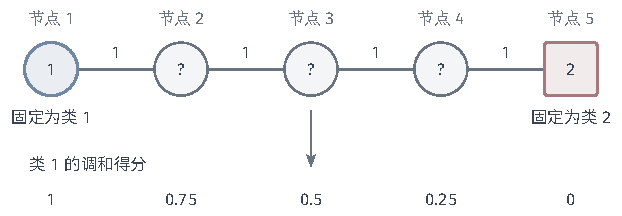
\includegraphics[width=105.315mm]{figures/04-classic-models/00-shared/tikz/classification-label-propagation/figure.pdf}
  \caption{五节点等权无向路径上的硬钳制标签传播。每条边权为1，左端圆形节点固定为类1，右端方形节点固定为类2，问号表示未知标签。下方列出精确调和解的类1得分，类2得分为其补数；内点得分等于两侧邻居的平均。中间节点两类并列，按最小类别编号规则判为类1。这是教学构造，不是实测结果。}
  \label{fig:classification-label-propagation}
\end{figure}

迭代实现还需要把停止条件与返回值对应起来。算法\ref{alg:classification-label-propagation}使用相邻两轮之差作为数值停止判据，其中$\lVert\cdot\rVert_{\mathrm{F}}$为Frobenius范数，$\varepsilon>0$为容限，$T\geq1$为最大迭代次数。达到上限时若尚未满足容限，返回状态记录为未收敛，以便解释当前得分的数值精度。

\begin{algorithm}[硬钳制标签传播]
  \label{alg:classification-label-propagation}
  \begin{algorithmic}[1]
    \Require 权重$\bm{W}$、索引$L,U$、标签矩阵$\bm{Y}$
    \Require 容限$\varepsilon>0$、最大迭代次数$T\geq1$
    \Ensure 得分$\bm{F}$、预测$\widehat{\bm{y}}_U$及停止状态
    \If{$U=\varnothing$}
      \State \Return $\bm{Y}$、空预测、已完成
    \EndIf
    \State 检查$\bm{W}$非负、对称，参与传播的节点度数为正
    \State 检查每个含$U$节点的连通分量至少有一个$L$节点
    \If{任何检查失败}
      \State \Return 拒绝结果，要求补标签或修正传播图
    \EndIf
    \State 构造$\bm{P}=\bm{D}^{-1}\bm{W}$
    \State $\bm{F}_L\gets\bm{Y}_L$，$\bm{F}_U\gets\bm{0}$
    \State $\mathrm{converged}\gets\mathrm{false}$
    \For{$t=1,\dots,T$}
      \State $\bm{G}\gets\bm{P}_{U,U}\bm{F}_U+\bm{P}_{U,L}\bm{Y}_L$
      \State $\Delta\gets\lVert\bm{G}-\bm{F}_U\rVert_{\mathrm{F}}$
      \State $\bm{F}_U\gets\bm{G}$
      \If{$\Delta\leq\varepsilon(1+\lVert\bm{F}_U\rVert_{\mathrm{F}})$}
        \State $\mathrm{converged}\gets\mathrm{true}$
        \State \textbf{break}
      \EndIf
    \EndFor
    \State $\widehat y_j\gets\argmax_c\bm{F}_{j,c}$，$j\in U$；并列取最小$c$
    \State \Return $\bm{F},\widehat{\bm{y}}_U,\mathrm{converged}$
  \end{algorithmic}
\end{algorithm}

算法先把$\bm{G}$保存成最新的$\bm{F}_U$，再判断是否退出，因此即使本轮达到容限，也会返回新得分而不是上一轮的值。相邻迭代差小是一种可操作的停止指标，不直接给出距离精确解的统一误差界；当传播很慢时，还需结合线性系统残差与条件数判断数值精度。最终类别由得分比较决定，接近平局的节点尤其需要保留得分与未收敛状态。

\subsubsection{理论分析}
\label{sec:classification-label-propagation-analysis}

\paragraph{表达能力}
固定图与标签边界时，硬钳制传播的候选得分须满足离散调和条件：标签节点保留给定得分，每个无标签节点的得分等于邻居得分的加权平均。若每个连通分量的真实类别都相同，且给定标签均正确，相应的常值独热得分就满足全部条件，目标因此在这个候选集合中，即使这些分量在原坐标中弯曲。

强连接中的交替标签则可能无法表达。例如，四个节点按$0,1,2,3$组成单位边权路径，节点0的标签为类1、节点3为类2。调和条件迫使两个内部节点的类2得分分别为$1/3$与$2/3$。按最大得分取类，它们只能分别归为类1和类2；若目标类别沿路径依次为1、2、1、2，两个内部节点便都与目标不一致。这一差距来自调和约束，目标所需的交替变化不在候选得分中。

\paragraph{收敛性}
硬钳制传播的收敛来自无标签节点能够沿正权路径到达标签边界。$\bm{P}_{U,U}$的行和至多为1，只有无标签邻居的节点其行和恰为1。因此考察多步后仍留在$U$中的总权重，可以同时处理直接与间接相连的节点。

\begin{theorem}[标签传播在各连通分量有标签条件下解的唯一性]
  \label{thm:classification-label-propagation-convergence}
  设图有限、边权非负且对称，所有参与传播的节点度数为正，$U$非空，且每个含无标签节点的连通分量至少含一个有标签节点。则$\rho(\bm{P}_{U,U})<1$，其中$\rho$表示谱半径。式~\eqref{eq:classification-label-propagation-iteration}~从任意初始得分出发，都收敛到式~\eqref{eq:classification-label-propagation-solution}~中的唯一固定点。
\end{theorem}

\begin{proof}
  从每个$j\in U$出发，选择一条到达$L$的正权路径，并在首次到达$L$时停止。有限图中这些路径长度有一个共同上界$m$，沿各路径行走的概率均为正，其最小值记为$\epsilon>0$。于是，无论从哪个无标签节点出发，在$m$步以内命中$L$的概率都至少为$\epsilon$。这说明
  \[
    \lVert\bm{P}_{U,U}^{m}\rVert_\infty\leq1-\epsilon,
    \qquad
    \rho(\bm{P}_{U,U})^m\leq1-\epsilon<1.
  \]
  因而$\bm{P}_{U,U}^t$趋于零，Neumann级数收敛，且
  \[
    (\bm{I}-\bm{P}_{U,U})^{-1}
      =\sum_{t=0}^{\infty}\bm{P}_{U,U}^{t}.
  \]
  迭代展开为
  \[
    \bm{F}_U^{(t)}
      =\bm{P}_{U,U}^{t}\bm{F}_U^{(0)}
       +\sum_{s=0}^{t-1}
         \bm{P}_{U,U}^{s}\bm{P}_{U,L}\bm{Y}_L.
  \]
  第一项消失，第二项趋于所述固定点。逆矩阵存在，也排除了其他固定点。
\end{proof}

还可以从最优化的角度解释同一个解。相邻节点的得分差越大，图上的不平滑程度越高。令$\bm{L}_{\mathrm{g}}=\bm{D}-\bm{W}$为\term{图拉普拉斯矩阵}（graph Laplacian），它把这种局部差异汇总成二次型。固定真实标签边界后，求解的\term{Dirichlet能量}（Dirichlet energy）最小化问题为
\begin{equation}
  \label{eq:classification-label-propagation-energy}
  \begin{aligned}
    \min_{\bm{F}:\,\bm{F}_L=\bm{Y}_L}\quad
    \mathcal{E}(\bm{F})
      &=\frac12\sum_{i,j=1}^{n}
        \bm{W}_{i,j}\lVert\bm{f}_i-\bm{f}_j\rVert_2^2\\
      &=\operatorname{tr}
        (\bm{F}^{\top}\bm{L}_{\mathrm{g}}\bm{F}).
  \end{aligned}
\end{equation}
第\ref{sec:clustering-spectral}节的谱聚类与第\ref{sec:dim-le}节的拉普拉斯特征映射复用图拉普拉斯和谱工具，但输出分别是离散簇分配与连续低维坐标；这里的标签传播则在已知类别语义下求类别得分。三种任务分别对类别得分、簇分配和坐标施加输出约束。

有标签节点固定为边界，优化变量只包含无标签行。对未知行块求导并令其为零，得到
\begin{equation}
  \label{eq:classification-label-propagation-dirichlet}
  \begin{aligned}
    (\bm{L}_{\mathrm{g}})_{U,U}\bm{F}_U
      &=-(\bm{L}_{\mathrm{g}})_{U,L}\bm{Y}_L\\
      &=\bm{W}_{U,L}\bm{Y}_L.
  \end{aligned}
\end{equation}
因为$(\bm{L}_{\mathrm{g}})_{U,U}=\bm{D}_{U,U}-\bm{W}_{U,U}$，左乘$\bm{D}_{U,U}^{-1}$就回到式~\eqref{eq:classification-label-propagation-solution}~的线性系统。

这个驻点也是唯一最小值，而不只是一个形式上的导数解。取任意无标签节点上的非零向量$\bm{z}$，把它扩展成在$L$上为零的全图向量$\widetilde{\bm{z}}$，则
\[
  \bm{z}^{\top}(\bm{L}_{\mathrm{g}})_{U,U}\bm{z}
    =\frac12\sum_{i,j}\bm{W}_{i,j}
      (\widetilde z_i-\widetilde z_j)^2.
\]
右侧若为零，向量在每个正权连通分量上就必须为常数。每个涉及$U$的分量又含一个值为零的标签边界，因此这些常数只能全部为零，与$\bm{z}\ne\bm{0}$矛盾。故未标记主子块正定，能量对$\bm{F}_U$严格凸。这同时解释了为什么完全无标签的分量会破坏唯一性：在这种分量上，任意常值向量都不增加图能量。

得分的概率含义也需要依赖这些条件。从一个无标签节点按$\bm{P}$行走，并在首次碰到有标签节点时停止，$\bm{F}_{j,c}^\ast$等于首次命中的标签属于类$c$的概率。由于最终命中$L$的概率为1，精确解各行非负且行和为1。若从零初始化，有限轮得分只累积了相应步数内的命中概率，行和可能还小于1；一般不能把尚未收敛的得分直接当成归一化概率。即便在极限处，这也是给定图上的命中概率，不自动等于真实任务中校准的类别后验。

\paragraph{泛化性}
图的统计意义取决于相似关系是否符合类别。\term{平滑假设}（smoothness assumption）要求强边连接的节点具有相近标签得分；文档按写作风格聚集、任务却按主题分类时，这一联系可能失效。跨类强边传播错误信息，错误边界标签还会在每轮持续注入。特征标准化、降维或度量学习可改变高维构图的表示，选择后的图仍需用真实标签验证。

这里还要区分两种评价对象。对非空$U$，在训练之外取得真实标签后，可以计算
\begin{equation}
  \label{eq:classification-label-propagation-pool-risk}
  \widehat R_U
    =\frac{1}{|U|}\sum_{j\in U}
      \mathbb{1}\{\argmax_c\bm{F}_{j,c}^\ast\ne y_j\}.
\end{equation}
其中并列得分仍按最小类别编号处理，$y_j$只用于评价。这个误差评价已经参与构图的输入，未来独立样本需使用另行定义的预测规则。要讨论新样本，还必须定义归纳扩展$h_{\mathcal{G}}(\bm{x})$，即规定新输入如何连接到图、怎样由图上得分产生预测，以及是否重新求解；这时才有相应的风险$R_{\mathcal{P}}(h_{\mathcal{G}})=\mathbb{P}_{\mathcal{P}}(h_{\mathcal{G}}(\bm{x})\ne y)$。

前述唯一解定理确定给定图上的得分。要控制$R_{\mathcal{P}}(h_{\mathcal{G}})$，还需规定归纳扩展，并将构图规则、标签覆盖与类别平滑性联系到目标分布；这些统计条件使给定图上的求解结果具有新样本风险解释。

因此，本节的图能量与唯一解结论没有给出从标注节点训练误差到独立新样本风险的保证。若只固定这批图节点，评价对象就是式\eqref{eq:classification-label-propagation-pool-risk}；若已规定归纳扩展并保留独立测试集，则可以使用后面的定理\ref{thm:classification-semisupervised-test-risk}。两者都不能仅由能量下降推导出来。

\subsubsection{优化泛化能力}

图方法的另一项选择是是否始终保留原标签。硬钳制适合把标签视为可信边界，但标签本身有噪声时，可能希望邻域信息也能调整有标签节点。Zhou等人在2003年的局部与全局一致性方法中给出了软约束传播及其正则化解释\scite{zhou2003consistency}。这类\term{标签扩散}（label spreading）方法使节点在邻域平滑与贴近初始标签之间折中。

在所有节点度数为正的非负对称图上，定义
\begin{equation}
  \label{eq:classification-label-spreading-matrices}
  \bm{S}=\bm{D}^{-1/2}\bm{W}\bm{D}^{-1/2},
  \qquad
  \bm{L}_{\mathrm{sym}}=\bm{I}-\bm{S}.
\end{equation}
$\bm{S}$为对称归一化邻接矩阵，$\bm{L}_{\mathrm{sym}}$为半正定的对称归一化拉普拉斯矩阵，用来衡量按度数归一化后的得分变化。

沿用未标记行置零的初始矩阵$\bm{Y}$，软约束目标为
\begin{equation}
  \label{eq:classification-label-spreading-objective}
  \min_{\bm{F}}\quad
    \operatorname{tr}
      (\bm{F}^{\top}\bm{L}_{\mathrm{sym}}\bm{F})
    +\mu\lVert\bm{F}-\bm{Y}\rVert_{\mathrm{F}}^2,
  \qquad \mu>0.
\end{equation}
第一项约束按度数归一化后的得分在图上平滑，第二项覆盖全部节点，而不只覆盖$L$。在未标记节点上，$\bm{Y}$为零，所以这一项也在约束得分大小。对目标求导并令其为零，得到$[(1+\mu)\bm{I}-\bm{S}]\bm{F}=\mu\bm{Y}$。令$\alpha=1/(1+\mu)$，则
\begin{equation}
  \label{eq:classification-label-spreading-fixed-point}
  \begin{aligned}
    \bm{F}^{(t+1)}
      &=\alpha\bm{S}\bm{F}^{(t)}+(1-\alpha)\bm{Y},\\
    \bm{F}^\ast
      &=(1-\alpha)(\bm{I}-\alpha\bm{S})^{-1}\bm{Y}.
  \end{aligned}
\end{equation}
每轮都在邻居得分与初始标签之间折中，所有节点按同一公式更新，有标签行也不再恢复成$\bm{Y}_L$。重新施加硬钳制会改变目标，需要重新求解。

软约束允许标签得分改变，但仍偏好图上的平滑关系。若单位向量$\bm v$满足$\bm L_{\mathrm{sym}}\bm v=\lambda\bm v$，把一个类别的初始得分列记为$\bm y$、解列记为$\bm f^\ast$，驻点方程给出
\[
  \bm v^\top\bm f^\ast
    =\frac{\mu}{\lambda+\mu}\bm v^\top\bm y.
\]
图能量较大的方向对应较大的$\lambda$，其得分分量被缩小得更多。标签噪声若位于这些方向，平滑可以减弱它；真实类别本来沿强连接变化时，同一个操作也会削弱正确差异。调节$\mu$改变这种取舍，没有从图中产生原本不存在的类别证据。

$\alpha$增大时，图平滑相对于标签拟合的作用增强，某些含噪标签可以被邻居信息修正，也可能把本来正确的少数类标签过度平滑。软得分的行和通常不等于1；按行归一化可以服务于展示或分类接口，但不会自动得到校准概率。完全没有标签的分量在这个软目标下会得到零解，数值上的唯一性仍未赋予它类别信息。因此，软约束的灵活性要与标签噪声和图质量一同评价。

\subsubsection{优化计算能力}

构图和得分求解都需要计算。稀疏图可以减少存储与每轮传播的乘法，但总成本还取决于边数、类别数和迭代次数；连接标签区域的边过弱时，信息传递也可能缓慢。

在合适的相似度矩阵上，\term{Nyström近似}（Nyström approximation）选取少量代表列构造低秩近似，可以减少部分矩阵运算。近似后的非负边权、连通关系与标签边界可能改变，应检查求解误差与分类误差是否仍在可接受范围内。

\subsubsection{支持新输入类别预测场景}

如果希望同时使用图结构并直接预测新输入，可以把图能量施加在分类函数上。\term{拉普拉斯支持向量机}（Laplacian SVM）在监督合页损失之外加入图正则项，要求相似样本上的函数值接近。

以下讨论二分类，将有标签样本的类别编码为$y_i\in\{-1,+1\}$。设$g$属于核$K$的再生核Hilbert空间$\mathcal{H}_K$，$b$为偏置，$\bm{s}$收集全部样本的分数$s_i=g(\bm{x}_i)+b$。采用与本章SVM一致的惩罚记号，一种相应目标是
\begin{equation}
  \label{eq:classification-laplacian-svm}
  \begin{aligned}
    \min_{g\in\mathcal{H}_K,b}\quad
      &\frac12\lVert g\rVert_{\mathcal{H}_K}^2
       +\lambda_{\mathrm{s}}\sum_{i\in L}[1-y_i s_i]_+\\
      &+\frac{\lambda_{\mathrm{g}}}{n^2}
        \bm{s}^{\top}\bm{L}_{\mathrm{g}}\bm{s},
  \end{aligned}
\end{equation}
其中$\lambda_{\mathrm{s}}>0$控制监督合页损失的权重，$\lambda_{\mathrm{g}}\geq0$控制图平滑。真实标签只出现在合页损失中，但图项同时使用$L$与$U$的输入关系；这里不为$U$引入需要离散搜索的标签变量。固定核、图及其超参数后，若核为正定核且图拉普拉斯矩阵半正定，这个目标就是凸的，其优化性质与TSVM的离散非凸搜索不同。

Belkin、Niyogi与Sindhwani在2006年的流形正则化框架中系统给出了这一构造\scite{belkin2006manifold}。

相应解可表示为$g(\bm{x})=\sum_{i=1}^{n}a_iK(\bm{x}_i,\bm{x})$，展开中可以包含有标签和无标签样本。对新输入，按$\hat y(\bm{x})=\operatorname{sign}(g(\bm{x})+b)$判类；沿用第\ref{sec:classification-svm-model}节的约定，零得分预测为$+1$。这样无须先把新输入纳入原图求出一个新节点得分，但仍需承担核展开的存储和计算成本。这里的标量得分与合页损失只对应二分类，多分类须另行组织类别竞争；凸性规定给定目标的求解性质，图质量与相对于监督SVM的收益则由统计条件及评价决定。

图正则化改变核类中的选解偏好，不扩大它能表达的得分族。图项使用全部输入关系，合页损失仍只使用真实标签；应在独立数据上检查平滑是否保留类别差异。

\subsubsection{小结}
\label{sec:classification-label-propagation-summary}

标签传播把相似关系变成图上得分的平滑约束，并用已知标签提供边界。标签扩散允许已有标签得分随邻域一起调整，适合重新考虑含噪监督的权重；若需要直接预测新输入，流形正则化则把图上的平滑要求施加到可在新输入上取值的分类函数。三种做法共享对关系图的依赖，却改变了标签的约束方式和预测对象。

图中错误连接可能削弱真实类别差异，缺少标签覆盖的区域也不会仅靠求解得到可靠类别。选择时应共同考虑构图、传播或核展开的成本，并检查软约束和新输入预测是否符合任务。

\subsection{TSVM}
\label{sec:classification-tsvm}

图传播直接平滑节点得分；若希望保留SVM的分类函数，则可以让无标签样本参与选择大间隔边界。\term{直推支持向量机}（transductive support vector machine, TSVM）同时选择分类器与当前未标注样本的标签，使两类样本共同约束间隔。Joachims在1999年的文本分类研究中给出了有代表性的目标与实用求解算法。其相关性反馈任务说明了这一选择的背景：用户只标注少量检索结果是否相关，其余待分类文档却已经构成一个给定的文档库。于是，这些文档不必等到训练结束后才交给分类器，而可以在训练时通过自身的位置参与确定间隔边界\scite{joachims1999transductive}。

这里的\term{直推学习}（transductive learning，也称转导学习）指利用当前已给定的待预测输入，直接推断这批输入的标签；它与面向未来新输入评价预测规则的归纳设定有所区别。TSVM仍会得到一个SVM分类函数，所以从计算上也能处理新样本。两种评价设定的差异在于参与训练的输入及风险针对的预测集合。

\subsubsection{模型结构}
\label{sec:classification-tsvm-structure}

本小节使用二分类标签$\{-1,+1\}$。令$g(\bm{x})=\bm{w}^{\top}\phi(\bm{x})+b$为决策分数，$\phi$为选定的特征映射；线性SVM取$\phi(\bm{x})=\bm{x}$。标准软间隔SVM只要求已标注样本尽量满足$y_i g(\bm{x}_i)\geq1$。TSVM还为每个$j\in U$引入一个待选择的离散标签$y_j^{\mathrm{u}}$，并为相应间隔约束配置松弛变量$\xi_j^{\mathrm{u}}$。其目标可写为
\begin{equation}
  \label{eq:classification-tsvm-objective}
  \begin{aligned}
    \min_{\bm{w},b,\bm{y}^{\mathrm{u}},\bm{\xi}}\quad
    \mathcal{J}
      ={}&\frac12\lVert\bm{w}\rVert_2^2
         +\lambda_{\mathrm{s}}\sum_{i\in L}\xi_i\\
       &+\lambda_{\mathrm{u}}\sum_{j\in U}\xi_j^{\mathrm{u}},
  \end{aligned}
\end{equation}
其中$\bm{y}^{\mathrm{u}}$收集无标签节点的离散标签，$\bm{\xi}$收集两类松弛变量，$\lambda_{\mathrm{s}}>0$与$\lambda_{\mathrm{u}}\geq0$分别控制有标签项和无标签项的惩罚。约束为
\begin{equation}
  \label{eq:classification-tsvm-constraints}
  \begin{aligned}
    y_i g(\bm{x}_i)&\geq1-\xi_i,
      &\xi_i&\geq0,\quad i\in L,\\
    y_j^{\mathrm{u}}g(\bm{x}_j)&\geq1-\xi_j^{\mathrm{u}},
      &\xi_j^{\mathrm{u}}&\geq0,\quad j\in U,\\
    y_j^{\mathrm{u}}&\in\{-1,+1\},
      &&j\in U,\\
    \sum_{j\in U}\frac{1+y_j^{\mathrm{u}}}{2}&=r.
  \end{aligned}
\end{equation}
最后一行固定无标签样本中的正类标签数量$r$。本节讨论$|U|\geq2$且$1\leq r\leq|U|-1$的非退化情形；$\lambda_{\mathrm{u}}=0$或$U$为空时，分类器训练回到纯监督SVM。

类别数量约束来自一个实际困难：无标签样本本身不能说明哪一侧应有多少样本。若只要求间隔大，模型可能把几乎全部未标注样本放到同一类，从而得到不符合任务的划分。\term{类别平衡约束}（class-balance constraint）把对类别组成的外部知识加入优化，它不要求两类数量相等，而是固定或限制可接受的比例。可以根据可信先验选择$r$，也可以规定$r_{\min}\leq\sum_j(1+y_j^{\mathrm{u}})/2\leq r_{\max}$。由少量已标注样本估计比例时，需要考虑抽样偏差；错误的比例约束同样会损害结果。

数量约束固定待优化标签中的正类数。松弛变量仍允许分类器误分样本或使其落在间隔内，因此标签交换可以保持可行标签数，而重训后的正预测数可能变化。

无标签项怎样影响边界，可以暂时去掉数量约束来观察。对给定分数$s$，若允许独立选择二分类标签，最小的无标签合页损失为
\begin{equation}
  \label{eq:classification-tsvm-unlabeled-hinge}
  \min_{y\in\{-1,+1\}}[1-ys]_+=[1-|s|]_+,
\end{equation}
其中$[a]_+=\max\{a,0\}$。这项损失惩罚分数靠近零的无标签样本，却不预先规定它们应落在哪一侧。在合适的表示下，若大量输入集中在少数区域，让边界避开这些区域就能减少此项损失。这是\term{低密度分离假设}（low-density separation assumption）的作用：类别分界应经过输入较少的区域，而不是切开高密度的同类区域。恢复类别数量约束后，各个标签选择相互耦合，不能再逐样本独立最小化。

\subsubsection{参数学习}
\label{sec:classification-tsvm-learning}

固定$\bm{y}^{\mathrm{u}}$以后，式~\eqref{eq:classification-tsvm-objective}~就是具有不同样本惩罚的软间隔SVM，可以沿用相应凸优化求解器。困难在于标签本身还要选择：固定正类数$r$时有$\binom{|U|}{r}$种标签配置，通常无法逐一求解比较。实用算法从监督SVM出发，交替改善标签与分类器，并逐步提高$\lambda_{\mathrm{u}}$，使无标签数据的影响从弱变强。

初始化也要满足数量约束。先在$L$上训练监督SVM，按它对$U$的决策分数排序，把分数最高的$r$个样本暂定为正类，其余为负类；分数并列时按样本索引排序。监督分类器的正负预测数可能不同于$r$，排序初始化则使数量约束从第一轮开始成立。

在固定$\lambda_{\mathrm{u}}>0$的一轮内，可以交换一个当前正类样本$a$与负类样本$b$的标签。这样正类总数不变，只需判断交换是否有利。记$\ell_{\mathrm{h}}(s)=[1-s]_+$，在当前分类器分数不变时，交换带来的无标签损失变化为
\begin{equation}
  \label{eq:classification-tsvm-swap}
  \begin{aligned}
    \Delta_{a,b}
      ={}&\ell_{\mathrm{h}}\bigl(-g(\bm{x}_a)\bigr)
          +\ell_{\mathrm{h}}\bigl(g(\bm{x}_b)\bigr)\\
       &-\ell_{\mathrm{h}}\bigl(g(\bm{x}_a)\bigr)
          -\ell_{\mathrm{h}}\bigl(-g(\bm{x}_b)\bigr).
  \end{aligned}
\end{equation}
若$\Delta_{a,b}<0$，仅交换标签并相应调整松弛变量，就已经降低了目标中的无标签项；随后重新求解固定标签的SVM，目标值只会进一步降低或保持不变。这个判据识别在当前得分下即可降低损失的交换，搜索范围因此限定于这类变化。

算法\ref{alg:classification-tsvm}采用这一下降判据说明求解过程。$\operatorname{FitSVM}(\bm{y}^{\mathrm{u}},\lambda_{\mathrm{u}})$表示在当前固定标签下，用有标签惩罚$\lambda_{\mathrm{s}}$和无标签惩罚$\lambda_{\mathrm{u}}$完整求解SVM。原始实现还可以为未标注正负类使用不同惩罚；这里用统一的$\lambda_{\mathrm{u}}$突出类别平衡、交换与逐步加权的关系。

\begin{algorithm}[固定类别数量的TSVM逐步加权]
  \label{alg:classification-tsvm}
  \begin{algorithmic}[1]
    \Require 含两个类别的训练索引$L$，无标签索引$U$
    \Require $|U|\geq2$，正类数量$1\leq r\leq|U|-1$
    \Require $\lambda_{\mathrm{s}}>0$，目标$\lambda_{\mathrm{u}}^{\mathrm{final}}>0$
    \Require 初值$\lambda_{\mathrm{u}}^{(0)}>0$，倍率$q>1$，容限$\varepsilon\geq0$
    \Ensure 分类器$g$及离散标签$\bm{y}^{\mathrm{u}}$
    \State 在$L$上训练监督SVM，得到$g$
    \State 按$g$的分数将$U$中前$r$个样本标为正，其余标为负
    \State $\lambda_{\mathrm{u}}\gets
      \min\{\lambda_{\mathrm{u}}^{(0)},\lambda_{\mathrm{u}}^{\mathrm{final}}\}$
    \While{尚未在目标惩罚值下完成训练}
      \State $g\gets\operatorname{FitSVM}(\bm{y}^{\mathrm{u}},\lambda_{\mathrm{u}})$
      \While{存在正负标签对$(a,b)$使$\Delta_{a,b}<-\varepsilon$}
        \State 交换$y_a^{\mathrm{u}}$与$y_b^{\mathrm{u}}$
        \State $g\gets\operatorname{FitSVM}(\bm{y}^{\mathrm{u}},\lambda_{\mathrm{u}})$
      \EndWhile
      \If{$\lambda_{\mathrm{u}}=\lambda_{\mathrm{u}}^{\mathrm{final}}$}
        \State \textbf{break}
      \EndIf
      \State $\lambda_{\mathrm{u}}\gets
        \min\{q\lambda_{\mathrm{u}},\lambda_{\mathrm{u}}^{\mathrm{final}}\}$
    \EndWhile
    \State \Return $g,\bm{y}^{\mathrm{u}}$
  \end{algorithmic}
\end{algorithm}

逐步增加无标签惩罚常称为\term{退火}（annealing）：先在真实标签主导的目标上取得初始解，再逐渐增加无标签约束的影响。这里的每个阶段都先训练并完成交换搜索，再判断是否已经达到最终惩罚值。惩罚更新到目标值后，还需在该值下完成训练与交换搜索，才能返回对应模型。若另设总时间或阶段数量上限，应把提前终止作为未完成目标惩罚训练的状态返回。

这一过程使用上一阶段的结果作初始化，可视为一种延续求解策略，但离散标签变化可能使解发生跳变，不保证存在一条光滑的解路径。退火倍率、初始标签和交换搜索方式会改变最终结果，因此可用多个合理初始化与独立验证比较局部搜索结果。

\subsubsection{理论分析}
\label{sec:classification-tsvm-analysis}

\paragraph{表达能力}
TSVM的候选规则仍由所选线性或核得分族决定。原坐标的线性版本保留异或任务的表示限制，包含交互特征的核版本则可以表达该目标。未标注点的标签是额外变量，却没有为得分函数增加新的输入特征或非线性项。

能够表达真实分界也不要求它位于低密度处。例如，$X$在$[-1,1]$上均匀分布，真实标签由$x$的正负决定，线性得分$g(x)=x$就能精确表示目标。边界附近没有低密度间隙，这一目标仍属于仿射得分族。

\paragraph{收敛性}
固定标签子问题的凸性，不会使标签与参数联合优化也变凸。式~\eqref{eq:classification-tsvm-unlabeled-hinge}~已经显示出其中的非凸性：在$s=-1$和$s=1$处损失均为零，在中点$s=0$处却为1，不满足凸函数的中点不等式。实际问题又包含离散标签及其数量限制，因而是连续变量与离散变量耦合的非凸优化问题。求解一个固定标签的SVM与搜索标签配置，是两项不同的工作。

在固定惩罚值下，算法的有限终止可以有一个明确但有限的保证。假设每次固定标签的SVM都求到全局最小值，并且只接受式~\eqref{eq:classification-tsvm-swap}~所给出的严格下降交换。令$V(\bm{y}^{\mathrm{u}})$为当前标签配置对应的最优目标值，则一次接受交换后有
\[
  V(\bm{y}_{\mathrm{new}}^{\mathrm{u}})
    \leq V(\bm{y}_{\mathrm{old}}^{\mathrm{u}})
      +\lambda_{\mathrm{u}}\Delta_{a,b}
    <V(\bm{y}_{\mathrm{old}}^{\mathrm{u}}).
\]
可行标签配置有限，因此不能在严格下降过程中反复回到同一配置，内层搜索最终会停止。倍率$q>1$并在目标值处截断，也保证外层惩罚阶段有限。这一结论依赖精确子问题求解与严格下降；使用数值近似时，需要检查重训后的实际目标变化，不能只根据理想化推导接受任意交换。

停止只说明当前搜索规则没有找到可接受的改进。即使任何交换在固定$g$时都不下降，也仍可能存在交换后充分重训才改善的解，或者需要同时改变多个标签才能到达的更好配置。因此，这个停止条件既不保证全局最优，也不保证对所有单对交换重训都已最优。不同$\lambda_{\mathrm{u}}$阶段之间的目标函数也不同，跨阶段的目标值不构成同一目标下的下降序列。

\paragraph{泛化性}
统计上的风险来自另一组条件。如果两个真实类别在同一高密度区域内严重重叠，正确的分类边界可能就需要穿过该区域。较大的$\lambda_{\mathrm{u}}$却会奖励避开它的边界，导致无标签数据拉低分类性能。错误的类别比例、未标注池中的未知类别，以及只对局部区域可靠的初始监督模型，也可能产生类似损害。优化更充分并不能修复失效的分布假设，有时反而会更彻底地实现一个不适合任务的目标。

TSVM与监督SVM比较时，固定特征、有标签训练集及评价数据。直推实验允许当前待预测输入参与训练，结果评价这批输入；用于未来输入时，则在独立新样本上另行检验归纳预测。两种设定都使用未参与调参的真实标签计算错误。

先考虑有限池上的直推风险。此时可以允许全部输入参与学习，但标注位置的产生机制仍需明确。下面使用均匀无放回抽样的Hoeffding界控制随机标注位置带来的偏差\scite{bardenet2015sampling}。
\begin{theorem}[TSVM在随机标注位置下的未标注样本期望风险界]
  \label{thm:classification-tsvm-transductive-risk}
  固定$n$个输入及其真实二分类标签。候选预测向量集合$\mathcal V\subseteq\{-1,+1\}^n$由输入和预定模型类确定，不能用真实标签或标注位置来缩小，记$N_{\mathcal V}=|\mathcal V|$。从$n$个位置均匀无放回抽取$\ell$个组成$L$，其中$1\leq\ell<n$，其余$u=n-\ell$个组成$U$。TSVM返回预测向量$\hat h\in\mathcal V$，并以固定规则处理零得分。令$R_U(\hat h)$为在$U$上均匀抽取一个查询位置时的错误概率，$\widehat R_L(\hat h)$为有标签位置上的训练错误。对预定的$\delta\in(0,1)$，至少以$1-\delta$的概率，
  \[
    R_U(\hat h)\leq\widehat R_L(\hat h)
       +\frac n u\sqrt{
          \frac{\log(2N_{\mathcal V}/\delta)}{2\ell}}.
  \]
  对返回的得分$\hat g$，经验项还可放宽为
  $\ell^{-1}\sum_{i\in L}\max\{0,1-y_i\hat g(\bm x_i)\}$。
\end{theorem}
\begin{proof}
  对固定候选向量，$n$个位置上的错误是一个固定的零一总体；$L$上的平均错误是均匀无放回样本平均。无放回Hoeffding界仍给出上尾概率$e^{-2\ell t^2}$。对全部$N_{\mathcal V}$个候选并合，得到同时覆盖它们的事件：总体平均错误$R_{\mathrm{all}}(h)\leq\widehat R_L(h)+t$，其中$t=\sqrt{\log(2N_{\mathcal V}/\delta)/(2\ell)}$。又因
  \[
    R_{\mathrm{all}}(h)
       =\frac\ell n\widehat R_L(h)+\frac u nR_U(h),
  \]
  整理得$R_U(h)\leq\widehat R_L(h)+(n/u)t$。一致事件也覆盖训练后返回的$\hat h$；最后用合页损失上界错分指示量即可。
\end{proof}

例如，预定的$d$维线性TSVM在$n\geq d+1$时，候选预测向量数至多$[en/(d+1)]^{d+1}$，依据是\BookEquationRef{eq:learning-sauer-shelah}{第二卷“基础、理论和可信性”的Sauer--Shelah界}。所以同样概率下，实际输出满足
\[
  R_U(\hat h)\leq\widehat R_L(\hat h)
    +\frac n u\sqrt{\frac{
      (d+1)\log[en/(d+1)]+\log(2/\delta)}{2\ell}}.
\]
这个界不要求标签搜索达到全局最优，也没有证明未标注输入一定带来收益；它把随机标注位置上的经验错误传到了同一输入池的其余位置。主动选择或有偏采集标签不满足均匀抽取假设；高容量核类的$N_{\mathcal V}$可能达到$2^n$，界也可能没有实际约束力。它还没有评价未来独立输入。

对未来输入，一种不依赖TSVM优化过程的检查是在训练和调参完成后使用独立真实标签。
\begin{theorem}[半监督分类器的独立测试风险界]
  \label{thm:classification-semisupervised-test-risk}
  固定训练与调参完成后返回的分类器$f$。取$m\geq1$个独立来自目标分布$\mathcal P$的真实标注测试样本，其输入也不参与训练、特征拟合或模型选择。对预定的$\delta\in(0,1)$，条件于全部训练信息，至少以$1-\delta$的概率有
\begin{equation}
  \label{eq:classification-semisupervised-test-risk}
  R_{\mathcal{P}}(f)
    \leq\widehat R_{\mathrm{test}}(f)
       +\sqrt{\frac{\log(2/\delta)}{2m}}.
\end{equation}
\end{theorem}
\begin{proof}
  条件于训练所得的$f$，每个测试错误都是均值为$R_{\mathcal P}(f)$的独立Bernoulli变量。使用\BookEquationRef{eq:hoeffding-fixed-hypothesis}{卷3《基础、理论与可信性》第5章“二分类学习的可学习性”第5.2节“不可知的有限假设空间”}即可。
\end{proof}
该界也适用于自训练分类器，或已定义归纳扩展的图分类器。它控制的是独立测试抽样偏差，没有证明半监督训练比监督基线更好。$m$计数独立测试样本；若依据这些测试结果继续选择模型，需加入选择校正或保留新的独立测试集。

\subsubsection{优化泛化能力}

若更关心采用无标签数据可能造成的损害，Li与Zhou在2011年研究的\term{安全半监督支持向量机}（safe semi-supervised support vector machine, S4VM）探索多组大间隔候选划分，再按相对于监督基线的最坏净收益选择当前池的输出，并保留基线作为回退。保守选择增加了候选搜索成本，也依赖候选集合能否覆盖需要防备的真实划分；这是一种处理划分不确定性的机制，不能只凭“安全”名称判断实际收益\scite{li2011s4vm}。

\subsubsection{小结}
\label{sec:classification-tsvm-summary}

TSVM保留了SVM的决策函数，把变化集中在训练目标与离散标签搜索中。预测新输入时仍计算$g(\bm{x})$并取其符号；分数恰为零时，应使用预先约定的并列规则。它适用于大间隔与低密度分离有合理联系、类别组成可约束的任务，无标签样本的价值由这些结构联系决定。

TSVM的训练成本来自带权SVM求解与标签交换，受核矩阵、基求解器、惩罚阶段和搜索策略影响。数量约束限制可接受的类别组成，逐步加权利用前一阶段结果作初始化，但这些设置需要符合输入池。搜索得到一组标签，仍应与相同标签预算下的监督SVM比较，再判断低密度边界是否提供了实际收益。

S4VM进一步比较多组候选划分，把相对于监督基线的潜在损害纳入当前池的输出选择。它保留回退的思路，却增加了候选搜索成本；候选集合遗漏真实划分时，保守准则也不能替代缺失的信息。

\subsection{模型对比与总结}
\label{sec:classification-semisupervised-comparison}

未标注输入需要通过某种结构关系才能影响类别判断：已有预测可以补充标签，相似关系可以约束得分，低密度区域可以影响边界位置，联合分布可以提供软类别归属。表\ref{tab:classification-semisupervised-comparison}比较这些信息怎样进入训练，以及需要检查哪些条件。

\begin{table}[htbp]
  \centering
  \small
  \begin{tabularx}{\linewidth}{@{}>{\RaggedRight\arraybackslash}p{25mm}>{\RaggedRight\arraybackslash}X>{\RaggedRight\arraybackslash}X@{}}
    \toprule
    方法 & 无标签数据怎样参与 & 关键条件与代价 \\
    \midrule
    Self-Training & 筛选预测作伪标签，反复训练原分类器 & 采纳的预测应可靠；需反复预测与重训，警惕确认偏差。 \\
    Label Propagation & 在固定标签边界下求图上调和得分 & 图应反映类别关系，且无标签分量能到达标签；成本依赖边数与求解精度。 \\
    TSVM & 联合选择离散标签与大间隔分类器 & 低密度分离及类别数量约束应合理；需要非凸标签搜索与多次SVM训练。 \\
    生成式EM & 把未知类别视为潜变量，按类别软后验累计期望统计量 & 联合模型应足够贴合输入与类别；后验计算与参数更新增加训练成本。 \\
    \bottomrule
  \end{tabularx}
  \caption{四种半监督分类机制的比较。表中列的是使用信息的方式与主要限制，不构成准确率或计算复杂度从低到高的排序。生成式EM与自训练的不同目标见第\ref{sec:classification-self-training-soft-em}节。}
  \label{tab:classification-semisupervised-comparison}
\end{table}

已有监督模型可继续预测新输入时，自训练可以复用它的训练与预测过程，只增加筛选和重训；生成式EM则要求建立联合分布，用输入的边缘似然与软类别归属更新参数。两者即使使用同一个NB基模型，也没有在优化同一目标。协同训练和三训练改变伪标签来源，仍要检验新增标签是否可靠；多个模型的一致意见也可能来自共同偏差。

图方法与TSVM利用的输入关系又不同。标签传播在固定图上平滑节点得分，未规定归纳扩展时，输出只针对已有节点；拉普拉斯SVM把平滑约束施加到核函数，因此能够直接计算新输入的得分。TSVM保留SVM函数，却把未标注类别也作为待选变量，使边界避开相应的高密度区域。图平滑偏好相邻输入得分接近，低密度分离偏好边界位于样本较少处，两项联系可能相符，也可能在错误邻接或类别重叠处失效。应先检查哪项联系在任务中可信，再比较构图、函数求解或离散标签搜索的成本。

这些训练机制并未给出固定的优劣顺序。若要评价未来输入，应使用已经定义的新输入预测规则；若只为当前池选择标签，则按当前池的真实标签评价。S4VM中的监督基线回退也属于后一种输出选择，不能仅凭当前池的保守选择推断未来输入一定获益。两种评价都应保留未参与选择的真实标签，并固定监督预算；无标签数据的数量不能替代类别信息与评价证据。


\Needspace{8\baselineskip}
\section{本章小结}
\label{sec:classification-summary}

分类模型的主要区别在于如何组织类别证据，以及为此学习哪些对象。LDA估计类均值和共享协方差，感知机根据错分修正得分，SVM用间隔约束选择边界；它们的线性形式可以相近，训练准则却不同。近邻保存实例并依赖距离，树与规则学习条件区域，Logistic回归直接拟合条件概率，朴素贝叶斯和GDA先估计类内分布再比较后验。核、局部概率叶、度量学习和相关向量机分别改变特征内积、区域内输出、邻域几何或核展开的估计方法；结构变化之后，学习目标与求解过程也需要随之变化。

半监督方法把未标注输入接入训练的方式同样不同：自训练采用模型预测，标签传播采用图上联系，TSVM寻找穿过低密度区域的边界，生成式EM则估计标签与输入的联合分布。这些联系若与真实类别不符，更多未标注记录也会放大错误。比较时应固定真实标签预算，并与相同监督数据上的基线比较。

邮件过滤还说明，类别、得分和概率需要分别评价：固定拦截规则要看逐类错误和代价，调整阈值要看排序，依据概率分配人工复核资源则要检验概率质量。类别不平衡时应明确汇总口径：宏平均先逐类计算指标再平均，微平均先合并相关计数再计算；分母为零的约定也应写清。具体指标可参考\BookChapterRef{chap:introduction}{卷三《基础、理论与可信性》的“引言”章}；概率校准可参考\BookChapterRef{chap:trust-reliability}{卷三《基础、理论与可信性》的“可靠性”章}。

特征处理和模型拟合在训练数据内完成，超参数、阈值与校准程序通过相应的验证流程选择，最后用独立测试数据评价。比较成本时同时考虑调参、训练和预测：近邻需要检索实例，核展开需要保存相应样本与系数，树和规则则需要执行条件测试。第\ref{chap:clustering}章将撤去预设类别，改为从输入中发现群组；邻域、质心和分布仍会使用，但不再以复现给定标签为目标。

\paragraph{扩展阅读}
Bishop的教材第4章将判别函数、生成式模型和条件概率模型放在同一框架下比较，第7章进一步介绍稀疏核方法。两处内容可用于追踪“得分怎样形成、类别怎样选择、概率怎样估计”之间的联系，并比较估计目标与样本外检验各自承担的作用\scite{bishop2006}。

\chapter{聚类}
\label{chap:clustering}

客户记录没有类别标签时，消费金额相近的人未必购买相同品类，购买品类相近的人也未必有相同频率。\term{聚类}（clustering）先选定要保留的相似关系，再据此寻找群组；这项选择决定了“同一簇”的含义。给定$\bm{x}_1,\ldots,\bm{x}_n\in\mathbb{R}^{d}$，硬划分记为$\mathcal{P}=\{C_1,\ldots,C_K\}$，其中$C_k$是样本索引集合，$c_i=k$表示$i\in C_k$。通常要求簇非空、互斥且覆盖全部样本；噪声、重叠和软归属方法则采用各自的输出约定。

1950至1960年代，中心划分与层次聚类逐渐形成，K-means成为代表方法。1990年代的数据挖掘推动了DBSCAN等密度方法及大规模、子空间聚类；谱方法则从图关系理解群组。概率混合思想有更早的统计来源，19世纪末已用于分析异质总体\scite{clust-macqueen1967,ester1996,clust-pearson1894}。

所需输出可以帮助缩小方法范围。大样本的数值分组和量化可采用K-means及小批量更新；弯曲的密集区域和噪声识别可采用DBSCAN或HDBSCAN；嵌套粒度与成分后验则分别由层次方法和混合模型提供。比较时还需核对距离、密度尺度与分布假设是否符合数据\scite{classic-clustering-guide}。

本章按构造群组的机制展开。原型方法比较样本与代表，邻域和图方法利用连接，网格与子空间方法寻找局部相关结构，层次方法保留嵌套分组，概率方法推断成分归属，半监督方法再加入领域信号。各机制承接第\ref{chap:classic-models-overview}章，也可以共同用于一个模型。

\section{基于原型的聚类}
\label{sec:clustering-partition}

把客户分成 $K$ 组时，可以为每组选择一个代表，并用样本到代表的相异度衡量分组质量。原型聚类最小化这些簇内相异度的总和；各代表竞争样本，形成不同的分配区域。这里的直接目标是组内拟合，簇间分离由分配规则间接产生。

K-means 用均值表示簇，计算方便；K-medoids 用真实样本表示簇，能够使用更一般的相异度。两者共享分配与代表选择的思路，但优化变量和求解方法不同。

\subsection{K-means}
\label{sec:clustering-kmeans}

先考虑图像颜色压缩这个具体任务。每个像素由三个颜色分量组成，如果只能保留$K$种颜色，就需要选出$K$个代表，再把每个像素替换成其中一个。若用替换前后的平方距离为失真计分，一个颜色组的均值恰好使该组的总平方失真最小。\term{K均值聚类}（K-means）把这一做法推广到数值向量：同时寻找$K$个均值中心与样本分配，使总平方距离尽量小。它拟合的是给定表示下的位置，而非预先知道的语义类别。

K-means的目标与更新算法来自多项研究。Steinhaus的《论物质体的分割》刊于第4卷第12期，卷册标为1956年，zbMATH按1957年著录\scite{clust-steinhaus1957}。MacQueen在1967年使用K-means这一名称，讨论逐个吸收样本并立即调整均值的增量算法\scite{clust-macqueen1967}。因此，文献中的K-means有时指平方误差目标，有时指具体求解过程；两种用法需结合更新步骤识别。

本节采用Lloyd的批量更新。它源于信号量化：把连续幅值映射为有限代表值，并控制平方失真。相关工作完成于1957年，经典论文于1982年正式发表\scite{clust-lloyd1982}。Lloyd交替执行最近代表分配与均值重估，每轮使用完整样本；MacQueen则在读入一个样本后立即更新。常见批量实现沿用前一种过程。

平方距离与均值更新使两个条件子问题都容易计算，一轮分配和更新约需 $O(nKd)$ 运算。K-means由此可用于用户分群、向量量化和图像颜色压缩，也可承担谱聚类的离散化或混合模型的初始化。具体用途仍需明确平方失真所代表的损失。

\subsubsection{模型结构}

为第 $k$ 个簇配置中心 $\bm{\mu}_k\in\mathbb{R}^d$，其\term{簇内平方误差}（sum of squared errors, SSE）为
\begin{equation}
  J(\mathcal{P},\bm{\mu})
  =\sum_{k=1}^K\sum_{i\in C_k}
    \lVert\bm{x}_i-\bm{\mu}_k\rVert_2^2.
  \label{eq:clustering-sse}
\end{equation}
这里 $\bm{\mu}=(\bm{\mu}_1,\ldots,\bm{\mu}_K)$ 表示中心参数。固定中心后，每个样本应归入距离最近的中心；固定分配后，每个中心应取簇内均值。

平方欧氏距离的等距离面是球面，最近中心的分配区域是由超平面分隔的Voronoi单元。这样的表示适合在中心附近紧凑分布的群组，环形等非凸群组可能被多个中心拆开。簇的尺度差异也会影响中心数的分配；这些限制来自几何准则，无需假定样本严格服从球形高斯。

\subsubsection{参数学习}

同时优化中心和分配较难，但两个条件子问题都可直接求解。记第 $t$ 轮的分配为 $c_i^{(t)}$，Lloyd 更新写为
\begin{align}
  c_i^{(t+1)}
    &\in\argmin_{1\leq k\leq K}
      \lVert\bm{x}_i-\bm{\mu}_k^{(t)}\rVert_2^2,
      \label{eq:clustering-lloyd-assignment}\\
  \bm{\mu}_k^{(t+1)}
    &=\frac{1}{|C_k^{(t+1)}|}
      \sum_{i\in C_k^{(t+1)}}\bm{x}_i.
      \label{eq:clustering-lloyd-centre}
\end{align}
图~\ref{fig:clustering-lloyd-steps}固定六个样本，分别展示分配与中心更新的作用。中图只重算中心，保留左图的簇标记；右图再比较距离，样本$(1,0)$才由方块簇转入圆点簇。把这两个动作分开展示，才能分别核对每个条件子问题怎样降低目标。

\Needspace{65mm}
\begin{figure*}[htbp]
  \centering
  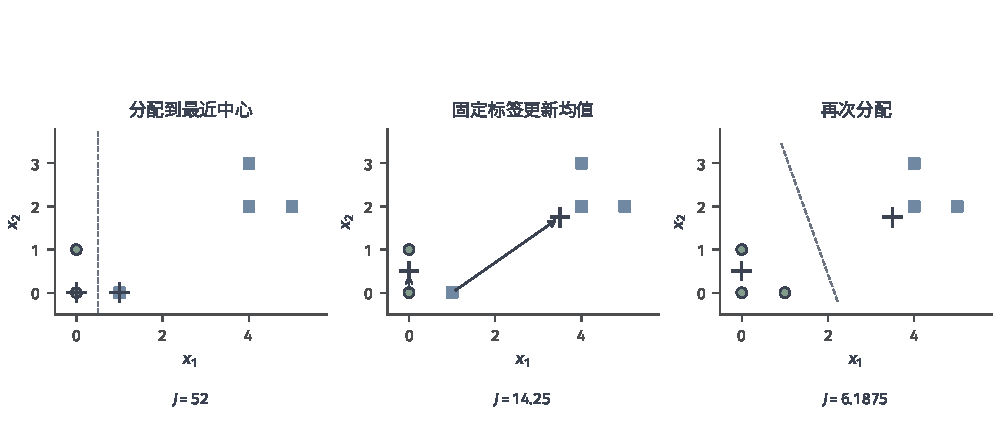
\includegraphics[width=159.059mm]{figures/04-classic-models/00-shared/matplotlib/clustering-lloyd-steps/figure.pdf}
  \caption{Lloyd 迭代的教学例，六个样本为 $(0,0)$、$(0,1)$、$(1,0)$、$(4,2)$、$(4,3)$、$(5,2)$，初始中心为 $(0,0)$ 和 $(1,0)$。圆点与方块表示两个簇，十字表示中心，虚线表示等距边界。首次更新后中心为 $(0,0.5)$ 和 $(3.5,1.75)$；图中依次展示分配、均值更新与再次分配。}
 \label{fig:clustering-lloyd-steps}
\end{figure*}

平局与空簇需要纳入更新规则。等距时优先保留仍属最优的原分配，初始化则按固定顺序决定；空簇没有均值，下面保留其旧中心。这一教学实现最多返回$K$个非空簇。要求恰好$K$个非空簇时，可采用重启或后文的容量约束，并核对相应的停止条件。

\begin{codeblock}[language=Python,label={code:clustering-kmeans}]{带平局与空簇处理的 Lloyd 迭代}
import numpy as np

def kmeans(X, K, max_iter=300, seed=0):
    X = np.asarray(X, dtype=float)
    n = len(X)
    if not 1 <= K <= n or max_iter < 1:
        raise ValueError("invalid K or max_iter")
    rng = np.random.default_rng(seed)
    mu = X[rng.choice(n, K, replace=False)].copy()
    labels = np.full(n, -1)
    for _ in range(max_iter):
        d2 = ((X[:, None] - mu[None]) ** 2).sum(2)
        new = d2.argmin(1)
        rows = np.flatnonzero(labels >= 0)
        keep = d2[rows, labels[rows]] == d2[rows, new[rows]]
        new[rows[keep]] = labels[rows[keep]]
        if np.array_equal(new, labels):
            return labels, mu
        labels = new
        for k in range(K):
            members = X[labels == k]
            if len(members):
                mu[k] = members.mean(0)
    return labels, mu
\end{codeblock}

代码接受有限的二维数值数组。正常停止时，分配与中心形成不动点；迭代上限提前触发时，返回中心已按当前分配更新，但这些分配可能还需再比较一次最近中心。两种退出情形应分别记录。广播计算临时占用$O(nKd)$空间，样本较多时可分块计算距离。

初始中心决定Lloyd从哪里开始搜索。\term{K-means++}先均匀选一个样本，再按$D_i^2/\sum_jD_j^2$抽取后续中心，其中$D_i$是样本到已有中心的最近距离。所有$D_i=0$时，已有中心已覆盖全部不同位置。Arthur与Vassilvitskii证明了初始目标的期望界$\mathbb{E}[J]\leq8(\log K+2)J^\ast$；Lloyd后续不增目标，因此保留这一界\scite{clust-arthur2007}。

该界平均了初始化随机性，单次运行的结果仍可能相差较大。标准K-means++逐个选中心，约需$O(nKd)$运算；分布式实现还需计入数据扫描与通信。评价初始化时，可以同时比较最终平方误差、重启次数和总成本。

\subsubsection{理论分析}

\paragraph{表达能力}
颜色压缩要求用$K$个位置逼近像素分布，因而可以直接用总体平方失真比较候选与目标。只有一个中心时，式\eqref{eq:clustering-mean-decomposition}的总体版本给出
\[
 \inf_{\bm\mu}\mathbb E\lVert\bm X-\bm\mu\rVert_2^2
 =\operatorname{tr}\operatorname{Cov}(\bm X),
\]
条件是输入具有有限二阶矩，最优中心为总体均值。增加中心可以降低这个最小失真；固定$K$时，只有分布集中在至多$K$个位置上，才能把平方失真降为零。例如，将$[0,1]$上的均匀分布用$K$个标量量化，最优中心为等长区间的中点，最小期望失真为$1/(12K^2)$。长度为$\ell$的区间在其中点处贡献$\ell^3/12$，所有区间长度之和为1，凸性使等长划分达到最小值。这个例子明确给出了中心数增加时，模型与量化目标之间还剩多少误差。

客户群组的语义若由另一种关系决定，低失真便未必代表准确分组。比较中心$\bm\mu_a,\bm\mu_b$时，归入前者的条件等价于
\[
 2(\bm\mu_b-\bm\mu_a)^\top\bm x
 \leq\lVert\bm\mu_b\rVert_2^2-\lVert\bm\mu_a\rVert_2^2.
\]
一个簇是这些半空间的交，因而是凸的Voronoi单元。假设目标是把完整的内外同心圆分别分成两簇。包含整个外圆的凸单元必然包含其内部圆盘，不能同时排除内圆；两个中心无论怎样优化，都不能准确表达这个目标。增加中心可以把外圆分成多段，却改变了“一圈一簇”的输出。两片大小或样本比例不同的区域也可能获得不同数量的中心，因为目标按概率质量累加平方失真，并未要求每个语义群体恰用一个中心。Mini-Batch只近似更新相同的中心，不能消除这些表达限制。

\paragraph{收敛性}
Lloyd的有限停止需要目标下降与平局规则共同支持。目标有下界且不增，足以得到目标值的极限；进一步排除无穷次分配变化，才可得到有限轮停止。下面利用有限分配集合完成这一步。

\begin{theorem}[K-means的Lloyd迭代在严格下降条件下的有限停止]
  \label{thm:clustering-lloyd}
  对有限样本，在精确计算下，分配步采用最近中心规则，并在平局时优先保留原簇分配；更新步对非空簇取均值、对空簇保留旧中心。则目标值单调不增，算法在有限轮后到达分配和中心均不再变化的不动点。
\end{theorem}
\begin{proof}
固定中心，逐点选择最小距离给出
\[
 J(\mathcal{P}^{(t+1)},\bm{\mu}^{(t)})
 \leq J(\mathcal{P}^{(t)},\bm{\mu}^{(t)}).
\]
对任意非空簇 $C$，记均值为 $\bar{\bm{x}}_C$。展开平方项，并利用 $\sum_{i\in C}(\bm{x}_i-\bar{\bm{x}}_C)=\bm{0}$，得到
\begin{equation}
 \sum_{i\in C}\lVert\bm{x}_i-\bm{a}\rVert_2^2
 =\sum_{i\in C}\lVert\bm{x}_i-\bar{\bm{x}}_C\rVert_2^2
   +|C|\lVert\bm{a}-\bar{\bm{x}}_C\rVert_2^2.
 \label{eq:clustering-mean-decomposition}
\end{equation}
所以均值是唯一最优中心，更新步也不会增加目标；空簇对目标贡献为零。

第一次均值更新后，若分配改变，至少一个样本移向严格更近的中心，否则保留原标签的规则会阻止改变。因此完整一轮使目标严格下降。对任一分配，均值更新后的目标只由该分配决定，即使存在空簇也如此。分配至多有 $K^n$ 种，严格下降不可能无限次访问它们。分配不变时，已有非空簇中心仍为相同均值，算法遂停止。
\end{proof}

不动点在固定中心时满足最近分配，在固定分配时满足均值最优。若每个样本的最近中心唯一、各簇非空，则足够小的中心扰动保持分配，均值最优性给出局部最优解释。等距样本或重合中心可能破坏这一局部稳定条件，需按退化结构分析。

两个子问题易解，联合的全局搜索仍可能昂贵。维数属于输入时，固定$K=2$的欧氏平方和聚类已是NP-hard\scite{clust-aloise2009}。平面上将$K$作为输入也有NP-hard结果\scite{clust-mahajan2012}。这些结果表明，在$\mathrm{P}\ne\mathrm{NP}$的前提下，一般输入的精确全局解无法统一用多项式时间取得。

\paragraph{泛化性}
学到的中心将怎样处理下一批像素，可以直接用新像素到最近中心的平方距离回答。以下沿用经验风险$\widehat R_n$与期望风险$R$的记号，训练样本$D_n=(\bm X_1,\ldots,\bm X_n)$独立同分布于$P$，风险中的$\bm X\sim P$独立于$D_n$。取$r>0$，将候选中心限制在半径$r$的球内，并假设$\lVert\bm X\rVert_2\leq r$几乎处处成立。此时
\[
 \ell_{\bm\mu}(\bm x)=\min_{1\leq k\leq K}
       \lVert\bm x-\bm\mu_k\rVert_2^2,
 \qquad R(\bm\mu)=\mathbb E_P\ell_{\bm\mu}(\bm X).
\]
这一风险衡量颜色量化失真，尚未涉及簇的语义是否正确。有限样本保证需要同时控制候选中心的数量尺度和求解误差。下面先给出后者如何进入风险界的共同步骤。

\begin{lemma}[有限覆盖下的期望风险界]
 \label{thm:clustering-cover-risk}
取预定的置信参数$\delta\in(0,1)$。
 设$D_n$由$n$个独立同分布观测组成，候选集$\Theta$及其度量在抽样前固定，损失取值于长度为$M$的固定区间，并满足
 $|\ell_\theta(\bm x)-\ell_{\theta'}(\bm x)|\leq L\,d(\theta,\theta')$。
 对任意$\epsilon>0$，设$\Theta$有一个含$N_\epsilon$个点的$\epsilon$覆盖，即每个候选到某个覆盖点的距离至多为$\epsilon$。
 学习器输出$\widehat\theta$，其经验求解误差为
 \[
  e_n=\widehat R_n(\widehat\theta)
          -\inf_{\theta\in\Theta}\widehat R_n(\theta)\geq0.
 \]
 则以至少$1-\delta$的训练抽样概率，
 \begin{equation}
  R(\widehat\theta)-\inf_{\theta\in\Theta}R(\theta)
  \leq4L\epsilon
       +2M\sqrt{\frac{\log(2N_\epsilon/\delta)}{2n}}
       +e_n.
  \label{eq:clustering-cover-risk}
 \end{equation}
 对训练样本及学习器随机性取期望，也有
 \[
  \mathbb E_{D_n}R(\widehat\theta)-\inf_{\theta\in\Theta}R(\theta)
  \leq4L\epsilon
       +2M\sqrt{\frac{\log(2N_\epsilon)}{2n}}
       +\mathbb E_{D_n}e_n.
 \]
\end{lemma}
\begin{proof}
在覆盖点上，Hoeffding界与并集界给出
$\max_\theta|R(\theta)-\widehat R_n(\theta)|
 \leq M\sqrt{\log(2N_\epsilon/\delta)/(2n)}$。
对任意候选，分别将期望风险和经验风险移到最近覆盖点，至多各增加$L\epsilon$，所以全体候选上的偏差至多为
$\Delta_n=2L\epsilon+M\sqrt{\log(2N_\epsilon/\delta)/(2n)}$。
在$R(\widehat\theta)-\inf_\theta R(\theta)$中加入两侧经验风险，得到
$R(\widehat\theta)-\inf_\theta R(\theta)\leq2\Delta_n+e_n$。
期望结论使用同一分解，并对覆盖点的$2N_\epsilon$个带符号偏差应用Hoeffding指数矩界，得到最大偏差的期望至多为
$M\sqrt{\log(2N_\epsilon)/(2n)}$。
\end{proof}

\begin{theorem}[K-means在有界输入下的期望量化风险界]
 \label{thm:clustering-kmeans-risk}
设$D_n$独立同分布于$P$，$\lVert\bm X\rVert_2\leq r$，$r>0$，固定$K$且中心范数至多为$r$。对K-means，损失位于$[0,4r^2]$，用各中心移动距离的最大值衡量两组中心的差异时，$L=4r$。每个$d$维球有至多$(1+2r/\epsilon)^d$个覆盖点，$K$个中心因而有$N_\epsilon\leq(1+2r/\epsilon)^{Kd}$。取$\epsilon=r/n$，式\eqref{eq:clustering-cover-risk}给出
\begin{equation}
 \mathbb E_{D_n}R(\widehat{\bm\mu})
 \leq \inf_{\lVert\bm\mu_k\rVert_2\leq r}R(\bm\mu)
   +\frac{16r^2}{n}
   +8r^2\sqrt{\frac{Kd\log(1+2n)+\log2}{2n}}
   +\mathbb E_{D_n}e_n.
 \label{eq:clustering-kmeans-risk}
\end{equation}
概率至少为$1-\delta$的版本将$\log2$换成$\log(2/\delta)$，并保留实际运行的$e_n$。
\end{theorem}

这里比较的是同一候选中心集中的最佳总体量化误差，无需总体最优中心唯一。中心投影到该球不会增加球内样本的距离，因此这一限制也不损失该设定下的全局最优值。

经验到总体的推理现在有三步：同时控制所有中心的经验偏差，利用学习器在经验目标上的质量，最后比较总体目标。精确经验全局解使$e_n=0$；一次Lloyd或小批量运行只得到局部或近似解，其$e_n$仍须计入，增加样本不能自动消除这一项。Pollard的一致性结果进一步研究最优中心本身的极限\scite{clust-pollard1981}。式\eqref{eq:clustering-kmeans-risk}则直接评价新样本损失。

输入表示同样影响这个损失。平方距离放大远离中心的样本，不同量纲改变最近中心的次序，因此尺度选择需对应业务含义。第\ref{sec:regression-knn}节的$k$-NN回归也依赖距离，但它平均带响应的邻居，K-means拟合无标签输入的位置。

\subsubsection{优化表达能力}

中心分配的形状也受表示限制。考虑围绕同一圆心的内外两圈样本，两圈的均值都靠近圆心，用两个原空间中心难以按半径分开它们。若以半径平方作为一个新特征，内外圈在该坐标上就落在不同位置。\term{核 K-means}（kernel K-means）采用相同思路，在特征映射$\phi$之后比较样本与簇均值。第\ref{sec:classic-overview-kernel-trick}节的正定核$K$允许我们直接计算这些距离；映射是否适合当前群组，仍由核的选择决定。样本到簇均值的平方距离为
\begin{equation}
 \begin{aligned}
 \lVert\phi(\bm{x}_i)-\bm{\mu}_k^\phi\rVert^2
 ={}&K(\bm{x}_i,\bm{x}_i)
 -\frac{2}{|C_k|}\sum_{j\in C_k}K(\bm{x}_i,\bm{x}_j)\\
 &+\frac{1}{|C_k|^2}
   \sum_{j,l\in C_k}K(\bm{x}_j,\bm{x}_l).
 \end{aligned}
 \label{eq:clustering-kernel-kmeans}
\end{equation}
公式只使用核值，省去了显式构造$\phi$，相应成本转为核矩阵计算与存储\scite{clust-girolami2002,dhillon2004}。Girolami讨论核空间聚类，Dhillon、Guan与Kulis进一步联系了适当权重和核构造下的核K-means与归一化割。

同心圆的例子可以核验映射带来的收益。对半径分别为$r_1,r_2$的两个完整圆，取$\phi(\bm x)=\lVert\bm x\rVert_2^2$，对应的正定核为$K(\bm x,\bm y)=\lVert\bm x\rVert_2^2\lVert\bm y\rVert_2^2$。两圈分别变为标量$r_1^2,r_2^2$，用两个中心可得到零特征失真，并准确保留“一圈一簇”。若两组半径存在重叠，仅保留这个特征就无法区分重叠位置；若目标按角度分组，它还会把同半径的不同群组混在一起。核技巧让特定非线性关系进入候选范围，效果需要对应目标，而不能由“采用了核”单独保证。

核K-means与归一化割的联系依赖适当的权重和核构造，适用范围需随具体等价关系核对。特征映射可以改变原空间的分配形状，层次结构则改变输出粒度；多层输出见第\ref{sec:clustering-hierarchy}节，局部密度与连接提供了另一种描述弯曲群组的方式。

\subsubsection{优化泛化能力}

中心的选择还取决于怎样评价距离。用一个固定簇的单坐标教学例子看：数据为$0,0,0,100$时，平方距离和在均值$25$处最小，绝对距离和则在中位数$0$处最小。极端记录可以把均值拉离多数样本，改用绝对距离就改变了这种牵动。\term{K 中位数聚类}（K-medians）最小化$\ell_1$距离和，固定分配后逐坐标取中位数；它不等于以欧氏距离和定义的几何中位数问题。

在这个例子中，单中心的最小绝对距离和为100，而在均值25处为150；反过来，中位数处的平方距离和为10000，均值处为7500。因而改用中位数改善的是绝对距离目标，不能据此宣称对平方量化也更准确。多维$\ell_1$损失逐坐标相加，适合目标确实要求累加各坐标绝对偏差的情形；它没有利用坐标间的相关方向，也没有为弯曲群组增加新的连接表示。

\subsubsection{优化计算能力}

颜色压缩若涉及大量图像，一次中心更新就要重新比较全部像素与$K$个中心，即使中心只移动一点，也要付出一次全量扫描的成本。\term{小批量K均值聚类}（Mini-Batch K-means）改用抽取的$b$个样本估计更新方向，只调整这些样本涉及的中心。Sculley在2010年研究了这一方法\scite{clust-sculley2010}。平方距离目标仍然保留，每轮采用的信息量与计算量则减少了。

设簇 $k$ 累计接收了 $v_k$ 次样本更新。每接收一个分配到该簇的样本，就令 $v_k\leftarrow v_k+1$，并计算
\begin{equation}
 \bm{\mu}_k\leftarrow
 (1-\eta_k)\bm{\mu}_k+\eta_k\bm{x}_i,
 \qquad \eta_k=\frac{1}{v_k}.
 \label{eq:clustering-minibatch}
\end{equation}
这是对历史已分配样本的增量平均，不是当前全体簇成员的精确均值。一轮距离计算降为 $O(bKd)$，但总成本仍取决于迭代次数、初始化和最终全量分配。

随机小批量使每次更新只反映部分样本，逐轮全量SSE可能波动。批量大小、采样偏差和低频簇的覆盖影响最终误差；定理~\ref{thm:clustering-lloyd}针对完整分配与精确均值更新，其单调性前提在这里发生改变。选择计算预算时，应以抽样评价或留出量化误差检查这种近似是否足够。

\subsubsection{支持簇容量约束场景}

\label{sec:clustering-capacity}

用于服务网点分配时，最近中心规则还可能违反容量要求。假设一个网点最多服务100条客户记录，它附近却有150条记录；把这些记录全部分给最近网点可以减小SSE，却使方案无法执行。限制簇大小的方法把每簇的最小与最大容量加入分配条件，再在可行方案中比较距离。Bradley、Bennett与Demiriz研究了带最小簇规模的K-means；加入上界后，固定中心的分配问题可统一写为\scite{clust-bradley2000}。
\begin{equation}
 \begin{aligned}
 \min_{\bm{Z}}\quad&
   \sum_{i=1}^n\sum_{k=1}^K
   z_{i,k}\lVert\bm{x}_i-\bm{\mu}_k\rVert_2^2,\\
 \text{s.t.}\quad&
   \sum_{k=1}^K z_{i,k}=1,\quad z_{i,k}\in\{0,1\},\\
 & \ell_k\leq\sum_{i=1}^n z_{i,k}\leq u_k.
 \end{aligned}
 \label{eq:clustering-capacity}
\end{equation}
整数容量满足 $0\leq\ell_k\leq u_k$，且在没有其他分配禁令时，可行性条件为 $\sum_k\ell_k\leq n\leq\sum_ku_k$。

固定中心的容量分配可转为最小费用流。源点到每个样本的边容量为1，样本到每簇的边容量为1、费用为平方距离，簇到汇点的边下界为$\ell_k$、上界为$u_k$，总流量为$n$。网络流的整数性保证存在整数最优解，使每个样本恰好选择一簇；这一性质来自网络约束的结构。

容量方法的中心仍按均值更新。每次分配精确最优且平局保留已有最优分配时，分配变化导致严格下降；采用确定的空簇处理后，可按有限分配集合证明停止。求解成本取决于网络规模、费用表示与求解器，需按具体实现估计。

Malinen 与 Fränti 在 2014 年研究了要求簇规模相等的平衡 K-means\scite{clust-malinen2014}。当 $K$ 整除 $n$ 且要求 $|C_k|=n/K$ 时，把每个中心复制成相应数量的容量槽，得到 $n$ 对 $n$ 的指派问题；Hungarian 算法可在 $O(n^3)$ 时间内求解。

当$n$不能被$K$整除，可为各簇指定$\lfloor n/K\rfloor$或$\lceil n/K\rceil$个槽，并使容量总和为$n$。按距离顺序填槽可以节省搜索，却可能让先处理的样本占用后续样本所需位置。使用这种启发式时，还需检查全部下界与实际SSE变化。

容量约束表达的是一批对象共同满足的分配要求。若目标方案满足给定上下界，它仍在候选范围内；若一个目标簇有150条记录而上界为100，这个簇就必须拆开或让部分记录转组。受约束的最小SSE不小于无约束的最小SSE，增加的失真是满足容量的代价。此时一个样本的归属取决于其他样本占用了哪些槽，不能再把训练划分解释成独立的最近中心区域。对新的一批客户执行相同容量要求，还需要共同求解分配。

\subsubsection{支持模糊隶属度输出场景}

最近中心规则只给出一个簇标签，无法表达样本处于两个群组之间的程度。例如，一位客户的购买行为同时接近两类典型客户，略微改变记录就可能使硬标签跳到另一类。\term{模糊 C 均值}（Fuzzy C-Means, FCM）保留各中心之间的比较，用隶属度$u_{i,k}$分配软归属，因而可以表达这种过渡\scite{clust-bezdek1981}。
\begin{equation}
 J_{\mathrm{FCM}}
 =\sum_{i=1}^n\sum_{k=1}^K
 u_{i,k}^{q}\lVert\bm{x}_i-\bm{\mu}_k\rVert_2^2,
 \quad \sum_k u_{i,k}=1,\quad q>1.
 \label{eq:clustering-fcm}
\end{equation}
这里$q$控制隶属度的模糊程度。固定隶属度时，中心是以 $u_{i,k}^q$ 为权重的均值；当各距离非零时，固定中心给出
\[
 u_{i,k}=
 \left[
 \sum_{j=1}^K
 \left(\frac{\lVert\bm{x}_i-\bm{\mu}_k\rVert_2}
 {\lVert\bm{x}_i-\bm{\mu}_j\rVert_2}\right)^{2/(q-1)}
 \right]^{-1}.
\]
若样本与一个或多个中心重合，可把隶属度集中在这些零距离中心上。隶属度表示模糊目标下的软归属；赋予生成后验含义还需要相应概率模型。医学影像中一个像素混合多种组织的部分体积效应，可为这种软表达提供应用动机。

FCM能够表达的软关系仍由中心距离约束。两个距离相等且非零时，两者的隶属度相等；所有$K$个距离相等时，各隶属度必为$1/K$。若两类在该位置的真实比例并不相等，仅调$q$不能让这个规则给出所需比例，因为$q$只改变距离比的指数。对内外同心圆，若两个中心都取圆心，两圈上的每个点都会得到相同的均匀隶属度，无法表示半径决定的成分归属。软输出补充了边界过渡，却没有自动补充形状或生成比例。

\subsubsection{支持层次划分输出场景}

若除了最终的$K$组，还希望看到“先分成哪两大组，再怎样细分”，一次性$K$中心划分没有保留这种关系。\term{二分 K-means}（Bisecting K-means）从全部样本组成的一簇开始，反复选择一个簇作$K=2$划分。常见实现选择最大SSE的簇，并为每次二分多次重启。分裂记录形成一棵层次树，但早期分开的对象以后不能跨分支重组，最终SSE因而不保证优于一次性$K$分。Steinbach等在文档聚类中研究了这一方案\scite{clust-steinbach2000}。

每次最近双中心分裂都增加一个半空间条件，最终叶簇是沿路径得到的半空间交，仍为凸区域。它可以表示不同粒度下相互包含的群组；若某个目标群组跨越了早期切面，后续细分只能把它切成更多片，不能重新组成一簇。因此，层次输出增加了可解释的粒度关系，并未消除原空间中心划分对环形目标的限制。

\subsubsection{小结}

K-means适合把数值记录压缩成有限个中心，平方距离规定了怎样比较压缩误差。使用前应先确定各坐标的尺度与$K$的含义：用于颜色量化时，中心代表可用颜色；用于客户分析时，最近中心形成的群组还需要业务证据解释。

围绕同一个平方误差目标，可以分别调整计算与可行分配。小批量更新只访问部分记录，节省每轮扫描，但需要检查低频簇的覆盖与最终失真。容量约束把“网点能接收多少客户”写入分配问题，得到可执行的方案，同时增加共同分配的求解成本，并可能增加距离损失。

其他调整改变了所要表达的群组。绝对距离减弱极端记录对中心位置的牵动，FCM允许边界样本软归属，二分方案保留层次，核表示则改变比较样本的坐标。它们分别改变损失、输出粒度或表示，不能互相替代：软标签未消除单中心的形状限制，核映射也需要保留任务所需的区别。

\subsection{K-medoids}
\label{sec:clustering-kmedoids}

均值适合数值量化，却未必适合展示一个群组的典型对象。客户各项特征的平均值可能不对应任何真实客户；字符串之间可以计算编辑距离，却不能像数值向量一样取均值。\term{K 中心样本聚类}（K-medoids）把代表限制为已有样本，选择使组内总相异度较小的真实对象。这样既能展示一条可以核查的代表记录，也能直接使用字符串等对象的相异度；代价是需要在候选样本之间搜索代表。

Kaufman与Rousseeuw在1987年介绍了通过medoid聚类的方法，以真实观测作代表，使相异度矩阵能够直接作为输入\scite{clust-kaufman1987}。1990年的专著进一步整理了PAM、面向较大数据的CLARA及层次分析\scite{clust-kaufman1990}。代表的解释与候选代表的搜索由此成为两个独立的设计问题。

\subsubsection{模型结构}

设代表索引集合 $M=\{m_1,\ldots,m_K\}\subseteq\{1,\ldots,n\}$，相异度为 $\delta(\bm{x},\bm{y})$。优化目标为
\begin{equation}
 J(M)=\sum_{i=1}^n\min_{m\in M}\delta(\bm{x}_i,\bm{x}_m).
 \label{eq:clustering-medoids}
\end{equation}
每个 $\bm{x}_{m_k}$ 称为\term{中心样本}（medoid），分配由最近代表决定。典型相异度包括欧氏距离、曼哈顿距离、汉明距离、编辑距离和 Jaccard 距离。目标本身不要求三角不等式，但某些索引加速方法需要这一性质。

未平方距离随远点的偏移增长较慢，真实样本约束也改变了中心的可移动范围，两者可减弱极端值对SSE均值的影响。具体鲁棒性仍由相异度和污染位置决定：离群点若改变候选代表的相对距离，也可能改变medoid。

图~\ref{fig:clustering-medoid-robustness}固定一维单簇，将最右样本由5移到12。平方距离的最优中心随均值右移，绝对距离的最优中心样本仍为中间观测2。该对照同时改变损失与代表约束，结论限于这组设定；它提供了检查极端值影响的可核算例子。

\Needspace{75mm}
\begin{figure}[htbp]
  \centering
  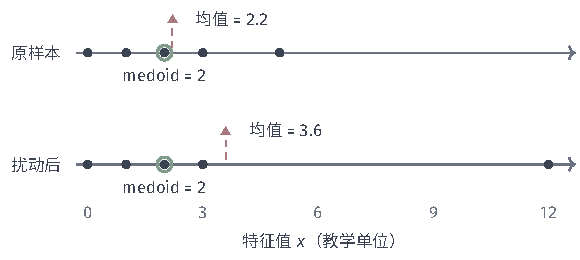
\includegraphics[width=98.231mm]{figures/04-classic-models/00-shared/tikz/clustering-medoid-robustness/figure.pdf}
  \caption{中心样本与均值对极端值的不同反应。固定 $K=1$，上方样本为 $\{0,1,2,3,5\}$，下方只把 5 改为 12；黑点为观测，圆圈标出绝对距离下的 medoid，三角形标出平方距离下的最优均值。}
 \label{fig:clustering-medoid-robustness}
\end{figure}

\subsubsection{参数学习}

\term{围绕中心样本划分}（Partitioning Around Medoids, PAM）通常包含 BUILD 初始化和 SWAP 改进。BUILD 贪心增加代表；SWAP 枚举每个当前代表 $m\in M$ 与每个非代表 $o\notin M$，计算
\[
 \Delta(m,o)=
 J\bigl((M\setminus\{m\})\cup\{o\}\bigr)-J(M).
\]
候选 $o$ 来自整个数据集，而不限于 $m$ 所在簇；每次交换后，所有样本都重新选择最近代表。只在固定簇内选取距离总和最小的样本，是另一种交替更新，不能替代 PAM 的 SWAP。

下面从随机代表开始，逐个评价完整交换邻域，以便核对$J(M)$与返回状态。代码省略BUILD初始化和距离差分缓存，适合作为目标及停止判据的教学实现。

\begin{codeblock}[language=Python,label={code:clustering-pam}]{PAM 的完整交换步骤}
import numpy as np

def pam_swap(D, K, seed=0, max_iter=100):
    n = len(D)
    if D.shape != (n, n) or not 1 <= K <= n or max_iter < 1:
        raise ValueError("invalid distance matrix, K, or max_iter")
    rng = np.random.default_rng(seed)
    medoids = rng.choice(n, K, replace=False)
    cost = D[:, medoids].min(1).sum()
    converged = False
    for _ in range(max_iter):
        best, best_cost = None, cost
        outside = np.setdiff1d(np.arange(n), medoids)
        for k in range(K):
            for o in outside:
                trial = medoids.copy()
                trial[k] = o
                value = D[:, trial].min(1).sum()
                if value < best_cost:
                    best, best_cost = trial, value
        if best is None:
            converged = True
            break
        medoids, cost = best, best_cost
    return D[:, medoids].argmin(1), medoids, converged
\end{codeblock}

完整扫描若未发现改进交换，代码返回\code{converged=True}，表明当前代表集合在单次交换邻域中局部最优。迭代上限先触发时，\code{converged=False}保留了尚未核完下一邻域的状态。严格下降使代表集合不重复，去掉上限并继续扫描时，有限候选集合保证最终停止。

预计算相异度矩阵占用$O(n^2)$存储，距离本身的计算还需另外计入。经典PAM缓存最近与次近代表，一轮完整交换通常按$O(K(n-K)^2)$量级分析。教学代码为每个候选重算$K$个距离列，额外重复了这些访问，因此成本更高。

\subsubsection{理论分析}

\paragraph{表达能力}
以欧氏距离作相异度时，K-medoids同样按最近代表分组，距离是否平方不改变两代表之间的等距边界。因此，前述内外同心圆不能由两个单一代表准确分开的限制仍然存在；换成真实样本并没有改变这一几何关系。改用编辑距离或图距离后，候选分组可以利用相应对象关系，但能否吻合目标要由该相异度决定，欧氏凸单元的结论也不再适用。

将代表限制在输入支持上，也可能使最小量化距离大于不受这一约束时的距离。以单位圆上均匀分布的输入和$K=1$为教学例，若允许任意欧氏位置作代表，圆心使期望距离达到最小值1；凸性与旋转对称性保证圆心最优。若代表必须是圆上的观测，则无论选择哪一点，期望距离都为
\[
 \frac1{2\pi}\int_0^{2\pi}2|\sin(\theta/2)|\,\mathrm d\theta
 =\frac4\pi.
\]
两者相差$4/\pi-1$。这种差异来自候选代表只能落在输入支持上，而非PAM没有搜索充分。若只允许代表来自输入支持的更小子集，候选空间进一步缩小，最小量化距离不会降低。



\paragraph{收敛性}
固定$K$时，样本代表集合至多有$\binom nK$种，因而最优集合存在。若每次交换都严格降低同一目标，已经访问的集合不能再次出现，至多接受$\binom nK-1$次交换后便会停止。PAM完整扫描没有改进时，得到的是单次交换意义下的局部最优；这个有限性上界很粗，也没有把局部解提升为全局解。

\paragraph{泛化性}
采用欧氏距离时，冻结代表后可以评价新样本的平均最近代表距离。

\begin{theorem}[K-medoids在有界欧氏输入下的期望量化风险界]
 \label{thm:clustering-medoids-risk}
设$D_n$独立同分布于$P$，$\lVert\bm X\rVert_2\leq r$，所有原型也在该球内。损失
$\ell_{\bm m}(\bm x)=\min_k\lVert\bm x-\bm m_k\rVert_2$
位于$[0,2r]$，原型最多移动$\epsilon$时损失最多改变$\epsilon$。沿用引理\ref{thm:clustering-cover-risk}的覆盖计算，得到
\begin{equation}
 \mathbb E_{D_n}R(\widehat{\bm m})
 \leq\inf_{\lVert\bm m_k\rVert_2\leq r}R(\bm m)
   +\frac{4r}{n}
   +4r\sqrt{\frac{Kd\log(1+2n)+\log2}{2n}}
   +\mathbb E_{D_n}e_n.
 \label{eq:clustering-medoids-risk}
\end{equation}
\end{theorem}

这里$e_n$按整个球中的原型计算，因此既含PAM等算法的搜索误差，也含代表只能来自样本的限制。即使完整求出最佳medoid，也不能直接令这个$e_n$为零。若用任意相异度，并预先固定$J$个候选代表、限制损失于$[0,M]$，则候选数至多为$J^K$，对应的超额风险界为
$2M\sqrt{[K\log J+\log(2/\delta)]/(2n)}+e_n$，概率至少为$1-\delta$。候选库由同一训练集生成时，不满足这个固定有限库的条件，需另作复杂度分析。

\subsubsection{优化计算能力}

完整交换邻域昂贵时，可以减少候选代表或减少检查的交换。Kaufman与Rousseeuw整理的CLARA在若干子样本上运行PAM，再用全体样本评价候选代表，以减少工作集；抽样未覆盖的小簇可能因此没有合适代表。Ng与Han在1994年提出的CLARANS把代表集合视为状态，随机抽取交换邻居，减少每轮扫描量\scite{clust-nghan1994}。前者限制本轮代表从哪里来，后者限制本轮搜索哪些交换，两者都需要评价近似搜索的损失。

重复计算也可以在保留交换目标的前提下减少。Schubert与Rousseeuw在2019年的FastPAM工作中复用不同被替换代表之间的计算，减少经典SWAP中随$K$重复的工作\scite{clust-schubert2019}。这种改进主要针对交换评价；关于$n$的距离访问和全量矩阵存储仍需计入，大样本的瓶颈可能继续来自这两部分。

\subsubsection{小结}

K-medoids以真实记录代表群组，可以解释典型对象，也能接收无法取均值的字符串等相异度输入。代表必须来自样本是一项实际约束，指定相异度又规定了哪些对象算作相近；极端值是否影响代表，需结合这两项选择判断。

搜索成本较高时，CLARA通过抽样缩小候选来源，CLARANS只检查部分交换，FastPAM则复用交换计算。前两者可能遗漏重要代表或改进机会，后一类加速仍需承担距离访问与存储。若连代表数也不想预先固定，第\ref{sec:clustering-affinity-propagation}节的AP提供另一种消息搜索路线，但同时改用偏好参数控制代表选择，不能当作PAM的等价加速。

\subsection{模型对比与总结}

原型方法共同用少量代表概括一批对象。K-means允许代表在向量空间中移动，平方欧氏距离使固定分组的最优代表可以直接取均值，更新成本较低。需要展示真实客户、典型文档或其他无法取均值的对象时，这个代表约束就不够：K-medoids改从观测中选代表，并允许采用指定相异度，代价是要搜索代表交换。表~\ref{tab:clustering-partition}比较这两个变化；采用真实代表也不自动带来鲁棒性，还需检查相异度对极端记录怎样计价。

\begin{table}[htbp]
 \small
 \begin{tabularx}{\linewidth}{@{}l>{\RaggedRight\arraybackslash}X>{\RaggedRight\arraybackslash}X@{}}
 \toprule
 比较项 & K-means & K-medoids\\
 \midrule
 代表 & 簇内均值向量 & 真实样本\\
 准则 & 平方欧氏距离和 & 指定相异度和\\
 优化步骤 & 最近中心与均值更新 & 代表交换与全局重分配\\
 主要成本 & 一轮 $O(nKd)$ & 完整交换搜索与距离访问\\
 典型用途 & 数值数据、向量量化 & 非数值对象、实例解释\\
 \bottomrule
 \end{tabularx}
 \caption{两类划分方法的比较。复杂度须与具体算法相联系；PAM 的成本不能套到所有 K-medoids 求解器。}
 \label{tab:clustering-partition}
\end{table}

围绕中心表示，损失和输出可以分别调整。K-medians把平方偏差换成绝对偏差，减弱少量极端记录对中心位置的牵动；FCM保留多个中心的软归属，表达边界过渡；核K-means改变比较坐标，使适当的非线性关系进入最近中心表示。前两者没有消除原空间单中心的形状限制，核方法也没有自动获得所需核。容量约束与二分层次则分别改变可行分配和输出粒度，回应了另一类使用要求。

数据规模主要影响怎样求解这些目标。Mini-Batch K-means用随机记录近似中心更新，CLARA限制代表搜索的工作集，CLARANS抽查交换机会；它们用近似换取较少访问。FastPAM则复用交换统计，减少同一搜索中的重复工作。选择时应同时核对失真、代表是否真实、重要小簇是否被抽样覆盖及资源预算，不能只把这些方法都归为“快速聚类”。

\section{基于邻域的聚类}
\label{sec:clustering-density}

环形、月牙形和弯曲条带中的样本可能远离同一中心，却能沿密集区域连接。密度方法据此把低密度分隔加入簇定义：一类方法寻找密集区域的连通分量，另一类寻找密度峰的吸引域。同一连通区域可以包含多个峰，因此两种定义会产生不同划分。

DBSCAN 直接用邻域计数判断密集程度，OPTICS 保留不同密度尺度的访问结构，Mean Shift 则沿核密度估计寻找驻点。噪声识别是前两者的显式输出；基本 Mean Shift 会为起点寻找归宿，并不自动拒绝孤立样本。

\subsection{DBSCAN}
\label{sec:clustering-dbscan}

考虑两条彼此分开的弯曲点带。沿同一条带相邻的样本很近，带的两个端点却可能很远；最近中心分配用到中心的距离，容易把一条带切开。若再有几个孤立点，K-means仍会把它们分进某个簇。DBSCAN（Density-Based Spatial Clustering of Applications with Noise）改用局部邻居的数量判断哪些位置足够密集，再沿相连的密集邻域扩展。只要两条带内部连通、带间没有密集路径，它们就可以各自形成一簇，孤立点则保留为噪声。Ester等在1996年提出了这一方法\scite{ester1996}。

原始DBSCAN面向带噪声的大型空间数据库，将任意形状的密集区域、参数知识需求和处理成本列为设计问题。邻域计数决定哪些点能扩展，连通搜索把它们组织成簇，无法归属的点保留噪声标记。这样，簇的数量和拒绝范围由局部密度关系共同确定。

\subsubsection{模型结构}

固定半径 $\varepsilon>0$ 和最小邻域样本数 $m=\mathrm{MinPts}$，定义索引邻域
\[
 N_\varepsilon(i)=
 \{j:\delta(\bm{x}_i,\bm{x}_j)\leq\varepsilon\}.
\]
本节假定相异度对称、样本到自身距离为零，并在邻域计数中包含自身。\term{核心点}（core point）满足 $|N_\varepsilon(i)|\geq m$；\term{边界点}（border point）不是核心点，但处在某个核心点的邻域内；既非核心也非边界的样本是\term{噪声点}（noise point）。

若 $i$ 是核心点且 $j\in N_\varepsilon(i)$，称 $j$ 从 $i$\term{直接密度可达}（directly density-reachable）。沿这样的有向关系组成有限链，就得到\term{密度可达}（density-reachable）：链上除终点外的点都须为核心点，终点可以是边界点。若存在一个核心点，使两个样本都从它密度可达，则称它们\term{密度相连}（density-connected）。

先只看核心点邻接图，可以清楚地区分扩展与吸收：距离不超过$\varepsilon$的核心点相连，每个连通分量提供一个簇的核心，再吸收相邻非核心点。边界点可能同时邻接多个分量；实际DBSCAN通常交给先访问它的簇，从而得到单一标签。图~\ref{fig:clustering-dbscan}展示了核心点继续扩展、边界点只被吸收的差别。

\begin{figure}[htbp]
  \centering
  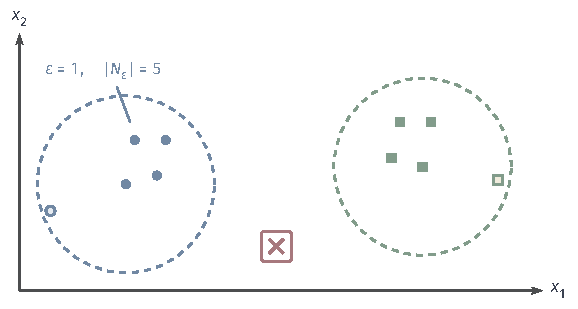
\includegraphics[width=97.850mm]{figures/04-classic-models/00-shared/tikz/clustering-dbscan/figure.pdf}
  \caption{DBSCAN的教学示意，取$\varepsilon=1$、$\mathrm{MinPts}=4$，计数包含自身。圆形和方形分别标识两个核心分量，颜色只作辅助；实心标记为核心点，浅色填充标记为边界点，红框叉号为噪声。虚线圆表示两个示例核心点的邻域；左侧标注直接给出邻域内计数，边界点不能继续扩展簇。}
 \label{fig:clustering-dbscan}
\end{figure}

\subsubsection{参数学习}

DBSCAN 的主要工作是查询邻域并搜索核心连通分量。代码~\ref{code:clustering-dbscan} 使用暴力距离查询，完整展示暂定噪声被重新吸收为边界点的情况。

\begin{codeblock}[language=Python,label={code:clustering-dbscan}]{DBSCAN 的邻域扩展}
import numpy as np
from collections import deque

def dbscan(X, eps, min_pts):
    X = np.asarray(X, dtype=float)
    if eps <= 0 or min_pts < 1:
        raise ValueError("invalid density parameters")
    labels = np.full(len(X), -1)  # -1 未访问，-2 噪声
    def neighbors(i):
        d2 = ((X - X[i]) ** 2).sum(1)
        return np.flatnonzero(d2 <= eps ** 2)
    cid = 0
    for i in range(len(X)):
        if labels[i] != -1:
            continue
        near = neighbors(i)
        if len(near) < min_pts:
            labels[i] = -2
            continue
        labels[i] = cid
        queue = deque(near)
        while queue:
            j = queue.popleft()
            if labels[j] == -2:
                labels[j] = cid
            if labels[j] != -1:
                continue
            labels[j] = cid
            near_j = neighbors(j)
            if len(near_j) >= min_pts:
                queue.extend(near_j)
        cid += 1
    return labels
\end{codeblock}

代码中每个样本至多查询一次邻域，队列则可能保存重复索引。暴力距离计算约需$O(n^2d)$运算。低维数据且邻域规模受控时，空间索引可使实践成本接近$O(n\log n)$；高维或大半径会增加访问量，最坏仍可达到平方级。预存全部邻域还可能占用$O(n^2)$内存。

参数选择可从第 $m$ 近邻距离的排序图入手，近邻计数约定应与是否包含自身一致。曲线的转折提示不同密度尺度，但未必存在清晰肘部。Schubert 等把 $\mathrm{MinPts}\approx 2d$ 作为平滑密度估计的经验起点，而不是一般最优值\scite{clust-schubert2017}。重复样本、噪声比例和有效维数都会影响合理的邻域大小与最小样本数。

\subsubsection{理论分析}

\paragraph{表达能力}
DBSCAN可以把一整条弯曲点带表示为一簇，因为同簇条件要求沿局部邻域连通，并不要求所有点都靠近一个中心。具体而言，假设目标划分中的每个点都有至少$m$个$\varepsilon$邻居，每个目标簇内部的$\varepsilon$邻接图连通，且不同目标簇之间的点距都大于$\varepsilon$。所有点此时都是核心点，核心图的连通分量恰与目标簇相同，DBSCAN便能完整表达该划分。条件中没有凸性要求，因此也适用于满足这些邻接条件的环形或月牙形样本。

同一机制也明确限定了哪些目标不能表达。两条点带之间若出现核心点组成的$\varepsilon$路径，DBSCAN就必须把它们合并，即使任务要求它们分开；若稀疏带上的点都不足$m$个邻居，它们就不能形成自己的核心簇。增大半径可以补足稀疏带的邻居，却可能同时连接稠密区域。这不是搜索精度不足，而是固定$(\varepsilon,m)$定义的候选分组与目标冲突。边界点还只能吸附到核心簇，若目标希望把一批彼此相近、却不邻接任何核心点的记录单独保留为簇，该参数下也无法做到。

\paragraph{收敛性}
DBSCAN的访问和扩展在有限样本上结束，其计算任务是搜索核心连通分量。由于这里没有连续参数的迭代优化，需要验证的是搜索是否完整，以及固定数据下哪些输出与访问顺序无关。

\begin{lemma}[DBSCAN 的核心点确定性]
 \label{thm:clustering-dbscan}
 固定数据、对称相异度和参数 $(\varepsilon,m)$，DBSCAN 输出的每个簇限制到核心点后，恰为核心点邻接图的一个连通分量。因此核心点划分与访问顺序无关，簇编号的置换除外。
\end{lemma}
\begin{proof}
在核心点集合上，距离不超过 $\varepsilon$ 的两点能相互直接密度到达。有限链的连通关系满足自反、对称和传递性，故图的连通分量就是核心点上密度相连关系的等价类。

从任一尚未访问的核心点扩展时，每发现一个核心邻居就加入它的邻域。沿路径长度归纳，该点所在连通分量中的每个核心点最终都会被访问。反过来，扩展过程只能经由核心点邻接边到达其他核心点，不能穿过非核心边界点连接两个分量。因此输出的核心集合既不遗漏本分量，也不包含其他分量，结论成立。
\end{proof}

定理固定了核心点划分。一个边界点若邻接多个核心分量，其单一归属仍由访问规则决定；簇编号和共享边界归属是两种不同的顺序影响。

\paragraph{泛化性}
DBSCAN的连通分量属于当前样本，加入新点可能改变核心计数并连接原先分开的分量。固定数据的搜索正确性因此不能直接给出新样本分组的期望风险。不过，核心判定本身可以先作为一个明确的总体任务来分析。

\begin{theorem}[DBSCAN在邻域质量间隔条件下的期望核心判定风险界]
 \label{thm:clustering-dbscan-core-risk}
设$D_n$独立同分布于$P$，新点独立于训练集。固定半径$\varepsilon$及质量阈值$t\in(0,1)$，记
$p_\varepsilon(\bm x)=P\{\delta(\bm x,\bm X)\leq\varepsilon\}$。
总体核心规则为$c_\star(\bm x)=\mathbf1\{p_\varepsilon(\bm x)\geq t\}$，训练后冻结的规则为
$\widehat c_n(\bm x)=\mathbf1\{n^{-1}\sum_i\mathbf1\{\delta(\bm x,\bm X_i)\leq\varepsilon\}\geq t\}$。
这里新点不计入训练邻居；$t$对应查询所用的计数阈值除以$n$。
若存在$\gamma>0$使$P\{|p_\varepsilon(\bm X)-t|\geq\gamma\}=1$，则新点的核心判定风险满足
\begin{equation}
 \mathbb E_{D_n}\!\left[
   P_{\bm X}\{\widehat c_n(\bm X)\ne c_\star(\bm X)\mid D_n\}
 \right]\leq2e^{-2n\gamma^2}.
 \label{eq:clustering-dbscan-core-risk}
\end{equation}
\end{theorem}

对每个固定查询$\bm x$，邻居指示量独立且均值为$p_\varepsilon(\bm x)$；越过判定阈值至少需要$\gamma$的计数偏差。Hoeffding界控制这一概率，再对独立新点积分，即得该式。没有统一间隔时，对任意$\gamma>0$仍有上界
$P\{|p_\varepsilon(\bm X)-t|<\gamma\}+2e^{-2n\gamma^2}$，阈值附近的概率质量成为额外误差。

这个结论只保证固定尺度下的核心判定，不保证连通簇与语义类别一致。要评价簇标签，必须另定总体簇、核心分量的匹配、新点分配以及冲突和拒绝规则；新增点重跑搜索也改变了学习器。OPTICS与HDBSCAN保留更多尺度，所选阈值若由同一批数据决定，也需另控制选择误差。

\subsubsection{小结}

DBSCAN由局部计数产生核心点，再以连通性形成簇，并显式保留噪声。它省去预设$K$，同时引入全局半径、计数阈值及距离选择。可恢复的形状由密度连通定义决定，高维查询和不同密度群组仍可能限制实际效果。

\subsection{OPTICS}
\label{sec:clustering-optics}

前述两条点带如果疏密不同，DBSCAN的单一半径就不容易选择：半径较小会拆散稀疏带，较大又可能把原本应分开的稠密区域连起来。反复换半径还会重复查询相似邻域。OPTICS（Ordering Points To Identify the Clustering Structure）在一次搜索中保存样本次序及进入相邻密集区域所需的距离，让我们事后查看不同尺度下的连接变化。Ankerst等在1999年提出的方法先给出这些记录，再由提取规则得到划分\scite{clust-ankerst1999}。

OPTICS把邻域计算与划分提取分开。DBSCAN在给定尺度后返回簇标签，OPTICS先保存访问次序和距离，供后续比较多种尺度。探索密度群组因而主要转为读取同一份结果，同时需要明确采用的提取规则。

\subsubsection{模型结构}

设搜索半径上限为 $\varepsilon_{\max}$。若样本 $i$ 在该半径内有至少 $m$ 个邻居，则其\term{核心距离}（core distance）为第 $m$ 近邻距离；否则记为 $+\infty$：
\[
 a_i=
 \begin{cases}
 \delta_{i,(m)},&|N_{\varepsilon_{\max}}(i)|\geq m,\\
 +\infty,&\text{其他情况}.
 \end{cases}
\]
由核心点 $i$ 到邻居 $j$ 的\term{可达距离}（reachability distance）定义为
\begin{equation}
 r(j\mid i)=\max\{a_i,\delta(\bm{x}_i,\bm{x}_j)\}.
 \label{eq:clustering-reachability}
\end{equation}
方向来自出发点的核心距离，因此通常 $r(j\mid i)\ne r(i\mid j)$。它表示在确保出发点足够密集的同时覆盖 $j$ 所需的半径。

OPTICS 为每个样本记录访问次序、核心距离和当前获得的最小可达距离。按访问次序画出可达距离形成\term{可达图}（reachability plot）；低谷通常对应容易从内部到达的密集区域，较高的过渡位置提示区域之间的分隔。

\subsubsection{参数学习}

从一个未处理点开始，算法输出该点并查询邻域。如果它是核心点，就用式~\eqref{eq:clustering-reachability} 更新未处理邻居的最小可达距离；优先队列每次取出当前可达距离最小的点，继续同样的过程。队列为空而仍有未处理点时，再开始一个新的搜索。这个过程是按可达距离优先的遍历，而不是普通先进先出的广度优先搜索。

给定 $\varepsilon'\leq\varepsilon_{\max}$，提取 DBSCAN 式结构时必须同时使用核心距离。沿排序扫描，若某点的记录可达距离大于 $\varepsilon'$，但核心距离不大于 $\varepsilon'$，它应开启一个新簇；若二者都大于阈值，才暂记为噪声；可达距离不大于阈值的点接续当前簇。只把水平线下的连续段当作簇，会漏掉可达距离很大、却负责开启新簇的核心点。不同提取规则对部分边界点的处理还可能与重新运行 DBSCAN 不同。

图~\ref{fig:clustering-optics-reachability} 将原始样本间距与可达图对应起来。中间一组样本较稀疏，形成的谷底较高；用 $\varepsilon'=0.35$ 提取时它们不构成核心簇，增大阈值才会纳入。次序 1、8、14 对应三次重新开始的搜索，其可达距离为无穷；次序 23 的孤立点也有无穷可达距离，但它的核心距离同样无穷，因而不能开启簇。

\begin{figure}[htbp]
  \centering
  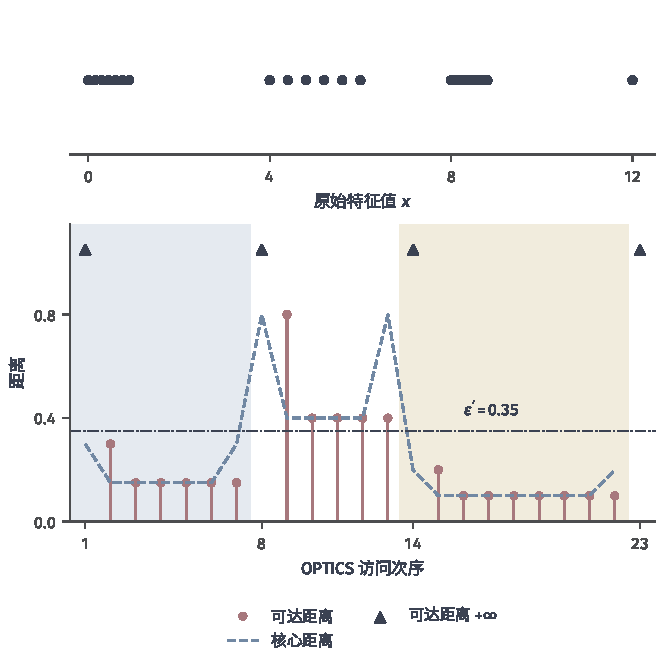
\includegraphics[width=105.412mm]{figures/04-classic-models/00-shared/matplotlib/clustering-optics-reachability/figure.pdf}
  \caption{固定一维教学数据上的OPTICS排序，取$\mathrm{MinPts}=3$（含自身）、$\varepsilon_{\max}=1.1$。三组样本的间距分别为$0.15$、$0.4$、$0.1$，另有$x=12$的孤立点。红色竖棒为可达距离，蓝色虚线为核心距离；蓝、黄底色标出两个低谷。无穷可达距离用顶部三角形表示，不能按其显示高度作数值比较；水平点划线展示阈值切割在本例中提取哪些低谷。}
 \label{fig:clustering-optics-reachability}
\end{figure}

低谷也可按相对陡降、陡升的$\xi$规则提取，并结合最小簇规模、前驱关系及嵌套处理。原始OPTICS已讨论陡峭区域，后续工作进一步构造密度层次。这里的自动提取减少人工读图，尺度和粒度仍由提取参数控制。

\subsubsection{理论分析}

\paragraph{表达能力}
OPTICS增加的是可供提取的密度尺度。对任意$\varepsilon'\leq\varepsilon_{\max}$，同时读取核心距离与可达距离，可以获得该尺度下的核心连通结构；若目标簇在某个这样的尺度满足前述DBSCAN邻接条件，它就在这份记录的可提取范围内。搜索上限之外的连接不会被记录，固定$m$下始终缺少邻居的小群体也不会因此变成核心簇。采用同一水平阈值提取时，疏密冲突依然存在；采用不同低谷的相对变化提取时，候选范围有所改变，但所需群组必须在相应低谷与边界中留下可区分的结构。记录多个尺度没有增加样本中缺失的分隔信息。



\paragraph{收敛性}
每个样本恰好进入输出次序一次，处理完$n$个样本后排序结束。若直接计算全部距离，邻域查询需要$O(n^2)$次距离计算；用二叉堆更新优先级，最坏可有$O(n^2)$次更新，每次代价$O(\log n)$。空间索引能减少一些数据上的搜索，但不改变高维或稠密邻域中的最坏情况。这里求解的是规定的访问次序及提取规则，不是迭代逼近某个全局最小损失。

\paragraph{泛化性}
\begin{theorem}[OPTICS预定有限尺度下的期望核心判定风险界]
对抽样前固定的$J$个半径及各自固定的质量阈值，若每个尺度的总体邻域质量与其阈值都相隔至少$\gamma>0$，可逐尺度应用定理\ref{thm:clustering-dbscan-core-risk}。令损失表示独立新点是否在至少一个尺度被误判为核心点，则并集界给出
\[
 \mathbb E_{D_n}R_{\mathrm{core}}\leq
       \min\{1,2J e^{-2n\gamma^2}\}.
\]
\end{theorem}

因此有限组预定尺度的核心判定可以同时推广到新点。可达图低谷的选择、簇标签的对应以及数据依赖的半径，仍需另行控制；这一结论不等于整条OPTICS层次的语义划分保证。

\subsubsection{优化表达能力}

OPTICS保存多个尺度的连接后，如何从这些尺度中选择群组仍需要规则。同一个尺度选择问题也可以用密度层次处理。Campello、Moulavi与Sander在2013年提出HDBSCAN框架，考察一个群组在多大尺度范围内持续存在，再据此提取簇\scite{clust-campello2013}。它另行构造层次，并非直接对OPTICS排序增加一个阈值。为了减小稀疏位置在较小尺度上过早连接的影响，它把两端点的核心距离$a_i,a_j$与原距离一起用于定义\term{互可达距离}（mutual reachability distance）：
\[
 \delta_{\mathrm{mr}}(i,j)
 =\max\{a_i,a_j,\delta(\bm{x}_i,\bm{x}_j)\}.
\]
在这一距离上构造最小生成树并形成密度层次，再按最小簇规模压缩层次、按跨尺度持续性选择簇，可以减轻单一$\varepsilon$的限制。代价是需要保存和处理层次，并明确最小簇规模及选择规则。

HDBSCAN的跨尺度持续性是层次中的簇选择量，评估抽样扰动还需要另外的统计协议。最小簇规模等参数继续控制输出，高维距离的区分度也需检验。密度路线将低密度分隔纳入簇定义；已有可信样本关系时，还可直接用图建立群组。

互可达距离使稀疏桥上的大核心距离成为连接下界，因而桥不会仅凭两点位置相近就在较小尺度接通。若目标群组分别在不同尺度形成并持续存在，它们可以出现在同一密度层次的不同分支中，随后由簇选择规则保留。若两个目标群组在所有保留尺度都没有分开，或目标小群体达不到最小簇规模，层次与持续性评分也不能创造这两个群组。最终选出的簇仍服从层次的包含关系，不能同时保留彼此交叉的两套分组。

\subsubsection{小结}

OPTICS把邻域搜索与划分提取分开，适合需要反复查看密度尺度的探索。它减少了更换阈值时的重复搜索，却增加了排序、优先队列和距离记录；$\varepsilon_{\max}$、$\mathrm{MinPts}$及提取规则继续决定哪些群组可以被读出。

HDBSCAN沿密度层次选择跨尺度持续的分支，回应的是怎样同时保留不同尺度的群组。它省去单一切割半径，仍需规定最小簇规模并承担层次构造成本。两种路线都要检查稀疏桥、小群体和高维距离，不能由多尺度记录本身推断语义分组已经正确。

\subsection{Mean Shift}
\label{sec:clustering-mean-shift}

密集路径与密度峰回答的是不同问题。两个聚集区域之间若有一条足够密集的连接带，DBSCAN可以把它们连为一簇；若希望把两处聚集峰分别识别出来，就需要考察密度在哪里达到局部高点。\term{均值漂移}（Mean Shift）先平滑估计密度，再把搜索点移向邻域样本的加权均值。在相应核条件下，这个移动方向与密度上升方向一致；从不同起点沿轨迹到达同一峰附近的样本可据此分组。平滑尺度会改变峰的数量，因此它也改变了所寻找的群组。

% 让历史段落自然接排，避免按整组引文高度提前截断正文。
Fukunaga与Hostetler在1975年从密度梯度估计出发，将局部均值偏移用于模式识别\scite{clust-fukunaga1975}。搜索先回答密度增加的方向，再据轨迹确定归宿，因此无需预先给出簇边界。

Cheng在1995年推广核与权重，讨论均值漂移、模态搜索和聚类之间的联系\scite{clust-cheng1995}。Comaniciu与Meer在2002年系统分析该方法，并展示特征空间和图像分割中的应用\scite{clust-comaniciu2002}。这些工作将密度上的移动规则与随后得到的簇分配联系起来，二者仍需分别规定停止与合并方式。

\subsubsection{模型结构}

以径向核估计未知密度。设 $h>0$ 为带宽，核函数为 $\mathcal{K}(\bm{u})=c_k k(\lVert\bm{u}\rVert_2^2)$，其中$c_k$是归一化常数，$k$是剖面函数（profile），规定核权重怎样随距离平方变化。则\term{核密度估计}（kernel density estimation, KDE）为
\begin{equation}
 \hat f(\bm{y})=\frac{c_k}{nh^d}
 \sum_{i=1}^n
 k\left(\frac{\lVert\bm{y}-\bm{x}_i\rVert_2^2}{h^2}\right).
 \label{eq:clustering-kde}
\end{equation}
可以从各样本出发在估计密度上搜索，把趋向同一模态的起点归为一簇。带宽决定平滑尺度，小带宽通常保留细节，大带宽通常合并邻近结构；模态数量的具体变化还依赖维数、核与样本分布。

\subsubsection{参数学习}

令 $g(u)=-k'(u)$，并记 $u_i(\bm{y})=\lVert\bm{y}-\bm{x}_i\rVert_2^2/h^2$。直接对式~\eqref{eq:clustering-kde} 求导可得
\[
 \nabla\hat f(\bm{y})=
 \frac{2c_k}{nh^{d+2}}
 \sum_i g(u_i(\bm{y}))(\bm{x}_i-\bm{y}).
\]
只要权重和为正，梯度便是正系数乘以\term{均值漂移向量}
\[
 \bm{m}(\bm{y})=
 \frac{\sum_i g(u_i(\bm{y}))\bm{x}_i}
      {\sum_i g(u_i(\bm{y}))}-\bm{y}.
\]
因此采用下列自适应步长的梯度方向更新：
\begin{equation}
 \bm{y}^{(t+1)}=
 \frac{\sum_i w_i^{(t)}\bm{x}_i}{\sum_i w_i^{(t)}},
 \qquad w_i^{(t)}=g(u_i(\bm{y}^{(t)})).
 \label{eq:clustering-mean-shift}
\end{equation}
权重来自一元剖面函数的负导数$g$，其自变量是距离平方。高斯剖面$k(u)=\exp(-u/2)$给出与高斯权重成比例的$g$，Epanechnikov剖面$(1-u)_+$在支撑内部给出常数权重，边界按分段规则处理。

式~\eqref{eq:clustering-mean-shift}与第\ref{sec:regression-nadaraya-watson}节的Nadaraya--Watson回归都计算核加权平均。Mean Shift平均输入位置，更新搜索点；核回归平均响应，预测条件均值。相同的平均运算承担不同的估计任务。

图~\ref{fig:clustering-mean-shift-modes}固定同一组一维样本，两个起点沿式~\eqref{eq:clustering-mean-shift}分别向左右峰移动，靠近驻点时位移减小。灰线改用更大带宽，两个峰合为一个峰。起点决定从哪里搜索，带宽改变估计密度及可到达的模态，两项选择因而影响不同的对象。

\begin{figure}[htbp]
  \centering
  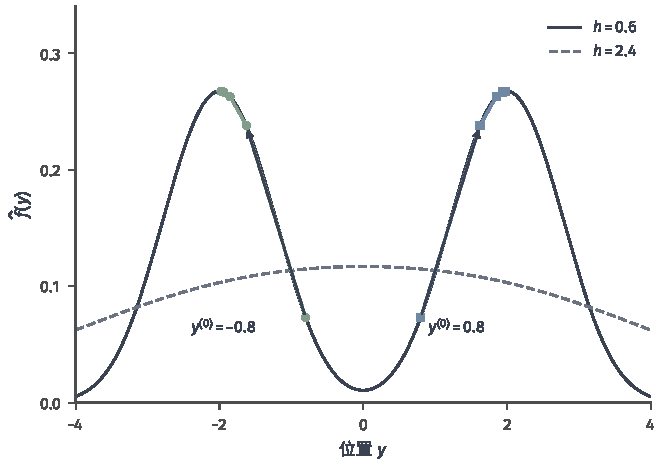
\includegraphics[width=105.412mm]{figures/04-classic-models/00-shared/matplotlib/clustering-mean-shift-modes/figure.pdf}
  \caption{Mean Shift 的密度爬升与带宽效应。左右各有三个样本，位置为 $-2.5,-2,-1.5$ 和 $1.5,2,2.5$，均采用高斯核。彩色标记给出带宽 $h=0.6$ 时从 $\pm0.8$ 出发的初始位置和四次更新，箭头指示第一次移动；灰色虚线对应 $h=2.4$，轨迹在黑色实线上计算。}
 \label{fig:clustering-mean-shift-modes}
\end{figure}

\begin{codeblock}[language=Python,label={code:clustering-mean-shift}]{高斯 Mean Shift 的起点更新}
import numpy as np

def mean_shift_positions(X, h, max_iter=300, tol=1e-4):
    X = np.asarray(X, dtype=float)
    if h <= 0:
        raise ValueError("h must be positive")
    Y = X.copy()
    for _ in range(max_iter):
        d2 = ((Y[:, None] - X[None]) ** 2).sum(2)
        log_w = -d2 / (2 * h * h)
        log_w -= log_w.max(1, keepdims=True)
        W = np.exp(log_w)
        new = (W @ X) / W.sum(1, keepdims=True)
        step = np.linalg.norm(new - Y, axis=1).max()
        Y = new
        if step <= tol:
            break
    return Y
\end{codeblock}

代码返回最终位置。得到簇标签还需合并相近终点，例如构造距离不超过$\rho$的终点图并取连通分量；$\rho=h/2$可作教学起点。这个合并阈值与更新容差用途不同，连通规则可能沿一串近终点把不同模态接在一起，需单独检查。

全部$n$个起点的一轮精确更新约需$O(n^2d)$运算。高斯核覆盖所有样本，因此截断邻域或近似近邻改变了精确更新。大数据实现可分块、减少起点或改用有限支撑核，并分别核对计算节省与位置误差。

\subsubsection{理论分析}

\paragraph{表达能力}
Mean Shift所拟合的是核平滑后的密度，输出则由其峰及吸引域确定。带宽对目标分组的影响可以用两个一维观测$-a,a$准确说明，其中$a>0$。取高斯核，两观测产生的密度与
\[
 e^{-(y-a)^2/(2h^2)}+e^{-(y+a)^2/(2h^2)}
\]
成比例，驻点满足$y=a\tanh(ay/h^2)$。在正半轴，右侧函数先以斜率$a^2/h^2$增长，随后斜率不断减小。若$a\leq h$，它不能再次越过直线$y$，唯一峰位于0；若$a>h$，两者在正半轴另有一个交点，负半轴对称地再有一个，0成为局部谷底，两侧各有一个峰。因而希望分别表示两处聚集时，过大的带宽会使两个峰在候选密度中消失，即使驻点求解完全准确也不能找回它们。

峰的吸引域也不等于密度连通簇。两个峰之间存在密集桥时，DBSCAN可以沿桥合并，Mean Shift仍可能按不同上升归宿分组；反过来，同一语义群体具有多个峰时，也可能被拆开。判断表达是否充分，需要先确认目标是平滑尺度下的模态分组，还是另一种关系；终点合并阈值还会进一步改变可保留的峰。

\paragraph{收敛性}
Mean Shift的上升不等式控制密度值，位置收敛还需排除轨迹在多个聚点之间移动。步长平方可和只说明步长趋零，后续研究指出了将它直接推为Cauchy性的缺口\scite{clust-aliyari2015}。下面用紧性、连续性和有限固定点补足这一步。

\begin{theorem}[Mean Shift在高斯核下的密度上升与条件收敛]
 \label{thm:clustering-mean-shift}
 设 $k$ 非负、凸、非增且可微，$k(0)<\infty$，迭代中权重和始终为正。则式~\eqref{eq:clustering-mean-shift} 产生的密度值单调不减且收敛。若进一步假设 $g=-k'$ 连续且严格为正，样本凸包内的固定点只有有限个，则位置序列也收敛，极限为 $\hat f$ 的驻点。
\end{theorem}
\begin{proof}
简记 $\bm{y}=\bm{y}^{(t)}$、$\bm{y}'=\bm{y}^{(t+1)}$。由凸性，
\[
 k(u_i(\bm{y}'))-k(u_i(\bm{y}))
 \geq g(u_i(\bm{y}))
       \bigl(u_i(\bm{y})-u_i(\bm{y}')\bigr).
\]
令 $w_i=g(u_i(\bm{y}))$、$s=\sum_iw_i$。由于 $\bm{y}'$ 是加权均值，展开平方后交叉项为零，得到
\[
 \sum_iw_i\bigl(
 \lVert\bm{y}-\bm{x}_i\rVert_2^2
 -\lVert\bm{y}'-\bm{x}_i\rVert_2^2\bigr)
 =s\lVert\bm{y}'-\bm{y}\rVert_2^2.
\]
所以
\begin{equation}
 \hat f(\bm{y}')-\hat f(\bm{y})
 \geq\frac{c_k s}{nh^{d+2}}
       \lVert\bm{y}'-\bm{y}\rVert_2^2\geq0.
 \label{eq:clustering-mean-shift-ascent}
\end{equation}
又有 $\hat f(\bm{y})\leq c_k k(0)/h^d$，故密度值收敛。

在附加条件下，第一次更新后所有位置均在有限样本的紧凸包内。距离平方因此有界，而连续正函数 $g$ 在相应紧区间上有正下界，故 $s$ 也有统一正下界。对式~\eqref{eq:clustering-mean-shift-ascent} 求和，得到步长平方可和，特别地，$\lVert\bm{y}^{(t+1)}-\bm{y}^{(t)}\rVert_2\to0$。

记连续更新映射为 $T$。任取收敛子列 $\bm{y}^{(t_j)}\to\bm{y}^\ast$，步长趋零与连续性给出 $T(\bm{y}^\ast)=\bm{y}^\ast$，所以每个聚点都是固定点。固定点有限，取彼此不相交的小球包围它们；序列最终必在这些小球的并集中，否则紧性会产生球外聚点。步长最终小于球之间的间隙，故序列不能再从一个球跳到另一个球。任意缩小球半径，便知它只能趋向其中一个固定点。梯度公式最后给出 $\nabla\hat f(\bm{y}^\ast)=\bm{0}$。
\end{proof}

位置收敛由紧性、连续性及有限固定点共同支持，平方可和用于先证明步长趋零。极限是驻点，特殊起点可能停在鞍点；解释为密度峰还需检查局部形状。Epanechnikov核的分段边界和零权重不满足第二部分的全部条件，需另作分析。

\paragraph{泛化性}
Mean Shift搜索的是训练样本构成的密度$\widehat f_h$。要判断这一对象是否接近总体，先评价密度估计误差，再考虑峰与吸引域；搜索当前密度的上升性不控制这项统计误差。

\begin{theorem}[Mean Shift所用KDE在二阶光滑密度下的期望估计误差]
 \label{thm:clustering-kde-risk}
设独立同分布观测的密度$f$定义在$\mathbb R^d$上，$f$二阶连续可微且平方可积，并满足
$\int\lVert\nabla^2f(\bm x)\rVert_F^2\,\mathrm d\bm x\leq A^2$。取非负积分为一的核$\psi$，满足
\[
 \begin{gathered}
 \int\bm u\psi(\bm u)\,\mathrm d\bm u=\bm0,\\
 m_2=\int\lVert\bm u\rVert_2^2\psi(\bm u)\,\mathrm d\bm u<\infty,
 \qquad\lVert\psi\rVert_{L^2}<\infty.
 \end{gathered}
\]
对带宽$h>0$的KDE
\[
 \widehat f_h(\bm x)=(nh^d)^{-1}\sum_i\psi((\bm x-\bm X_i)/h),
\]
有
\begin{equation}
 \mathbb E_{D_n}\lVert\widehat f_h-f\rVert_{L^2}^2
 \leq\frac{A^2m_2^2h^4}{4}
      +\frac{\lVert\psi\rVert_{L^2}^2}{nh^d}.
 \label{eq:clustering-kde-risk}
\end{equation}
\end{theorem}

证明将误差分成平方偏差与积分方差。二阶Taylor余项及核的一阶矩为零给出
$\lVert\mathbb E\widehat f_h-f\rVert_{L^2}\leq Am_2h^2/2$；独立样本使积分方差至多为$\lVert\psi\rVert_{L^2}^2/(nh^d)$。取$h$与$n^{-1/(d+4)}$同阶，两项合为$O(n^{-4/(d+4)})$。这是训练抽样平均的密度估计风险，适用于使用同一KDE的Mean Shift与DENCLUE。

该风险趋零仍未给出峰位置或新点簇标签的误差界。很平的峰可能随很小的密度扰动移动，吸引域边界附近的新点也可能改换归宿；从密度风险推进到这两个任务，需要控制导数误差、峰的曲率和边界附近的概率质量。带宽选择应对应所评价的任务。

\subsubsection{支持低密度背景排除场景}

Mean Shift按搜索归宿分组时，还需决定如何对待密度很低的驻点。沿同一平滑密度思路，Hinneburg与Keim在1998年提出DENCLUE，把各样本的影响函数相加，以密度阈值排除弱峰，再用吸引点及其连通关系组织簇\scite{clust-hinneburg1998}。网格减少密度计算需要访问的对象，同时要控制省略远处贡献的近似。它另行规定密度搜索、峰的保留与计算组织，高维估计是否可靠仍取决于样本量、表示和核尺度。

若任务把低于$t$的密度区域视为背景，DENCLUE的阈值允许这部分对象不形成独立簇，比基本Mean Shift保留所有模态更接近该目标。它所保留的区域仍属于指定影响函数产生的平滑密度：两个目标群组之间若在这一密度的$t$水平以上连通，按密度连接合并时就不能把它们分开；一个目标群组的最高密度若低于$t$，则会被整体排除。降低$t$可以保留弱群组，也可能把背景连接一并纳入。

\subsubsection{小结}

Mean Shift适合寻找平滑密度中的聚集峰，以局部加权均值推进搜索，再按归宿组织样本。簇数取决于带宽、起点和终点合并；图像分割与跟踪可以利用这种聚集机制，但弱峰、平坦驻点和反复邻域访问都需要处理。

若背景中的弱峰不应独立成簇，DENCLUE用阈值规定保留哪些吸引点，并允许根据密度连接合并它们。阈值会同时改变弱群体与背景的取舍，网格近似则改变密度计算预算。这条路线与基本模态归宿分组的区别在簇提取规则，不能仅根据两者都使用密度爬升就认为输出相同。

\subsection{模型对比与总结}

密度方法有两种不同的群组定义。DBSCAN把满足计数条件的核心点沿邻域连接，再接纳边界点；同一条弯曲的密集路径可以成为一簇，低密度对象则作为噪声。Mean Shift先估计平滑密度，把到达同一峰的搜索轨迹归为一组。两处密度峰之间即使有足够密集的连接带，也可能在DBSCAN中合为一簇、在Mean Shift中分成两组。前者保留连通区域，后者区分聚集归宿，选择首先取决于要解释哪一种结构。

在连通路线中，DBSCAN的单一半径难以同时照顾稠密簇和稀疏簇：照顾稀疏簇所需的大半径也可能接通稠密簇之间的桥。OPTICS保存可达排序及距离，把邻域搜索与尺度提取分开，便于观察哪些群组在不同尺度出现；它仍需提取规则，使用同一水平阈值时也仍会遇到疏密冲突。HDBSCAN另建互可达距离的层次，再根据最小簇规模及跨尺度持续性选分支，使不同群组可以在不同密度尺度上保留。它与OPTICS共享对多尺度结构的关注，层次构造和选择准则则不同。

在模态路线中，带宽决定Mean Shift看到的是许多细峰还是少数宽峰。若低密度背景中的弱峰不应独立成簇，DENCLUE通过密度阈值筛选吸引点，并按密度连接组织群组；它同时改变了峰的保留和合并方式。阈值降低会保留更多弱群体，也可能纳入背景连接，因而不能只把它看成更快的Mean Shift。

这些调整分别回应单一尺度、弱峰和连接规则的问题，没有消除表示与距离选择的责任。比较时应检查目标小群体是否被保留、桥接是否符合用途，以及查询、密度估计和层次提取的成本；同一二维散点图上的相近划分，可能来自不同的簇定义。

\section{基于图的聚类}
\label{sec:clustering-graph}

社交连接、文档相似度和像素邻接可以直接表示为加权图。图聚类将样本作为顶点、相似程度作为边权，寻找内部连接较强而外部连接较弱的群组。向量距离也可用于建图；边权和邻域规则因此继续决定所保留的相似关系。

仅最小化切边权重，可能轻易切下一个连接少的小块。对簇规模或连接体积作归一化，可以比较“割断多少联系”与“簇原来拥有多少联系”。谱聚类再把这一离散搜索松弛为特征向量求解。

\subsection{谱聚类}
\label{sec:clustering-spectral}

弯曲点带还可以用图来表示：只给相近样本连边，同一条带内有许多连接，两条带之间只有很少连接。分组便转为切断较少的跨组联系。不过，直接寻找最优图划分需要搜索组合众多的标签方案。\term{谱聚类}（spectral clustering）先将离散标签放松为连续数值，用图拉普拉斯的特征向量求取低成本的连续表示，再在该表示上划分顶点。它改变了中心方法所使用的坐标，但分组结果仍取决于图是否保留了可信的相似关系。von Luxburg的教程整理了图构造、归一化及适用条件\scite{clust-luxburg2007}。

第\ref{sec:dim-le}节的拉普拉斯特征映射共享建图与低频谱表示，直接输出连续坐标；谱聚类还需要离散分配。下面以归一化割及多簇谱算法说明这两步怎样衔接。

Donath与Hoffman在1973年用谱信息给图划分代价建立下界，将组合搜索与可计算特征值联系起来\scite{clust-donath1973}。Shi与Malik进一步用像素相似关系建立归一化割，相关会议和期刊论文分别发表于1997年和2000年\scite{clust-shi2000}。Ng、Jordan与Weiss在2001年会议提出多簇谱嵌入与行归一化，论文集于2002年出版\scite{clust-ng2002}。这些工作分别解释了图目标、连续表示及离散化的连接。

\subsubsection{模型结构}

设无向图的非负对称权重矩阵为 $\bm{W}\in\mathbb{R}^{n\times n}$，通常令 $w_{i,i}=0$。向量样本可用高斯相似度 $\exp(-\lVert\bm{x}_i-\bm{x}_j\rVert_2^2/(2\sigma^2))$ 构造边；近邻图则保留部分局部关系。单向近邻关系未必对称，必须明确采用并集对称化还是互近邻规则。

定义顶点度 $d_i=\sum_jw_{i,j}$、度矩阵 $\bm{D}=\operatorname{diag}(d_1,\ldots,d_n)$，以及三种拉普拉斯：
\begin{align}
 \bm{L}&=\bm{D}-\bm{W},\nonumber\\
 \bm{L}_{\mathrm{sym}}
 &=\bm{I}-\bm{D}^{-1/2}\bm{W}\bm{D}^{-1/2},\nonumber\\
 \bm{L}_{\mathrm{rw}}
 &=\bm{I}-\bm{D}^{-1}\bm{W}.
 \label{eq:clustering-laplacians}
\end{align}
归一化所用逆度数要求$d_i>0$，因此先单独处理孤立顶点。$\bm{L}_{\mathrm{rw}}$ 一般不对称，但与 $\bm{L}_{\mathrm{sym}}$ 相似，因而有相同的实特征值。对任意 $\bm{v}\in\mathbb{R}^n$，
\begin{equation}
 \bm{v}^{\top}\bm{L}\bm{v}
 =\frac12\sum_{i,j}w_{i,j}(v_i-v_j)^2\geq0.
 \label{eq:clustering-laplacian-form}
\end{equation}
所以 $\bm{L}$ 半正定，且 $\bm{L}\bm{1}=\bm{0}$；零特征值的重数等于连通分量数，图连通时才为单重。

归一化还具有随机游走解释。转移矩阵 $\bm{P}=\bm{D}^{-1}\bm{W}$ 让游走者按边权比例选择下一顶点，且 $\bm{L}_{\mathrm{rw}}=\bm{I}-\bm{P}$。从一个簇出发，若内部连接强而外部连接弱，游走就倾向在簇中停留较久；Meilă 与 Shi 据此研究了聚类的随机游走视角\scite{clust-meila2001}。

设 $\operatorname{cut}(A,\bar A)=\sum_{i\in A,j\notin A}w_{i,j}$，$\operatorname{vol}(A)=\sum_{i\in A}d_i$。\term{归一化割}（normalized cut, NCut）定义为
\begin{equation}
 \operatorname{NCut}(\mathcal{P})
 =\sum_{k=1}^K
 \frac{\operatorname{cut}(C_k,\bar C_k)}
      {\operatorname{vol}(C_k)}.
 \label{eq:clustering-ncut}
\end{equation}
它比较切边与簇内外连接体积，减轻小簇的偏好；同体积的簇可以含不同样本数\scite{clust-shi2000}。\term{比率割}（RatioCut）则把分母换成 $|C_k|$，对应未归一化拉普拉斯的松弛。

\subsubsection{参数学习}

为把 NCut 改写成矩阵目标，定义 $\bm{F}\in\mathbb{R}^{n\times K}$，其中
\[
 f_{i,k}=
 \begin{cases}
  1/\sqrt{\operatorname{vol}(C_k)},&i\in C_k,\\
  0,&i\notin C_k.
 \end{cases}
\]
簇互不相交给出 $\bm{F}^{\top}\bm{D}\bm{F}=\bm{I}_K$。由式~\eqref{eq:clustering-laplacian-form}，第 $k$ 列的二次型恰为第 $k$ 项归一化割，故目标为 $\operatorname{tr}(\bm{F}^{\top}\bm{L}\bm{F})$。

困难在于每行只允许一个特定的非零值。去掉这一离散约束，令 $\bm{H}=\bm{D}^{1/2}\bm{F}$，得到
\begin{equation}
 \min_{\bm{H}^{\top}\bm{H}=\bm{I}_K}
 \operatorname{tr}(\bm{H}^{\top}
                   \bm{L}_{\mathrm{sym}}\bm{H}).
 \label{eq:clustering-spectral-relaxation}
\end{equation}
Shi--Malik 方法也可写为广义特征问题 $\bm{L}\bm{f}=\lambda\bm{D}\bm{f}$，与归一化变换相联系\scite{clust-shi2000}。取 $\bm{L}_{\mathrm{sym}}$ 最小的 $K$ 个特征值对应的特征向量，即得到式~\eqref{eq:clustering-spectral-relaxation} 的最优解；下文说明这一连续最优值及其唯一性条件。

连续解还需离散化。\term{NJW 算法}把 $\bm{H}$ 每一行归一化到单位长度，再对行向量运行 K-means\scite{clust-ng2002}。若图恰有 $K$ 个连通分量，理想谱空间中每个分量对应同一方向；行归一化消除度数造成的长度差异，图~\ref{fig:clustering-spectral} 展示了这一解释。连接较弱的实际图中，这只是近似结构。

\Needspace{62mm}
\begin{figure}[htbp]
  \centering
  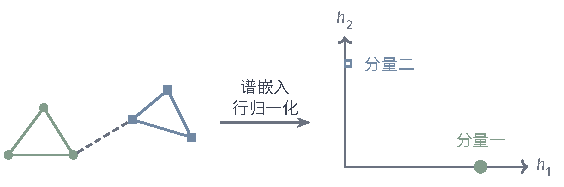
\includegraphics[width=95.564mm]{figures/04-classic-models/00-shared/tikz/clustering-spectral/figure.pdf}
  \caption{谱聚类的理想情形：圆形与方形分别标识两个互不连接的分量，颜色只作辅助；在归一化谱空间中，两个分量分别落到两个方向。细虚线表示实际数据中可能存在的弱连接；加入这些连接后，谱坐标通常形成近似群组。}
 \label{fig:clustering-spectral}
\end{figure}

\begin{codeblock}[language=Python,label={code:clustering-spectral}]{给定相似度矩阵的 NJW 算法}
import numpy as np
from scipy.linalg import eigh

def spectral_clustering(W, K):
    W = np.asarray(W, dtype=float)
    n = len(W)
    if W.shape != (n, n) or not 1 <= K <= n:
        raise ValueError("invalid shape or K")
    if (W < 0).any() or not np.allclose(W, W.T):
        raise ValueError("W must be nonnegative and symmetric")
    degree = W.sum(1)
    if (degree <= 0).any():
        raise ValueError("handle isolated vertices first")
    inv = 1 / np.sqrt(degree)
    L = np.eye(n) - inv[:, None] * W * inv[None, :]
    _, H = eigh(L, subset_by_index=[0, K - 1])
    length = np.linalg.norm(H, axis=1)
    if (length == 0).any():
        raise ValueError("zero embedding row")
    labels, _ = kmeans(H / length[:, None], K)
    return labels
\end{codeblock}

代码复用代码~\ref{code:clustering-kmeans}的K-means函数，处理能放入内存的稠密矩阵。图的连通分量数超过$K$时，所选零特征子空间可能含零行，也可能将多个分量任意合并。应先确定各连通分量是否需要独立输出，再选择谱子空间与分配策略。

稠密建图约需$O(n^2d)$距离运算和$O(n^2)$存储，完整特征分解约需$O(n^3)$。只求部分特征向量时，可用Lanczos或LOBPCG，矩阵乘法成本可按稀疏边数计算；迭代总成本还受特征间隙、精度和迭代次数影响。大规模实现可结合近邻图或Nyström近似，并核对它们对谱表示的误差。

\subsubsection{理论分析}

\paragraph{表达能力}
离散NCut的候选是图顶点的$K$簇划分，并不要求每簇在原向量空间中凸。对两条没有跨带边、各自内部连通的弯曲点带，取$K=2$，按点带划分的NCut为零，已达到非负目标的最小值。这比原空间两个Voronoi单元更能表达“一条带一簇”。

有跨组边时，目标划分仍在离散候选中，但不一定是NCut最优。若两个语义群组之间有很强连接，而另一个较小切口的相对边权更低，图割就会偏向后者。谱方法对非凸形状的收益因此来自可信的局部连接，而非低维谱坐标无条件地恢复了语义类别。

\paragraph{收敛性}
谱聚类的求解分为特征子空间计算与离散分组。前一阶段要找到最小的$K$个特征值及其子空间，并达到残差精度；后一阶段的K-means另有初始化与停止条件。下面先确定连续松弛的全局最优值，随后再说明它与离散图割质量的关系。

在式~\eqref{eq:clustering-spectral-relaxation}中，令$\bm B=\bm L_{\mathrm{sym}}$，并取$1\leq K\leq n$。将这个实对称谱算子的特征值按升序记为$\lambda_1\leq\cdots\leq\lambda_n$，对应标准正交特征向量为$\bm u_1,\ldots,\bm u_n$。正交列约束下的连续松弛最优值为
\[
 \min_{\bm H^\top\bm H=\bm I_K}
 \operatorname{tr}(\bm H^\top\bm B\bm H)
 =\sum_{k=1}^K\lambda_k.
\]
取$\bm H=[\bm u_1,\ldots,\bm u_K]$即可达到该值。若$K<n$且$\lambda_K<\lambda_{K+1}$，最优列空间唯一，但其中的正交基仍可右乘正交矩阵（参考\BookTheoremRef{thm:matrix-analysis-trace-minimum}{卷1《数学准备：计算、分析与几何》第5章“线性空间”第5.5.4节“秩约束下的矩阵逼近”}）。这个结论确定的是连续子空间；把它转换成离散簇标签，还需要前述离散化步骤。

在理想图上，谱松弛与离散化可以保留原图割目标：若图恰有$K$个连通分量且所有顶点度为正，零特征空间由各分量的度加权指示向量张成。行归一化后，同一分量的行完全相同，不同分量的行对应不同正交方向，因而全局最优的$K$-means离散化可给出零失真并恢复这$K$个分量。

即使特征向量计算准确，也只说明得到了该图的连续最优解；错误边权改变了目标，松弛和离散化还可能留下额外差异。

图割质量与谱量之间还存在 Cheeger 型联系。对连通、非负无向图，定义\term{电导}（conductance）
\[
 \phi(S)=
 \frac{\operatorname{cut}(S,\bar S)}
 {\min\{\operatorname{vol}(S),\operatorname{vol}(\bar S)\}},
 \qquad h_G=\min_{\varnothing\ne S\ne V}\phi(S).
\]
若 $\lambda_2$ 是 $\bm{L}_{\mathrm{sym}}$ 的第二小特征值，则
\begin{equation}
 \frac{\lambda_2}{2}\leq h_G\leq\sqrt{2\lambda_2}.
 \label{eq:clustering-cheeger}
\end{equation}
图上的这类不等式把低频特征向量与稀疏切割联系起来，标准谱图论教材给出了证明及其与流形版本的关系\scite{clust-chung1997}。

这里$h_G$最小化电导，NCut则对两个方向分别按体积归一；二者的关系需由分母比较得到。二分情形满足 $\phi(S)\leq\operatorname{NCut}(S,\bar S)\leq2\phi(S)$。若 $\bm{u}$ 是 $\bm{L}_{\mathrm{sym}}$ 的第二特征向量，则
\[
 \bm{f}=\bm{D}^{-1/2}\bm{u},
 \qquad
 \bm{L}\bm{f}=\lambda_2\bm{D}\bm{f},
 \qquad
 \bm{L}_{\mathrm{rw}}\bm{f}=\lambda_2\bm{f}.
\]
因此，Cheeger sweep 应按 $f_i=u_i/\sqrt{d_i}$ 排序并扫描阈值；若直接求广义特征问题或随机游走拉普拉斯，排序坐标就是其特征向量 $\bm{f}$。只有各顶点度数相同时，按 $\bm{u}$ 与按 $\bm{f}$ 排序才必然相同。这一保证对应二分的阈值扫描；多簇NJW加K-means使用另一离散化规则，其图割质量需另行分析。

\paragraph{泛化性}
谱聚类的训练输出是给定图的划分，先前的Cheeger界可以解释成该图上的关系损失。设图连通、权重对称非负，$S$为非空真子集，$I$在$S$内按$d_i/\operatorname{vol}(S)$抽取，再按$w_{ij}/d_i$走一步到$J$。离开$S$的概率为
\[
 P(J\notin S\mid I\in S)
 =\frac{\operatorname{cut}(S,\bar S)}{\operatorname{vol}(S)}.
\]
从$\bar S$开始的离开概率同理；二者之和恰为$\operatorname{NCut}(S,\bar S)$。按第二特征向量的正确归一化坐标作阈值扫描，Cheeger结论保证存在输出$\widehat S$使
\begin{equation}
 R_G(\widehat S):=\operatorname{NCut}(\widehat S,\bar{\widehat S})
 \leq2\sqrt{2\lambda_2}.
 \label{eq:clustering-spectral-graph-risk}
\end{equation}
这是冻结图后，对图上随机游走的期望跨簇损失；它没有对新的独立对象给出风险界。多簇NJW加K-means也不能直接套用这个二分扫描结论。

总体分布上的评价还需指定建图制度与新点分配。固定相似核时，经验谱对象可以向总体积分算子收敛\scite{clust-luxburg2008}，但算子或子空间一致性尚未给出新点分组损失，离散化、簇匹配和边界处的概率质量仍需控制。带宽随$n$改变的流形极限则有另一组采样、带宽及归一化条件。本节的明确风险保证止于式\eqref{eq:clustering-spectral-graph-risk}所规定的有限图任务。

\subsubsection{支持样本对关系监督场景}

如果已知某两条记录应当同簇，或另一对记录应当异簇，就可以让这些关系改变谱聚类所用的图。Kamvar、Klein与Manning的Spectral Learning研究了将监督信息纳入谱表示；一种直接做法是提高应同簇样本对的边权、降低应异簇样本对的边权，再对修改后的非负对称图求谱表示\scite{clust-kamvar2003}。

边权调整改变谱偏好，最终分配仍由整张图和离散化决定。即使删除应异簇样本对之间的边，两端也可能通过其他强边共簇。修改后的非负对称图可按其新拉普拉斯分析，但谱间隙、连接及统计条件需重新核对。关系传播还能扩展局部监督，同时可能扩散错误信号。

\subsubsection{小结}

谱聚类以关系图保留非凸连接结构，用特征分解求连续松弛，再通过离散化形成簇。图构造与最后分配共同影响结果。特征值间隙可作为探索$K$的线索，解释时还需排查噪声、弱连接与孤立分量造成的间隙。

\subsection{代表选择与消息传播}
\label{sec:clustering-affinity-propagation}

谱聚类希望划分连接较强的群组。如果任务更重视“每组由哪条记录代表”，就可以回到真实样本代表的思路。K-medoids需要预先指定代表数，Frey与Dueck在2007年提出的\term{近邻传播}（Affinity Propagation, AP）则让每个样本都成为潜在代表，通过两类消息协调选择。

\subsubsection{模型结构}

适合度描述样本对一个候选代表的支持，可用度汇总该候选能否作为代表的其他支持；对代表本身设置的偏好间接控制代表数。

\subsubsection{参数学习}

给定相似度$s(i,k)$，其典型更新为
\[
 r(i,k)=s(i,k)-\max_{k'\ne k}\{a(i,k')+s(i,k')\},
\]
\[
 a(i,k)=
 \min\left\{0,r(k,k)+
 \sum_{i'\notin\{i,k\}}\max\{0,r(i',k)\}\right\},
 \quad i\ne k,
\]
而 $a(k,k)=\sum_{i'\ne k}\max\{0,r(i',k)\}$。适合度衡量候选相对其他代表的优势，可用度汇总其他样本对该代表的支持。对角相似度 $s(k,k)$ 是偏好参数，间接控制代表数；通常还需阻尼以缓解振荡，迭代不保证总收敛\scite{clust-frey2007}。

消息更新后，以两类消息之和比较候选代表，并按预定平局规则选择代表索引
\[
 e_i\in\argmax_k\{a(i,k)+r(i,k)\}.
\]
同一代表对应同一簇，即$C_k=\{i:e_i=k\}$。输出要求代表选择连续若干轮稳定且相互一致：一个样本选择$k$时，$e_k=k$，即代表选自身。中间迭代可能尚未满足这两个条件，此时继续更新或返回未收敛状态，保留当前消息供诊断。

\subsubsection{理论分析}

\paragraph{表达能力}
AP的候选仍是由真实对象作代表的分组。若非对角相似度取负平方欧氏距离，固定所选代表后，其他对象按最大的相似度选择代表，沿用最近中心区域的限制；内外同心圆也不会仅因消息传递而变成两个可准确表示的簇。改变对角偏好允许更多或更少代表参与目标，能适应不同量化精度，却没有规定哪个代表数就是语义簇数。一般关系相似度可以表达不同分组，但必须在这些关系中提供目标所需的区别。



\paragraph{收敛性}
代表索引的候选数有限，所以相似度总和目标存在最优可行分组。但是消息并非在这个有限集合上作严格下降搜索，而是连续数值的迭代，可能振荡；阻尼不能无条件保证收敛。一次稠密更新可通过缓存各行最大值、次大值及各列正贡献和在$O(n^2)$时间内完成，消息存储同为$O(n^2)$。设置$T$轮上限只能给出$O(Tn^2)$的预算，最终还需检查代表自选与归属一致性。

\paragraph{泛化性}
\begin{theorem}[AP冻结欧氏代表在独立验证下的期望量化风险界]
当相似度采用负平方欧氏距离时，可以冻结训练选出的代表，并按最近代表分配新点。若输入范数至多为$r$，平方距离损失位于$[0,4r^2]$。条件于训练过程，用独立的$m$个同分布观测计算冻结规则的平均损失$\widehat R_m^{\mathrm{val}}$，Hoeffding界直接给出，以至少$1-\delta$的概率，
\[
 R\leq\widehat R_m^{\mathrm{val}}
       +4r^2\sqrt{\frac{\log(1/\delta)}{2m}}.
\]
\end{theorem}

这里无需预定代表数，但规则必须在读取验证样本前冻结。一般关系相似度未必能计算新对象与代表的关系，届时需要先补足新点分配和损失，不能直接套用平方距离结论。

\subsection{度数基准下的社区划分}

若图记录的是社交联系，高度活跃的顶点本来就会拥有很多边，仅凭簇内边多还不能说明形成了特殊群体。Louvain方法优化\term{模块度}（modularity），把实际簇内边权与保留顶点度数的随机基准比较，寻找内部连接超出该基准的社区。它不要求选出典型代表，也不同于直接最小化归一化割。

\subsubsection{模型结构}

令$2m_G=\sum_i d_i$，典型目标为
\[
 Q=\frac{1}{2m_G}\sum_{i,j}
 \left(w_{i,j}-\frac{d_i d_j}{2m_G}\right)
 \mathbb{1}\{c_i=c_j\}.
\]
\subsubsection{参数学习}

局部顶点移动提高模块度，社区凝聚再改变搜索规模，稀疏图可减少边访问。结果仍受分辨率、移动顺序和局部极值影响；其目标与NCut不同，保证应按模块度搜索核对\scite{clust-blondel2008}。

\subsubsection{理论分析}

\paragraph{表达能力}
模块度也没有把“连接少就应该分开”写成无条件规则。记$w(A,B)$为两个不同社区之间的总边权，$v_A,v_B$为它们的度数之和，由上式直接计算，合并两社区使模块度改变
\[
 \Delta Q=\frac{w(A,B)}{m_G}-\frac{v_Av_B}{2m_G^2}.
\]
只有跨社区边权超过该度数基准时，合并才提高模块度。这个判据依赖全图总边权$m_G$；其他区域的边权变化也可能改变这两个社区应否合并。任意顶点划分都可以作为候选，但目标偏好的是相对于全图基准的连接富集，不能把它直接等同于预定语义群组。Louvain的局部搜索另外限制了哪些候选能被实际找到。



\paragraph{收敛性}
固定有限顶点集时，划分数量有限，模块度最大值必然存在。若只接受严格增益的顶点移动，则一个阶段不能重复访问同一划分；凝聚后只要社区数严格减少，就至多进行$n-1$次这样的规模缩减。零增益移动须有禁止循环的规则。这些条件保证有限停止，不能保证找到所有划分中的最大模块度；分辨率和局部搜索的限制仍然保留。

\Needspace{8\baselineskip}
\paragraph{泛化性}
\begin{theorem}[Louvain冻结划分在独立同分布图上的期望模块度损失界]
当前图上的高模块度只评价当前边。若用途是同一组顶点在未来时段是否仍形成社区，可以把各时段的整张图作为观测：冻结训练图选出的划分$c$，假设验证图$G_1,\ldots,G_m$与未来图独立同分布、均具有非负无向边权且总度数为正。用$\ell_c(G)=1-Q_G(c)$评价社区在新图上相对度数基准的表现。由于$Q_G(c)\in[-1,1]$，损失在$[0,2]$内，故以至少$1-\delta$的概率，
\[
 \mathbb E_G[1-Q_G(c)]
 \leq\frac1m\sum_{j=1}^m[1-Q_{G_j}(c)]
        +2\sqrt{\frac{\log(1/\delta)}{2m}}.
\]
\end{theorem}

这是对未来整图的风险保证，抽样单位是图，不是同一张图中相互依赖的边；它也未定义新顶点加入后的归属。只有一张图时，不能把训练模块度代入此式充当独立验证。

\subsection{模型对比与总结}

图关系提供了共同输入，却没有规定唯一的分组目标。谱聚类希望切断较少的跨组联系，同时避免只切出连接很少的小块，因此使用归一化割等准则，再通过特征向量松弛减少离散搜索。它适合关系图中的连通群组，代价在构图、谱求解及最后离散化；通常仍需指定$K$，图中的错误桥接也会进入低维表示。

AP转向“哪条记录代表这一组”。它与K-medoids一样保留真实对象作为代表，通过消息协调代表选择，并用对角偏好代替显式指定代表数。消息搜索减少了直接枚举代表集合的需要，却引入偏好、阻尼和未收敛状态。它不是谱割目标的另一种求解器：负欧氏距离相似度仍偏好靠近同一代表的对象，消息传递本身不会增加环形群组的表达。

Louvain又针对关系网络中的度数差异。活跃顶点本来就会带来很多边，模块度因此把簇内联系与度数基准比较，再用局部移动和社区凝聚搜索划分。它省去预定$K$和特征分解，主要成本落在边访问与多层局部搜索；全图基准也带来分辨率问题，顶点移动顺序可能影响局部结果。高模块度社区未必具有最低归一化割，也未必由某个典型对象代表。

因此三种方法是围绕不同输出和目标形成的路线。需要低跨组连接时检查图割与构图，需要展示典型记录时检查代表及偏好，需要解释超出度数基准的联系时检查模块度与分辨率。比较它们应先确定共同用途，再衡量该用途下的分组和资源代价，不能把三个目标值直接排列为优劣。

\section{基于网格与子空间的聚类}
\label{sec:clustering-subspace}

大样本的点对访问可能超过预算，无关特征也可能掩盖只在少数坐标上聚集的群组。一些高维分布会使最近与最远距离的相对差异减小；是否发生这种集中，仍取决于数据结构与表示。网格和子空间方法分别处理重复访问与相关坐标选择。

网格方法把样本汇为单元统计，减少随后查询原始点的次数。子空间方法寻找群组在哪些坐标上紧凑，并允许各簇使用不同特征。CLIQUE结合两者，以计数剪枝降低候选搜索；已存单元和子空间组合也可能随维数快速增长，需要计入资源预算。

\subsection{STING}

对同一批地理位置记录，我们可能反复查询不同区域内有多少对象、哪些地方足够密集。如果每次都读取所有记录，许多统计会被重复计算。\term{统计信息网格}（STatistical INformation Grid, STING）把空间分成大小不同的层次单元，预先保存每个单元的计数、均值等统计，查询时先排除无关区域，再向需要细查的单元下钻。Wang、Yang与Muntz在1997年提出了这一方法\scite{clust-wang1997}。它主要改变数据访问方式，单元大小同时限定了直接从摘要读出的空间精度。

\subsubsection{模型结构}

STING通常用于低维空间的矩形层次网格。二维单元可分为四个子单元，$d$维完整二分则产生$2^d$个子单元。实现可只保存有记录或需要查询的单元，以控制空单元的存储。

单元摘要包含计数、各维均值、标准差、极值与分布类型估计。计数、和及平方和可由子单元相加，得到父单元的矩统计。分布类型则属于近似描述：子单元合并后形成混合，父单元可能超出原分布族。

\subsubsection{参数学习}

构建阶段扫描样本，确定最细单元并更新统计，再自底向上汇总。固定维数和网格规模时可按 $O(n)$ 扫描成本理解；更完整地计入维数与 $G$ 个已存单元，代价包含 $O(nd+Gd)$，还取决于定位单元的数据结构。

查询时，从某层网格出发，依据摘要估计单元满足条件的可能性。例如，对密度条件使用计数，对属性范围条件使用极值或分布近似；排除不相关单元，对保留单元继续下钻。最终可以把满足密度条件且相邻的单元连成区域，必要时回到原始样本作精确检查。

固定摘要上的单元访问约按$O(G)$计，初始读入与统计仍需前述样本扫描。精确查询若最终检查$n_{\mathrm{scan}}$条原始记录，也应另外计费。基于估计概率的排除可能漏检；需要完整结果时，筛选规则须能证明被排除区域无法满足查询。

\subsubsection{理论分析}

\paragraph{表达能力}
只用网格计数判定密集区域时，STING的候选是单元的并，最细单元内的位置差异没有进入这一判据。若两个目标群组落在同一个单元内，仅凭该单元的计数就不能把它们分开；若保留相邻密集单元形成一条路径，连接规则也会把路径两端合并。回到原始记录可以细分，但此时已经增加了摘要之外的信息。

对密度目标也可以量化这种限制。设总体密度$f$定义在$[0,1]^d$上，完整网格的边长为$h$，并满足Lipschitz条件$|f(\bm x)-f(\bm y)|\leq L\lVert\bm x-\bm y\rVert_2$。把每个单元上的密度用其平均值$f_h$表示，则
\[
 \lVert f_h-f\rVert_\infty\leq L\sqrt d\,h,
\]
因为单元直径为$\sqrt d\,h$。细化网格可以降低这份表示误差；固定网格时，即使单元质量已知，也保留了单元内变化的误差。摘要中的均值、方差和分布类型可以补充局部描述，却不能无条件确定一个单元内任意的多峰分布。



\paragraph{收敛性}
固定网格层次后，统计计数由有限次累加得到，不存在局部极值或迭代收敛问题。若层次深度为$H$，每个样本沿唯一的网格路径更新，直接统计需要$O(nH)$次网格访问；对共有$G$个格的已建层次作一次查询，最坏访问$O(G)$个格。若另外计算$d$维均值等统计量，还需相应的坐标运算。这里的精确性针对网格统计，不表示固定网格已经充分逼近任意密度边界。

\paragraph{泛化性}
STING的计数摘要可以估计总体区域质量，完整的细网格还可作直方图密度估计。

\begin{theorem}[STING在固定网格下的期望密度估计误差]
 \label{thm:clustering-sting-risk}
设独立同分布样本的密度$f$定义在$[0,1]^d$上，满足$|f(\bm x)-f(\bm y)|\leq L\lVert\bm x-\bm y\rVert_2$。预先固定边长$h$的等体积网格，$1/h$为整数，每个单元$U$上令
$\widehat f_h=n(U)/(nh^d)$。则
\begin{equation}
 \mathbb E_{D_n}\lVert\widehat f_h-f\rVert_{L^2}^2
 \leq L^2d h^2+\frac1{nh^d}.
 \label{eq:clustering-sting-risk}
\end{equation}
\end{theorem}

单元内密度与其平均值的差至多为$L\sqrt d\,h$，给出平方偏差项；单元计数的二项方差相加，给出$1/(nh^d)$的上界。这保证摘要构成的密度估计，未保证按密度阈值连接出的区域稳定；后者还需阈值间隔等条件。WaveCluster对计数再作小波变换，也需分别控制变换后的估计误差与区域提取，不能把平滑外观直接当作群组泛化保证。

\subsubsection{优化泛化能力}

细网格能够分开邻近群组，却也会留下细尺度计数波动。Sheikholeslami、Chatterjee与Zhang在1998年的WaveCluster中把网格计数作为离散信号，在不同小波尺度寻找密集区域，并抑制部分高频噪声\scite{clust-sheikholeslami1998}。它与STING共享网格摘要的输入方式，另外增加了变换与区域筛选，并不是保留原查询目标的计算加速。

分辨率继续限定边界精度；小波变换后的筛选又决定保留哪些空间变化。若两处聚集的分隔只体现于被舍弃的细尺度系数，平滑结果就可能把它们合在一起。保留较细尺度可以表达这个间隔，却也会保留相应尺度的计数波动。固定维数、网格及变换规模时，读入成本可随样本数线性增长，网格变换和区域提取仍需单独计入。

\subsubsection{小结}

STING把反复读取记录转为查询层次网格摘要，适合低维区域查询与增量统计。单元越细，边界信息越多，存储与下钻成本也越高；需要摘要未保存的关系时，仍须回查原始记录。

若任务转为在计数中寻找多尺度密集区域，WaveCluster再对网格信号作小波处理。它可以筛除部分细尺度波动，也可能舍弃区分邻近群组的细节。因此网格大小回答“保留多细的空间位置”，变换与筛选回答“保留哪些空间变化”，两者应分别选择。

\subsection{CLIQUE}
\label{sec:clustering-clique}

一组客户可能在购买频次和金额上很集中，年龄却遍布较大范围。若全维距离同时计算年龄差异，这个群组就可能被掩盖；预先删除年龄又可能漏掉另一组按年龄集中的客户。CLIQUE（CLustering In QUEst）因此在不同坐标子集中分别寻找密集区域，让不同群组使用不同的相关特征。Agrawal等在1998年提出的方法把各坐标离散成网格，并逐层搜索包含密集单元的子空间\scite{clust-agrawal1998}。

STING与CLIQUE都将数据组织纳入数据库中的聚类计算。STING预存空间统计，节省重复查询；CLIQUE借用频繁模式的逐层筛选，节省高维组合检查。两者减少的是不同操作，可按查询频率与候选规模分别评价。

\subsubsection{模型结构}

每维划分为 $\xi$ 个区间，区间边界采用统一的半开约定，并把最后端点纳入最后一区间。对特征索引集合 $S\subseteq\{1,\ldots,d\}$，一个单元 $U$ 是所选坐标上区间的笛卡尔积。定义支持计数
\[
 n(U)=|\{i:\bm{x}_{i,S}\in U\}|.
\]
若 $n(U)\geq\tau$，则称 $U$ 为\term{密集单元}（dense unit）。跨维沿用同一计数阈值$\tau$，固定样本比例阈值在样本数相同时等价。按单元体积定义的密度改变了跨维比较尺度，需另设阈值与剪枝条件。

同一子空间内，两个单元若仅沿一个坐标方向相邻而其他区间相同，就视为邻接；密集单元的极大连通分量构成簇。输出是“子空间与簇”的集合，同一样本可以在不同子空间出现于多个簇，也可以未被任何簇覆盖。图~\ref{fig:clustering-subspace} 表示高维单元投影后样本计数只会增加的关键性质。

\begin{figure}[htbp]
  \centering
  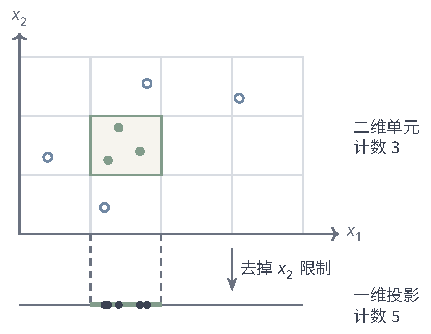
\includegraphics[width=72.912mm]{figures/04-classic-models/00-shared/tikz/clustering-subspace/figure.pdf}
  \caption{CLIQUE 的投影计数示意。二维高亮单元含三个样本，其在横轴区间上的投影还包含其他纵坐标范围的样本。取共同阈值 $\tau=3$，二维单元密集必然推出对应一维单元密集，反方向则不成立。}
 \label{fig:clustering-subspace}
\end{figure}

\subsubsection{参数学习}

CLIQUE 借鉴 Apriori 的逐层候选生成。扫描数据找到一维密集单元后，把具有兼容低维区间的单元连接成更高维候选；只有所有低一维投影都密集的候选才继续计数验证。重复直到候选为空或达到搜索维数上限。

在保留下来的子空间中，算法连接相邻密集单元，形成簇，并可用轴对齐区域的析取式压缩簇描述。原始方法还包含选择子空间和简化描述的步骤；若使用额外启发式筛选，完整性应相对于筛选后的搜索范围表述。

\subsubsection{理论分析}

\paragraph{表达能力}
CLIQUE允许客户群组只在金额和频次坐标上集中，而对年龄不加限制。它可以表达“在这两个坐标中落入某个区域”的群组，也允许同一客户在年龄子空间属于另一簇。如果目标分组还依赖被省略的年龄，那么两条所选坐标相同、年龄不同的记录在这个候选中就无法区分。子空间选择消除了无关坐标的干扰，也舍弃了这些坐标能够提供的区别。

固定子空间后，候选区域是轴对齐单元的并。网格本身对边界的逼近可以独立核验：设所选子空间有$s$个坐标，输入取值位于$[0,1]^s$，等宽网格边长为$h$，目标是其中一个闭合区域$A$。用所有与$A$相交的单元组成$A_h$，则$A\subseteq A_h$；每个多纳入的位置与$A$边界的距离至多为单元直径$\sqrt s\,h$。因此在所选坐标的分布$P_S$下，表示误差满足
\[
 P_S(A_h\mathbin{\triangle}A)
 \leq P_S\{\operatorname{dist}(\bm X_S,\partial A)
                 \leq\sqrt s\,h\}.
\]
当边界上的概率质量为零，右侧随$h\to0$趋零，说明网格可以逐步逼近该区域。CLIQUE实际只保留达到计数阈值的单元，未必恰好选到这些相交单元；细网格还会让质量分散，造成计数不足。这个几何界因而说明候选能表达多少边界细节，并未保证算法恢复$A$。

倾斜关系还会改变所需单元数。例如，二维样本沿$y=x$分布时，两个单坐标都有较大跨度，但方向$(1,-1)$上的变化可以很小。坐标子集没有这个方向；CLIQUE只能用一串较细单元覆盖斜带，再依靠连接组成簇。若要求用一个紧凑的低维方向描述群组，就需要改变候选投影，而不只是调整计数阈值。

\paragraph{收敛性}
CLIQUE 每轮增加候选的维数，最多搜索到 $d$ 维，因此在有限网格上必然结束。除了终止性，还需证明提前剪枝不会遗漏满足计数条件的高维单元；下面的向下封闭性给出这一保证。

\begin{lemma}[子空间密集性的向下封闭性]
 \label{thm:clustering-clique}
 在一致的逐维网格和共同计数阈值 $\tau$ 下，若 $S$ 上的单元 $U$ 密集，则对任意非空 $S'\subseteq S$，其投影 $U|_{S'}$ 也密集。
\end{lemma}
\begin{proof}
记 $I(U)=\{i:\bm{x}_{i,S}\in U\}$。若 $i\in I(U)$，它在 $S$ 的所有选定坐标上都满足区间限制，去掉部分坐标限制后仍然满足。因此
\[
 I(U)\subseteq I(U|_{S'}),\qquad
 n(U|_{S'})\geq n(U)\geq\tau.
\]
投影网格沿用相同区间，故 $U|_{S'}$ 是合法低维单元，并达到同一密集阈值。
\end{proof}

向下封闭性允许根据不密集的低维投影排除高维候选。多个投影各自密集时，其中的样本可能不同，所以高维计数仍需验证。该论证使用共同计数阈值；改为按体积归一的密度或随维数变化的阈值时，需重新核对剪枝条件。

有限网格保证搜索最终结束，但最坏情况下大量投影都密集，仍可能枚举指数多个子空间和单元。

\paragraph{泛化性}
CLIQUE的经验计数可以直接与总体单元质量比较。

\begin{lemma}[固定网格单元的总体质量保证]
 \label{thm:clustering-clique-mass-risk}
设样本独立同分布于$[0,1]^d$，每个坐标预先分成$\xi\geq1$个区间，所有非空坐标子集上的单元组成固定集合$\mathcal U$，其大小为
$N=(1+\xi)^d-1$。记$P_n(U)=n(U)/n$，将计数阈值写成$n t$。对任意$0<\delta<1$，Hoeffding界与并集界给出
\begin{equation}
 P_{D_n}\!\left\{
  \max_{U\in\mathcal U}|P_n(U)-P(U)|
  \leq\alpha_n
 \right\}\geq1-\delta,
 \qquad
 \alpha_n=\sqrt{\frac{\log(2N/\delta)}{2n}}.
 \label{eq:clustering-clique-mass-risk}
\end{equation}
\end{lemma}

因此每个被选中的单元都有$P(U)\geq t-\alpha_n$，每个$P(U)\geq t+\alpha_n$的单元都会被选中。这一结论同时覆盖算法检查过与尚未检查的候选，允许向下封闭剪枝在数据上选择输出。

\begin{theorem}[CLIQUE在固定网格与质量间隔下的期望判定风险界]
 \label{thm:clustering-clique-cell-risk}
若全部单元满足$|P(U)-t|\geq\gamma>0$，且
$n>\log(2N/\delta)/(2\gamma^2)$，经验与总体的密集单元集合以至少$1-\delta$的概率完全相同。固定邻接规则后，它们的连通区域也相同。将风险定义为均匀抽取一个候选单元时，经验密集判定与总体判定不一致的概率，便有
$\mathbb E_{D_n}R_{\mathrm{cell}}\leq\delta$。
\end{theorem}

这里总体目标仍是该网格及阈值定义的区域，并未保证它们对应语义类别。

阈值附近没有间隔时，式\eqref{eq:clustering-clique-mass-risk}只控制区域质量，不能排除一个临界单元改变整体连接。平移网格或自适应选择区间也改变候选集；MAFIA等方法需把这些选择计入复杂度，不能沿用预先固定网格的$N$。

\subsubsection{优化表达能力}

\paragraph{支持子空间中的非凸群组}
固定网格可能把一条密集点带切散到多个未达阈值的单元中。Kailing、Kriegel与Kr\"oger在2004年的SUBCLU中改用子空间内的DBSCAN密度连通，保留坐标子集搜索，同时让邻域连接承担区域构造\scite{clust-kailing2004}。它能在所选坐标中保留弯曲密集路径，不再要求路径逐格达到统一计数。代价是各候选子空间都需要密度查询；核心桥接与密度尺度冲突也仍然存在。

\paragraph{支持倾斜方向的群组关系}
坐标子集无法直接保留变量之间的倾斜关系。ORCLUS进一步学习任意方向的低维正交投影，把相关方向纳入候选，同时增加方向估计和矩阵计算\scite{clust-aggarwal2000}。

沿$y=x$的斜带说明二者的差别。假设$\bm X=(T,T)+\bm\eta$，$\mathbb E T=0$、$\operatorname{Var}(T)=v$，噪声$\bm\eta$独立、均值为零且协方差为$\sigma^2\bm I$。任取一个原坐标，其方差都是$v+\sigma^2$；投影到单位方向$(1,-1)/\sqrt2$，方差则只有$\sigma^2$。允许该方向的ORCLUS候选能表达由相关关系形成的低方差群组，只有坐标选择的候选无法得到同样的一维紧凑性。这个改进针对线性方向；若群组沿弯曲流形变化，一个固定线性投影仍可能把不应靠近的部分重叠，不能据此推得任意非线性结构都可恢复。

\subsubsection{优化计算能力}

\paragraph{适应各坐标的聚集尺度}
各坐标上的聚集尺度不同时，统一区间宽度可能浪费搜索，也可能把局部群体切散。Nagesh、Goil与Choudhary在2001年的MAFIA中采用自适应网格，使候选区间随数据分布调整\scite{clust-nagesh2001}。这种调整减少无效网格与候选检查，同时增加区间估计及合并的成本。区域仍由坐标区间组成，自适应宽度没有增加任意方向的投影。

\paragraph{降低紧凑子空间群组的搜索成本}
若目标是在相关坐标中寻找紧凑群体，还可以用抽样减少完整候选枚举。Procopiuc等在2002年提出DOC与FASTDOC，用随机抽样寻找包含足够多对象的投影盒子\scite{clust-procopiuc2002}。它们另行规定盒宽与群组评价，因而不是对CLIQUE搜索作等价加速。超出给定宽度的细长路径不会成为同一个紧凑候选，增大宽度又可能纳入邻近群体；抽样预算则决定哪些候选会被检查。

\subsubsection{支持子空间簇唯一归属场景}

CLIQUE允许同一对象在不同子空间获得重叠解释。若任务要求每个对象只进入一组，就需要在群组之间协调归属。\term{投影聚类}（projected clustering）通常采用硬划分，并为每簇寻找相关子空间。PROCLUS使用类似K-medoids的代表搜索，在分配与相关坐标选择之间迭代；每簇的坐标可以不同，输出却要求对象有唯一归属\scite{clust-aggarwal1999}。这会放弃一部分重叠解释，同时减少后续使用多份分组的歧义。

\subsubsection{小结}

CLIQUE适合寻找只在部分坐标上集中的群组，允许同一对象获得多个子空间解释。逐层计数筛选减少候选检查，网格与阈值则共同决定边界细节和计数是否足够。

网格边界、区间尺度与搜索规模带来不同限制。SUBCLU用密度连接减少固定网格边界的影响，MAFIA调整区间以适应局部尺度，DOC用抽样寻找另一种紧凑投影目标。若需要唯一归属或倾斜方向，则应比较投影聚类路线。它们分别增加密度查询、自适应网格、抽样或方向估计的代价，不能只根据“支持高维”选择。

\subsection{模型对比与总结}

这一组方法分别处理访问成本和相关变量选择。STING将对象汇入多层网格摘要，使区域查询不必反复访问每条记录；摘要层级较粗时，也会丢失边界细节。CLIQUE则搜索哪些坐标子集存在密集区域，回应全空间距离被无关坐标掩盖的问题，并允许同一对象获得多个子空间解释。两者都使用网格，前者侧重摘要查询，后者侧重发现相关坐标，不能仅凭数据规模决定它们可以互换。

CLIQUE的固定单元又产生边界和尺度限制。SUBCLU保留子空间搜索，用密度连接替代逐格计数，更适合相关坐标中的弯曲路径；MAFIA保留网格表示，用自适应区间回应各坐标聚集尺度不同的问题。DOC与FASTDOC另设紧凑投影盒目标，以抽样减少候选检查。它们分别改变区域构造、区间尺度和搜索对象，节省的工作与可能遗漏的结构也不同。

输出和方向是另一组区别。PROCLUS让每个对象获得唯一归属，并为不同簇选择不同坐标，适合需要一份可直接使用的划分；ORCLUS继续放宽坐标轴限制，用任意线性方向保留倾斜的低方差群组。唯一归属会放弃重叠解释，方向估计则增加参数与计算。应先确定要保留坐标关联、倾斜关系还是多份群组解释，再检查网格、距离和搜索预算。

\section{基于层次的聚类}
\label{sec:clustering-hierarchy}

探索阶段的群组粒度尚不明确时，可以保留多个层级。\term{层次聚类}（hierarchical clustering）用\term{树状图}（dendrogram）记录嵌套的合并或分裂，使分析者从同一棵树读取不同规模的划分。具体截取哪一层，仍由任务用途与证据确定。

凝聚方法从单点向上合并，分裂方法从全集向下拆分。图~\ref{fig:clustering-dendrogram}在同一棵树上读取两种粒度；截线保留已完成的层次决策，不对该粒度重新搜索。

\begin{figure}[htbp]
  \centering
  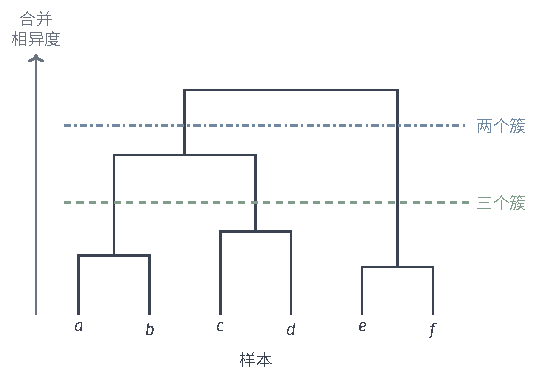
\includegraphics[width=90.914mm]{figures/04-classic-models/00-shared/tikz/clustering-dendrogram/figure.pdf}
  \caption{教学用层次树。叶节点为六个样本，内部节点高度表示合并相异度。较低截线得到三个簇，较高截线得到两个簇；图中高度为示意数值。}
 \label{fig:clustering-dendrogram}
\end{figure}

\subsection{AGNES（凝聚层次聚类）}
\label{sec:clustering-agnes}

若希望先找出最相近的客户，再观察这些小群体怎样组成较大群体，可以从每个样本各自成簇开始。\term{凝聚分析}（Agglomerative Nesting, AGNES）每次合并当前相异度最小的两簇，把合并次序与相异度保存在树中。我们可以在不同高度截取划分，无须预先固定一个$K$；已经合并的对象则不会在后续分开。Kaufman与Rousseeuw在1990年的专著中将这一长期用于数值分类学的过程与自顶向下的DIANA并列介绍。簇内出现多个样本之后，怎样定义簇间相异度就成为下一步的关键。

链接准则把不同群组偏好写进合并决策：单链接沿最近联系扩展，平均链接综合跨簇距离，Ward在1963年以最小SSE增量选择合并。凝聚方向规定构造顺序，链接准则决定哪种关系先进入树。

\subsubsection{模型结构}

初始划分为 $\mathcal{P}^{(0)}=\{\{1\},\ldots,\{n\}\}$。第 $t$ 步选择使 $D(A,B)$ 最小的两个当前簇，替换为 $A\cup B$，经过 $n-1$ 次合并得到根节点。固定相异度和确定的平局规则后，整棵树随之确定。

不同\term{链接方式}（linkage）用不同的簇间统计量：
\begin{align*}
 D_{\mathrm{single}}(A,B)
   &=\min_{i\in A,j\in B}\delta(\bm{x}_i,\bm{x}_j),\\
 D_{\mathrm{complete}}(A,B)
   &=\max_{i\in A,j\in B}\delta(\bm{x}_i,\bm{x}_j),\\
 D_{\mathrm{average}}(A,B)
   &=\frac{\sum_{i\in A,j\in B}\delta(\bm{x}_i,\bm{x}_j)}
   {|A||B|}.
\end{align*}
单链接沿近邻链扩展，可以保留细长形状，也容易被稀疏桥接点连接起来；全链接控制跨簇最远距离，倾向紧凑群组；平均链接考虑所有跨簇样本对，减弱单个极值的影响。这里的平均链接指按样本数加权的 UPGMA。

若样本处于欧氏空间，Ward 链接以合并引起的 SSE 增量定义相异度：
\[
 D_{\mathrm{Ward}}(A,B)
 =\mathrm{SSE}(A\cup B)-\mathrm{SSE}(A)-\mathrm{SSE}(B).
\]
它与 K-means 共享平方误差准则，但只允许合并已有簇。Ward 的原始工作明确以这种误差增量组织层次\scite{ward1963}。

\subsubsection{参数学习}

实现 AGNES 时，可以维护当前簇间的相异度，并在每次合并后更新相关行列。算法~\ref{alg:clustering-agnes} 省去了不影响定义的矩阵下标管理。

\begin{algorithm}[凝聚层次聚类]
 \label{alg:clustering-agnes}
 \begin{algorithmic}[1]
 \Require 样本相异度、链接方式和确定的平局规则
 \Ensure 包含合并高度的层次树
 \State 建立 $n$ 个单点簇，初始化簇间相异度
 \While{当前簇数大于 $1$}
  \State 选择使 $D(A,B)$ 最小的当前簇对
  \State 记录子簇 $A,B$ 和合并高度 $D(A,B)$
  \State 用 $A\cup B$ 替换 $A,B$
  \State 更新新簇与其他当前簇的相异度
 \EndWhile
 \end{algorithmic}
\end{algorithm}

Lance--Williams 递推使多种链接共享更新形式\scite{clust-lance1967}。
\begin{equation}
 \begin{aligned}
 D(A\cup B,C)={}&\alpha_A D(A,C)+\alpha_B D(B,C)\\
 &+\beta D(A,B)
 +\gamma|D(A,C)-D(B,C)|.
 \end{aligned}
 \label{eq:clustering-lance-williams}
\end{equation}
单链接的系数为 $(1/2,1/2,0,-1/2)$，全链接为 $(1/2,1/2,0,1/2)$，平均链接为 $(|A|/(|A|+|B|),|B|/(|A|+|B|),0,0)$。若 $D$ 直接表示 Ward 的 SSE 增量，令 $s=|A|+|B|+|C|$，则
\[
 \alpha_A=\frac{|A|+|C|}{s},\quad
 \alpha_B=\frac{|B|+|C|}{s},\quad
 \beta=-\frac{|C|}{s},\quad \gamma=0.
\]
软件也可能存储Ward增量的缩放平方根；递推系数应与其距离约定配套。

朴素实现每轮扫描全部簇对，约需$O(n^3)$时间和$O(n^2)$存储。链接结构可减少搜索：SLINK的单链接为$O(n^2)$时间和$O(n)$辅助空间，CLINK提供全链接的紧凑表示；平均、全链接和Ward的最近邻链实现也可达到$O(n^2)$时间，常见实现仍保存平方规模距离矩阵\scite{clust-muellner2011}。采用这些算法时需沿用其链接和平局约定。

\subsubsection{理论分析}

\paragraph{表达能力}
层次树能表达细群组逐步包含于粗群组的目标。它的限制也可以用四条记录说明：划分$\{\{a,b\},\{c,d\}\}$与$\{\{a,c\},\{b,d\}\}$不能同时出现在一棵树中，因为两个节点的叶集合只能互不相交或相互包含，而$\{a,b\}$与$\{a,c\}$两者都不满足。若客户按地区和按购买偏好形成交叉群组，一棵嵌套树不能同时完整保留两套关系，需要选择其中一种组织方式或改用重叠输出。

同一粒度下能否表达目标，还取决于链接准则。单链接在高度$h$截取时，得到的是距离不超过$h$的邻接图连通分量；目标若满足簇内有这样的路径、簇间没有这样的边，就会被准确保留，形状可以非凸。加入一串间距不超过$h$的桥接点，又会迫使两端合并。全链接在高度$h$形成的每簇直径不超过$h$，因为每次合并要求所有跨簇距离不超过$h$；因此不能将直径大于$h$的完整环形目标保留为一簇。平均链接综合跨簇距离，不提供同样的直径约束。Ward限定每次合并的平方失真增量，并非逐粒度重新求最小SSE。

\paragraph{收敛性}
AGNES每次合并使簇数减一，因而有限终止。要解释优化性质，还需确定链接所比较的目标；下面证明Ward对当前下一次合并的最优性。

\begin{lemma}[Ward 合并的贪心最优性]
 \label{thm:clustering-ward}
 对欧氏样本的任一当前划分，Ward 链接选择使下一步总 SSE 增量最小的簇对；任意两个非空簇满足
 \[
 \Delta\mathrm{SSE}(A,B)
 =\frac{|A||B|}{|A|+|B|}
   \lVert\bm{\mu}_A-\bm{\mu}_B\rVert_2^2.
 \]
\end{lemma}
\begin{proof}
令 $a=|A|$、$b=|B|$，则合并均值为 $\bm{\mu}=(a\bm{\mu}_A+b\bm{\mu}_B)/(a+b)$。由式~\eqref{eq:clustering-mean-decomposition}，合并后的 SSE 等于两簇原有 SSE 加上
\[
 a\lVert\bm{\mu}_A-\bm{\mu}\rVert_2^2+
 b\lVert\bm{\mu}_B-\bm{\mu}\rVert_2^2.
\]
又有 $\bm{\mu}_A-\bm{\mu}=b(\bm{\mu}_A-\bm{\mu}_B)/(a+b)$，另一项为其相反方向的 $a/b$ 倍。代入后系数为 $(ab^2+ba^2)/(a+b)^2=ab/(a+b)$。其他簇不变，因此选择最小 Ward 相异度恰好最小化当前总 SSE 增量。
\end{proof}

Ward的最优性范围是当前可合并的簇对。截取$K$簇后，若再允许样本重新分配，可继续用K-means降低SSE；此时搜索范围已从合并已有簇扩展为逐点分配，因此结果可以不同。

单链接可由完整加权图的最小生成树解释：按边权递增连接，得到同一阈值连通结构，等权边可对应不同二叉表示。全链接比较跨簇最大距离，Ward比较总平方误差增量；各准则优化当前合并，整棵树由这些局部选择累积形成。

\paragraph{泛化性}
AGNES与DIANA输出当前对象的层次树，树上没有预先定义的独立新点损失。重采样中重复出现的分支可以作为稳定性证据，仍不能替代期望风险界；相异度接近的早期合并尤其可能改变后续树形。

若用途是将新点分配给某一截取层，可以明确规定一个可检验的扩展：保留$K$个簇的均值，冻结它们，并对新点按最近均值分配。对$\lVert\bm X\rVert_2\leq r$的独立同分布欧氏样本，这一学习器的量化风险满足式\eqref{eq:clustering-kmeans-risk}，其中$e_n$是所保留中心的经验最近中心损失与全局最优量化损失之差。树的原成员未必等于最近中心分配，所以该式评价冻结中心的预测规则，不能直接评价树上每个分支。Ward的贪心合并、二分K-means及BIRCH后的中心压缩都可能影响$e_n$，并未改变经验偏差项。

\subsubsection{优化表达能力}

\paragraph{保留非球形群组的边缘结构}
用单个中心合并两个弯曲或拉长的群组，可能漏掉它们实际相邻的边缘；只用最近样本，又可能被一两个孤立点连接起来。CURE在两者之间取折中，用多个分散代表点覆盖每簇的不同部分，再把这些点向均值收缩，以减弱极端位置的影响\scite{clust-guha1998}。选择代表时，先选离均值较远的点，再逐个选择离已有代表集合较远的点。若原代表为$\bm{r}$、簇均值为$\bm{\mu}_C$，收缩后的代表可写为
\[
 \bm{r}'=(1-\alpha)\bm{r}+\alpha\bm{\mu}_C,
 \qquad 0\leq\alpha\leq1.
\]
两个簇的代表之间的最近距离用于决定合并。$\alpha=0$ 保留边缘形状，也更易受极端点影响；$\alpha$ 接近 1 时，代表逐渐退化为中心。CURE用抽样和分区减少参与完整层次搜索的对象，成本需同时计入抽样分配、代表更新及实际合并规模。

CURE增加了描述簇边缘的位置，因而可以在代表覆盖充分时比较细长或弯曲群组的局部间隔。它仍只能看见所选代表，未被代表覆盖的细小分支可能不参与合并判断。收缩也会改变目标间隔：若两圈的均值都为圆心，$\alpha=1$时所有代表都退到同一点，原本分离的两个环便无法靠代表距离区分。多个代表缓解单中心限制，代表数和收缩量则决定保留了多少形状信息。

\paragraph{适应不同群组的内部连接尺度}
群组内部的疏密不同，还会使统一的绝对距离阈值难以决定合并：对一个稠密簇很远的间隔，对稀疏簇可能只是通常的间隔。Chameleon先在近邻图上形成子簇，再把簇间连接和距离与各簇内部的对应量比较，按相对互连度与相对相近度合并\scite{clust-karypis1999}。它让合并判断随群组内部结构调整，已完成合并仍限制后续层次。

这让簇内通常间隔较大的稀疏区域不必与稠密区域使用同一个绝对合并尺度。收益成立的前提是初始子簇与近邻图保留了这些内部结构；被初始划分切断的连接或错误加入的跨群组强边，会改变随后比较的相对量。合并阶段只能组合已有子簇，若一个子簇已经混入两个目标群组，就不能再将它们分开。

\paragraph{利用类别属性的共同邻居}
对于类别属性，两条客户记录可能只共享少量属性，却与同一批其他记录相似。ROCK把这种共同支持纳入合并依据，用共同邻居形成的链接数量替代单纯点间距离，其工作发表于1999年\scite{clust-guha1999}。共享邻居能补充直接相似度，但邻居怎样定义仍决定哪些支持会被计入，也带来额外统计成本。

例如，两条记录没有直接邻接，但各自的邻居集合有三个共同对象，链接计数就保留了这份间接关系；若共同邻居为空，单凭这一对的链接则不能区分“同群体的两条孤立记录”与“不相关记录”。ROCK所能利用的目标结构必须反映在邻居重叠中。共享一个高连接对象还可能给不同群组增加共同支持，不能把共同邻居多直接解释为语义同类。

\subsubsection{优化计算能力}

层次搜索若直接保存全部对象及大量点对距离，数据装不进内存时就难以执行。Zhang、Ramakrishnan与Livny在1996年的BIRCH中先把邻近对象汇为可合并的摘要，再对摘要作聚类。它主要减少进入后续搜索的对象数，可以搭配相应的凝聚过程，而不是改变所有层次方法的目标。它用\term{聚类特征}（clustering feature, CF）记录样本数、向量和与平方范数和\scite{clust-zhang1996}。这些摘要写为
\[
 \mathrm{CF}(C)=
 \left(|C|,\ \sum_{i\in C}\bm{x}_i,\
 \sum_{i\in C}\lVert\bm{x}_i\rVert_2^2\right).
\]
这些量可相加，也可恢复均值和簇内平方误差。CF树将邻近样本汇入摘要，再对叶摘要聚类。树高和摘要规模受控时，扫描成本近似随$n$线性增长；摘要阈值、插入顺序及压缩损失共同影响最终划分。

CF对均值与SSE是充分的摘要，却不是对簇形状的完整表示。以一维教学例说明：$\{-1,-1,1,1\}$与$\{-\sqrt2,0,0,\sqrt2\}$都得到$\mathrm{CF}=(4,0,4)$，前者集中在两个位置，后者集中在三个位置。若各自被压成一个叶摘要，后续只读取CF就无法区分这两种结构，更不能根据其中的间隔重新拆出目标群组。保留更多叶摘要可以增加空间细节，同时增加内存和后续搜索。

\subsubsection{小结}

AGNES逐次合并已有群组，适合希望保留从细到粗嵌套关系的探索。链接准则决定一次合并看哪种关系：单链接关注局部连接，全链接限制最远跨度，Ward关注平方重构代价。不可撤销的合并使早期误合并传到后续层级，换一个链接并不能消除这项限制。

数据规模与簇形状可以分别处理。BIRCH先压缩对象，减少完整层次搜索的规模；CURE用多个收缩代表保留更多边缘位置；ROCK与Chameleon则改变合并所依据的关系。摘要可能损失细节，代表需要更新，关系图需要构造，这些代价应与当前距离存储和合并预算一起比较。

\subsection{DIANA（分裂层次聚类）}

有时我们更关心“整个数据先分成哪几大部分”，而非最先配对的几个样本。\term{分裂分析}（Divisive Analysis, DIANA）从所有样本组成的一簇开始，优先拆分内部差异最大的群组，再继续细分。与AGNES从局部相近关系向上合并相比，DIANA从整体差异向下建立层次；它采用的贪心拆分并不等于反向执行AGNES，早期分开的样本也不会在后续重新合并。

\subsubsection{模型结构}

DIANA 通常用簇直径 $\max_{i,j\in C}\delta(\bm{x}_i,\bm{x}_j)$ 选择待分裂簇。每次把一个非单点簇拆成两个非空子簇；若展开完整树，恰需 $n-1$ 次分裂。若只需少数大簇，也可提前停止。

\subsubsection{参数学习}

对含 $m$ 个样本的簇，非平凡无序二分共有 $2^{m-1}-1$ 种，完整枚举很快变得昂贵。DIANA 用\term{分裂群}（splinter group）贪心构造二分：选取对其余样本平均相异度最大的样本作为种子，令其自成集合 $S$，其余样本组成 $R$。

对每个 $i\in R$，在 $|R|>1$ 时计算
\[
 a_i=\frac{1}{|R|-1}\sum_{\substack{j\in R\\j\ne i}}
 \delta(\bm{x}_i,\bm{x}_j),\qquad
 b_i=\frac{1}{|S|}\sum_{j\in S}\delta(\bm{x}_i,\bm{x}_j).
\]
若最大的 $a_i-b_i$ 为正，就把对应样本从 $R$ 移到 $S$，再更新这些量；否则结束分裂。这样每一步都选择更接近分裂群的最强候选，而非按任意顺序一次扫描。保留至少一个样本在 $R$ 中，避免产生空子簇。

\subsubsection{理论分析}

\paragraph{表达能力}
DIANA的候选也服从同一嵌套限制，改变构造方向并不会让交叉分组同时进入一棵树。若目标的一个群组被第一次分裂分在两边，继续细分便不能将它重组。反过来，目标若按内部差异逐级细化，树可以保留相应层级；具体分裂群规则能否找到这些层级，还取决于相异度和贪心选择，并非由二分候选数量足够多就能保证。



\paragraph{收敛性}
每次分裂保留两个非空子簇，所以完整树恰有$n-1$次分裂。大小为$m$的待分裂簇中，分裂群已有一个种子，每次只把一个对象移入且不移回，最多再移动$m-2$个对象。两层循环因此都有限。有限二分候选中存在最优者，但分裂群启发式不枚举它们，也没有对某个全树最优目标的收敛保证。

\paragraph{泛化性}
若要评价新点，可在预定的$K$簇层截取树，保留各簇均值，并冻结最近均值预测规则。对独立同分布且范数不超过$r$的欧氏输入，其期望量化风险满足式\eqref{eq:clustering-kmeans-risk}；$e_n$是这些均值的经验最近中心损失与全局最优量化损失之差。这个结论随$n$控制抽样误差，同时保留贪心拆分造成的差距。它评价的是截取后增加的新点规则，并未把整棵层次树的分支稳定性改写为风险保证。

\subsubsection{小结}

DIANA以分裂群启发式减少二分穷举，优先提供顶层结构。相异度、种子和平局影响分裂，距离缓存、簇规模与更新方式影响成本。比较AGNES时，应在相同数据与稳定性协议下检查关键群组，而非仅凭搜索方向推断哪种更稳。

\subsection{模型对比与总结}

AGNES与DIANA都保留嵌套群组，区别在怎样构造这棵树。AGNES从单个对象逐步合并，链接准则决定先保留近邻连接、紧凑团块还是平方误差较小的合并；DIANA从全体对象逐步分裂，用分裂群启发式避免枚举所有二分，先提供顶层区别。改变方向并没有允许后续撤销已完成的分支：希望保留的群组一旦被早期操作分开或混合，后续粒度选择就会受限。

大样本和复杂形状要求在凝聚前后做不同调整。BIRCH先压缩邻近对象，使后续搜索处理较少摘要；CURE用多个收缩代表补充单中心遗漏的簇边缘。前者优先减少对象访问，后者优先保留形状，摘要阈值、代表数和收缩量也分别控制信息损失。它们可以降低大样本搜索成本，仍需检查稀少群体和细小分支有没有进入摘要或代表。

关系与尺度差异则改变合并依据。ROCK用共同邻居补充类别对象的间接相似关系；Chameleon把跨簇联系与簇内结构比较，避免稠密和稀疏区域共用一个绝对合并尺度。它们都需要可靠的初始关系，图中错误连接可能被后续合并放大。这些路线是在不同环节调整层次构造，并非一串按年份替代前人的方法。

若任务还要求估计对象来自某个生成成分的概率，层次树本身没有规定这一概率，需要进一步建立与数据相符的生成模型。

\section{基于概率的聚类}
\label{sec:clustering-probabilistic}

中心、密度连通与图割规定了群组结构。若任务还要求估计新样本来自某种群体的概率，可以假设样本先选择潜在成分，再由该成分分布生成。概率聚类据此共同估计分布参数和成分归属后验。

生成模型支持软归属、预测密度与模型比较。其成分含义需与任务群组核对：一个复杂形状的群体可能需要多个高斯近似，因此拟合密度所需的成分数与语义类别数可以不同。

\subsection{高斯混合模型（GMM）}
\label{sec:clustering-gmm}

考虑两个椭圆状的客户群组：一组沿消费金额方向伸展，另一组沿购买频次方向伸展。离两个中心同样远的记录，在前一组的主要变化方向上可能很常见，在后一组的窄方向上却很罕见。只比较中心的欧氏距离没有表达这种区别。\term{高斯混合模型}（Gaussian Mixture Model, GMM）为每个成分设置均值、协方差与权重，用它们共同计算样本的密度及成分归属概率。协方差描述各方向的伸展程度，权重描述成分在总体中的比例；重叠区域内的样本可以同时对多个成分有非零后验概率。现代教材常结合EM说明其估计\scite{bishop2006}。

Pearson 在 1894 年的研究中，用两个正态分布的混合拟合一组生物测量数据，并通过矩方程估计参数\scite{clust-pearson1894}。关键想法是：观测到的一个总体，可能混合了多个未被直接标注的子总体。分布中的多个成分因此可以作为隐含群组的统计表示。

Wolfe在1970年将多元混合分析用于模式聚类，连接多维成分表示与似然估计\scite{clust-wolfe1970}。Dempster、Laird与Rubin在1977年提出一般EM框架，处理潜变量未观测时的参数更新。GMM规定生成分布，EM规定如何估计，两者可以分别改变。

GMM同时使用均值、协方差和成分权重。协方差决定偏离均值的方向尺度，权重决定成分的相对比例；样本归属由这些量的共同密度贡献确定，软后验因此包含比中心距离更多的信息。

\subsubsection{模型结构}

与第\ref{sec:classification-gda}节的 GDA 相比，两者都用高斯密度描述输入，但 GDA 的类别标签已经观测，可以按类直接估计；GMM 的成分归属不可观测，需要作为潜在成分变量推断。具体而言，先按权重 $\pi_k\geq0$、$\sum_k\pi_k=1$ 抽取潜在成分变量 $z_i\in\{1,\ldots,K\}$，再从 $\mathcal{N}(\bm{\mu}_{z_i},\bm{\Sigma}_{z_i})$ 抽取样本。要求 $\bm{\Sigma}_k\succ0$，边际密度为
\begin{equation}
 p(\bm{x};\bm{\theta})
 =\sum_{k=1}^K\pi_k
   \mathcal{N}(\bm{x};\bm{\mu}_k,\bm{\Sigma}_k),
 \label{eq:clustering-gmm}
\end{equation}
其中 $\bm{\theta}$ 汇集权重、均值与协方差。独立同分布样本的对数似然为
\[
 \ell(\bm{\theta})
 =\sum_{i=1}^n\log\left[
 \sum_{k=1}^K\pi_k
 \mathcal{N}(\bm{x}_i;\bm{\mu}_k,\bm{\Sigma}_k)\right].
\]
求和藏在对数内，使每个成分的参数无法独立优化。

给定参数后，贝叶斯公式给出\term{责任度}（responsibility），即当前模型认为样本由某成分产生的后验概率：
\begin{equation}
 \gamma_{i,k}
 =\frac{\pi_k\mathcal{N}(\bm{x}_i;\bm{\mu}_k,\bm{\Sigma}_k)}
 {\sum_{j=1}^K\pi_j
       \mathcal{N}(\bm{x}_i;\bm{\mu}_j,\bm{\Sigma}_j)}.
 \label{eq:clustering-responsibility}
\end{equation}
责任度每行和为1，可作为软归属；硬划分取$\argmax_k\gamma_{i,k}$并处理平局。概率含义对应当前生成模型中的成分，解释为任务类别还需核对模型与语义的关系。

图~\ref{fig:clustering-gmm-responsibilities}固定两成分模型。上图相加各加权密度，得到观测总密度；下图把各成分贡献除以总密度，得到$\gamma_k(x)=p(z=k\mid x;\bm{\theta})$。对称点$x=0$的责任度各为一半，其他位置连续变化。成分归属与总密度的峰数描述不同结构，两成分混合也可能只有一个峰。

\begin{figure}[tbp]
  \centering
  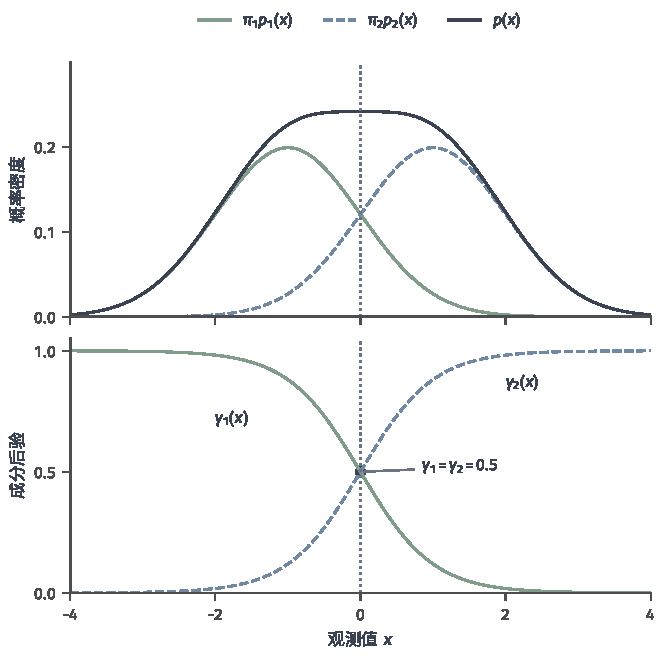
\includegraphics[width=105.412mm]{figures/04-classic-models/00-shared/matplotlib/clustering-gmm-responsibilities/figure.pdf}
  \caption{两成分 GMM 的密度与软归属。设 $\pi_1=\pi_2=1/2$、$\mu_1=-1$、$\mu_2=1$，两个方差均为 1，$p_k(x)$ 表示第 $k$ 个高斯密度。上图展示加权成分密度及其和，下图展示同一观测值对应的后验；颜色与线型在两图中保持一致。}
 \label{fig:clustering-gmm-responsibilities}
\end{figure}

\subsubsection{参数学习}

\term{期望最大化}（Expectation-Maximization, EM）交替估计潜在成分变量的分布和优化参数，Dempster、Laird 与 Rubin 将这一原则统一为一般框架\scite{clust-dempster1977}。E 步用当前参数 $\bm{\theta}^{(t)}$ 计算式~\eqref{eq:clustering-responsibility}；M 步固定这些责任度，最大化完全数据对数似然的期望。潜在成分变量不再藏在对数的求和中，而是通过 E 步给出的分布参与加权。

忽略与参数无关的常数，M 步目标为
\begin{equation}
 \begin{aligned}
 Q(\bm{\theta}\mid\bm{\theta}^{(t)})
 =\sum_{i,k}\gamma_{i,k}^{(t)}
 \biggl[&\log\pi_k-\frac12\log\det\bm{\Sigma}_k\\
 &-\frac12(\bm{x}_i-\bm{\mu}_k)^\top
 \bm{\Sigma}_k^{-1}(\bm{x}_i-\bm{\mu}_k)\biggr].
 \end{aligned}
 \label{eq:clustering-gmm-q}
\end{equation}
M步把责任度看作固定的样本权重，分别重新估计成分比例、均值和协方差。记有效样本量$n_k^{(t)}=\sum_i\gamma_{i,k}^{(t)}$。对于成分比例，在$\sum_k\pi_k=1$的约束下最大化$\sum_k n_k^{(t)}\log\pi_k$；加入拉格朗日乘子后，驻点满足$n_k^{(t)}/\pi_k=\lambda$，再对$k$求和得到$\lambda=n$。对于均值，$Q$中的相关项是责任度加权的负平方Mahalanobis距离。令其对$\bm\mu_k$的梯度为零，消去公共的正定因子$\bm\Sigma_k^{-1}$，就得到加权残差和为零。因此，这两项更新分别为
\begin{equation}
 \pi_k^{(t+1)}=\frac{n_k^{(t)}}{n},\qquad
 \bm{\mu}_k^{(t+1)}
 =\frac{\sum_i\gamma_{i,k}^{(t)}\bm{x}_i}{n_k^{(t)}}.
 \label{eq:clustering-gmm-mean}
\end{equation}
每个样本按其责任度贡献一部分计数与观测值，硬分配中的簇规模和簇均值由此变为有效样本量与加权均值。

再令精度矩阵 $\bm{\Lambda}_k=\bm{\Sigma}_k^{-1}$，加权散布为
\[
 \bm{S}_k=\sum_i\gamma_{i,k}^{(t)}
 (\bm{x}_i-\bm{\mu}_k^{(t+1)})
 (\bm{x}_i-\bm{\mu}_k^{(t+1)})^\top.
\]
把协方差改写为精度矩阵后，$Q$中需要最大化的部分为$\tfrac12[n_k^{(t)}\log\det\bm{\Lambda}_k-\operatorname{tr}(\bm{\Lambda}_k\bm{S}_k)]$。令这一部分的矩阵梯度为零，得到$n_k^{(t)}\bm{\Lambda}_k^{-1}-\bm{S}_k=\bm{0}$；换回协方差，就得到加权散布除以有效样本量：
\begin{equation}
 \bm{\Sigma}_k^{(t+1)}
 =\frac{\bm{S}_k}{n_k^{(t)}}.
 \label{eq:clustering-gmm-covariance}
\end{equation}
更新要求有效样本量为正。加权散布正定时，无约束协方差取得正定域内的有限最优；退化散布则需要协方差约束或其他估计。

代码~\ref{code:clustering-gmm}在对数域计算责任度，并用协方差特征值下界$\epsilon$避免塌缩。该截断求解固定约束$\bm{\Sigma}_k\succeq\epsilon\bm{I}$下的M步；每轮任意加常数矩阵则对应另一种估计，需另说明目标。

\begin{codeblock}[language=Python,label={code:clustering-gmm}]{带协方差下界的 GMM--EM}
import numpy as np
from scipy.special import logsumexp
from scipy.stats import multivariate_normal

def gmm_em(X, K, max_iter=100, tol=1e-5, eps=1e-6):
    X = np.asarray(X, dtype=float)
    n, d = X.shape
    if eps <= 0:
        raise ValueError("eps must be positive")
    _, mu = kmeans(X, K)
    pi = np.full(K, 1.0 / K)
    cov = np.repeat((max(1., eps) * np.eye(d))[None], K, axis=0)
    def e_step():
        log_p = np.column_stack([
            np.log(pi[k]) + multivariate_normal.logpdf(
                X, mean=mu[k], cov=cov[k])
            for k in range(K)])
        normalizer = logsumexp(log_p, axis=1)
        gamma = np.exp(log_p - normalizer[:, None])
        return gamma, normalizer.sum()
    gamma, ll = e_step()
    for _ in range(max_iter):
        nk = gamma.sum(0)
        if (nk <= 0).any():
            raise ValueError("numerically empty component")
        pi = nk / n
        mu = (gamma.T @ X) / nk[:, None]
        for k in range(K):
            diff = X - mu[k]
            S = (diff * gamma[:, k, None]).T @ diff / nk[k]
            values, vectors = np.linalg.eigh(S)
            cov[k] = (vectors * np.maximum(values, eps)) @ vectors.T
        gamma, new_ll = e_step()
        if abs(new_ll - ll) <= tol * (1 + abs(ll)):
            break
        ll = new_ll
    return pi, mu, cov, gamma
\end{codeblock}

该实现调用前文的 K-means，以其中心初始化，返回的责任度由最终参数重新计算。协方差特征值截断之所以是上述受限 M 步的解，是因为最优协方差与加权散布共享特征向量，每个特征值分别最小化 $\log s+\lambda/s$，在 $s\geq\epsilon$ 上得到 $s=\max\{\lambda,\epsilon\}$。计算中可同时记录似然变化、不同重启的目标和近空成分，以检查数值误差及初始化影响。

完整协方差保留全部二阶方向关系；类内有效样本不足时，可采用对角、球形或共享协方差减少自由度。完整形式一轮约需$O(nKd^2+Kd^3)$运算，立方项来自矩阵分解，对角形式的主要成本为$O(nKd)$。K-means++、重启和初始划分协方差可提供不同起点，其结果在同一约束与似然下比较。

\subsubsection{理论分析}

\paragraph{表达能力}
GMM要逼近的是输入密度，成分后验再由这个密度表示决定。若总体确由$K$个满足候选协方差条件的高斯成分混合生成，真密度就在候选族中，可以达到零KL逼近误差。反过来，一个高斯只能形成一个椭圆状密度峰；每个非退化高斯在全空间为正，有限混合也不能精确表示具有正测度零密度区域的目标，尾部仍不能等同于幂律等重尾分布。增加成分可以改善这些分布的近似，却不等于消除了固定$K$的失配。

协方差限制带来的误差也可以明确计算。假设二维目标是均值为零、协方差为
\[
 \bm\Sigma_\star=
 \begin{pmatrix}1&\rho\\\rho&1\end{pmatrix},
 \qquad 0<|\rho|<1
\]
的高斯分布。一个完整协方差成分可以准确表达它；若只允许一个对角协方差成分，最优均值仍为零、两个最优方差仍为1，但最小KL误差为
\[
 \inf_{\bm\mu,\,\bm\Sigma\text{ 对角}}
 D_{\mathrm{KL}}\bigl(\mathcal N(\bm0,\bm\Sigma_\star)
                 \Vert\mathcal N(\bm\mu,\bm\Sigma)\bigr)
 =-\tfrac12\log(1-\rho^2)>0.
\]
这是将高斯对数密度对目标取期望后，分别最小化均值项和两个方差项得到的结果；遗漏的相关方向由行列式$1-\rho^2$留下误差。多个对角成分可以用不同位置补充这种相关形状，但此时增加的是成分数，不能把单成分限制的结论直接套给整个混合族。

允许成分数增加时，密度逼近可以由一个具体构造说明。设$f$是$\mathbb R^d$上连续且具有紧支撑的概率密度，$\varphi_\sigma$为协方差$\sigma^2\bm I$的零均值高斯密度。把支撑划成直径不超过$\Delta$的有限单元，在每个单元$U_j$内选一个位置$\bm\mu_j$，并令$\pi_j=\int_{U_j}f$。将零质量单元略去，得到合法混合
\[
 p_{\sigma,\Delta}(\bm x)
 =\sum_j\pi_j\varphi_\sigma(\bm x-\bm\mu_j).
\]
先以卷积平滑$f$，再把每个单元中的连续中心移到$\bm\mu_j$，两步误差满足
\[
 \lVert f-p_{\sigma,\Delta}\rVert_{L^1}
 \leq\lVert f-f*\varphi_\sigma\rVert_{L^1}
       +\sqrt{2/\pi}\,\Delta/\sigma.
\]
第二项来自高斯密度沿位移方向的导数积分：两个同协方差高斯的$L^1$距离不超过$\sqrt{2/\pi}$乘以均值距离再除以$\sigma$。第一项随$\sigma\to0$趋零，因为密度平移的$L^1$差趋零，卷积只是在高斯位移下平均这些差。故选择$\sigma\to0$、$\Delta/\sigma\to0$，有限混合就能把这类目标的$L^1$误差降到任意小。这个结论允许成分数增加、方差缩小，不适用于固定$K$或固定正方差下界的候选族，也未给出KL误差或语义簇恢复保证。一个弯曲群体可能需要沿其形状布置多个高斯，因而密度拟合所需的成分数可以大于群体数。

\paragraph{收敛性}
EM在旧参数处构造与观测似然相等的下界，再提高这一辅助目标。这样可避免直接优化对数内的成分求和；精确E步与M步改进条件共同给出似然不下降。

\begin{theorem}[GMM的精确EM迭代的似然上升性质]
 \label{thm:clustering-em}
 E 步取当前精确后验，M 步满足
 $Q(\bm{\theta}^{(t+1)}\mid\bm{\theta}^{(t)})
 \geq Q(\bm{\theta}^{(t)}\mid\bm{\theta}^{(t)})$。
 在相关概率与期望有限、支持条件允许下，则
 $\ell(\bm{\theta}^{(t+1)})\geq\ell(\bm{\theta}^{(t)})$。
\end{theorem}
\begin{proof}
对每个样本，令$q_i$相对于当前参数下成分后验的KL散度有限，直接使用整体对数比形式（参考\BookSectionRef{sec:information-elbo-approximation}{卷2《数学准备：概率、因果与决策》第2章“概率分布”第2.5.2节“表示约束下的分布逼近”}）：
\[
 \begin{aligned}
 \mathcal L_i(q_i,\bm\theta)
 &=\sum_{k:q_i(k)>0}q_i(k)
    \log\frac{p(\bm x_i,z_i=k;\bm\theta)}{q_i(k)},\\
 \log p(\bm x_i;\bm\theta)
 &=\mathcal L_i(q_i,\bm\theta)
   +D_{\mathrm{KL}}\bigl(q_i\Vert p(z_i\mid\bm x_i;\bm\theta)\bigr).
 \end{aligned}
\]
对样本求和，把下界记为$\mathcal L(q,\bm\theta)$。该分解不要求$q_i$覆盖后验的全部支撑；
若改用恢复证据的Jensen等式，则必须另查相反方向的覆盖条件。
E 步令 $q_i^{(t)}$ 等于旧参数的后验，因此 $\mathcal{L}(q^{(t)},\bm{\theta}^{(t)})=\ell(\bm{\theta}^{(t)})$。固定 $q^{(t)}$ 后，下界与 $Q$ 仅相差不含参数的熵项，M 步遂给出
\[
 \begin{aligned}
 \ell(\bm{\theta}^{(t+1)})
 &\geq\mathcal{L}(q^{(t)},\bm{\theta}^{(t+1)})\\
 &\geq\mathcal{L}(q^{(t)},\bm{\theta}^{(t)})
 =\ell(\bm{\theta}^{(t)}).
 \end{aligned}
\]
这就证明了单调性。
\end{proof}

似然有上界时，EM的单调性可进一步给出似然值收敛。参数趋于驻点还需连续性、紧性等正则条件，Wu给出了相应分析\scite{clust-wu1983}。驻点可能是局部极大值或鞍点，优化解释应分别核对值的极限、参数极限和驻点类型。

当 $K\geq2$，且模型中存在一个可塌缩的正权重成分，其余正权重成分仍使其他样本的混合密度保持正值时，无约束 GMM 的似然没有上界。令可塌缩成分的均值等于某个样本，协方差为 $\sigma^2\bm{I}$；当 $\sigma\to0$ 时，该样本处的密度按 $\sigma^{-d}$ 增长，而其他样本仍由其余成分覆盖，因此总对数似然可以无界增加。若 $K=1$ 且样本经验散布矩阵正定，单高斯的最大似然有限；若经验散布矩阵奇异，协方差仍可能在数据未占据的方向趋近边界并导致似然退化。协方差下界、适当先验或惩罚可以阻止这类塌缩，但它们各自改变了优化问题。

潜在成分编号的置换不改变混合密度；当成分彼此不同且权重为正时，一个解通常对应 $K!$ 个等价标号。这与不同拟合质量的局部极值是两类问题。

\paragraph{泛化性}
GMM可以为新观测给出密度，因此以对数损失评价泛化：
$R(\bm\theta)=\mathbb E_P[-\log p_{\bm\theta}(\bm X)]$，
$\widehat R_n=-\ell(\bm\theta)/n$。
无约束似然可以塌缩，下面明确采用有界的候选族，而不把EM的似然上升当作统计保证。

\begin{theorem}[GMM在有界参数与非退化协方差下的期望对数风险界]
 \label{thm:clustering-gmm-risk}
设训练样本独立同分布于$P$，$\lVert\bm X\rVert_2\leq r$几乎处处，固定$K$，并在训练前规定
$\lVert\bm\mu_k\rVert_2\leq A$、$a\bm I\preceq\bm\Sigma_k\preceq b\bm I$，其中$0<a\leq b$；权重属于概率单纯形。用均值、权重及对称协方差的独立坐标组成参数向量，协方差坐标按Frobenius范数计量。令
\[
 \begin{aligned}
 p_0&=K+Kd+Kd(d+1)/2,\\
 B_0&=\sqrt{1+KA^2+Kdb^2},\\
 q_-&=(2\pi b)^{-d/2}e^{-(r+A)^2/(2a)},\\
 q_+&=(2\pi a)^{-d/2},\\
 M_0&=\tfrac d2\log(b/a)+\tfrac{(r+A)^2}{2a},\\
 L_0^2&=K(q_+/q_-)^2+\frac{(r+A)^2}{a^2}\\
 &\quad+\frac14\left(\frac{(r+A)^2}{a^2}+\frac{\sqrt d}{a}\right)^2.
 \end{aligned}
\]
混合密度始终介于$q_-$与$q_+$，所以对数损失的取值区间长度至多为$M_0$。均值及协方差的对数密度导数由责任度加权，权重导数则由$q_+/q_-$控制，合并得到参数Lipschitz常数$L_0$。参数集在$p_0$维半径$B_0$的球内，故其$\epsilon$覆盖数至多为$(1+2B_0/\epsilon)^{p_0}$。

对该受约束族的任意学习器，记$e_n$为经验对数损失距全局最优的差。引理\ref{thm:clustering-cover-risk}取$\epsilon=B_0/n$给出
\begin{equation}
 \begin{aligned}
 \mathbb E_{D_n}R(\widehat{\bm\theta})
 &\leq\inf_{\bm\theta\in\Theta}R(\bm\theta)
       +\frac{4L_0B_0}{n}\\
 &\quad+2M_0\sqrt{\frac{p_0\log(1+2n)+\log2}{2n}}
       +\mathbb E_{D_n}e_n.
 \end{aligned}
 \label{eq:clustering-gmm-risk}
\end{equation}
\end{theorem}

高概率版本同样将$\log2$换成$\log(2/\delta)$。约束阻止密度尖峰无限提高训练似然，并使全体候选的训练与新样本损失能够同时比较；EM的局部求解误差保留在$e_n$中。若$P$有密度且熵有限，$R(\bm\theta)-H(P)=\operatorname{KL}(P\Vert p_{\bm\theta})$，上式也给出距该族最佳密度的KL超额风险界。它允许分布失配，不要求参数或成分标号唯一，也不评价语义簇标签。

成分数与协方差形式改变候选族，需另行选择。完整协方差的自由参数数目为
\[
 m_K=(K-1)+Kd+\frac{Kd(d+1)}2,
\]
常用准则为
\begin{equation}
 \mathrm{BIC}(K)=-2\ell(\hat{\bm\theta}_K)+m_K\log n,
 \qquad
 \mathrm{AIC}(K)=-2\ell(\hat{\bm\theta}_K)+2m_K.
 \label{eq:clustering-bic}
\end{equation}
它们用较小值选择候选，并非式\eqref{eq:clustering-gmm-risk}的替代界。BIC的证据近似依赖渐近条件；有限混合存在零权重边界与奇异参数，混合阶数的一致性需核对专门条件\scite{clust-keribin2000}。将所选成分数解释为语义类别数，还需外部知识。

\subsubsection{与中心量化的联系}

GMM的软归属、权重与协方差共同定义后验，K-means只使用中心平方距离。固定部分参数并取小方差极限，可以明确两种目标和更新的联系。固定均匀权重 $\pi_k=1/K$ 和共享球形协方差 $\bm{\Sigma}_k=\sigma^2\bm{I}$，则
\[
 \gamma_{i,k}=
 \frac{\exp(-\lVert\bm{x}_i-\bm{\mu}_k\rVert_2^2/(2\sigma^2))}
 {\sum_j\exp(-\lVert\bm{x}_i-\bm{\mu}_j\rVert_2^2/(2\sigma^2))}.
\]
若 $\bm{x}_i$ 的最近中心唯一为 $k^\ast$，则对任意 $j\ne k^\ast$，距离平方差为正，相应指数比随 $\sigma^2\to0$ 趋零，故 $\gamma_{i,k^\ast}\to1$。M 步的均值更新因此退化为 Lloyd 更新；平局时责任度可分散在多个最近中心，不能直接得到唯一硬簇分配。

去掉只依赖$\sigma$的常数，目标$-2\sigma^2\ell$趋向$\sum_i\min_k\lVert\bm{x}_i-\bm{\mu}_k\rVert_2^2$，给出平方误差的联系。这一极限固定均匀权重并缩小共享球方差；自由协方差GMM优化更大的分布族。FCM的软隶属度则来自模糊损失，与生成后验采用不同定义。

\subsubsection{优化表达能力}

\paragraph{表示二值与计数分布}
高斯成分规定了连续的椭圆分布。二值与计数数据需要先改变观测机制，例如采用伯努利或多项式成分，再按相应似然计算责任度和更新参数。混合结构可以保留，单个成分所描述的关系则随分布而变。

一个按坐标独立的伯努利成分无法表达成分内部任意的二值相关性；允许参数取0或1并使用至多$2^d$个成分时，却可以分别在每个二值向量上放置所需概率质量，准确表示任意二值联合分布。多项式成分规定总计数给定后的重复类别抽取，额外的过度离散或依赖未必在单成分中。选择成分时应检查这些关系是否足以描述观测。

\paragraph{放宽预定成分数的限制}
有限混合要求先固定$K$，当成分数本身也不明确时，就需要比较不同$K$或把这一不确定性纳入模型。\term{狄利克雷过程混合}（Dirichlet process mixture, DPM）为成分参数的混合测度设置Dirichlet过程先验，让一批有限样本所使用的成分数随数据和后验变化。总质量参数控制新增成分的倾向，折棒表示及后验预测见\BookSectionRef{sec:pgm-static-directed-hierarchy-membership}{卷六“模型：概率图模型”的“层次结构与混合成员”节}；Neal研究了相应MCMC推断\scite{clust-neal2000}。它省去了固定$K$这一步，但先验仍影响成分数，成分也仍需与任务类别核对。

DPM放宽了预定有限成分数的限制，成分分布族与先验支持仍限定可表达的密度。若基分布不允许某些均值位置或足够小的方差，上述逐单元放置高斯的构造就未必位于该先验支持内。只有候选支持包含目标所需的参数和混合结构，增加潜在成分才可能降低相应逼近误差；它本身不保证后验找到该密度，更不保证使用的成分数等于语义类别数。

\subsubsection{优化泛化能力}

连续数据中若少量记录远离主体，高斯成分可能把尺度撑大，或多用一个成分专门解释这些记录。Peel与McLachlan在2000年研究的$t$混合改用较厚的尾部，在拟合中降低远离成分中心的观测对位置与尺度更新的牵动\scite{clust-peel2000}。这种调整保留混合与责任度机制，同时增加尺度及自由度处理；若远点实际属于一个重要小群体，减弱其影响也未必符合任务。$t$成分仍围绕椭圆尺度组织位置，较厚尾部没有让单个成分能够表达任意弯曲群组。

\subsubsection{小结}

GMM在同一模型中给出预测密度与成分归属后验，适合需要概率评分或生成解释的任务。协方差决定成分的方向与尺度，权重决定成分的相对质量；拟合时还要处理似然退化与局部求解。密度拟合所用的成分不必恰好对应业务类别，增加成分也会增加解释负担。

分布不合适与成分数不明确是不同问题。二值、计数或重尾成分改变每组怎样生成观测，因而要重新选择似然与参数更新；DPM则把成分数的不确定性纳入先验和后验推断，保留了成分分布及先验选择的责任。使用哪条路线，应先看误差来自观测机制、尾部还是预定的$K$，再比较新增参数与推断预算。

\subsection{模型对比与总结}

K-means以距离定义压缩误差，GMM则把观测解释为不同生成成分的混合，额外估计成分比例和协方差，并给出软归属与预测密度。共享球形协方差、均匀权重的小方差构造连接了两者；自由协方差GMM能够表达不同尺度与方向，也增加参数、似然退化和局部推断问题。需要这些几何变化或概率输出时，可以评价新增设定是否值得，不能把GMM简单视为更精细的中心划分。

成分模型沿两条方向调整。二值或计数混合改变观测取值机制，$t$混合改变连续成分的尾部，分别回应高斯成分无法描述的观测和异常值影响；责任度机制仍然保留，似然与更新需要随之改变。DPM处理的则是预先固定成分数的限制，通过先验与后验决定有限样本使用多少成分，代价在先验选择和更复杂的推断。改变成分分布与放宽成分数可以配合，不能相互替代。

概率成分也未必等于业务群组。一个弯曲群体可能需要多个高斯成分拟合，两个业务类别也可能共享同一生成规律。若目标是预测密度，就比较新样本对数损失；若目标是解释客户群体，还需检查成分与外部语义及下游用途的关系。这个区别决定了应评价拟合还是分组。

\section{半监督聚类}
\label{sec:clustering-semisupervised}

未标注数据也可能附有部分领域知识。例如，专家知道两条记录来自同一对象，知道一对样本应分开，或能给出少量典型种子。\term{半监督聚类}（semi-supervised clustering）将这些信号用于以未标注样本为主体的分组。

第\ref{sec:classification-semisupervised}节的半监督分类利用未标注输入改进预先定义类别的预测，本节则用少量类别标签或关系先验共同决定分组。两者都改变可用监督信息，却保留不同的任务目标。

实例级信号常写为\term{必连约束}（must-link）和\term{勿连约束}（cannot-link）：前者要求两个样本同簇，后者要求异簇。记其索引对集合为 $M$ 和 $B$，以免与簇 $C_k$ 或划分 $\mathcal{P}$ 混淆。信号既可作为硬约束，也可带权违反；少量关系判断是否比逐点类别标签更容易获取，取决于实际标注任务。

这些信号与几何结构共同确定群组。需要检验的是先验是否消除了原模型的歧义，覆盖了哪些样本，以及是否与基础几何发生冲突；信号质量和作用范围决定其可能收益。

\subsection{COP-K-means}
\label{sec:clustering-cop}

例如，两条记录来自同一对象的不同时间，专家要求它们同组；另两条记录已知属于不同群体，要求它们分开。普通K-means只比较到中心的距离，无法保证这些关系。COP-K-means把关系作为硬条件，每次只从不违反已有关系的簇中选择最近中心。Wagstaff等在2001年提出了这一方法\scite{clust-wagstaff2001}。平方误差目标保留，但一些距离更近的分配会被排除，约束是否可行与样本访问次序也需要处理。

\subsubsection{模型结构}

目标仍为式~\eqref{eq:clustering-sse}，可行域增加
\begin{equation}
 c_i=c_j\quad((i,j)\in M),\qquad
 c_i\ne c_j\quad((i,j)\in B).
 \label{eq:clustering-cop}
\end{equation}
must-link 的传递闭包把样本分成\term{约束块}（chunklet），同一块必须整体分配。若 cannot-link 的两端落在同一块内，约束立即矛盾；但不存在这种矛盾还不足以保证给定 $K$ 下可行。

把每个约束块当作顶点、cannot-link 当作边，块的簇分配实际上是该图的 $K$ 着色。例如三个两两 cannot-link 的块不能放进两个簇，即使没有任何 must-link 冲突。块级 SSE 可分解为块内常数加上“块大小乘以块均值到中心的平方距离”，因此整体分配也能利用摘要。

\subsubsection{参数学习}

COP-K-means 按某个顺序处理样本或约束块，对候选簇按距离排序，接受第一个与已固定分配相容的簇。若没有候选，就报告本次贪心分配失败；更新步则对每个非空簇取均值。

\begin{algorithm}[COP-K-means 的约束块分配]
 \label{alg:clustering-cop}
 \begin{algorithmic}[1]
 \Require must-link 闭包、块间 cannot-link、当前中心
 \Ensure 本轮可行分配，或本轮贪心失败
 \State 清空本轮簇分配，选定约束块访问顺序
 \For{每个约束块 $U$}
  \State 按 $\sum_{i\in U}\lVert\bm{x}_i-\bm{\mu}_k\rVert_2^2$ 排序候选簇
  \State 选择不与已分配邻块冲突的最近候选
  \If{候选不存在}
   \State 返回本轮失败
  \EndIf
  \State 把 $U$ 的全部样本分给所选簇
 \EndFor
 \end{algorithmic}
\end{algorithm}

贪心失败可能来自顺序，而非约束本身。以cannot-link路径$a-b-c-d$和$K=2$为例：按$a,d,b,c$访问，若$a,d$先取簇1，$b$只能取簇2，$c$便无可行选择。整体划分$\{a,c\}$与$\{b,d\}$却满足全部关系，说明局部已定选择阻碍了后续分配。

逐块贪心未精确求解固定中心的整体约束分配，Lloyd的下降前提在这里需要重新建立。可从已有可行解出发，只接受可行且降低目标的块移动；也可精确求解受约束分配，再更新均值。前者搜索范围较小，后者增加组合优化成本。普通COP实现可用迭代上限、失败记录及重启或回溯处理这些情况。

\subsubsection{理论分析}

\paragraph{表达能力}
这些约束缩小的是当前对象的候选划分。目标若满足全部关系，它仍然可行；只要一条错误的硬关系与目标冲突，目标就被排除。它也可以允许一些违反最近中心规则的训练分配，因此有望保留距离本身无法确定的关系，但未被约束覆盖的对象仍主要由平方距离决定。约束满足只说明这批对象的关系表达正确，不会自动给独立新点增加一个非线性分组规则。



\paragraph{收敛性}
若约束存在可行分配，有限种分配各自通过簇均值得到最小平方误差，因此整体最小值存在。普通逐块贪心分配却可能失败，也不自动满足Lloyd的下降条件。采用精确可行分配步与均值更新，并在平局时保留原分配、只接受严格改进时，有限分配数才给出有限停止保证；它仍可能停在受约束的局部解。回溯、重启或迭代上限只是求解策略，不能替代可行性证明。

\paragraph{泛化性}
为评价独立新点，冻结输出的$K$个中心，并以最近中心平方距离作为损失。若训练输入独立同分布且$\lVert\bm X\rVert_2\leq r$，中心也位于该球内，则定理\ref{thm:clustering-kmeans-risk}直接给出
\[
 \mathbb E R(\widehat{\bm\mu})\leq\inf_{\lVert\bm\mu_k\rVert_2\leq r}R(\bm\mu)
 +\frac{16r^2}{n}
 +8r^2\sqrt{\frac{Kd\log(1+2n)+\log2}{2n}}
 +\mathbb E e_n.
\]
这里$e_n$按所有球内中心的经验最近中心损失计算，保留了约束、初始化及搜索带来的差距；约束本身可以依赖训练样本，因为偏差控制同时覆盖全部中心。该结论只评价量化失真，不保证新点满足未提供的成对关系或语义标签。

\subsubsection{优化泛化能力}

若先验允许出错，PCK-means 在 SSE 上增加
\[
 \sum_{(i,j)\in M}w_{i,j}^{M}\mathbb{1}\{c_i\ne c_j\}
 +\sum_{(i,j)\in B}w_{i,j}^{B}\mathbb{1}\{c_i=c_j\},
\]
以软惩罚权衡几何和约束。有限权重不保证零违反，但避免因单条错误关系直接拒绝整个问题。

\subsubsection{小结}

COP-K-means把可靠关系作为分配条件，成功输出可以逐项核查。它要求区分先验本身冲突、给定$K$下不可行与贪心顺序失败；这些情况需要不同的诊断，不能都解释成数据没有可分群组。

关系可能出错时，PCK-means用有限惩罚允许违反，让距离拟合与监督信号共同参与取舍。这样避免了单条错误关系直接拒绝整个分配，但权重需要反映可信程度，输出也必须报告违反哪些关系。软化条件改变了目标，不能继续按硬条件解释每一对关系。

\subsection{Seeded / Constrained K-means}
\label{sec:clustering-seeded}

成对关系告诉我们哪些对象应该合在一起，却不一定告诉我们群组的名称。若每类已有少量带标签的典型记录，就可以用这些种子确定初始中心，或在整个学习过程中固定它们的类别。Basu、Banerjee与Mooney在2002年研究了Seeded K-means与类别标签约束的Constrained K-means\scite{clust-basu2002}。前者只用种子引导起点，后者让种子的类别持续参与分配条件；后者与第~\ref{sec:clustering-capacity}节限制簇容量的同名方法含义不同。

\subsubsection{模型结构}

设种子索引集合为 $S$，类别标签为 $\ell_s\in\{1,\ldots,K\}$，并记 $S_k=\{s\in S:\ell_s=k\}$。当每类都有种子时，初始化为
\[
 \bm{\mu}_k^{(0)}
 =\frac{1}{|S_k|}\sum_{s\in S_k}\bm{x}_s.
\]
缺少种子的簇需另外初始化。Seeded 版本只在初始化时使用类别标签，之后种子可以移动；Constrained 版本始终要求 $c_s=\ell_s$，把种子类别标签作为硬事实。二者都优化同一个平方误差目标，只是初始化与可行域不同。

\subsubsection{参数学习}

Seeded 版本随后直接运行 Lloyd。Constrained 版本在分配步冻结种子，其余样本独立选择最近中心；更新中心时同时计入种子和非种子。由于冻结限制彼此不耦合，逐点分配仍是固定中心下的精确最优解，因此可沿用定理~\ref{thm:clustering-lloyd} 的下降论证与平局条件。每簇都有固定种子时，还自然避免了空簇。

种子确定了部分群组的名称与初始位置，其代表性仍影响结果。允许种子移动，可以缓解错误标签的永久锁定；可靠标签与模糊几何并存时，冻结种子更能保留监督关系。选择哪种方式，应按种子覆盖、比例和错误类型，在未参与拟合的证据上比较。

\subsubsection{理论分析}

\paragraph{表达能力}
Seeded版本没有改变候选中心族，因而不会消除K-means对完整内外圆的表达限制；它改变的是算法从哪里搜索。冻结标签的版本确保被标注对象采用所需名称，却不能把相同形状保证扩展到未标注对象。若某个种子标签错误，真实目标被硬条件排除；若标签正确而目标在当前表示中不是最近中心区域，仅增加少量种子也不能使全部未标注分配吻合目标。



\paragraph{收敛性}
Seeded版本在初始化后就是Lloyd迭代。固定种子标签的版本仍能逐点精确最小化分配子问题，再由均值精确最小化中心子问题，因此同样满足定理\ref{thm:clustering-lloyd}的下降结论。在非空簇、固定平局规则且只接受严格改进的条件下，有限分配给出有限停止；每类具有固定种子可以保证非空。最优分配存在，但从种子起点运行并不保证找到全局最优解。

\paragraph{泛化性}
为评价独立新点，冻结输出的$K$个中心，并以最近中心平方距离作为损失。若训练输入独立同分布且$\lVert\bm X\rVert_2\leq r$，中心也位于该球内，则定理\ref{thm:clustering-kmeans-risk}直接给出
\[
 \mathbb E R(\widehat{\bm\mu})\leq\inf_{\lVert\bm\mu_k\rVert_2\leq r}R(\bm\mu)
 +\frac{16r^2}{n}
 +8r^2\sqrt{\frac{Kd\log(1+2n)+\log2}{2n}}
 +\mathbb E e_n.
\]
这里$e_n$按所有球内中心的经验最近中心损失计算，保留了约束、初始化及搜索带来的差距；约束本身可以依赖训练样本，因为偏差控制同时覆盖全部中心。该结论只评价量化失真，不保证新点满足未提供的成对关系或语义标签。

\subsubsection{小结}

种子方法通过初始化或固定归属引入少量类别标签，适合每类已有代表样本的任务。距离与均值继续规定几何；若监督还需改变特征方向的重要性，可以进一步学习度量。

\subsection{MPCK-means}
\label{sec:clustering-mpck}

继续以客户金额、频次和年龄为例。专家认为两名年龄相差很大的客户应归为一类，普通欧氏距离却仍把年龄差异计入下一轮判断；仅强制这两人的标签相同，没有告诉模型其他客户应怎样比较。MPCK-means（Metric Pairwise Constrained K-means）还学习各方向在距离中的权重，使成对关系能够改变后续的几何判断。Bilenko、Basu与Mooney在2004年提出的方法同时优化分配和簇相关度量，让约束既影响标签，也影响方向与尺度\scite{clust-bilenko2004}。

弱监督可以进入不同环节：关系限制可行分配，种子确定初始位置或成员，成对约束还可学习方向与尺度。这些形式对应不同的先验内容和可信程度，可按信号实际支持的判断选择。

\subsubsection{模型结构}

为簇 $k$ 配置正定矩阵 $\bm{A}_k\succ0$，定义平方 Mahalanobis 距离
\[
 d_{\bm{A}_k}^2(\bm{x},\bm{y})
 =(\bm{x}-\bm{y})^\top\bm{A}_k(\bm{x}-\bm{y}).
\]
正定性既保证非退化距离，也使 $\log\det\bm{A}_k$ 有定义。可以把这种距离看作先做坐标变换 $\tilde{\bm{x}}=\bm{A}_k^{1/2}\bm{x}$，再计算欧氏距离。图~\ref{fig:clustering-metric-constraints} 给出了一个固定变换的例子：压缩水平方向、拉伸竖直方向后，must-link 对变近，而 cannot-link 对变远。实际 MPCK-means 需要根据全部样本与约束优化 $\bm{A}_k$，并非预先知道图中的变换。

\begin{figure}[htbp]
  \centering
  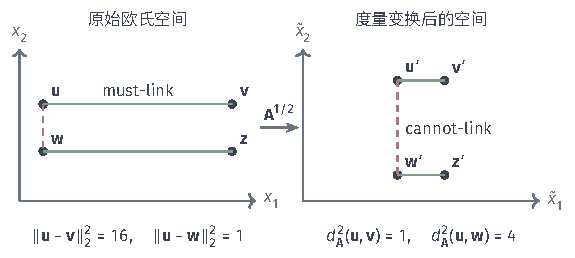
\includegraphics[width=97.331mm]{figures/04-classic-models/00-shared/tikz/clustering-metric-constraints/figure.pdf}
  \caption{度量如何改变成对关系的几何表达。四点为 $\bm{u}=(-2,0.5)$、$\bm{v}=(2,0.5)$、$\bm{w}=(-2,-0.5)$、$\bm{z}=(2,-0.5)$。实线连接 must-link 对，虚线连接 cannot-link 对。这里人为设定 $\bm{A}=\operatorname{diag}(1/16,4)$；右图的距离等于左图的 Mahalanobis 距离，不表示一次真实训练的结果。}
 \label{fig:clustering-metric-constraints}
\end{figure}

记在该度量下全数据的最大距离平方为
\[
 D_k=\max_{p,q\in\{1,\ldots,n\}}
 d_{\bm{A}_k}^2(\bm{x}_p,\bm{x}_q).
\]
对违反 must-link 的样本对，惩罚同时作用于两端所属簇；对违反 cannot-link 的样本对，惩罚其相对于本簇度量下最远样本对的接近程度。具体写为
\begin{align}
 f_M(i,j)
 &=\frac12\left[
 d_{\bm{A}_{c_i}}^2(\bm{x}_i,\bm{x}_j)
 +d_{\bm{A}_{c_j}}^2(\bm{x}_i,\bm{x}_j)\right]
 \mathbb{1}\{c_i\ne c_j\},\nonumber\\
 f_B(i,j)
 &=\left[D_{c_i}
 -d_{\bm{A}_{c_i}}^2(\bm{x}_i,\bm{x}_j)\right]
 \mathbb{1}\{c_i=c_j\}.
 \label{eq:clustering-mpck-penalty}
\end{align}
因此 cannot-link 惩罚非负，must-link 惩罚也不因交换样本对的书写顺序而改变。总目标为
\begin{equation}
 \begin{aligned}
 J={}&\sum_{k=1}^K\sum_{i\in C_k}
 \left[d_{\bm{A}_k}^2(\bm{x}_i,\bm{\mu}_k)
       -\log\det\bm{A}_k\right]\\
 &+\sum_{(i,j)\in M}w_{i,j}^{M}f_M(i,j)
  +\sum_{(i,j)\in B}w_{i,j}^{B}f_B(i,j).
 \end{aligned}
 \label{eq:clustering-mpck}
\end{equation}
权重均非负，每个无序约束对只计一次。负对数行列式阻止特征值趋零，但不能单独阻止矩阵某些方向无限放大；数据退化时仍需约束或正则。

\subsubsection{参数学习}

固定中心和度量时，对一个样本的各簇候选计算完整目标变化，包括几何、行列式及所有相关关系惩罚，再接受不增目标的变更。由于关系项耦合样本，单独比较到中心的距离不足以完成这项选择。

固定分配和度量时，约束项不含中心。对中心求导给出
\[
 2\bm{A}_k\sum_{i\in C_k}(\bm{\mu}_k-\bm{x}_i)=\bm{0},
 \qquad
 \bm{\mu}_k=\frac{1}{|C_k|}\sum_{i\in C_k}\bm{x}_i.
\]
同一簇共用的$\bm{A}_k$在驻点方程中消去，中心因而取普通簇内均值。若需按样本重要性加权，还要在目标中另加相应权重。

度量步可借助散布矩阵理解。令 $\bm{S}_k=\sum_{i\in C_k}(\bm{x}_i-\bm{\mu}_k)(\bm{x}_i-\bm{\mu}_k)^\top$。在固定当前最远样本对、且该样本对在更新后仍保持活跃的一个分支上，约束项写成 $\operatorname{tr}(\bm{A}_k\bm{P}_k)$，其中 $\bm{P}_k$ 汇总违反 must-link 的半权重差分外积，以及违反 cannot-link 的“最远对外积减约束对外积”。于是子目标为
\[
 \operatorname{tr}\bigl(\bm{A}_k(\bm{S}_k+\bm{P}_k)\bigr)
 -|C_k|\log\det\bm{A}_k.
\]
若 $\bm{S}_k+\bm{P}_k\succ0$ 且 $|C_k|>0$，其无约束驻点为
\begin{equation}
 \bm{A}_k=|C_k|(\bm{S}_k+\bm{P}_k)^{-1}.
 \label{eq:clustering-mpck-metric}
\end{equation}
这个驻点式适用于正定的调整散布及保持活跃的最远对分支；更新后需再次核对这两个条件。

保留 $D_k$ 对 $\bm{A}_k$ 的真实依赖时，它是有限个线性函数的最大值，故固定分配和中心的度量子问题是凸的，但通常分段光滑。可在 $\alpha\bm{I}\preceq\bm{A}_k\preceq\beta\bm{I}$、$0<\alpha<\beta$ 的固定域上求解，或使用保持正定且实际下降的优化步骤。对角度量进一步减少参数与矩阵计算。

各步在同一有下界的目标上不增，可推出目标值收敛。度量属于连续参数，即使簇分配不再变化，它也可能继续更新；有限分配数因此不足以证明有限轮停止。实际终止可结合目标和参数变化的容差，并明确空簇处理。

\subsubsection{理论分析}

\paragraph{表达能力}
学习度量能让不同方向采用不同的距离权重。例如，图\ref{fig:clustering-metric-constraints}中的固定矩阵让同一水平行的距离变小、上下两行的距离变大，因而可以保留由行位置决定的关系。若全部簇共享一个正定矩阵，坐标变换仍是可逆线性变换，最近中心区域仍由半空间形成，不能单靠这种共享度量解决完整同心圆的分组。

每簇不同的矩阵增加了另一种表达。冻结参数、按目标的单点几何项比较新点时，得分为
\[
 s_k(\bm x)=(\bm x-\bm\mu_k)^\top\bm A_k(\bm x-\bm\mu_k)
            -\log\det\bm A_k.
\]
两簇的得分差是二次函数，可以形成原空间线性中心无法表达的边界。取二维$\bm\mu_1=\bm\mu_2=\bm0$、$\bm A_1=4\bm I$、$\bm A_2=\bm I$，得分差为$3\lVert\bm x\rVert_2^2-\log16$。选择较小得分会按半径$\sqrt{\log16/3}$分开内外区域，因而能够准确区分半径为$1/2$和2的两圈。这个教学例说明候选增加了什么，并未保证少量关系监督能估计出这组参数。一般多弯曲分组也未必能用固定的两条二次得分表示；成对惩罚对训练对象的作用仍需另外计算。



\paragraph{收敛性}
若把中心限制在有界闭球内，并要求$\alpha\bm I\preceq\bm A_k\preceq\beta\bm I$、$0<\alpha<\beta$，连续参数域紧致；分配只有有限种，目标连续，故全局最小值存在。每一步若在同一目标上不增，目标值便收敛。连续度量仍可能无限次更新，因而有限分配数不能推出有限轮停止，也不能仅从目标值收敛推出参数达到驻点。固定分配和中心的度量子问题为凸问题，但交替求解整体仍非凸，没有上述条件自动给出的全局最优速率。

\paragraph{泛化性}
\begin{theorem}[MPCK-means在有界度量与独立验证下的期望几何风险界]
冻结参数后，采用前面定义的最小得分$\min_k s_k(\bm x)$评价新点。若$\lVert\bm X\rVert_2,\lVert\bm\mu_k\rVert_2\leq r$且各度量特征值位于$[\alpha,\beta]$，则该得分位于$[-d\log\beta,4\beta r^2-d\log\alpha]$，区间长度为$B=4\beta r^2+d\log(\beta/\alpha)$。对独立的$m$个同分布验证样本，以至少$1-\delta$的概率，
\[
 R=\mathbb E\min_k s_k(\bm X)
 \leq\frac1m\sum_{i=1}^m\min_k s_k(\bm X_i^{\mathrm{val}})
       +B\sqrt{\frac{\log(1/\delta)}{2m}}.
\]
\end{theorem}

这是有界损失的单候选Hoeffding结论。它控制冻结度量在新点上的几何得分，不包含未观测样本对的约束惩罚；后者还需规定新关系如何生成和评价。

\subsubsection{优化计算能力}

Xing 等通过相似与不相似样本关系学习 Mahalanobis 度量\scite{clust-xing2003}。这是先单独学习共享度量、再交给聚类算法的解耦方式。这样可以复用监督得到的几何结构，但共享度量仍假设所有簇使用同一种空间变换，后续算法也须与该度量兼容。

\subsubsection{小结}

MPCK-means让关系监督同时改变分配与比较几何，适合距离本身没有反映领域关系的情形。每簇独立度量增加了可调整的方向与尺度，也增加矩阵求解及监督需求；共享或对角形式减小这份负担，同时限制不同群组采用不同几何的能力。

监督还可以在另一个环节发挥作用：先单独学习共享度量再聚类，或修改关系图再求谱表示。这些路线没有联合优化MPCK的完整目标，后续分配也未必逐项满足输入关系。应按关系覆盖、错误类型及新点用途选择监督进入的位置，并检查额外参数是否得到足够支持。

\subsection{模型对比与总结}

关系和种子可以在不同环节减少无标签分组的歧义。COP-K-means直接排除违反must-link或cannot-link的分配，适合可靠且可满足的关系；关系相互冲突时，它可能没有可行结果。软约束改用违反代价保留可行搜索，但权重决定愿意付出多少距离损失来满足监督。Seeded K-means主要用标注记录确定初始中心，Constrained K-means还限制这些记录的后续归属，二者对标签的使用强度不同。

若原始距离本身不能体现监督关系，只限制分配仍会让几何与标签相互拉扯。MPCK-means让每簇度量与分配共同调整，允许不同群组采用不同方向和尺度；共享度量学习减少参数并可复用于其他算法，却要求所有群组接受同一变换。监督也可以直接改变谱图边权，但这会改变图偏好，并不逐项保证最终标签满足关系。

这些方法分别改变可行集合、初始化、几何或图关系。选择前要判断信号是否可靠、覆盖了哪些群组，以及额外度量参数是否有足够监督支持。报告几何目标和关系违反可以解释监督怎样进入拟合，独立参考标签或下游任务再检查这些改变是否带来预定用途。

\section{本章小结}
\label{sec:clustering-summary}

聚类通过结构假设定义群组。原型限定中心周围的相异度，邻域和图限定连接，网格与子空间限定相关区域，层次限定嵌套关系，概率模型限定生成成分。关系与种子监督再减少其中部分歧义。

算法求解与群组用途需要不同证据。目标下降和停止支持计算解释，训练外量化、密度、语义或决策结果支持使用结论；稳定性及零模型补充结构检验。粒度由$K$、密度阈值、带宽、截线或先验控制，均需随任务选择。

评价应先对应群组用途。留出量化误差检验数值压缩，预测对数密度检验生成拟合，独立参考标签检验指定语义，相对无聚类基线的下游损失检验使用收益。\term{轮廓系数}（silhouette coefficient）比较同簇与其他簇的距离，偏好相应的紧凑几何；\term{调整兰德指数}（adjusted Rand index, ARI）比较两份划分的共簇关系，并校正指定随机基准下的一致性\scite{clust-rousseeuw1987,clust-hubert1985}。它们提供不同证据，不能彼此替代。

为检查训练外的用途，可将数据分为\term{发现数据}（discovery data）与\term{验证数据}（validation data）。表示、尺度、相异度、候选和超参数在发现数据上确定，再冻结分配、匹配及指标规则用于验证；时间、地点或个体相关记录按未来使用单位隔离\scite{clust-ullmann2022}。稳定性检验扰动后的重复性，零模型检验结构是否超出指定基线；模拟比较需重跑完整发现流程，把选择过程也纳入基线。

第\ref{chap:dimensionality-reduction}章将学习低维表示，这会同时改变距离、密度和邻接。可视化提供探索线索，群组判断仍需在原始或经验证的表示上取得与用途对应的证据。

\paragraph{扩展阅读}
进一步阅读可围绕同一数据问题，分别写出几何分组与概率成分的定义、学习目标和新样本评价，比较不同假设怎样改变最终群组\scite{bishop2006,hastie2009}。

\chapter{降维}
\label{chap:dimensionality-reduction}

基因测量或文档向量可以包含成千上万个坐标，其中许多坐标却描述相近的变化。若能用较少的数值保留分析所需的信息，后续计算和解释就更容易展开。\term{降维}（dimensionality reduction）把观测$\bm{x}\in\mathbb{R}^{d}$转为表示$\bm{z}\in\mathbb{R}^{k}$，通常取$k\ll d$。压缩时需要先决定保留什么：方差、点间距离、邻域关系和生成因素各有用途，对后续预测、分组或解释的价值也需要分别检验。

维数很高还会增加覆盖数据空间的困难。把每个单位坐标区间划成十段，$d$维空间就有$10^d$个区域，有限样本很快不足以覆盖。这样的空间覆盖和统计估计困难统称\term{维数灾难}（curse of dimensionality）。降维只有在冗余、低维结构或任务信息确实可以提取时，才可能减少这部分负担；压缩本身不能保证有用信息仍被保留。

降维方法的发展也围绕这些不同的保留目标展开。20世纪初的PCA提取线性变化的主要方向，1950年代的MDS根据对象差异恢复坐标。1990年代的核PCA将方差分析带入非线性特征空间，2000年前后的Isomap与LLE从局部关系组织几何表示；2008年的t-SNE和2018年的UMAP则扩展了高维邻域的可视化方法\scite{dimScholkopf1998,dimTenenbaum2000}

在压缩、去噪和建模前处理时，PCA可以作为简单基线；探索局部邻域时，t-SNE与UMAP常用来安排便于观察的坐标。图上的分离提示了值得检验的关系，检验仍要使用原始表示和任务证据\scite{classic-decomposition-guide,dim-mcinnes2018umapsoftware}本章沿保留的信息展开：从线性组合及核特征中的全局变化，转向点间差异和局部关系，再讨论如何用低维因素解释观测的生成。

为比较这些方法，以下用$n$表示样本数，$\bm{X}\in\mathbb{R}^{n\times d}$与$\bm{Z}\in\mathbb{R}^{n\times k}$按行存放观测和低维表示，邻居数记为$q$，内在维数记为$m$。“表示”是变换结果的统称；几何或邻域坐标称为“嵌入”；参与生成但未被观测的量称为“潜变量”。第\ref{chap:classic-models-overview}章的共享建模机制为这些不同目标提供了共同背景。

\section{基于线性关系的降维}
\label{sec:dim-linear}

多个传感器若主要随同一个物理量变化，观测可能集中在一条直线附近；多个共同因素则可以对应一个低维线性子空间。线性投影$\bm{z}=\bm{W}^{\top}(\bm{x}-\bm{\mu})$提取沿该子空间的坐标，其中$\bm{W}\in\mathbb{R}^{d\times k}$为列正交的基矩阵，$\bm{\mu}$为中心，$\bm{W}\bm{W}^{\top}$是相应的正交投影算子。方向学得后，矩阵乘法就能编码新样本，每个坐标也对应原特征的一个线性组合。

线性组合还可以用于重构，而不要求编码是输入的线性函数。非负矩阵分解和稀疏编码都用基向量组合观测，新样本的系数却通常由约束优化取得；独立源分离还要使用协方差以外的统计信息。核PCA保留的则是核所定义的特征空间中的方差。因此，本节会分别说明线性关系作用于编码、生成还是映射后的特征，再据此判断各方法保留的信息与求解方式。

\subsection{主成分分析（PCA）}
\label{sec:dim-pca}

多个传感器测量同一个状态时，读数可能一起升降，把每个读数都保存下来会重复记录这部分共同变化。直接保留其中一个传感器，又舍弃了其余测量提供的信息。我们可以把读数组合为少数新坐标，并要求这些坐标尽量保留样本的变化。\term{主成分分析}（principal component analysis, PCA）选择方差最大的正交方向；在同一正交投影设定下，这些方向也使恢复原样本的平均平方误差最小。于是，保留投影后的方差与减小重构误差成为同一个求解问题。Pearson在1901年研究点集的最佳拟合直线与平面，Hotelling在1933年研究多元统计中的主成分，分别从几何拟合与变量变化说明了这一结构\scite{pearson1901pca,hotelling1933pca}

\subsubsection{模型结构}
\label{sec:dim-pca-structure}

比较投影方差之前，需要把共同中心与样本变化分开。减去样本均值后，暂以$\bm{X}$表示中心化数据，样本协方差为$\bm{S}=\bm{X}^{\top}\bm{X}/n$。分母$n$与最大似然的协方差约定一致；使用$n-1$会统一缩放特征值，主成分方向保持相同。

单位方向$\bm{w}$上的投影方差为$\bm{w}^{\top}\bm{S}\bm{w}$。为同时保留$k$个互相正交的变化方向，将它们组成$\bm{W}$，最大化这$k$个坐标的方差总和：
\begin{equation}
  \max_{\bm{W}^{\top}\bm{W}=\bm{I}_k}
      \operatorname{tr}(\bm{W}^{\top}\bm{S}\bm{W}),
  \qquad \bm{Z}=\bm{X}\bm{W}.
  \label{eq:dim-pca-variance}
\end{equation}
约束使$\bm{W}$的列构成候选$k$维子空间的一组正交基，迹目标衡量该子空间保留的总方差。这里比较的是子空间，每一列尚未规定为协方差特征向量。编码得到的得分$\bm{z}=\bm{W}^{\top}\bm{x}$则是样本在这组基下的坐标。

把得分沿基向量组合起来，重构为$\widehat{\bm{x}}=\bm{W}\bm{W}^{\top}\bm{x}$。原样本由投影与正交残差组成，勾股关系因而给出
\begin{equation}
  \lVert\bm{x}-\widehat{\bm{x}}\rVert_2^2
  =\lVert\bm{x}\rVert_2^2-\lVert\bm{W}^{\top}\bm{x}\rVert_2^2.
  \label{eq:dim-pca-pythagoras}
\end{equation}
对全部样本取平均时，右侧第一项与$\bm{W}$无关，第二项就是保留的总方差。因此，增大投影方差等价于减小平均平方重构误差，图\ref{fig:dim-pca-projection}显示了这一分解。新观测编码时使用训练均值中心化，重构时再加回该均值。

\begin{figure}[htbp]
  \centering
  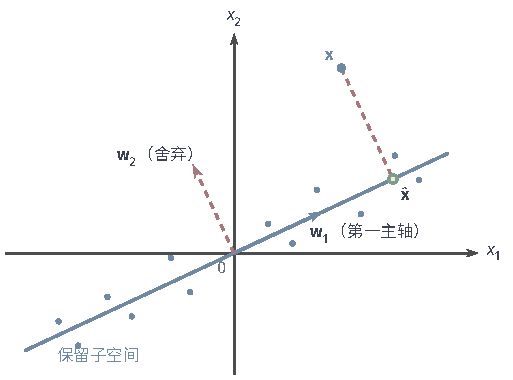
\includegraphics[width=86.935mm]{figures/04-classic-models/00-shared/tikz/dim-pca-projection/figure.pdf}
  \caption{二维到一维的正交投影示意。蓝色实线方向$\bm{w}_1$是保留的第一主轴，红色虚线方向$\bm{w}_2$是被舍弃的正交主轴。点$\bm{x}$投到$\widehat{\bm{x}}$，重构残差沿$\bm{w}_2$方向。图中散点为示意位置，未表示真实实验。}
  \label{fig:dim-pca-projection}
\end{figure}

\subsubsection{参数学习}
\label{sec:dim-pca-learning}

最优方向可以通过协方差的谱求出。在单位方向的约束目标中引入乘子$\lambda$，驻点方程为$\bm{S}\bm{w}=\lambda\bm{w}$，投影方差正好等于$\lambda$。按$\lambda_1\geq\cdots\geq\lambda_d\geq0$排序，前$k$个特征向量组成$\bm{V}_k$，其列称为\term{主成分方向}（principal component directions）。取$\bm{W}=\bm{V}_k$得到一个解析最优解；得分$\bm{X}\bm{V}_k$的经验协方差为$\operatorname{diag}(\lambda_1,\ldots,\lambda_k)$，所以这些得分不相关，统计独立还需要额外条件。

方向的唯一性需要分别看基矩阵、子空间与投影算子。一般最优$\bm{W}$是一组正交基，$\operatorname{span}(\bm{W})$是其张成的主子空间，$\bm{P}=\bm{W}\bm{W}^{\top}$是相应投影。若$\lambda_k>\lambda_{k+1}$，主子空间与投影唯一；子空间内部仍可以旋转，任意$k$阶正交矩阵$\bm{Q}$都使$\bm{W}\bm{Q}$给出同一投影，所有最优基可写成$\bm{V}_k\bm{Q}$。

坐标基的旋转却会改变各列及得分之间的关系。从$\bm{W}=\bm{V}_k$出发，若$\bm{Q}$混合不同特征值的方向，$\bm{W}\bm{Q}$的列一般不再是$\bm{S}$的特征向量，得分协方差$\bm{Q}^{\top}\operatorname{diag}(\lambda_1,\ldots,\lambda_k)\bm{Q}$一般也不再对角。因此，互不相关的主成分得分对应排序特征向量基$\bm{V}_k$，而非主子空间中的任意正交基。

如果进一步要求各列为排序后的特征向量，单特征值方向只差符号；所选范围内的重特征值允许在其重特征子空间中旋转。若$\lambda_k=\lambda_{k+1}$，重特征值跨过截断位置，最优主子空间和投影算子也可能不唯一。

实际计算通常对中心化数据作\term{奇异值分解}（singular value decomposition, SVD），写成$\bm{X}=\bm{U}\bm{\Sigma}\bm{V}^{\top}$。右奇异向量给出主方向，$\lambda_j=\sigma_j^2/n$，得分为$\bm{U}_k\bm{\Sigma}_k$。直接SVD无需显式形成$\bm{X}^{\top}\bm{X}$，可以避免条件数平方带来的数值困难。完整稠密分解约需$O(nd\min(n,d))$次运算，只求少数方向时还可使用截断算法；不同实现需要不同的矩阵和计算预算。

用同一批点比较不同方向，可以直接看出重构目标怎样选择主轴。图\ref{fig:dim-pca-objective}中，水平方向留下的平均平方残差为$0.8125$；改用SVD算出的第一主方向后，残差降为$0.25$。两图的样本、中心和坐标尺度都相同，变化只来自所保留的方向。

\begin{figure*}[tbp]
  \centering
  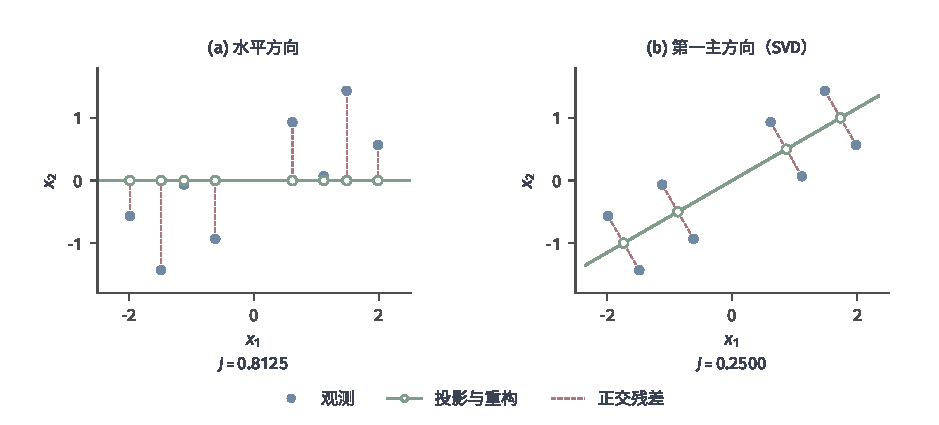
\includegraphics[width=159.000mm]{figures/04-classic-models/00-shared/matplotlib/dim-pca-objective/figure.pdf}
  \caption{PCA重构目标的数值对照。取八个无量纲点$(t,u)$，其中$t\in\{-2,-1,1,2\}$、$u\in\{-1/2,1/2\}$，统一逆时针旋转$30^\circ$；样本均值为零。蓝点为观测，绿线为保留方向，空心点为正交重构，红色虚线为残差；右图部分重构点重合。平均平方残差记为$J$，两个方向分别给出$0.8125$和$0.25$。第一主方向由这组数据的SVD实际计算，图中未人为指定拟合结果。}
  \label{fig:dim-pca-objective}
\end{figure*}

当$d\gg n$时，样本空间中的$n\times n$ Gram矩阵$\bm{X}\bm{X}^{\top}$更小。若$\bm{X}\bm{X}^{\top}\bm{u}_j=\sigma_j^2\bm{u}_j$且$\sigma_j>0$，右奇异向量可由$\bm{v}_j=\bm{X}^{\top}\bm{u}_j/\sigma_j$恢复。这仍是同一SVD；第\ref{sec:dim-kpca}节将沿样本空间计算引出核方法。

求出特征值后，可以衡量前$k$个方向保留的方差比例。\term{累计解释方差}（cumulative explained variance）定义为
\begin{equation}
  \eta_k=\frac{\sum_{j=1}^{k}\lambda_j}
                    {\sum_{j=1}^{d}\lambda_j}.
  \label{eq:dim-explained-variance}
\end{equation}
总方差非零时，可以按预先选择的比例确定$k$，也可以查看特征值随序号下降的碎石图。$85\%$、$95\%$等比例是经验阈值，并非预测信息的保证：低方差方向可能包含第\ref{sec:classification-lda-model}节的类别判别信息，高方差也可能来自量纲或背景干扰。是否标准化由特征单位和任务决定；服务于预测的维数选择应使用训练集内部的验证结果。

矩阵规模过大时，还可以近似求主子空间。随机化SVD先估计列空间，再分解较小的矩阵；增量PCA按批次更新子空间。二者以近似误差或特定更新规则换取内存与时间收益，评价时需要同时检查求解精度\scite{halko2011}

\subsubsection{理论分析}
\label{sec:dim-pca-theory}

\paragraph{表达能力}
PCA能否完整保留观测，取决于数据是否落在一个$k$维仿射子空间中。设观测$\bm X$有有限二阶矩，均值为$\bm\mu$、协方差为$\bm\Sigma_\star$，后者的有序特征值为$\lambda_1^\star\geq\cdots\geq\lambda_d^\star\geq0$。对任一秩$k$正交投影$\bm P$，重构残差的期望平方为$\operatorname{tr}((\bm I-\bm P)\bm\Sigma_\star)$。沿协方差特征方向分解这一量，保留最大的$k$项便得到
\begin{equation}
 \min_{\bm P}\mathbb E\lVert
   (\bm I-\bm P)(\bm X-\bm\mu)\rVert_2^2
   =\sum_{j>k}\lambda_j^\star.
 \label{eq:dim-pca-representation-error}
\end{equation}
右侧为零，恰好意味着观测以概率一落在所保留的仿射子空间中。数据只集中在子空间附近时，舍弃方差之和就是这一候选族无法消除的重构误差，增加求解精度不会减小它。

内在维数小并不足以使这个误差为零。例如在单位圆周上均匀取点，分布只沿一条曲线变化，协方差却为$\bm I_2/2$；任何一维PCA的期望重构误差都是$1/2$。若低秩信号再叠加独立、均值为零、协方差为$\tau^2\bm I_d$的观测噪声，任何秩$k$投影的残差中又至少包含$(d-k)\tau^2$的噪声方差。这里评价的是重构观测；恢复无噪声信号需要另换评价对象。低方差方向也可能承载类别信息，因此较小的重构误差本身不保证保留预测所需的信息。

\paragraph{收敛性}

固定数据上的最优重构可以由Eckart--Young低秩逼近定理说明\scite{eckart1936}下面将这一结果用于PCA的正交重构，再把它与估计总体子空间的问题分开。

在正交投影与平方误差设定下，前$k$维主子空间达到经验全局最优，最小误差等于舍弃特征值的总和。截断处的谱隙进一步决定投影是否唯一：

\begin{theorem}[PCA最优重构解的存在性与谱间隔下的唯一性]
  \label{thm:dim-pca-optimal}
  设$\bm{X}$已中心化，$1\leq k<d$，$\lambda_j$为$\bm{S}=\bm{X}^{\top}\bm{X}/n$按降序排列的特征值。则
  \[
    \min_{\bm{W}^{\top}\bm{W}=\bm{I}_k}
       \frac1n\lVert\bm{X}-\bm{X}\bm{W}\bm{W}^{\top}\rVert_F^2
       =\sum_{j=k+1}^{d}\lambda_j.
  \]
  前$k$个特征向量张成的子空间达到最小值。若$\lambda_k>\lambda_{k+1}$，最优投影算子$\bm{W}\bm{W}^{\top}$唯一，但子空间内的正交基不唯一。
\end{theorem}

\begin{proof}
在所有秩至多为$k$的矩阵中，截断SVD使平方Frobenius误差最小（参见\BookTheoremRef{thm:matrix-analysis-best-low-rank}{卷1《数学准备：计算、分析与几何》第5章“线性空间”第5.5.4节“秩约束下的矩阵逼近”}）。
截断SVD给出$\bm X\bm V_k\bm V_k^\top$，其平方误差为$\sum_{j>k}\sigma_j^2$；
除以$n$并代入$\lambda_j=\sigma_j^2/n$即得结论。
截断处的严格谱隙使主子空间与投影唯一，唯一的投影仍允许在其子空间中选择不同的正交基。
\end{proof}

迭代谱算法要逼近的是定理中的全局最优投影，可以用特征方程残差和方向正交误差检查数值精度。增加迭代可以改善求解误差；样本是否足以估计总体结构，则是下面的统计问题。

\paragraph{泛化性}
训练重构最优的子空间，仍可能在新样本上丢失更多变化。沿用期望风险记号，设$D_n$独立同分布于$P$，总体均值为$\bm\mu$、协方差为$\bm\Sigma_\star$。训练所得均值与投影为$\bar{\bm X}$、$\widehat{\bm P}$，新点的重构规则固定为
$\widehat r_n(\bm x)=\bar{\bm X}+\widehat{\bm P}(\bm x-\bar{\bm X})$。
其风险$R_n=\mathbb E_{\bm X\sim P}\lVert\bm X-\widehat r_n(\bm X)\rVert_2^2$中的新点独立于训练集。下面直接比较这一风险与最佳$k$维仿射重构，而不要求主方向估计唯一。

\begin{theorem}[PCA在有界观测下的期望重构风险界]
 \label{thm:dim-pca-risk}
 假设$\lVert\bm X-\bm\mu\rVert_2\leq r$几乎处处，$\bm S$是以样本均值中心化、分母为$n$的样本协方差。设$\widehat{\bm P}$为秩$k$正交投影，满足
 \[
 \operatorname{tr}(\bm S\widehat{\bm P})
 \geq\max_{\bm P\text{为秩}k\text{正交投影}}
       \operatorname{tr}(\bm S\bm P)-e_n,
 \qquad e_n\geq0.
 \]
 记$R_k^\star=\min_{\bm P}\operatorname{tr}((\bm I-\bm P)\bm\Sigma_\star)$。则
 \begin{equation}
  \mathbb E_{D_n}R_n
  \leq R_k^\star+\frac{2\sqrt{k}\,r^2}{\sqrt n}
          +\frac{(2\sqrt{k}+1)r^2}{n}
          +\mathbb E_{D_n}e_n.
  \label{eq:dim-pca-risk-bound}
 \end{equation}
\end{theorem}
\begin{proof}
将$\bm X-\bar{\bm X}$分成$\bm X-\bm\mu$与均值误差，独立新点的交叉项期望为零，得到
\[
 R_n=\operatorname{tr}((\bm I-\widehat{\bm P})\bm\Sigma_\star)
       +\lVert(\bm I-\widehat{\bm P})(\bar{\bm X}-\bm\mu)\rVert_2^2.
\]
设$\bm P_\star$为总体最优投影。在投影风险差中加入样本协方差，并使用经验最优性，有
\begin{equation}
 \begin{aligned}
 \operatorname{tr}((\bm P_\star-\widehat{\bm P})\bm\Sigma_\star)
 &\leq\operatorname{tr}((\bm P_\star-\widehat{\bm P})
                          (\bm\Sigma_\star-\bm S))+e_n\\
 &\leq2\sqrt{k}\,\lVert\bm S-\bm\Sigma_\star\rVert_F+e_n.
 \end{aligned}
 \label{eq:dim-pca-excess-risk}
\end{equation}
最后一步使用两个秩$k$投影的Frobenius范数至多各为$\sqrt k$。
令$\bm Y_i=\bm X_i-\bm\mu$及$\bm e=\bar{\bm X}-\bm\mu$，则
$\bm S=n^{-1}\sum_i\bm Y_i\bm Y_i^\top-\bm e\bm e^\top$。
独立性与$\lVert\bm Y_i\rVert_2\leq r$给出
\[
 \mathbb E\left\lVert\frac1n\sum_i\bm Y_i\bm Y_i^\top
                        -\bm\Sigma_\star\right\rVert_F
 \leq\frac{r^2}{\sqrt n},
 \qquad \mathbb E\lVert\bm e\rVert_2^2\leq\frac{r^2}{n}.
\]
因此$\mathbb E\lVert\bm S-\bm\Sigma_\star\rVert_F
\leq r^2/\sqrt n+r^2/n$。代入风险分解，并以$\lVert\bm e\rVert_2^2$控制均值项，得到结论。
\end{proof}

定理把总体重构拆成最佳线性近似误差、协方差与均值的估计误差，以及数值求解误差。精确谱分解使$e_n=0$；随机化SVD与增量近似应保留该项。风险界不需要谱隙，相近特征值对应的方向可以明显旋转，重构损失却只改变很少。若要估计方向本身，谱隙才成为另一项条件。

有界观测是本定理的明确条件，重尾或维数随样本量增长时需采用相应矩条件和估计方法。尖峰协方差模型与Marchenko--Pastur型谱极限说明样本谱可能偏离总体结构\scite{nadler2008,marchenko1967}这些参数或谱结论不能代替式\eqref{eq:dim-pca-risk-bound}所评价的新样本重构。奇异值阈值也应在指定噪声与损失条件下使用\scite{donoho2014threshold}

\subsubsection{优化泛化能力}

\paragraph{分离稀疏异常污染}
\label{sec:dim-robust-pca}

普通PCA以平方误差衡量重构，一小部分幅度很大的污染就可能拉动主方向。考虑固定摄像机拍摄的构造场景：背景基本不变，移动物体每帧只覆盖少量像素。把各帧排成观测矩阵$\bm{M}\in\mathbb{R}^{n\times d}$后，相似的背景可以用低秩矩阵$\bm{L}$表示，少量变化像素则放入稀疏矩阵$\bm{E}$。分别估计这两部分，可以让大幅度的局部变化留在扰动中，而不迫使背景子空间追随它们。这里的\term{鲁棒PCA}（robust PCA, RPCA）专指低秩加稀疏分解，稳健子空间估计还包括其他污染设定。

同时寻找低秩部分和稀疏部分时，直接最小化$\operatorname{rank}(\bm{L})+\lambda\lVert\bm{E}\rVert_0$存在组合困难。\term{主成分追踪}（principal component pursuit, PCP）用两个凸惩罚替代秩和非零元素数：
\begin{equation}
  \min_{\bm{L},\bm{E}}\
     \lVert\bm{L}\rVert_*+\lambda\lVert\bm{E}\rVert_1,
  \qquad \bm{M}=\bm{L}+\bm{E}.
  \label{eq:dim-pcp}
\end{equation}
核范数$\lVert\bm{L}\rVert_*=\sum_j\sigma_j(\bm{L})$鼓励较少的非零奇异值；$\lVert\bm{E}\rVert_1$为所有元素绝对值之和，鼓励较少的非零污染项。两个惩罚分别作用于整体秩结构与逐元素扰动。

\paragraph{表达能力}
低秩加稀疏模型可以精确表示“共享背景加少量任意幅度的像素污染”，前提是无污染矩阵确实低秩、污染确实只占少数位置。它不要求污染幅度小，却要求两部分能由结构区分。以$\bm e_i,\bm e_j$表示行、列空间中的坐标向量，取$\bm T=\bm e_i\bm e_j^\top$，它既是秩一矩阵，又只有一个非零元素；观测$\bm M=\bm T$既能解释为$(\bm L,\bm E)=(\bm T,\bm0)$，也能解释为$(\bm0,\bm T)$。只写低秩和稀疏，便无法判断哪一种是真实背景。

若还有稠密测量噪声，等式$\bm M=\bm L+\bm E$便不能同时把它解释成干净低秩信号与稀疏污染，需要允许剩余误差。整行损坏也不同于少量像素损坏，应按污染对象改用相应约束。

\paragraph{参数学习}
两个惩罚可以由\term{交替方向乘子法}（alternating direction method of multipliers, ADMM）分开求解，再通过重构约束协调。取惩罚参数$\rho>0$，引入与$\bm{M}$同形的$\bm{U}$作为缩放对偶变量，即拉格朗日乘子除以$\rho$。固定$\bm{U}$并略去无关常数，增广目标为
\[
  \lVert\bm{L}\rVert_*+\lambda\lVert\bm{E}\rVert_1
  +\frac{\rho}{2}
   \lVert\bm{M}-\bm{L}-\bm{E}+\bm{U}\rVert_F^2.
\]
固定$\bm{E}$更新$\bm{L}$，再用新$\bm{L}$更新$\bm{E}$，分别对应两种阈值运算。随后将尚未满足的重构误差加到$\bm{U}$，让下一轮继续校正约束偏差。从$\bm{U}^{(0)}=\bm{0}$开始时，一轮更新为
\begin{equation}
  \begin{aligned}
  \bm{L}^{(t+1)}&=\operatorname{SVT}_{1/\rho}
                  (\bm{M}-\bm{E}^{(t)}+\bm{U}^{(t)}),\\
  \bm{E}^{(t+1)}&=\mathcal{S}_{\lambda/\rho}
                  (\bm{M}-\bm{L}^{(t+1)}+\bm{U}^{(t)}),\\
  \bm{U}^{(t+1)}&=\bm{U}^{(t)}
                   +\bm{M}-\bm{L}^{(t+1)}-\bm{E}^{(t+1)}.
  \end{aligned}
  \label{eq:dim-rpca-admm}
\end{equation}
逐元素软阈值为$\mathcal{S}_{a}(u)=\operatorname{sign}(u)(|u|-a)_+$，$\operatorname{SVT}_{a}$则将同一运算作用于奇异值。模型中的$\bm{E}$代表稀疏扰动，迭代中的$\bm{U}$累积重构约束误差。为检查固定$\rho$下的停止条件，需要同时计算
\[
  \begin{aligned}
    r_{\mathrm{pri}}^{(t+1)}
      &=\lVert\bm{M}-\bm{L}^{(t+1)}-\bm{E}^{(t+1)}\rVert_F,\\
    r_{\mathrm{dual}}^{(t+1)}
      &=\rho\lVert\bm{E}^{(t+1)}-\bm{E}^{(t)}\rVert_F.
  \end{aligned}
\]
原始残差检查重构等式，对偶残差检查第二个子问题的变化是否仍破坏前一个子问题的平衡。两项均应低于按数据尺度设置的容差；迭代次数只是预算，不能代替这两项检查。

\paragraph{恢复与矩阵风险}
Candès等的精确恢复定理用不相干条件排除低秩信号集中在少数坐标的情形，并限制秩、污染比例与随机支持。满足后面定理\ref{thm:dim-rpca-matrix-risk}的条件时，PCP能恢复两部分，而不只是找到一个满足重构等式的分解\scite{candes2011rpca}。

\begin{theorem}[随机污染支持下的PCP恢复与矩阵风险]
 \label{thm:dim-rpca-matrix-risk}
 设$\bm M=\bm L_0+\bm E_0\in\mathbb R^{n\times d}$，
 $n_{\max}=\max(n,d)\geq2$、$n_{\min}=\min(n,d)$。
 固定秩$r_L$的$\bm L_0=\bm U\bm\Lambda\bm V^\top$，其奇异向量满足
 \[
 \begin{gathered}
 \max_i\lVert\bm U^\top\bm e_i\rVert_2^2\leq\mu r_L/n,
 \qquad
 \max_j\lVert\bm V^\top\bm e_j\rVert_2^2\leq\mu r_L/d,\\
 \lVert\bm U\bm V^\top\rVert_\infty\leq\sqrt{\mu r_L/(nd)}.
 \end{gathered}
 \]
 $\bm e_i$为相应空间的坐标向量，矩阵无穷范数在此为元素绝对值的最大值。
 污染符号与幅度固定，支持$\Omega$在所有含$s$个位置的子集中均匀抽取。
 存在绝对正常数$\rho_r,\rho_s,c$，使当
 \[
 r_L\leq\rho_r n_{\min}/[\mu(\log n_{\max})^2],
 \qquad s\leq\rho_s nd
 \]
 时，式\eqref{eq:dim-pcp}取$\lambda=1/\sqrt{n_{\max}}$，其全局解以至少$1-c n_{\max}^{-10}$的概率精确恢复$\bm L_0,\bm E_0$。
 若还知$|L_{0,ij}|\leq B$，将恢复矩阵逐元素截到$[-B,B]$得到$\widetilde{\bm L}$，则
 \begin{equation}
  \mathbb E_\Omega\frac{\lVert\widetilde{\bm L}-\bm L_0\rVert_F^2}{nd}
  \leq4B^2c n_{\max}^{-10}.
  \label{eq:dim-rpca-matrix-risk}
 \end{equation}
\end{theorem}
精确恢复的概率结论来自Cand\`es等的PCP定理\scite{candes2011rpca}。风险式在成功事件上为零，失败事件上每个元素的平方误差至多为$4B^2$，所以直接乘以失败概率即可。这里的随机性是当前矩阵中的污染支持，结论评价整矩阵恢复；PCP未学习一个处理独立新帧的共享编码器，不能将这个风险改称新帧重构风险。有限轮ADMM的求解误差也未包含在精确全局解结论中。

\paragraph{支持稠密测量噪声}
少量像素污染之外，每个像素还可能都有幅度较小的测量误差。这时精确等式会迫使低秩信号或稀疏污染吸收这部分误差。稳定PCP改为允许$\lVert\bm{M}-\bm{L}-\bm{E}\rVert_F\leq\delta$，用$\delta$限制剩余稠密误差的总量。它放松了重构约束，前面的无噪声精确恢复结论不能直接沿用。

\paragraph{支持成组的异常污染}
若整帧损坏，异常会占据观测矩阵的一整行，逐元素稀疏便不再准确描述污染方式。可以对污染矩阵按行施加组稀疏约束，让整条记录共同进入异常部分。视频背景、遮挡和传感器异常应据此区分局部像素污染与整条记录污染；约束改变后，两部分可识别的条件也需要重新检查。

\paragraph{利用已知子空间方向}
若已经知道部分背景方向，完全从观测重新寻找子空间会舍弃这项信息。侧信息变体把已知子空间特征写入分解的约束或表示，帮助限定仍需估计的信号方向\scite{dimChiang2016side}。收益取决于侧信息是否准确；错误方向也可能限制本来需要的信号，因而应连同其来源和误差一起检查。

\subsubsection{优化解释能力}

\label{sec:dim-sparse-pca}

普通PCA会综合全部坐标，即使只提取一个成分，也可能需要读取几乎所有变量。以基因表达分析为例，一个成分若由数千个基因以很小的权重共同组成，就不容易看出哪一小组基因解释了这项变化。\term{稀疏PCA}（sparse PCA）限制载荷中的非零项，把少量变量的要求与重构目标一同求解。它可能牺牲部分解释方差，换取更容易辨认和测量的变量组合；在普通PCA求解后直接删掉小载荷，通常不能得到这一受约束问题的最优解。Zou、Hastie与Tibshirani在2006年用回归式矩阵分解把成分提取与变量选择结合，并讨论基因表达等高维数据\scite{zou2006spca}其目标写为
\begin{equation}
  \begin{aligned}
  \min_{\bm{A},\bm{B}}\quad&
    \lVert\bm{X}-\bm{X}\bm{B}\bm{A}^{\top}\rVert_F^2
    +\lambda_1\sum_{j=1}^{k}\lVert\bm{b}_j\rVert_1
    +\lambda_2\lVert\bm{B}\rVert_F^2,\\
  \text{约束}\quad&\bm{A}^{\top}\bm{A}=\bm{I}_k.
  \end{aligned}
  \label{eq:dim-sparse-pca}
\end{equation}
在此目标中，$\bm{A},\bm{B}\in\mathbb{R}^{d\times k}$，$\bm{b}_j$是$\bm{B}$第$j$列，$\lambda_1,\lambda_2\geq0$。$\bm{B}$给出编码载荷，$\bm{A}$给出重构方向；$\ell_1$惩罚促使载荷稀疏，平方惩罚缓解相关变量造成的数值不稳定。

\paragraph{表达能力}
这一定义约束的是编码载荷$\bm B$，重构方向$\bm A$仍可使用全部变量。精确重构要求$\bm A\bm B^\top\bm x=\bm x$在数据支持上成立，因此数据必须落在$\bm A$张成的至多$k$维空间中。若数据只在$k$个原坐标上变化，取$\bm A=\bm B$为这些坐标向量，就能以稀疏载荷精确重构。

稀疏载荷也能编码某些稠密方向。设$\bm x=t\bm v$、$\lVert\bm v\rVert_2=1$，且第$j$个分量$v_j\ne0$。以$\bm e_j$表示第$j$个坐标向量，取$\bm A=\bm v$、$\bm B=\bm e_j/v_j$，只读取第$j$个变量便恢复$t$，再用$\bm A$重构整条直线。若$v_j$很小，这种编码需要较大的载荷幅度，也会放大该变量中的测量误差。额外幅度限制可能排除这一表示。无论载荷是否稀疏，重构仍落在一个固定线性子空间，式\eqref{eq:dim-pca-representation-error}仍给出其平方重构误差的下限。

\paragraph{参数学习}
惩罚目标未必会选择前述精确表示，因而需要按实际目标求解。交替求解时，固定$\bm{A}$，可以将$\bm{X}$分到$\bm{A}$的列空间与正交补：
\[
  \lVert\bm{X}-\bm{X}\bm{B}\bm{A}^{\top}\rVert_F^2
  =\lVert\bm{X}\bm{A}-\bm{X}\bm{B}\rVert_F^2
   +\lVert\bm{X}(\bm{I}-\bm{A}\bm{A}^{\top})\rVert_F^2.
\]
第二项与$\bm{B}$无关，所以编码载荷可以按列求弹性网回归。转而固定$\bm{B}$，需要最大化$\operatorname{tr}(\bm{A}^{\top}\bm{X}^{\top}\bm{X}\bm{B})$，这是寻找最佳正交对齐的Procrustes问题，可由SVD求解。交替更新通常得到局部解，初始化与惩罚强度的敏感性需要检查。

稀疏载荷让变量组合更容易辨认，同时也改变了得分之间的关系。$\bm{B}$各列通常不正交，得分方差可能重叠，因此各成分方差之和不能直接作为标准PCA式的解释方差。基因表达和文本等应用需要同时评价稀疏程度、重构效果与跨样本稳定性。

\paragraph{泛化性}
稀疏PCA不能原样套用正交PCA的风险式，因为$\bm A\bm B^\top$一般不是正交投影。仍可复用协方差比较：已知总体零均值时，令$\bm Q=(\bm I-\bm A\bm B^\top)^\top(\bm I-\bm A\bm B^\top)$，总体重构误差就是$\operatorname{tr}(\bm Q\bm\Sigma_\star)$。若抽样前另规定$\lVert\bm B\rVert_F\leq b$，则$\lVert\bm Q\rVert_F\leq\sqrt d(1+b)^2$；再结合有界观测下$\mathbb E\lVert\bm S-\bm\Sigma_\star\rVert_F\leq r^2/\sqrt n$，便能按定理\ref{thm:dim-pca-risk}的两次偏差比较方式控制风险。式\eqref{eq:dim-sparse-pca}的惩罚须同时除以$n$，在经验与总体目标中保持相同。均值也由样本估计时，还需增加均值误差；这组条件不会由载荷稀疏自动成立。

\subsubsection{优化计算能力}

持续接收新帧时，静态PCP要处理不断增长的矩阵，历史观测的存储与反复分解会增加负担。在线变体改为随观测到达更新子空间及污染估计\scite{dimFeng2013orPca}。它们需要规定保留哪些历史信息、怎样允许子空间变化及何时更新，静态矩阵的恢复结论不能自动解释整个流式过程。

\subsubsection{支持响应监督的降维场景}

用于预测时，方差较大的方向未必含有响应信息。例如，传感器读数可能主要随环境温度变化，待预测的状态却只体现为一个变化较小的坐标。这时需要改变方向的评价目标，而不只是增加PCA的成分数。第\ref{sec:regression-regularization}节的PCR按输入方差选成分，可能先删掉这个坐标；PLS让响应参与构造方向，第\ref{sec:classification-lda-model}节的线性判别分析则比较类间变化与类内变化。它们与PCA共享线性表示形式，选择方向的目标却不同。

Li在1991年提出的切片逆回归沿另一条路线，观察不同响应范围下的输入均值怎样改变，即利用$\mathbb{E}[\bm{x}\mid y]$寻找有效方向\scite{li1991sir}。它不直接寻找输入方差最大的轴；相应线性与非退化条件决定哪些响应方向能由条件均值显示，对称响应可能使这些均值不变而遗漏有关方向。

监督降维组合特征形成新方向，特征选择保留原坐标子集，两者可以共同使用。响应参与后，表示学习也增加了监督拟合与选择的环节。比较预测收益时，应将方向学习、特征选择和预测器都放在训练折内，以相同下游任务比较无监督表示、监督表示和不降维基线。

\subsubsection{小结}
\label{sec:dim-pca-summary}

PCA用一组共享线性方向压缩输入，并按平方重构目标选择保留的变化。维数决定压缩程度，变量尺度决定不同测量怎样参与比较；大幅度异常记录也可能改变主要方向。保留较多方差适合重构，却不必保留预测所需的低方差信息。

变量解释与异常污染需要不同调整。稀疏PCA让编码只读取少量变量，换取更容易辨认的组合，同时改变求解与成分方差的计算。低秩加稀疏的RPCA则把局部污染与共享信号分开，代价是更强的结构区分条件和迭代矩阵计算。前者限制载荷，后者改变观测分解，不能相互替代。

若表示服务于有监督预测，方向选择还应对应响应信息，可比较PLS、判别投影或切片逆回归等目标。若需解释测量噪声及潜变量不确定性，第\ref{sec:dim-ppca}节的概率模型提供另一种假设。选择时应先确认需要解释的是变量、污染、预测关系还是观测生成，再评价相应代价。

\subsection{典型相关分析（CCA）}
\label{sec:dim-cca}

同一对象可以有两组测量，例如图像特征与对应文字特征。分别做PCA保留的是各侧最大的变化，却未必是两侧共有的内容。用一个构造例子看这一区别：设$S,U,V$是互相独立、均值为零且方差有限的实值随机变量，$S$表示共同变化，$U,V$表示各侧独有的变化。两组观测为$(S,U)$与$(S,V)$，并令$U,V$的方差都大于$S$。按总体协方差各取一个PCA主成分时，两侧会分别选到$U,V$，丢掉共同的$S$。\term{典型相关分析}（canonical correlation analysis, CCA）改为选择两侧得分相关系数最大的投影；当$S$的方差非零时，两侧选取$S$就得到总体相关系数1。Hotelling的经典工作建立了这一双视图分析框架\scite{hotelling1936cca}。

\subsubsection{模型结构}
\label{sec:dim-cca-structure}

将成对观测中心化，记$\bm{x}\in\mathbb{R}^{d_x}$、$\bm{y}\in\mathbb{R}^{d_y}$，两侧协方差为$\bm{\Sigma}_{xx}$、$\bm{\Sigma}_{yy}$，交叉协方差为$\bm{\Sigma}_{xy}=\mathbb{E}[\bm{x}\bm{y}^{\top}]$。用同一批配对样本估计这些矩阵后，第一对方向按投影相关系数选择：
\begin{equation}
  \max_{\bm{w}_x,\bm{w}_y}
  \frac{\bm{w}_x^{\top}\bm{\Sigma}_{xy}\bm{w}_y}
  {\sqrt{\bm{w}_x^{\top}\bm{\Sigma}_{xx}\bm{w}_x}
   \sqrt{\bm{w}_y^{\top}\bm{\Sigma}_{yy}\bm{w}_y}}.
  \label{eq:dim-cca-correlation}
\end{equation}
相关系数只有在两侧投影方差均非零时有定义。缩放方向不改变相关性，因此可以令两侧方差均为$1$，将求解转为最大化交叉协方差。

图\ref{fig:dim-cca-shared}用两个视图比较方差与共有信息。各自方差最大的坐标$u$、$v$相互独立，较小方差的坐标却同为$t$，所以PCA与CCA会选择不同方向。此比较保留原坐标的方差；逐坐标标准化改变方差结构，也会改变PCA选择。

\begin{figure*}[!ht]
  \centering
  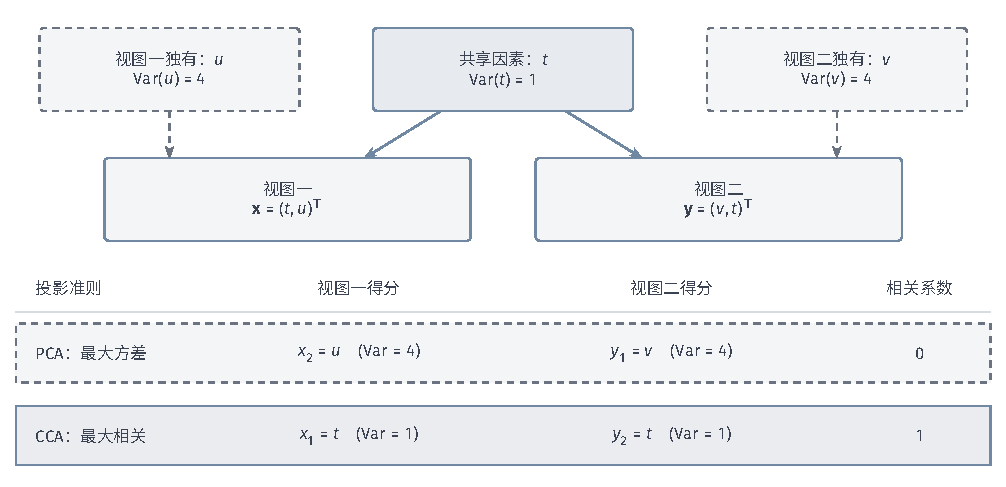
\includegraphics[width=169.000mm]{figures/04-classic-models/00-shared/tikz/dim-cca-shared/figure.pdf}
  \caption{CCA提取共有变化的构造例子。设$t,u,v$相互独立且均值为零，方差依次为$1,4,4$；两视图为$\bm{x}=(t,u)^\top$和$\bm{y}=(v,t)^\top$。实线连接共享因素，虚线连接各视图独有因素。各保留一维时，PCA选择$u,v$，CCA选择$t,t$，对应相关系数分别为$0$和$1$。箭头表示坐标构造关系，图中结论针对给定总体，不是样本拟合结果。}
  \label{fig:dim-cca-shared}
\end{figure*}

提取多对得分时，要求同一视图内$\bm{W}_x^{\top}\bm{\Sigma}_{xx}\bm{W}_x=\bm{I}_k$、$\bm{W}_y^{\top}\bm{\Sigma}_{yy}\bm{W}_y=\bm{I}_k$，使各得分方差为一且互不相关。这是协方差度量下的正交，原坐标中的方向未必欧氏正交。跨视图得分协方差可对角化为$\operatorname{diag}(\rho_1,\ldots,\rho_k)$，可识别的方向对数则同时受维数、样本秩与交叉协方差秩限制。

\subsubsection{参数学习}
\label{sec:dim-cca-learning}

两侧协方差正定时，可以先白化，使每侧协方差变成单位阵。白化后的交叉协方差及其SVD为
\[
  \bm{K}=\bm{\Sigma}_{xx}^{-1/2}
               \bm{\Sigma}_{xy}\bm{\Sigma}_{yy}^{-1/2},
  \qquad
  \bm{K}=\bm{U}\bm{D}\bm{V}^{\top}.
\]
令$\bm{a}=\bm{\Sigma}_{xx}^{1/2}\bm{w}_x$、$\bm{b}=\bm{\Sigma}_{yy}^{1/2}\bm{w}_y$，方差约束成为单位范数约束，目标成为$\max\bm{a}^{\top}\bm{K}\bm{b}$。取$\bm{K}$的首对左右奇异向量，就达到最大奇异值；多对方向由相应奇异向量依次取得：
\begin{equation}
  \bm{W}_x=\bm{\Sigma}_{xx}^{-1/2}\bm{U}_k,\qquad
  \bm{W}_y=\bm{\Sigma}_{yy}^{-1/2}\bm{V}_k,
  \label{eq:dim-cca-svd}
\end{equation}
$\bm{D}$的前$k$个对角元给出典型相关系数。实现白化时，可以使用Cholesky分解和三角求解，避免显式形成逆矩阵。

这一求解也可写成广义特征值问题。约束驻点满足$\bm{\Sigma}_{xy}\bm{w}_y=\rho\bm{\Sigma}_{xx}\bm{w}_x$及另一侧的对称方程，消去$\bm{w}_y$后得到
\[
  \bm{\Sigma}_{xy}\bm{\Sigma}_{yy}^{-1}
       \bm{\Sigma}_{yx}\bm{w}_x
  =\rho^2\bm{\Sigma}_{xx}\bm{w}_x.
\]


\subsubsection{理论分析}

\paragraph{表达能力}
CCA寻找的是两侧能用线性得分表达的共同变化。两侧协方差正定时，白化交叉协方差$\bm K=\bm\Sigma_{xx}^{-1/2}\bm\Sigma_{xy}\bm\Sigma_{yy}^{-1/2}$的奇异值$\rho_1\geq\rho_2\geq\cdots$就是可达的典型相关系数。对标准化得分$U,V$，有$\mathbb E(U-V)^2=2(1-\rho)$；因此$\rho=1$当且仅当两侧得分以概率一相同。前$k$对方向能保留$k$项最强的线性共有变化。各对标准化得分的均方差分别为$2(1-\rho_j)$，所以这一目标也直接给出了尚未匹配的共有变化。本节开头共享变量$S$的例子满足$\rho_1=1$，所以这一误差为零；各侧独有的$U,V$却无需保留。

线性得分可能完全看不到非线性依赖。例如$X\sim\mathcal N(0,1)$、$Y=X^2-1$时，$\mathbb E[XY]=0$，一维CCA的最大相关系数为零，但$Y$由$X$确定。把$X^2-1$纳入第一侧特征后才有可能匹配这一关系。这解释了核CCA扩展候选特征的作用；能否表达具体依赖仍取决于所选核，相关性目标也不保证恢复各视图的全部信息。


\paragraph{收敛性}
当两侧协方差正定时，白化把约束变为单位球面或正交列约束，可行集紧致，最大值存在。式\eqref{eq:dim-cca-svd}的SVD直接给出全局解；最大相关系数唯一，但对应方向只有在相应奇异值单一时才除符号外唯一。重奇异值允许在其子空间中旋转。协方差奇异时，应先限制到有正方差的支持空间；加入正则化则改变了原约束。迭代SVD的速度由具体求解器和奇异值间隔决定，CCA目标本身没有一个独立于谱间隔的统一迭代次数。

\paragraph{泛化性}
CCA的训练相关性可能很高，但新的一对观测不一定仍沿相同方向共同变化。可用总体标准化投影的均方差评价这一任务：对方向$\bm a,\bm b$，令
\[
 R(\bm a,\bm b)
 =\frac12\mathbb E\left(
 \frac{\bm a^\top\bm X}{\sqrt{\bm a^\top\bm\Sigma_{xx}\bm a}}
 -\frac{\bm b^\top\bm Y}{\sqrt{\bm b^\top\bm\Sigma_{yy}\bm b}}
 \right)^2
 =1-\rho(\bm a,\bm b).
\]
均值在此设为已知的零，$\rho$为式\eqref{eq:dim-cca-correlation}的总体相关系数。方向缩放不改变风险，所以可取两方向的欧氏范数为一。

\begin{theorem}[CCA在协方差非退化与扰动受控条件下的期望对齐风险界]
 \label{thm:dim-cca-risk}
 设$n$对观测独立同分布，已知总体均值为零，
 $\lVert(\bm X^\top,\bm Y^\top)^\top\rVert_2\leq r$几乎处处。
 记总维数为$q=d_x+d_y$，假设两侧总体协方差的最小特征值均至少为$v>0$。
 用已知零均值的经验二阶矩计算$\widehat\rho_n$，学习器的输出满足
 $\widehat\rho_n(\widehat{\bm a},\widehat{\bm b})
 \geq\sup_{\bm a,\bm b}\widehat\rho_n(\bm a,\bm b)-e_n$。
 对$0<\delta<1$，令
 \[
 \zeta_n=q r^2\sqrt{\frac{2\log(2q^2/\delta)}n}.
 \]
 若$\zeta_n\leq v/2$，则以至少$1-\delta$的训练抽样概率，
 \begin{equation}
 R(\widehat{\bm a},\widehat{\bm b})
 \leq\inf_{\bm a,\bm b}R(\bm a,\bm b)
       +\frac{8\zeta_n}{v}+e_n.
 \label{eq:dim-cca-risk}
 \end{equation}
\end{theorem}
\begin{proof}
对联合二阶矩的$q^2$个元素用Hoeffding界与并集界，得到全矩阵算子误差至多$\zeta_n$。两侧投影方差至少为$v$，经验方差至少为$v/2$。分子协方差的扰动不超过$\zeta_n$；将分母的两个方差逐项替换，并使用$|\rho|\leq1$，得到全体方向上的
$|\widehat\rho_n-\rho|\leq4\zeta_n/v$。
总体最优方向与经验选中方向各承担一次这一偏差，再加经验求解误差，即得结论。
\end{proof}

这里的风险是新配对观测的共有变化损失，概率界覆盖训练后选择的方向；它并未评价某一视图独有的信息。已知均值的设定省去了均值估计项，实际样本中心化需另外控制该项。协方差接近奇异时，分母使界变差，这也解释了小样本高维CCA的风险；加入正则项可以稳定分母，同时改变比较的风险。核CCA及深度CCA还需控制所选变换的复杂度，不能直接沿用固定线性方向的维数$q$。

\subsubsection{优化表达能力}

两侧共有的信息未必表现为线性相关。前面$Y=X^2-1$的例子中，只有把平方变化纳入候选特征，才可能匹配这一依赖。核CCA先固定两侧核映射，再在特征空间中匹配相关性；深度CCA则把两侧变换也纳入训练\scite{andrew2013dcca}。固定核预先规定哪些依赖可进入表示；联合学习变换使表示随数据调整，同时增加参数拟合与验证的成本。学习后的参数映射可用前向计算编码新样本，核形式则仍需按训练样本展开计算。

\subsubsection{优化泛化能力}

每侧变量数接近或超过配对样本数时，样本协方差可能奇异，前面的白化和求逆就不能按满秩形式执行。可以只在非零方差子空间中求解，或分别加$\lambda_x\bm{I}$、$\lambda_y\bm{I}$进行正则化。正则化改变了归一化度量，训练相关系数因而需要配合留出配对样本的相关性一起评价。

\subsubsection{小结}
\label{sec:dim-cca-summary}

CCA适合从配对观测中提取共有变化，相关性目标与单侧方差目标不同。某一视图独有却重要的信息可能不被保留，相关性也不能单独说明因果关系；使用前要判断两侧是否确实存在希望保留的共同内容。

样本少而维数高时，正则化稳定两侧方差的归一化，同时改变方向选择。共有关系非线性时，核CCA先规定特征映射，深度CCA再将两侧变换纳入训练。后一类方法增加表达与参数学习的自由度，也增加拟合成本；训练相关性应配合未用于拟合的配对观测检验，不能只用更大的训练值选择模型。

\subsection{独立成分分析（ICA）}
\label{sec:dim-ica}

两个麦克风同时录到两个人的声音，每条记录都是两个声源的不同比例混合。PCA可以找出变化较大、彼此不相关的方向，却没有理由让这些方向恰好对应两个说话人。协方差为零只排除了线性相关，例如$X\sim\mathcal{N}(0,1)$时，$X$与$X^2$的协方差为零，后者却完全由前者确定。\term{独立成分分析}（independent component analysis, ICA）进一步假设源信号独立，利用非高斯分布中的信息寻找解混方向，用于说话人分离、脑电活动分析和眼动伪迹分离等任务\scite{comon1994ica}这些假设决定能否识别声源；去相关本身并不能完成分离。

信息论提供了另一种减少分量依赖的准则。Bell与Sejnowski在1995年研究非线性网络中的信息传递，推导出利用协方差以外统计信息的学习规则，并讨论未知混合语音的分离和未知回声的消除\scite{bell1995infomax}这类问题称为盲信号处理，因为混合或传播过程未知；对源信号的结构仍需作出假设。

\subsubsection{模型结构}
\label{sec:dim-ica-structure}

为说明解混关系，先取中心化、无噪声且源数等于观测通道数的模型：
\begin{equation}
  \bm{x}=\bm{A}\bm{s},\qquad
  \bm{z}=\bm{W}^{\top}\bm{x},\qquad
  \bm{W}^{\top}=\bm{A}^{-1}.
  \label{eq:dim-ica-model}
\end{equation}
混合矩阵$\bm{A}\in\mathbb{R}^{d\times d}$可逆，源$\bm{s}$的分量相互独立。此处$\bm{W}$的列存放解混方向，所以$\bm{W}=\bm{A}^{-\top}$。若将$\bm{A}^{-1}$直接称为解混矩阵，则编码用它左乘观测；两种记法描述同一运算。

\subsubsection{参数学习}
\label{sec:dim-ica-learning}

存在密度时，可以比较解混分量的联合分布与边际乘积，用KL散度衡量剩余依赖。写成熵的形式为
\[
  I(z_1,\ldots,z_d)
  =\sum_{j=1}^{d}h(z_j)-h(\bm{z}),
\]
$h$为微分熵，上式要求各项有定义；散度为零恰好对应分量独立。也可以在单位方差约束下寻找非高斯方向，例如最大化负熵$J(z)=h(g)-h(z)$，其中$g$与$z$均值、方差相同且服从高斯分布。独立量相加趋向高斯提供了分离的直觉，具体对比量在有限线性组合中的性质仍需检验，不能直接由中心极限定理得到严格单调性。

指定各源密度$p_j$后，还可以按观测似然估计解混方向。变量替换同时改变密度和体积，得到
\begin{equation}
  \ell(\bm{W})
  =n\log|\det\bm{W}|
   +\sum_{i=1}^{n}\sum_{j=1}^{d}
        \log p_j(\bm{w}_j^{\top}\bm{x}_i).
  \label{eq:dim-ica-likelihood}
\end{equation}
行列式项是解混Jacobian对体积的校正。互信息、非高斯性与似然从不同角度利用分布信息；近似对比函数或错误源密度会改变目标，得到的方向也可能不同。

求独立方向之前，通常先去除协方差中的尺度和相关性。\term{白化}（whitening）将协方差变成单位阵：若$\bm{S}=\bm{V}\bm{\Lambda}\bm{V}^{\top}$且保留特征值为正，取$\widetilde{\bm{x}}=\bm{\Lambda}^{-1/2}\bm{V}^{\top}\bm{x}$。源方差规范为$1$后，白化空间中的混合矩阵正交，剩下的是方向选择。

图\ref{fig:dim-ica-whitening}给出白化仍未分离源的例子。左图协方差已为单位阵，但$x_1$接近边缘时，$x_2$允许的区间随之改变，两个分量仍依赖。旋转到右图源坐标后，均匀方形的联合分布才分成两个一维均匀分布。旋转前后的协方差相同，需要更完整的分布信息选择方向。

\begin{figure}[!ht]
  \centering
  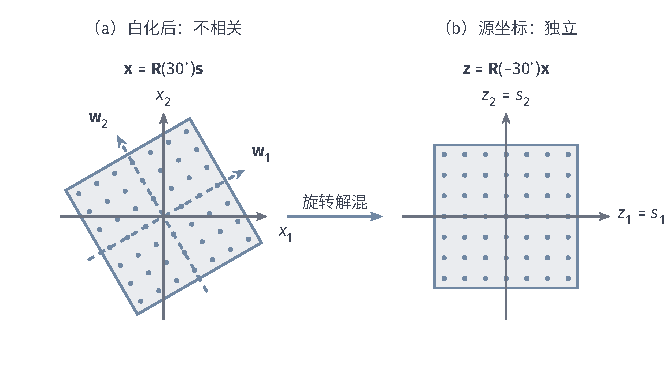
\includegraphics[width=112.000mm]{figures/04-classic-models/00-shared/tikz/dim-ica-whitening/figure.pdf}
  \caption{白化与独立源恢复的区别。设$s_1,s_2$独立且均服从$\mathcal{U}[-\sqrt3,\sqrt3]$，$\bm{R}(\theta)$为逆时针旋转矩阵。左图为$\bm{x}=\bm{R}(30^\circ)\bm{s}$，右图为逆旋转恢复的$\bm{s}$；两者协方差均为$\bm{I}_2$，只有右侧所示坐标对应独立源。实线轮廓为总体支持域，圆点为确定性格点，虚线箭头为解混方向。图为无量纲构造示意，未运行ICA优化；该方形解混本身不减少维数。}
  \label{fig:dim-ica-whitening}
\end{figure}

FastICA用光滑非二次函数$G$构造非高斯性对比量。单位方向$\bm{u}$在白化数据上产生方差为$1$的投影$\bm{u}^{\top}\widetilde{\bm{x}}$，可以将其与标准高斯变量$\nu$比较：
\begin{equation}
  J_G(\bm{u})
  =\left[
    \mathbb{E}G(\bm{u}^{\top}\widetilde{\bm{x}})
    -\mathbb{E}G(\nu)
  \right]^2,
  \qquad \lVert\bm{u}\rVert_2=1.
  \label{eq:dim-fastica-contrast}
\end{equation}
该目标近似前述负熵，其性质取决于$G$的选择。令$g=G'$；括号内的差非零、且期望与微分可交换时，$J_G$的球面驻点满足$\mathbb{E}G(\bm{u}^{\top}\widetilde{\bm{x}})$的约束驻点方程
\[
  \bm{a}(\bm{u})
  :=\mathbb{E}\!\left[\widetilde{\bm{x}}
       g(\bm{u}^{\top}\widetilde{\bm{x}})\right]
  =\beta\bm{u},
  \qquad
  \beta=\bm{u}^{\top}\bm{a}(\bm{u}).
\]
乘子$\beta$对应单位范数约束。近似求解时，在当前点固定$\beta$，并将Jacobian中的
$\mathbb{E}[\widetilde{\bm{x}}\widetilde{\bm{x}}^{\top}
g'(\bm{u}^{\top}\widetilde{\bm{x}})]$
近似为$c\bm{I}$，其中$c=\mathbb{E}g'(\bm{u}^{\top}\widetilde{\bm{x}})$。白化给出单位协方差，加上$g'$权重后的矩阵仍需这一步近似。若$c-\beta\ne0$，近似Newton步为
\[
  \bm{u}-\frac{\bm{a}(\bm{u})-\beta\bm{u}}{c-\beta}
  =\frac{c\bm{u}-\bm{a}(\bm{u})}{c-\beta}.
\]
方向可作符号翻转，归一化又消去非零标量，所以更新可直接使用$\bm{a}(\bm{u})-c\bm{u}$。将期望换成样本平均，从当前单位方向$\bm{u}^{(t)}$出发，就得到FastICA固定点更新：
\begin{equation}
  \begin{aligned}
  \bm{v}^{(t+1)}
    &=\frac1n\sum_{i=1}^{n}
      \widetilde{\bm{x}}_i
           g((\bm{u}^{(t)})^{\top}\widetilde{\bm{x}}_i)\\
    &\quad-\left[\frac1n\sum_{i=1}^{n}
      g'((\bm{u}^{(t)})^{\top}\widetilde{\bm{x}}_i)\right]\bm{u}^{(t)},\\
  \bm{u}^{(t+1)}
    &=\bm{v}^{(t+1)}/\lVert\bm{v}^{(t+1)}\rVert_2.
  \end{aligned}
  \label{eq:dim-fastica}
\end{equation}
常用$G(u)=\log\cosh u$或$G(u)=u^4/4$，对应$g(u)=\tanh u$和$g(u)=u^3$；后者的四次矩对极端值更敏感。多个成分可逐个与已求方向正交化，也可整组对称正交化。停止时检查方向变化，并把符号翻转计为同一方向\scite{hyvarinen1999fastica}

FastICA的收敛速度取决于源分布、对比函数与初始化，更新向量接近零时需重新初始化或调整设置。Infomax按输出非线性最大化输出熵，采用梯度更新；JADE通过联合对角化四阶累积量矩阵使用高阶统计信息。比较这些算法的成本，需要同时计入每次更新所用的信息与运算。

\subsubsection{理论分析}

\paragraph{表达能力}
在式\eqref{eq:dim-ica-model}的无噪声可逆线性混合中，候选解混矩阵包含$\bm A^{-1}$，所以存在精确恢复全部源的表示。若独立源非退化且至多一个为高斯，观测分布还可把这些源识别到排列与非零缩放的等价范围内\scite{comon1994ica}。其关键是：两个独立的源表示若由可逆线性变换相连，独立性限制了同一个非高斯源不能任意混入不同输出；高斯子空间则允许保持独立性的正交旋转。于是交换源及混合列，或作反向缩放，仍无法由观测区分，但除此之外的任意旋转通常会破坏独立性。

两个或更多标准高斯源组成的子空间可任意正交旋转而保持相同联合分布，因而不能恢复其中每个物理源的方向。混合矩阵秩亏时，不存在定义在整个源空间上的线性逆；若源支持包含仅沿其零空间相差的两种状态，它们产生相同观测，任何解混规则都无法区分。若观测还含一般的加性测量噪声，即使使用真实$\bm A^{-1}$，输出也为$\bm s+\bm A^{-1}\bm\epsilon$；无噪声的精确恢复结论不能消去这一项。源本身相关或混合关系非线性时，也未必存在使所有输出独立的线性变换。方形ICA保留全部通道数，若再压缩到更少坐标，还需要说明舍弃哪些源。



\paragraph{收敛性}
对白化后有限样本，若对比函数连续，单位方向或正交矩阵的可行集紧致，对比目标的最大值便存在；这不保证源成分可识别，也不保证极值唯一。FastICA是固定点更新，未必逐步改善同一目标，归一化向量为零时甚至没有下一步。若更新映射在某个固定点邻域内有定义、映射该邻域到自身，且导数算子范数至多为$q<1$，则从该邻域出发有$\lVert\bm u^{(t)}-\bm u_\star\rVert_2\leq q^t\lVert\bm u^{(0)}-\bm u_\star\rVert_2$；方向符号按一致方式选取。这是局部收缩条件给出的速度，实际$q$依赖分布、对比函数和初始化，不能推广为任意数据上的全局保证。

\paragraph{泛化性}
FastICA把总体期望换成样本平均，所需保证是训练选出的非高斯方向在新观测上仍有相近的对比值。

\begin{theorem}[FastICA在固定白化与有界输入下的期望对比风险界]
 \label{thm:dim-ica-risk}
先考虑一个方向，并在训练前固定白化变换。设白化观测$\widetilde{\bm X}$独立同分布且$\lVert\widetilde{\bm X}\rVert_2\leq r$，令
$h(t)=G(t)-\mathbb E G(\nu)$。
假设在$[-r,r]$上$|h(t)|\leq B$且$h$为$L$-Lipschitz。用两个独立新观测定义
\[
 R_G(\bm u)=\mathbb E\bigl[B^2
       -h(\bm u^\top\widetilde{\bm X})
        h(\bm u^\top\widetilde{\bm X}')\bigr]
       =B^2-J_G(\bm u),\qquad\lVert\bm u\rVert_2=1.
\]
这一非负损失把最大化非高斯性写成明确的期望风险；样本版本是样本均值的平方，而非假定$n^2$个点对相互独立。

记$\widehat J_{G,n}$为式\eqref{eq:dim-fastica-contrast}的经验版本，学习器输出满足
\[
 \widehat J_{G,n}(\widehat{\bm u})
 \geq\sup_{\lVert\bm u\rVert_2=1}\widehat J_{G,n}(\bm u)-e_n.
\]
单位方向的$\epsilon$覆盖数至多为$(1+2/\epsilon)^d$。对覆盖点的样本均值作集中，再用Lipschitz性扩展到全部方向，取$\epsilon=1/n$可得
\begin{equation}
 \begin{aligned}
 \mathbb E_{D_n}R_G(\widehat{\bm u})
 &\leq\inf_{\lVert\bm u\rVert_2=1}R_G(\bm u)
       +\frac{8BLr}{n}\\
 &\quad+4B^2\sqrt{\frac{2[d\log(1+2n)+\log2]}n}
       +\mathbb E_{D_n}e_n.
 \end{aligned}
 \label{eq:dim-ica-risk}
\end{equation}
\end{theorem}

具体地，所有方向上均值的期望偏差至多为
\[
 2Lr/n+B\sqrt{2[d\log(1+2n)+\log2]/n}.
\]
两个均值都在$[-B,B]$内，故平方差至多为均值差的$2B$倍，再按经验最优性承担两次偏差，得到该式。高概率版本将$\log2$换成$\log(2/\delta)$。

这一结论控制所选$G$的期望对比风险，FastICA的局部求解保留在$e_n$中。源是否真正分离还需对比函数在指定源模型下识别真实方向，并控制风险差到方向误差的关系。错误源模型或对比函数可以有很低的对比风险，却不能恢复声源。同一批数据上估计白化矩阵也增加统计误差，不能当作定理中的固定预处理。

\subsubsection{小结}
\label{sec:dim-ica-summary}

ICA从去相关转向独立源识别，依赖源独立、非高斯与可识别性条件。标准方形ICA仍输出原维数；先截断白化空间，或取源数少于通道数的模型，才同时压缩。源数多于通道数时是欠定混合，通常需要稀疏等额外结构；非线性混合、相关源、多个高斯源及强噪声也需要不同的识别条件与算法。

\subsection{非负矩阵分解（NMF）}
\label{sec:dim-nmf}

在词频、光谱强度或像素亮度的表示中，观测量本身非负。如果希望把一条记录解释为几类成分的叠加，普通线性分解中的负基与负系数就不容易对应“加入了多少某种成分”。\term{非负矩阵分解}（nonnegative matrix factorization, NMF）同时要求基与系数非负，使每个成分只增加重构值。例如，文本可由几个非负的词频模式相加表示，一张图像可由若干非负部件叠加表示。非负约束表达了这种加性解释，但学得的成分是否对应有意义的主题或部件，仍需结合数据检查。

% 为两条完整的历史文献边注保留空间。
\Needspace{12\baselineskip}
非负结构可以与不同的误差模型配合。Paatero与Tapper在1994年根据环境测量误差加权残差，并在正矩阵分解中施加非负约束\scite{paatero1994nmf}Lee与Seung在1999年用人脸和文本说明加性表示如何形成组成成分\scite{lee1999nmf}两项工作分别强调测量约束与部件表示，损失及应用假设也随所解释的对象而变。

\subsubsection{模型结构}
\label{sec:dim-nmf-structure}

将非负观测排成$\bm{X}\in\mathbb{R}_{+}^{n\times d}$，寻找较少的共享基及各样本的非负系数：
\begin{equation}
  \bm{X}\approx\bm{W}\bm{H},\qquad
  \bm{W}\in\mathbb{R}_{+}^{n\times k},\quad
  \bm{H}\in\mathbb{R}_{+}^{k\times d}.
  \label{eq:dim-nmf-factorization}
\end{equation}
此处$\bm{W}$存放样本系数，与PCA的正交基约定不同；第$i$行是样本$i$的表示，$\bm{H}$各行是共享基。文档可由主题词模式相加，光谱可由成分谱相加。非负约束规定这种加性关系，基是否局部化、系数是否稀疏以及主题是否可读，则需要数据与额外约束支持。

图\ref{fig:dim-nmf-parts}用固定的横条与竖条基演示加性重构。九个像素按行展开后，$\bm{H}$的两行为基的转置，系数$(0.6,1.0)$给出右侧图案。中心像素同时获得两项贡献，值为$1.6$。这一固定字典下，两系数足以描述该图案；压缩成本还需计入字典，一般观测也可能存在重构误差。

\begin{figure}[htbp]
  \centering
  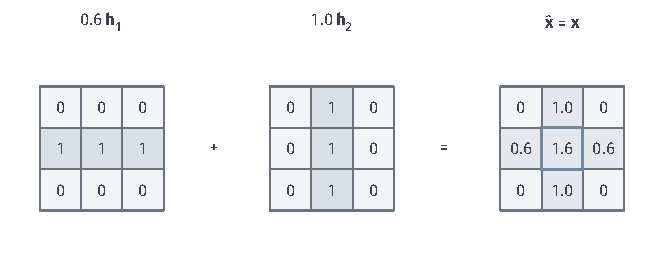
\includegraphics[width=112.000mm]{figures/04-classic-models/00-shared/tikz/dim-nmf-parts/figure.pdf}
  \caption{两个非负基的加性重构。左侧两幅$3\times3$栅格分别给出未加权的横条、竖条基，外侧系数为$0.6$与$1.0$；右侧为逐像素加权和，粗框中心格等于$0.6+1.0=1.6$。数值无量纲，本构造恰好精确重构，不表示NMF总能学出这样的部件或保证唯一分解。}
  \label{fig:dim-nmf-parts}
\end{figure}

观测类型决定怎样衡量重构误差。连续观测常用$\frac12\lVert\bm{X}-\bm{W}\bm{H}\rVert_F^2$，对应固定方差高斯残差的似然；非负计数可以使用广义KL散度，也称I散度：
\begin{equation}
  \mathcal{L}_{\mathrm{KL}}
  =\sum_{i,j}\left[
      \bm{X}_{i,j}\log\frac{\bm{X}_{i,j}}{(\bm{W}\bm{H})_{i,j}}
      -\bm{X}_{i,j}+(\bm{W}\bm{H})_{i,j}\right].
  \label{eq:dim-nmf-kl}
\end{equation}
计算采用$0\log(0/u)=0$；观测$\bm{X}_{i,j}>0$而重构为零时，损失为无穷大。条件独立Poisson计数的负对数似然与上式只差数据常数；存在过度离散时，则需要调整观测模型。

NMF的分解具有尺度和排列自由度。对正对角矩阵$\bm{D}$，$\bm{W}\bm{H}=(\bm{W}\bm{D})(\bm{D}^{-1}\bm{H})$，同时交换基与对应系数也保持重构。稀疏、平滑和归一化可以减少部分歧义，唯一性仍需相应识别条件。

\subsubsection{参数学习}
\label{sec:dim-nmf-learning}

基与系数的联合优化非凸，固定一侧后，平方误差子问题则是非负约束凸问题。Lee与Seung的乘法更新用非负比率维持可行性；下面的乘除均逐元素计算，两侧按顺序更新\scite{lee2001nmf}
\begin{equation}
  \begin{aligned}
    \bm{W}&\leftarrow\bm{W}\odot
       \frac{\bm{X}\bm{H}^{\top}}
        {\bm{W}\bm{H}\bm{H}^{\top}},\\
    \bm{H}&\leftarrow\bm{H}\odot
       \frac{\bm{W}^{\top}\bm{X}}
        {\bm{W}^{\top}\bm{W}\bm{H}}.
  \end{aligned}
  \label{eq:dim-nmf-mu}
\end{equation}
实现乘法更新时需要处理零分母；零元素可能被锁定，还应检查约束梯度残差，并比较多次初始化结果。

其他求解方式可以更直接地检查约束残差。投影梯度用$\max(0,\cdot)$返回非负区域，交替非负最小二乘更充分地求各子问题；HALS和坐标下降逐个更新基或系数，可以利用稀疏结构。达到给定精度的速度取决于损失、稀疏性和初始化，目标单调性只说明下降性质\scite{lin2007nmf}

固定$\bm{H}$后，新样本通过非负最小二乘或相应KL目标编码。平方误差下求$\min_{\bm{w}\geq0}\lVert\bm{x}-\bm{H}^{\top}\bm{w}\rVert_2^2$，需要求系数，而非复用一个线性投影。稠密平方误差更新的主要乘法约需$O(ndk)$，训练总成本还取决于迭代次数。

\subsubsection{理论分析}

\paragraph{表达能力}
固定共享基$\bm H$后，NMF能精确重构的观测集合是
\[
 \mathcal C_H=\{\bm H^\top\bm w:\bm w\in\mathbb R_+^k\}.
\]
它是由$k$个非负基生成的锥：每个系数表示添加多少相应成分。若真实观测以概率一属于$\mathcal C_H$，非负编码便能精确重构；一般观测的最佳平方误差则是到这个锥的距离平方。锥位于至多$k$维的线性空间内，所以线性低秩逼近误差仍是下限，非负限制还可能增加误差。例如只提供横条和竖条两个基，就能生成图\ref{fig:dim-nmf-parts}中的加性图案。若要求中心像素为零而其他条形像素为正，这两个基却不能生成该图案，因为中心值等于两个非负系数之和。

精确重构也不一定识别唯一成分。若字典同时含二维坐标向量$\bm e_1,\bm e_2$及其和$\bm e_1+\bm e_2$，观测$(1,1)^\top$既可用前两个基各一次，也可只用第三个基一次。这是系数歧义，尚未计入学习共享基本身的自由度。额外稀疏、分离或已知成分约束是否能消除歧义，要在这些约束下单独判断；非负性本身不保证基对应真实物质或语义部件。


\paragraph{收敛性}
平方误差NMF的最小值可以达到。为看清尺度问题，把每个非零基向量归一化为$\ell_1$范数一，并将缩放吸收到其系数中；零基可替换为任意归一化非负向量且令系数为零。在一个不劣于零重构的目标水平集内，重构矩阵有界；非负性使每条记录的系数和等于其重构向量的$\ell_1$范数，因而系数也有界。基与系数于是可限制在闭有界集合中，连续目标取得最小值。

正初始化且乘法更新始终有定义时，辅助函数论证给出目标不增加；目标有零下界，所以目标值收敛。这个结论没有给出统一收敛速度，也未单独保证参数收敛到驻点。固定一侧的非负最小二乘是凸子问题，可以用投影梯度控制子问题误差；交替更新两侧仍是非凸求解，不能沿用单个凸子问题的全局保证。

\paragraph{泛化性}
NMF为每个训练样本拟合一组系数，但可复用的是共享基。评价新记录时，要冻结基，再按同一约束求系数；这样才得到从经验重构到总体重构的同一个损失。以下给出带幅度限制的平方误差版本，也供稀疏字典使用。

\begin{theorem}[NMF在有界基与系数下的期望重构风险界]
 \label{thm:dim-dictionary-risk}
 设$\lVert\bm X\rVert_2\leq r$几乎处处，训练样本独立同分布。
 字典$\bm B\in\mathbb R^{d\times q}$的每列范数至多为$1$；
 系数集合$\mathcal A\subseteq\{\bm a:\lVert\bm a\rVert_1\leq c\}$在抽样前固定、为紧集并包含零。
 取连续惩罚$g\geq0$且$g(\bm0)=0$，定义
 \[
 \ell_{\bm B}(\bm x)=\min_{\bm a\in\mathcal A}
   \{\tfrac12\lVert\bm x-\bm B\bm a\rVert_2^2+g(\bm a)\},
 \qquad R(\bm B)=\mathbb E_P\ell_{\bm B}(\bm X).
 \]
 字典可另有抽样前固定的非负或结构约束。设$\widehat{\bm B}$的经验风险距该候选族全局最优的差为$e_n$，则
 \begin{equation}
  \mathbb E_{D_n}R(\widehat{\bm B})
  \leq\inf_{\bm B}R(\bm B)
   +\frac{4c(r+c)}n
   +r^2\sqrt{\frac{dq\log(1+2n)+\log2}{2n}}
   +\mathbb E_{D_n}e_n.
  \label{eq:dim-dictionary-risk}
 \end{equation}
\end{theorem}
\begin{proof}
零系数给出$0\leq\ell_{\bm B}\leq r^2/2$。若两组字典的每列距离至多为$\epsilon$，相同系数产生的重构距离至多为$c\epsilon$，残差范数至多为$r+c$，所以最小化后的损失差至多为$c(r+c)\epsilon$。列范数球的乘积有至多$(1+2/\epsilon)^{dq}$个覆盖点；有额外固定约束时，可在该候选集内选覆盖点并保持这一上界。引理\ref{thm:clustering-cover-risk}取$M=r^2/2$、$L=c(r+c)$与$\epsilon=1/n$，得到结论。
\end{proof}

对NMF，可规范化共享基$\bm H^\top$的列，并在训练和新点编码中同时要求系数非负、$\ell_1$范数至多为$c$；取$q=k$、$g=0$，式\eqref{eq:dim-dictionary-risk}便是该受约束NMF的总体重构界。系数幅度限制是本结论的条件，并非所有无约束NMF都自动满足。非凸交替求解及不精确编码进入$e_n$；训练残差下降并不消除这项误差。广义KL版本在重构趋零时损失可无界，需另设正下界或采用相应尾部条件。

\subsubsection{优化解释能力}

\paragraph{限制单条记录使用的成分数}
非负性只要求各成分相加，并没有要求一条记录只用少量成分。若解释希望每篇文档集中于几个主题，或每条光谱主要由少数材料组成，就可以在非负系数上再施加稀疏约束。约束前需要规范化基的尺度，否则放大基、缩小系数就能降低系数惩罚，而不改变重构。稀疏约束缩小了允许的组合，可能增加重构误差，也改变系数的求解。

\paragraph{限定成分的共同使用方式}
有些成分需要共同出现，只限制活跃成分数还不能表达这种关系。例如，可以把同一来源的几个谱峰作为一组，按组比较是否使用这些成分。分组约束把这种取舍写入系数学习，协调各组的使用，而不必要求组内每个系数都非零。分组是否符合实际组成仍要验证，更新也需处理相应的联合约束。

\subsubsection{小结}
\label{sec:dim-nmf-summary}

NMF让非负基与非负系数组成观测，适合需要加性成分的解释。成分数与损失决定怎样比较重构，非凸求解和表示歧义则影响学得的分解。把中心化后的负值平移成非负会改变加性的基准，需要由测量或任务含义支持。

少量成分参与与成分共同出现是不同要求，分别可以通过稀疏或分组约束调整系数学习。解释需要这些结构时，应同时比较重构损失、成分含义与新点编码成本。

文档主题还可以由概率模型描述。Ding、Li与Peng说明，在相应归一化和计数似然约定下，广义KL形式的NMF与概率隐语义索引的目标存在联系，更新算法仍不同\scite{ding2008nmf-plsi}。潜在狄利克雷分配进一步为主题比例设置先验\scite{blei2003}；它改变了生成假设和推断任务，不能仅凭矩阵形式相似就当作NMF求解器。

\subsection{稀疏编码与字典学习}
\label{sec:dim-sparse-coding}

一个图像块可能只含几条边缘，不同图像块中的边缘位置与方向却各不相同。若只保留少数PCA方向，这些变化都要由同一组小基底组合；若希望为许多边缘形态都准备候选基，又不想让每个图像块使用全部候选，就可以允许字典较大、单个样本的活跃系数较少。\term{稀疏编码}（sparse coding）在固定字典中求这些系数，\term{字典学习}（dictionary learning）进一步从数据学习共享的基。稀疏性约束每次使用多少基，非负性则约束组合符号，两种要求可以分别采用，也可以同时采用。

Olshausen与Field在1996年研究自然图像的统计规律是否能解释初级视觉皮层响应的局部性、方向选择性与空间频率选择性。他们用稀疏线性编码学习具有这些性质的基，并与小波表示比较\scite{olshausen1996}这给视觉神经科学和信号表示建立了联系；感受野外观相似的证据，仍不足以确定生物学习过程与该算法相同。

\subsubsection{模型结构}
\label{sec:dim-sparse-coding-structure}

把共享基作为$\bm{D}\in\mathbb{R}^{d\times p}$的列，称$\bm{d}_j$为字典原子，$p$为原子数。允许$p>d$时，字典称为过完备。样本由$\bm{x}_i\approx\bm{D}\bm{\alpha}_i$重构，$\bm{\alpha}_i\in\mathbb{R}^{p}$只激活少数坐标。取$\lambda>0$控制稀疏惩罚的强度，通过误差与惩罚的加权和选择字典和系数：
\begin{equation}
  \begin{aligned}
  \min_{\bm{D},\{\bm{\alpha}_i\}}\quad&
   \sum_{i=1}^{n}\left[
      \tfrac12\lVert\bm{x}_i-\bm{D}\bm{\alpha}_i\rVert_2^2
      +\lambda\lVert\bm{\alpha}_i\rVert_1\right],\\
  \text{约束}\quad&\lVert\bm{d}_j\rVert_2\leq1
                 \quad(j=1,\ldots,p).
  \end{aligned}
  \label{eq:dim-dictionary-objective}
\end{equation}
若字典无限放大、系数相应缩小，重构不变而$\ell_1$惩罚降低；列范数约束排除了这种尺度退化。此模型允许正负系数和非正交基，表示长度甚至可以超过原维数，与NMF的非负及PCA的正交约束不同。

\subsubsection{参数学习}
\label{sec:dim-sparse-coding-learning}

$\lambda>0$时的惩罚解通常会收缩系数。即使$\bm x=\bm D\bm\alpha\ne\bm0$能精确重构，把系数缩为$(1-t)\bm\alpha$只增加二次量级的残差，却减少一次量级的稀疏惩罚；足够小的$t>0$会降低目标。因此不能把存在精确稀疏表示，直接写成Lasso型编码一定零残差。

给定字典后，每个样本独立求Lasso型系数，可用坐标下降、LARS或近端梯度。对一个样本，取$L\geq\lVert\bm{D}^{\top}\bm{D}\rVert_2$且$L>0$，ISTA把重构误差的梯度步与稀疏惩罚结合：
\begin{equation}
  \bm{\alpha}^{(t+1)}
  =\mathcal{S}_{\lambda/L}\left(
      \bm{\alpha}^{(t)}
      +L^{-1}\bm{D}^{\top}
          (\bm{x}-\bm{D}\bm{\alpha}^{(t)})\right).
  \label{eq:dim-ista}
\end{equation}
该更新先沿重构误差的负梯度移动，再作$\ell_1$惩罚的软阈值近端映射。FISTA增加外推，在固定字典的凸子问题条件下改善目标值收敛率；字典与系数联合学习仍需单独分析\scite{beck2009fista}

给定编码，记$\bm{A}=[\bm{\alpha}_1,\ldots,\bm{\alpha}_n]\in\mathbb{R}^{p\times n}$，字典步最小化$\frac12\lVert\bm{X}^{\top}-\bm{D}\bm{A}\rVert_F^2$并满足列范数约束。MOD用无约束解$\bm{X}^{\top}\bm{A}^{\dagger}$更新方向，常见实现再归一化各列。各字典列共同影响重构残差，无约束解后逐列归一化一般不能得到列范数约束下的精确解。需要严格下降时，应采用适当的约束求解或验证更新。

K-SVD通常采用$\lVert\bm{\alpha}_i\rVert_0\leq s$的活跃原子数约束。更新一个原子时，先去掉其他原子的重构，只保留使用该原子的样本，再用残差的秩一SVD同时更新原子与活跃系数。该求解配合的是非零项数约束，与式\eqref{eq:dim-dictionary-objective}的$\ell_1$目标不同\scite{aharon2006ksvd}

\subsubsection{理论分析}

\paragraph{表达能力}
若硬性限制每个样本至多使用$s$个原子，候选重构集合为各支持集张成的子空间之并：
\begin{equation}
 \mathcal C_{D,s}
 =\bigcup_{|S|\leq s}\operatorname{span}\{\bm d_j:j\in S\}.
 \label{eq:dim-sparse-coding-representation}
\end{equation}
真实观测落在这一集合中时，存在精确稀疏重构；否则最佳平方残差就是到该集合的距离平方。更换支持集可以表达不同边缘形态，不必把全部样本塞进同一个$s$维子空间。不过有限字典、$s=1$只能给出有限条直线，无法精确表示连续变化的整条圆周。这里的硬支持限制对应K-SVD等设定，式\eqref{eq:dim-dictionary-objective}的$\ell_1$惩罚本身并未指定固定的非零项数。

重构准确与编码唯一也有区别。若字典任意至多$2s$列都线性无关，则两个$s$稀疏编码不可能生成同一个非零观测：相减会产生一个至多$2s$稀疏的零空间向量，与该条件矛盾。重复原子或高度相关原子则可能使编码不唯一或对噪声敏感。



\paragraph{收敛性}
\begin{theorem}[固定字典下稀疏编码解的存在性与ISTA、FISTA收敛速度]
固定字典且$\lambda>0$时，单样本目标$F(\bm\alpha)=\tfrac12\lVert\bm x-\bm D\bm\alpha\rVert_2^2+\lambda\lVert\bm\alpha\rVert_1$为连续凸函数，并在系数趋于无穷时趋于无穷，故最小值存在。字典列不独立时，最优系数未必唯一。取$L\geq\lVert\bm D^\top\bm D\rVert_2$、$L>0$，ISTA和标准FISTA对任一最优系数$\bm\alpha_\star$分别满足
\[
 \begin{aligned}
 F(\bm\alpha^{(t)})-F(\bm\alpha_\star)
 &\leq\frac{L\lVert\bm\alpha^{(0)}-\bm\alpha_\star\rVert_2^2}{2t},\\
 F(\bm\alpha_{\mathrm{FISTA}}^{(t)})-F(\bm\alpha_\star)
 &\leq\frac{2L\lVert\bm\alpha^{(0)}-\bm\alpha_\star\rVert_2^2}{(t+1)^2}.
 \end{aligned}
\]
\end{theorem}

后一方法以外推把目标差的$O(1/t)$改善为$O(1/t^2)$\scite{beck2009fista}。联合学习时，字典列范数约束与正的$\ell_1$惩罚分别控制字典、系数的大小，最小值仍可达到，但联合目标非凸。交替步骤即使逐次下降，也不能直接继承固定字典的速度与全局最优结论。

\paragraph{泛化性}
稀疏编码的新点风险可以使用与训练相同的惩罚重构损失：
$R_\lambda(\bm D)=\mathbb E_P\min_{\bm\alpha}
\{\tfrac12\lVert\bm X-\bm D\bm\alpha\rVert_2^2
+\lambda\lVert\bm\alpha\rVert_1\}$。
\begin{theorem}[稀疏编码在有界输入与字典下的期望重构风险界]
 \label{thm:dim-sparse-coding-risk}
设$D_n$独立同分布于$P$，假设$\lVert\bm X\rVert_2\leq r$、$\lambda>0$且字典列范数至多为$1$。
零编码的损失至多为$r^2/2$，所以每个最优编码都满足
$\lVert\bm\alpha\rVert_1\leq c_\lambda:=r^2/(2\lambda)$。
将系数限制到这一紧球不改变最优编码，定理\ref{thm:dim-dictionary-risk}因而给出
\begin{equation}
 \begin{aligned}
 \mathbb E_{D_n}R_\lambda(\widehat{\bm D})
 &\leq\inf_{\bm D}R_\lambda(\bm D)
       +\frac{4c_\lambda(r+c_\lambda)}n\\
 &\quad+r^2\sqrt{\frac{dp\log(1+2n)+\log2}{2n}}
       +\mathbb E_{D_n}e_n.
 \end{aligned}
 \label{eq:dim-sparse-coding-risk}
\end{equation}
\end{theorem}

$e_n$衡量联合字典学习的经验误差，内层编码未精确求解也须纳入求解评价。这里比较的是惩罚重构风险，不能将右侧最佳值改成无惩罚重构风险。减小$\lambda$允许更大的系数，也使本界的幅度常数增大；$\ell_0$约束的K-SVD还需另控制系数幅度。预先固定的非负、分组或卷积结构可进入候选集，但数据选择结构时须另计选择复杂度。

\subsubsection{优化解释能力}

只要求系数稀疏，没有规定哪些原子应当一起使用。若若干原子描述同一来源的不同部分，可以用分组约束协调它们的激活。它改变的是允许的活跃组合，与标签监督或位置共享各自回答的问题不同；额外结构应由信号组成支持，并配套相应的编码方法。

\subsubsection{优化计算能力}

\paragraph{降低计算与存储成本}
反复交替求全部样本的编码与字典，会重复读取大规模训练数据。在线字典学习按小批样本更新，积累编码二阶统计量及观测交叉统计量以近似求字典，减少反复扫描全数据的开销。总成本还取决于原子数、每个稀疏子问题的精度和更新次数，一次遍历不能确定达到指定精度的完整成本\scite{mairal2009online}。

\paragraph{减少重复位置的原子存储}
同一个局部边缘反复出现在不同位置时，为每个位置分别保存原子会重复记录相同模式。卷积稀疏编码改为在位置之间共享滤波器，由系数指出出现位置；它减少了重复基，却引入平移共享的假设及卷积编码的计算。

\subsubsection{支持标签监督的字典学习场景}

重构得好未必保留预测信息。例如，图像中的背景占据较大能量，区分类别的局部细节却可能很小，只拟合重构时，字典可能优先分配原子给背景。让标签参与字典学习，可以用预测损失与重构损失共同选择原子；代价是增加监督目标及其权重，也要将标签参与的字典训练放入验证流程。

\subsubsection{小结}
\label{sec:dim-sparse-coding-summary}

稀疏编码用少量活跃原子组合信号，字典学习再调整这些共享原子，适合去噪、修复与局部模式表示。过完备字典可以准备更多模式，系数也可能比输入更长；稀疏表示不等于坐标维数更低。新样本仍需推断系数，训练与使用都要预留优化预算。

预测任务可让标签参与原子选择，重复局部模式可采用位置共享，成分共现可采用结构约束。这些调整分别改变要保留的信息、基的复用方式与允许的组合，也改变求解成本。应先确认缺口位于哪一步，再选择约束，而不是仅凭系数更稀疏判断表示更合适。

\subsection{随机投影（Random Projection）}
\label{sec:dim-rp}

前述投影和字典都先从数据学习。流式输入的维数很高时，保存协方差或反复拟合方向可能超过预算；如果后续任务主要使用点间欧氏距离，就可以改为先固定一个较小的映射。\term{随机投影}（random projection）按指定分布抽取矩阵，再统一变换全部样本，不需要先找出方差最大的方向。Johnson--Lindenstrauss引理说明，输出维数足够时，针对抽取映射前固定的有限点集，所有点对距离都能以较高概率近似保留\scite{johnson1984jl}它用随机保距换取省去方向拟合的计算，但不直接提供PCA式的最小重构误差。

实现这种映射还要考虑生成和计算成本。Achlioptas于2003年构造离散随机矩阵，让投影由属性的加减、聚合和统一缩放实现\scite{achlioptas2003}其变化在于算术操作，有限点集上的几何保证仍不依赖先拟合数据。

\subsubsection{模型结构}
\label{sec:dim-rp-structure}

用$\bm{\Pi}\in\mathbb{R}^{k\times d}$编码$\bm{z}=\bm{\Pi}\bm{x}$。独立高斯元素$\bm{\Pi}_{i,j}\sim\mathcal{N}(0,1/k)$给出最直接的构造：对固定$\bm{x}$，平方范数的平均值为
\[
  \mathbb{E}_{\bm{\Pi}}\lVert\bm{\Pi}\bm{x}\rVert_2^2
  =\lVert\bm{x}\rVert_2^2.
\]
该期望只说明平均保范数。一次采样要同时服务整批样本，还需控制偏离均值的尾概率，再让各点对的误差同时受限。

稀疏矩阵进一步减少乘法和存储。Achlioptas的元素以$1/6$概率取$\sqrt{3/k}$、以$1/6$概率取$-\sqrt{3/k}$，其余取零，也可建立集中界。Li、Hastie与Church研究更稀疏的构造时，还需考虑输入分量的集中程度；二阶矩相同并不足以支持任意稀疏率下的同一误差界\scite{li2006sparserp}

快速Johnson--Lindenstrauss变换用随机符号、Hadamard变换及后续抽样或稀疏映射组织计算。结构化变换部分约为$O(d\log d)$，总成本还包括输出维数和精度相关项。与直接存储$kd$个高斯元素相比，它对内存、算术和输入尺寸有不同要求\scite{ailon2009fjlt}

\subsubsection{参数学习}
\label{sec:dim-rp-learning}

随机投影直接生成映射，需要选择的是$k$、矩阵分布和稀疏程度。训练与新样本使用相同矩阵，稠密编码每样本约需$O(kd)$次运算。分布式环境若用共同种子复现映射，还要固定伪随机数实现和矩阵元素的生成顺序。

输出维数决定误差、点数和失败概率之间的取舍。下面的充分条件往往保守，给出的$k$若已超过$d$，就没有实际压缩收益。可以在训练或验证数据上测量距离失真，比较较小维数，或先随机压缩到中等维数再做PCA、最近邻搜索；下游结果则按任务另行评价。

对映射抽取前固定的有限点集，高斯随机投影给出同时保留平方距离的充分维数条件，可用来设置候选$k$（参见\BookTheoremRef{thm:probability-johnson-lindenstrauss}{卷2《数学准备：概率、因果与决策》第1章“随机变量”第1.4.2节“候选族累计量的统一偏差控制”}）。观察映射后，从这批固定点中选择要比较的点对，仍被同时保距事件覆盖；观察映射后再构造点集之外的新查询，则超出这里的固定点集保证。

若所有观测落在一个预定$m$维线性子空间，$k\geq m$的高斯投影以概率一在该子空间上单射：把投影限制到一组子空间基，得到一个以概率一满列秩的$k\times m$高斯矩阵。这个结论只保证所选子空间上的单射，距离失真还需要另行控制。

要用一次采样同时服务全部点对，需要让维数足以控制整批失败概率。给定点数、相对误差和失败概率后，可使用以下充分条件。

对$n\geq2$个预先固定的点，取$0<\varepsilon,\delta<1$。
上述定理给出充分条件
\[
  k\geq\frac{8}{\varepsilon^2}\log\frac{n(n-1)}{\delta},
\]
使同一高斯投影以至少$1-\delta$的概率同时把全部点对的平方距离保持在原值的
$1\pm\varepsilon$倍内。这里$\delta$控制整批点对的失败概率，不是每一对单独的失败概率。

在相应参数区间，JL的$\varepsilon^{-2}\log n$维数尺度有匹配下界\scite{larsen2017jl}例如要求失败概率至多$1/n$时，可取$k\geq24\log n/\varepsilon^2$。具体集中界决定常数；主要尺度随点数对数增长，上界本身不直接依赖$d$。

\subsubsection{理论分析}
\label{sec:dim-rp-theory}

\paragraph{表达能力}
随机投影能以少量坐标近似保留预先固定点集的欧氏关系，前述JL条件给出全部点对的相对失真。这个目标没有要求重构原向量。$k<d$时，$\bm\Pi$有非零零空间；对任一$\bm v\ne0$且$\bm\Pi\bm v=\bm0$，$\bm x$与$\bm x+\bm v$的编码相同。因此它不可能在整个$\mathbb R^d$上既压缩又精确保距、可逆。

限制数据支持后，结论可以不同。若所有观测落在一个预定线性子空间，且投影在该子空间上单射，已知该子空间时便可反求坐标；距离失真仍需另行控制。对有限点集，$k$甚至可以小于点集的仿射维数而近似保距；这正是有限集近似与整个支持上的精确表示之间的区别。

\paragraph{收敛性}
映射按预设分布采样，所以没有训练目标的迭代求解。稠密高斯矩阵生成和存储为$O(kd)$规模，每个输入也约需$O(kd)$运算。增大$k$是在保距精度和计算成本之间选择，而非提高训练收敛速度。

\paragraph{泛化性}
JL界同时控制预先固定的有限点集；新样本风险还可以按新点对的分布单独计算。

\begin{theorem}[高斯随机投影的期望相对距离误差]
 \label{thm:dim-rp-risk}
取整数$k\geq1$及$0<\delta<1$。设$\bm A$的元素独立服从$\mathcal N(0,1/k)$，且$\bm A$独立于$\bm X,\bm X'\overset{\mathrm{iid}}\sim P$。用相对平方距离失真评价固定映射：
\[
 R(\bm A)=\mathbb E_{\bm X,\bm X'}
 \left[\left(\frac{\lVert\bm A(\bm X-\bm X')\rVert_2^2}
                    {\lVert\bm X-\bm X'\rVert_2^2}-1\right)^2
              \mathbf1\{\bm X\ne\bm X'\}\right],
\]
重合点的被积项约定为零。对每个非零固定向量，距离比服从$\chi_k^2/k$，其均值为$1$、方差为$2/k$；先对映射、再对新点积分，得到
\begin{equation}
 \mathbb E_{\bm A}R(\bm A)=\frac2kP(\bm X\ne\bm X')\leq\frac2k,
 \qquad
 P_{\bm A}\{R(\bm A)\leq2/(k\delta)\}\geq1-\delta.
 \label{eq:dim-rp-risk}
\end{equation}
\end{theorem}

第二个结论由Markov不等式得到。若$\mathbb E\lVert\bm X-\bm X'\rVert_2^4<\infty$，未归一化的平方距离误差也满足
\[
 \mathbb E_{\bm A,\bm X,\bm X'}
 \left(\lVert\bm A(\bm X-\bm X')\rVert_2^2
              -\lVert\bm X-\bm X'\rVert_2^2\right)^2
 =\frac2k\mathbb E\lVert\bm X-\bm X'\rVert_2^4.
\]
这里没有经验风险最小化步骤，误差由随机映射的分布直接控制，样本数$n$不进入这一平均新点对风险。$k<d$时映射仍有非零核空间，因而不能同时保留所有向量。观察映射后专门选择落入核空间的查询违反独立性条件；流式新点若按固定$P$独立到来，则满足上述风险设定。

\subsubsection{小结}
\label{sec:dim-rp-summary}

随机投影可以用于流式或超高维预处理，无需先拟合输入分布。它以给定度量下的点集几何为目标；预测信息是否保留、所需维数及矩阵计算预算仍需按用途评价。

\subsection{核主成分分析（Kernel PCA）}
\label{sec:dim-kpca}

PCA只能在原坐标中选择直的子空间。以二维构造数据$(x,x^2)$为例，所有点由一个标量控制，却沿抛物线变化；用一条直线重构时，曲线偏离直线的部分会留下误差。对这个已知构造，映射$\bm\phi(u,v)=(u,v-u^2)$把点变成$(x,0)$，一个直线方向就足以表示它们。这个例子说明，先改变特征表示，再做线性降维，可以表达原坐标中弯曲的变化。

\term{核主成分分析}（kernel principal component analysis, Kernel PCA）在非线性特征空间中选择主方向，用核函数计算所需的内积，省去显式列出特征的步骤。Schölkopf、Smola与Müller于1998年提出了这一核特征值方法\scite{dimScholkopf1998}与前述已知抛物线的构造不同，实际数据需要选择并检验合适的核。核PCA优化的是核特征空间的方差与重构，原坐标中的重构还需要求逆映射，不能直接由特征空间误差代替。

\subsubsection{模型结构}

这里需要的特征由第\ref{sec:classic-overview-kernel-validity}节的正定核$K$定义，记Hilbert空间为$\mathcal{H}$、映射为$\bm{\phi}$。训练核矩阵及中心化矩阵$\bm{H}$沿用第\ref{sec:classic-overview-kernel-matrix}节。核PCA以保留特征方差为目标，核SVM的间隔目标则用于分类。

方差要相对于训练特征均值计算，因此取
\[
  \bar{\bm{\phi}}=\frac1n\sum_i\bm{\phi}(\bm{x}_i),
  \qquad
  \bm{\phi}_{\mathrm{c}}(\bm{x})=\bm{\phi}(\bm{x})-\bar{\bm{\phi}}.
\]
方向$\bm{v}\in\mathcal{H}$上的经验协方差运算为
\begin{equation}
  \label{eq:dim-kpca-covariance}
  \widehat{\mathcal{C}}\bm{v}
  =\frac1n\sum_i
    \bm{\phi}_{\mathrm{c}}(\bm{x}_i)
    \langle\bm{\phi}_{\mathrm{c}}(\bm{x}_i),\bm{v}\rangle_{\mathcal{H}}.
\end{equation}
若$\widehat{\mathcal{C}}\bm{v}=\lambda^{\mathrm{C}}\bm{v}$且$\lambda^{\mathrm{C}}>0$，右侧的有限和说明$\bm{v}$落在中心化训练特征张成的空间。正特征值方向因而可以用训练特征展开；零特征值方向没有这一约束。

将方向写为$\bm{v}_\ell=\sum_i(\bm{\alpha}_\ell)_i\bm{\phi}_{\mathrm{c}}(\bm{x}_i)$，并令$\bm{K}_{\mathrm{c}}=\bm{H}\bm{K}\bm{H}$。代入协方差方程，核矩阵特征值满足$\lambda_\ell^{\mathrm{K}}=n\lambda_\ell^{\mathrm{C}}$，把特征空间的谱计算转成样本矩阵计算。

\subsubsection{参数学习}

核矩阵的单位特征向量需要缩放，才能成为特征空间单位方向的展开系数。令$\bm{u}_\ell$为中心化核矩阵的欧氏单位特征向量，归一化关系为
\begin{equation}
  \label{eq:dim-kpca-normalization}
  \begin{aligned}
    \bm{K}_{\mathrm{c}}\bm{u}_\ell
      &=\lambda_\ell^{\mathrm{K}}\bm{u}_\ell,
      \qquad\lVert\bm{u}_\ell\rVert_2=1,\\
    \bm{\alpha}_\ell
      &=\frac{\bm{u}_\ell}{\sqrt{\lambda_\ell^{\mathrm{K}}}},\\
    \lVert\bm{v}_\ell\rVert_{\mathcal{H}}^2
      &=\bm{\alpha}_\ell^{\top}\bm{K}_{\mathrm{c}}\bm{\alpha}_\ell=1.
  \end{aligned}
\end{equation}
将各训练点投到方向$\bm{v}_\ell$，得到表示矩阵的一列：
\begin{equation}
  \label{eq:dim-kpca-training}
  \bm{Z}_{:,\ell}
  =\bm{K}_{\mathrm{c}}\bm{\alpha}_\ell
  =\sqrt{\lambda_\ell^{\mathrm{K}}}\,\bm{u}_\ell
  =\lambda_\ell^{\mathrm{K}}\bm{\alpha}_\ell.
\end{equation}
$\bm{u}_\ell$在欧氏范数下归一化，$\bm{\alpha}_\ell$则使特征空间方向范数为一。因此训练坐标是$\sqrt{\lambda_\ell^{\mathrm{K}}}\bm{u}_\ell$，展开系数乘上的尺度要按上式计算，不能改为$\sqrt{\lambda_\ell^{\mathrm{K}}}\bm{\alpha}_\ell$。

选择核相当于先决定观察输入的哪些变化。图\ref{fig:dim-kernel-radial}用$\phi(\bm{x})=\lVert\bm{x}\rVert_2^2$只记录半径平方，$K(\bm{x},\bm{y})=\phi(\bm{x})\phi(\bm{y})$由此为正半定核。两圆样本数相同，均值为$(1+4)/2=2.5$，中心化坐标为$-1.5$和$1.5$。径向差异得以保留，角度在特征映射中已丢失，后续PCA无法恢复。

\begin{figure*}[htbp]
  \centering
  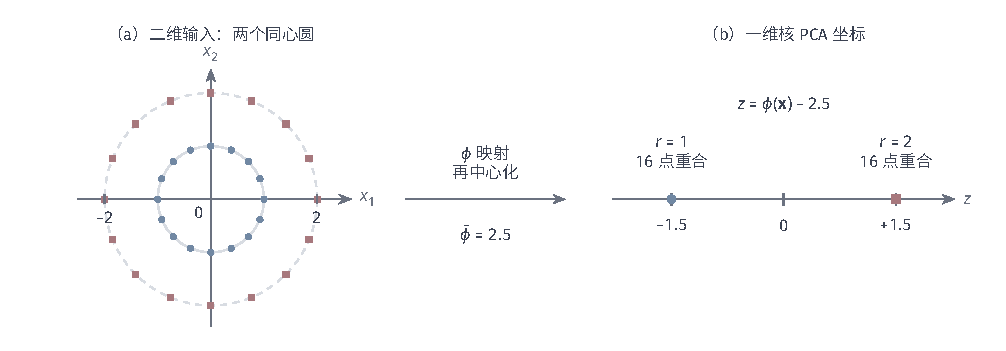
\includegraphics[width=169.000mm]{figures/04-classic-models/00-shared/tikz/dim-kernel-radial/figure.pdf}
  \caption{由核选择保留量的构造例子。左图在半径为$1,2$的圆上各取16个等角度样本，圆点与方点区分两圈。所示特制核对应标量特征$\phi(\bm{x})=\lVert\bm{x}\rVert_2^2$，中心化核矩阵秩为1；选择图示主轴方向，核PCA坐标为$\pm1.5$。右侧每个标记表示16点重合，坐标无量纲。此结果依赖所选核，不能推广为任意高斯核或多项式核的输出。}
  \label{fig:dim-kernel-radial}
\end{figure*}

新样本必须沿用训练特征均值，才能与训练表示处于同一坐标系。令$\bm{k}(\bm{x})_i=K(\bm{x}_i,\bm{x})$，中心化及投影为
\begin{equation}
  \label{eq:dim-kpca-extension}
  \begin{aligned}
    \bm{k}_{\mathrm{c}}(\bm{x})
      ={}&\bm{k}(\bm{x})-\frac1n\bm{K}\bm{1}\\
         &-\frac1n\bm{1}\bm{1}^{\top}\bm{k}(\bm{x})
          +\frac1{n^2}\bm{1}\bm{1}^{\top}\bm{K}\bm{1},\\
    z_\ell(\bm{x})
      ={}&\bm{\alpha}_\ell^{\top}\bm{k}_{\mathrm{c}}(\bm{x}).
  \end{aligned}
\end{equation}
两个减项分别扣除与训练均值的内积，末项补回均值自内积。只减新核向量自身均值会漏掉这些量；加入新点重算均值，则是在改变原先的映射。

高斯核带宽过大时，各核值接近，中心化信号变弱；带宽过小时，核矩阵接近单位阵，主方向难以辨认。距离中位数可作初始尺度，再用任务验证选择。监督任务中的中心化和主方向均应在训练折拟合。

对当前训练点，误差相应为$n^{-1}\sum_{j>k}\lambda_j^{\mathrm K}$，所以保留中心化核矩阵的全部正谱能够精确重构训练特征，却未必提供低维压缩。

\subsubsection{理论分析}
\label{sec:dim-kpca-theory}

\paragraph{表达能力}
核PCA的候选重构仍是线性的，但线性子空间位于$\mathcal H$中。若$\mathcal H$可分且$\mathbb E K(\bm X,\bm X)<\infty$，总体特征协方差的有序特征值记为$\lambda_j^{\mathcal H}$，同样的正交分解给出最佳$k$维特征重构误差$\sum_{j>k}\lambda_j^{\mathcal H}$。只有中心化特征以概率一位于一个至多$k$维的子空间中，该误差才为零；输入由$k$个参数控制，并不自动满足这个核特征秩条件。

相对于原输入的非线性来自核映射，核也可能先丢掉信息。图\ref{fig:dim-kernel-radial}的径向核只保留半径，所有同半径点的编码相同，保留再多主方向也不能恢复角度。即使核映射可区分不同输入，有限维截断仍可能合并它们；特征重构点还不一定属于$\bm\phi(\mathbb R^d)$。因此特征误差小是否意味着原空间误差小，需要可逆性及逆映射稳定条件，不能仅由核技巧推出。

\paragraph{收敛性}

固定正定核后，经验方差目标可由谱分解全局求解，核矩阵近似及求谱精度决定数值误差。相同谱计算还连接点间距离：第\ref{sec:dim-mds}节定义经典MDS后，引理\ref{thm:dim-kpca-mds}将证明核诱导距离与中心化核PCA给出相同训练坐标。该联系针对特征距离，局部重构和图平滑则使用不同目标。

\paragraph{泛化性}
核PCA的新点公式定义了共享编码，期望风险则应按它实际优化的特征重构来评价。

\begin{theorem}[核PCA在有界核条件下的期望特征重构风险界]
 \label{thm:dim-kpca-risk}
设训练样本独立同分布于$P$，核在训练前固定、特征空间$\mathcal H$可分，且
$K(\bm x,\bm x)\leq\kappa^2$几乎处处。总体特征均值为$\bm m=\mathbb E\bm\phi(\bm X)$，训练特征均值为$\widehat{\bm m}$，所学秩$k$正交投影为$\widehat{\mathcal P}$。固定重构规则
$\widehat r_{\mathcal H}(\bm x)=\widehat{\bm m}
 +\widehat{\mathcal P}(\bm\phi(\bm x)-\widehat{\bm m})$后，定义
\[
 R_{\mathcal H,n}
 =\mathbb E_{\bm X\sim P}
   \lVert\bm\phi(\bm X)-\widehat r_{\mathcal H}(\bm X)\rVert_{\mathcal H}^2.
\]
新点独立于训练集。记$R_{\mathcal H,k}^\star$为以总体均值中心化后的最佳秩$k$投影风险，$e_n$为经验特征重构距全局最优的差。则
\begin{equation}
 \mathbb E_{D_n}R_{\mathcal H,n}
 \leq R_{\mathcal H,k}^\star
       +\frac{8\sqrt{k}\,\kappa^2}{\sqrt n}
       +\frac{4(2\sqrt{k}+1)\kappa^2}{n}
       +\mathbb E_{D_n}e_n.
 \label{eq:dim-kpca-risk}
\end{equation}
\end{theorem}

证明沿用定理\ref{thm:dim-pca-risk}：$\lVert\bm\phi(\bm X)-\bm m\rVert_{\mathcal H}\leq2\kappa$，有限矩阵的Frobenius范数换成协方差算子的Hilbert--Schmidt范数，即算子奇异值平方和的平方根；独立平均、均值校正和秩$k$投影的估计仍相同。取$r=2\kappa$便得到该界，特征空间不必有限维。核PCA的重构风险也有更细致的专门分析\scite{blanchard2007kpca}

经验协方差逼近总体协方差，使经验最佳投影的总体特征损失接近该族最佳值，这是风险转移所需的链路；谱隙只在进一步估计主子空间时需要。数据自适应核需另外控制核选择，不能将固定核界原样使用。式\eqref{eq:dim-kpca-risk}也不保证原输入重构：截断特征可能没有原像，原像算法还需独立误差分析。

\subsubsection{优化计算能力}

常用核的全矩阵构造约需$O(n^2d)$，存储为$O(n^2)$，稠密谱分解为$O(n^3)$。Nystr\"om近似使用代表列减少矩阵计算，随机Fourier特征则对合适的平移不变核构造有限特征后再做线性PCA。近似误差需要单独评价，适用核也各有条件。

两种近似处理的对象不同：代表列概括训练样本间的核关系，随机特征直接给输入一个有限维映射。前者仍依赖代表样本的覆盖，后者需要选择特征数；省去全核计算的同时，应检查近似后的谱方向与新点编码是否仍保留所需变化。

\subsubsection{小结}

核PCA先用核规定特征几何，再按方差选择该空间中的主方向。它能够让某些原空间非线性关系进入线性表示，却也可能在核映射时丢掉角度等信息；选核与选择保留维数因而回答不同问题。新样本须沿用训练中心化与核投影，原空间重构还需处理原像问题。

全核矩阵成为瓶颈时，代表列近似减少处理的样本方向，有限随机特征则对适用核先构造显式映射。两者节省不同计算，也引入不同近似。应同时比较核几何、近似精度和新点计算，不能把特征空间方差的改善直接解释为原输入重构或下游预测改善。

\subsection{模型对比与总结}
\label{sec:dim-linear-comparison}

同一组线性坐标可以为不同信息服务。PCA按输入方差选方向，适合保留主要变化；若大方差来自单侧噪声或任务无关因素，这一准则就没有理由优先保留所需信息。CCA让配对视图的共同变化决定方向，PLS与判别投影让响应或类别参与方向选择。它们改变的是选择方向的依据，输入、输出和验证数据也因此需要相应调整。

ICA进一步改变了要分离的统计关系。PCA的正交方向让得分不相关，但不相关仍可能包含非线性依赖；ICA用独立源假设及非高斯信息寻找解混方向。这里的任务是分离来源，标准方形ICA并不自动减少维数。源假设不成立时，换一个对比函数也不能保证得到真实来源。

重构方法的差别还在允许怎样组合基。PCA对全部样本使用一个正交子空间；稀疏PCA限制编码需要读取的变量，RPCA则把共享低秩信号与稀疏污染分开。NMF要求成分只作非负叠加，稀疏编码允许较大的字典和正负组合，再以稀疏约束控制每个样本的活跃原子。非负、稀疏、正交与异常污染分别约束不同对象，应按成分含义和污染方式组合，不能把一种约束当成其他要求的替代。

原空间的线性方向不够时，核PCA先改变观察输入的特征几何，再按该空间的方差选择方向。随机投影则省去数据方向的拟合，以固定随机矩阵压缩点间距离信息；它没有以最大方差或最小重构残差选择矩阵。表\ref{tab:dim-linear-comparison}把这些目标与新点编码并列，便于区分表示要保留什么，以及训练后怎样复用它。

\begin{table*}[htbp]
  \centering
  \small
  \begin{tabularx}{\linewidth}{@{}l>{\RaggedRight\arraybackslash}X>{\RaggedRight\arraybackslash}X>{\RaggedRight\arraybackslash}X@{}}
    \toprule
    方法 & 主要目标与约束 & 新样本的表示 & 典型边界\\
    \midrule
    PCA & 正交投影下保留方差 & 中心化后矩阵乘法 & 对尺度、异常值敏感\\
    CCA & 配对视图的相关性最大 & 两侧分别线性投影 & 需配对观测，易过拟合相关性\\
    ICA & 独立源的线性解混 & 白化及解混乘法 & 独立性、非高斯性与可识别性\\
    NMF & 非负基与非负系数重构 & 非负约束推断 & 非凸、通常不唯一\\
    稀疏编码 & 少量原子重构观测 & 稀疏优化 & 可为高维编码，需控制推断成本\\
    随机投影 & 随机矩阵近似保距 & 固定矩阵乘法 & 维数、误差与失败概率的权衡\\
    核PCA & 特征空间方差 & 训练中心化核投影 & 核几何、样本展开与原空间重构\\
    \bottomrule
  \end{tabularx}
  \caption{线性投影与线性组合方法的比较。目标成立均依赖各小节的具体条件；“新样本可编码”不等于编码具有统计泛化保证。}
  \label{tab:dim-linear-comparison}
\end{table*}

求解方式进一步决定预算。谱分解类方法主要处理协方差或数据矩阵，迭代拟合还需计入稀疏结构、停止精度与总轮数，固定映射则需计入生成和使用矩阵的成本。基可以追溯原始特征，是否对应可解释概念仍要由数据和任务验证。

选择线性组合时，先确定要保留的信息和新样本的编码方式。若还需解释各特征的测量误差，可转向第\ref{sec:dim-probabilistic}节的生成模型；只有对象差异时，下一节将讨论如何从距离安排坐标。原空间线性基不足以描述弯曲结构时，还需要改变特征或关系。

\section{基于距离的降维}
\label{sec:dim-distance}

对象之间的差异有时比原始坐标更容易取得，例如相似性评分或编辑距离。此时需要根据差异安排位置，而非直接投影特征。多维缩放提供了这种坐标恢复；下一节还会把差异限制到局部邻域，用来研究弯曲几何。

\subsection{多维缩放（MDS）}
\label{sec:dim-mds}

有时我们只有对象之间的差异，没有每个对象的向量坐标。例如，受试者可以评价两种气味有多相似，却不一定能为每种气味给出同一组数值属性；PCA因而缺少可以投影的坐标矩阵。\term{多维缩放}（multidimensional scaling, MDS）从点对差异反求低维位置，让这些位置的几何关系尽量符合输入。Young与Householder于1938年研究距离对坐标的代数约束，为坐标恢复建立了几何依据\scite{dimYoung1938}差异不一定能精确表示为指定维数中的欧氏距离，因此目标还需要规定允许怎样的失真。

Torgerson在1952年系统提出经典MDS时，还要处理心理距离怎样测量。刺激比较的差异可能缺少确定零点，因此原工作先估计比较距离中的未知加性常数，再分析维数和刺激坐标\scite{dimTorgerson1952}差异输入本身也有测量假设，这里的加性常数与下面的坐标、核矩阵中心化承担不同作用。

\subsubsection{模型结构}

将对象差异记为对称矩阵$\bm{D}\in\mathbb{R}^{n\times n}$，要求$\bm{D}_{i,j}\geq0$、$\bm{D}_{i,i}=0$。它可以来自欧氏、编辑、图距离或人工评分；这些关系未必能在指定维数中由欧氏距离实现。MDS的拟合准则决定采用哪一种近似。

要恢复欧氏几何，可以先从距离平方求中心化内积。\term{经典MDS}（classical MDS）采用这一转换，令$\bm{1}\in\mathbb{R}^n$为全一向量、$\bm{I}_n$为单位矩阵：
\begin{equation}
  \label{eq:dim-mds-centering}
  \begin{aligned}
    \bm{H}&=\bm{I}_n-\frac{1}{n}\bm{1}\bm{1}^{\top},\\
    \bm{D}^{\circ2}_{i,j}&=(\bm{D}_{i,j})^2,\\
    \bm{B}&=-\frac12\bm{H}\bm{D}^{\circ2}\bm{H}.
  \end{aligned}
\end{equation}
$\circ2$是逐元素平方。左右乘$\bm{H}$分别扣去列、行均值，即双中心化；欧氏输入得到的$\bm{B}$是中心化坐标的Gram矩阵，记录两两内积且为半正定。

从$\bm{B}$的正谱取得实数坐标。记$\lambda_1\geq\cdots\geq\lambda_r>0$，相应欧氏单位特征向量为$\bm{u}_1,\ldots,\bm{u}_r$；选择$k\leq r$后，坐标为
\begin{equation}
  \label{eq:dim-mds-coordinates}
  \bm{Z}=\bm{U}_k\bm{\Lambda}_k^{1/2},
  \qquad
  \bm{Z}_{i,\ell}=\sqrt{\lambda_\ell}\,(\bm{u}_\ell)_i.
\end{equation}
$\bm{U}_k$收集所选特征向量，$\bm{\Lambda}_k$收集相应特征值。其平方根缩放使坐标内积逼近$\bm{B}$，最小化的内积残差称为strain：
\begin{equation}
  \label{eq:dim-mds-strain}
  \min_{\substack{\bm{Z}\in\mathbb{R}^{n\times k}\\
                  \bm{Z}^{\top}\bm{1}=\bm{0}}}
  \left\lVert\bm{B}-\bm{Z}\bm{Z}^{\top}\right\rVert_{\mathrm{F}}^2.
\end{equation}
非欧氏差异可能使$\bm{B}$含负特征值。半正定秩约束近似舍弃负谱，保留最大的至多$k$个正特征值；这种内积近似通常也会改变输入距离。

\paragraph{距离残差目标}
任务若直接比较距离数值，可以让\term{度量MDS}（metric MDS）最小化距离残差。给定对称非负权重$w_{i,j}$，记$\delta_{i,j}(\bm{Z})=\lVert\bm{z}_i-\bm{z}_j\rVert_2$，常用应力（stress）目标为
\begin{equation}
  \label{eq:dim-mds-stress}
  S(\bm{Z})
  =\sum_{i<j}w_{i,j}
    \bigl(\delta_{i,j}(\bm{Z})-\bm{D}_{i,j}\bigr)^2.
\end{equation}
strain比较内积，stress比较距离。虽然距离与中心化内积可互相转换，两种残差平方和仍有不同的最优近似。有些文献也将经典MDS称为metric scaling，本章按实际目标区分。

\subsubsection{参数学习}

经典MDS的平方Frobenius目标可以沿正交特征方向分解。半正定约束排除负谱，秩约束保留较大的正谱，因此双中心化和谱截断给出全局最优表达；特征向量仍需数值求解。

应力型MDS可用梯度法、拟牛顿法，或\term{SMACOF}（scaling by majorizing a complicated function）。SMACOF在当前坐标构造与目标相切的二次上界，再最小化该上界；记上界为$Q$，下降关系为
\[
  S(\bm{Z}^{(s+1)})
  \leq Q(\bm{Z}^{(s+1)}\mid\bm{Z}^{(s)})
  \leq Q(\bm{Z}^{(s)}\mid\bm{Z}^{(s)})
  =S(\bm{Z}^{(s)}).
\]
目标非负且不增加时，目标值收敛；迭代点是否到达驻点、极小或全局最优仍要另查。实践中可以用经典MDS初始化并比较多次运行，SMACOF的构造与实现见de Leeuw和Mair的系统介绍\scite{dimDeLeeuw2009}

\subsubsection{理论分析}
\label{sec:dim-mds-theory}

\paragraph{表达能力}
给定对称非负差异矩阵$\bm D$及零对角，所有距离能在$k$维欧氏坐标中精确实现，当且仅当式\eqref{eq:dim-mds-centering}的$\bm B$半正定且秩至多为$k$。必要性来自$\bm B=\bm Z\bm Z^\top$；反过来对这样的$\bm B$作谱分解即可构造坐标，再以$D_{i,j}^2=B_{i,i}+B_{j,j}-2B_{i,j}$恢复原距离。因此真实低维欧氏点集可以零失真重现，含负谱的相异度却不能靠增加有限的欧氏维数消除失真。

经典MDS对内积的最佳平方残差也可以直接读出：保留$\bm B$最大的至多$k$个正特征值后，最小strain为“所有负特征值的平方和，加上未保留正特征值的平方和”。负谱反映非欧氏性，正谱尾部反映维数不足，两者不是求解误差。应力型MDS直接拟合距离，数值最优值通常不同。即使全部距离精确，坐标还允许整体平移、旋转及反射，距离本身无法恢复原特征轴。

\paragraph{收敛性}

经典MDS的全局最优针对内积目标；应力型MDS的迭代通常在适当条件下保证下降。要进一步联系PCA，需要让两者处理同一批欧氏观测，并比较同一中心化坐标的谱截断。

设$\bm{D}$来自坐标矩阵$\bm{X}$各行的欧氏距离，中心化坐标为$\bm{X}_{\mathrm{c}}=\bm{H}\bm{X}$。平移不改变这些距离，双中心化得到
\[
  \bm{B}=\bm{H}\bm{X}\bm{X}^{\top}\bm{H}
  =\bm{X}_{\mathrm{c}}\bm{X}_{\mathrm{c}}^{\top}.
\]
该Gram矩阵来自中心化后的$\bm{X}_{\mathrm{c}}$。选择相同维数和相应奇异方向时，PCA与经典MDS共享谱截断；证明的关键是展开距离平方，说明双中心化怎样消去平移项并恢复该Gram矩阵。

\begin{theorem}[经典MDS在欧氏距离下的全局最优解]
  \label{thm:dim-mds-pca}
  设$\bm{X}^{\top}\bm{1}=\bm{0}$，$\bm{D}_{i,j}=\lVert\bm{x}_i-\bm{x}_j\rVert_2$，且$1\leq k\leq\operatorname{rank}(\bm{X})$。若PCA与经典MDS选取相互对应的前$k$个奇异方向，则两者的坐标都可取为$\bm{U}_k\bm{\Sigma}_k$，从而得到相同的坐标Gram矩阵$\bm{U}_k\bm{\Sigma}_k^2\bm{U}_k^{\top}$。同一所选子空间内的坐标可相差右侧正交变换，而Gram矩阵保持不变。
\end{theorem}
\begin{proof}
  令$\bm{a}\in\mathbb{R}^n$满足$a_i=\lVert\bm{x}_i\rVert_2^2$。展开距离平方并双中心化，得到
  \[
    \begin{aligned}
      \bm{D}^{\circ2}
        &=\bm{a}\bm{1}^{\top}+\bm{1}\bm{a}^{\top}
          -2\bm{X}\bm{X}^{\top},\\
      \bm{B}
        &=\bm{H}\bm{X}\bm{X}^{\top}\bm{H}
         =\bm{X}\bm{X}^{\top}.
    \end{aligned}
  \]
  第一、第二项消失，是因为$\bm{H}\bm{1}=\bm{0}$；末步使用样本已经中心化。对薄奇异值分解$\bm{X}=\bm{U}\bm{\Sigma}\bm{V}^{\top}$，有$\bm{B}=\bm{U}\bm{\Sigma}^2\bm{U}^{\top}$。MDS坐标与PCA得分因而分别为
  \[
    \bm{Z}_{\mathrm{MDS}}=\bm{U}_k\bm{\Sigma}_k,
    \qquad
    \bm{X}\bm{V}_k=\bm{U}_k\bm{\Sigma}_k.
  \]
  在同一所选子空间内旋转坐标轴不改变Gram矩阵。
\end{proof}

等价对象是同一保留维数$k$下的中心化坐标Gram矩阵及其诱导距离，原特征轴并未恢复。只有$k=\operatorname{rank}(\bm{X}_{\mathrm{c}})$、保留全部正特征值时，坐标才保留全部输入欧氏距离；$k<\operatorname{rank}(\bm{X}_{\mathrm{c}})$时，两者共享一个改变原距离的谱截断。

截断若满足$\lambda_k=\lambda_{k+1}$，可以选择不同的最优部分子空间，结果未必只差一个$k$维旋转。小谱隙也使方向对距离扰动敏感；评价稳定性时可比较对齐坐标、子空间或重构距离。

核特征距离也具有同一内积展开，因而第\ref{sec:dim-kpca}节预告的联系可以按相同方式证明。

\begin{lemma}[核诱导距离下的等价关系]
  \label{thm:dim-kpca-mds}
  设$K$为正定核，记$\bm{K}_{i,j}=K(\bm{x}_i,\bm{x}_j)$。训练点间的特征距离为
  \[
    \bm{D}_{i,j}^2
    =\bm{K}_{i,i}+\bm{K}_{j,j}-2\bm{K}_{i,j}.
  \]
  对此距离进行经典MDS，与对$\bm{K}$进行中心化核PCA，在选择相同正特征子空间和归一化后给出相同训练坐标。重特征值和截断处的非唯一性与定理\ref{thm:dim-mds-pca}相同。
\end{lemma}
\begin{proof}
  令向量$\bm{a}$的元素$a_i=\bm{K}_{i,i}$，距离平方矩阵为$\bm{a}\bm{1}^{\top}+\bm{1}\bm{a}^{\top}-2\bm{K}$。双中心化消去前两项，得到$\bm{B}=\bm{H}\bm{K}\bm{H}=\bm{K}_{\mathrm{c}}$。式\eqref{eq:dim-mds-coordinates}与式\eqref{eq:dim-kpca-training}因而输出相同的$\bm{U}_k\bm{\Lambda}_k^{1/2}$。
\end{proof}

\paragraph{泛化性}
经典MDS在给定点集上恢复坐标，评价独立新对象时还需规定坐标扩展与重构方式。距离来自欧氏观测、且使用同一训练中心时，可以借助它与PCA的等价关系得到下面的风险结论。

\begin{theorem}[经典MDS在有界欧氏观测下的期望重构风险界]
 \label{thm:dim-mds-risk}
若距离恰好来自独立同分布的欧氏观测，且$\lVert\bm X-\bm\mu\rVert_2\leq r$，经典MDS及下述固定中心扩展与PCA给出相同的子空间坐标。将坐标与原欧氏空间对齐，并用该子空间重构新点，其风险因此满足
\[
 \mathbb E_{D_n}R_{\mathrm{MDS},n}
 \leq R_k^\star+2\sqrt{k}\,r^2/\sqrt n
                  +(2\sqrt{k}+1)r^2/n+\mathbb E e_n,
\]
其中$e_n$为谱求解的经验重构误差，结论由定理\ref{thm:dim-pca-risk}及PCA--MDS等价关系得到。它要求真实欧氏距离与同一训练中心，测量误差或非欧氏差异不满足这一设定。

\end{theorem}

只有固定差异矩阵时，可以合法评价的对象是该矩阵上的点对损失。度量MDS按$w_{ij}/\sum_{a<b}w_{ab}$抽取一对对象，平方距离残差的期望为
$R_G(\bm Z)=S(\bm Z)/\sum_{a<b}w_{ab}$。
若学习器的完整应力距全局最小值至多为$e_G$，便有
$R_G(\widehat{\bm Z})\leq\inf_{\bm Z}R_G(\bm Z)+e_G/\sum_{a<b}w_{ab}$。
这里是有限对象集上的关系风险，并无独立新对象的保证；经典MDS则最小化内积残差，不能将其谱最优性改称距离应力最优。


新对象到训练对象的距离已知时，可以固定原坐标作经典MDS扩展。记这些距离平方为$s_i$，$\bar s=n^{-1}\sum_i s_i$；训练距离的行均值为$r_i=n^{-1}\sum_j\bm{D}_{i,j}^2$，总均值为$\bar r=n^{-1}\sum_i r_i$。相对训练中心的内积与坐标为
\begin{equation}
  \label{eq:dim-mds-extension}
  \begin{aligned}
    b_i&=-\frac12(s_i-\bar s-r_i+\bar r),\\
    \bm{z}(\bm{x})
      &=\bm{\Lambda}_k^{-1/2}\bm{U}_k^{\top}\bm{b}.
  \end{aligned}
\end{equation}
第一行沿用训练中心计算内积，第二行用最小二乘取得相应坐标。训练点保持固定，与加入新点重做MDS的结果不同；非欧氏差异下，该扩展是相对已有表示的近似投影\scite{dimBengio2003}

\subsubsection{优化计算能力}

完整稠密经典MDS需要$O(n^2)$存储，谱分解通常为$O(n^3)$。部分谱或Nystr\"om近似可以减少计算；标志点MDS先嵌入代表点，再按到代表点的距离扩展，近似质量依赖代表点的覆盖。

\subsubsection{支持距离数值保持场景}

若评价直接针对对象间的距离误差，就应采用式\eqref{eq:dim-mds-stress}的应力目标，而不是内积残差。前述SMACOF等方法用于求解这一目标；相同的输入距离和输出维数下，它与经典MDS仍可能给出不同坐标，因为两者所衡量的失真不同。

\subsubsection{支持差异顺序保持场景}

当差异顺序比数值更可信时，\term{非度量MDS}（nonmetric MDS）用非递减函数$g(\bm{D}_{i,j})$作为式\eqref{eq:dim-mds-stress}中的目标距离，同时估计$g$和$\bm{Z}$。尺度约束排除共同缩到零的退化，保序要求作用于拟合差异；有限维坐标仍可能无法满足所有严格次序。Kruskal于1964年将顺序信息与应力准则结合\scite{dimKruskal1964}

非度量MDS可以交替求保序回归和坐标更新。它放宽了距离数值，只要求拟合后的次序，但低维点集仍须满足相应的几何关系。

\subsubsection{支持局部距离优先保持场景}

距离残差通常采用迭代拟合，也可以按距离选择权重。例如所有非对角距离$\bm{D}_{i,j}>0$时，\term{Sammon映射}使用
\begin{equation}
  \label{eq:dim-sammon}
  S_{\mathrm{Sammon}}(\bm{Z})
  =\frac{1}{\sum_{i<j}\bm{D}_{i,j}}
    \sum_{i<j}
    \frac{\bigl(\delta_{i,j}(\bm{Z})-\bm{D}_{i,j}\bigr)^2}
         {\bm{D}_{i,j}}.
\end{equation}
小距离的相同绝对误差在此受到更大惩罚，使局部距离更受重视。它仍是近似目标，零差异需要合并对象或另定权重\scite{dimSammon1969}

\subsubsection{小结}

MDS根据对象差异安排坐标，选择时需明确要保留内积、距离还是顺序。目标维数、差异的来源及矩阵规模共同影响可用表示；新对象还需按固定参考坐标扩展。

\subsection{模型对比与总结}

距离法的共同输入是对象差异，主要分歧在允许改变什么。经典MDS把距离平方转成中心化内积，再作谱近似；这与PCA从坐标协方差提取方向相联系，但前者可以直接接收差异矩阵。任务若关心距离数值的误差，度量MDS改为拟合点对距离，谱截断因而不再直接完成所选目标的求解。

非度量MDS进一步放松距离数值，只要求拟合差异保留可信顺序。它适合顺序比数值尺度更可靠的输入，同时增加保序函数的估计；这一放松也会舍弃绝对差异大小的信息。Sammon映射仍比较距离数值，但让较短距离的同等绝对误差承担更大代价，回应全局平方误差可能弱化局部距离的问题。

计算规模与拟合准则是另一组取舍。部分谱、矩阵近似和标志点减少需要处理的方向或点对，不能修正不适合任务的差异来源，也不能消除目标维数带来的失真。比较这些方法时，应先固定同一批差异和保留要求，再比较相应的失真、样本外定位和计算预算；内积残差、距离应力与保序误差的数值不能直接排名。

\section{基于邻域的降维}
\label{sec:dim-neighbors}
\label{sec:dim-manifold}

如果原空间距离主要在小范围内可信，可以先建立邻域，再组织全局坐标。第\ref{sec:classic-overview-neighborhood}节给出了邻域与图的共同机制；这里按要保留的关系展开：图路径描述长度，局部组合描述重构，图上平滑和随机游走描述连通性，邻居概率或边权则用于安排可观察的布局。

几何方法中的部分模型假设数据接近\term{流形}（manifold），即局部可以用少量连续坐标描述的空间。弯曲结构的方向随位置改变，直接投影可能混合沿曲面相距较远的点；局部自由度少，整体却仍可能无法在同维数中无失真展开。各方法需要的采样和几何条件将在具体构造中给出。

以下继续使用$n,d,k,m,q$与$\bm{X},\bm{Z}$。布局的输入距离记为$\delta_{i,j}=\lVert\bm{x}_i-\bm{x}_j\rVert_2$，低维距离记为$r_{i,j}=\lVert\bm{z}_i-\bm{z}_j\rVert_2$。训练坐标是这些方法直接求得的对象，接收新样本还需规定相应映射或扩展。

\subsection{等距映射（Isomap）}
\label{sec:dim-isomap}

把一张平面纸卷起来，纸上原本相隔很远的两点可能隔着相邻卷层靠得很近。若MDS直接保留卷起后的直线距离，就会把这两点也放得很近，难以恢复展开时的关系。沿纸面行走的最短长度则保留了这种关系；在一般流形上，这一长度称为\term{测地距离}（geodesic distance），记为$d_{\mathcal{M}}$。\term{等距映射}（isometric mapping, Isomap）先只连接局部邻居，再以图中的最短路径估计测地距离，最后交给经典MDS恢复坐标。Tenenbaum、de Silva与Langford于2000年提出了该方法\scite{dimTenenbaum2000}它改变了MDS的距离输入；邻域若误连相邻卷层，图上的捷径仍会破坏这一估计。

\subsubsection{模型结构}

将样本作为顶点建立无向图$\mathcal{G}=(V,E)$，连接距离不超过$\varepsilon$的点，或对称化$q$近邻。近邻并集与互近邻给出的边不同，需要明确采用哪一种。每条边的长度为$\ell_{i,j}=\lVert\bm{x}_i-\bm{x}_j\rVert_2$，是路径成本；长度越小越近，与后文连接越强数值越大的相似度权重不同。

路径只能沿图中边行走。将一条路径的边长相加，再在全部可行路径中选择最短者：
\begin{equation}
  \label{eq:dim-isomap-distance}
  d_{\mathcal{G}}(i,j)
  =\min_{\substack{i=i_0,\ldots,i_s=j\\(i_{a-1},i_a)\in E}}
    \sum_{a=1}^{s}\ell_{i_{a-1},i_a}.
\end{equation}
由全部图距离组成$\bm{D}_{\mathcal{G}}$，计算$\bm{B}_{\mathcal{G}}=-\tfrac12\bm{H}\bm{D}_{\mathcal{G}}^{\circ2}\bm{H}$，再按式\eqref{eq:dim-mds-coordinates}取坐标。局部连接、全局路径和欧氏表示依次承担三项工作；路径近似与MDS拟合也分别引入误差。

邻域决定路径能否合理近似曲面长度。图\ref{fig:dim-geodesic}中的两段曲线在观测空间接近，沿曲线却相距很远；跨过弯曲部分的一条错误边，可能缩短许多点对的图距离。
\begin{figure}[htbp]
  \centering
  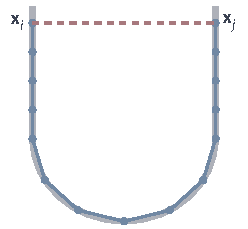
\includegraphics[width=42.012mm]{figures/04-classic-models/00-shared/tikz/dim-geodesic/figure.pdf}
  \caption{一维弯曲曲线上的距离示意。曲线表示嵌入观测空间的一维流形，曲线上的点表示离散样本；沿相邻样本连接的折线表示邻域图路径，其各段长度之和用于近似沿曲线的测地距离。顶部红色虚线是两点间的欧氏直线；若邻域取值过大而把它误纳入图中，就会形成穿过流形外部、低估测地距离的短路。图为几何示意，不是算法输出或实验结果，未给出数值误差。}
  \label{fig:dim-geodesic}
\end{figure}

\subsubsection{参数学习}

暴力建邻域约需$O(n^2d)$时间，空间索引的收益依赖维数与分布。非负边长下，从每点运行二叉堆Dijkstra的成本为$O(n(|E|+n)\log n)$，Floyd--Warshall为$O(n^3)$。后续稠密MDS仍需$O(n^2)$存储、通常$O(n^3)$的完整谱分解；稀疏邻域并未使全体点对距离也稀疏。

输入度量、预处理、$q$或$\varepsilon$以及$k$共同决定结果。小邻域可能断连，大邻域可能跨过卷层，噪声和非均匀采样也会改变可用尺度。可检查连通分量、边长分布及随邻域变化的稳定性。距离相关残差$1-R^2$提供辅助诊断，但对统一缩放不敏感，仍需直接检查失真与测地近似。

\subsubsection{理论分析}
\label{sec:dim-isomap-theory}

\paragraph{表达能力}
Isomap能精确表示的理想对象，是测地距离本来就等于某个$k$维欧氏区域中直线距离的流形。例如一张无拉伸卷起的纸，若参数区域凸，最短纸面路径对应展开后的直线段；图距离恰好等于测地距离时，MDS可以恢复这些展开坐标；图距离仅近似准确时，坐标也仍有相应的近似误差。凸性在这里保证两点之间的直线段没有离开参数区域。带孔区域中的最短路可能绕过孔洞，即使局部平坦，全局测地距离也未必等于展开坐标的直线距离。

并非每个低维流形都有这种全局欧氏表示。取圆周上的四个等间隔点，沿圆的相邻距离为$a>0$、相对点距离为$2a$。若欧氏坐标精确保留这些距离，两条长度为$a+a$的路径都必须满足三角不等式取等；两个中间点便都成为同一线段的中点。但它们在圆周上相距$2a$，产生矛盾。因此即使图距离恰好等于真实圆周测地距离，任何欧氏维数也不能同时零失真实现全部点对。实际Isomap还会叠加邻域短路、覆盖不足及MDS截断的误差；前两项改善后，后一项的几何限制仍然存在。

\paragraph{收敛性}
固定图后，最短路径算法求出图距离，经典MDS求相应的谱近似。数值精度可以通过路径与谱求解检查，邻域是否近似真实几何则属于建模条件；计算完成并未消除两层近似的误差。

\paragraph{泛化性}
样本增加时，希望图距离也越来越接近测地距离。覆盖不足会漏掉必要连接，边长失真过大又会形成捷径，下面的确定性界分别控制这两种问题。

覆盖空隙$h$衡量流形上各位置到最近样本的最大测地距离，单边失真$\eta$衡量弦长比测地距离短多少。证明沿最短测地线放置分割点，再用附近样本替代它们，构造图路径以控制误差；这里尚未要求该距离能嵌入指定$k$维。

\begin{lemma}[覆盖条件下的图距离界]
  \label{thm:dim-isomap-bound}
  设$\mathcal{M}\subset\mathbb{R}^d$连通，任意两点间存在最短测地线。样本的测地填充距离为
  \[
    h=\sup_{\bm{x}\in\mathcal{M}}\min_i
      d_{\mathcal{M}}(\bm{x},\bm{x}_i).
  \]
  图连接全部欧氏距离不超过$\varepsilon$的样本对，并以欧氏弦长为边长。假设$h<\varepsilon/2$，且存在$0\leq\eta<1$，使每条边都满足
  \[
    \lVert\bm{x}_i-\bm{x}_j\rVert_2
    \geq(1-\eta)d_{\mathcal{M}}(\bm{x}_i,\bm{x}_j).
  \]
  则对所有样本对，图距离有限，且
  \begin{equation}
    \label{eq:dim-isomap-bound}
    \begin{aligned}
      d_{\mathcal{G}}(i,j)
        &\geq(1-\eta)d_{\mathcal{M}}(\bm{x}_i,\bm{x}_j),\\
      d_{\mathcal{G}}(i,j)
        &\leq\left(1+\frac{2h}{\varepsilon-2h}\right)
          d_{\mathcal{M}}(\bm{x}_i,\bm{x}_j).
    \end{aligned}
  \end{equation}
\end{lemma}
\begin{proof}
  对任意图路径，各边弦长至少是对应测地距离的$1-\eta$倍。将其相加，再用测地距离的三角不等式，就得到下界。

  为证明上界，记两端点的测地距离为$L$，取连接它们的一条最短测地线，令$a=\varepsilon-2h>0$。若$L=0$，结论成立；否则沿测地线每隔$a$放一个分割点，末段不足$a$，总段数为$s=\lceil L/a\rceil$。保留原来的两个样本端点，把每个内部分割点替换成测地距离不超过$h$的样本。相邻替代样本的测地距离至多$a+2h=\varepsilon$，欧氏距离不更大，因此构成图中的边；重复样本可略去。

  每个内部分割点的替代误差至多在两条相邻边中各计一次，而两端点无需替代，故所构造路径的长度至多
  \[
    L+2h(s-1)
    \leq L+\frac{2hL}{\varepsilon-2h}.
  \]
  图最短路径不长于这条路径，得到上界，同时证明图中这些端点相连。
\end{proof}

对一列样本与邻域，若$h/\varepsilon\to0$且$\eta\to0$，两侧界给出样本点对上的统一相对距离一致性。曲率有界仍需配合足够小的邻域尺度，才能排除卷层间连接。若采样独立且密度有正下界，可以研究覆盖空隙$h$的概率界，条件还需包括体积、内在维数、覆盖数和密度。

还可以把覆盖条件转成新点对的期望风险。

\begin{theorem}[Isomap在覆盖与无短路条件下的期望测地距离误差界]
 \label{thm:dim-isomap-risk}
设$\mathcal M$紧致，测地直径至多为已知常数$D$；训练样本独立同分布于$P$，$P$的支持为$\mathcal M$。假设流形上任意欧氏距离不超过$\varepsilon$的点对均满足前述图距离引理中的无短路条件。对独立新点$\bm x,\bm x'$，冻结训练边，将两个查询节点按同一半径接入图，并保留满足半径条件的查询间边；以该图的最短路径$d_n(\bm x,\bm x')$预测测地距离。为使覆盖失败时的风险也有限，取$\widehat d_n=\min\{d_n,D\}$，不连通时约定$\widehat d_n=D$。

用$N_h$个测地半径$h/2$的球覆盖$\mathcal M$，并假设每个覆盖球的$P$质量至少为$p_h>0$，其中$h<\varepsilon/2$。任一球未包含训练点的概率至多为$e^{-np_h}$；所有球均有样本时，填充距离至多为$h$。查询节点加入后仍保持这一覆盖，引理\ref{thm:dim-isomap-bound}给出新点对上的距离误差。因此，令
$\beta_h=\max\{\eta,2h/(\varepsilon-2h)\}$，有
\begin{equation}
 \mathbb E_{D_n}\mathbb E_{\bm X,\bm X'\sim P}
  [\widehat d_n(\bm X,\bm X')-d_{\mathcal M}(\bm X,\bm X')]^2
 \leq D^2\beta_h^2+D^2N_h e^{-np_h}.
 \label{eq:dim-isomap-risk}
\end{equation}
\end{theorem}

内层两个新点独立同分布且独立于训练集。覆盖事件上，双侧距离界使误差至多$D\beta_h$；失败事件上，截断使误差至多$D$，再用覆盖球的并集界得到该式。这是图距离估计阶段的期望风险，尚未包括后续低维欧氏嵌入的失真。

图距离准确之后，还要判断是否存在欧氏坐标保留它。单位球面赤道上四个等间隔点，相邻测地距离为$\pi/2$，两组对点为$\pi$。若都能成为欧氏距离，三角不等式取等号迫使另外两点成为同一对点的中点；它们却应相距$\pi$，产生矛盾。这说明真实测地距离本身也可能无法同时欧氏实现。

当流形与$\mathbb{R}^m$中凸区域在长度意义下等距时，区域内测地长度就是直线距离，这是恢复平直坐标的一类充分情形。带孔非凸区域即使局部平直，绕孔长度仍可能不同。后续MDS还需控制距离误差对内积和谱子空间的影响。新点可通过到邻居的边长加训练图距离，再用式\eqref{eq:dim-mds-extension}定位；原图固定，不等于加入点后重新计算全体最短路径。

\subsubsection{优化表达能力}

若局部几何在各方向按同一比例缩放，原始图路径会同时记录这种尺度变化。共形Isomap（Conformal Isomap, C-Isomap）在潜在区域均匀采样的假设下，用观测中的局部近邻距离估计缩放程度，先修正邻域边长，再计算路径和MDS坐标\scite{dimDeSilva2002}。它扩大了允许的局部几何变化，却增加了尺度估计和采样假设；潜在采样本来不均匀时，密度变化可能被误解释为几何缩放。

\subsubsection{优化计算能力}

原始Isomap需要全体点对的图距离，邻域图稀疏也不能免去这部分存储和后续谱计算。标志点Isomap（Landmark Isomap）选$s\ll n$个代表点，只从这些点出发求最短路径，保留$s\times n$距离表，再用标志点MDS和距离扩展安排其余点\scite{dimDeSilva2002}。它减少了距离计算的规模，代表点覆盖不足时，也可能遗漏稀有区域或细窄连接。

\subsubsection{小结}

Isomap将局部边长汇总成全局长度，适合考察可展开的几何结构。覆盖、无短路邻域与目标欧氏维数共同决定可靠性。断连分量之间没有有限路径，需分别处理或依据额外信息连接；随意填入大数会引入新的距离假设。

\subsection{局部线性嵌入（LLE）}
\label{sec:dim-lle}

展开弯曲点集并不一定要拟合全部路径长度。只看一小块足够平滑的区域，它近似一个平面，某个点可以由附近点的仿射组合重构；当这块区域平移或旋转时，同一组组合权重仍然成立。\term{局部线性嵌入}（locally linear embedding, LLE）先为每个样本求这种局部重构权重，再安排低维坐标，使原来的组合关系尽量保留。与Isomap保留路径距离相比，它把约束集中在局部组合上，省去全体点对的最短路径计算。区域较大或曲率较强时，局部线性近似也会留下误差。

LLE与Isomap在2000年同一期《Science》上相邻发表，都利用局部信息建立全局坐标。LLE原文致谢中记载了作者与Tenenbaum的讨论，以及对方提供Isomap代码的帮助\scite{dimRoweis2000}两项工作有实际交流，采用的约束却不同：Isomap拟合路径长度，LLE拟合局部重构关系。

\subsubsection{模型结构}

令$\mathcal{N}_i$包含样本$i$的$q$个邻居。重构矩阵$\bm{W}\in\mathbb{R}^{n\times n}$只在邻居位置取非零权重，且每行权重和为一。通过最小化原空间的重构残差求这些权重：
\begin{equation}
  \label{eq:dim-lle-weights}
  \begin{aligned}
    \min_{\bm{W}}\quad&
      \sum_i\left\lVert\bm{x}_i-\sum_j\bm{W}_{i,j}\bm{x}_j
      \right\rVert_2^2,\\
    \text{满足}\quad&
      \bm{W}\bm{1}=\bm{1},\qquad
      \bm{W}_{i,j}=0\quad(j\notin\mathcal{N}_i).
  \end{aligned}
\end{equation}
行和为一使重构关系对整体平移不变：所有点加上同一个向量，中心点及其重构点同步移动。权重可以为负，因此组合是仿射的，未必是凸的。$\bm{W}$通常不对称，其元素也不能解释为随机游走概率。

固定$\bm{W}$后，在低维空间最小化同一组权重对应的残差。记$\bm{M}=(\bm{I}_n-\bm{W})^{\top}(\bm{I}_n-\bm{W})$，目标为
\begin{equation}
  \label{eq:dim-lle-embedding}
  \begin{aligned}
    \min_{\bm{Z}}\quad&
      \lVert(\bm{I}_n-\bm{W})\bm{Z}\rVert_{\mathrm{F}}^2
      =\operatorname{tr}(\bm{Z}^{\top}\bm{M}\bm{Z}),\\
    \text{满足}\quad&
      \bm{Z}^{\top}\bm{1}=\bm{0},\qquad
      \bm{Z}^{\top}\bm{Z}=n\bm{I}_k.
  \end{aligned}
\end{equation}
样本按行排列，因而残差写作$(\bm{I}_n-\bm{W})\bm{Z}$。中心化约束去掉整体平移，列正交与定范数约束防止坐标全部塌缩。这里选定的是代数尺度，未要求坐标距离等于原始距离。

图\ref{fig:dim-lle-weights}用权重$0.3,0.3,0.4$重构中心点。邻居移动后，以同一权重安排中心仍可得到零残差，三角形边长却已改变。完整LLE还需协调其他点的邻域并满足全局约束，图中只展示一项局部关系。

\begin{figure*}[htbp]
  \centering
  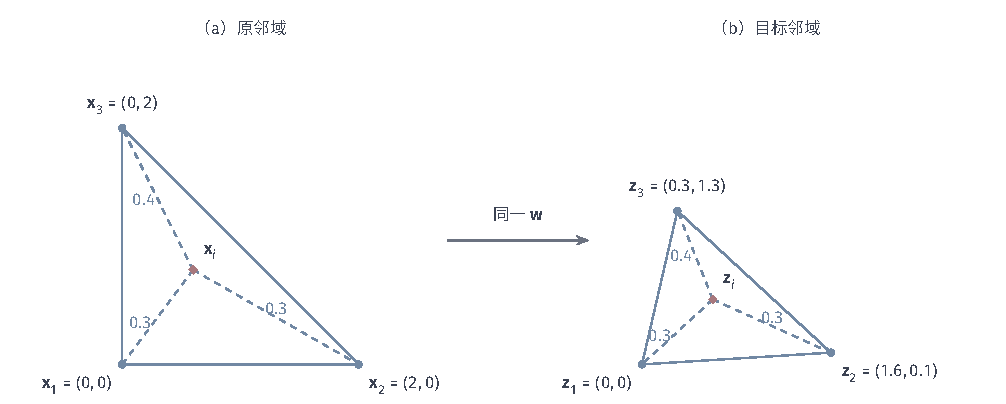
\includegraphics[width=169.000mm]{figures/04-classic-models/00-shared/tikz/dim-lle-weights/figure.pdf}
  \caption{LLE局部权重保持的示意。左图用二维局部坐标绘出三个邻居和菱形中心点；虚线旁为重构权重，其和为1。右图将邻居移至所标位置，同样的权重给出中心$(0.60,0.55)^\top$。两图使用相同的无量纲尺度，实线三角形的形状与边长可以改变。两个画面用于对照高维局部几何与目标邻域，不是完整LLE输出，也不表示一次二维到二维的降维。}
  \label{fig:dim-lle-weights}
\end{figure*}

\subsubsection{参数学习}

按固定顺序排列第$i$个邻域，令$\bm{A}_i\in\mathbb{R}^{q\times d}$的每行为$(\bm{x}_j-\bm{x}_i)^{\top}$，并记$\bm{C}_i=\bm{A}_i\bm{A}_i^{\top}$。该邻域的权重$\bm{w}_i\in\mathbb{R}^q$满足
\[
  \min_{\bm{1}^{\top}\bm{w}_i=1}
    \bm{w}_i^{\top}\bm{C}_i\bm{w}_i.
\]
当$\bm{C}_i$正定时，驻点条件为$\bm{C}_i\bm{w}_i=c\bm{1}$。用权重和为一确定$c$，得到
\begin{equation}
  \label{eq:dim-lle-local}
  \bm{w}_i
  =\frac{\bm{C}_i^{-1}\bm{1}}
         {\bm{1}^{\top}\bm{C}_i^{-1}\bm{1}}.
\end{equation}
求权重时直接解线性方程即可。$q>d$使$\bm{C}_i$必然奇异；即使$q\leq d$，局部样本接近低维切空间也可能造成秩亏或病态。可用$\bm{C}_i+\rho_i\bm{I}_q$改善条件数，例如令$\rho_i$与迹成比例。邻居全部重合时迹为零，需另设正的尺度下限或单独处理。加入正则项也改变了原重构目标。

行和约束给出$\bm{M}\bm{1}=\bm{0}$。在常数方向的正交补中，取最小的$k$个特征方向组成单位列矩阵$\bm{U}_k$，则$\bm{Z}=\sqrt n\,\bm{U}_k$解式\eqref{eq:dim-lle-embedding}。零空间只有常数方向时，才能取最小$k+1$个特征向量后丢掉一个。断连分量的指示向量也属于零空间；对于带符号权重，连通本身仍不足以保证零空间只有一维。

额外零模态会使部分坐标只给各分量分配常数，未表达分量内部的形状。分别嵌入各分量也无法由局部关系确定它们的相对位置、方向和尺度，断连问题仍需额外处理。

局部矩阵构造及求解约需$O(nq^2d+nq^3)$。全局阶段可依次乘$\bm{I}_n-\bm{W}$及其转置，无需显式形成$\bm{M}$；一次矩阵向量乘约为$O(nq)$。部分谱求解还受谱隙、迭代次数和重正交成本影响。邻居数$q$、输出维数$k$与正则尺度都需要选择。

对新点先求局部重构权重，再以$\bm{z}(\bm{x})=\sum_{j\in\mathcal{N}(\bm{x})}w_j(\bm{x})\bm{z}_j$插值。训练坐标固定，这一步未重新求全局谱。邻域不稳定或新点远离训练支持时，插值可能失真。

\subsubsection{理论分析}

\paragraph{表达能力}
固定邻域权重后，LLE要求的是$\bm Z=\bm W\bm Z$，而非点间距离相同。若原数据位于一个$m$维仿射子空间，且每个点的邻居能够仿射重构该点，无正则化的权重可使$\bm X=\bm W\bm X$成立。对数据作中心化和任意线性变换仍保留这个等式；当样本实际张成该空间、$k=m$时，再白化坐标即可同时满足列正交约束，得到零嵌入残差。白化会改变长度与角度，因此零残差本身不表示等距恢复。

一般固定权重未必允许$k$个非平凡的零残差方向。只有$\ker(\bm I_n-\bm W)$在常数方向之外至少还有$k$维，才存在满足本节规范化的零目标表示；否则最小残差为正。光滑流形上的局部仿射关系只能近似成立，后面的Taylor展开说明曲率与权重幅度怎样产生剩余误差。邻域关系也不能确定断连分量之间的位置；对齐或插值不能补回图中未提供的关系。

局部重构关系为何可能在降维后保留，可以用坐标函数的Taylor展开解释。令邻居的局部位移为$\bm{\xi}_j$，对光滑函数$f$有
\[
  \begin{aligned}
    f(\bm{x}_i)-\sum_j\bm{W}_{i,j}f(\bm{x}_j)
    ={}&-\nabla f^{\top}\sum_j\bm{W}_{i,j}\bm{\xi}_j\\
       &+O\left(\sum_j|\bm{W}_{i,j}|
                  \lVert\bm{\xi}_j\rVert_2^2\right).
  \end{aligned}
\]
权重和为一消去常数项，加权位移接近零又使一阶项较小，剩余误差主要来自二阶变化。余项中出现权重绝对值，所以大幅正负抵消可能放大误差。噪声还会改变邻域和局部矩阵，局部近似是否可靠需要另行检查。



\paragraph{收敛性}
每个局部权重问题是带仿射约束的凸二次问题，最小值存在；局部矩阵正定时解唯一，奇异时可能有多个解。加入正的对角正则可以得到唯一权重，但会改变局部重构目标。冻结权重后，$k\leq n-1$时中心化且规范化的坐标集紧致，嵌入最小值存在，并由常数方向正交补中的最小$k$个特征方向达到。截断位置有谱间隔时，最优子空间唯一，坐标仍允许正交旋转。求特征向量的迭代速度依赖谱间隔与求解器；两阶段求解的精确性也不表示它在联合优化权重与坐标。

\paragraph{泛化性}
固定邻域权重后，令$I$在训练索引中均匀抽取，LLE的局部关系风险为
\[
 R_G(\bm Z)=\mathbb E_I\left\lVert\bm z_I
                 -\sum_jW_{I,j}\bm z_j\right\rVert_2^2
            =\frac1n\operatorname{tr}(\bm Z^\top\bm M\bm Z).
\]
在式\eqref{eq:dim-lle-embedding}的约束下，记常数方向正交补中最小的$k$个特征值为$\nu_1,\ldots,\nu_k$。谱解达到
$R_G^\star=\sum_{\ell=1}^k\nu_\ell$；若完整目标的数值误差为$e_G$，则
$R_G(\widehat{\bm Z})\leq\sum_{\ell=1}^k\nu_\ell+e_G/n$。
这个期望只对固定对象集上的随机索引取平均，不能称为独立新点风险。局部插值规定了新点编码，但若未另外规定总体目标坐标函数、采样密度与权重稳定条件，就没有从训练残差到新点重构或几何损失的界。Hessian LLE与LTSA改变局部目标，同样需按各自目标分析，不能套用本节的特征值和。

\subsubsection{优化表达能力}

\paragraph{约束展开坐标的局部曲率}
LLE保留局部的一阶组合关系，还可以进一步约束坐标在局部怎样弯曲。Donoho与Grimes在2003年提出的\term{Hessian LLE}（Hessian特征映射）估计局部坐标函数的二阶变化，寻找其平方积分接近零的方向。这样做的依据是：连通且局部等距于欧氏区域等条件下，展开坐标在局部为仿射函数，Hessian为零。原理论允许某些非凸、带孔参数区域，但未涵盖任意带孔流形；估计二阶项还需足够且分布合适的邻居，采样要求通常比一阶拟合更强\scite{dimDonoho2003}。在$m$维展开区域对应的连续理想模型中，常数与$m$个展开坐标张成$m+1$维零空间，排除常数后即可恢复展开表示；有内在曲率的流形未必具有这些零Hessian坐标，有限样本中估计到的小特征值也还包含邻域和求谱误差。

\paragraph{协调邻域之间的坐标方向}
弯曲点集的各小块可以分别近似为平面，但不同小块的平面朝向不同，局部PCA坐标不能直接拼在一起。Zhang与Zha在2004年的\term{局部切空间对齐}（local tangent space alignment, LTSA）中，在邻域内估计$m$维切空间及局部坐标，再寻找一组全局坐标，使它们经过各邻域的仿射变换后与局部坐标对齐。重叠邻域提供了拼接所需的共同样本，切空间估计与邻域选择的误差也会传到全局\scite{dimZhang2004}。若目标全局坐标与每块局部坐标之间确实有一致的仿射关系，候选对齐就能做到零残差；若局部弯曲在所选尺度下不可忽略，仿射变换只能近似它。重叠不足时，各块的位置还可分别改变，局部精确并不唯一确定整体表示。

\subsubsection{小结}

LLE保留样本与邻居之间的仿射重构关系，再让这些局部关系共同约束坐标。邻域尺度和局部秩影响权重，权重是否稳定也影响不同小块怎样拼接；局部残差小不能单独说明整体几何已经保留。

Hessian LLE进一步使用局部二阶变化，回应展开坐标应怎样弯曲的问题，同时需要更充分的局部采样。LTSA改为估计并对齐邻域切空间，让重叠样本连接各块坐标，同时增加局部方向估计及对齐误差。两者改变了局部目标，选择时应检查数据支持的是仿射重构、局部等距展开还是切空间拼接。

\subsection{拉普拉斯特征映射（Laplacian Eigenmaps）}
\label{sec:dim-le}

局部信息也可以只说明“这两个样本应当靠近”，而不要求给出路径长度或重构权重。例如，相邻时刻的观测若变化平缓，我们希望它们的低维坐标也平缓变化。\term{拉普拉斯特征映射}（Laplacian Eigenmaps）给相似点连边，对边两端的坐标差施加平方惩罚；边权越大，分开这两个点的代价越大。若只有这项惩罚，把全部点放在同一处就会得到零值，所以还需中心化与尺度约束防止塌缩。Belkin与Niyogi在NIPS 2001介绍相关谱方法，2003年期刊论文展开其模型与几何联系\scite{dimBelkin2003}它与第\ref{sec:clustering-spectral}节的谱聚类共享图拉普拉斯与低频特征方向，直接输出连续坐标，谱聚类则继续将这些坐标转为簇分配。

\subsubsection{模型结构}

在对称邻域图上设非负权重$\bm{W}_{i,j}$。相邻点可取$\exp(-\lVert\bm{x}_i-\bm{x}_j\rVert_2^2/(4\tau))$或$1$，其他位置为零，$\tau>0$控制衰减尺度。令$b_i=\sum_j\bm{W}_{i,j}$、$\bm{D}_b=\operatorname{diag}(b_1,\ldots,b_n)$，图拉普拉斯为$\bm{L}=\bm{D}_b-\bm{W}$。对标量信号$\bm{f}\in\mathbb{R}^n$，由对称性有
\begin{equation}
  \label{eq:dim-le-energy}
  \bm{f}^{\top}\bm{L}\bm{f}
  =\frac12\sum_{i,j}\bm{W}_{i,j}(f_i-f_j)^2.
\end{equation}
能量非负，故$\bm{L}$半正定，常数信号的能量为零。将各坐标列的能量相加，得到
\begin{equation}
  \label{eq:dim-le-objective}
  \begin{aligned}
    \min_{\bm{Z}}\quad&
      \operatorname{tr}(\bm{Z}^{\top}\bm{L}\bm{Z}),\\
    \text{满足}\quad&
      \bm{Z}^{\top}\bm{D}_b\bm{Z}=\bm{I}_k,\qquad
      \bm{Z}^{\top}\bm{D}_b\bm{1}=\bm{0}.
  \end{aligned}
\end{equation}
度加权范数排除零解，加权中心化排除常数方向。缺少后一个约束，就可能将没有区分能力的常数列纳入嵌入。目标只惩罚邻近点的坐标差异，远点是否分开还由全局约束和所选模式决定。

\subsubsection{参数学习}

对坐标列求驻点，在常数的加权正交补中得到$\bm{L}\bm{v}=\lambda\bm{D}_b\bm{v}$。各点度为正时，令$\bm{u}=\bm{D}_b^{1/2}\bm{v}$，将它化成对称特征值问题：
\[
  \bm{L}_{\mathrm{sym}}\bm{u}=\lambda\bm{u},
  \qquad
  \bm{L}_{\mathrm{sym}}
  =\bm{I}_n-\bm{D}_b^{-1/2}\bm{W}\bm{D}_b^{-1/2}.
\]
求得单位向量后，要变回$\bm{v}=\bm{D}_b^{-1/2}\bm{u}$以满足模型的归一化。连通图的广义问题以常数为零特征向量，对称问题的零方向却与$\bm{D}_b^{1/2}\bm{1}$成比例。多个连通分量对应多个零模态，应一并识别；零度点也需单独处理，不能直接作逆度归一化。

若权重矩阵有$O(nq)$个非零元，一次矩阵向量乘为$O(nq)$。总求解成本还包括建图、$k$个方向的迭代及正交化。$q$控制哪些点连接，$\tau$控制连接强弱，$k$控制保留的模式数。过小带宽可能使部分度数接近零，过大带宽则削弱局部差异，可结合图诊断与任务表现选择。

\subsubsection{理论分析}
\label{sec:dim-le-theory}

\paragraph{表达能力}
拉普拉斯坐标能够表示的是选定图上的低频变化。设图连通且各点度为正，把广义特征向量按$\bm D_b$内积归一化，以$\bm v_0$表示常数方向、$\bm v_1,\ldots,\bm v_{n-1}$表示非平凡方向。任何节点信号都可展开为$\bm f=\sum_{\ell=0}^{n-1}a_\ell\bm v_\ell$；若信号只使用前$k$个非平凡模式及常数，它就能由这组表示精确线性重构。舍弃其他模式后的度加权平方误差为$\sum_{\ell>k}a_\ell^2$，依据正是特征方向的加权正交性。

较大的广义特征值对应跨强边变化较快的模式，因而快速切换的标签或局部突变可能在低频截断时丢失。在连通图上，零能量又要求每条正权边的两个端点坐标相同，最终使全部节点重合；本节的非塌缩约束排除了它，所以一个有区分能力的嵌入必须保留正能量。小能量只是图上平滑，没有约束原距离或角度，也不保证不同节点必有不同坐标。

\paragraph{收敛性}
固定非负邻域图后，广义特征值问题给出约束能量的全局最优解。截断处有谱隙时，所选子空间唯一。迭代速度取决于谱隙、预条件和残差要求；有限图上的数值收敛与采样图逼近流形属于不同问题。

\paragraph{泛化性}
拉普拉斯特征映射的原始学习器也只输出训练节点坐标。固定非负对称图，令$S_w=\sum_{i,j}w_{ij}>0$，按$w_{ij}/S_w$抽取有序节点对$(I,J)$，则
\[
 R_G(\bm Z)=\mathbb E\lVert\bm z_I-\bm z_J\rVert_2^2
          =2\operatorname{tr}(\bm Z^\top\bm L\bm Z)/S_w.
\]
在本节的度归一化与常数方向排除约束下，设最小的$k$个可用广义特征值为$\nu_1,\ldots,\nu_k$，谱解的风险为
$R_G^\star=2\sum_{\ell=1}^k\nu_\ell/S_w$。
若迹目标求解误差为$e_G$，则
$R_G(\widehat{\bm Z})\leq R_G^\star+2e_G/S_w$。
这是给定图上的期望邻接损失，未评价独立新点。要把它扩展为总体函数的风险，还须规定延拓、连续能量和采样条件；下面的谱一致性结论解释离散与连续对象的联系，但本身没有给出有限样本的新点损失界。

讨论新样本时，需要将离散能量与连续几何联系起来。式\eqref{eq:dim-le-energy}对应的\term{Dirichlet能量}积分了函数沿流形的变化率平方。采用非负号约定$\Delta_{\mathcal{M}}=-\operatorname{div}_{\mathcal{M}}\nabla_{\mathcal{M}}$，在紧致无边界流形上有
\begin{equation}
  \label{eq:dim-dirichlet}
  \mathcal{E}(f)
  =\int_{\mathcal{M}}\lVert\nabla_{\mathcal{M}}f\rVert_2^2\,\mathrm{d}V
  =\int_{\mathcal{M}}f\Delta_{\mathcal{M}}f\,\mathrm{d}V.
\end{equation}
Laplace--Beltrami算子描述函数沿流形的局部变化，对应欧氏空间的负拉普拉斯。求均值为零、平方积分为一的最平滑函数时，给能量加入约束乘子，并沿光滑扰动$g$求导：
\[
  2\int_{\mathcal{M}}g\Delta_{\mathcal{M}}f\,\mathrm{d}V
  -2\lambda\int_{\mathcal{M}}gf\,\mathrm{d}V
  -2c\int_{\mathcal{M}}g\,\mathrm{d}V=0.
\]
分部积分产生第一项。取$g=1$得到$c=0$，再由扰动任意得到$\Delta_{\mathcal{M}}f=\lambda f$。逐次加入与已有特征函数正交的约束，就按频率从低到高得到函数方向。这一变分关系解释了低频坐标的平滑性。

图与流形之间要分别考察算子和谱。点态收敛作用于固定光滑函数，谱收敛则比较随样本改变的特征值与特征函数，前者不能直接推出后者。Belkin与Niyogi在2006年的谱收敛研究中，分别处理经验算子的谱逼近及小带宽下的连续谱逼近\scite{dimBelkin2006}

\begin{lemma}[一种定性的谱一致性结论]
  \label{thm:dim-le-spectral}
  设$\mathcal{M}$是紧致、连通、无边界的$C^\infty$嵌入$m$维黎曼流形，为简化常数令其体积为一。样本独立均匀采自$\mathcal{M}$。考虑全连接高斯图对应的经验算子
  \[
    \begin{aligned}
      \widehat{\mathcal{L}}_{n,\tau}f(\bm{x})
      ={}&\frac{1}{n\tau(4\pi\tau)^{m/2}}\\
      &\cdot\sum_{j=1}^n
        e^{-\lVert\bm{x}-\bm{x}_j\rVert_2^2/(4\tau)}
        \bigl(f(\bm{x})-f(\bm{x}_j)\bigr).
    \end{aligned}
  \]
  存在趋于零而足够缓慢的带宽序列$\tau_n$，使每个固定的低频特征值依概率收敛到$\Delta_{\mathcal{M}}$的相应特征值。将经验特征向量按该算子延拓并作$L^2(\mathcal{M})$归一化后，孤立单特征值对应的特征函数可在符号对齐后依概率收敛；重特征值应按相应有限维特征子空间比较。
\end{lemma}

该结论针对给定的全连接高斯算子，只断言存在合适带宽序列。归一化幂次用内在维数$m$，且算子未作度归一化。它与模型的广义特征值问题之间还需尺度校正：均匀采样下，度的极限趋向空间常数，可以联系两者；非均匀采样、稀疏截断或流形有边界时，要重新分析度、极限测度及边界条件。

非均匀密度$p$下，未修正的局部能量一般带$p^2$权重，密集区域因而更影响低频表示。谱收敛也未保证少量特征函数组成的映射单射或保留全部距离。新点可用核特征函数延拓，或另学映射。标签传播在给定类别语义下求得分，谱聚类输出簇，本节输出坐标；它们共享图平滑，但目标与评价不同（参见第\ref{sec:classification-label-propagation}、\ref{sec:clustering-spectral}节）。

\subsubsection{小结}

拉普拉斯特征映射用图上的平滑变化组织坐标。邻域权重与归一化决定比较关系，求解时还需处理断连和零模态；坐标适合哪些用途，应回到所建图与原始数据检查。

\subsection{扩散映射（Diffusion Map）}
\label{sec:dim-diffusion}

单条边只记录一对点的关系，更多步的连接还可以描述它们处于怎样的邻域环境。设想在相似度图上随机行走：两点即使没有直接连边，若从它们出发都容易到达同一片区域，也可以被视为接近。\term{扩散映射}（diffusion map）比较两个起点经过相同步数后的到达分布，再把这种分布差异写为低维坐标的距离。较小步数侧重局部连接，较大步数把更多路径纳入比较，也可能抹平局部差异。Coifman与Lafon在2006年建立了这一扩散距离的谱表示，并用时间参数选择尺度\scite{dimCoifman2006}它与拉普拉斯特征映射共享谱计算，但对坐标缩放与点间距离给出了随机行走的含义。

\subsubsection{模型结构}

以对称非负矩阵$\bm{K}$表示原始相似度，可用全连接高斯核或稀疏邻域权重。记原始度为$r_i$，密度重加权后的度为$b_i$，以避免与邻居数$q$混淆。归一化过程为
\begin{equation}
  \label{eq:dim-diffusion-normalization}
  \begin{aligned}
    r_i&=\sum_j\bm{K}_{i,j},&
    \widetilde{\bm{K}}_{i,j}
      &=\frac{\bm{K}_{i,j}}{r_i^\alpha r_j^\alpha},\\
    b_i&=\sum_j\widetilde{\bm{K}}_{i,j},&
    \bm{P}_{i,j}&=\frac{\widetilde{\bm{K}}_{i,j}}{b_i},
    \qquad 0\leq\alpha\leq1.
  \end{aligned}
\end{equation}
假设度数均为正。$\bm{P}$每行和为一，其元素表示一步转移概率。重加权后的度确定平稳分布：
\begin{equation}
  \label{eq:dim-diffusion-stationary}
  \pi_i=\frac{b_i}{\sum_j b_j},
  \qquad
  \pi_i\bm{P}_{i,j}=\pi_j\bm{P}_{j,i}.
\end{equation}
末式是细致平衡关系，故$\bm{\pi}^{\top}\bm{P}=\bm{\pi}^{\top}$。按行写分布与列向量方程$\bm P^\top\bm\pi=\bm\pi$等价（参见\BookSectionRef{sec:rv-markov}{卷2《数学准备：概率、因果与决策》第1章“随机变量”第1.2.5节“历史条件下的状态依赖”}）。平稳分布使用$b_i$；只有$\alpha=0$等特殊情形，才可由原始$r_i$直接计算。

对整数$t\geq0$，以$p_t(i,j)=(\bm{P}^t)_{i,j}$表示$t$步转移概率。定义扩散距离
\begin{equation}
  \label{eq:dim-diffusion-distance}
  D_t^2(i,j)
  =\sum_{a=1}^n\frac{(p_t(i,a)-p_t(j,a))^2}{\pi_a}.
\end{equation}
距离比较整个到达分布，各目标点的差异按平稳概率校正；很少被访问的点上，同样的概率差会计入更大贡献。若两个起点有相同到达分布，距离也会为零，故一般可为伪度量。跨区域瓶颈减缓混合，使部分时间尺度仍能区分这些区域。

图\ref{fig:dim-diffusion-walk}中，两个团只由一条弱边相连。团内传播快，跨团传播慢，4步后大部分概率仍在起点一侧；64步时两行分布已更接近，仍未相同。扩散距离比较这些概率差，节点在示意图中的间隔不参与计算。

\begin{figure}[htbp]
  \centering
  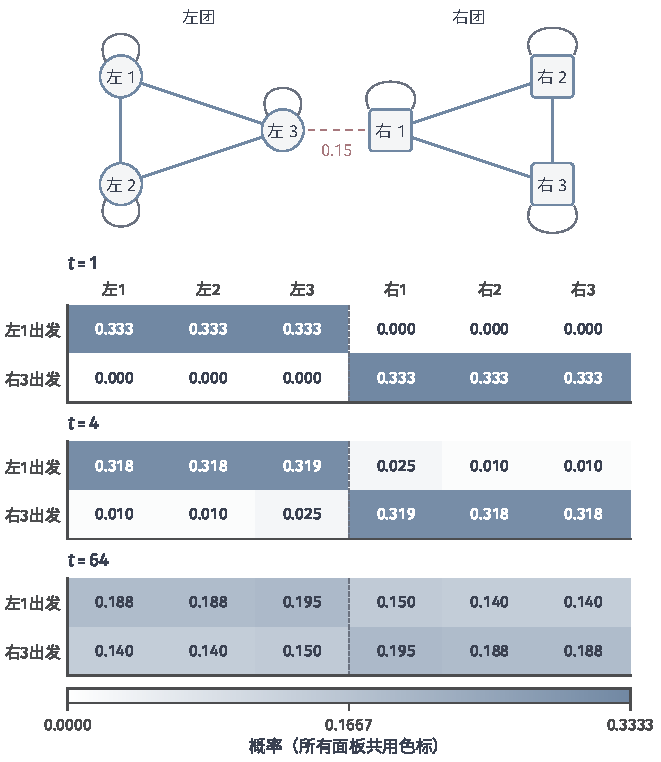
\includegraphics[width=105.412mm]{figures/04-classic-models/00-shared/matplotlib/dim-diffusion-walk/figure.pdf}
  \caption{扩散时间与跨团瓶颈。每团三个节点，团内边及所有自环权重为1，唯一跨团边权重为$0.15$。令$\alpha=0$并按行归一化，热图两行分别表示从左1、右3出发的$\bm{P}^t$对应行，六列为固定节点顺序；各时刻共用同一连续概率色标。数值由有理数矩阵乘法计算，显示三位小数，舍入后行和可能略偏离1。64步仍未充分混合；因图连通且有自环，极限分布均为$\bm{\pi}^{\top}=(20,20,21,21,20,20)/122$。}
  \label{fig:dim-diffusion-walk}
\end{figure}

\subsubsection{参数学习}

记$\bm{\Pi}=\operatorname{diag}(\pi_1,\ldots,\pi_n)$。由细致平衡，矩阵
\[
  \bm{S}=\bm{\Pi}^{1/2}\bm{P}\bm{\Pi}^{-1/2}
\]
为对称矩阵。取其欧氏单位特征向量$\bm{u}_\ell$，并令$\bm{\psi}_\ell=\bm{\Pi}^{-1/2}\bm{u}_\ell$，则
\begin{equation}
  \label{eq:dim-diffusion-eigenvectors}
  \begin{aligned}
    \bm{P}\bm{\psi}_\ell&=\lambda_\ell\bm{\psi}_\ell,\\
    \sum_i\pi_i\psi_\ell(i)\psi_r(i)&=\delta_{\ell,r}.
  \end{aligned}
\end{equation}
这些特征函数在$L^2(\bm{\pi})$内积下正交。连通图的常数特征对为$\lambda_0=1,\psi_0(i)=1$，其余特征值在$[-1,1]$内。再满足非周期性时，非平凡特征值的绝对值小于一。连通图保留正自环即可保证非周期性，无自环二部图却可能出现$-1$特征值。

非负对称权重仍可能有负特征值，应按$|\lambda_1|\geq|\lambda_2|\geq\cdots$选择扩散模态。全连接半正定核经对角缩放仍半正定，此时才可按非负特征值降序选取；稀疏截断可能破坏半正定性。$k$维扩散坐标定义为
\begin{equation}
  \label{eq:dim-diffusion-map}
  \bm{\Psi}_{t,k}(i)
  =\bigl(\lambda_1^t\psi_1(i),\ldots,
         \lambda_k^t\psi_k(i)\bigr)^{\top}.
\end{equation}
将这些坐标按行放置，得到$n\times k$矩阵。$t$对应转移矩阵的整数幂；含负特征值时，直接令$t$取任意实数将失去这一解释。

稠密矩阵的构造、存储及完整谱分解成本与核PCA同阶。稀疏权重降低矩阵向量乘成本，总求谱时间仍受$k$、谱间隔及精度影响。除邻域或带宽与$k$外，还要选择$\alpha$和$t$；同一组谱可在不同$t$下重新加权，无需重复分解。

\subsubsection{理论分析}
\label{sec:dim-diffusion-theory}

\paragraph{表达能力}
扩散映射要表达的是两个起点经过$t$步后到达分布的差异。若两个起点的到达分布相同，扩散距离就是零，表示会将它们视为同一状态，即使原空间中两点相距很远。对给定可逆转移矩阵，保留全部非平凡模态能够精确实现这一距离；保留$k$个模态后的平方失真，是未保留模态的非负贡献之和。下面的定理给出该和及上界，因此可以据谱尾部判断指定维数对这一目标是否足够。

扩散时间改变目标本身。只有需要区分的到达分布差异主要由所保留的慢模态承担，低维截断才会近似保留这些差异；若重要差异来自快速模态，增大$t$反而会把它们抹去。核、密度重加权和步数还改变转移过程，所以精确表达扩散距离并不意味着精确表达欧氏距离或测地距离。

下面在$L^2(\bm{\pi})$中展开转移概率，用正交性消去交叉项，得到有限图上的精确关系与截断界。核尺度与采样图的结构误差仍需另行检查。

\begin{theorem}[扩散映射对固定图扩散距离的表示误差界]
  \label{thm:dim-diffusion-isometry}
  设$\bm{P}$由连通的对称非负权重构造，$\pi_i>0$，特征函数按式\eqref{eq:dim-diffusion-eigenvectors}归一化。对整数$t\geq0$，全部非平凡模态给出
  \begin{equation}
    \label{eq:dim-diffusion-identity}
    D_t^2(i,j)
    =\sum_{\ell=1}^{n-1}\lambda_\ell^{2t}
      \bigl(\psi_\ell(i)-\psi_\ell(j)\bigr)^2.
  \end{equation}
  当$t=0$时按$\bm{P}^0=\bm{I}_n$约定所有模态系数为一。若按特征值绝对值排序，$k<n-1$且$i\ne j$，截断的平方距离误差$R_{t,k}$满足
  \begin{equation}
    \label{eq:dim-diffusion-tail}
    \begin{aligned}
      R_{t,k}(i,j)
        &:=D_t^2(i,j)
          -\lVert\bm{\Psi}_{t,k}(i)-\bm{\Psi}_{t,k}(j)\rVert_2^2,\\
      0\leq R_{t,k}(i,j)
        &\leq|\lambda_{k+1}|^{2t}
          \left(\frac1{\pi_i}+\frac1{\pi_j}\right).
    \end{aligned}
  \end{equation}
\end{theorem}
\begin{proof}
  对称矩阵$\bm{S}$的谱分解给出
  \[
    p_t(i,a)=\pi_a\sum_{\ell=0}^{n-1}
      \lambda_\ell^t\psi_\ell(i)\psi_\ell(a).
  \]
  令$c_\ell=\lambda_\ell^t(\psi_\ell(i)-\psi_\ell(j))$，则$c_0=0$。代入定义，展开平方并使用加权正交性：
  \[
    \begin{aligned}
      D_t^2(i,j)
        &=\sum_a\pi_a
          \left(\sum_{\ell=1}^{n-1}c_\ell\psi_\ell(a)\right)^2\\
        &=\sum_{\ell,r=1}^{n-1}c_\ell c_r
          \sum_a\pi_a\psi_\ell(a)\psi_r(a)
         =\sum_{\ell=1}^{n-1}c_\ell^2.
    \end{aligned}
  \]
  其中$\pi_a$来自分子中$\pi_a^2$除以定义中的$\pi_a$，不能再次消去。截断后余项是$\ell>k$的非负和。由绝对值排序及完整正交基关系，
  \[
    \begin{aligned}
      R_{t,k}
        &\leq|\lambda_{k+1}|^{2t}
          \sum_{\ell=1}^{n-1}
            (\psi_\ell(i)-\psi_\ell(j))^2,\\
      \sum_{\ell=0}^{n-1}\psi_\ell(i)\psi_\ell(j)
        &=\frac{\delta_{i,j}}{\sqrt{\pi_i\pi_j}},
    \end{aligned}
  \]
  对$i\ne j$展开平方，即得所述上界；$i=j$时两种距离和余项都为零。
\end{proof}

保留全部$n-1$个模态时距离精确，截取$k$维则一般有误差。式\eqref{eq:dim-diffusion-tail}同时含谱尾部与平稳概率，稀少区域可能有更大的绝对误差界。增大时间虽使该界缩小，真实扩散距离也随之缩小，不能据此保证相对精度改善。

不可约且非周期的有限链满足$|\lambda_\ell|<1$，故$t\to\infty$时，各起点的到达分布趋于$\bm{\pi}^{\top}$，距离也趋于零。混合前的较大$t$突出慢模态，过大的$t$则丢失区分。连续时间可另用$\exp[-s(\bm{I}_n-\bm{P})]$，以$e^{-s(1-\lambda_\ell)}$加权。

使用同一组对称权重时，拉普拉斯广义问题与转移矩阵满足
\[
  (\bm{D}_b-\bm{W})\bm{v}=\mu\bm{D}_b\bm{v}
  \quad\Longleftrightarrow\quad
  \bm{P}\bm{v}=(1-\mu)\bm{v}.
\]
两者因而共享特征方向。将选定模态的时间权重设为一，并调整归一化，可得到无时间加权的拉普拉斯坐标；$L^2(\bm{\pi})$与$\bm{D}_b$的归一化还差全局尺度。负谱存在时，按绝对值排序的扩散映射可能选中拉普拉斯高端模态，这一选择也需计入比较。

\paragraph{收敛性}
固定满足细致平衡的转移矩阵后，扩散坐标由谱分解求得。残差决定数值精度，谱分离和求解器影响迭代速度。游走时间$t$选择表示尺度，与求谱算法的迭代次数分别控制不同问题。

\paragraph{泛化性}
扩散映射有一个无需总体采样假设的有限图风险结论。固定转移矩阵及$t$，让$I,J$独立按平稳分布$\bm\pi$抽取，用未保留的平方扩散距离作为损失。由定理\ref{thm:dim-diffusion-isometry}及非平凡特征函数的零均值、单位$L^2(\bm\pi)$范数，得到
\begin{equation}
 \mathbb E_{I,J\sim\bm\pi}R_{t,k}(I,J)
 =2\sum_{\ell=k+1}^{n-1}\lambda_\ell^{2t}
 \leq2(n-1-k)|\lambda_{k+1}|^{2t}.
 \label{eq:dim-diffusion-graph-risk}
\end{equation}
每个舍弃模态的两点差平方期望为$2$，所以此处给出精确的平均截断损失，而非仅用最小平稳概率放大的逐点上界。风险仍只对固定图中的节点抽取，未涉及独立新对象；Nystr\"om延拓定义编码以后，还需控制经验转移算子与总体转移算子的误差，才能得到相应总体扩散风险。


密度修正要在采样极限中解释。在光滑正密度$p$、足够采样及小高斯带宽的内点极限下，生成元含有与$2(1-\alpha)\nabla_{\mathcal{M}}\log p$有关的漂移。$\alpha=1$消去主导密度漂移，使极限扩散由流形几何决定；有限样本仍可能有密度影响。$\alpha=0$保留密度作用，适用于任务本身关注该概率结构的情形。

新点可用Nystr\"om方式延拓。沿用训练核及$r_j$，计算$r(\bm{x})=\sum_j\kappa(\bm{x},\bm{x}_j)$，按训练归一化构造$p(\bm{x},j)$。当$\lambda_\ell\ne0$时，有
\begin{equation}
  \label{eq:dim-diffusion-extension}
  \psi_\ell(\bm{x})
  =\frac1{\lambda_\ell}\sum_jp(\bm{x},j)\psi_\ell(j),
  \qquad
  z_\ell(\bm{x})=\lambda_\ell^t\psi_\ell(\bm{x}).
\end{equation}
该式固定训练度和谱，将特征方程延伸到新点。小特征值的倒数会放大误差，零特征值需其他处理。错误连接对传播的影响取决于它如何改变瓶颈，使用多条路径也不能保证减弱每一条错误边的作用。

\subsubsection{优化表达能力}

\paragraph{纳入局部方向关系}

普通扩散映射比较走到哪里的概率，没有同时说明沿路径怎样保持方向。若任务还关心局部切方向在不同区域之间是否一致，就可以把邻域切空间的对齐关系放入传播。Singer与Wu的\term{向量扩散映射}（vector diffusion maps）用正交对齐矩阵记录这些关系，使路径上的方向运输参与比较\scite{dimSinger2012}。其连续对象是作用于向量场的连接拉普拉斯。由这些方向传播关系形成的距离和嵌入，可以区分仅靠标量到达概率没有刻画的局部方向关系；输出仍可采用嵌入坐标，所改进的是表示中保留的信息。

\subsubsection{小结}

扩散映射用多步传播比较样本的到达分布，适合关系需要通过多条局部路径累积的情形。核尺度决定局部联系，重加权调整采样密度的作用，传播时间选择观察粒度；时间过长还可能混合原本要区分的区域，新点延拓则需要沿用训练归一化。

向量扩散映射把切空间对齐加入传播，扩展了嵌入可以利用的几何关系。若研究对象转为图或流形上的函数，Coifman与Maggioni的扩散小波还可用扩散算子的幂构造多尺度函数基，服务于函数近似与算子压缩\scite{dimCoifmanMaggioni2006}。这已经超出本节以低维坐标表示样本的任务，函数基的压缩和正交化需要另作分析。

\subsection{随机邻居嵌入（SNE）}
\label{sec:dim-sne}

同一个距离阈值在稠密区域可能包含许多点，在稀疏区域却只包含一两个点。如果目的是显示每个样本最相关的邻居，就可以先比较它与其他点的相对接近程度，而不要求所有原始距离都按同一比例缩小。Hinton与Roweis于2002年提出\term{随机邻居嵌入}（stochastic neighbor embedding，SNE），为每个样本建立选择邻居的概率分布，再调整低维位置，尽量复现这些概率。局部带宽控制一行分布中的有效邻居数量，使不同疏密区域可以采用不同距离尺度。“随机”指邻居选择的概率模型，坐标仍由优化求得。

原论文用bank的歧义说明表示的局限：河岸与金融是不同语境，单一位置可能难以同时容纳两组邻居。因此作者也讨论了同一对象具有多个位置的混合扩展\scite{dim-hinton2002sne}本节采用单位置形式；邻域分布定义之后，还需判断低维空间能否表达这些关系。

\subsubsection{模型结构}

以$i$为中心，用高斯核将距离转为选择邻居的条件概率：
\begin{equation}
  \label{eq:dim-sne-high}
  \begin{aligned}
    p_{j\mid i}
      &=\frac{\exp(-\delta_{i,j}^2/(2\sigma_i^2))}
      {\sum_{\ell\ne i}\exp(-\delta_{i,\ell}^2/(2\sigma_i^2))},
      \qquad j\ne i,\\
    p_{i\mid i}&=0,\qquad \sum_{j\ne i}p_{j\mid i}=1.
  \end{aligned}
\end{equation}
带宽$\sigma_i>0$决定局部尺度。小带宽将概率集中到近邻，大带宽使远点获得更多权重。两点距离虽对称，条件概率通常不对称，因为各中心的带宽及归一化分母不同。

\term{困惑度}（perplexity）将分布$P_i=(p_{j\mid i})_{j\ne i}$的熵转为有效邻居数，以此校准带宽。采用自然对数时定义
\begin{equation}
  \label{eq:dim-sne-perplexity}
  \begin{aligned}
    H(P_i)&=-\sum_{j\ne i}p_{j\mid i}\log p_{j\mid i},\\
    \operatorname{Perp}(P_i)&=\exp\!\bigl(H(P_i)\bigr).
  \end{aligned}
\end{equation}
概率在$q$个邻居上均匀分配时，困惑度为$q$。一般值可以非整数，未规定固定数量的非零邻居。熵若改用以$2$为底的对数，外层应改为$2^{H_2(P_i)}$。

带宽可根据目标困惑度$\tau$二分搜索。记$\beta_i=1/(2\sigma_i^2)$、$D_j=\delta_{i,j}^2$及$B_i=\sum_{j\ne i}\exp(-\beta_iD_j)$，则
\begin{equation}
  \label{eq:dim-sne-entropy-monotonicity}
  \begin{aligned}
    H(P_i)&=\log B_i+\beta_i\mathbb{E}_{P_i}[D],\\
    \frac{\mathrm{d}}{\mathrm{d}\beta_i}\mathbb{E}_{P_i}[D]
      &=-\operatorname{Var}_{P_i}(D),\\
    \frac{\mathrm{d}H(P_i)}{\mathrm{d}\beta_i}
      &=-\beta_i\operatorname{Var}_{P_i}(D)\leq 0.
  \end{aligned}
\end{equation}
困惑度随带宽单调不减；距离不全相等时严格递增。设并列最近邻有$h_i$个，带宽从零趋向无穷时，困惑度从$h_i$趋向$n-1$，故$\tau\in(h_i,n-1)$才对应唯一有限正带宽。所有距离相等时值恒为$n-1$，重复或并列距离也会限制可达目标。

达到相同困惑度时，稀疏区域通常需更大带宽，稠密区域需更小带宽，所以校准后的邻域分布未直接保留原始密度。可从$5$至$50$探索困惑度，并结合样本数与群体规模调整。预处理仍重要：无关特征改变输入距离后，带宽搜索也会使用这些距离。

低维核尺度固定，坐标通过以下目标学习：
\begin{equation}
  \label{eq:dim-sne-low-loss}
  \begin{aligned}
    q_{j\mid i}
      &=\frac{\exp(-r_{i,j}^2)}
      {\sum_{\ell\ne i}\exp(-r_{i,\ell}^2)},\qquad q_{i\mid i}=0,\\
    C_{\mathrm{SNE}}(\bm{Z})
      &=\sum_i\operatorname{KL}(P_i\Vert Q_i)\\
      &=\sum_i\sum_{j\ne i}p_{j\mid i}
        \log\frac{p_{j\mid i}}{q_{j\mid i}}.
  \end{aligned}
\end{equation}
这里$Q_i=(q_{j\mid i})_{j\ne i}$。核$\exp(-r^2)$与方差为$1/2$、标准差为$1/\sqrt{2}$的高斯密度具有相同形状；固定带宽也就规定坐标单位。共同带宽的改变可由坐标缩放吸收，但在固定带宽下缩放坐标会改变概率与目标。

较大的$p_{j\mid i}$使近邻错置受到较大惩罚：拉远这对点会增加$-\log q_{j\mid i}$。高维远点若挤在低维近处，也会占用归一化概率，减少真正近邻的份额，因而产生排斥作用。整体KL散度非负，单个求和项仍可为负。

\subsubsection{参数学习}

先由$\bm{X}$和$\tau$求带宽并固定$P_i$，再优化坐标。令$A_i=\sum_{\ell\ne i}\exp(-r_{i,\ell}^2)$，以$i$为中心的散度展开为
\begin{equation}
  \label{eq:dim-sne-anchor-loss}
  \begin{aligned}
    C_i&=\sum_{j\ne i}p_{j\mid i}\log p_{j\mid i}
      +\sum_{j\ne i}p_{j\mid i}r_{i,j}^2+\log A_i.
  \end{aligned}
\end{equation}
第一项为常数，第二项按邻居概率拉近点对，第三项反映归一化竞争。求导时必须同时包含后两项，才能得到吸引与排斥共同作用的更新。

$\bm{z}_i$既是$C_i$的中心，也是其他$C_j$的候选邻居。两种贡献分别为
\begin{equation}
  \label{eq:dim-sne-two-roles}
  \begin{aligned}
    \nabla_{\bm{z}_i}C_i
      &=2\sum_{j\ne i}(p_{j\mid i}-q_{j\mid i})
        (\bm{z}_i-\bm{z}_j),\\
    \nabla_{\bm{z}_i}C_j
      &=2(p_{i\mid j}-q_{i\mid j})
        (\bm{z}_i-\bm{z}_j),\qquad j\ne i.
  \end{aligned}
\end{equation}
两个负项分别来自$\log A_i$与$\log A_j$的导数；后者只有含$i$的核项随$\bm{z}_i$变化。将中心与邻居两种贡献相加，得到
\begin{equation}
  \label{eq:dim-sne-gradient}
  \begin{aligned}
    \nabla_{\bm{z}_i}C_{\mathrm{SNE}}
      &=2\sum_{j\ne i}
        \bigl[(p_{j\mid i}-q_{j\mid i})\\
      &\qquad +(p_{i\mid j}-q_{i\mid j})\bigr]
        (\bm{z}_i-\bm{z}_j).
  \end{aligned}
\end{equation}
系数为正时，负梯度更新将$i$拉向$j$；系数为负时将两点推开。因此力的方向由负梯度确定，且需合计两个有向残差，它们可能相互抵消。

用正学习率$\eta_t$作更新$\bm{Z}^{(t+1)}=\bm{Z}^{(t)}-\eta_t\nabla C_{\mathrm{SNE}}(\bm{Z}^{(t)})$，也可加入动量。原工作使用逐渐减弱的随机扰动改善布局，但未保证全局最优。小随机点云能打破全部坐标重合时的对称零梯度状态。

计算完整高维距离需$O(n^2d)$时间，保存概率需$O(n^2)$空间。输出维数固定时，每轮优化为$O(n^2)$。可结合目标值、梯度或位移判断数值进展，再检查近邻保留；数值停止变化只说明当前优化状态。

\subsubsection{理论分析}
\label{sec:dim-sne-theory}

\paragraph{表达能力}
SNE能否精确匹配邻域关系，要看目标条件概率能否由同一组$k$维欧氏距离产生。目标值为零当且仅当每行$Q_i=P_i$。由式\eqref{eq:dim-sne-low-loss}取对数，精确匹配要求存在每行的常数$c_i$，使
\[
 r_{i,j}^2=-\log p_{j\mid i}+c_i\qquad(i\ne j),
\]
且这些数同时构成一个$k$维欧氏平方距离矩阵。它们必须非负、对称，并满足经典MDS的半正定与秩条件；只为每行单独安排邻居，不能保证这些条件同时成立。若高维条件概率原本由某个$k$维点集及统一带宽产生，坐标缩放便可精确匹配；逐点带宽不同或目标维数不足时，则可能留下正的KL误差。

概率目标强调邻域份额，未要求恢复原始距离或采样密度。改变各点带宽已经改变距离到概率的换算，因此即使概率匹配很好，也不能将簇间间距直接读作原空间间距。

\term{拥挤问题}（crowding problem）来自高维邻域与低维空间容量的差异。局部均匀采样于$m$维流形、尺度足够小且远离边界时，半径$r$内样本数近似随$r^m$增长，$k$维体积则随$r^k$增长。这里用的是内在维数$m$；这一比较提供直觉，实际计数还依赖数据与尺度。

$m>k$时，许多中距离关系可能争夺有限位置，高斯核快速衰减进一步限制布局。图\ref{fig:dim-neighbor-tails}中，$r=3$时高斯核约为$0.00012$，Cauchy形核为$0.1$，后者在较远位置仍保留相似度。图中是核值，归一化后的概率还取决于其他点。

\begin{figure}[htbp]
  \centering
  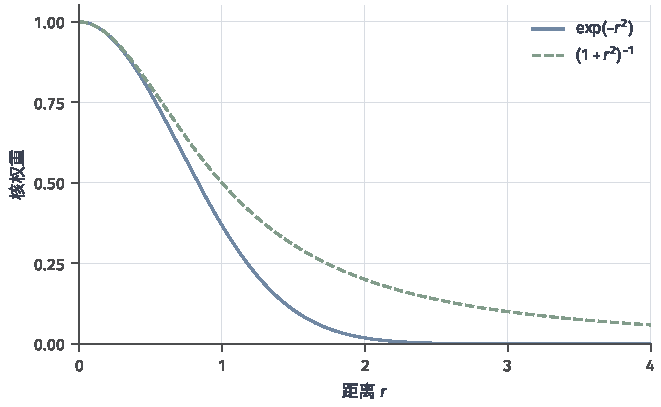
\includegraphics[width=105.412mm]{figures/04-classic-models/00-shared/matplotlib/dim-neighbor-tails/figure.pdf}
  \caption{高斯核$\exp(-r^2)$与Cauchy形核$1/(1+r^2)$的尾部。横轴$r$为无量纲距离，纵轴为未归一化核值，非概率密度、非实验结果；尾部形状本身不保证嵌入保真。}
  \label{fig:dim-neighbor-tails}
\end{figure}

\paragraph{收敛性}
坐标目标非凸，平移、旋转和反射也使坐标解不唯一。梯度光滑且步长合适时，可研究下降与趋近驻点；任意初始化的全局收敛仍无保证。即使谱方法全局解出固定图的子问题，图是否表达真实几何也要另行判断。

\paragraph{泛化性}
标准SNE没有共享输入映射，输出的是固定样本的坐标。其KL目标可以解释为该对象集上的邻居预测风险：先均匀抽取$I$，再按高维条件分布$p_{j\mid I}$抽取邻居$J$，用低维概率预测这一选择。交叉熵风险满足
\[
 R_G(\bm Z)=\mathbb E[-\log q_{J\mid I}]
 =\frac1n\sum_iH(p_{\cdot\mid i})+\frac1nC_{\mathrm{SNE}}(\bm Z).
\]
固定高维分布后，熵项不随坐标改变；若KL目标距全局最小值至多为$e_G$，就有
$R_G(\widehat{\bm Z})\leq\inf_{\bm Z}R_G(\bm Z)+e_G/n$。
该风险中的随机对象是已有样本索引，不能把训练样本间的$n(n-1)$个关系视作独立新观测。要处理新点，须另定参考邻域、旧坐标是否固定，以及新点损失；原始KL目标没有给出这种扩展的总体保证。输入关系主要来自噪声时，充分优化仍可能只是保留噪声关系。

\subsubsection{小结}

SNE先以困惑度校准邻域，再以条件概率和KL散度学习坐标。表示能力、布局优化和点对计算各有约束：更换核、改进优化与计算加速分别解决不同问题，需要分别评价。

\subsection{t-SNE}
\label{sec:dim-tsne}

SNE在低维空间用高斯距离构造邻居概率，高斯核随距离迅速衰减。高维中，一批点可以都离中心不远，彼此却分布在许多不同方向；把它们放到二维时，很难同时保留这些接近关系。若为了维持中等的相似度把许多点拉向中心，它们就会相互挤近，这就是拥挤问题的一种表现。

van der Maaten与Hinton于2008年提出\term{t-SNE}（t-distributed stochastic neighbor embedding），把低维核换为衰减较慢的重尾形式，并将逐点条件分布改为对称点对分布\scite{dim-vandermaaten2008tsne}重尾核允许中等相似度的点对在低维中相距更远，从而给重要近邻留下布局空间；对称化则让两个方向的邻居关系进入同一项损失。这些改变缓解了布局限制，却没有使二维坐标成为所有高维距离的等比例缩小。

\subsubsection{模型结构}

沿用高维条件概率与困惑度，为每对样本构造一个对称权重：
\begin{equation}
  \label{eq:dim-tsne-joint}
  \begin{aligned}
    p_{i,j}&=\frac{p_{j\mid i}+p_{i\mid j}}{2n},\qquad i\ne j,\\
    p_{i,i}&=0,\qquad p_{i,j}=p_{j,i},\qquad
      \sum_{i\ne j}p_{i,j}=1.
  \end{aligned}
\end{equation}
求和包括有序对的两个方向。$n$个条件分布各归一化为$1$，两方向相加后的总和为$2n$，因此分母取$2n$。若改按$i<j$求和，归一化及后续导数系数也需调整。

低维点对采用Cauchy形核，并在全部有序对上归一化：
\begin{equation}
  \label{eq:dim-tsne-low}
  \begin{aligned}
    u_{i,j}&=(1+r_{i,j}^2)^{-1},\qquad
      \mathcal{Z}=\sum_{a\ne b}u_{a,b},\\
    q_{i,j}&=\frac{u_{i,j}}{\mathcal{Z}},\qquad i\ne j,\\
    q_{i,i}&=0,\qquad \sum_{i\ne j}q_{i,j}=1.
  \end{aligned}
\end{equation}
$u_{i,j}$具有自由度为$1$的一维Student $t$核形状，$q_{i,j}$则是有限点对上的离散概率。重尾允许较远点获得相似度，未规定高低维距离相等，也未将$q_{i,j}$定义为$\mathbb{R}^k$上的多元Cauchy密度。

记$\bm{P}=(p_{i,j})$、$\bm{Q}=(q_{i,j})$，以点对分布间的KL散度学习坐标：
\begin{equation}
  \label{eq:dim-tsne-loss}
  C_{\mathrm{tSNE}}(\bm{Z})
    =\sum_{i\ne j}p_{i,j}\log\frac{p_{i,j}}{q_{i,j}}.
\end{equation}
全部点对共享归一化常数$\mathcal{Z}$。移动一个点会改变它和其他点的核值，也改变其余点对的概率，所以坐标要在共同概率预算下协调。

高概率近邻错置受到较大惩罚，簇间距离、面积和密度却未被要求复原。小$p_{i,j}$的吸引弱，但这些点对仍参与归一化与斥力计算，局部目标也需要考虑远点。

\subsubsection{参数学习}

代入低维核并利用$\sum_{i\ne j}p_{i,j}=1$，展开目标与归一化项的梯度：
\begin{equation}
  \label{eq:dim-tsne-gradient-derivation}
  \begin{aligned}
    C_{\mathrm{tSNE}}
      &=\text{常数}
        +\sum_{a\ne b}p_{a,b}\log(1+r_{a,b}^2)
        +\log\mathcal{Z},\\
    \nabla_{\bm{z}_i}\mathcal{Z}
      &=-4\sum_{j\ne i}u_{i,j}^2(\bm{z}_i-\bm{z}_j),\\
    \nabla_{\bm{z}_i}\log\mathcal{Z}
      &=-4\sum_{j\ne i}q_{i,j}u_{i,j}(\bm{z}_i-\bm{z}_j).
  \end{aligned}
\end{equation}
距离平方的导数贡献因子$2$，有序对的两个方向再贡献因子$2$。吸引项同理给出$4\sum_{j\ne i}p_{i,j}u_{i,j}(\bm{z}_i-\bm{z}_j)$，因此
\begin{equation}
  \label{eq:dim-tsne-gradient}
  \nabla_{\bm{z}_i}C_{\mathrm{tSNE}}
    =4\sum_{j\ne i}(p_{i,j}-q_{i,j})u_{i,j}
      (\bm{z}_i-\bm{z}_j).
\end{equation}
$p_{i,j}>q_{i,j}$时，负梯度拉近点对，反之推开。即使稀疏近似中$p_{i,j}=0$，有限距离的$q_{i,j}$仍为正，因而仍有斥力。每个点的位移由全部点对作用合成。

\term{早期夸大}（early exaggeration）在初始阶段将梯度中的$p_{i,j}$乘以$\alpha>1$，增强吸引后再恢复$\alpha=1$。原文使用$4$，后续也常用$12$，但需与学习率及样本数配合。夸大后权重和为$\alpha$，该阶段的更新已不是原归一化分布间KL散度的梯度。

初始化和动量也影响优化。缩放后的PCA坐标提供结构化起点，随机点云则不带这一信息；因此宏观布局差异可能同时来自起点与目标。动量未保证逃离局部极小值。实验应记录困惑度、学习率、初始化和夸大系数及轮数。

\subsubsection{理论分析}
\label{sec:dim-tsne-theory}

\paragraph{表达能力}
t-SNE扩大了中距离关系可以使用的布局范围，却仍通过同一组欧氏坐标耦合全部点对。若目标值为零，就必须有$q_{i,j}=p_{i,j}$；由式\eqref{eq:dim-tsne-low}可得
\[
 r_{i,j}^2=\frac{1}{\mathcal Z p_{i,j}}-1\qquad(i\ne j).
\]
因此只有存在一个共同的$\mathcal Z>0$，使这些平方距离经双中心化后得到的Gram矩阵半正定且秩至多为$k$，全部概率才能精确匹配。反过来，若这些距离可实现，核值为$\mathcal Zp_{i,j}$，全点对归一化就恰好恢复$\bm P$。重尾改变了概率对应的距离，却没有免除这一共同的几何约束。

高维高斯邻域经对称化后得到的目标概率，并不自动满足上述条件，二维或三维目标因而可能只能近似拟合。由于拟合对象是经过尺度调整的点对概率，视觉上分离的簇、簇面积和间距都可能来自布局目标，原空间未必具有相同密度或距离比例。

\paragraph{收敛性}

坐标目标仍非凸。Linderman与Steinerberger在2019年SIAM期刊论文中，针对有适当簇结构的输入相似度、集中初始点云及满足条件的步长和夸大系数，分析早期簇内收缩与谱聚类的联系\scite{dim-linderman2019clustering}结论针对该阶段和条件，未覆盖任意数据的整个训练。

初始间距小时，$u_{i,j}\approx1$。若斥力扰动相对较小并暂不计动量，更新近似为
\begin{equation}
  \label{eq:dim-tsne-spectral-approximation}
  \begin{aligned}
    \bm{Z}^{(t+1)}
      &\approx(\bm{I}-4\eta_t\alpha\bm{L}_{P})\bm{Z}^{(t)},\\
    \bm{L}_{P}&=\bm{D}_{P}-\bm{P},\qquad
    (\bm{D}_{P})_{i,i}=\sum_{j\ne i}p_{i,j}.
  \end{aligned}
\end{equation}
对角矩阵$\bm{D}_{P}$记录行和。步长合适时，图平滑抑制快速变化方向，因而与拉普拉斯谱相联系。点云展开后，核值接近$1$的近似会减弱，斥力也更不可忽略；关闭夸大后，布局仍由两种作用共同调整。

\paragraph{泛化性}
固定高维联合点对分布$p_{ij}$，抽取$(I,J)\sim p$后用$q_{ij}(\bm Z)$预测，交叉熵风险为
\[
 R_G(\bm Z)=\mathbb E_{(I,J)\sim p}[-\log q_{IJ}(\bm Z)]
           =H(p)+C_{\mathrm{tSNE}}(\bm Z).
\]
所以完整KL目标距全局最小值至多为$e_G$时，有
$R_G(\widehat{\bm Z})\leq\inf_{\bm Z}R_G(\bm Z)+e_G$。
这是固定对象集的点对风险，较小训练KL只回答该邻居预测任务；点对分布由同一批数据产生，不能据此断言独立新点上的期望风险小。参数化t-SNE虽然给出了输入映射，还需规定总体点对采样与归一化制度，并控制函数族的复杂度；前向计算本身没有提供风险界。


困惑度决定输入分布，也决定所求问题。小值强调细邻域，可能割裂连续结构；大值引入更广关系，可能模糊稀有群体。可在可达范围内比较$5$、$30$、$50$等尺度及多次初始化，寻找稳定关系。不同困惑度对应不同目标分布，其KL值不能直接用于排名。

旋转和镜像通常不改变解释，簇间距、面积及疏密却也不能直接换算为原空间量。布局可能展开大簇、压紧小簇，或将连续变化分成区域。单细胞、文本或图像特征中的分组应回到合适的高维表示验证，并分别考察内部指标、稳定性、参考标签及下游效果（参见第\ref{sec:clustering-summary}节）。

\subsubsection{优化计算能力}

原始算法每轮需$O(n^2)$计算。van der Maaten在2014年的Barnes--Hut t-SNE中将吸引图稀疏化，并用低维树聚合远点、近似斥力，二维常用四叉树。固定近邻预算及近似精度、输出维数较小时，每轮典型成本为$O(n\log n)$；建图及极端布局仍会影响时间\scite{dim-vandermaaten2014accelerating}

Linderman等在2019年的FIt-SNE中通过网格插值和快速傅里叶变换加速核求和\scite{dim-linderman2019fitsne}。固定插值阶数时，斥力成本约为$O(n+g\log g)$，其中$g$为网格节点数，此外还需计算稀疏吸引。范围与精度改变时$g$也会改变。2019年工作展示了百万级单细胞数据的处理，实际规模与收益仍依赖计算条件。

\subsubsection{支持新样本低维编码场景}

新点需要额外扩展规则。openTSNE等实现固定参考坐标，再按新点与参考样本的相似度优化新坐标\scite{dim-policar2024opentsne}。这是条件定位，与新旧样本联合训练不同；参考集未覆盖的新群体可能被安排到失真位置。

需要反复处理新样本时，可令$\bm{z}_i=f_{\bm{\theta}}(\bm{x}_i)$，按邻域目标学习共享参数。van der Maaten于2009年提出参数化t-SNE，以前向计算表示新点\scite{dim-vandermaaten2009parametric}。网络函数族限制可实现布局，批次构造与归一化也影响训练关系。

\subsubsection{小结}

t-SNE用对称点对分布和重尾核组织局部相似性，适合探索邻域。它重视保留高概率关系，簇间距离、面积和疏密却不宜直接换算成原空间量；困惑度与初始化也会改变所显示的结构。

计算加速与新点编码处理不同瓶颈。Barnes--Hut用树近似远点作用，FIt-SNE用网格插值加速核求和，两者都需选择近似精度。固定参考表示后优化新点，可以复用既有坐标；参数化t-SNE改为学习共享输入函数，减少逐点定位，同时让函数族与训练方式限制可实现布局。这些调整方便计算和使用，结构解释仍需回到原表示验证。

\subsection{UMAP}
\label{sec:dim-umap}

SNE和t-SNE把邻域相似度组成归一化概率分布，目标是匹配这些分布。另一种表示方式是直接为每条局部连接赋予强度：两个样本在各自邻域里有多接近，就决定这条连接有多强，全部点对的权重不需要加起来等于1。\term{统一流形逼近与投影}（uniform manifold approximation and projection，UMAP）先按各点的局部距离尺度建立加权邻域，再合并两端对同一连接的判断，得到一张稀疏图。低维布局随后拟合这些连接强度，让强连接的点靠近，并对其他点对施加排斥。它延续了邻域表示的目标，但改变了高维关系的构造与拟合方式。

McInnes、Healy与Melville自2018年公开的方法长文，将拉普拉斯特征映射、黎曼几何与模糊拓扑联系起来，讨论非均匀样本的局部度量及其合并\scite{dim-mcinnes2018umap}这一构造也面向较高维预处理。方法长文与同年JOSS软件论文分别描述理论构造和实现，几何解释、实现行为与可视化效果应各自评价。

\subsubsection{模型结构}

以$N_q(i)$表示不含$i$的$q$个近邻。先取互异样本、无并列最近邻及单位局部连接设置。记$\rho_i=\min_{j\ne i}\delta_{i,j}$，定义有向权重
\begin{equation}
  \label{eq:dim-umap-directed}
  \begin{aligned}
    v_{j\mid i}
      &=
      \begin{cases}
        \exp\!\left(-\dfrac{\max(0,\delta_{i,j}-\rho_i)}
        {\sigma_i}\right),&j\in N_q(i),\\
        0,&j\notin N_q(i),
      \end{cases}\\
    \sum_{j\in N_q(i)}v_{j\mid i}&=\log_2 q.
  \end{aligned}
\end{equation}
偏移$\rho_i$使最近邻权重为$1$，带宽$\sigma_i$控制其余边衰减。上述条件下，$q>2$时权重和随带宽从$1$趋向$q$，可搜索满足目标的带宽。距离可按任务更换，相应的几何解释也需要调整。

这些值是边的隶属强度，多条边可同时很强。校准目标$\log_2 q$未将行和设为$1$，也未使用熵或困惑度。重复或并列样本、其他局部连接设置可能使多条边固定为$1$，导致目标不可达，因而实现还需处理零距离、带宽下界与容差。

用模糊并将两个方向合成对称权重：
\begin{equation}
  \label{eq:dim-umap-union}
  v_{i,j}=v_{j\mid i}+v_{i\mid j}-v_{j\mid i}v_{i\mid j}.
\end{equation}
所得$v_{i,j}=v_{j,i}\in[0,1]$。一方向为$1$则合并为$1$，两方向均为$0.4$则合并为$0.64$。这是模糊集合运算，无需把两条边假定为独立事件。

\term{模糊单纯集}（fuzzy simplicial set）将点、边和三角面等组合结构赋予隶属强度，提供局部描述的组合框架。实际目标主要使用样本与加权边，即一维骨架。有限图中的环和空白是否对应真实拓扑，仍需采样与几何证据。

低维边强度由可调重尾核给出：
\begin{equation}
  \label{eq:dim-umap-kernel}
  w_{i,j}=\frac{1}{1+a r_{i,j}^{2b}},\qquad a>0,\quad b>0.
\end{equation}
由\code{min\_dist}和\code{spread}选择$a,b$，使光滑核逼近近处接近$1$、超过指定尺度后衰减的曲线。\code{min\_dist}允许控制紧凑程度，未给每对点施加硬距离下界。$a=b=1$时核形与t-SNE的$u_{i,j}$相同，但没有全局归一化，因而与$q_{i,j}$不同。

将每条边视为带软标签的二元判断，就可以匹配高低维边强度。按无序对$i<j$写完整目标：
\begin{equation}
  \label{eq:dim-umap-bernoulli}
  \begin{aligned}
    C_{\mathrm{B}}(\bm{Z})
      &=\sum_{i<j}\left[
        v_{i,j}\log\frac{v_{i,j}}{w_{i,j}}\right.\\
      &\qquad\left.+
        (1-v_{i,j})\log\frac{1-v_{i,j}}{1-w_{i,j}}
        \right].
  \end{aligned}
\end{equation}
该式求和逐边Bernoulli分布的KL散度。去掉只依赖高维权重的常数，得到二元交叉熵：
\begin{equation}
  \label{eq:dim-umap-cross-entropy}
  \begin{aligned}
    C_{\mathrm{CE}}(\bm{Z})
      &=-\sum_{i<j}\left[
        v_{i,j}\log w_{i,j}\right.\\
      &\qquad\left.+
        (1-v_{i,j})\log(1-w_{i,j})\right].
  \end{aligned}
\end{equation}
采用$0\log0=0$。两式对坐标有相同梯度，所以与t-SNE的核心区别在匹配对象：这里逐边二元匹配，t-SNE匹配全局归一化的点对分布。

正边项吸引，非边项排斥。$v_{i,j}=0$只说明局部图未保留这条连接，未区分稍远与极远的点对，因此该目标未规定全局距离保真。

\subsubsection{参数学习}

连接强度取决于点对距离，因此学习坐标时可以沿损失的负梯度移动点。为了看清一次更新怎样拉近或推开一对样本，分别记吸引损失$\ell^+_{i,j}=-\log w_{i,j}$与排斥损失$\ell^-_{i,j}=-\log(1-w_{i,j})$。把前面给出的$w_{i,j}$代入，对$\bm z_i$求导；当点对距离$r_{i,j}>0$时，得到
\begin{equation}
  \label{eq:dim-umap-pair-gradient}
  \begin{aligned}
    \nabla_{\bm{z}_i}\ell^+_{i,j}
      &=\frac{2ab r_{i,j}^{2b-2}}
        {1+a r_{i,j}^{2b}}(\bm{z}_i-\bm{z}_j),\\
    \nabla_{\bm{z}_i}\ell^-_{i,j}
      &=-\frac{2b}
        {r_{i,j}^2(1+a r_{i,j}^{2b})}
        (\bm{z}_i-\bm{z}_j).
  \end{aligned}
\end{equation}
两项负梯度分别拉近与推开点对，完整目标再按$v_{i,j}$与$1-v_{i,j}$加权。接近重合时排斥项奇异，计算需稳定处理并控制更新幅度。

全点对计算仍为二次规模。\term{负采样}（negative sampling）按正边权重安排吸引，再为中心点抽$s$个排斥对象，抽样未逐个检查它们是否为非邻居。若图有$O(nq)$条边，每边每轮更新次数有界、$k$固定，一轮约需$O(nq(1+s))$；近似线性还要求$q,s$固定，并未包含建图和总轮数。

中心的更新频率取决于正边权重，负样本频率取决于采样分布。缺少重要性修正时，期望更新一般不同于完整交叉熵梯度，吸引与排斥的相对强度也随之改变。

Damrich与Hamprecht于2021年分析有效更新。令$\omega_i=\sum_{j\ne i}v_{i,j}$。在均匀负采样且排斥更新双端的模型下，略去共同正常数，有效目标为
\begin{equation}
  \label{eq:dim-umap-effective-loss}
  \begin{aligned}
    \widetilde C(\bm{Z})
      &=\sum_{i<j}\left[
        v_{i,j}\ell^+_{i,j}
        +\gamma_{i,j}\ell^-_{i,j}\right],\\
    \gamma_{i,j}&=\frac{s(\omega_i+\omega_j)}{2n}.
  \end{aligned}
\end{equation}
排斥系数由样本数、加权度和采样数决定，已不同于$1-v_{i,j}$。原文分析的非参数实现只移动排斥对的一端，其期望更新一般甚至没有对应的标量损失；上式仅适用于补上双端更新的版本\scite{dim-damrich2021umaploss}

暂将各$w_{i,j}$视为独立变量，其最优值为$v_{i,j}/(v_{i,j}+\gamma_{i,j})$。正边权重远大于排斥系数时，该值接近$1$，解释了部分紧凑布局倾向。实际坐标耦合全部边强度，未必能同时达到这些逐边最优值。负采样改变了吸引与排斥的比例，因此其逐边偏好也不同于完整目标中的$v_{i,j}$。

实现先搜近邻、估计尺度、合并图，再初始化并作采样更新。可取谱或随机初始化；断连分量之间缺少相对位置约束。学习率衰减、负样本数和排斥强度也影响布局，需与主要参数一起记录。

\code{n\_neighbors}控制连接尺度，较大值加入更广关系。\code{min\_dist}小允许紧凑群组，大则通常更分散，但这些变化未保证评价指标单调改善。\code{umap-learn}常用$q=15$、\code{min\_dist=0.1}作为起点；还需记录度量、维数、轮数、种子及版本\scite{dim-mcinnes2018umapsoftware}

\subsubsection{理论分析}
\label{sec:dim-umap-theory}

\paragraph{表达能力}
UMAP的低维候选边强度由一组$k$维坐标共同决定，不能逐边独立设置。对$0<v_{i,j}<1$的边，完整Bernoulli匹配误差为零要求$w_{i,j}=v_{i,j}$，对应距离为
\[
 r_{i,j}=\left(\frac{v_{i,j}^{-1}-1}{a}\right)^{1/(2b)}.
\]
这些距离还须共同满足欧氏几何及维数限制。权重为$1$的边要求端点重合；例如一条三点链的两条边权重均为$1$，两次重合会迫使首尾也重合，便不能同时表达首尾权重为$0$。权重为$0$又要求无限远才能使重尾核严格为零，所以常见稀疏图在有限坐标中一般只能近似匹配完整目标。

局部图只提供连接尺度，未规定全局距离、密度或可逆性。图中没有保留的远距离信息，也不能由布局补回。

\paragraph{收敛性}

完整交叉熵及有效采样目标都对坐标非凸，近邻近似、有限轮更新和梯度裁剪还会改变求解行为。趋近驻点的条件结论仅涉及给定目标，未保证最佳拓扑布局。负采样分析解释有效吸引与排斥，也未建立与非负矩阵分解的等价或相对t-SNE的普遍优势。

\paragraph{泛化性}
完整交叉熵对应一个明确的有限图任务。令$N=n(n-1)/2$，均匀抽取无序节点对$(I,J)$，再抽取$A_{IJ}\sim\operatorname{Bernoulli}(v_{IJ})$，以$w_{IJ}(\bm Z)$预测边是否存在。其期望对数损失为
\[
 R_G(\bm Z)=\mathbb E[-A_{IJ}\log w_{IJ}
                  -(1-A_{IJ})\log(1-w_{IJ})]
           =C_{\mathrm{CE}}(\bm Z)/N.
\]
若完整交叉熵的求解误差为$e_G$，则
$R_G(\widehat{\bm Z})\leq\inf_{\bm Z}R_G(\bm Z)+e_G/N$。
采样分布在此由冻结的图规定，并非未知总体中的独立新对象。常用负采样的期望更新与完整交叉熵不同，也没有给出其全局求解误差，因而不能将这一结论直接归给默认实现。


局部流形、尺度调整和模糊拼接说明图如何构造。有限样本结果仍依赖光滑几何、合适度量与足够采样；理论构造、近似建图和采样求解各有条件，不能直接将一层的保证用于另一层。

\subsubsection{优化计算能力}

样本很多时，可以先用子样本拟合参考布局，再定位其余点，减少联合优化的位置数。子样本需要覆盖稀有群体等重要关系；若参考表示已经遗漏这些关系，后续定位就缺少相应依据。节省拟合计算的同时，还需计入剩余样本的近邻查询与定位成本。

\subsubsection{支持新样本低维编码场景}

\code{transform}先在训练集找新点邻居，以邻居坐标初始化，再固定参考表示优化新点。这是给定参考图的条件定位。新数据接近训练分布时可借此放入同一图；新类别或分布漂移却可能使位置失真。

共享输入函数提供另一种扩展。Sainburg、McInnes与Gentner的参数化UMAP以正负样本训练网络，支持小批次和半监督学习\scite{dim-sainburg2021parametricumap}。它通过前向计算处理新点，与固定参考图后优化位置不同；分布外泛化及对非参数布局的复现仍需验证。

\subsubsection{小结}

UMAP按局部尺度构造加权邻域图，再以可调核安排坐标。边强度、完整匹配目标与采样更新承担不同作用；度量、近邻近似、初始化及采样都会影响参考表示，需要按所用实现记录并解释。

接收新样本时，固定参考图后的条件定位与参数化UMAP是两条路线。前者复用参考邻域，却仍需求新点位置，并依赖参考集覆盖；后者用共享网络前向编码，减少逐条优化，也增加函数族、训练和布局复现的限制。用于下游预测时，应将这些表示学习步骤放入训练划分，并直接评价任务效果。

\subsection{最大方差展开（MVU）}

卷起的纸展开时，纸面上的内在距离保持不变；在足够小的区域内，空间中的直线距离可以近似这一长度。将局部边长保持作为约束，有助于展开时让隔着不同卷层的点分开。\term{最大方差展开}（maximum variance unfolding, MVU）把这一关系直接写成约束：固定近邻边的长度，同时尽量增大整批坐标的总方差。

\subsubsection{模型结构}

MVU不先用最短路径估计远距离，而是优化未知Gram矩阵$\bm{B}$：
\[
  \begin{aligned}
    \max_{\bm{B}\succeq0}\quad&
      \operatorname{tr}(\bm{B}),\qquad \bm{B}\bm{1}=\bm{0},\\
    \text{满足}\quad&
      \bm{B}_{i,i}+\bm{B}_{j,j}-2\bm{B}_{i,j}
      =\lVert\bm{x}_i-\bm{x}_j\rVert_2^2,\quad(i,j)\in E.
  \end{aligned}
\]
中心化时，增大迹就是在保持局部边长下增大总方差。

\subsubsection{参数学习}
先求解上述凸半正定规划，再对最优Gram矩阵作特征分解，以特征向量乘相应特征值平方根构造坐标。若只输出$k$维，就保留前$k$个方向；这一步截断与半正定规划是两个不同步骤\scite{dimWeinberger2006}。

\subsubsection{理论分析}

\paragraph{表达能力}
任意中心化欧氏坐标都对应一个半正定Gram矩阵。若目标坐标保持全部指定边长，它就在未限制秩的可行集中；要在$k$维中精确表示，还要求存在秩至多为$k$的可行矩阵。原始坐标本身总能提供一个可行解，却不保证低维可行解存在。最优矩阵若秩大于$k$，截断通常缩短一些边，原先精确满足的局部距离约束便可能失效。即使边长全部保持，稀疏图也可能允许多种折叠，目标几何未必唯一。

\paragraph{收敛性}
若邻域图连通，任意两点的距离受连接路径的边长之和控制，所有坐标又要求中心化，故可行Gram矩阵有界。可行集非空且闭，线性迹目标就能取得最大值。图若断连，则可沿相反方向平移不同分量并保持整体中心化，边长约束不变而迹无限增大，原问题可能无有限最优值。连通情形可用凸半正定求解器计算原始、对偶可行解及间隙；给定可行性与间隙容差才有可核查的求解精度。若额外加入秩不超过$k$的约束，就不再是原来的凸问题，不能继续沿用凸求解保证。

\paragraph{泛化性}
MVU只为当前对象优化坐标，没有直接给出新点映射。因而训练边长全部保持，仍不足以估计未见点对的几何误差。若部署时另外冻结一个编码器$f$，可以对独立的新点对$(\bm X,\bm X')$评价距离失真。假设输入范数至多为$r$、输出范数至多为$a$，采用
\[
 \ell_f(\bm X,\bm X')=
 \left(\lVert f(\bm X)-f(\bm X')\rVert_2^2
            -\lVert\bm X-\bm X'\rVert_2^2\right)^2,
 \qquad R(f)=\mathbb E\ell_f.
\]
损失不超过$B=16\max\{r^4,a^4\}$。对独立于拟合过程的$m$个独立同分布点对，以至少$1-\delta$的概率有
\[
 R(f)\leq\widehat R_m^{\mathrm{val}}(f)
        +B\sqrt{\frac{\log(1/\delta)}{2m}}.
\]
这是冻结编码器的期望几何误差估计，并非MVU训练约束推出的保证。同一批点构成的全部点对相互依赖，不能将其数量直接代入这里的$m$；若目标是内在测地距离，也需把损失中的欧氏距离换成相应目标并重新核对有界条件。

\subsection{模型对比与总结}
\label{sec:dim-manifold-comparison}
\label{sec:dim-neighbors-comparison}

基于邻域的方法首先要决定局部关系怎样约束整体。Isomap把可信邻域串成路径，再用MDS安排全局坐标；它回应欧氏直线会穿过弯曲结构、不能表示沿曲面距离的问题。代价是许多远点距离都依赖图路径，一条错误连接就可能改变大量点对关系。LLE不估计全局路径，改为保留每个样本由邻居重构的仿射关系，局部矩阵是否稳定及邻域是否充分重叠因而成为关键。

局部重构还可以按展开要求细化。Hessian LLE约束坐标函数的二阶变化，LTSA估计各块切空间，再用重叠样本协调局部坐标。前者需要更充分的局部采样来估计曲率，后者把误差集中到切方向估计和坐标拼接；两者都没有通过增加算法步骤消除邻域本身缺少的信息。

拉普拉斯特征映射与扩散映射从另一种局部关系进入：边权只表明哪些点应相近。前者使坐标沿强连接平缓变化，后者把连接组织成随机传播，再比较给定时间内到达各处的概率。扩散时间提供了局部与较大尺度之间的调节，密度归一化则决定传播主要保留采样密度还是几何；两项选择也可能削弱任务希望保留的差异。表\ref{tab:dim-manifold-comparison}汇总这些保留对象和新点机制，MDS与核PCA在其中作为全局关系的参照。

\begin{table*}[htbp]
  \centering
  \small
  \begin{tabularx}{\linewidth}{@{}>{\RaggedRight\arraybackslash}p{22mm}>{\RaggedRight\arraybackslash}X>{\RaggedRight\arraybackslash}X>{\RaggedRight\arraybackslash}X@{}}
    \toprule
    方法 & 输入与保留对象 & 核心求解 & 样本外使用与主要限制 \\
    \midrule
    MDS & 给定差异；经典型拟合内积，应力型拟合距离或顺序
      & 经典型取正谱；度量及非度量应力通常迭代求解
      & 需要到训练点的差异；非欧氏性与目标维数限制保真程度 \\
    核PCA & 正定核；特征空间方差
      & 中心化核矩阵的主特征方向
      & 核投影有明确公式；依赖训练中心化、核尺度和谱隙 \\
    Isomap & 邻域图；全局测地距离的估计
      & 最短路径后做经典MDS
      & 接入图后做距离扩展；短路、断连及不可展开几何会失真 \\
    LLE & 邻居与局部重构权；仿射重构关系
      & 局部线性方程与全局低端谱
      & 局部权重插值；病态邻域、多零模态与噪声需诊断 \\
    Laplacian Eigenmaps & 对称非负邻域权重；图上平滑性
      & 度加权广义特征值问题
      & 可作谱延拓；度、密度、断连影响低频表示 \\
    Diffusion Map & 对称权重及重加权；给定步数的扩散距离
      & 满足细致平衡的转移矩阵谱与时间加权
      & Nystr\"om延拓；截断、带宽和过度混合限制区分能力 \\
    \bottomrule
  \end{tabularx}
  \caption{六类方法在本节所述标准构造下的比较。MDS一行区分经典型与应力型，不能把二者的目标和求解混同。样本外一栏均指固定训练表示后的扩展，不代表加入新样本重新训练的等价结果，也不是预测性能保证。}
  \label{tab:dim-manifold-comparison}
\end{table*}

如果目标主要是展示邻居关系，可以直接匹配高维与低维的相似性，而不要求恢复流形距离。SNE采用逐点条件邻居分布，低维高斯核却难以给中等相似的邻居同时留下足够空间。t-SNE改用对称点对分布与重尾低维核，让这类关系在更远位置仍有相似性，缓解拥挤；它仍没有要求簇间距离、面积或密度复原。

UMAP也使用吸引与排斥安排邻域，但先用逐点尺度构造稀疏模糊图，低维边权不作t-SNE式的全局概率归一化。其交叉熵与常用负采样还需分别解释。因此，UMAP与t-SNE是对邻域关系的不同建模和求解，不能仅凭图形相似就认定它们优化同一个目标。表\ref{tab:dim-neighbors-comparison}列出这些差别；困惑度与建图邻居数$q$都影响尺度，但并非可以直接互换的参数。

大规模布局还可以改变计算或关系的覆盖。Barnes--Hut与FIt-SNE近似t-SNE的远点作用，LargeVis联合近似建图与概率布局\scite{dim-tang2016largevis}。它们减少的计算步骤及近似目标各不相同。

只靠近邻难以确定不同局部区域的相对位置，PaCMAP让中距离关系也参与分阶段定位\scite{dim-wang2021pacmap}。TriMap改用跨尺度三元组比较相对远近，为区域之间增加距离顺序约束\scite{dim-amid2019trimap}。增加跨尺度约束改变了重点保留的关系，也增加配对或三元组选择的影响，仍需检查实际输入中这些关系是否可信。

\begin{table*}[tbp]
  \centering
  \small
  \begin{tabularx}{\linewidth}{@{}p{0.13\linewidth}>{\RaggedRight\arraybackslash}X>{\RaggedRight\arraybackslash}X>{\RaggedRight\arraybackslash}X@{}}
    \toprule
    比较方面 & SNE & t-SNE & UMAP \\
    \midrule
    高维对象 & 逐点条件邻居概率 & 对称联合点对概率 & 稀疏模糊邻域图权重 \\
    低维对象 & 行归一化高斯核 & 全局归一化重尾核 & 不作概率归一化的可调重尾权重 \\
    建模依据 & 条件分布匹配 & 点对分布匹配 & 局部几何与模糊图构造 \\
    优化目标 & 条件KL散度之和 & 联合KL散度 & 逐边交叉熵；负采样改变有效目标 \\
    邻域尺度 & 困惑度及逐点带宽 & 困惑度及逐点带宽 & 邻居数$q$、局部距离偏移和带宽 \\
    布局控制 & 初始化、学习率等 & 初始化、夸大、学习率等 & 初始化、核形状、采样和排斥等 \\
    迭代代价 & 稠密计算$O(n^2)$ & 稠密$O(n^2)$；树或插值可加速 & 固定嵌入维数下约$O(nq(1+s))$ \\
    全局解释 & 不保证距离或密度保真 & 簇间距、面积不宜直接解释 & 图连接提供约束，但不保证全局保真 \\
    新样本 & 需另定义扩展 & 参考图扩展或参数化版本 & \code{transform}或参数化版本 \\
    \bottomrule
  \end{tabularx}
  \caption{三种邻域降维方法。复杂度指固定嵌入维数下的一轮优化，不含建图和总轮数；$s$为每次正边更新的负采样数。}
  \label{tab:dim-neighbors-comparison}
\end{table*}

比较速度时应固定近邻搜索、近似精度、硬件、线程及优化预算，才能解释差异。预处理、初始化、版本与并行方式也影响复现。固定种子便于重跑，多种子和多尺度则用于检查结构稳定性。

探索图形可以用于提出假设或展示已有分析支持的结构，簇数、大小与间隔仍需在原始或合适的高维表示中检验。用于下游特征时，嵌入不必固定为二维，应按任务选择维数，并检查不同尺度与初始化下的结果。

\section{基于概率的降维}
\label{sec:dim-probabilistic}

概率降维先规定低维因素如何生成观测，再用观测推断这些因素。PPCA、FA与GPLVM分别改变映射、噪声或未知量的处理方式，均沿用$n,d,k$及输入矩阵$\bm{X}$。这一生成视角与第\ref{sec:classic-overview-probabilistic}节的潜变量建模相联系。

\subsection{概率主成分分析（PPCA）与因子分析}
\label{sec:dim-ppca}

回到多个传感器测量共同状态的例子。PCA选出了重构误差较小的子空间，却没有单独说明共同信号与读数噪声怎样生成。如果希望推断一个带噪读数背后的状态，或根据已有传感器读数估计缺失读数，就需要给出观测的概率模型。\term{概率主成分分析}（probabilistic principal component analysis, PPCA）以低维高斯状态生成线性信号，再叠加同方差高斯噪声。给定观测后，模型可以反过来计算潜在状态的后验，而不仅给出一次正交投影。

PPCA要求各观测坐标的噪声方差相同；如果一个传感器精度较高，另一个读数波动较大，这一设定就难以分别描述它们的误差。高斯\term{因子分析}（factor analysis, FA）把噪声协方差放宽为对角矩阵，允许各坐标有不同噪声方差，而共同变化仍由少数潜变量解释。“因子”就是这些解释共同变化的潜变量。历史可追溯到Spearman于1904年的一般智力研究，现代多因子模型的含义和范围已不同于当时的心理测量假说\scite{spearman1904intelligence}

Tipping与Bishop在1999年为PCA引入与因子分析相关的概率模型，以似然刻画主子空间并研究EM估计\scite{tipping1999}在同一似然下，谱解与潜变量迭代可以比较，噪声及缺失观测也可以纳入统计推断。

\subsubsection{模型结构}
\label{sec:dim-ppca-structure}

令$\bm{z}\in\mathbb{R}^k$为潜变量，$\bm{W}\in\mathbb{R}^{d\times k}$为载荷，$\bm{\mu}\in\mathbb{R}^d$为均值。PPCA取$1\leq k<d$，以独立的潜变量和噪声生成观测：
\begin{equation}
\label{eq:dim-ppca-generative}
\begin{aligned}
\bm{z}&\sim\mathcal{N}(\bm{0},\bm{I}_k),\\
\bm{x}&=\bm{\mu}+\bm{W}\bm{z}+\bm{\epsilon},\\
\bm{\epsilon}&\sim\mathcal{N}(\bm{0},\sigma^2\bm{I}_d),
\qquad \bm{\epsilon}\perp\bm{z},\quad \sigma^2>0.
\end{aligned}
\end{equation}
各向同性约束噪声方向，观测的总方差仍可不同。给定潜变量时，条件负对数似然含平方残差$\lVert\bm{x}-\bm{\mu}-\bm{W}\bm{z}\rVert_2^2/(2\sigma^2)$；拟合边缘似然则还要将潜变量积分掉。

图~\ref{fig:dim-latent-model}区分两个方向：生成时抽取潜变量并加噪声，编码时给定观测求潜变量后验。
\begin{figure}[htbp]
  \centering
  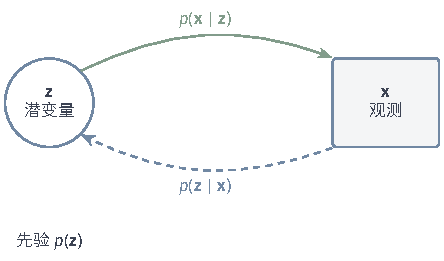
\includegraphics[width=75.188mm]{figures/04-classic-models/00-shared/tikz/dim-latent-model/figure.pdf}
  \caption{概率生成与后验推断的结构示意。实线表示$\bm{z}\to\bm{x}$的生成方向；虚线表示$\bm{x}\to\bm{z}$的后验推断，不是额外的生成依赖。图中节点与箭头只说明变量角色和条件关系，不表示实测数据、网络层数或计算流程；噪声描述观测对信号的偏离，不是新增的潜变量维数。}
\label{fig:dim-latent-model}
\end{figure}

独立高斯量线性组合仍为高斯量，将潜变量积分后得到
\begin{equation}
\label{eq:dim-ppca-marginal}
\begin{aligned}
p(\bm{x})&=\mathcal{N}(\bm{x};\bm{\mu},\bm{C}),\\
\bm{C}&=\bm{W}\bm{W}^\top+\sigma^2\bm{I}_d.
\end{aligned}
\end{equation}
信号协方差的秩至多为$k$，正噪声使$\bm{C}$正定；样本不足导致经验协方差奇异时，模型协方差仍可正定。

FA将噪声改为$\bm{\Psi}=\operatorname{diag}(\psi_1,\ldots,\psi_d)$，其中$\psi_j>0$为方差，故$\bm{C}=\bm{W}\bm{W}^\top+\bm{\Psi}$。给定因子，各维条件独立，跨维协方差由共同因子产生。独特方差也可包含特征自身的变化，解释时需结合测量机制；标准化会同时改变同方差假设的含义。

图\ref{fig:dim-ppca-fa-noise}固定载荷，只比较条件噪声。给定一个潜变量值，PPCA允许观测沿各方向等幅偏离均值，FA允许沿某坐标偏离更多。圆与椭圆均表示条件噪声；再混合不同潜变量值，才会加入信号协方差并形成总体分布。

\begin{figure}[htbp]
  \centering
  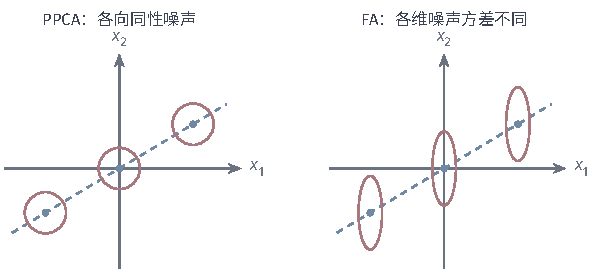
\includegraphics[width=101.840mm]{figures/04-classic-models/00-shared/tikz/dim-ppca-fa-noise/figure.pdf}
  \caption{PPCA与FA的条件噪声示意。设$d=2$、$k=1$、$\bm{\mu}=\bm{0}$、$\bm{W}=(1,0.6)^\top$，三个实心点对应$z=-1,0,1$的条件均值。左图取$\sigma=0.28$，右图取$\bm{\Psi}=\operatorname{diag}(0.16^2,0.50^2)$；每条轮廓到其中心的平方Mahalanobis距离均为$1$。坐标为无量纲构造值，轮廓是条件等密度线，不是总体数据云或置信区域。}
  \label{fig:dim-ppca-fa-noise}
\end{figure}

载荷的正交旋转$\bm{W}\bm{R}$不改变协方差。载荷满列秩且除旋转外局部可识别时，可扣除$k(k-1)/2$个旋转自由度：PPCA与FA的协方差参数数目分别为$dk+1-k(k-1)/2$及$dk+d-k(k-1)/2$，均值另有$d$个。FA还需排除载荷与噪声间的额外歧义。相较自由协方差的$d(d+1)/2$个参数，低秩约束可以降低估计方差，也可能带来模型偏差。

\subsubsection{参数学习}
\label{sec:dim-ppca-learning}

设样本独立同分布，均值为$\bar{\bm{x}}$，中心化量为$\bm{y}_i=\bm{x}_i-\bar{\bm{x}}$，记$\bm{S}=n^{-1}\sum_i\bm{y}_i\bm{y}_i^\top$。固定$\bm{C}$时，均值梯度$n\bm{C}^{-1}(\bar{\bm{x}}-\bm{\mu})$与负定二阶导数给出$\hat{\bm{\mu}}=\bar{\bm{x}}$。代回最大似然目标得
\begin{equation}
\label{eq:dim-ppca-likelihood}
\ell=-\frac{n}{2}\left[
d\log(2\pi)+\log|\bm{C}|
+\operatorname{tr}(\bm{C}^{-1}\bm{S})\right].
\end{equation}
对数行列式惩罚过大的协方差体积，迹项则惩罚在数据有较大变化的方向上赋予过小方差。

对$\bm{S}$作谱分解$\bm{U}\bm{\Lambda}\bm{U}^\top$，按$\lambda_1\geq\cdots\geq\lambda_d\geq0$排列。令$\bm{U}_k$包含前$k$个方向，$\bm{\Lambda}_k=\operatorname{diag}(\lambda_1,\ldots,\lambda_k)$。

证明需要比较两组谱的配对。Birkhoff--von Neumann分解说明：行和、列和均为$1$的非负方阵，即双随机矩阵，可以写成置换矩阵的凸组合\scite{birkhoff1946}因此双随机矩阵上的线性目标至少为某个置换取值的最小值。

最大似然解以PCA主方向构造载荷，以舍弃特征值的均值估计噪声，载荷内部保留旋转自由。下面先证明样本谱与模型谱同序配对最优，再优化谱值，从而说明全局最优性；奇异点及高维统计保证仍需另外讨论。

\begin{theorem}[PPCA最大似然解的存在条件与闭式表示]
\label{thm:dim-ppca-mle}
设$1\leq k<d$，尾谱均值$\tau=(d-k)^{-1}\sum_{j=k+1}^d\lambda_j$满足$\tau>0$且$\lambda_k>\tau$。在$\sigma^2>0$的PPCA模型中，以下参数达到全局最大似然：
\begin{equation}
\label{eq:dim-ppca-mle}
\begin{aligned}
\hat{\bm{\mu}}&=\bar{\bm{x}},\qquad
\hat{\sigma}^2=\tau,\\
\hat{\bm{W}}&=\bm{U}_k(\bm{\Lambda}_k-\tau\bm{I}_k)^{1/2}\bm{R}.
\end{aligned}
\end{equation}
其中$\bm{R}$为任意$k$阶正交矩阵。截断处有重根时，$\bm{U}_k$可在对应特征子空间内选取不同正交方向。
\end{theorem}

\begin{proof}
需最小化$F(\bm{C})=\log|\bm{C}|+\operatorname{tr}(\bm{C}^{-1}\bm{S})$。写$s=\sigma^2$，由信号半正定且秩至多为$k$，可行协方差的谱满足
\[
c_1\geq\cdots\geq c_k\geq s,\qquad
c_{k+1}=\cdots=c_d=s>0.
\]
允许$c_j=s$便包括载荷秩不足$k$的情况。

固定谱，设$\bm{p}_b$为$\bm{C}$的第$b$个单位特征向量，则
\[
\operatorname{tr}(\bm{C}^{-1}\bm{S})
=\sum_{a=1}^d\sum_{b=1}^d
\frac{\lambda_a}{c_b}(\bm{u}_a^\top\bm{p}_b)^2.
\]
平方内积构成非负且各行各列和为$1$的双随机矩阵，可写成置换矩阵的凸组合，所以上式不小于置换配对的最小值。若$\lambda_a\geq\lambda_b$、$c_a\geq c_b$，同序配对减去交换配对等于
\[
(\lambda_a-\lambda_b)
\left(\frac{1}{c_a}-\frac{1}{c_b}\right)\leq0.
\]
消去逆序配对即得$\operatorname{tr}(\bm{C}^{-1}\bm{S})\geq\sum_j\lambda_j/c_j$，取$\bm{p}_j=\bm{u}_j$达到等号。对数行列式只依赖谱，故同序对齐是固定谱下的全局最优。

对齐后，目标化为
\[
\begin{aligned}
F&=\sum_{j=1}^k\left(\log c_j+\frac{\lambda_j}{c_j}\right)\\
&\quad+(d-k)\log s+\frac{(d-k)\tau}{s}.
\end{aligned}
\]
暂去$c_j\geq s$及排序约束。对$a>0$，函数$g_a(v)=\log v+a/v$的导数为$(v-a)/v^2$，在$a$左侧为负、右侧为正，故$v=a$为唯一全局最小点。各首部项因此在$c_j=\lambda_j$处最小，尾部$(d-k)g_\tau(s)$在$s=\tau$处最小。

由$\lambda_k>\tau>0$，此解满足原约束。式~\eqref{eq:dim-ppca-mle}构造的协方差恰与$\bm{S}$同序对齐，首$k$个特征值为$\lambda_j$，其余为$\tau$，达到上述共同下界，故是全局最优。正交$\bm{R}$不改变载荷乘积；重根配对差为零，允许所述的不唯一性。
\end{proof}

边界情形要区分处理。$\lambda_k=\tau>0$时，同一公式仍给出最优协方差，但载荷降秩，满秩自由度与常规渐近分析不再直接适用。$\tau=0$时，样本协方差秩至多为$k$，未占据方向的方差可趋零使似然无界，正噪声模型中没有有限极大值。零噪声高斯分布奇异，已没有$d$维普通密度。

PPCA与PCA联系在主子空间，编码坐标还要由后验确定。生成模型的联合分布为
\begin{equation}
\label{eq:dim-ppca-joint}
\begin{bmatrix}\bm{z}\\ \bm{x}\end{bmatrix}
\sim\mathcal{N}\left(
\begin{bmatrix}\bm{0}\\ \bm{\mu}\end{bmatrix},
\begin{bmatrix}
\bm{I}_k&\bm{W}^\top\\
\bm{W}&\bm{C}
\end{bmatrix}\right).
\end{equation}
高斯条件公式给出后验均值$\bm{W}^\top\bm{C}^{-1}(\bm{x}-\bm{\mu})$与协方差$\bm{I}_k-\bm{W}^\top\bm{C}^{-1}\bm{W}$。记$\bm{M}=\bm{W}^\top\bm{W}+\sigma^2\bm{I}_k$，由$\bm{C}\bm{W}=\bm{W}\bm{M}$得到$\bm{W}^\top\bm{C}^{-1}=\bm{M}^{-1}\bm{W}^\top$，于是
\[
\bm{I}_k-\bm{M}^{-1}\bm{W}^\top\bm{W}
=\sigma^2\bm{M}^{-1}.
\]
将两项合并，后验写为
\begin{equation}
\label{eq:dim-ppca-posterior}
p(\bm{z}\mid\bm{x})
=\mathcal{N}\left(
\bm{M}^{-1}\bm{W}^\top(\bm{x}-\bm{\mu}),
\sigma^2\bm{M}^{-1}\right).
\end{equation}
即使参数已知，正噪声下的因子后验也仍有非零方差。后验均值编码给出一个点估计，却不能确定每个观测背后唯一的真实潜变量。
在最大似然解中取$\bm{R}=\bm{I}_k$，后验均值的第$j$个坐标为
\begin{equation}
\label{eq:dim-ppca-score}
\mathbb{E}[z_j\mid\bm{x}]
=\frac{\sqrt{\lambda_j-\tau}}{\lambda_j}
\bm{u}_j^\top(\bm{x}-\bar{\bm{x}}).
\end{equation}
该坐标是PCA得分的缩放。再映回观测空间时，第$j$方向的系数为$1-\tau/\lambda_j$，而正交投影的系数为$1$。教学谱$(9,1,1)$取$k=1$，有$\tau=1$、载荷$\sqrt8\bm{u}_1$、后验方差$1/9$及重构系数$8/9$。

线性同方差假设使后验协方差不随完整观测值改变，它也未计入参数估计误差。固定满列秩载荷、令噪声趋零时，重构趋向列空间正交投影，潜在坐标仍受载荷尺度影响。

FA通常用迭代估计。\term{期望最大化}（expectation-maximization, EM）在E步求潜变量后验矩，在M步最大化完全数据对数似然的后验期望\scite{clust-dempster1977}“完全数据”包含观测与潜变量，是似然构造的对象，未表示潜变量已经测得。

各维均已观测时，可固定$\bm{\mu}=\bar{\bm{x}}$。第$t$轮E步计算
\begin{equation}
\label{eq:dim-fa-estep}
\begin{aligned}
\bm{V}^{(t)}
&=\left[\bm{I}_k+
(\bm{W}^{(t)})^\top(\bm{\Psi}^{(t)})^{-1}
\bm{W}^{(t)}\right]^{-1},\\
\bm{m}_i^{(t)}
&=\bm{V}^{(t)}(\bm{W}^{(t)})^\top
(\bm{\Psi}^{(t)})^{-1}\bm{y}_i,\\
\bm{Q}_i^{(t)}
&=\bm{V}^{(t)}+\bm{m}_i^{(t)}(\bm{m}_i^{(t)})^\top.
\end{aligned}
\end{equation}
$\bm{m}_i^{(t)}$、$\bm{V}^{(t)}$与$\bm{Q}_i^{(t)}$分别为均值、协方差与二阶矩。将它们汇总为
\[
\bm{A}^{(t)}=\frac1n\sum_i\bm{y}_i(\bm{m}_i^{(t)})^\top,
\qquad
\bm{B}^{(t)}=\frac1n\sum_i\bm{Q}_i^{(t)}.
\]
M步由这些统计量更新载荷及噪声：
\begin{equation}
\label{eq:dim-fa-mstep}
\begin{aligned}
\bm{W}^{(t+1)}&=\bm{A}^{(t)}(\bm{B}^{(t)})^{-1},\\
\bm{\Psi}^{(t+1)}
&=\operatorname{diag}\left[
\bm{S}-\bm{W}^{(t+1)}(\bm{A}^{(t)})^\top
\right].
\end{aligned}
\end{equation}
$\operatorname{diag}$保留对角元。将载荷正规方程代入期望残差协方差，就得到噪声更新，实际只需$\bm{S}$的对角。二阶矩必须包含后验协方差$\bm{V}^{(t)}$，否则会低估噪声。PPCA的EM则对各维残差方差再取平均。

可用PPCA载荷及正对角残差初始化，再交替两步。对角逆用除法，其他逆由线性方程求解。若约束$\psi_j\geq\varepsilon>0$并将更新截到下界，应明确这是受约束估计。停止诊断可用
\begin{equation}
\label{eq:dim-fa-stopping}
\begin{aligned}
r_\ell^{(t)}
&=\frac{|\ell^{(t+1)}-\ell^{(t)}|}{1+|\ell^{(t)}|},\\
r_C^{(t)}
&=\frac{\lVert\bm{C}^{(t+1)}-\bm{C}^{(t)}\rVert_{\mathrm{F}}}
{1+\lVert\bm{C}^{(t)}\rVert_{\mathrm{F}}}.
\end{aligned}
\end{equation}
两项残差连续若干步低于容差时停止，并设置最大轮数。协方差残差不受载荷旋转影响，达到轮数上限却仅表示预算耗尽。

\subsubsection{理论分析}
\label{sec:dim-ppca-analysis}

\paragraph{表达能力}
PPCA能精确表达的观测分布是均值任意、协方差为$\bm W\bm W^\top+\sigma^2\bm I_d$的高斯分布。给定真实高斯协方差$\bm C_\star$，存在这样的表示，当且仅当能选$\sigma^2>0$，使$\bm C_\star-\sigma^2\bm I_d$半正定且秩至多为$k$。必要性来自信号协方差，充分性则由这个半正定矩阵的谱平方根构造$\bm W$。这意味着至多$k$个方向可在共同噪声方差之上再增加变化；剩余方向必须有相同方差。异质传感器噪声不满足这一条件时，PPCA即使优化充分，也只能用受限协方差近似它。

FA将条件改成存在正对角$\bm\Psi$，使$\bm C_\star-\bm\Psi$半正定且秩至多为$k$，因而可以精确表达由$k$个高斯共同因素及各坐标独立高斯扰动生成的数据。它扩大了噪声范围，跨坐标协方差仍必须由有限个共同因素产生。两种模型的边缘分布都是单个高斯；即使均值和协方差完全匹配，一个具有不同峰或非高斯尾部的真实分布也未必被精确表达。正噪声还使观测分布充满整个空间，低维的是信号而非每个带噪观测。

恢复真实因子是另一项限制。正交旋转$\bm W\bm R$保持观测分布不变，FA中信号对角方差与独特方差还可能有额外歧义；精确拟合观测密度不等于辨认唯一的物理因素。

\paragraph{收敛性}

条件满足时，PPCA谱解达到全局最大似然。FA的精确EM提高当前似然的相切下界，使似然不下降；有上界时似然值收敛。参数趋近驻点还需连续性与迭代有界等条件，全局最优仍无保证。弱因子与近零独特方差可能使更新缓慢。

\paragraph{泛化性}
PPCA与FA都给出观测密度，新样本的对数损失因此是与训练最大似然对应的风险。载荷可以旋转而不改变密度，直接比较风险也省去了为参数一致性选择唯一载荷的步骤。

\begin{theorem}[PPCA与因子分析在非退化有界参数下的期望对数风险界]
 \label{thm:dim-ppca-fa-risk}
设$D_n$独立同分布于$P$，$\lVert\bm X\rVert_2\leq r$几乎处处。训练前固定潜维数$k$，限制均值$\lVert\bm\mu\rVert_2\leq A$，并要求观测协方差
$\bm C=\bm W\bm W^\top+\bm\Psi$满足
$a\bm I\preceq\bm C\preceq b\bm I$，其中$0<a\leq b$。
PPCA保留$\bm\Psi=\sigma^2\bm I$，FA保留正对角$\bm\Psi$；两种协方差结构分别组成候选集$\Theta_k$。$P$不必属于这些高斯族。
定义$R(\bm\mu,\bm C)=\mathbb E_P[-\log\mathcal N(\bm X;\bm\mu,\bm C)]$，将经验平均对数损失距$\Theta_k$内全局最优的差记为$e_n$。令
\[
 \begin{aligned}
 p_0&=d+d(d+1)/2,& B_0&=\sqrt{A^2+db^2},\\
 M_0&=\tfrac d2\log(b/a)+\tfrac{(r+A)^2}{2a},\\
 L_0^2&=\frac{(r+A)^2}{a^2}
      +\frac14\left(\frac{(r+A)^2}{a^2}+\frac{\sqrt d}{a}\right)^2.
 \end{aligned}
\]
这些常数分别控制均值--协方差参数的维数与半径、对数损失区间和参数扰动。协方差下界保证逆矩阵与损失有界，上界及均值限制保证候选集的有限覆盖。与GMM相同的高斯密度的导数计算，配合引理\ref{thm:clustering-cover-risk}，对两种学习器均给出
\begin{equation}
 \begin{aligned}
 \mathbb E_{D_n}R(\widehat{\bm\mu},\widehat{\bm C})
 &\leq\inf_{(\bm\mu,\bm C)\in\Theta_k}R(\bm\mu,\bm C)\\
 &\quad+\frac{4L_0B_0}n
       +2M_0\sqrt{\frac{p_0\log(1+2n)+\log2}{2n}}\\
 &\quad+\mathbb E_{D_n}e_n.
 \end{aligned}
 \label{eq:dim-ppca-fa-risk}
\end{equation}
\end{theorem}

概率至少为$1-\delta$的版本将$\log2$换成$\log(2/\delta)$。本界使用完整协方差族的覆盖数，因此对PPCA和FA都是有效但保守的上界；它没有利用低秩结构获得更小的维数常数。若真实密度有有限熵，减去熵后就是相对该候选族最佳高斯密度的KL风险界。

训练均值与协方差估计使经验对数损失接近总体对数损失，受约束经验优化再把这一偏差转成所选密度的超额风险。精确求解使$e_n=0$，FA的局部EM解保留这一项。前述PPCA谱公式解决原最大似然问题；加入这里的边界约束后，需确认谱解仍可行或重新求解受约束目标。参数渐近正态性及Fisher信息描述另外的估计问题，不能直接代替这个新样本风险结论。

维数$k$也需选择。常规正则模型可比较
$\mathrm{AIC}=-2\hat\ell+2p$与$\mathrm{BIC}=-2\hat\ell+p\log n$，$p$为均值与可识别协方差的参数数目；奇异点需其他证据近似或独立验证。这些准则本身没有给出式\eqref{eq:dim-ppca-fa-risk}中的有限样本保证。所选$k$受噪声及用途影响，未必等于内在维数$m$。

若样本$i$只观测坐标集$O_i$，其似然使用已观测子向量的边际分布：
\begin{equation}
\label{eq:dim-linear-missing}
\bm{x}_{i,O_i}\sim
\mathcal{N}(\bm{\mu}_{O_i},\bm{C}_{O_i,O_i}).
\end{equation}
训练将各样本的边缘对数似然相加。E步只用$\bm{W}_{O_i,:}$与$\bm{\Psi}_{O_i,O_i}$，后验协方差随观测模式改变。M步按实际观测更新各维，或将缺失值和潜变量一并作为未观测量，求必要的一、二阶矩。

补全可用高斯条件均值，同时保留条件协方差或作条件采样以传播不确定性。若只填均值并视作真实观测，后续分析会低估误差。

忽略缺失机制通常需要\term{随机缺失}（missing at random, MAR）：给定已观测值，缺失概率不再依赖未观测值，且机制参数与数据参数可独立取值。若指标越严重越容易未被记录，仅用观测边缘似然仍可能有偏，需模型化缺失机制\scite{rubin1976missing}

概率模型把补全、表示与似然统一起来，PCA也可以构造其他补全方案。多个局部线性结构可进一步组成混合PPCA，其识别与退化需另查。

\subsubsection{优化表达能力}

\paragraph{组合多个局部线性分布}
一个全局线性子空间难以重构圆周，较短的圆弧却可以分别近似为直线。Tipping与Bishop的\term{混合PPCA}（mixture of PPCA）采用多个局部线性模型，以非负且和为$1$的权重混合它们的密度\scite{tipping1999mixture}。像高斯混合模型一样，它引入成分变量和责任度，每个成分又有低秩信号及噪声。EM共同估计责任度与载荷，联系软聚类和局部降维（参见第\ref{sec:clustering-gmm}节）。多个局部模型并不自动拼成连续坐标，局部坐标间的衔接、分量坍缩与零噪声退化仍需处理。它能精确表达的是有限个受PPCA协方差约束的高斯密度的混合。更多成分允许覆盖更多局部线性区域，却没有使固定成分数的模型自动精确拟合任意弯曲分布。

\paragraph{表示非高斯观测分布}
PPCA用高斯噪声解释重构误差，计数或二值观测则有不同取值范围和波动规律。\term{指数族PCA}对分布的自然参数施加低秩结构，以条件似然取代平方损失：计数可用泊松分布，二值可用伯努利分布，正连续数据可用满足参数域的Gamma观测。它把前文GLM的观测分布选择带入低秩表示。Collins、Dasgupta与Schapire的推广未必设置潜变量先验，因此还需区分低秩分解和完整生成模型\scite{collins2001exponential}。精确表达要求真实条件分布属于所选指数族，且其自然参数矩阵满足指定的低秩约束。均值是自然参数的非线性函数，所以自然参数低秩不等于观测均值低秩；例如低秩Logit经Sigmoid变换后，一般不再是同秩矩阵。

\subsubsection{优化泛化能力}

潜在方向需要保留多少，也可以交给带先验的估计。Bishop的\term{贝叶斯PPCA}给载荷列加分层先验，例如$\bm{W}_{:,r}\mid\beta_r\sim\mathcal{N}(\bm{0},\beta_r^{-1}\bm{I}_d)$，其中$\beta_r>0$。数据若不足以支持某一方向，较大的$\beta_r$会把该列载荷压向零，按各列的收缩程度调整实际使用的复杂度\scite{bishop1999bayesian}。算法也可采用证据最大化，把离散的维数比较转为超参数估计，同时增加先验选择与近似推断的成本。所选复杂度受模型与推断影响，并不保证恢复真实维数。给载荷加先验没有扩大固定参数下的线性高斯协方差族；对参数积分可以增加预测分布的不确定性，但仍须区分后验预测与已知参数时的观测模型。

\subsubsection{小结}
\label{sec:dim-ppca-summary}

PPCA与FA用线性潜在因素解释共同变化，分别采用同方差与特征特异噪声。高斯条件推断可以组织编码与缺失值处理，前提是噪声及缺失机制与观测相符。模型选择需同时考虑潜在维数、测量误差和实际编码用途。

一个全局子空间不足时，混合PPCA使用多个局部成分，同时增加责任度、成分数及坐标衔接的处理。维数不明确时，载荷先验让复杂度参与估计，同时增加先验和推断选择。计数或二值输入则需要改变观测分布，自然参数上的低秩结构也要按相应含义解释。这些扩展分别回应几何、复杂度与取值机制，不能仅凭都采用潜变量就混用假设。

\subsection{高斯过程潜变量模型（GPLVM）}
\label{sec:dim-gplvm}

概率PCA和因子分析都用线性映射把潜在状态转成观测，少量状态控制的变化却未必沿直线展开。一个简单的构造例子是转动角度$z$生成观测$(\cos z,\sin z)$：潜在状态只有一维，观测却沿圆周变化，一维线性生成模型的无噪声信号只能沿一条直线变化。\term{高斯过程潜变量模型}（Gaussian process latent variable model, GPLVM）为低维状态到各观测坐标的函数设置GP先验，用核规定允许的非线性变化，再从观测反求未知状态坐标。它与高斯过程回归共享核协方差及边缘似然计算；回归输入已知，本节输入也是待估计量（参见第\ref{sec:regression-gpr}节）。

Lawrence于2003年提出GPLVM，2005年系统论述其模型\scite{lawrence2005gplvm}。推导从概率PCA的对偶表述出发，将载荷积分掉、转而估计潜在坐标，再以GP引入非线性函数先验。映射的不确定性被积分，坐标仍可作点估计，两者处理方式由此不同。

\subsubsection{模型结构}
\label{sec:dim-gplvm-structure}

\term{高斯过程}（Gaussian process, GP）规定有限输入处的函数值联合为高斯，核控制相关性与变化尺度。这里$\bm{X}$按训练均值中心化，生成时加回均值，$\bm{Z}\in\mathbb{R}^{n\times k}$按行存坐标。设
\begin{equation}
\label{eq:dim-gplvm-generative}
\begin{aligned}
f_j&\sim\mathcal{GP}(0,\kappa_{\bm{\theta}}),
\qquad j=1,\ldots,d,\\
x_{i,j}&=f_j(\bm{z}_i)+\epsilon_{i,j},
\qquad \epsilon_{i,j}\sim\mathcal{N}(0,\sigma^2).
\end{aligned}
\end{equation}
各输出函数独立并共享核参数$\bm{\theta}$，同一函数跨样本的值由核相关。噪声相互独立且独立于函数。非参数先验未预先限定固定有限基函数，核与噪声仍有待学习参数。

固定坐标并积分函数值。定义$\bm{K}_{i,h}=\kappa_{\bm{\theta}}(\bm{z}_i,\bm{z}_h)$及$\bm{C}_Z=\bm{K}+\sigma^2\bm{I}_n$，得到
\begin{equation}
\label{eq:dim-gplvm-likelihood}
\begin{aligned}
p(\bm{X}\mid\bm{Z})
&=\prod_{j=1}^d
\mathcal{N}(\bm{X}_{:,j};\bm{0},\bm{C}_Z),\\
\ell&=-\frac{nd}{2}\log(2\pi)
-\frac{d}{2}\log|\bm{C}_Z|\\
&\quad-\frac{1}{2}
\operatorname{tr}(\bm{C}_Z^{-1}\bm{X}\bm{X}^\top).
\end{aligned}
\end{equation}
$\bm{C}_Z$跨样本，为$n$阶；PPCA的协方差则跨观测维，为$d$阶。基本GPLVM优化$\bm{Z},\bm{\theta},\sigma^2$，保留坐标点估计。加独立标准高斯坐标先验后，目标多出$-\lVert\bm{Z}\rVert_{\mathrm{F}}^2/2$，最大后验估计仍只取坐标的一个值。

线性核$\kappa(\bm{z},\bm{z}')=\bm{z}^\top\bm{z}'$对应标准高斯载荷的线性函数先验。积分载荷并估计坐标，得到$\bm{C}_Z=\bm{Z}\bm{Z}^\top+\sigma^2\bm{I}_n$，称为\term{对偶PPCA}。它与PPCA交换积分和估计的对象，联合模型也随之改变。

对$\bm{G}=\bm{X}\bm{X}^\top/d$作谱分解，记有序特征值为$\rho_i$，前$k$个特征向量为$\bm{V}_k$，$\bm{D}_k=\operatorname{diag}(\rho_1,\ldots,\rho_k)$。无坐标先验惩罚，且$k<n$、$\eta=(n-k)^{-1}\sum_{i>k}\rho_i>0$、$\rho_k>\eta$时，同一谱证明给出
\begin{equation}
\label{eq:dim-gplvm-dual}
\begin{aligned}
\hat{\sigma}_{\mathrm{dual}}^2&=\eta,\\
\hat{\bm{Z}}&=\bm{V}_k(\bm{D}_k-\eta\bm{I}_k)^{1/2}\bm{R}.
\end{aligned}
\end{equation}
这里按$d$归一化，而PPCA按$n$归一化。左右奇异向量将两者联系到PCA，缩放、噪声估计及条件分布却不同。坐标先验改变目标后，也需重新求解。

平方指数、Matérn等核允许非线性生成，并规定相应平滑性。核选择限制可表达的函数。核PCA在已知观测上计算核，GPLVM在待学习坐标上计算核，二者核化的对象不同。

\subsubsection{参数学习}
\label{sec:dim-gplvm-learning}

在固定互异潜在坐标上，严格正定核的有限协方差为正定，函数值先验便在全部有限观测值邻域上赋予正概率；这只说明有限数据可以被拟合，未说明学得了真实流形或正确的样本外映射。

坐标目标非凸，可用PCA初始化后，以L-BFGS或共轭梯度优化负对数似然。比较多次初始化时，固定训练划分与优化预算，考察最终对数似然。部分核有平移、旋转或坐标尺度与长度尺度的补偿对称，坐标解因而可能不唯一。

样本外检验时固定训练模型，遮住新样本的部分观测坐标，仅用其余坐标反求潜在位置，再计算被遮坐标的平均条件预测对数密度；值越大表示模型对这些未用于编码的观测赋予的密度越高。

微分行列式与逆矩阵，先得协方差梯度，再用链式法则传到参数：
\begin{equation}
\label{eq:dim-gplvm-gradient}
\begin{aligned}
\bm{H}&:=\frac{\partial\ell}{\partial\bm{C}_Z}\\
&=\frac12\bm{C}_Z^{-1}\bm{X}\bm{X}^\top\bm{C}_Z^{-1}
-\frac d2\bm{C}_Z^{-1},\\
\frac{\partial\ell}{\partial a}
&=\operatorname{tr}\left(
\bm{H}^\top\frac{\partial\bm{C}_Z}{\partial a}\right).
\end{aligned}
\end{equation}
$a$可表示坐标、核超参数或噪声方差，第二式将似然梯度传到具体未知量。

一个坐标同时改变核矩阵的行与列，求导需计入两者；正参数可在对数空间优化。

用Cholesky分解$\bm{C}_Z=\bm{L}\bm{L}^\top$代替显式求逆，以$2\sum_i\log L_{i,i}$计算对数行列式，用三角求解计算逆的作用。数值抖动用于稳定求解，应与统计噪声分别记录。

每轮更新潜在坐标后都要处理核矩阵，稠密GPLVM需要$O(n^3)$时间及$O(n^2)$存储。

给定潜在坐标，GP条件分布可以预测观测，方差含函数不确定性与观测噪声。给定新观测要编码时，坐标仍未知，需要反求
\begin{equation}
\label{eq:dim-gplvm-encoding}
\hat{\bm{z}}_*=\argmax_{\bm{z}}
\left\{\log p(\bm{x}_*\mid\bm{z},\bm{X},\bm{Z})
+\log p(\bm{z})\right\},
\end{equation}
无先验版本删去先验项。反问题可能多解，需初始化或近似坐标后验。有噪声时，位置后验还可能重叠。正向GP预测本身未给出直接编码器，学习反向映射属于额外扩展。

输出$j$只在$I_j$处观测时，用$\mathcal{N}(\bm{X}_{I_j,j};\bm{0},(\bm{C}_Z)_{I_j,I_j})$计算似然。各输出缺失模式不同，就不能共用一次完整分解。给定坐标可预测缺失值，但尚未传播坐标不确定性，仍需满足缺失可忽略条件。

\subsubsection{理论分析}
\label{sec:dim-gplvm-theory}

\paragraph{表达能力}
GPLVM把线性信号空间换成核允许的函数$\bm f:\mathbb R^k\to\mathbb R^d$的像。若真实无噪声观测确实由这样的$\bm f$及$k$维坐标生成，就不再要求所有观测落在一个线性子空间；例如一个允许相应周期变化的函数先验能够描述$(\cos z,\sin z)$的圆周。这里说的是生成函数的范围，核的平滑性与潜变量支持仍决定哪些曲线或曲面可被描述，并非任意核都能表示任意流形\scite{lawrence2005gplvm}。

正观测噪声使生成分布围绕函数像扩散，因此带噪记录一般不严格落在$k$维曲面上。若$\bm f$在潜变量支持上不是单射，不同潜在位置还可生成同一无噪声观测。对各向同性距离核，整体平移或旋转潜在坐标保持核矩阵不变；同时缩放坐标与核长度尺度也可能保留同一矩阵。这些对称性说明，即使观测拟合很好，潜在坐标的原点、朝向或单位仍不能仅由似然辨认。



\paragraph{收敛性}
若潜在坐标与核参数限制在紧致域内，且噪声方差有严格正的下界，核矩阵保持正定，负对数似然连续，因而存在最小值。去掉这些限制后，不能仅凭似然形式断言解存在或唯一；坐标平移、旋转等对称性已经给出非唯一情形。

对光滑核，在一个凸紧致参数域$\Theta$上令负对数似然为$F$，其梯度的Lipschitz常数为$L>0$。投影梯度步$\bm\theta^{(t+1)}=\Pi_\Theta(\bm\theta^{(t)}-\nabla F(\bm\theta^{(t)})/L)$满足
\[
 \min_{0\leq t<T}\lVert L(\bm\theta^{(t)}-\bm\theta^{(t+1)})\rVert_2^2
 \leq\frac{2L[F(\bm\theta^{(0)})-\min_\Theta F]}{T}.
\]
该式由每步至少下降$\tfrac L2\lVert\bm\theta^{(t+1)}-\bm\theta^{(t)}\rVert_2^2$并求和得到。它给出趋近一阶约束驻点的速度，不是全局目标差的速度，也不自动适用于前面列举的任意拟牛顿实现。稠密更新每步仍需承担核矩阵分解的成本。

\paragraph{泛化性}
GPLVM的训练似然涉及整批未知坐标与一个共享随机函数，不能当作固定点密度的$n$项独立同分布损失。提高这项联合似然或ELBO，并未直接界定独立新观测的对数风险。要评价预测密度，先固定训练后得到的GP预测分布及潜变量先验，并对潜变量积分：
\[
 q_j(\bm x)=\int p_j(\bm x\mid\bm z,D_n)
                    p_j(\bm z\mid D_n)\,\mathrm d\bm z.
\]
基本版本可预先指定潜变量先验，贝叶斯版本则使用所声明的后验预测制度。仅将新观测的最优潜在坐标代入条件似然，不一定得到积分为一的观测密度，不能替代$q_j$。

一个可直接成立的风险结论针对独立验证选出的预测器。

\begin{theorem}[GPLVM在预测密度有界与独立验证下的期望风险界]
 \label{thm:dim-gplvm-validation-risk}
取预定的置信参数$\delta\in(0,1)$。
条件于训练集及训练随机性，冻结$J$个候选密度$q_1,\ldots,q_J$。假设它们在$P$的支持上均满足$0<q_-\leq q_j(\bm x)\leq q_+<\infty$，令$M=\log(q_+/q_-)$。用独立于训练的$m$个独立同分布验证观测选择平均对数损失最小的$\widehat j$，允许验证求解误差$e_m$。则以至少$1-\delta$的验证抽样概率，
\begin{equation}
 \mathbb E_P[-\log q_{\widehat j}(\bm X)]
 \leq\min_{1\leq j\leq J}\mathbb E_P[-\log q_j(\bm X)]
     +2M\sqrt{\frac{\log(2J/\delta)}{2m}}+e_m.
 \label{eq:dim-gplvm-validation-risk}
\end{equation}
\end{theorem}

对冻结候选的验证损失作Hoeffding界与并集界，再用验证最优性承担两次偏差，就得到此式；验证抽样平均的版本将$\log(2J/\delta)$换成$\log(2J)$。条件于训练集的结论也可再对训练集取平均。

这里保证的是在已训练候选中的预测密度选择，未保证原GPLVM联合优化得到总体最佳生成模型。参数、坐标的求解与反向编码误差仍影响候选本身；密度上下界也是明确的附加条件。若任务改为缺失坐标预测，还需在相同缺失制度下定义条件损失并使用独立验证。

\subsubsection{优化泛化能力}

候选潜在维数较大时，并非每个坐标都需要参与观测生成。自动相关性确定（automatic relevance determination, ARD）为各潜在方向学习独立长度尺度。逆长度尺度平方$\alpha_r$控制该方向差异对相关性的作用。小$\alpha_r$表示核对该方向差异不敏感，可用于筛选有效方向。判断仍受先验、尺度、噪声及优化影响，也不能将筛选结果直接视为真维数。

\subsubsection{优化计算能力}

样本量较大时，稀疏GPLVM改用$b\ll n$个\term{诱导点}及其函数值概括训练信息，让许多观测通过这组较小的变量联系起来。核心矩阵计算由此降为$O(nb^2+b^3)$，输出与核计算另计；节省的计算以近似误差为代价\scite{lawrence2007sparse}。

\subsubsection{支持潜在位置后验估计场景}

基本GPLVM为每个样本选定一个潜在位置。观测噪声较大或部分坐标缺失时，多种位置都可能解释同一记录，只保留一个点就忽略了这部分不确定性。Titsias与Lawrence于2010年提出\term{贝叶斯GPLVM}\scite{titsias2010gplvm}。该模型用变分分布表示可能的坐标，再优化对数边缘似然的\term{证据下界}（evidence lower bound, ELBO）：
\begin{equation}
\label{eq:dim-gplvm-elbo}
\begin{aligned}
q(\bm{Z})&=\prod_i\mathcal{N}(\bm{z}_i;\bm{\nu}_i,\bm{S}_i),\\
\log p(\bm{X})&\geq\mathcal{L},\\
\mathcal{L}
&=\mathbb{E}_{q(\bm{Z})}[\log p(\bm{X}\mid\bm{Z})]\\
&\quad-\operatorname{KL}(q(\bm{Z})\Vert p(\bm{Z})).
\end{aligned}
\end{equation}
均值$\bm{\nu}_i$与正定协方差$\bm{S}_i$为变分参数，KL表示Kullback--Leibler散度。将边缘似然写为$q$下的期望，再用Jensen不等式将对数移入期望，得到上述下界：期望对数似然衡量观测拟合，KL惩罚近似后验偏离先验。等价地，
\[
  \log p(\bm{X})-\mathcal{L}
  =\operatorname{KL}\bigl(q(\bm{Z})\Vert p(\bm{Z}\mid\bm{X})\bigr)
  \geq0.
\]
下界不超过对数边缘似然，二者差距为近似与真实坐标后验的KL散度；只有两种后验一致，差距才为零。

随机核矩阵的逆与行列式使第一项仍难积分。原方法借助诱导函数值再构造可计算下界，使适当核与高斯变分分布所需的期望有解析式。诱导点位置、核参数及噪声通常继续作优化变量，尚未对全部未知量作贝叶斯积分。

可在同一留出规则下比较预测对数密度，并将后验预测区间在留出观测上的覆盖率与标称概率对照，检查变分模型的预测和不确定性估计。

\subsubsection{小结}
\label{sec:dim-gplvm-summary}

GPLVM把生成函数的输入也视为未知，借助GP函数先验描述潜在状态与观测之间的非线性关系。基本版本估计各样本的坐标，再作条件函数预测；给定新观测反求坐标却是另一个优化问题。姿态、运动或构象任务可以加入领域先验，核选择与局部求解仍影响学得的关系。

大样本的稠密核计算可用诱导点近似，节省矩阵计算同时引入近似误差。位置不确定时，贝叶斯GPLVM用变分分布代替单个坐标，增加了后验近似与下界优化。两者处理的是计算规模和坐标不确定性，新点的反向编码预算仍需另行安排。

\subsection{模型对比与总结}
\label{sec:dim-probabilistic-comparison}

概率降维先用生成机制解释观测变化，再从观测推断潜在状态。PPCA把所有观测坐标的剩余误差放在同一个噪声尺度下；传感器精度不同时，同方差假设就可能把部分测量误差吸收到共同信号中。FA保留线性潜在因素，改用各坐标自己的噪声方差，回应异质测量误差的问题，同时增加协方差分解的自由度和数值拟合。

噪声方差的调整没有改变线性生成关系。弯曲的观测变化需要多个局部线性成分，或一个允许非线性变化的共享函数。混合PPCA采用前一条路线，让成分责任度连接局部生成与软分组；GPLVM采用后一条路线，对潜在坐标到观测的函数设置GP先验。前者需要处理成分数和局部坐标衔接，后者需要选择核并联合求潜在坐标，二者并非只把同一个协方差估计器换成不同求解器。

潜变量不确定性又与函数不确定性不同。PPCA和FA在固定参数下可以计算线性高斯条件分布，基本GPLVM则为训练样本保留坐标点估计，并积分生成函数。贝叶斯GPLVM再用近似后验描述可能的坐标，增加下界求解和近似误差。表\ref{tab:dim-probabilistic-comparison}据此区分生成、学习和新观测编码，避免把GP预测方差直接当作潜在位置方差。

\begin{table*}[htbp]
\centering
\small
\begin{tabularx}{\linewidth}{@{}>{\RaggedRight\arraybackslash}p{20mm}>{\RaggedRight\arraybackslash}X>{\RaggedRight\arraybackslash}X>{\RaggedRight\arraybackslash}X@{}}
\toprule
比较方面 & PPCA & FA & GPLVM \\
\midrule
生成映射 & 线性，共享各向同性噪声 & 线性，各观测坐标独立噪声 & GP函数先验；非线性取决于核，基本噪声为同方差高斯 \\
学习方法 & 协方差谱分解或EM & EM或其他数值优化 & 优化坐标和超参数；贝叶斯版本优化变分下界 \\
潜变量不确定性 & 给定参数后的高斯条件推断 & 给定参数后的高斯条件推断 & 基本版本为坐标点估计；需后验近似才能量化位置不确定性 \\
新观测编码 & 一次线性变换 & 一次线性变换 & 通常需反求新坐标，GP正向预测本身不是编码 \\
缺失观测 & 观测子协方差边际化 & 观测子协方差边际化 & 按输出的观测索引选取核子矩阵 \\
主要用途 & 线性压缩、去噪、受约束协方差估计 & 异质测量误差、共同因子建模 & 非线性生成关系、给定潜变量的输出预测 \\
\bottomrule
\end{tabularx}
\caption{概率降维模型比较。后验以固定参数为条件；GPLVM的函数预测方差不是潜在坐标方差。缺失值处理均要求正确边际化及可忽略的缺失机制。}
\label{tab:dim-probabilistic-comparison}
\end{table*}

完整稠密数据下，PPCA构造协方差并完整分解约需$O(nd^2+d^3)$，截断SVD或EM另有成本。FA利用对角噪声，每轮约为$O(ndk+nk^2+dk^2+k^3)$，总成本再乘轮数$T$。稠密GPLVM每轮通常为$O(n^3+n^2d+n^2k)$。比较时应同时规定$n,d,k$和求解器。

\term{混合PPCA}（mixture of PPCA）以非负且和为$1$的权重混合多个局部PPCA密度\scite{tipping1999mixture}像高斯混合模型一样，它引入成分变量和责任度，每个成分又有低秩信号及噪声。EM共同估计责任度与载荷，联系软聚类和局部降维（参见第\ref{sec:clustering-gmm}节）。局部坐标间的连续性尚需额外构造，分量坍缩与零噪声退化也需控制。

\term{贝叶斯PPCA}可给载荷列加分层先验，例如$\bm{W}_{:,r}\mid\beta_r\sim\mathcal{N}(\bm{0},\beta_r^{-1}\bm{I}_d)$。较大$\beta_r$压缩载荷，以ARD调整复杂度\scite{bishop1999bayesian}算法也可采用证据最大化，所选复杂度受模型与推断影响，未保证恢复真实维数。

观测类型还决定适合的分布。\term{指数族PCA}约束自然参数的低秩结构，以条件似然取代平方损失。泊松适合计数，伯努利适合二值，正连续数据可用满足参数域的Gamma观测。Collins、Dasgupta与Schapire的推广未必设置潜变量先验，因此还需区分低秩分解和完整生成模型\scite{collins2001exponential}

谱分解、潜变量迭代与核矩阵计算需要不同预算。比较时应固定样本数、观测维数、潜在维数与求解器，并同时记录每轮成本和总轮数。

概率降维用生成假设解释误差，并组织编码与缺失值推断。线性信号可用PPCA或FA，非线性函数先验可用GPLVM；选择时要判断数据机制、预测目标及预算，并核对模型保留了哪些不确定性。

逐条反求坐标的成本也可以通过共享编码器处理。\term{变分自编码器}（variational autoencoder, VAE）用网络参数化生成分布与近似后验，以摊销推断复用编码计算\scite{kingma2013}。它同时改变生成函数族、后验近似与训练目标，属于另一类潜变量模型；相关神经表示入口参见\BookSectionRef{sec:neural-learned-representations}{卷五“模型：神经网络模型”的“从人工特征到可学习的表示”节}。共享编码减少逐条优化，仍需评价近似后验和生成模型的误差。

\Needspace{18\baselineskip}
\section{本章小结}
\label{sec:dim-summary}

降维需要以较少坐标保留当前用途所需的信息。PCA与核PCA按所选几何提取全局变化，距离法拟合点对差异，邻域法让局部关系约束坐标，概率法用低维因素解释观测生成。监督方向、稀疏约束、污染分解和非线性映射分别改变保留目标、允许的组合或观测假设，不能仅凭坐标更少或二维图更清楚判断调整是否合适。

内在维数$m$描述给定尺度、噪声和结构假设下的局部自由度，表示维数$k$是按任务选取的输出规模，显示维数$k_{\mathrm{vis}}\in\{2,3\}$只反映画图限制。应根据重构、距离、邻域或下游任务选择$k$，再检查核尺度、邻居数和初始化改变时，结论是否保持。邻域诊断还要区分新增的错误邻居与丢失的原有邻居，\term{信任度}（trustworthiness）检查低维新增邻居是否可信，\term{连续性}（continuity）检查原有邻居是否保留。这里“连续性”是邻域指标；二维图上的分组仍需在原表示中检验，并由任务信息解释其含义。

训练布局与共享编码回答不同问题。只有训练坐标时，结论针对这批对象；处理新记录还需要固定参考表示后的插值、定位或参数映射。直接矩阵编码、约束系数推断和逐点反求坐标也需要不同预算，应把表示与模型存储、编码与解码，以及训练的总迭代成本一起计算。

表示用于回归、分类或聚类时，均值、尺度、特征选择、核参数、字典及邻域图都应在训练划分内拟合，与后续模型共同验证，冻结规则后再用独立数据评价。预测用途可比较同一学习器使用原始输入、简单PCA与所选表示的结果；聚类用途还需在原特征或已验证表示中检查群组稳定性及外部证据。探索图形可以提出假设，保留了哪些关系及这些关系是否有用，仍由相应数据和指标回答。

\paragraph{扩展阅读}
进一步阅读可围绕生成解释与几何压缩的联系，比较同一表示在重构、邻域保留和预测任务中的作用，并核对所采用的噪声、映射与编码假设\scite{bishop2006,hastie2009}。

\chapter{集成学习}
\label{chap:ensemble-learning}

信用风险模型可能利用不同的预测信息：线性模型概括全局趋势，决策树表达局部交互；两棵树也可能因训练样本不同而作出不同判断。将这些预测组合起来，有机会减少单个模型遗漏结构或受训练波动影响造成的误差。\term{集成学习}（ensemble learning）研究成员模型的生成与输出组合，并分析成员之间的依赖如何影响新样本预测。

为了说明怎样组合预测，设训练集为
\[
  D_n=\{(\bm{x}_i,y_i)\}_{i=1}^{n},
\]
学习过程产生$M\geq1$个\term{成员模型}$h_1,\ldots,h_M$，每个成员都能对新输入给出一份预测。用$\mathcal{C}_{\bm{x}}$表示在当前输入处把这些预测合为一个输出的组合规则，得到\term{集成模型}
\begin{equation}
  H(\bm{x})
  =\mathcal{C}_{\bm{x}}\bigl(h_1(\bm{x}),\ldots,h_M(\bm{x})\bigr).
  \label{eq:ensemble-combination}
\end{equation}
组合规则可以固定，也可以根据输入调整成员权重；固定时省略下标$\bm{x}$。本章主要讨论监督预测。成员若都预测同一个回归目标，可以采用等权平均
\[
  H(\bm{x})=\frac{1}{M}\sum_{m=1}^{M}h_m(\bm{x}),
\]
也可以用非负权重$w_m$作加权平均，其中$\sum_m w_m=1$。分类成员则可能输出硬标签、类别得分或类别概率。硬标签对应类别投票，同尺度得分或同类概率可逐类平均后决策；混合不同输出前，需要把它们转换为含义一致的量。

组合之前需要明确输出的数值含义。直接平均不同尺度的分类得分，会使数值范围较大的成员占据更大作用；平均类别概率则保持概率向量形式，但它与真实类别频率是否对应仍需检验。回归均值、分位数和分布，以及分类标签、排序和概率各有评价对象，沿用前两章的区分。

组合能否减少预测错误，还取决于成员怎样产生。若各成员在同一区域都遗漏了同一关系，平均或投票仍会保留这一共同错误；若成员的错误发生在不同样本上，组合才有机会修正其中一部分。成员的预测能力与错误之间的依赖需要一起考虑，单纯增加成员数量并不保证风险下降。

围绕成员生成与组合的关系，本章介绍三类方法。Bagging让同一学习算法在不同重采样数据上分别训练，再平均或投票，主要处理训练样本扰动带来的预测波动。Boosting让新成员针对当前组合的不足训练，用一轮轮修正形成最终预测。Stacking则把已有成员的预测作为新输入，另外训练一个负责组合的模型；为避免这个模型学到成员对训练样本的过度拟合，需要使用未参与相应成员拟合的样本预测。三者分别改变训练数据、逐轮学习目标或组合规则，回答的是不同的改进问题。

图\ref{fig:ensemble-three-mechanisms}在同一预测任务中比较这三种训练依赖。给定原训练数据后，Bagging成员可分别训练；Boosting的新成员依赖前轮组合产生的修正信号；Stacking的组合层依赖成员在留出样本上的预测。依赖关系既决定哪些计算可以并行，也决定二阶段训练需要隔离哪些样本信息。

\begin{figure*}[htbp]
  \centering
  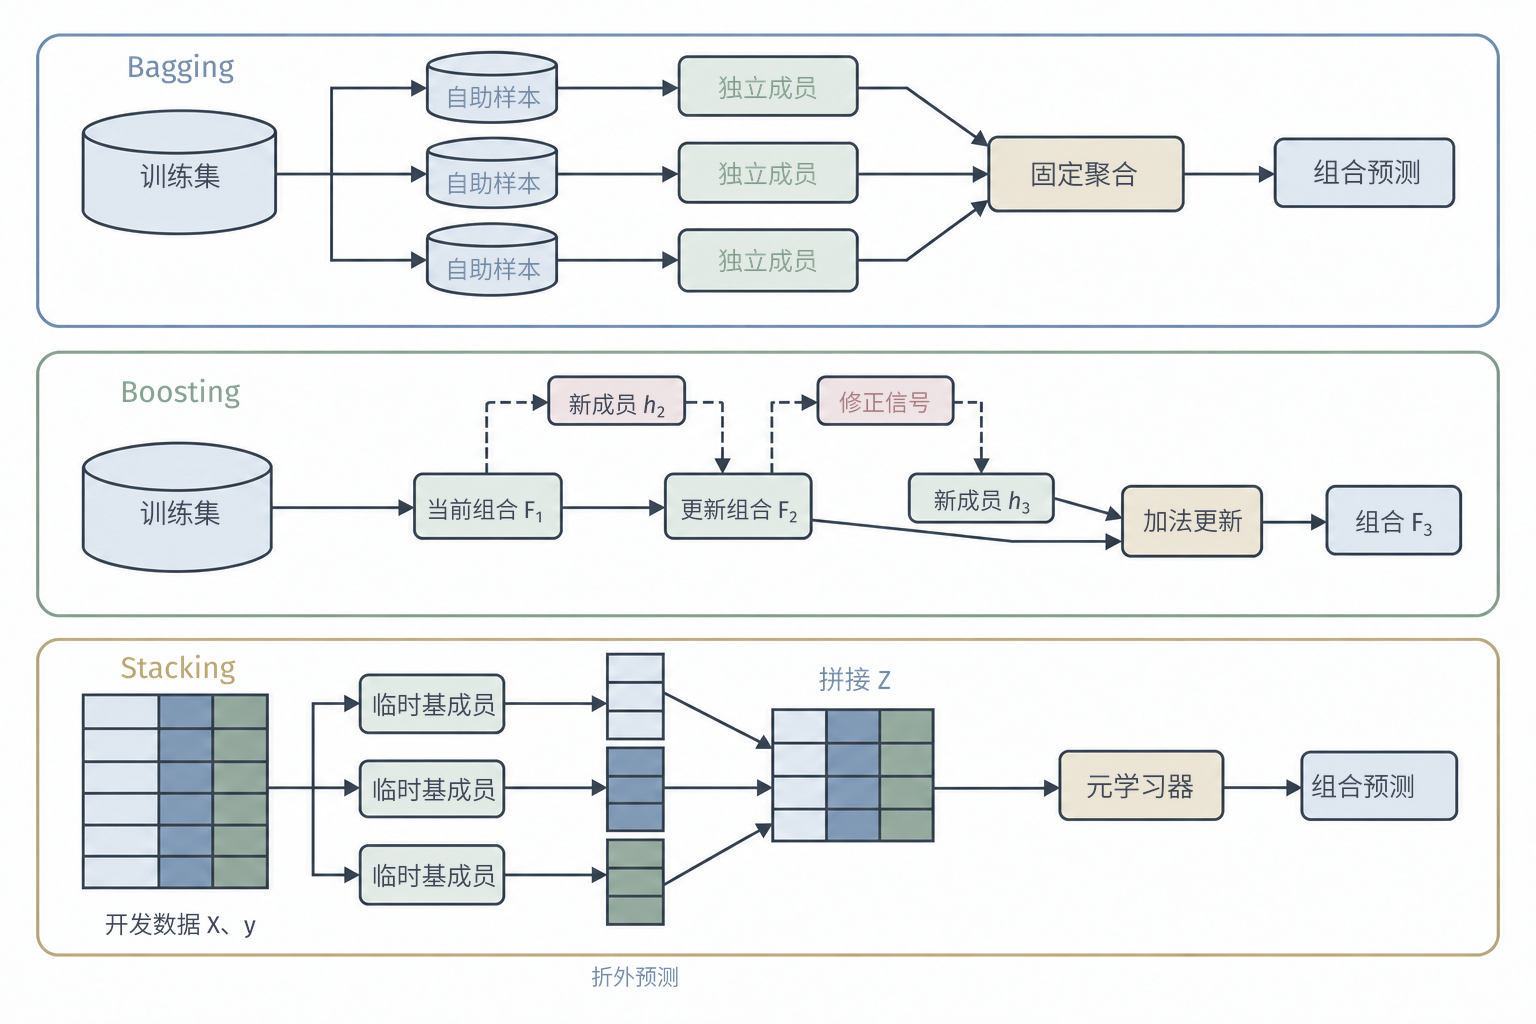
\includegraphics[width=130.048mm]{figures/04-classic-models/00-shared/generated/ensemble-three-mechanisms/figure.png}
  \caption{Bagging、Boosting与Stacking的成员生成及组合关系。实线连接训练与预测步骤，虚线传递当前组合形成的修正信号。三类机制的成员依赖及组合规则不同；示意流程允许采用不同成员模型。}
  \label{fig:ensemble-three-mechanisms}
\end{figure*}


\section{基于Bagging的集成}
\label{sec:ensemble-bagging}

单棵树的预测可能对训练样本很敏感。例如，根节点上两个候选分裂的得分很接近，替换少量训练记录就可能让另一分裂胜出；后续节点收到的样本随之改变，最终预测也可能不同。这正是上一节说的“方差大”。若能从同一总体反复抽取多份独立的训练集，分别建树后平均，各树因样本偶然性产生的波动就会相互抵消。困难在于现实中通常只有一份训练数据，不可能真的回到总体重新采样。

统计学的\emph{自助法}（bootstrap）提供了一个巧妙的替代：既然拿不到总体，就把手头这份样本当作总体的“缩影”，从中\emph{有放回地}重复抽样。具体做法是从$n$条记录里每次随机抽一条、记下后放回，连抽$n$次，得到一份同样大小的“自助样本”。由于是有放回抽取，同一条记录可能被抽中两三次，另一些记录则一次都没被抽中，于是每份自助样本都是原数据的一个略有不同的版本，模拟了“换一批数据”的效果。\term{装袋法}（bootstrap aggregating, Bagging）就是从现有训练集抽取多份自助样本，分别训练成员，再对数值预测取平均或对类别投票。重采样让同一学习算法看到不同的记录组合，聚合则让一次样本扰动不再独自决定最终预测。若所有成员在同一区域都存在相同偏差，平均仍会保留这个偏差；Bagging主要针对的是训练扰动带来的波动，因此最适合本身容易波动（低偏差、高方差）的学习器，如深的决策树\scite{breiman1996bagging}。

\subsection{Bagging}
\label{sec:ensemble-bagging-bootstrap}

\subsubsection{模型结构}

Bagging保留$M$个由同一基学习器训练的成员，预测时按固定规则聚合。回归采用等权平均，分类采用多数投票或同类概率平均；成员之间没有逐轮修正关系，组合层也不再学习一组权重。成员的函数形式由基学习器决定，下面用自助采样使同一算法产生不同的成员。

图\ref{fig:ensemble-error-dependence}说明平均为何需要成员之间存在差异。成员各自的波动可能在平均中抵消；如果所有成员都犯同一种错误，重复增加这样的成员仍会保留共同误差。

\begin{figure*}[htbp]
  \centering
  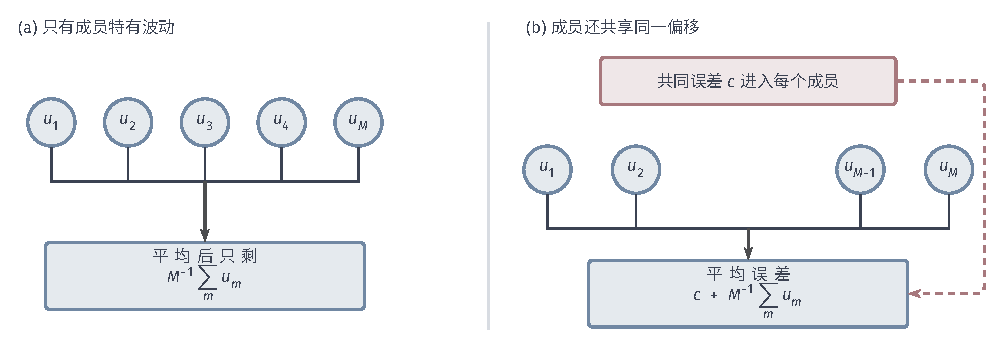
\includegraphics[width=169.000mm]{figures/04-classic-models/00-shared/tikz/ensemble-error-dependence/figure.pdf}
  \caption{成员误差依赖与平均的作用。左图表示只有成员特有波动时，平均可以随成员数增加而削弱这些波动；右图表示所有成员还共享误差$c$时，共同项仍保留在平均预测中。图中成员数量与符号只用于说明机制，不表示实测误差。}
  \label{fig:ensemble-error-dependence}
\end{figure*}

\subsubsection{参数学习}

对第$m$个成员，从$\{1,\ldots,n\}$中独立、等概率、有放回地抽取$n$次索引，所得多重集合记为$I^{(m)}$。有放回抽样使部分记录重复进入成员训练，也使部分记录留在该成员之外。学习算法$\mathcal{A}$在相应自助样本上训练出
\[
  h_m=\mathcal{A}\!\left(D_n^{(m)}\right),
  \qquad
  D_n^{(m)}=\{(\bm{x}_i,y_i):i\in I^{(m)}\}.
\]
回归通常平均$h_m(\bm{x})$；分类可以投票，也可以在成员输出具有同一语义时平均逐类得分或概率。可以改变自助样本大小或采用其他成员算法。此时仍需检验重采样是否使成员在新样本上产生互补预测。

\paragraph{构造袋外预测}

一份大小为$n$的标准自助样本没有抽中原始样本$i$的概率为
\begin{equation}
  \mathbb{P}\!\left(i\notin I^{(m)}\right)
  =
  \left(1-\frac{1}{n}\right)^n
  \longrightarrow e^{-1}.
  \label{eq:ensemble-oob-probability}
\end{equation}
因此，每个成员平均约有$36.8\%$的原始样本未参与其训练。这个副产品非常有用：评估模型通常要另外留出一份验证集，而Bagging免费送来了一份——对某个成员而言，那些它没见过的样本正好可以用来检验它，既不必额外切分数据，也没有浪费训练记录。这些样本构成该成员的\term{袋外样本}（out-of-bag sample, OOB sample）。反过来，对每个训练样本$i$，可以只收集没有使用它训练的成员预测。令
\[
  \mathcal{M}_{i}^{\mathrm{OOB}}
  =\{m:i\notin I^{(m)}\},
\]
当$\mathcal{M}_{i}^{\mathrm{OOB}}$非空时，回归的袋外预测可写为
\begin{equation}
  \widehat{y}_{i}^{\mathrm{OOB}}
  =
  \frac{1}{|\mathcal{M}_{i}^{\mathrm{OOB}}|}
  \sum_{m\in\mathcal{M}_{i}^{\mathrm{OOB}}}h_m(\bm{x}_i),
  \label{eq:ensemble-oob-prediction}
\end{equation}
分类则对同一成员集合投票或平均类别输出。图\ref{fig:ensemble-bagging-oob}按样本收集符合条件的成员：每个样本的袋外预测由其未参与训练的成员子集给出，子集随样本变化。

\begin{figure*}[htbp]
  \centering
  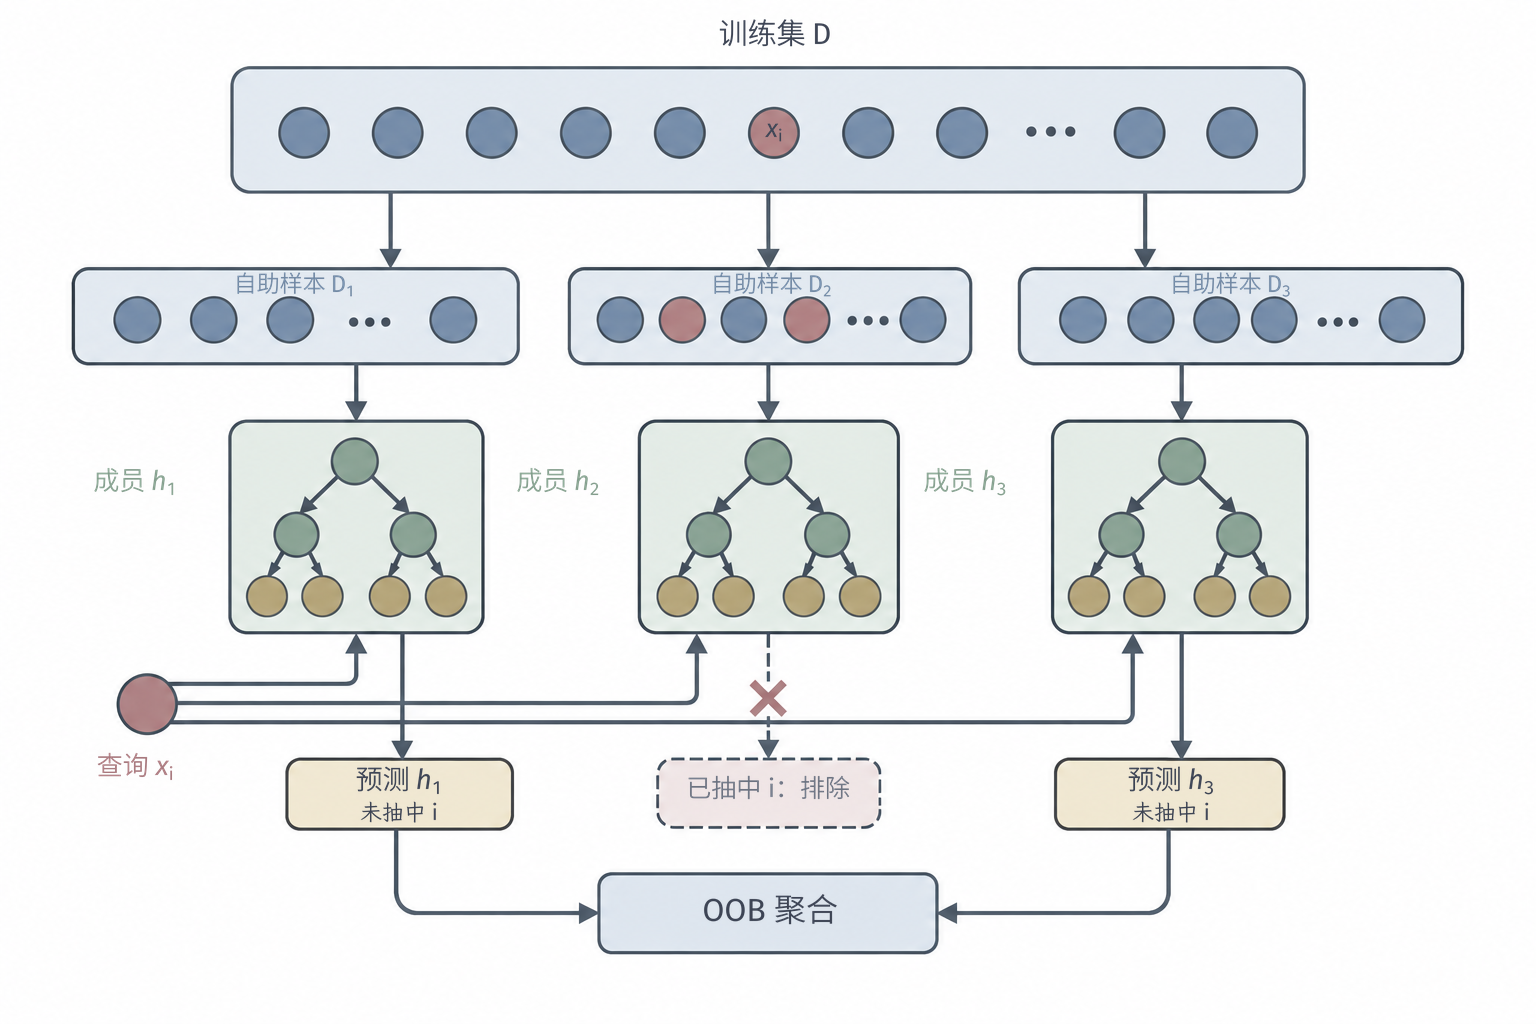
\includegraphics[width=130.048mm]{figures/04-classic-models/00-shared/generated/ensemble-bagging-oob/figure.png}
  \caption{Bagging训练与袋外预测。每个成员只使用其自助样本训练；对训练样本$\bm{x}_i$，袋外预测只聚合未抽中$i$的成员。索引与集合展示样本和成员的对应关系；成员数有限时，各样本得到的袋外预测数量不同。}
  \label{fig:ensemble-bagging-oob}
\end{figure*}

袋外预测使当前标签与产生该预测的成员训练分离，可用于绘制树数—损失曲线、内部误差估计和置换重要性。可用成员数随机变化，自助训练集又相互重叠，这一数据结构与固定折的交叉验证不同。成员数很小时，某些样本可能没有足够的袋外预测。

反复用袋外结果选择结构、树数或特征处理，会使袋外误差成为开发证据；最终冻结流程需要另用测试数据评价。时间序列、分组样本或空间相关数据还要求自助抽样尊重依赖单位；逐行重采样会破坏原有数据结构。袋外结果的解释还依赖抽样单位与未来使用的数据制度。

\paragraph{选择成员规模与训练预算}

给定原数据后，独立的重采样及训练可分配给不同计算单元。评价并行收益时，需要同时计入总工作量与实际经过时间：若单个成员的训练和预测成本分别为$C_{\mathrm{train}}$与$C_{\mathrm{pred}}$，朴素实现的总工作量仍约随$M C_{\mathrm{train}}$和$M C_{\mathrm{pred}}$增长。模型存储也通常随成员数量增加。

在固定训练集上增加独立随机成员，主要减少有限次抽样的Monte Carlo误差；等权平均逐渐逼近该随机训练机制的期望预测。原数据的抽样误差和模型失配仍影响这一期望，共同误差也会留在组合中。实践中可以观察袋外损失随成员数的变化，在曲线趋于稳定后停止增加成员，但这个停止规则也属于模型选择过程。

可以用一个固定输入处的简化误差模型看清这一区别。设第$m$个成员相对真实回归均值的误差为$b+C+U_m$，其中$b$为固定偏差，$C$为所有成员共享的零均值训练数据误差，$U_m$为各自的零均值随机训练误差。假设$C$与各$U_m$不相关，各$U_m$彼此不相关，方差分别为$\tau^2$与$\sigma^2$，则平均预测的均方误差为
\[
 \mathbb E\left(b+C+\frac1M\sum_{m=1}^M U_m\right)^2
 =b^2+\tau^2+\frac{\sigma^2}{M}.
\]
给定训练数据后，各成员的随机数可以独立；重新抽取训练数据时，它们仍会共享$C$，因而预测误差相关。例如$b=0$、$\tau^2=1$、$\sigma^2=3$时，单成员均方误差为4，10个成员平均后为1.3；共同方差1不会随树数消失。这个分解说明平均能消除哪部分波动，不保证任意学习器经Bagging后都降低误差。

单树复杂度控制每份样本上的拟合，树数控制随机预测的平均程度。较深树可以表达更细的分区，也可能对扰动更敏感；叶规模与深度限制则可减少极小叶和噪声标签的影响。叶最小样本量、最大深度、类别权重和自助样本大小仍须与成员数共同选择，尤其在标签噪声、极小叶或类别极不平衡时。

\subsection{随机森林}
\label{sec:ensemble-random-forest}

\subsubsection{模型结构}

树Bagging改变了训练记录，但未必让树的结构有足够差异。例如，房屋面积若在多数自助样本中都是最强的分裂特征，各树就会几乎都先按面积划分，继而在相似区域作出相似错误。回到章首的投票算例：成员越相关，投票收益越小；这些树虽然看到的样本不同，却因为同一个强特征而“想法雷同”，高度相关。增加树数能稳定平均，却不能自动消除成员共同的错误。

\term{随机森林}（random forest）的对策是故意“限制每棵树的视野”：在自助采样之外加入节点级特征随机化，每个节点先随机抽取一组候选特征，只在这组中搜索分裂。面积不在当前候选组时，树就被迫尝试房龄或其他特征，由此长出不同的划分。乍看这让单棵树变差了（它有时用不上最强的特征），但换来的是树与树之间相关性降低，使平均真正发挥作用；这是一个“牺牲单个成员准确度、换取成员多样性”的典型权衡。树仍按第\ref{sec:regression-trees}节或第\ref{sec:classification-trees}节的任务准则形成叶输出；随机化改变的是本次分裂可使用的信息，用来减弱各树对少数强特征的共同依赖\scite{breiman2001randomforests}。

\subsubsection{参数学习}

训练每棵树时，先抽取自助样本，再递归生长各节点：随机选取候选特征，在这些特征上按任务损失搜索分裂，直到达到停止条件，最后计算各叶的预测值。不同树使用各自的抽样与特征随机数，可以分别训练。

节点候选特征数同时影响单树可用的信息和不同树的分裂差异。候选数接近全部特征时，森林更接近普通的树Bagging；候选数较小时，不同树更可能采用不同分裂，但单棵树也更容易错过当前节点上的有效特征。合适的候选规模取决于特征冗余、样本量和树深，可在固定验证协议下比较。

\subsection{极度随机树（Extra Trees）}
\label{sec:ensemble-extra-trees}

\subsubsection{模型结构}

随机森林虽然随机选择候选特征，阈值仍通过当前节点的数据搜索。如果同一个数值特征有很多候选切分点，每棵树仍要承担相应搜索成本，而且不同树可能继续选中接近的最佳阈值。\term{极度随机树}（extremely randomized trees, Extra Trees）进一步随机生成候选切分点，再从这些随机候选中选取得分较好的分裂。它同时减少阈值搜索并增加树之间的差异，代价是单棵树放弃了在全部阈值中寻找最佳分裂。原始方法通常让各树使用完整训练集，把差异主要交给特征与阈值随机化；具体软件也可能允许额外使用自助采样\scite{geurts2006extra}。

\subsubsection{参数学习}

在每个节点，先抽取候选特征，为这些特征生成随机阈值，再按分类不纯度或回归损失比较候选分裂；选定分裂后继续递归，叶输出仍按所属任务估计。阈值的随机生成替代了遍历全部候选值的步骤，训练其他部分沿用树模型。

随机阈值减少了穷举候选切分的工作，也会让单棵树偏离当前样本上的最佳贪心分裂。组合是否改善，取决于单树预测能力下降与成员依赖减弱之间的平衡。候选特征数、每个特征的随机阈值数、叶最小样本量以及是否采用自助采样共同决定这个平衡；增加随机化能否降低测试损失，需要在同一数据与预算下检验。

\subsection{模型对比与总结}
\label{sec:ensemble-bagging-comparison}

图\ref{fig:ensemble-tree-randomization}沿一棵树的构造路径比较三种随机化位置。树Bagging主要改变成员看到的训练样本；随机森林还在每个节点抽取候选特征；Extra Trees继续把随机性放入候选阈值。三者继续以任务准则比较分裂，差别在于进入贪心搜索的样本、特征和阈值。

\begin{figure*}[htbp]
  \centering
  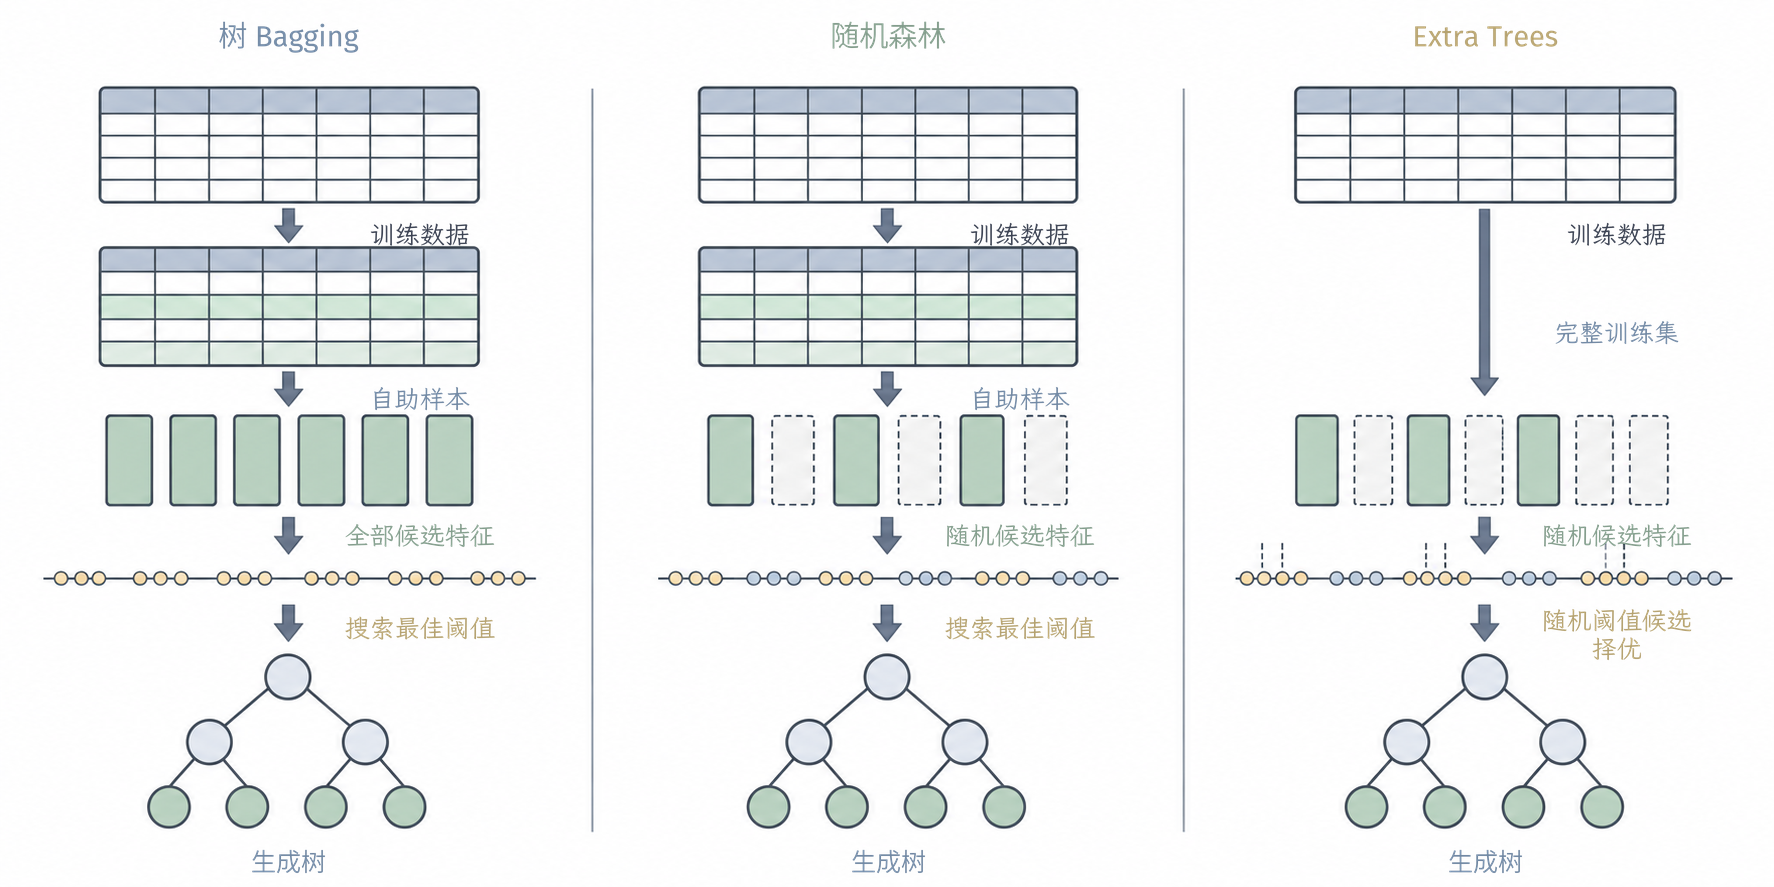
\includegraphics[width=150.199mm]{figures/04-classic-models/00-shared/generated/ensemble-tree-randomization/figure.png}
  \caption{树Bagging、随机森林与Extra Trees的随机化位置。每栏从样本来源出发，依次展示候选特征、候选阈值与成员树；候选选择中的随机性和任务准则约束分别标在相应步骤。每栏首框直接标出训练样本来源：前两栏采用自助采样，Extra Trees栏采用原始方法的完整训练集设定；具体实现也可能额外启用自助采样。}
  \label{fig:ensemble-tree-randomization}
\end{figure*}

三种方法的预测都由树叶输出聚合得到。它们依次改变样本、节点候选特征和候选阈值，训练时仍用任务准则决定分裂与叶值。增加随机化可能减弱共同错误，也可能削弱单树，因此应在相同预算下比较组合预测；表\ref{tab:ensemble-bagging-comparison}列出具体差别。

\begin{table*}[htbp]
  \centering
  \small
  \begin{tabularx}{\linewidth}{@{}>{\raggedright\arraybackslash}p{24mm}*{6}{>{\raggedright\arraybackslash}X}@{}}
    \toprule
    方法 & 样本扰动 & 节点候选特征 & 阈值选择 & 袋外预测 & 成员训练 & 主要边界 \\
    \midrule
    树Bagging & 通常自助采样 & 全部特征 & 在候选中搜索 & 标准自助设定下可用 & 成员间可并行 & 强特征可能使树高度相关 \\
    随机森林 & 通常自助采样 & 随机特征子集 & 在子集内搜索 & 标准自助设定下可用 & 成员间可并行 & 候选数过小会削弱单树 \\
    Extra Trees & 原始方法使用完整训练集；实现可选自助采样 & 随机特征子集 & 生成随机阈值后择优 & 仅在采用自助采样时可用 & 成员间可并行 & 过强随机化会增大单树误差 \\
    \bottomrule
  \end{tabularx}
  \caption{以树为成员时，Bagging、随机森林与Extra Trees的机制比较。表中列出基本构造；比较具体实现时，还需记录抽样设置，并固定树复杂度、成员数和计算预算。}
  \label{tab:ensemble-bagging-comparison}
\end{table*}

原始Extra Trees使用完整训练集，没有标准自助采样形成的袋外预测；若额外启用自助采样，才可按相应未抽中成员构造袋外结果。

Bagging先产生训练差异，再聚合预测以削弱部分波动。固定聚合保留成员共享的遗漏；若希望让新成员针对这些不足训练，就需要根据当前组合产生修正信号。下一节据此转向序贯提升。

\section{基于Boosting的集成}
\label{sec:ensemble-boosting}

Bagging让多个成员分别完成同一个预测任务，再聚合它们的结果。如果这些成员反复在同一批样本上预测偏低，仅增加类似成员并平均，偏低的误差仍会保留。我们可以换一种训练方式：先计算已有组合还错在哪里，再让新成员专门学习一个修正量。

\term{Boosting}（提升）由此构造序贯加法模型：第$t$轮根据已有函数$F_{t-1}$选择新成员及其贡献，以降低指定训练目标。新成员承担的是对已有预测的补充，可以比一个独立完成任务的模型更简单。AdaBoost、梯度提升及现代提升树共享这种逐轮依赖，但它们从错误中提取修正信号的方式不同。

\subsection{前向逐步加法模型}
\label{sec:ensemble-stagewise-additive}

\subsubsection{模型结构}

设$F_0$为初始预测，Boosting经过$T$轮得到
\begin{equation}
  F_T(\bm{x})
  =
  F_0(\bm{x})
  +
  \sum_{t=1}^{T}\alpha_t h_t(\bm{x}),
  \label{eq:ensemble-additive-model}
\end{equation}
其中$h_t$是第$t$个成员，$\alpha_t$控制其贡献。

\subsubsection{参数学习}

为使复杂度惩罚对应真正加入模型的函数，把本轮增量记为$f_t=\alpha_t h_t$。给定损失$\ell$，理想化的第$t$轮直接优化增量：
\begin{equation}
  f_t
  \in
  \argmin_{f\in\mathcal{F}}
  \sum_{i=1}^{n}
  \ell\!\left(
    y_i,
    F_{t-1}(\bm{x}_i)+f(\bm{x}_i)
  \right)
  +\Omega_t(f).
  \label{eq:ensemble-forward-stagewise}
\end{equation}
这里$\mathcal{F}=\{\alpha h:\alpha\in\mathbb{R},h\in\mathcal{H}\}$是由成员函数族$\mathcal{H}$生成的增量函数族，$\Omega_t$是相应复杂度惩罚，也可以取零。

树的叶数惩罚控制分区规模，叶输出范数惩罚控制本轮增量。范数应作用于$f$，使惩罚随实际加入组合的幅度变化；若仅惩罚$h$，它与$\alpha$的相互缩放会改变惩罚却保持预测。

逐步优化固定已有成员，减少了联合搜索变量，但最优范围仅限本轮增量。后文用梯度拟合、二阶目标和收缩构造近似更新。

不同方法将当前预测转换为不同的训练信号。AdaBoost改变训练样本的权重，使当前错分记录在下一轮具有更大影响；梯度提升把损失对当前预测的负梯度作为伪响应；二阶提升树还利用局部曲率近似叶权重和分裂收益。平方损失的负梯度恰为普通响应残差，其他损失则给出不同修正量。损失决定了下一轮成员拟合的对象。

\subsection{AdaBoost}
\label{sec:ensemble-adaboost}

\subsubsection{模型结构}

先考虑二分类。如果每轮都用相同权重训练一个简单分类器，容易分类的多数样本可能反复决定边界，而少量错分样本始终得不到修正。\term{AdaBoost}（adaptive boosting）让错分记录在下一轮占更大权重，使新分类器更多地处理这些记录；同时根据本轮分类器的加权错误率确定它在组合中的贡献。这样，训练下一成员所面对的数据权重会随前面成员的预测改变。

模型以二分类函数作为成员，用加权得分$F_T(\bm{x})=\sum_{t=1}^T\alpha_t h_t(\bm{x})$表示组合，按其正负输出类别。每个成员只给出一个类别判断，投票权重决定该判断在组合中的作用。

\subsubsection{参数学习}

取标签$y_i\in\{-1,1\}$和成员$h_t(\bm{x})\in\{-1,1\}$。初始样本权重为$w_i^{(1)}=1/n$，第$t$轮成员的加权错误率为
\begin{equation}
  \epsilon_t
  =
  \sum_{i=1}^{n}
  w_i^{(t)}
  \mathbb{I}\!\left\{y_i\neq h_t(\bm{x}_i)\right\}.
  \label{eq:ensemble-adaboost-error}
\end{equation}
当$0<\epsilon_t<1/2$时，成员投票权重取
\begin{equation}
  \alpha_t
  =
  \frac{1}{2}
  \log\frac{1-\epsilon_t}{\epsilon_t},
  \qquad
  w_i^{(t+1)}
  =
  \frac{
    w_i^{(t)}
    \exp\!\left[-\alpha_t y_i h_t(\bm{x}_i)\right]
  }{Z_t},
  \label{eq:ensemble-adaboost-update}
\end{equation}
其中$Z_t$使新权重和为1。错分样本满足$y_i h_t(\bm{x}_i)=-1$，权重乘上$e^{\alpha_t}$；正确样本的权重乘上$e^{-\alpha_t}$。

若$\epsilon_t=0$，在这些正权重下当前成员已分对全部训练样本，便直接输出$h_t$并停止，避免将发散系数代入更新（参考\BookSectionRef{sec:boosting}{卷3《基础、理论与可信性》第5章“二分类学习的可学习性”第5.6节“集成学习”}）。其余情况下，最终分类器在预先固定平局规则后按$\operatorname{sign}(\sum_t\alpha_t h_t(\bm{x}))$决策。正的成员贡献要求当前加权错误率小于$1/2$；条件未满足时，可停止本轮、调整训练或采用相应变体。

图\ref{fig:ensemble-adaboost-weight-update}将分类错误与下一轮权重连接起来。当前分类结果先改变样本权重，再由归一化后的权重决定下一轮成员看到的训练分布；错分记录因而获得更大的后续影响。

\begin{figure*}[htbp]
  \centering
  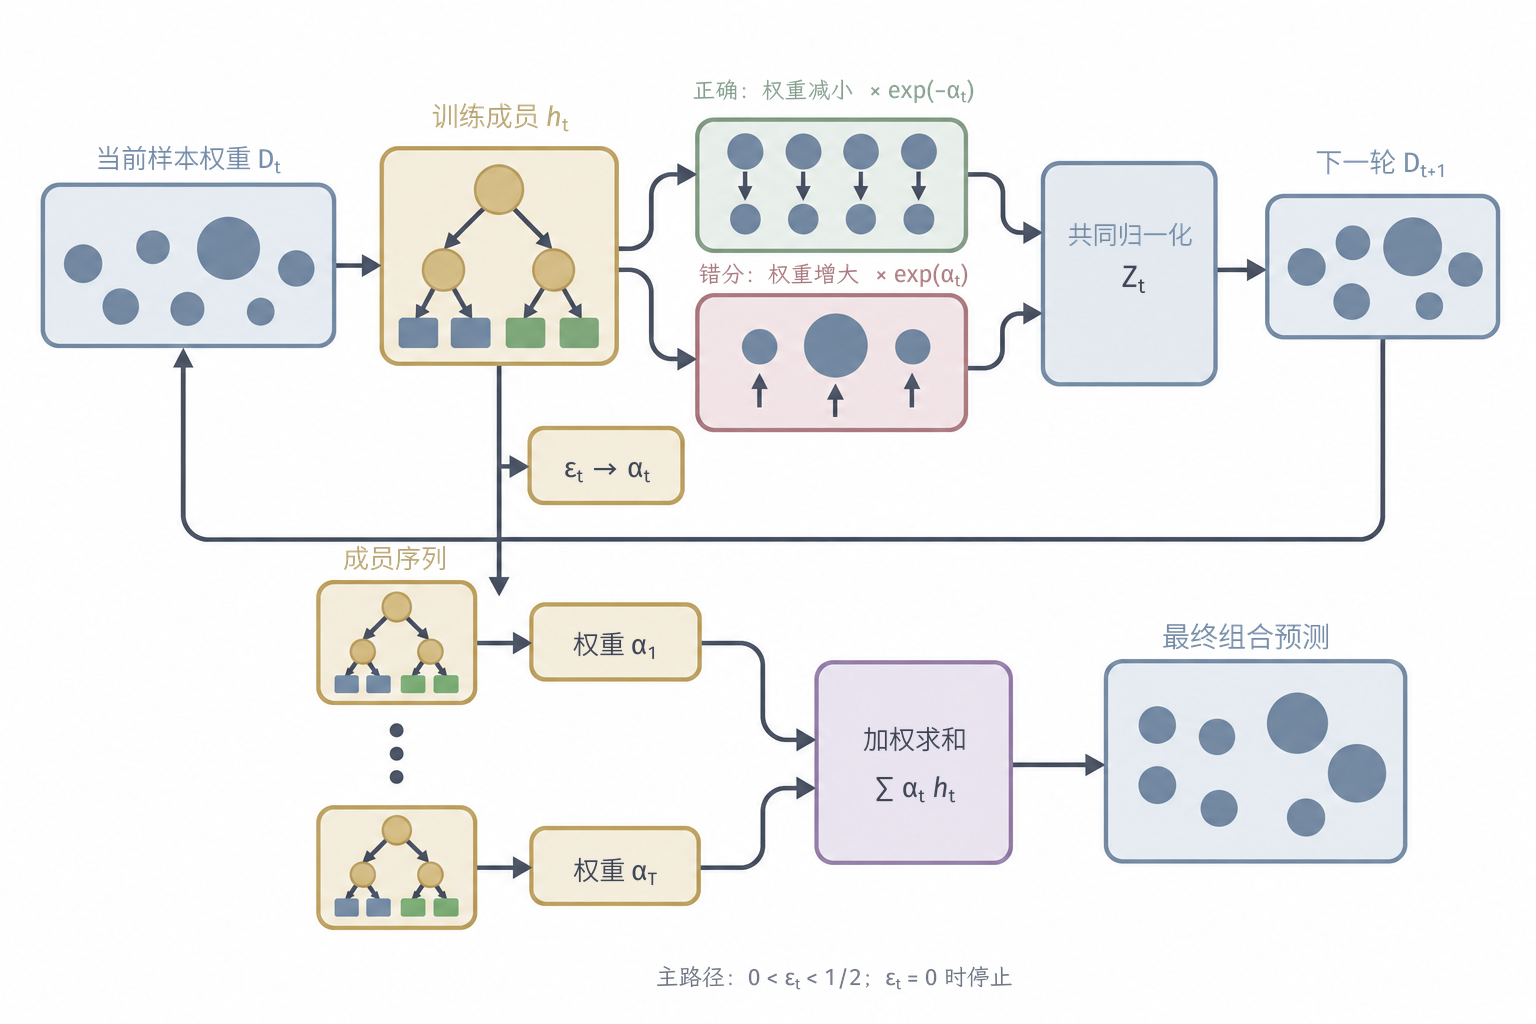
\includegraphics[width=130.048mm]{figures/04-classic-models/00-shared/generated/ensemble-adaboost-weight-update/figure.png}
  \caption{AdaBoost的样本权重更新。分类结果把样本分成正确与错分两路，两路缩放后的权重汇合并归一化，形成下一轮训练分布。实线连接各更新步骤；绿色框标示正确分类样本的减权，红色框标示错分样本的增权。}
  \label{fig:ensemble-adaboost-weight-update}
\end{figure*}

这一更新也可以从指数损失解释。令$F(\bm{x})=\sum_t\alpha_t h_t(\bm{x})$，经验目标为
\[
  \sum_{i=1}^{n}\exp\!\left[-y_iF(\bm{x}_i)\right].
\]
固定$F_{t-1}$后选择$h_t$与$\alpha_t$，在$0<\epsilon_t<1/2$时可以导出式\eqref{eq:ensemble-adaboost-update}。样本重加权由指数损失的逐步优化导出，因此其作用可以通过该目标分析\scite{freund1997boosting,friedman2000adaboost}。

\subsubsection{支持多分类预测场景}

二分类AdaBoost把每个成员的输出编码为$-1$或$+1$，最后用加权得分的正负判类。类别超过两个时，这个标量符号已经不能表示类别竞争。多分类变体需要让成员输出类别或逐类得分，再通过相应的加权投票或得分组合决定类别；样本重加权也要与所选多类损失一致。二分类中要求成员错误率低于$1/2$的条件及其系数公式不能直接沿用，必须按新的类别竞争方式重新推导。

\subsubsection{支持类别概率预测场景}

投票符号只回答类别，许多任务还需要输出事件发生的概率。LogitBoost从加法Logistic回归出发，用二项对数损失确定逐轮更新，再将累积得分转换为概率。它与AdaBoost都逐步加入成员，但修正量来自不同损失；转换后的概率是否准确，仍需根据样本外概率损失和校准情况判断\scite{friedman2000adaboost}。下一节给出一般损失如何导出修正信号的统一构造。

\subsection{梯度提升机与GBDT}
\label{sec:ensemble-gradient-boosting}

\subsubsection{模型结构}

AdaBoost用分类错误调整样本权重，但回归还需要描述“错了多少、向哪边修正”。例如，一个响应为100的样本当前预测为80，平方损失下需要向上修正；另一个响应同为100、当前预测为120的样本则需要向下修正。仅给两条记录增加相同权重，没有直接告诉新成员这两个相反方向。

对于关于预测可微的损失，负梯度给出了每个训练预测降低损失的方向。\term{梯度提升机}（gradient boosting machine, GBM）用基学习器拟合这些负梯度，再把学得的修正加入已有预测。取平方损失$\ell(y,F)=(y-F)^2/2$时，负梯度就是残差$y-F$，其他损失则产生各自的修正信号；序贯加法因而可以用于更一般的任务\scite{friedman2001gradientboost}。

GBM沿用式\eqref{eq:ensemble-additive-model}的加法结构，成员输出连续修正量。成员取回归树时，就是\term{梯度提升决策树}（gradient boosting decision tree, GBDT）；每片叶输出一个常数修正，全部树的修正叠加形成最终得分或数值预测。

\subsubsection{参数学习}

通常从使训练损失最小的常数预测开始：
\begin{equation}
  F_0(\bm{x})=c_0,
  \qquad
  c_0\in\argmin_c\sum_{i=1}^{n}\ell(y_i,c).
  \label{eq:ensemble-gbm-initialization}
\end{equation}
平方损失下$c_0$是响应均值。这里要求存在有限的最小化点；若某种损失与数据组合使最优常数趋于无穷，就需约束预测范围或另定有限初始化。

在第$t$轮，对每个训练样本计算\term{伪残差}（pseudo-residual），即损失在当前预测处的负导数：
\begin{equation}
  r_i^{(t)}
  =
  -
  \left.
  \frac{\partial \ell(y_i,z)}{\partial z}
  \right|_{z=F_{t-1}(\bm{x}_i)}.
  \label{eq:ensemble-pseudo-residual}
\end{equation}
随后用平方误差把这些修正量拟合到成员函数族：
\begin{equation}
  h_t\in\argmin_{h\in\mathcal{H}}
  \sum_{i=1}^{n}\bigl(r_i^{(t)}-h(\bm{x}_i)\bigr)^2.
  \label{eq:ensemble-gbm-gradient-fit}
\end{equation}
此处平方误差衡量成员对负梯度的逼近，即使原任务采用其他损失也使用这一拟合对象。贪心树生长通常给出子问题的近似解。

固定$h_t$后，可以按原损失做整体线搜索，在最小值存在时取
\begin{equation}
  \alpha_t\in\argmin_\alpha
  \sum_{i=1}^{n}
  \ell\!\left(y_i,F_{t-1}(\bm{x}_i)+\alpha h_t(\bm{x}_i)\right).
  \label{eq:ensemble-gbm-line-search}
\end{equation}
此处$\alpha_t$是整棵树或整个成员共享的一个标量。加入预先选择的收缩系数$\eta\in(0,1]$后，
\begin{equation}
  F_t(\bm{x})
  =
  F_{t-1}(\bm{x})
  +
  \eta\alpha_t h_t(\bm{x}).
  \label{eq:ensemble-gradient-boosting-update}
\end{equation}


当$\ell(y,z)=\tfrac12(y-z)^2$时，式\eqref{eq:ensemble-pseudo-residual}给出$y_i-F_{t-1}(\bm{x}_i)$，恰好是普通残差。图\ref{fig:ensemble-boosting-residuals}展示一次这样的更新：新成员拟合的是第二幅图中的残差，再把它的输出加回已有预测。左侧原本偏高的预测随负残差降低，右侧原本偏低的预测随正残差升高；这组数据的平均平方损失也随之下降。

\begin{figure*}[tbp]
  \centering
  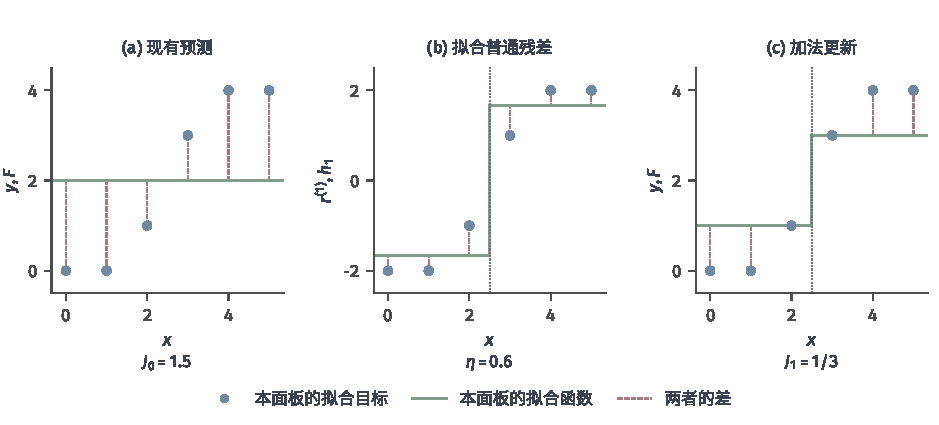
\includegraphics[width=159.000mm]{figures/04-classic-models/00-shared/matplotlib/ensemble-boosting-residuals/figure.pdf}
  \caption{平方损失下的一次梯度提升更新。六个输入为$x=0,\ldots,5$，响应依次为$0,0,1,3,4,4$，常数初始化$F_0=2$。在相邻输入中点中搜索，最小二乘残差树选取阈值$2.5$，两叶输出分别为$-5/3$与$5/3$。取$\eta=0.6$，$F_1=F_0+\eta h_1$在两侧分别为$1$与$3$；平均损失$J_t=(2n)^{-1}\sum_i[y_i-F_t(x_i)]^2$由$1.5$降至$1/3$。蓝点依次表示观测、残差、观测，绿线为各面板的拟合函数，红色虚线为两者之差。数据与更新均为可复核的教学构造，这个普通残差计算依赖平方损失。}
  \label{fig:ensemble-boosting-residuals}
\end{figure*}

分类时则要先明确得分与概率的关系。例如二分类采用$y_i\in\{0,1\}$，令$F$表示对数几率（logit），相应概率与二项对数损失为
\[
  p=\sigma(F)=\frac{1}{1+e^{-F}},\qquad
  \ell(y,F)=\log(1+e^F)-yF.
\]
由于$\partial\ell/\partial F=\sigma(F)-y$，第$t$轮的伪残差为
\[
  r_i^{(t)}=y_i-p_i^{(t-1)},\qquad
  p_i^{(t-1)}=\sigma\!\left(F_{t-1}(\bm{x}_i)\right).
\]


例如$y_i=1$而当前概率为$0.3$时，伪残差为$0.7$，表示损失对得分的修正信号。成员拟合后将增量加到$F$，再经Sigmoid换算概率；修正量与概率因此处于不同数值空间。

对于GBDT，除了整体线搜索，还可以保留平方拟合得到的叶区域$\bm{R}_1^{(t)},\ldots,\bm{R}_{L_t}^{(t)}$，再按原损失分别求每片叶的增量。当各叶内存在有限最小化点时，
\begin{equation}
  \begin{aligned}
    v_j^{(t)}
      &\in\argmin_v
        \sum_{i:\,\bm{x}_i\in\bm{R}_j^{(t)}}
        \ell\!\left(y_i,F_{t-1}(\bm{x}_i)+v\right),\\
    F_t(\bm{x})
      &=F_{t-1}(\bm{x})
        +\eta\sum_{j=1}^{L_t}
        v_j^{(t)}\mathbb{I}\{\bm{x}\in\bm{R}_j^{(t)}\}.
  \end{aligned}
  \label{eq:ensemble-gbm-leaf-update}
\end{equation}
$L_t$表示叶数，各叶分别选择$v_j^{(t)}$并替换原树输出；这与整棵树共用一个$\alpha_t$是两种更新方案。有限叶内最小值不存在时，需要限制输出或增加正则后再更新。回归树在这里承担连续修正量的拟合，最终任务也可以是分类。

\subsubsection{优化泛化能力}

\paragraph{控制逐轮更新幅度与模型复杂度}
学习率、轮数与单树复杂度共同决定加法函数。较小学习率缩小每轮变化，通常需要更多轮才能达到相近训练目标；较深的树可以在单轮表达更高阶交互，也会扩大每轮容量。行采样和列采样进一步引入随机性，早停则依据独立验证轨迹选择轮数。选择学习率时需同时调整轮数，并在给定树复杂度、采样和早停协议下比较。

\paragraph{减弱逐轮拟合对训练样本的依赖}
每轮都使用全部训练样本时，提升树可能反复追踪其中的偶然起伏。随机梯度提升在每轮只用一个随机子样本拟合新成员，使不同轮次面对的记录有所变化。它保留负梯度修正的目标，同时减少本轮参与拟合的样本数。子样本比例过低也可能使修正方向更不稳定，因此采样比例需要与学习率、轮数及树复杂度共同选择\scite{friedman2002stochastic}。

\paragraph{减弱新增成员对既有树的依赖}
提升的后期成员面对的是已有组合留下的残差，可能只修正少量记录，越来越依赖前面树的具体输出。DART在本轮计算修正信号时暂时移除一部分已有树，让新树补充这个不完整组合的预测。加入新树后，算法还会调整新树和被移除树的贡献，再将它们放回组合，避免补回同一缺口时使更新幅度过大。这里扰动的是已有预测，随机梯度提升扰动的则是本轮样本；两者可分别改变新成员依赖的信息，收益仍取决于扰动强度和任务\scite{rashmi2015dart}。

\subsubsection{支持分位数预测场景}

平方损失关注条件均值；若希望按允许的缺货概率确定库存阈值，或预测收入分布中的较低分位点，就需要条件分位数。把第\ref{sec:regression-quantiles}节的分位数损失$\ell(y,z)=\rho_\tau(y-z)$用于提升，成员便学习怎样减少这个分位数目标的偏差。由于损失在$z=y$处不可微，修正信号改用负次梯度，例如约定
\begin{equation}
  r_i^{(t)}
  =\tau-\mathbb{I}\{y_i<F_{t-1}(\bm{x}_i)\},
  \qquad 0<\tau<1.
  \label{eq:ensemble-quantile-pseudo-residual}
\end{equation}
等号处的负次梯度可取$[\tau-1,\tau]$内任意值，这里选端点$\tau$。常数初始化取样本$\tau$分位数，仍用平方误差拟合上述修正量；逐叶更新则最小化原分位数损失，故$v_j^{(t)}$取该叶内普通残差$y_i-F_{t-1}(\bm{x}_i)$的$\tau$分位数，而不是伪残差的均值。

\subsection{XGBoost}
\label{sec:ensemble-xgboost}

\subsubsection{模型结构}

前面介绍的梯度提升用负梯度决定修正方向。用树拟合时，还要选择怎样划分叶区域，以及每个叶应当输出多大的修正。只看当前梯度，没有直接利用损失随修正幅度弯曲的程度；若不断增加叶节点来追逐小幅训练收益，树也可能把样本噪声保留下来。

\term{XGBoost}把叶数和叶权重惩罚写入加法树目标，再用损失的二阶局部近似为叶输出和候选分裂评分。梯度描述向哪边修正，曲率参与决定修正幅度，正则项则限制这次修正使用多复杂的树。大规模训练还要处理稀疏特征、候选阈值与内存访问，原论文围绕这些计算设计了相应系统\scite{chen2016xgboost}。

\subsubsection{参数学习}

设第$t$棵树为$f_t$，损失在当前预测$F_{t-1}(\bm{x}_i)$处的一阶导与二阶导分别为$g_i^{(t)}$和$s_i^{(t)}$。去掉与$f_t$无关的常数后，本轮目标近似为
\begin{equation}
  \widetilde{\mathcal{L}}^{(t)}
  =
  \sum_{i=1}^{n}
  \left[
    g_i^{(t)}f_t(\bm{x}_i)
    +\frac{1}{2}s_i^{(t)}f_t^2(\bm{x}_i)
  \right]
  +\gamma L
  +\frac{\lambda}{2}\sum_{j=1}^{L}v_j^2,
  \label{eq:ensemble-xgboost-objective}
\end{equation}
其中$L$是叶数，$v_j$是第$j$片叶的输出，$\gamma$惩罚新增叶，$\lambda$约束叶权重。若$I_j$表示落入第$j$片叶的样本索引，记
\[
  G_j=\sum_{i\in I_j}g_i^{(t)},
  \qquad
  S_j=\sum_{i\in I_j}s_i^{(t)}.
\]
在$S_j+\lambda>0$时，固定树结构的最优叶权重为
\begin{equation}
  v_j^\star=-\frac{G_j}{S_j+\lambda}.
  \label{eq:ensemble-xgboost-leaf-weight}
\end{equation}
把一个父叶分成左右子叶时，相应近似目标下降量为
\begin{equation}
  \operatorname{Gain}
  =
  \frac{1}{2}
  \left[
    \frac{G_{\mathrm{L}}^2}{S_{\mathrm{L}}+\lambda}
    +
    \frac{G_{\mathrm{R}}^2}{S_{\mathrm{R}}+\lambda}
    -
    \frac{(G_{\mathrm{L}}+G_{\mathrm{R}})^2}
         {S_{\mathrm{L}}+S_{\mathrm{R}}+\lambda}
  \right]
  -\gamma.
  \label{eq:ensemble-xgboost-split-gain}
\end{equation}
式\eqref{eq:ensemble-xgboost-split-gain}把当前损失的梯度、曲率与树复杂度放在同一个分裂准则中。增益评价局部二阶目标在当前分裂下的变化；贪心生长只搜索逐步形成的结构。

图\ref{fig:ensemble-gradient-xgboost}把一阶梯度提升与XGBoost的二阶树评分放在同一计算链中。左图用负梯度定义拟合对象，右图从候选区域的梯度统计计算叶权重和分裂增益；二阶统计扩展了本轮目标的近似信息，但没有改变逐轮加法更新的外层结构。

\begin{figure*}[htbp]
  \centering
  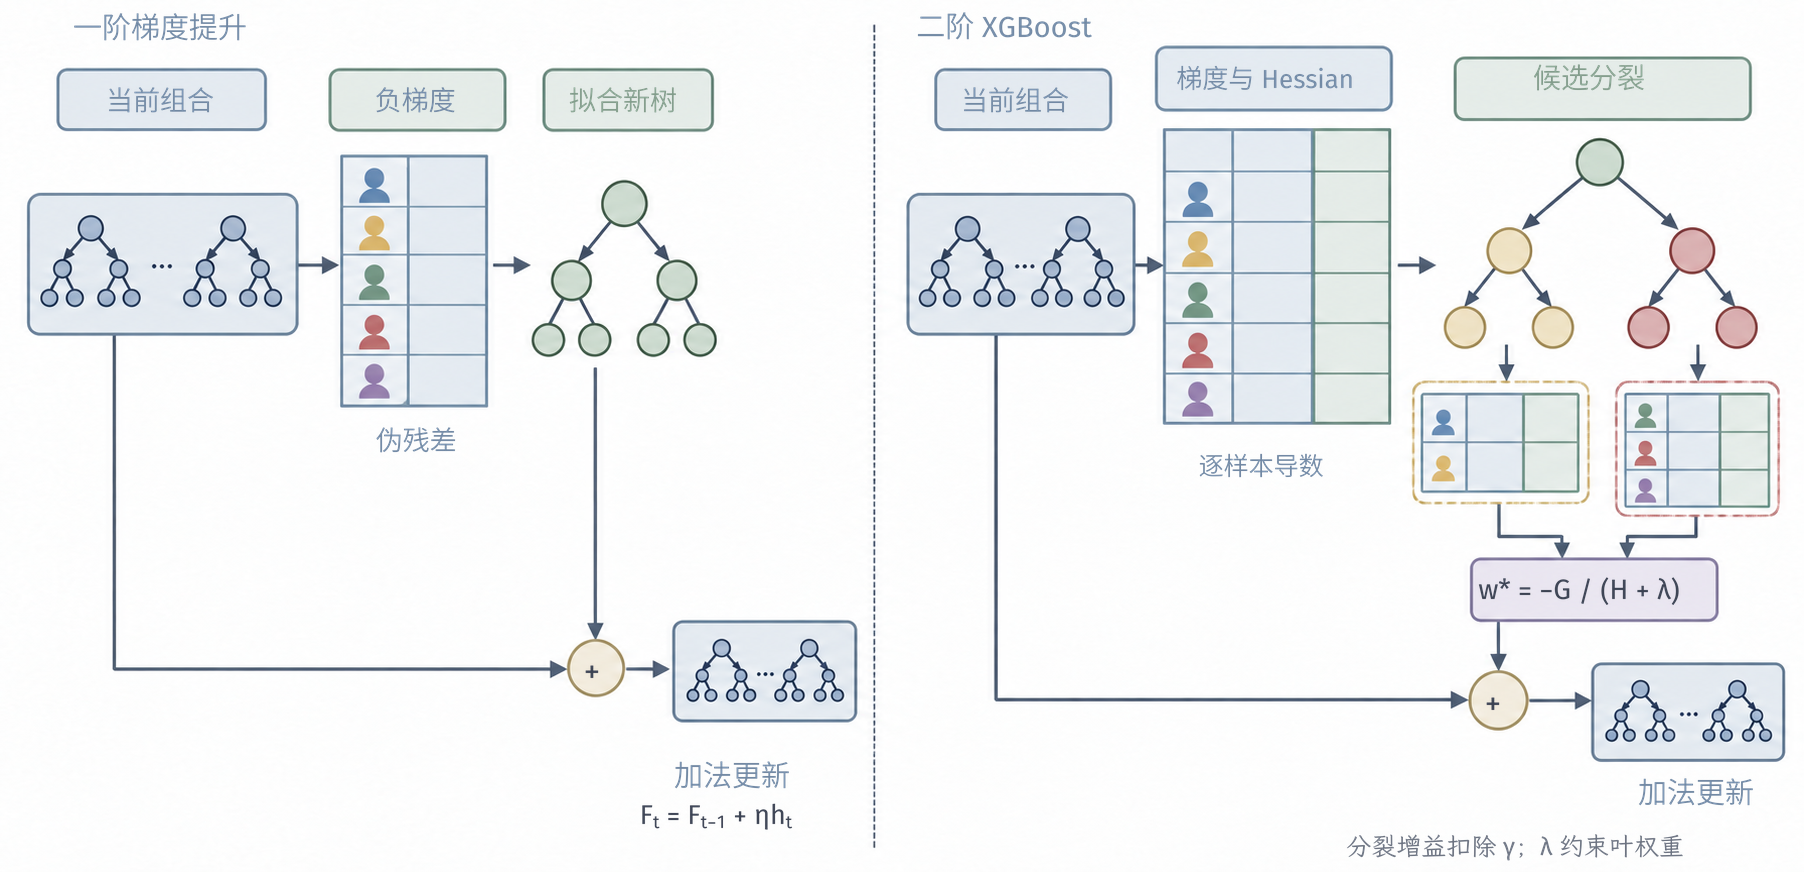
\includegraphics[width=152.739mm]{figures/04-classic-models/00-shared/generated/ensemble-gradient-xgboost/figure.png}
  \caption{梯度提升与XGBoost中的本轮修正。左图中，损失对当前预测的负梯度形成伪残差，新成员拟合该信号后更新组合；右图中，XGBoost按候选分裂聚合一阶导与二阶导，再由同一组叶统计计算叶权重和分裂增益。图中单叶权重$w^\ast$对应正文的$v_j^\star$，$G$与$H$分别表示叶内一阶导和二阶导之和。复杂度项$\gamma T+\lambda\lVert\bm{w}\rVert_2^2/2$中的$T$为叶数，$\bm{w}$汇集各叶输出；$\lambda$限制叶权重，$\gamma$惩罚新增叶。该图展示当前候选树的局部评分。}
  \label{fig:ensemble-gradient-xgboost}
\end{figure*}

\subsubsection{优化计算能力}

\paragraph{减少分裂搜索与数据访问}

精确分裂搜索遍历排序后的候选特征值；近似搜索则先用带权分位数草图构造候选切分，再汇总梯度统计。稀疏感知搜索为缺失值学习默认方向，列采样减少每轮需要检查的特征。块式存储、缓存感知访问、并行统计和外存计算改变的是实现代价，不改变式\eqref{eq:ensemble-xgboost-objective}所定义的学习对象。这些设计在特定硬件和数据规模上的时间收益可通过完整训练测量确认。

\Needspace{10\baselineskip}
\subsection{LightGBM}
\label{sec:ensemble-lightgbm}

\subsubsection{模型结构}

LightGBM仍以回归树的加法组合作为预测函数，树叶输出修正量，最终按任务所需把累计得分转换为预测。它主要改变如何在大规模数据上训练这些树。候选分裂的搜索可能成为提升树训练的主要成本。假设当前节点的一个连续特征有十万个不同取值，精确搜索就可能需要比较近十万个切分位置；每棵新树都会再次进行类似计算。\term{LightGBM}以直方图训练为基础，先把连续特征映射到有限个桶，再按桶累计梯度和曲率。如果使用256个桶，分裂评分就只在相邻桶之间比较，原来同桶内的差别被暂时忽略。

\subsubsection{参数学习}

构造直方图仍要访问节点样本，但候选搜索只需扫描桶。已知父节点和一个子节点的直方图时，还可以用差分得到另一个子节点的统计量。分桶减少存储和候选数，也引入离散化误差；桶数决定这种取舍。

树的生长顺序进一步改变计算分配。按层生长同时扩展某一深度上的叶，按叶生长则每次选择当前增益最大的叶继续分裂。在相同叶数下，后者把容量集中到训练目标下降较大的局部区域，可能形成深度不均衡的树。叶数、最小叶样本量和深度共同限制这种局部扩展，训练收益再由验证或测试检查其样本外效果。

\subsubsection{优化计算能力}

\paragraph{减少样本统计量}

基本直方图训练仍需统计大量样本和特征。LightGBM论文进一步提出两种针对这些成本的近似。\term{单边梯度采样}（gradient-based one-side sampling, GOSS）保留绝对梯度较大的样本，从绝对梯度较小的样本中随机抽取一部分，并在分裂统计中重新加权后者。例如，在小梯度组内等概率抽取一半样本，就把被抽中者对梯度和的贡献乘二，以补偿未采样部分。一般地，样本以概率$p>0$被保留时，其贡献乘以$1/p$；给定本轮梯度和候选分区，这种逆包含概率加权可无偏估计相应的梯度和，平方、比值及择优得到的增益则是非线性量，其偏差需另行分析。

\paragraph{减少有效特征数}

\term{互斥特征捆绑}（exclusive feature bundling, EFB）把很少同时非零的稀疏特征编码到较少的组合特征中，近似减少有效特征数。GOSS、EFB和直方图分别减少样本统计、特征表示和阈值候选，可按各自近似对象评价误差与计算节省\scite{ke2017lightgbm}。

图\ref{fig:ensemble-lightgbm-approximations}按近似对象并列这三种机制。直方图压缩候选阈值，GOSS压缩参与分裂统计的样本，EFB压缩稀疏特征表示；这三个对象分别对应数据访问、有效特征数与候选扫描的成本。

\begin{figure*}[t]
  \centering
  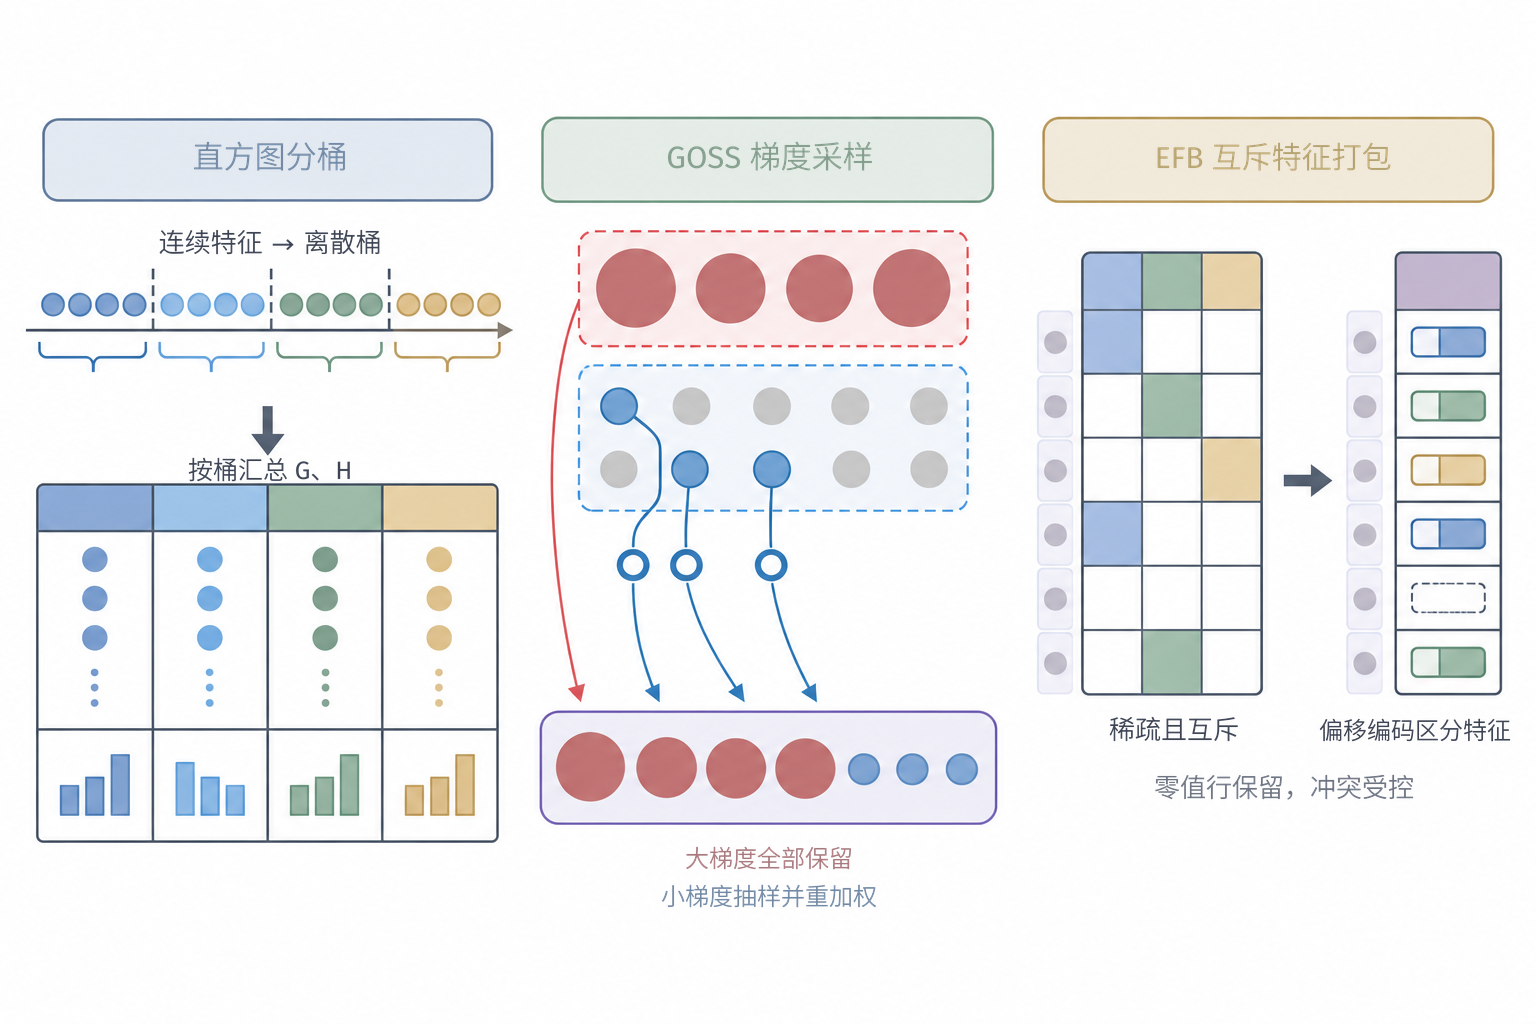
\includegraphics[width=130.048mm]{figures/04-classic-models/00-shared/generated/ensemble-lightgbm-approximations/figure.png}
  \caption{LightGBM中三种作用位置不同的计算近似。直方图把连续取值映射到有限桶，GOSS保留$|g_i|$较大的样本，并抽取、重加权部分$|g_i|$较小的样本，EFB把很少同时非零的特征编码为较少的捆绑特征。图中点数、桶数与非零位置均为机制示意。}
  \label{fig:ensemble-lightgbm-approximations}
\end{figure*}

这些机制的效果依赖梯度分布、特征稀疏性、桶数、冲突处理和硬件实现。比较速度和任务损失时，需要记录数据规模、硬件、桶数与采样设置，并固定搜索预算及早停规则。论文实验的结论据此限定于相应条件。GOSS对固定候选分区的梯度统计可以无偏，并不意味着据此选出的模型已经获得较低的期望风险。

\subsection{CatBoost}
\label{sec:ensemble-catboost}

\subsubsection{模型结构}

类别特征又带来不同的困难。例如商户标识可能有很多取值，全部展开为独热变量会增加特征规模，直接编成整数又会引入原本不存在的次序。用同类别记录的响应均值编码，可以把类别转成一个数，却容易把标签带回输入：某个商户若只有一条记录，包含该记录自身的响应均值恰好就是$y_i$，训练模型于是能直接读到待预测值。新记录的标签还未知，部署时无法提供同样信息。这种把待预测响应用于训练输入的构造称为\term{目标泄漏}（target leakage）。

\term{CatBoost}仍通过逐轮相加的树模型形成预测，并为类别特征安排避免当前标签泄漏的编码过程。它常使用\term{对称树}（symmetric tree），即同一深度的所有节点采用相同分裂条件。深度为$d_{\mathrm{tree}}$的完整对称树至多有$2^{d_{\mathrm{tree}}}$片叶，路径可以编码为固定长度的二进制选择。这种结构便于批量预测，也限制了单棵树可表达的分区形状。

\subsubsection{参数学习}

CatBoost用随机排列建立\term{有序目标统计}（ordered target statistic）。设$c_i$为样本$i$的某个类别值，用$\pi(j)$表示样本$j$在随机排列中的位置；对当前样本只使用排列中位于它之前且类别相同的记录：
\begin{equation}
  z_i
  =
  \frac{
    \sum_{j:\,\pi(j)<\pi(i)}
    \mathbb{I}\{c_j=c_i\}y_j
    +ap
  }{
    \sum_{j:\,\pi(j)<\pi(i)}
    \mathbb{I}\{c_j=c_i\}
    +a
  }.
  \label{eq:ensemble-catboost-ordered-statistic}
\end{equation}
其中$p$是先验统计量，$a>0$控制平滑。前缀统计排除了样本自身的标签，部署时可从已观测的训练记录形成同类别统计。低频类别仍会产生较大估计波动，平滑、多个排列和类别组合需要共同考虑。

图\ref{fig:ensemble-catboost-ordered-statistics}固定当前样本的排列位置，检查哪些标签进入编码。计算当前类别$A$样本的编码时，只允许排列前缀中同为类别$A$的标签进入统计量；其他类别、当前标签和排列后缀都不参与这次编码。

\begin{figure*}[htbp]
  \centering
  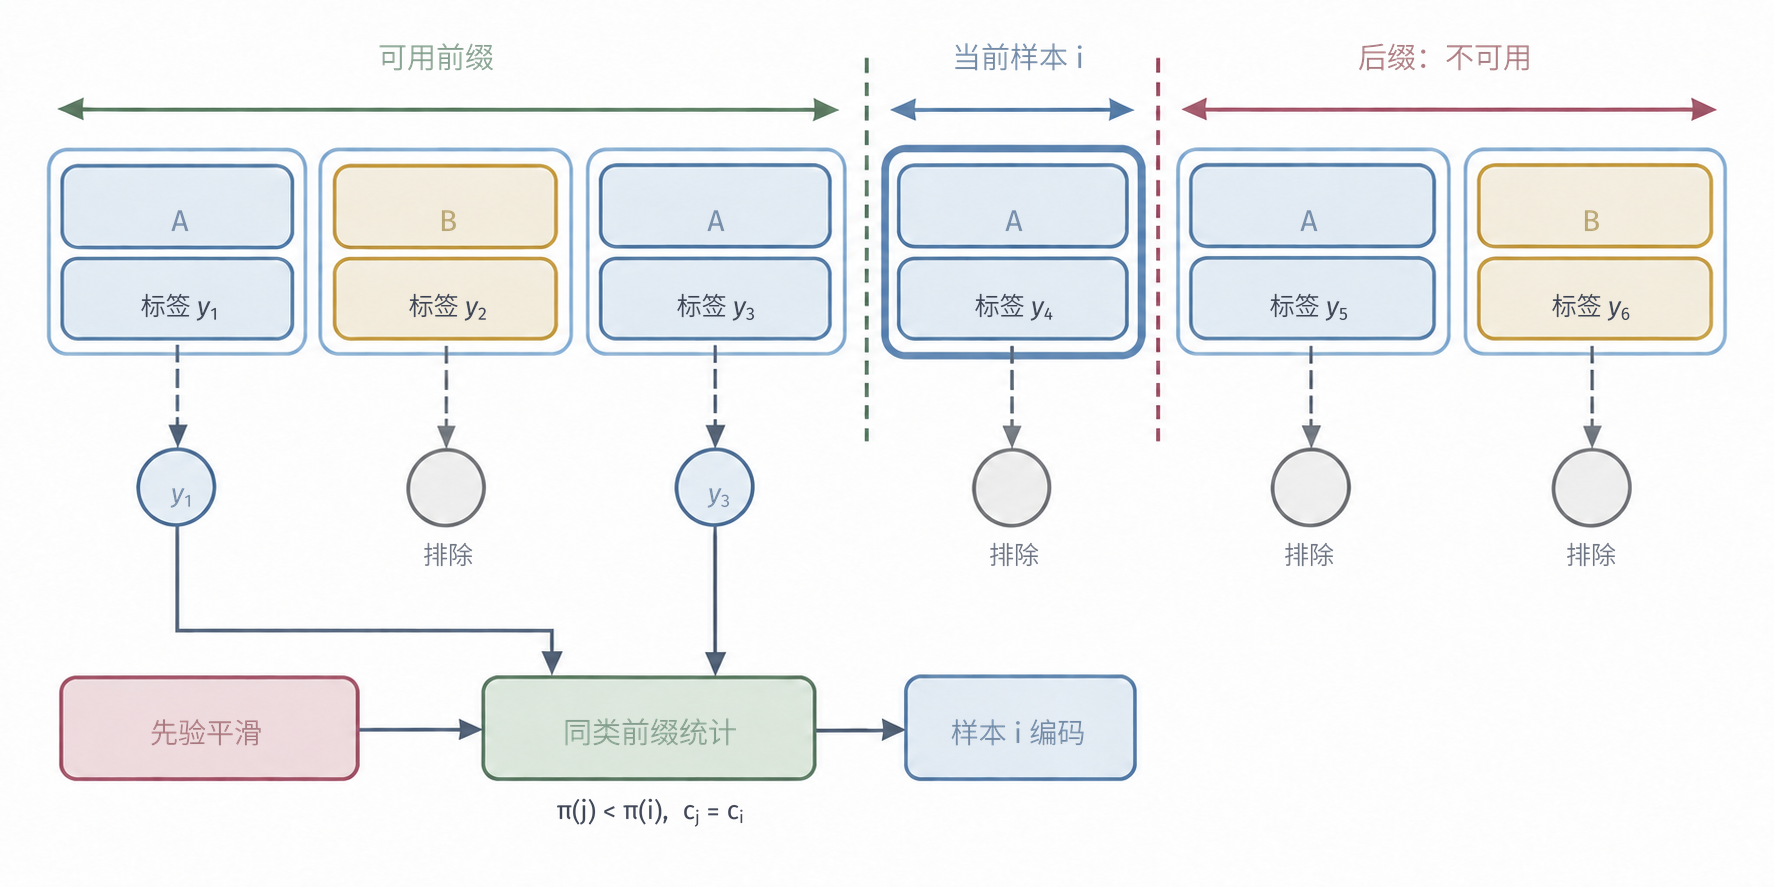
\includegraphics[width=150.199mm]{figures/04-classic-models/00-shared/generated/ensemble-catboost-ordered-statistics/figure.png}
  \caption{CatBoost有序目标统计的前缀约束。这里$\pi(j)$表示样本$j$在随机排列中的位置；计算当前样本$i$的编码时，只有满足$\pi(j)<\pi(i)$且$c_j=c_i$的标签通过实线汇入统计量。其他类别、当前标签和后续记录均不连接到统计量，表示它们在本次编码中被隔离。样本索引与类别符号仅用于说明机制。}
  \label{fig:ensemble-catboost-ordered-statistics}
\end{figure*}

有序提升把相同的前缀思想用于梯度估计。计算当前样本的预测与梯度时，采用由其前缀记录拟合的相应模型，使该样本的标签与当前预测拟合分离，以减少这一重复使用带来的预测偏移。实际算法通过多个排列和前缀模型实现这一约束，训练状态与计算量也比普通单序列提升更复杂\scite{prokhorenkova2018catboost}。

\subsection{模型对比与总结}
\label{sec:ensemble-boosting-comparison}

这些方法首先区别在“下一轮学什么”。AdaBoost由指数损失导出样本重加权，使错分记录影响后续分类器；GBM从一般损失导出负梯度，让成员拟合连续修正量，因而可以通过改变损失支持回归、概率分类和分位数预测。GBDT是以回归树拟合修正量的GBM实例。随机梯度提升和DART在这条序贯链上引入不同扰动，分别改变本轮样本与本轮所见的已有组合。

树提升还需要决定“怎样把修正量分配给叶区域”。XGBoost把损失曲率、叶权重惩罚和叶数代价合入局部评分，使候选分裂和叶输出可以用同一组统计计算。LightGBM进一步针对样本多、特征多、阈值候选多的计算成本，采用直方图、GOSS和EFB压缩相应对象，并按叶生长分配树容量。这些计算设计可以与损失及正则选择配合，代价是分桶、采样和特征捆绑带来的近似，不能仅凭方法名称判断速度或预测优劣。

CatBoost关注类别特征和标签重复使用的问题。它用排列前缀构造目标统计，并用前缀模型形成有序梯度，减少当前标签同时参与编码或预测拟合所造成的偏移；对称树则约束分区结构并便于批量预测。它与XGBoost、LightGBM共享树提升的外层结构，主要设计重点分别落在不同位置。表\ref{tab:ensemble-boosting-comparison}据此比较修正信号、局部目标、分裂计算与类别信息的使用方式。

\begin{table*}[htbp]
  \centering
  \small
  \begin{tabularx}{\linewidth}{@{}>{\raggedright\arraybackslash}p{19mm}*{6}{>{\raggedright\arraybackslash}X}@{}}
    \toprule
    方法 & 本轮修正信号 & 典型成员 & 目标近似 & 树生长或分裂 & 类别特征重点 & 主要约束 \\
    \midrule
    AdaBoost & 加权错分 & 树桩或浅分类树 & 指数损失下的解析更新 & 由成员算法决定 & 需另行编码 & 对持续错分记录敏感 \\
    GBM／GBDT & 负梯度伪残差 & 回归树 & 一阶函数方向与叶内优化 & 通常贪心树生长 & 需随实现处理 & 学习率、轮数与树复杂度耦合 \\
    XGBoost & 一阶导与二阶导 & 正则化回归树 & 二阶局部目标 & 精确或分位数候选；稀疏默认方向 & 依实现与版本而定 & 轮次串行，近似与系统配置影响成本 \\
    LightGBM & 桶级梯度统计 & 直方图回归树 & 通常使用二阶统计 & 按叶生长；直方图候选 & 支持类别分组，机制依实现 & 分桶、GOSS与EFB引入近似条件 \\
    CatBoost & 有序统计与有序梯度 & 对称树 & 梯度或二阶统计 & 同层共享分裂条件 & 有序目标统计与组合 & 多排列和前缀状态增加训练成本 \\
    \bottomrule
  \end{tabularx}
  \caption{Boosting代表方法的机制比较。GBM是一般框架，GBDT指使用回归树成员的实例；XGBoost、LightGBM和CatBoost是树提升的具体模型与系统，均属于Boosting框架的具体构造。}
  \label{tab:ensemble-boosting-comparison}
\end{table*}

提升方法都围绕当前组合继续训练，学习率、轮数和单树容量因而需要联合选择。若已有成员来自不同模型族，希望根据它们的样本外表现学习组合方式，就转向Stacking。

\section{基于Stacking的集成}
\label{sec:ensemble-stacking}

Bagging按固定规则聚合受到扰动的成员，Boosting则在逐轮训练中确定新成员的贡献。实际还可能已经有几种独立开发的模型。例如，同一房价任务中的线性模型概括整体趋势，近邻模型利用相似房屋的局部记录，森林表达特征交互。只挑一个模型会舍弃其他预测；一律等权平均又预先认定它们应当贡献相同。我们希望由数据学习怎样组合这些已有预测。

\term{Stacking}（stacked generalization，堆叠）把成员预测作为新特征，再训练一个组合模型。基学习器产生一级预测，\term{元学习器}（meta-learner）根据这些预测估计最终输出。元学习器可以学习线性权重，也可以在受控的函数类中学习非线性组合；是否能得到收益，取决于成员的样本外预测是否提供了互补信息\scite{wolpert1992stacked,breiman1996stacked}。

\subsection{Stacking}
\label{sec:ensemble-stacking-model}

\subsubsection{模型结构}

Stacking由基成员和元学习器两层组成，预测函数为
\[
 H(\bm x)=g_{\bm\theta}\!\left(h_1(\bm x),\ldots,h_M(\bm x)\right).
\]
其中$h_m$负责提取各自的预测信息，$g_{\bm\theta}$学习组合关系。基成员先对同一输入产生预测，元学习器把这些预测作为特征，输出最终结果。成员可以属于不同模型族；组合能够表达哪些关系，取决于元学习器允许的函数形式。

\subsubsection{参数学习}

\paragraph{生成折外训练特征}

设第$m$个成员模型为$h_m$。最直接的想法是：先在完整训练集上训练好每个成员，再把它们对训练样本的预测$h_m(\bm{x}_i)$当作元特征，喂给元学习器去学组合权重。这样做有一个隐蔽而致命的陷阱。设想成员中有一个“死记硬背”的模型，比如$1$近邻：它对每条训练记录的预测就是这条记录自己的标签，训练集上的正确率是$100\%$。元学习器看到这样的元特征，自然会认定“这个成员永远对，全听它的”，于是把几乎全部权重给它。可一到新样本，$1$近邻的表现可能远不如其他成员，元学习器学到的组合也就完全不可靠。问题的根源是：成员在训练记录上的预测已经“偷看过”这些记录的答案，而部署时成员面对的是没见过答案的新输入，两种预测的可信度完全不同；元学习器必须在“成员没见过答案”的条件下学习，才能学到对新样本有效的组合。

怎样让每条训练记录都得到一份“成员没见过它答案”的预测？交叉验证给出了答案，Stacking据此生成\term{折外预测}（out-of-fold prediction, OOF prediction）。思路是“轮流留出”：把训练样本划分为$K$个互不相交的折$V_1,\ldots,V_K$，每次留出一折、用其余折训练成员，再让它去预测被留出的那一折；轮完$K$次，每条记录都恰好被一个“没用它训练过”的成员预测过一次。具体地，对每个成员类型$m$和每个折$k$，只用$D_n\setminus V_k$训练临时模型$h_m^{(-k)}$，再预测$V_k$中的样本。若样本$i$属于$V_{k(i)}$，元特征定义为
\begin{equation}
  z_{i,m}
  =
  h_m^{(-k(i))}(\bm{x}_i).
  \label{eq:ensemble-oof-feature}
\end{equation}
把所有成员的折外预测拼成$\bm{z}_i=(z_{i,1},\ldots,z_{i,M})^{\top}$，再由元学习算法$\mathcal{G}$训练
\[
  g=\mathcal{G}\!\left(\{(\bm{z}_i,y_i)\}_{i=1}^{n}\right).
\]
对每个样本，临时成员的拟合数据排除了它所在的折，其标签只在后续元学习器训练中使用。图\ref{fig:ensemble-stacking-oof}展示了折外矩阵的形成过程。

\begin{figure*}[htbp]
  \centering
  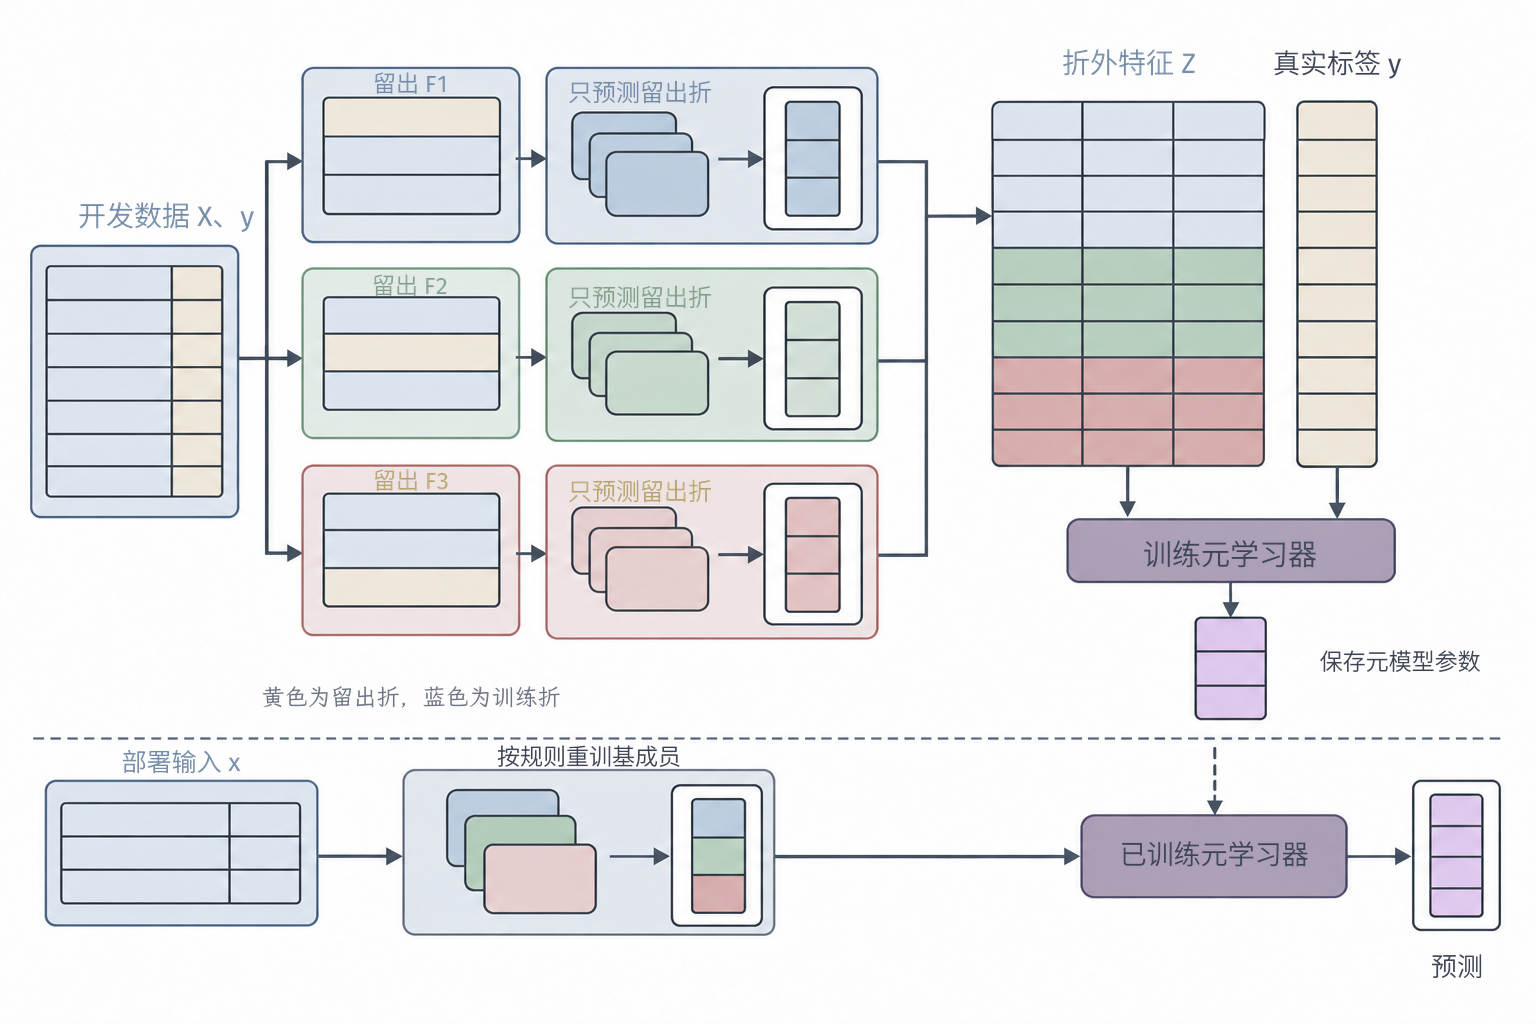
\includegraphics[width=130.048mm]{figures/04-classic-models/00-shared/generated/ensemble-stacking-oof/figure.png}
  \caption{三折Stacking的折外特征构造。每一折轮流作为留出折，临时成员只在其余两折训练，并为留出折产生预测；拼接三次预测得到完整折外矩阵$\bm{Z}$，元学习器以$\bm{Z}$为输入并使用对应标签拟合。部署阶段的基成员还需按预先规定的方式重训或保留。}
  \label{fig:ensemble-stacking-oof}
\end{figure*}

分类成员若输出$C$维概率向量，一个成员通常贡献$C$列元特征；二分类时也可以只保留一个类别概率。类别硬判断省去了得分中的排序或置信信息，不同成员的得分还可能采用不同尺度。元训练与部署使用一致的输出形式，正则化再控制尺度及相关预测对组合的影响。

\paragraph{确定部署成员}

折外矩阵用于训练元学习器，但部署时还需要能预测新输入的基成员。一种做法是在完整训练集上重新拟合每类基学习器$\widehat{h}_m$，预测
\[
  \widehat{y}
  =
  g\!\left(
    \widehat{h}_1(\bm{x}),\ldots,\widehat{h}_M(\bm{x})
  \right).
\]
全量重训利用全部开发数据，但训练规模增加可能改变预测分布，元学习器训练时只看过较小训练集产生的输出。也可保留各折成员，先平均它们对新输入的预测，再送入元学习器；这样沿用折内模型，同时增加了存储与推理次数。两方案的输入分布差异仍由完整验证检验。

部署方案确定后，需要评价基成员与元学习器共同形成的预测流程。基学习器的特征处理、类别编码和超参数搜索必须在相应训练折内完成。若先用全部数据选择特征或编码，再只把模型拟合放进交叉验证，信息仍可能从留出折进入元特征。

\subsubsection{多层组合与输入相关权重}

\paragraph{支持多层组合关系}
\label{sec:ensemble-stacking-multilevel}

若一层组合仍不足以描述成员间关系，可以把中间层输出继续送入下一层。令$\bm a_0(\bm x)=(h_1(\bm x),\ldots,h_M(\bm x))^{\top}$，多层结构写为
\[
 \bm a_\ell(\bm x)=g_{\ell,\bm\theta_\ell}(\bm a_{\ell-1}(\bm x)),
 \quad \ell=1,\ldots,L,
 \qquad H(\bm x)=\bm a_L(\bm x),
\]
其中最后一层维数与所需输出一致。也可把原始特征或较早层输出拼接到某层输入，但须明确拼接对象。训练第$\ell$层时，对每个留出折，都要在其余数据上重新拟合完整下层流程，再为该折产生$\bm a_{\ell-1}$。只让底层成员留出当前记录，而让中间组合层使用其标签，仍会泄漏。逐层增加表达能力的代价是重复拟合、更多参数与部署计算，需要用完整外层验证判断是否值得。

\paragraph{支持输入相关组合}
\label{sec:ensemble-stacking-input-dependent}

固定线性权重让所有输入使用同一组成员贡献。如果线性模型在稀疏区域更稳定、近邻模型在稠密区域更准确，可以让权重随输入改变。一种具体结构是用门控函数$b_m(\bm x;\bm\theta)$产生非负归一化权重：
\[
 w_m(\bm x;\bm\theta)
 =\frac{e^{b_m(\bm x;\bm\theta)}}{\sum_{j=1}^M e^{b_j(\bm x;\bm\theta)}},
 \qquad
 H(\bm x)=\sum_{m=1}^M w_m(\bm x;\bm\theta)h_m(\bm x).
\]
基成员固定后，用折外预测$z_{i,m}$估计门控参数：
\[
 \widehat{\bm\theta}\in\argmin_{\bm\theta}
 \sum_i\ell\!\left(y_i,\sum_m w_m(\bm x_i;\bm\theta)z_{i,m}\right)
 +\lambda\Omega(\bm\theta).
\]
门控输入也须按训练折预处理。部署时把折外预测替换为预定部署成员的输出；各类别概率可以用同一组权重逐类组合。这种加权仍计算全部参与成员，第\ref{sec:ensemble-dynamic-selection}节的动态选择则可进一步只调用一个成员或某个子集。

\subsection{Blending}
\label{sec:ensemble-blending}

\subsubsection{模型结构}

折外构造让每条训练记录都获得一份未使用自身标签的成员预测，却要为每种成员重复拟合多个折内模型。成员训练昂贵时，这个成本可能难以承担。\term{Blending}改用一次留出来构造元特征：把开发数据分为基训练集$D_{\mathrm{base}}$和组合训练集$D_{\mathrm{blend}}$，基成员只在前者拟合，再预测后者，元学习器用这些预测与对应标签训练。每种成员只需一次用于元特征的拟合，代价是两层不再都利用全部开发样本。

\subsubsection{参数学习}

训练数据由两层分用：基成员在$D_{\mathrm{base}}$拟合，元学习器只使用$D_{\mathrm{blend}}$的预测与标签。在开发数据总量固定时，组合训练集$D_{\mathrm{blend}}$占比较小，元学习器用于估计组合关系的记录较少，估计可能不稳定；$D_{\mathrm{blend}}$占比增大，留给基训练集$D_{\mathrm{base}}$的记录随之减少，基成员训练信息也会减少。多次随机划分并平均可以减小单次划分的偶然性，但它重新引入多次训练，已经不再具有单次Blending的全部成本优势。

部署时若把$D_{\mathrm{blend}}$加入基成员重新训练，基预测分布可能相对元学习器训练时发生变化；若不加入，则没有充分利用已有标签。重训方式因此属于模型配置，需要先确定，再用未参与选择的数据评价实际组合。

\Needspace{10\baselineskip}
\subsection{受约束线性Stacking}
\label{sec:ensemble-constrained-linear-stacking}

\subsubsection{模型结构}

成员预测往往高度相关。例如两棵森林只在少量输入上稍有差别，元学习器就可能用很大的正权重与负权重相互抵消，拟合这些细小差异；成员输出稍有变化，组合也会随之放大变化。若希望用较少参数组合，并限制这种抵消，可以把元学习器限制为$b+\bm w^{\top}\bm z$，其中$b$是截距，$\bm w$是成员权重，$\bm z$汇集成员预测。在截距为零且权重非负时，再把权重和限制为一，组合预测就落在成员预测的范围内。

\subsubsection{参数学习}

在回归折外矩阵$\bm{Z}\in\mathbb{R}^{n\times M}$上，可以通过带惩罚的经验目标估计截距与权重：
\begin{equation}
  (\widehat{b},\widehat{\bm{w}})
  \in
  \argmin_{b,\bm{w}}
  \frac{1}{n}
  \sum_{i=1}^{n}
  \ell\!\left(
    y_i,
    b+\bm{w}^{\top}\bm{z}_i
  \right)
  +\lambda\lVert\bm{w}\rVert_2^2.
  \label{eq:ensemble-linear-stacking}
\end{equation}
权重约束控制组合允许的尺度和方向。在$b=0$时，仅要求$w_m\geq0$得到非负线性组合，仍可能放大预测；仅要求$\sum_mw_m=1$得到仿射组合，仍可因负权重而外推。只有同时满足$b=0$、$w_m\geq0$和$\sum_mw_m=1$，才是成员预测的凸组合，输出必定位于成员预测的凸包内。非负约束排除了成员之间的正负抵消，归一化进一步限制整体尺度；有效校正若需要负权重或截距，约束会缩小候选类并增加逼近误差。

权重大小同时受输出尺度、成员相关性和损失函数影响。两个成员预测近乎相同，线性模型可以在它们之间任意分配相近作用；一个成员输出的数值范围更大，也会改变未标准化正则项下的权重。估计权重反映给定尺度、相关性与损失下的联合拟合，而非成员独立贡献。对同一类别集合上的概率向量，使用同一组满足上述凸组合条件的权重逐类组合，结果保持概率单纯形约束，样本外校准再检查概率与实际频率的对应。

\Needspace{10\baselineskip}
\subsection{Super Learner}
\label{sec:ensemble-super-learner}

\subsubsection{模型结构}

不同学习器各有合适的数据条件，事先往往难以指定最佳成员及权重。\term{Super Learner}把候选模型库、折外预测和损失最小化组织成完整程序：用同一套折外数据比较候选，再选择单个成员或学习受约束组合。回归中常用的组合结构为$H(\bm x)=\sum_m w_m h_m(\bm x)$，其中$w_m\geq0$且$\sum_mw_m=1$\scite{vanderlaan2007superlearner}。

\subsubsection{参数学习}

先按式\eqref{eq:ensemble-oof-feature}生成候选库的折外矩阵$\bm Z$。离散版本选择折外平均损失最小的一列；连续组合版本则求解
\[
 \widehat{\bm w}\in\argmin_{\bm w\in\Delta_M}
  \frac1n\sum_{i=1}^n\ell\!\left(y_i,\sum_{m=1}^M w_m z_{i,m}\right),
 \qquad
 \Delta_M=\{\bm w:w_m\geq0,\ \sum_mw_m=1\}.
\]
例如平方损失给出带单纯形约束的最小二乘问题。随后在全部开发数据上重训各基成员，保留已学权重用于组合。候选库也可以预先包含不同模型族和超参数设置，但每列的折外预测必须遵守相应训练范围。

这里的折外损失参与了权重选择，不能再充当整个Super Learner未经选择的最终测试结果。若要比较不同候选库、组合约束或完整Stacking程序，应在外层验证中重新完成内层训练与权重选择。Super Learner与受约束Stacking因此可以共享同一预测结构；前者强调候选库及交叉验证选择程序，后者强调组合层的形式。

\subsection{模型对比与总结}
\label{sec:ensemble-stacking-comparison}

这些方法改变的是组合训练的不同环节。Stacking与Blending分别采用折外预测与一次留出预测；受约束线性组合限制元学习器，多层结构增加组合深度，门控结构使权重依赖输入。Super Learner进一步把候选库和交叉验证损失规定为完整选择程序。表\ref{tab:ensemble-stacking-comparison}据此比较数据安排、组合方式及成本。

\begin{table*}[htbp]
  \centering
  \small
  \begin{tabularx}{\linewidth}{@{}>{\raggedright\arraybackslash}p{25mm}*{5}{>{\raggedright\arraybackslash}X}@{}}
    \toprule
    方法 & 元特征来源 & 数据利用 & 组合规则 & 主要成本 & 主要风险 \\
    \midrule
    Stacking & $K$折折外预测 & 每个样本都产生元特征 & 可线性或非线性 & 每类成员需多次折内拟合 & 折外流程不完整造成泄漏 \\
    Blending & 固定留出集预测 & 元学习器只用留出集 & 可线性或非线性 & 基成员用于元特征时只拟合一次 & 划分敏感与重训分布变化 \\
    受约束线性Stacking & 通常为折外预测 & 与所用划分一致 & 非负、和为一或正则化线性组合 & 组合层较轻量 & 约束可能排除有效校正 \\
    Super Learner & 交叉验证预测与风险 & 由交叉验证方案决定 & 在预定库和组合类中选择 & 候选库越大，训练与选择成本越高 & 候选库遗漏合适模型，或选择过程泄漏 \\
    \bottomrule
  \end{tabularx}
  \caption{Stacking及其代表性变体。表中“数据利用”描述元学习器训练阶段；部署前是否用完整开发数据重训基成员，还需作为流程的一部分单独规定。}
  \label{tab:ensemble-stacking-comparison}
\end{table*}

部署前的全量重训还会改变成员产生预测时所用的训练规模。选择保留折内成员还是重训成员，需要与组合层一起评价，不能只比较各基成员的单独测试结果。比较上述方法时，应固定输出语义、预处理范围和训练预算，再判断新增组合是否改善完整流程的预测。

\section{成员选择与集成简化}
\label{sec:ensemble-selection-compression}

Bagging、Boosting和Stacking先回答怎样形成组合。部署时，多成员推理可能超出内存或延迟预算，一些成员也可能只在局部输入上有用。简化集成有三种不同目标：为所有输入固定一个较小成员子集，针对当前输入临时选择成员，或训练一个新的紧凑模型替代原集成。前两种方法保留部分原成员，第三种方法改变了部署模型。

图\ref{fig:ensemble-selection-compression}沿部署对象区分这三种目标。静态选择把成员池缩成一个固定子集，动态选择保留成员池并让路由依赖当前输入，紧凑化则把完整集成的行为转移到新模型。资源评价据此包括被部署模型以及选择或路由计算。

\begin{figure*}[htbp]
  \centering
  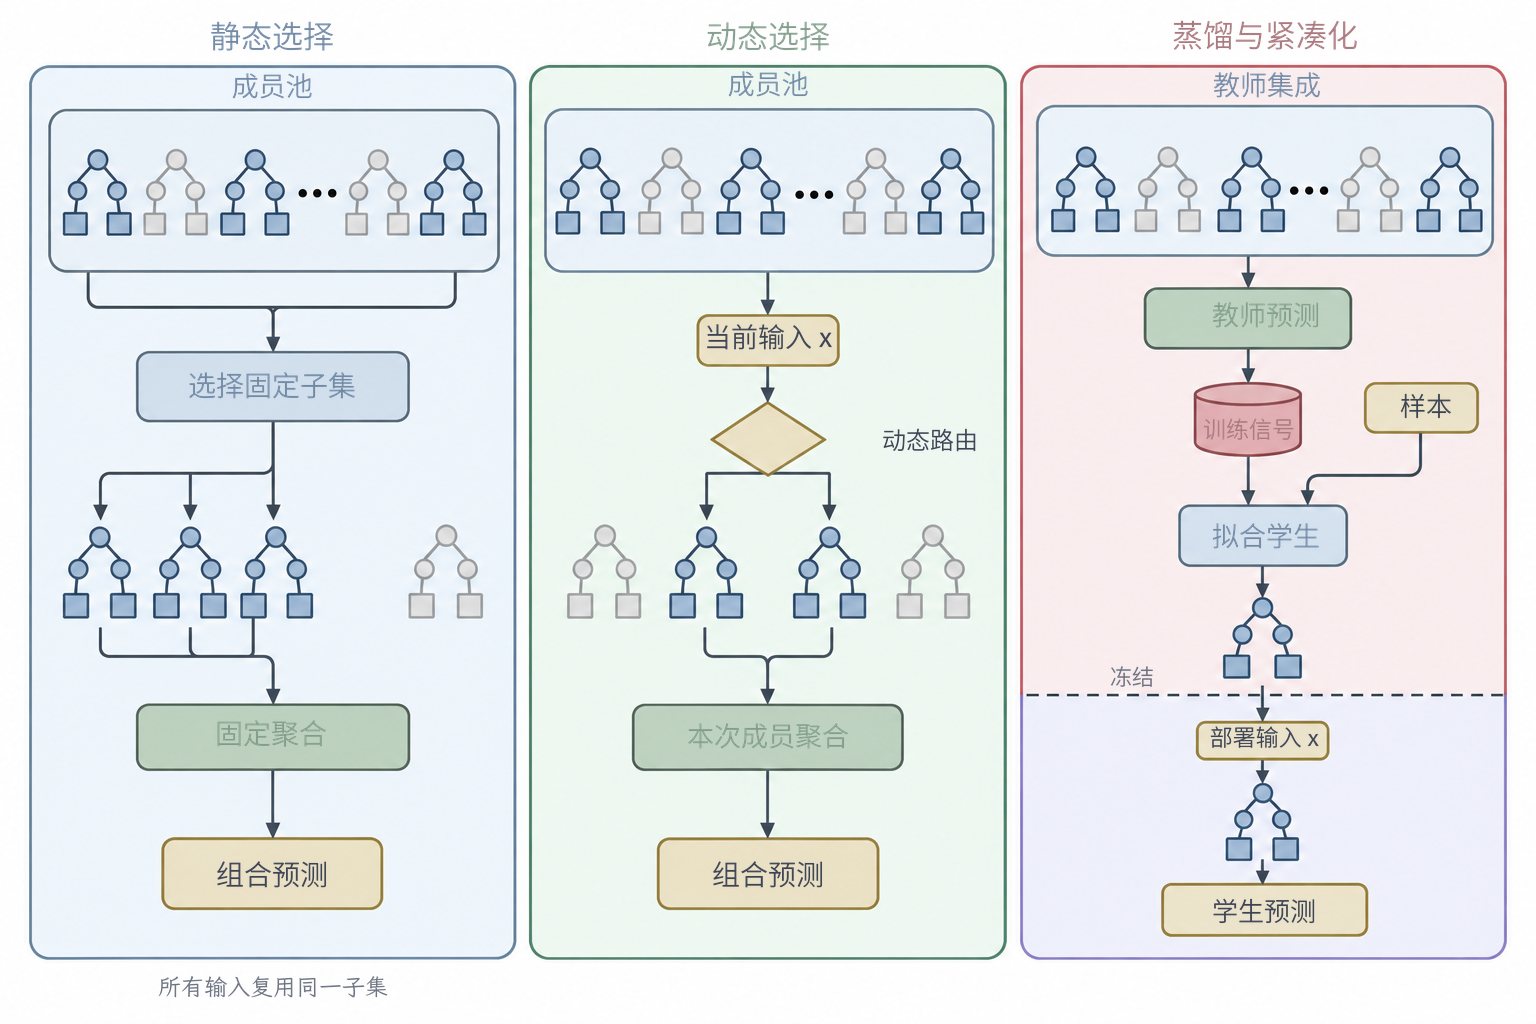
\includegraphics[width=130.048mm]{figures/04-classic-models/00-shared/generated/ensemble-selection-compression/figure.png}
  \caption{静态成员选择、动态成员选择与紧凑化改变的部署对象。静态选择为所有输入保留同一成员子集；动态选择根据输入改变运行成员或组合权重；紧凑化训练并部署新的学生模型。三种路径改变的计算对象不同，成本需沿各自完整路径测量。}
  \label{fig:ensemble-selection-compression}
\end{figure*}

\subsection{静态成员选择}
\label{sec:ensemble-static-selection}

\subsubsection{模型结构}

部署时若只能保留部分成员，我们需要选择在预算内预测效果合适的组合。单模型评分还不足以作出选择：几份预测近乎相同的强成员可能互相重复，加入一个单独误差稍大、但能纠正它们共同错误的成员，反而可能得到更好的组合。\term{静态成员选择}（static ensemble selection）从已经训练好的候选池$\{h_1,\ldots,h_M\}$中，选择一个对所有未来输入都相同的非空子集$S\subseteq\{1,\ldots,M\}$，评价对象是整个子集的组合预测。

\subsubsection{参数学习}

若$\mathcal{L}_{\mathrm{val}}(S)$表示该组合的平均验证损失，可以用损失与部署成本共同选择子集：
\begin{equation}
  \widehat{S}
  \in
  \argmin_{\varnothing\neq S\subseteq\{1,\ldots,M\}}
  \mathcal{L}_{\mathrm{val}}(S)
  +\lambda_1|S|
  +\lambda_2 C(S),
  \label{eq:ensemble-static-selection}
\end{equation}
其中$\lambda_1,\lambda_2\geq0$，$|S|$控制成员数，$C(S)$可以表示存储、单样本延迟或其他部署成本。成员池包含指数多个子集，实际可用排序、逐个加入或删除等方法近似搜索，并记录所得子集的验证损失与资源成本。

单成员排序忽略预测的重叠，可能同时保留许多相似模型。前向选择则评价候选加入当前组合后的损失变化，使选择依赖已有成员。允许重复选择某个成员时，重复次数还形成离散权重。基于模型库的贪心集成选择就是这种做法的代表：从一个初始组合出发，每轮加入使验证指标改善最大的候选，必要时使用多起点或装袋法减少搜索的不稳定性\scite{caruana2004ensemble}。

式\eqref{eq:ensemble-static-selection}的搜索对象为固定池中的成员子集，成员预测已经形成。若同时改变基学习算法、特征处理和超参数，搜索范围已经扩展为完整模型开发流程。候选池越大，验证集上偶然出现有利组合的机会也越多；最终测试需在该子集及其组合规则固定后进行。

\subsection{动态成员选择}
\label{sec:ensemble-dynamic-selection}

\subsubsection{模型结构}

静态方案让所有输入使用相同子集，却可能遗漏成员能力随输入改变的情况。假设一个文本分类器在体育报道附近的预测可靠，另一个在科技报道附近更可靠，用全体文档上的平均正确率排序，就可能忽略这种局部差别。我们可以在独立数据中寻找与当前输入邻近的记录，比较成员在这些记录上的表现，再决定调用谁。\term{动态分类器选择}（dynamic classifier selection, DCS）为每个输入选择一个成员；\term{动态集成选择}（dynamic ensemble selection, DES）选择一个成员子集或给出输入相关权重。

\subsubsection{参数学习}

一种基本构造是准备独立的能力估计数据。对查询输入$\bm{x}$，在该数据中寻找非空邻域$\mathcal{N}(\bm{x})$，再以成员$m$在邻域内的正确率估计
\begin{equation}
  \widehat{c}_m(\bm{x})
  =
  \frac{1}{|\mathcal{N}(\bm{x})|}
  \sum_{i\in\mathcal{N}(\bm{x})}
  \mathbb{I}\!\left\{h_m(\bm{x}_i)=y_i\right\}.
  \label{eq:ensemble-local-competence}
\end{equation}
DCS可以选择$\widehat{c}_m(\bm{x})$最大的成员，DES则保留超过阈值的成员或按能力加权。局部正确率只是能力估计的一种方式，还可以使用输出轮廓、分类间隔或由元模型学习的能力特征\scite{woods1997localaccuracy}。

局部选择依赖邻域和能力估计两部分。邻域依赖输入表示与距离，高维或分布稀疏时，附近样本未必提供稳定的局部证据；能力估计器也可能在有限数据上过拟合。成员训练数据、能力估计数据与最终测试数据需要分开，所有标准化和邻域参数都在相应开发流程内确定。

动态选择的延迟由路由和实际运行成员共同决定。若系统必须先运行全部成员才能构造输出轮廓，再选择其中几个聚合，选择之前已经支付全部成员计算；基于输入邻域的方法还增加了检索成本。在昂贵成员运行前完成路由，才可能直接省去被跳过成员的计算；局部检索、路由和输出质量需要一并测量。

\subsection{从集成模型到紧凑模型}
\label{sec:ensemble-compression}

\subsubsection{模型结构}

若原成员的最小可用子集仍超预算，可以另外训练一个新的\term{紧凑模型}（compact model），使其逼近完整集成的输入输出映射。早期模型压缩工作已经用大型集成的输出训练较小模型；知识蒸馏随后把这种教师到学生的传递扩展为常用训练形式\scite{bucilua2006compression,hinton2015distilling}。

\subsubsection{参数学习}

设完整集成为教师$H$，紧凑模型为学生$s_{\bm{\theta}}$。对回归，可以组合真实响应损失与教师拟合损失：
\begin{equation}
  \min_{\bm{\theta}}
  \sum_{i=1}^{n}
  \left[
    \alpha\ell\!\left(y_i,s_{\bm{\theta}}(\bm{x}_i)\right)
    +(1-\alpha)
    \ell\!\left(H(\bm{x}_i),s_{\bm{\theta}}(\bm{x}_i)\right)
  \right],
  \label{eq:ensemble-compression-objective}
\end{equation}
其中$\alpha\in[0,1]$控制真实标签与教师输出的作用。分类时可以拟合教师的完整类别分布；温度缩放会使非最大类别之间的相对关系更容易进入训练信号，但温度、损失权重与部署概率仍须分别选择和校准。

学生训练输入可以来自原训练集、额外未标注样本或经过说明的合成样本。教师在所选输入上提供训练目标；覆盖不足的区域缺少这种监督，学生在这些区域仍可能偏离教师。学生容量过小会产生逼近误差，容量很大则可能无法达到预期资源节省。


\Needspace{18\baselineskip}
\section{本章小结}
\label{sec:ensemble-summary}

集成利用成员生成与组合规则改变预测误差。互补作用来自成员能够在部分输入上修正彼此的判断，共同遗漏的结构仍需改变表示或训练方式。Bagging通过样本、特征或分裂随机性构造可并行成员，再用平均或投票削弱一部分训练波动；Boosting让每轮成员依赖当前组合，沿选定损失逐步加入修正；Stacking使用折外预测训练元学习器，使组合规则本身也由数据决定。三类机制可以嵌套，但各自的数据依赖、计算路径和失效原因不同。

成员池形成后，还可以改变部署规模。静态成员选择为所有输入固定同一子集，动态成员选择针对当前输入估计局部能力，紧凑化则训练一个新模型逼近完整集成。选择保留原成员的部分计算，紧凑化则部署一个重新训练的预测器，因此其成本与误差来源需要分别评价。

三类方法的改进需要放在完整预测流程中判断。Bagging的成员可以并行训练，Boosting的轮次相互依赖，Stacking则同时承担基成员与组合层的计算；相同成员数并不意味着相同容量或成本。比较时应使用同一输出目标、数据划分和调参预算，同时检查任务损失、概率质量、模型大小以及包含预处理、全部成员和路由的端到端延迟。

图\ref{fig:ensemble-data-isolation}概括了不同留出预测的职责。袋外预测用于Bagging内部诊断，折外预测用于训练Stacking组合层，能力估计预测用于动态选择，验证预测用于确定配置；这些结果都可能影响模型开发。最终测试只评价成员、组合、校准和部署规则全部冻结后的流程。预处理、成员筛选和超参数搜索也必须留在相应训练范围内，不能只隔离最后一次模型拟合。后续神经网络模型部分将在这些原则上讨论初始化、样本顺序与训练过程产生的神经网络集成。

\begin{figure*}[htbp]
  \centering
  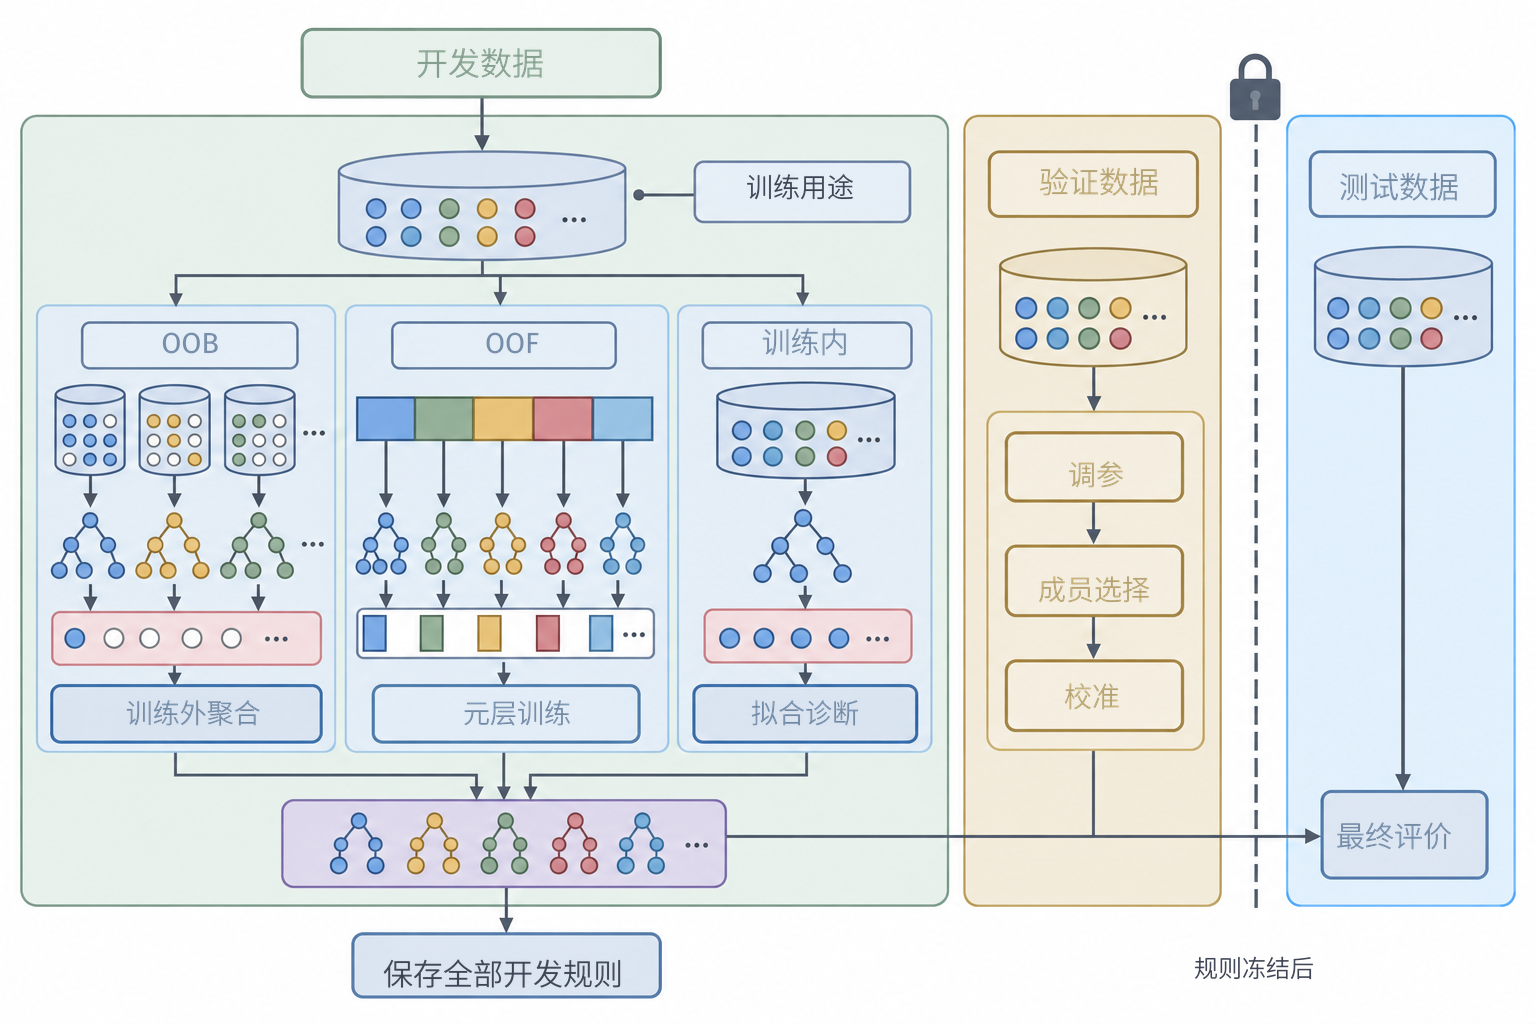
\includegraphics[width=130.048mm]{figures/04-classic-models/00-shared/generated/ensemble-data-isolation/figure.png}
  \caption{集成学习中的数据隔离与预测职责。开发阶段的预测及验证数据各有规定用途；测试阶段前的竖直分隔线表示训练、调参、筛选、校准和部署规则已经冻结。测试预测评价已经冻结的流程；图中不向开发步骤返回选择信号。}
  \label{fig:ensemble-data-isolation}
\end{figure*}

\paragraph{扩展阅读}
Hastie等的教材从加法建模解释提升方法；Breiman的Bagging与随机森林论文说明重采样及特征随机化的作用。可选同一预测任务，比较成员误差中可被组合削弱的部分，并记录获得这一收益所需的训练与部署成本\scite{hastie2009,breiman1996bagging,breiman2001randomforests}。

